% 本文件定位：性爱实践卷（前戏、爱抚、技巧、体位与姿势、安全事项）

\documentclass[12pt,UTF8]{ctexbook}

% 设置纸张信息
\usepackage[a4paper]{geometry}
\geometry{
    inner=2cm,
    outer=2cm,
    top=2.5cm,
    bottom=2.5cm
}

% 设置字体
\usepackage{xeCJK}
\setCJKmainfont{SimSun}[BoldFont=SimHei, ItalicFont=KaiTi]
\setCJKsansfont{SimHei}
\setCJKmonofont{SimSun}

% ===== 符号字体回退（r75）：带圈数字 / 罗马数字 / 希腊字母 / 数学符号 / 制表符 ----
%   背景：西文主字体 Latin Modern 与中文字体 SimSun 均不覆盖下列字符，
%   不回退则 xelatex 报 Missing character，PDF 对应位置留白（等于丢知识点）。
%   自检：编译后统计 <file>.log 中 Missing character 条数，应为 0。
\usepackage{newunicodechar}
\newfontfamily\symbolfallback{SimSun}           % 带圈数字/罗马数字/希腊字母/数学符号/制表符/几何图形
\newfontfamily\symbolfallbackx{Segoe UI Symbol} % 警告三角等符号
\newunicodechar{①}{{\symbolfallback\char"2460}}
\newunicodechar{②}{{\symbolfallback\char"2461}}
\newunicodechar{③}{{\symbolfallback\char"2462}}
\newunicodechar{④}{{\symbolfallback\char"2463}}
\newunicodechar{⑤}{{\symbolfallback\char"2464}}
\newunicodechar{⑥}{{\symbolfallback\char"2465}}
\newunicodechar{⑦}{{\symbolfallback\char"2466}}
\newunicodechar{⑧}{{\symbolfallback\char"2467}}
\newunicodechar{⑨}{{\symbolfallback\char"2468}}
\newunicodechar{⑩}{{\symbolfallback\char"2469}}
\newunicodechar{Ⅰ}{{\symbolfallback\char"2160}}
\newunicodechar{Ⅱ}{{\symbolfallback\char"2161}}
\newunicodechar{Ⅲ}{{\symbolfallback\char"2162}}
\newunicodechar{Ⅳ}{{\symbolfallback\char"2163}}
\newunicodechar{Ⅴ}{{\symbolfallback\char"2164}}
\newunicodechar{Ⅵ}{{\symbolfallback\char"2165}}
\newunicodechar{Ⅶ}{{\symbolfallback\char"2166}}
\newunicodechar{Ⅷ}{{\symbolfallback\char"2167}}
\newunicodechar{Ⅸ}{{\symbolfallback\char"2168}}
\newunicodechar{Ⅹ}{{\symbolfallback\char"2169}}
\newunicodechar{Ⅺ}{{\symbolfallback\char"216A}}
\newunicodechar{Ⅻ}{{\symbolfallback\char"216B}}
\newunicodechar{α}{{\symbolfallback\char"03B1}}
\newunicodechar{β}{{\symbolfallback\char"03B2}}
\newunicodechar{γ}{{\symbolfallback\char"03B3}}
\newunicodechar{δ}{{\symbolfallback\char"03B4}}
\newunicodechar{ε}{{\symbolfallback\char"03B5}}
\newunicodechar{ζ}{{\symbolfallback\char"03B6}}
\newunicodechar{η}{{\symbolfallback\char"03B7}}
\newunicodechar{θ}{{\symbolfallback\char"03B8}}
\newunicodechar{ι}{{\symbolfallback\char"03B9}}
\newunicodechar{κ}{{\symbolfallback\char"03BA}}
\newunicodechar{λ}{{\symbolfallback\char"03BB}}
\newunicodechar{μ}{{\symbolfallback\char"03BC}}
\newunicodechar{ν}{{\symbolfallback\char"03BD}}
\newunicodechar{ξ}{{\symbolfallback\char"03BE}}
\newunicodechar{ο}{{\symbolfallback\char"03BF}}
\newunicodechar{π}{{\symbolfallback\char"03C0}}
\newunicodechar{ρ}{{\symbolfallback\char"03C1}}
\newunicodechar{ς}{{\symbolfallback\char"03C2}}
\newunicodechar{σ}{{\symbolfallback\char"03C3}}
\newunicodechar{τ}{{\symbolfallback\char"03C4}}
\newunicodechar{υ}{{\symbolfallback\char"03C5}}
\newunicodechar{φ}{{\symbolfallback\char"03C6}}
\newunicodechar{χ}{{\symbolfallback\char"03C7}}
\newunicodechar{ψ}{{\symbolfallback\char"03C8}}
\newunicodechar{ω}{{\symbolfallback\char"03C9}}
\newunicodechar{≠}{{\symbolfallback\char"2260}}
\newunicodechar{≈}{{\symbolfallback\char"2248}}
\newunicodechar{≤}{{\symbolfallback\char"2264}}
\newunicodechar{≥}{{\symbolfallback\char"2265}}
\newunicodechar{─}{{\symbolfallback\char"2500}}
\newunicodechar{■}{{\symbolfallback\char"25A0}}
\newunicodechar{⚠}{{\symbolfallbackx\char"26A0}}

% 目录格式
\usepackage{titletoc}
\titlecontents{chapter}[0pt]{\vspace{3mm}\bf}{\contentspush{\thecontentslabel\hspace{1em}}}{}{\titlerule*[8pt]{.}\contentspage}

% 图片相关设置
\usepackage{graphicx}
\usepackage{float}
\graphicspath{{Images/}}

% 颜色支持
\usepackage{color}

% 绘制流程图
\usepackage{tikz}
\usetikzlibrary{shapes,arrows,positioning,calc}

% 表格相关设置
\usepackage{tabularx}
\usepackage{booktabs}

% 彩色盒子环境
\usepackage{tcolorbox}

% 术语表和索引
\usepackage{glossaries}
\usepackage{makeidx}
\makeindex
\makeglossaries

% BibTeX参考文献支持
\usepackage{natbib}
\bibliographystyle{plainnat}

% 页眉页脚
\usepackage{fancyhdr}
\pagestyle{fancy}
\lhead{}
\chead{}
\rhead{\bfseries \leftmark}
\lfoot{}
\cfoot{\thepage}
\rfoot{}
\renewcommand{\headrulewidth}{0.4pt}
\renewcommand{\footrulewidth}{0pt}

% 段落间距
\setlength{\parskip}{0.5em}
\setlength{\parindent}{2em}

% 目录格式设置
\usepackage{titletoc}
\usepackage{enumitem}% 支持 \begin{itemize}[leftmargin=2cm] 等带可选参数的列表（与 male.tex 一致）
\titlecontents{chapter}[0pt]{\vspace{3mm}\bfseries}{\thecontentslabel\hspace{1em}}{}{\titlerule*[8pt]{.}\contentspage}[\vspace{2mm}]
\titlecontents{section}[3em]{\contentslabel[\thecontentslabel]{2em}\hspace{1em}}{}{}{\titlerule*[6pt]{.}\contentspage}
\titlecontents{subsection}[5em]{\contentslabel[\thecontentslabel]{3em}\hspace{1em}}{}{}{\titlerule*[4pt]{.}\contentspage}

% 标题格式
\ctexset{
    part/name={第,篇},
    part/number={\chinese{part}},
    chapter/name={第,章},
    chapter/number={\chinese{chapter}}
}

% 章节摘要环境
\newenvironment{chapterabstract}[1][摘要]{
    \vspace{0.5em}
    \begin{center}\bfseries{#1}\end{center}
    \vspace{0.5em}
    \begin{quote}
    }{
    \end{quote}
    \vspace{0.5em}
}

% 重点标记
\newcommand{\keyterm}[1]{{\bfseries #1}}
\newcommand{\important}[1]{{\color{red} \bfseries #1}}

% 关键论断/关键词强调（《两性研究导论》章使用；视觉同 \keyterm，语义上作区分）
\newcommand{\keyword}[1]{\textbf{#1}}

\title{\heiti\zihao{0} 性爱实践指南}
\author{}
\date{}

\begin{document}

\maketitle

\frontmatter

\chapter{前言}

本书是《性学大全指南》的\keyword{性爱实践卷}，独立于共通卷（book.tex）、女性卷（female.tex）与男性卷（male.tex）单独成册，
内容聚焦于\keyword{性行为本身}——前戏与爱抚、亲密技法、性交体位与姿势、辅助器具与安全事项。

分五篇：第一篇　亲密与准备；第二篇　前戏与爱抚；第三篇　性技巧与实践；第四篇　性交体位与姿势；第五篇　安全与应对。

\begin{tcolorbox}[colback=pink!5!white,colframe=red!50!black,title=使用说明]
本卷讲的是“怎么做”，不重复讲“为什么会这样”——生理机制、疾病诊治、心理与社会议题在其余三卷。体位与技巧的价值在于\keyword{舒适与默契}，不在于难度或数量；任何造成疼痛的做法都应立即调整或停止。
\end{tcolorbox}

\tableofcontents

\listoffigures
\listoftables

\mainmatter

\part{亲密关系与基础准备}

\chapter{情感亲密与性沟通}

很多人翻开一本两性的书，第一反应是直接翻到“技巧”那一章。但现实是，绝大多数的性生活不和谐，根源根本不在身体，而在关系。

如果你在日常相处中充满怨气，床上的前戏就会变成机械的敷衍；如果你连“我想要什么”都不敢开口，再高超的技巧也只是闭着眼睛瞎撞。

所以，我们把这本书的第一章留给了“情感”与“沟通”。这不是在说教，而是想帮你打好最坚实的地基。本章我们先不碰身体，先来解决三个问题：怎么让关系重新升温？怎么把话聊到心坎里？怎么理直气壮地表达需求和拒绝？记住，最好的春药，永远是安全感和深深的信任。

\section{情感亲密的建立与维护}

情感亲密是性亲密的最强催化剂。很多时候，比起单纯的生理技巧，伴侣间深厚的情感联结才是获得极致愉悦的基础。在本节中，我们将探讨情感亲密是如何构成的，如何在日常生活中储蓄情感，以及在冲突后如何进行关系修复。

\subsection{情感亲密的基石与体现}

情感亲密（Emotional Intimacy）指伴侣之间在情感层面的靠近与敞开。它与性亲密不同，却常是性亲密的重要基础。研究者通常把情感亲密拆解为几个可辨识的核心要素，这些要素共同构成了“我们”这一感受的基础：

\begin{itemize}
\item \textbf{自我表露（脆弱与坦诚）}：愿意分享内心的想法、恐惧与脆弱，敢于展露真实的自我，而不必担心被评判。表露是亲密的前提，不了解就无从亲近。
\item \textbf{伴侣回应性（被看见与接纳）}：一方的表露得到另一方的关注、理解与重视。这种专注的在场使表露变得安全，从而鼓励更多表露。
\item \textbf{相互接纳}：在了解对方的优点与缺点之后，仍然选择接纳。这使得亲密建立在对真实的人的认识之上，而非对想象中的完人。
\item \textbf{共同意义}：双方共享的价值观、记忆与关于关系的叙述，构成了“我们”的内容基础。
\item \textbf{非性接触的亲密}：日常的拥抱、牵手、轻抚，这些不以性交为目的的肢体接触，是维系情感亲密不可或缺的载体。
\end{itemize}

一个关键的认识是：亲密不是一次完成的成就，而是需要持续投入的过程。研究显示，伴侣之间的自我表露水平若长期下降（如只剩下事务性交流），情感亲密度也会随之降低。因此，维持亲密的关键不在于“我们曾经多亲密”，而在于“我们最近还在彼此敞开吗”。

\begin{tcolorbox}[colback=pink!5!white,colframe=red!50!black,title=贴心小叮咛]
亲密不是“我懂你”这种默契，而是“我愿意让你看见我”这种敞开。它需要有人先开口，也需要另一个人好好接住。
\end{tcolorbox}

\subsection{日常互动与情感储蓄}

情感亲密最主要的部分，发生在日常的微小互动中，而非重大时刻。心理学家约翰·戈特曼（John Gottman）用“情感银行账户”这一比喻来描述：每一次关注、回应、感谢与善意，都是向关系账户里存入的一笔；而忽视、冷淡、指责与轻蔑则是支出。

这一比喻改变了关系维护的着力点。许多人以为关系要靠“大动作”来维护——旅行、礼物、纪念日的惊喜。这些当然有用，但研究显示，日常微小互动的累积对关系质量的预测力更强。因为它们发生频率极高，日积月累的效应远超偶发的大事件。你可以从以下具体行为入手进行“存款”：

\begin{itemize}
\item \textbf{主动回应}：对方分享时给予关注，而非敷衍或转移话题。
\item \textbf{具体感谢}：说出具体感谢的事（比如“谢谢你今天顺手把衣服收了”），比笼统的“谢谢你”更有效。
\item \textbf{创造专属连接}：建立属于两人的小仪式，比如每周的约会夜、睡前十分钟“只聊天不解决问题”的时间。
\item \textbf{身体接触}：拥抱、牵手、搭肩等日常接触，维持身体的亲近感。
\item \textbf{注意小事}：记住对方提过的事，并适时提起。
\end{itemize}

与之相对，最需要避免的是“轻蔑”这一互动形式。关系研究者发现，在各类负面互动中，轻蔑（表现为讽刺、嘲笑、翻白眼、贬低）对关系的预测力最强，甚至强于争吵本身。轻蔑的核心信号是“我不尊重你”，它直接否定对方作为人的价值，因而伤害最深。

实践上，一个有效的框架是“转向”与“转开”。伴侣之间会不断发出微小的“连接请求”——说一句无关紧要的话、指一下窗外的景、叹一声气。若对方选择“转向”（回应、接话、表示关注），关系账户存入一笔；若选择“转开”（忽视、打断、继续自己的事），则支出一笔。研究显示，长期保持高“转向率”的伴侣，其关系稳定性显著更高。

\begin{tcolorbox}[colback=pink!5!white,colframe=red!50!black,title=贴心小叮咛]
关系不是靠几次旅行撑起来的，而是靠每天那些看起来无关紧要的小回应。对方开口的时候，你有没有接住——这件小事重复几千次，就成了你们关系的底色。
\end{tcolorbox}

\subsection{冲突化解与关系修复}

冲突本身对关系的伤害，远不如冲突后未能修复来得大。未解决的冲突会变成性的阻碍，因为身体在感到不安全时很难完全敞开。关系研究中一个稳定的发现是：预测关系存续的，不是争吵的频率，而是修复的能力。

修复的第一步是中断升级。冲突中的恶性升级通常表现为几种模式：翻旧账、人身攻击（从具体问题转向对方的人格），以及“四骑士”式的反应（批评、防御、轻蔑、冷战）。识别这些模式并主动中断，是修复的前提。可行的做法包括明确喊停（“我们停一下，我有点上头了”）、约定冷静期（如半小时后再谈），以及暂时转移话题。

\begin{itemize}
\item \textbf{及时中断}：识别升级信号，主动喊停或约定冷静期。
\item \textbf{就事论事}：在表达时使用“我感觉……”的句式，而不是“你总是……”的指责。
\item \textbf{先处理关系}：在讨论问题前，先恢复彼此的连接与安全感。
\end{itemize}

第二步是恢复连接。关系中有一个重要概念叫“修复尝试”（repair attempt）——即在冲突中发出的、意在缓和关系的信号，可能是一句幽默、一个表情、一次触碰、或者一句“我不想和你吵”。研究发现，能够识别并接住这些信号的伴侣，其冲突的破坏性显著较低。关键在于：修复尝试往往很微小，容易被忽略，而能否接住它们决定了能否从冲突中走出来。

\begin{itemize}
\item \textbf{承担自己的部分}：不必全盘认错，但可以承认自己应负的部分。
\item \textbf{具体道歉}：说出道歉的具体内容，避免“对不起行了吧”式的敷衍。
\item \textbf{修复尝试}：一个玩笑、一个拥抱、一句“我们别吵了”，都是有效的修复信号。
\end{itemize}

第三步才是处理实际问题。顺序很重要：先恢复关系层面的安全与连接，再回到具体问题。反过来做——在情绪未平复时强行“把问题讲清楚”——通常只会引发新一轮升级。此外，有效道歉的要素包括：明确说出自己做了什么、承认对方因此受到影响、表达懊悔、以及说明将如何改变，而不是含混的“对不起”。

\begin{tcolorbox}[colback=pink!5!white,colframe=red!50!black,title=贴心小叮咛]
吵架不可怕，吵完之后没人先开口才可怕。一句“我们别吵了”，或者只是递杯水，往往就是关系的转折点——而它有九成的概率，需要你来做。
\end{tcolorbox}

\section{伴侣间的性沟通}

\subsection{开启性话题的时机与方式}

谈性议题最容易失败的原因，往往不是内容本身，而是时机与方式。同样的内容，在合适的条件下能顺利展开，在错误的条件下则必然引发冲突或回避。

\textbf{一、避开时机雷区}

时机方面，有几类明确应当避开的情形。第一是在卧室里、性活动进行中或刚结束时提出批评性的内容——此时双方处于最脆弱的暴露状态，任何负面反馈都容易被体验为人身否定。第二是在冲突中或情绪激动时提起性议题——性话题极易成为攻击武器。第三是在疲惫、匆忙或有他人在场时。研究显示，这类时机的失败率极高，且会造成“谈了也没用”的负面预期，使日后再开口更加困难。

\begin{itemize}
\item \textbf{避开卧室}：不在床上、不在性活动前后讨论敏感议题。
\item \textbf{避开冲突}：不在争吵中提起性，避免它成为攻击手段。
\item \textbf{避免高压}：不在疲惫、匆忙或有他人在场时开启话题。
\end{itemize}

\textbf{二、创造安全的对话空间}

方式方面，核心是保持双向与低压。具体的可行做法包括：

\begin{itemize}
\item \textbf{选定专门时段}：在放松、私密、无时间压力的条件下进行。
\item \textbf{从轻松话题入手}：由偏好、兴趣等中性内容开始，而非直接进入不满。
\item \textbf{使用“我”语句}：以“我喜欢……”而非“你怎么老是……”来表达。
\item \textbf{保持双向}：既说自己的需求，也主动询问对方的感受。
\item \textbf{明确邀请}：表达这不是要求而是邀请（“要不要试试看”），并允许对方不参与。
\end{itemize}

这些做法看起来简单，但研究显示它们能显著降低对方的防御反应。

\textbf{三、将沟通制度化}

另一个实用做法是“设定一个固定的谈论时间”。若把性议题纳入定期的关系检视（如每月一次），它就不再是“出问题了才提”的尴尬事项，而成为关系维护的常规组成部分。这一制度化降低了开门的心理成本，也使双方都有心理准备，不会措手不及。

\begin{tcolorbox}[colback=pink!5!white,colframe=red!50!black,title=贴心小叮咛]
谈性失败，多半不是因为话题本身，而是因为说得不是时候。请把这句话记住：不在床上说，不在吵架时说，找个白天，坐下来慢慢说。
\end{tcolorbox}

\subsection{倾听、回应与非语言沟通}

性沟通包含两个同样重要的能力：表达与倾听。多数人只关注前者，而实践中的瓶颈往往在后者。

\textbf{一、如何有效表达}

表达的核心要求是“具体”。笼统的表达几乎无法执行：“我希望你更主动”留下了太多解释空间；而“我希望偶尔你能先亲我一会儿，再开始”则是明确可操作的。此外，表达应包含正向内容：不只是提出希望改变的部分，也要说出自己欣赏的地方。研究显示，具体的肯定比笼统的赞美更有价值——因为它指出了可以重复的方向。

\begin{itemize}
\item \textbf{具体化}：描述具体的行为、部位、节奏，避免笼统的表述。
\item \textbf{正向优先}：先说你喜欢什么，再提出希望调整的部分。
\item \textbf{使用“我”语句}：用“我感到……”表达，减少对方被指控的感受。
\end{itemize}

\textbf{二、如何深度倾听}

倾听能力更为稀缺，也更关键。倾听的第一个要求是不打断、不辩解。当一方鼓起勇气说出需求时，另一方最常见的反应是解释或反驳（“我没有那样吧”“那是因为你……”），这类反应会让说话者感到“说了也没用”，从此关闭沟通。更有效的做法是先完整听完，再回应；即便不同意，也可以先承认对方的感受是真实的。

倾听的第二个要求是确认理解。复述对方的内容（“你的意思是说，你希望我……对吗”）能显著减少误读，也让对方感到被认真对待。研究显示，被准确理解的体验本身即有强烈的安抚作用，往往比问题是否被解决更重要。

\begin{itemize}
\item \textbf{倾听不反驳}：对方表达时先完整听完，不打断、不辩解。
\item \textbf{确认理解}：复述对方的意思以确认，避免误读。
\item \textbf{识别弦外之音}：注意对方未直说的部分，例如抱怨背后隐藏的渴望。
\end{itemize}

\textbf{三、读懂非语言信号}

除了用嘴说和用耳朵听，性沟通中绝不可忽视的是“非语言沟通”。在卧室里，身体往往比语言更诚实，尤其在双方都难以启齿的时候。

\begin{itemize}
\item \textbf{眼神接触}：温柔的目光接触能极大增强亲密感与安全感。反之，全程闭眼或频繁避开视线，可能暗示着羞耻、走神或隐藏的不适。
\item \textbf{肢体语言}：主动的靠近、迎合与拥抱是接纳的信号；而身体僵硬、下意识地退缩或挡住某些部位，则是在表达抗拒或紧张。
\item \textbf{语气语调}：同样一句“我想要”，急促高亢显得急躁，轻柔低缓则充满情欲。降低音量、放慢语速，能有效降低对方的防御机制。
\item \textbf{解读身体反应}：呼吸急促、肌肉紧绷或放松、主动迎合与退缩，这些都是最直接的“身体反馈”。学会敏锐地捕捉这些信号，并及时调整节奏，比任何技巧都管用。
\end{itemize}

需要提醒的是，非语言沟通虽然真实，但也极其容易产生误读。比如，对方屏住呼吸可能是极度投入，也可能是因为疼痛在忍耐。因此，最安全的做法是：在事后温存时，用语言去确认那些你不确定的非语言信号（“刚刚你突然抱紧我，是感觉很好吗？”），这样既能避免误会，又能进一步提升默契。

\begin{tcolorbox}[colback=pink!5!white,colframe=red!50!black,title=贴心小叮咛]
对方说出一件难以启齿的事，需要的不是你的解释，而是你先把话听完。一句“我知道了，谢谢你告诉我”，比任何辩护都更能让人愿意继续说下去。
\end{tcolorbox}

\subsection{打破谈性的常见障碍}

性沟通中的障碍有几类反复出现的模式。识别这些模式，可以在它们发生时及时调整。常见的障碍包括：人身化解读、期待读心、积压后爆发，以及单向输出。

\begin{itemize}
\item \textbf{人身化解读}：把具体反馈听成人身评价，从而触发防御。
\item \textbf{期待读心}：认为“真爱就该懂”，把说出需求视为无奈之举。
\item \textbf{积压后爆发}：长期隐忍，最后以总清算的形式一并倒出。
\item \textbf{单向输出}：只有一方提要求，另一方被动配合，导致关系失衡。
\end{itemize}

\textbf{第一类：情绪化解读（人身化解读）}

性话题极度敏感，任何反馈都容易被解读为人身评价。指出一个具体的不适，可能被听成“你不行”；表达一个偏好，可能被听成“你一直做错了”。这种解读会自动触发防御，使对话迅速偏离原题。破解的方法是在开口前先做铺垫（“我想说的只是我喜欢什么，不是说你不好”），以及在听到时主动确认（“你是在说方式的问题，还是在说别的”）。

\textbf{第二类：期待读心}

它源于浪漫文化中“灵魂契合”的叙述，使人把“需要我说出来”看作关系不够好的证据。但性偏好高度个体化，没有任何人能凭直觉准确猜中。把表达需求视为正常协商而非关系缺陷，是破解这一障碍的关键。

\textbf{第三类：积压后爆发}

一方长期隐忍不满，直到某个导火索引爆，把陈年旧账一并倾泻。此时对方猝不及防，双方都感到被攻击。更有效的是及时、小剂量地反馈：在体验发生后的次日，以平和的方式说出一两点。这样既保持了情境的清晰，也避免了情绪过载。

\textbf{第四类：单向输出}

若关系中只有一方不断提出要求，另一方持续被动配合，关系会逐渐失衡——配合方可能感到被当作工具，提出方则可能因得不到主动回应而更焦虑。健康的方向是双向的：不仅说出自己要什么，也主动关心对方要什么。

\begin{tcolorbox}[colback=pink!5!white,colframe=red!50!black,title=贴心小叮咛]
大多数“谈了也没用”的经历，问题不在谈，而在话积得太久、挑的时机太差。早说、少说、分开说，比憋到最后一次说完要有效得多。
\end{tcolorbox}

\section{性需求的表达与边界}

\subsection{识别自身需求与偏好}

表达需求的前提是识别需求，而这恰恰是许多人卡住的地方。长期压抑自身需求的人，往往真的说不清自己想要什么——这不是拒绝沟通，而是需求识别本身需要练习。

\textbf{一、如何识别自身需求}

需求识别可以从几个方向入手。第一是回顾经验：回想过去哪些时刻体验较好，具体是什么因素让它好——是节奏、特定的接触方式、某种氛围、还是某个时段？把模糊的“感觉不错”拆解为具体要素。第二是留意反应：在自慰或性活动中，注意身体对什么有正向反应，哪怕只是轻微的变化。第三是接纳“不确定”：承认自己暂时不知道想要什么，也是一种状态。

\begin{itemize}
\item \textbf{回顾经验}：从过去的良好体验中拆解出具体要素。
\item \textbf{留意身体}：注意身体对哪些刺激有正向反应，哪怕很轻微。
\item \textbf{接纳不确定}：承认“我还不知道”是正常的，不必因此感到挫败。
\end{itemize}

\textbf{二、如何将需求表达出口}

若直接说出口有困难，可以采用渐进策略。先从风险最低的内容开始，例如“我很喜欢你刚才那样”。这类正向表达几乎不会引起对方的不适，同时会建立“我们之间可以谈这个”的先例。此后逐步推进到更具体的偏好。研究显示，早期建立的正向沟通经验，会显著提高后续谈论敏感内容的舒适度。

\begin{itemize}
\item \textbf{从小处开始}：先表达容易说出口的偏好，逐步扩展到更深的内容。
\item \textbf{用邀请语气}：以“要不要试试”提出，而非“我想要你……”的要求。
\item \textbf{保留探索空间}：可以说“我也不太确定，但想一起试试看”。
\end{itemize}

若确实不确定自己想要什么，也不必强装清楚。“我也不太确定，但我想和你一起试试看”是完全成立的表达。它把沟通目标从“准确报告需求”转变为“共同探索”，从而大幅降低门槛。这一框架对缺乏经验或长期压抑需求的人尤其适用——它不要求你先知道自己要什么，只要求你愿意一起找。

\begin{tcolorbox}[colback=pink!5!white,colframe=red!50!black,title=贴心小叮咛]
如果你真的“不知道自己想要什么”，那句“我也不知道，但我想和你试试看”，就已经是一个很好的开始了。你不用先想清楚才有资格开口。
\end{tcolorbox}

\subsection{边界的设定与尊重}

边界（boundary）指个体在性方面不愿跨越的界线。它既包含“不愿做的行为”，也包含“不愿被对待的方式”。明确边界并相互尊重，是健康性关系的基本前提。

\textbf{一、边界的类型}

边界有几种类型。身体边界涉及具体的身体接触与性行为类型；情感边界涉及被对待的方式；时间与情境边界涉及何时何地可以；信息边界涉及哪些内容可以对外透露。这几类边界都需要被明确，因为它们涉及的内容不同，容易被忽略。

\begin{itemize}
\item \textbf{身体边界}：明确不愿进行的具体行为，不需要理由。
\item \textbf{情感边界}：不被嘲笑、羞辱、强迫或以性作为惩罚。
\item \textbf{情境边界}：关于时间、地点与场合的约定。
\item \textbf{信息边界}：关于私密内容能否对外透露的约定。
\end{itemize}

\textbf{二、设定边界的原则}

设定边界有几条实用原则。第一，边界不需要理由。说“我不喜欢这样”就足够，不必提供令人信服的论证。第二，边界可以变化。今天接受的，明天可以拒绝；反之亦然。第三，边界需要被明确表达，而不是期待对方猜到——隐性的边界容易在无意中被跨越，从而造成伤害。

\begin{itemize}
\item \textbf{无需理由}：说“我不喜欢”就足够，不必证明自己为什么。
\item \textbf{允许变化}：今天接受的，明天可以拒绝，反之亦然。
\item \textbf{主动明确}：别期待对方猜，隐性边界极易被无意跨越。
\end{itemize}

\textbf{三、尊重对方的边界}

尊重对方的边界则是另一面的功课。最常见的越界形式是“反复劝说”——在被拒绝后持续游说，直到对方勉强答应。这已不是协商，而是压力，且很可能构成强迫。另一个常见错误是要求对方解释理由，把它当作讨价还价的起点。健康的态度是：对方的“不”就是答案，无需通过劝说去动摇。需要注意的是，这条原则适用于所有关系状态，包括长期伴侣与已婚夫妻。

\begin{tcolorbox}[colback=pink!5!white,colframe=red!50!black,title=贴心小叮咛]
“不”这个字，本来就足够了，不需要理由、不需要道歉、也不需要被说服。愿意接受对方说“不”的关系，才有资格谈亲密。
\end{tcolorbox}

\subsection{拒绝与协商的做法}

在性关系中，拒绝与被拒绝是不可避免的。如何做好这两件事，对关系的长期质量有实际影响。

\textbf{一、如何拒绝：拒绝行为，而非拒绝人}

核心原则是拒绝行为而非拒绝人。伴侣提出性邀请时，直接说“不”往往会被体验为对整个人、对整段关系的否定。更有效的表达包含三个成分：明确回应（不回避、不敷衍）、肯定关系（表达对对方的珍视）、以及提供替代（若有）。例如：“我今天真的没力气，不是不想和你亲近——我们抱一会儿好吗？”

\begin{itemize}
\item \textbf{明确回应}：不回避、不找借口、不转移到其他话题。
\item \textbf{肯定关系}：说明这是状态问题，不是对人或关系的否定。
\item \textbf{提供替代}：若可能，提出其他形式的亲密作为替代。
\end{itemize}

\textbf{二、如何面对被拒：先接纳情绪，再沟通}

最难处理的是拒绝带来的情绪冲击。研究显示，性拒绝带来的失落往往超过其字面内容——因为性邀约本身包含了一层自我暴露（“我渴望你”），被拒绝时这一暴露就变成了受伤。因此，被拒后感到失落、受伤甚至愤怒都是正常的反应，不必强求自己“想开”。

实践上的做法是：允许自己有情绪，但不即刻行动。给自己一点时间，再以平和的语气表达感受（“我知道你累了，但我当时有点难受”）。这样的表达既承认了对方的状态，也说出了自己的感受，通常能引发有效的沟通而非冲突。

\begin{itemize}
\item \textbf{被拒时不自贬}：把拒绝解读为“这一项对方暂时不接受”，而非“我被全盘否定”。
\item \textbf{允许有情绪}：感到失落是正常的，不必否认，也不必逼自己立刻消化。
\item \textbf{不即刻反击}：给自己缓冲期，再用平和语气表达感受。
\end{itemize}

\textbf{三、关于协商与僵局}

长期被拒的一方需要留意累积效应——反复被拒可能逐渐消磨主动的意愿，最终形成双方的僵局。若这一模式持续，应当把它作为关系议题正式提出，而非默默忍受。协商不是要强迫对方妥协，而是寻找双方都能接受的中间地带（比如：减少频率但提升质量，或者拓展非插入式的亲密方式）。

\begin{tcolorbox}[colback=pink!5!white,colframe=red!50!black,title=贴心小叮咛]
拒绝的时候多说一句“不是不想和你亲近”，被拒绝的时候多给自己一点缓冲。这两句话，可能就能避免关系里很多没必要的受伤。
\end{tcolorbox}

\chapter{性生活的基础准备}

度过了紧张笨拙的初夜，或者跨过了磨合期，很多人会不自觉地把性生活降级为“例行公事”。仗着“都这么熟了”，跳过前戏、敷衍了事、累了直接倒头就睡。久而久之，性变成了无趣的作业，甚至成为关系里心照不宣的雷区。

但真正高质量的性，绝不是本能的无师自通，而是心理和生理持续对齐的结果。心理上，你需要清理掉积累的怨气、表现焦虑和错误的性观念；生理上，你需要了解清洁、作息、疲劳程度如何直接影响你的身体反应。本章我们回到常态化的日常，手把手教你如何为一次愉悦的亲密接触做好真正的“基础准备”。

\section{心理建设与认知调整}

\subsection{常见心理误区与焦虑化解}

在常态化的性生活中，最大的阻碍往往不是身体上的，而是脑子里的。许多人在床上紧张、走神、甚至逃避，根源都在于陷入了以下几种常见的心理误区：

\begin{itemize}
\item \textbf{误区一：性欲必须随时在线}。认为只要伴侣有需求，自己就应该立刻有反应。但实际上，性欲有“自发型”和“反应型”之分。疲惫、压力、激素波动都会影响欲望，没心情是正常的，不代表你不爱对方或者身体出了问题。
\item \textbf{误区二：男性必须随时勃起}。这是压在无数男性心头的一块巨石。偶尔的疲软或早泄极其普遍，但一旦把它解读为“我不行”，就会触发表现焦虑，越焦虑越硬不起来，形成恶性循环。
\item \textbf{误区三：性爱就等于插入}。把性交当成性爱的唯一终点，会导致一旦插入失败或没能高潮，就全盘否定这次亲密。这会剥离掉大量非插入式带来的愉悦。
\item \textbf{误区四：以成人片为标尺}。成人片是表演，有剪辑、有剧本，甚至女演员的叫声都是配音的。拿现实的笨拙去对比虚假的完美，只会带来挫败和自卑。
\end{itemize}

化解这些焦虑的核心心法是：\textbf{把注意力从“表现”转移回“感受”}。当你脑子里开始盘算“我接下来该怎么弄”时，立刻深呼吸，把注意力放回到呼吸、皮肤的温度、伴侣的触感上。同时，学会用嘴沟通：一句“我今天有点紧张，我们慢一点好吗？”能立刻卸下巨大的心理包袱。

\begin{tcolorbox}[colback=pink!5!white,colframe=red!50!black,title=贴心小叮咛]
床上的焦虑，往往是因为你太想演好一个“完美的伴侣”。但真实的爱人不需要影帝，放下剧本，允许自己偶尔的疲软、笨拙和走神，才是真正亲密的开始。
\end{tcolorbox}

\subsection{建立健康的性观念与预期}

破除了误区之后，我们需要重新建立一套健康的性观念。这不涉及复杂的技巧，而是关于你和伴侣如何看待性的本质。

\begin{itemize}
\item \textbf{性是协作，不是考核}。把性爱当成一场双人配合，双方的目标是一起获得愉悦，而不是互相打分。不要问“我刚才表现得好吗”，而是问“你刚才觉得舒服吗”。
\item \textbf{接纳欲望的差异}。伴侣双方的欲望频率和偏好往往不同。一方想要时另一方不想要，这不是不爱，只是状态不匹配。健康的预期是：允许拒绝，并寻找除了性交以外的连接方式（如拥抱、抚慰）。
\item \textbf{质量远大于频率}。不要被“一周几次才正常”的伪科学绑架。完美的一小时，远好过敷衍的十次。如果今天太累，哪怕只是花十分钟专注地亲吻和抚摸，也比勉强交差要有意义。
\item \textbf{性是一个探索的过程，没有终点}。随着年龄、身体状况和阅历的变化，你们对性的需求和感受也会改变。不要预设“我们就这样了”，保持开放的心态，永远把“尝试”和“沟通”放在第一位。
\end{itemize}

建立健康预期的终极目标，是把性从“必须完成的KPI”变成“共同的愉悦探索”。允许它有时平淡，允许它有时失败，也允许它不断变化。只要你愿意和伴侣一起探索，你们的性生活就永远充满生命力。

\begin{tcolorbox}[colback=pink!5!white,colframe=red!50!black,title=贴心小叮咛]
健康的性观念，不是永远热情似火，而是哪怕今天状态不佳，你们依然能坦然地抱在一起，享受那一刻的肌肤相亲，而不觉得亏欠或焦虑。
\end{tcolorbox}

\section{生理常识与卫生护理}

\subsection{身体清洁与健康确认}

身体准备是性生活的基础。它既包括日常的清洁与卫生，也包括必要的安全防护与健康确认。这两者的目的都是为了让你和伴侣感到安心舒适，而不是迎合某种想象中的“完美标准”。

\textbf{一、清洁与卫生护理}

日常的沐浴即可，不需要过度准备。过度清洁（如使用阴道冲洗液、强效香皂或频繁冲洗）反而会破坏自然的菌群平衡与酸碱环境，增加不适与感染风险。宜使用温水与温和的清洁产品，并避免对私处使用刺激性或香味浓郁的制品。

\begin{itemize}
\item \textbf{日常清洁即可}：温水与温和清洁产品足够，过度清洁反而有害。避免阴道冲洗，以免破坏菌群平衡。
\item \textbf{细节准备}：事前洗手、修剪指甲，避免前戏中划伤或带入细菌。
\item \textbf{排尿习惯}：女性在性交后及时排尿，有助于冲刷尿道口，减少尿路感染的风险。
\item \textbf{毛发处理}：是否修整纯属个人偏好，无健康必需，不做也无妨。若选择修整，务必注意安全（避免剃刀划伤）。
\item \textbf{合理使用润滑剂}：如果感到干涩，不要强行摩擦。使用水基或硅基人体润滑剂，能极大减少疼痛和摩擦损伤。切忌用凡士林或食用油代替。
\end{itemize}

\textbf{二、安全防护与健康确认}

\begin{itemize}
\item \textbf{安全措施}：提前备好安全套，或明确其他避孕方式，避免临时措手不及。使用安全套不仅是避孕手段，更是预防感染的有效屏障。
\item \textbf{健康确认}：若此前有性经历，建议在事前完成基本的性传播感染筛查。这既是对自己负责，也是对伴侣的尊重。
\end{itemize}

在沟通这两件事时，有一条务实的原则：不要让“准备避孕”和“确认健康”变成审讯。以“我们共同确认安全”而非“我要验证你”的方式沟通，能极大减少初夜因为“怕怀孕”而产生的心理负担，让双方都更放松地投入。

\begin{tcolorbox}[colback=pink!5!white,colframe=red!50!black,title=贴心小叮咛]
干净的不仅是身体，还有心情。一次简单的清洗，一个提前备好的安全套，往往能打消很多隐隐的顾虑。千万别因为紧张，就省掉安全环节——把隐患提前解决，你们才能全身心投入去享受。
\end{tcolorbox}

\subsection{身体状态与作息调整}

很多人低估了身体状态对性欲和性表现的影响。疲惫、熬夜、酗酒，是摧毁性致的三座大山。

\begin{itemize}
\item \textbf{疲劳与睡眠}：极度疲惫时，身体会优先保命，性欲会被直接关闭。与其强撑着“交作业”，不如好好睡一觉，恢复精力后的清晨，往往比疲惫的深夜更美好。
\item \textbf{酒精的迷思}：少量酒精能放松神经，但过量饮酒会严重抑制中枢神经，导致男性勃起困难、女性难以高潮。微醺可以，烂醉绝对不行。
\item \textbf{压力与情绪}：工作压力、焦虑情绪会致使肌肉紧绷、注意力分散。在性生活前，试着通过深呼吸、按摩或简单的交流，把大脑从“战斗模式”切换到“放松模式”。
\item \textbf{整体作息}：长期熬夜、久坐不动会降低睾酮水平，影响整体健康。保持规律的作息和适度的运动，是维持长期性活力的底层逻辑。
\end{itemize}

\begin{tcolorbox}[colback=pink!5!white,colframe=red!50!black,title=贴心小叮咛]
如果今天实在太累，坦诚地说一句“我现在没力气，但我想抱抱你”，比勉强应付要性感得多。
\end{tcolorbox}

\chapter{初次性体验与感受}

是时候从理论走向实践了。

很多人的性教育，是从影视剧和成人片里补全的。这导致我们对“第一次”往往抱有一种极其不切实际的浪漫幻觉——完美无瑕、水到渠成、双方同时达到高潮。但现实往往是：找不准位置、紧张到发抖、甚至因为疼痛或疲软而草草收场。

这很正常。初次性体验从来不是一场需要满分的考试，它更像是一次笨拙但真诚的双人舞。本章我们不谈虚无缥缈的“完美”，只解决实操问题：如何卸下期待的枷锁、如何对齐彼此的身体认知、第一次到底会遇到哪些真实的状况。请把心态放平，接受不完美，才是享受愉悦的开始。

\section{初夜认知与身心准备}

\subsection{化解期待与焦虑的心理建设}

初次性体验带来的焦虑，绝大多数不是因为“不知道怎么做”，而是因为“太怕做不好”。社会文化、影视剧和成人片共同塑造了一个极度失真的初夜模板：完美无瑕、水到渠成、双方同时高潮。一旦现实与此不符，当事人极易陷入自我怀疑。

\begin{itemize}
\item \textbf{破除完美主义}：第一次通常会笨拙、紧张甚至失败（比如疲软、进不去），这极其正常，不是“你不行”。
\item \textbf{把注意力从“表现”转向“感受”}：不要把初夜当成一场考试，去关注彼此的温度、呼吸和触碰，而不是盯着“是否完成了插入”。
\item \textbf{允许暂停与叫停}：如果感到疼痛、不适或心理极度抗拒，随时可以停下来。停下来不代表失败，而是对彼此的尊重。
\end{itemize}

化解焦虑的有效方式还包括：提前进行非性交的亲密接触（如脱敏式的拥抱、抚摸），在安全的氛围下逐步适应彼此的身体；以及在事前坦诚说出自己的紧张（“我有点害怕”），把焦虑变成双方共同面对的议题，而非一个人的秘密。

\begin{tcolorbox}[colback=pink!5!white,colframe=red!50!black,title=贴心小叮咛]
初夜的意义不是证明你们有多“能干”，而是你们愿意在彼此最笨拙、最脆弱的时候，依然选择靠近。不完美的初夜，才是真实的常态。
\end{tcolorbox}

\subsection{必知的基础常识与双方共识}

抛弃浪漫想象后，我们需要回到身体本身。性唤起是一个需要时间和条件的过程，尤其对女性而言，它绝不是“开关一按就来”的。

\begin{itemize}
\item \textbf{唤起与润滑}：女性需要足够的前戏（10--20分钟甚至更久）才能充分唤起并分泌润滑液。如果前戏不足导致干涩，不要强行进入，应当放慢节奏，必要时使用人体润滑剂辅助。
\item \textbf{处女膜迷思}：处女膜本身就有孔洞，且可能因运动、骑车、使用卫生棉条等原因提前破裂。初夜不一定会流血，流血量也因人而异，绝不能用“是否流血”来判断对方的过去或初次身份。
\item \textbf{渐进式探索}：不要一上来就直奔主题。手指的轻柔探索、外部摩擦都是帮助双方适应节奏的好方式。
\item \textbf{同意与共识}：性同意不是一次性的表态，而是贯穿始终的确认。“你现在感觉怎么样？”“要不要慢一点？”是最好的护身符。
\end{itemize}

双方必须达成一个共识：\textbf{初夜的目标是“探索与联结”，而不是“必须完成性交”。}如果尝试插入失败，或者一方感到不适，完全可以退回到爱抚和亲吻。把“做没做成”的焦虑放下，才能真正享受身体的靠近。

\subsection{新婚首夜：特殊性与期待}

新婚首夜是初夜的一种特殊情景，它的特殊性不在于身体，而在于它所背负的巨大社会、家庭和心理期望。

\begin{itemize}
\item \textbf{体力与精力的透支}：婚礼当天往往极度疲惫，加上饮酒、应酬，身体状态可能完全不适合进行性行为。
\item \textbf{“神圣化”的枷锁}：传统观念把新婚夜赋予了过高的仪式感，导致双方压力倍增，生怕搞砸。
\item \textbf{亲密大于性交}：如果新婚夜实在太累，相拥而眠、亲吻抚摸，同样可以成为一生难忘的亲密记忆。不必强求当晚必须发生插入式性行为。
\end{itemize}

应对新婚首夜的最佳策略是“降级期待”。把它当成漫长假期或共同生活的第一天，而不是性能力的考核日。如果状态好，尽情享受；如果状态不佳，坦然休息。第二天清晨或休息好之后，反而可能是更合适的时机。

\begin{tcolorbox}[colback=pink!5!white,colframe=red!50!black,title=贴心小叮咛]
新婚夜最浪漫的事，不是完美完成了初夜，而是你们折腾了一天，瘫在床上，笑着对彼此说：“今天太累了，我们先抱着睡吧。”
\end{tcolorbox}

\section{实操指南与身体应对}

\subsection{从爱抚到结合的节奏与前戏}

很多初夜的失败，不是败在“技术”，而是败在“节奏”。前戏不是走过场，它是身体发出的邀请函。女性的性唤起通常比男性慢得多，需要足够的时间来充血和分泌润滑液。首夜的实际进程，最理想的形态是缓慢而渐进的。以下提供一套可供参考的节奏框架，它不是必须遵循的任务流，而是一组可以按需取用的建议。

\textbf{第一阶段：完全非性的放松与联结}

可以先交谈、拥抱、依偎，让身体与情绪都进入放松状态。这一阶段看似“浪费时间”，实则是整个过程必要的铺垫——它让神经系统从警戒状态切换到可以亲近的状态。很多不顺利的首夜，问题恰恰出在跳过这一阶段直接进入身体接触。

\begin{itemize}
\item \textbf{拉长前戏，不直奔主题}：把前戏当成正餐，至少留出15--20分钟。脱衣、亲吻、拥抱、抚摸全身，不要一上来就直奔生殖器。
\item \textbf{呼吸与放松}：如果感觉身体僵硬、紧张发抖，试着深呼吸，把注意力放在皮肤接触的触感上，而不是“接下来要发生什么”的胡思乱想里。
\end{itemize}

\textbf{第二阶段：渐进式的体表爱抚}

从背部、肩颈、手臂等中性区域开始，逐步过渡到胸部、大腿内侧等敏感区，最后才是生殖器。这一渐进的意义在于：唤起需要时间积累，而跳过中间环节直接刺激生殖器，往往收效不佳甚至引起不适。

\begin{itemize}
\item \textbf{全身敏感带探索}：亲吻耳后、脖颈、锁骨、大腿内侧，观察伴侣的反应。循序渐进地靠近核心区域，等待对方身体放松。
\item \textbf{呼吸与节奏同步}：注意对方的呼吸频率。呼吸急促、肌肉紧绷说明紧张，需要放慢；呼吸加深、身体柔软，说明可以尝试进一步。
\item \textbf{主动沟通与确认}：不要闷头操作。问一句“这样感觉好吗？”“要不要慢一点？”，能极大降低初夜的焦虑感。
\end{itemize}

\textbf{第三阶段：缓慢可控的结合}

插入时宜以对方可以控制的速度推进，出现阻力或不适就停下，等待片刻或稍作调整再继续。首次可能不完全成功，此时可以改为其他形式的亲密，不必执着于“今天必须完成”。

\begin{itemize}
\item \textbf{随时叫停}：任何阶段都可以停下来。如果一方感到极度紧张或抗拒，立刻退回安全的拥抱和亲吻，今晚不结合也完全没关系。
\item \textbf{接纳不完美}：性活动的方式有很多种，结合并非唯一的成功标志。很多伴侣在首夜以爱抚与其他形式的亲密收尾，同样获得了良好的体验。
\end{itemize}

\begin{tcolorbox}[colback=pink!5!white,colframe=red!50!black,title=贴心小叮咛]
前戏不是耽误时间，它是在给身体发邀请函。把它想成一支慢舞，而不是一项必须在今晚完成的任务。身体没准备好，就别急着敲门——前戏没做够，后面就受罪。
\end{tcolorbox}

\subsection{首次插入的注意事项}

首次尝试插入，是对双方心理和生理的巨大考验。请牢记：这只是一次“尝试”，绝对不是“必须完成的任务”。

\begin{itemize}
\item \textbf{找准位置，别硬捅}：不要像完成任务一样盲目的用力。可以先用手引导，或者在入口处轻轻试探，慢慢摩擦，找到合适的角度。
\item \textbf{渐进式进入，允许退让}：不要想着一次性长驱直入。一点一点地推进，感觉到阻力就停一下，退出来一点，或者保持不动，让女方适应异物的感觉。
\item \textbf{控制深度与角度}：初次尝试时，可以垫高女方的臀部（垫个枕头），尝试不同的角度。切记不要用力过猛、插得太深，以免顶撞宫颈引起剧烈不适。
\item \textbf{随时允许暂停}：如果伴侣喊疼、身体僵硬，或者你自己感到疲软、焦虑，立刻停下来。拥抱、亲吻、安慰，这比强行推进有意义得多。这次不行，下次再试，完全没问题。
\end{itemize}

\begin{tcolorbox}[colback=pink!5!white,colframe=red!50!black,title=贴心小叮咛]
如果进不去，或者中途软了，千万别尴尬。笑一笑，抱一会儿，说句“看来我们还需要多练练”。把失败当成一个玩笑，而不是一场灾难。
\end{tcolorbox}

\section{常见问题与解决方案}

\subsection{常见的身体顾虑}

新婚时的身体顾虑相当普遍，其中大部分源于错误信息而非真实问题。把它们一一澄清，能显著降低不必要的焦虑。常见的顾虑主要集中在以下几个方面：

\begin{itemize}
\item \textbf{尺寸顾虑}：对阴茎尺寸或阴道宽敞度的担心，多数源于误解；阴道具有很强适应性。
\item \textbf{气味与外观}：自然的体味、颜色与形态差异极大，只要无不适均属正常。
\item \textbf{经验差异}：双方性经验不同属于常态，不应成为评判或比较的依据。
\item \textbf{处女膜与出血}：形态多样、出血与否因人而异，不能作为任何判断依据。
\item \textbf{疼痛预期}：预期疼痛会加剧紧张与肌肉收缩，从而真的增加疼痛的可能。
\end{itemize}

\textbf{关于尺寸顾虑}：这同样普遍且大多无根据。研究显示，阴道的适应能力很强，且其敏感区域主要集中在外三分之一，而非深处。因此，尺寸对性体验的影响远低于公众印象，尤其在足够唤起与润滑的前提下。反过来，若有持续的性交不适或疼痛，应优先考虑前戏不足、润滑不够或肌肉紧张等医学原因，而非归咎于尺寸不合。

\textbf{关于气味与外观}：外阴的颜色深浅、形状大小、体味的轻重，个体差异极大。只要没有伴随瘙痒、疼痛或异常分泌物，都属于正常范围。不要用商业广告或成人影片里的畸形审美来要求自己，那完全是脱离现实的。

\textbf{关于经验差异}：这涉及更敏感的心理层面。若一方曾有性经历而另一方没有，经验差异可能引发不安：怕被比较、怕显得笨拙、怕对方心存芥蒂。处理这一议题的原则是：接纳彼此的过去，不追究细节，把注意力放在“我们如何一起建立属于我们的方式”上。追问过去的具体细节通常有害无益，只会引入不必要的比较与痛苦。

\begin{tcolorbox}[colback=pink!5!white,colframe=red!50!black,title=贴心小叮咛]
很多新婚时的身体焦虑，其实是听来的，而不是真的。如果你担心某件事不正常，最好的办法是查可靠的资料或问医生，而不是在心里反复猜测。
\end{tcolorbox}

\subsection{疼痛、出血与不适的预防及应对}

初夜伴随疼痛、出血或紧张，是极其常见的，但这绝对不意味着“必须忍受”。分清正常反应和危险信号，是这一节的核心。

\textbf{一、为什么首夜会疼痛或插入困难？}

疼痛和插入困难，本质上是一回事，其成因主要有三类：

\begin{itemize}
\item \textbf{准备不足}：唤起不充分、润滑不够、前戏时间太短。这是最常见也最容易解决的一类。
\item \textbf{肌肉紧张（含阴道痉挛）}：焦虑导致盆底与阴道周围肌肉不自主收缩，造成插入困难或疼痛。其极端形式是阴道痉挛，当事人无法通过意志控制，越努力放松越紧张。
\item \textbf{解剖与医学因素}：如处女膜开口过小（罕见）、处女膜闭锁（需医学处理）、阴道隔膜等结构异常，或存在感染、炎症。若疼痛持续或伴异常分泌物，需就医排查。
\end{itemize}

\textbf{二、如何预防与应对？}

实践上的预防原则可归纳为几条：

\begin{itemize}
\item \textbf{节奏要慢}：把充分的前戏作为必需而非可选项。处女膜受牵拉产生的短暂锐痛通常会缓解，但紧张造成的疼痛会恶性循环。
\item \textbf{润滑是标配}：如果感到干涩，不要强行摩擦。使用水基或硅基人体润滑剂，能极大减少疼痛和摩擦损伤。切忌用凡士林或食用油代替。不必因“还需要润滑剂”而感到挫败。
\item \textbf{沟通与调整}：不要闷头操作。“这样可以吗”“要不要慢一点”是有效工具。调整姿势、垫高臀部，往往就能改善角度和深度的不适。
\item \textbf{随时暂停}：若出现疼痛，立即暂停。不要强行推进，可以改为外部的亲密接触，今晚不结合也完全没关系。
\end{itemize}

\textbf{疼痛不是必须忍受的过程，而是应当被处理的信号。}任何“忍一忍就过去了”的说法都不值得采信。

\textbf{三、关于出血的真相与处理}

首次性交后的出血，观念层面的澄清往往比事实层面的处理更重要。

\begin{itemize}
\item \textbf{少量出血属正常}：多源于处女膜牵拉或微小裂伤，表现为点滴状或少量血丝，一般在数小时至一两天内自行停止。保持清洁、暂时避免性交几天即可。
\item \textbf{出血绝非必然}：处女膜形态多样，且可能在首次性交前就因运动、卫生棉条使用等原因改变。不出血完全正常，不应被解读为任何负面含义。
\item \textbf{需就医的情形}：若出血量较大（如相当于月经量）、持续不止、或伴有明显疼痛、发热，则应及时就医排查。
\item \textbf{破除贞洁迷思}：出血与否不能作为判断贞洁的依据。这一观念在医学上是错误的，在伦理上也具有伤害性。
\end{itemize}

\textbf{四、给极度紧张与痉挛者的特别提醒}

如果几次都进不去，或者一碰就疼得厉害，请直接去看妇科或性医学门诊。阴道痉挛并非“矫情”或“心理不配合”，而是有明确生理机制的临床问题。好消息是它的治疗效果很好，系统的治疗通常包括心理疏导、盆底放松训练以及渐进的自我扩张练习，多数人能显著改善乃至完全恢复。关键是尽早求助，而不是反复强行尝试——后者会加深恐惧，使治疗变得更困难。

\begin{tcolorbox}[colback=pink!5!white,colframe=red!50!black,title=贴心小叮咛]
疼就停，这不是矫情，是常识。流血不代表贞洁，不流血也不代表不纯洁。把隐患提前解决，你们才能全身心投入去享受——真正重要的，是你们在这个过程中，有没有真正照顾到彼此的感受。
\end{tcolorbox}

\subsection{勃起困难与早泄的应对}

新婚首夜出现勃起困难或过早射精，比例不低，且多数属于情境性反应，而非真正的性功能障碍。理解其性质，可以避免当事人形成长期的心理阴影。

\textbf{一、勃起困难：焦虑是主因}

勃起困难在首夜中极为常见，其主导原因通常是焦虑。表现焦虑会激活交感神经，而勃起需要副交感神经的支配——两者互相抑制。因此，越担心失败，越难勃起，越难勃起，越担心失败，形成典型循环。除焦虑外，疲劳、酒精、睡眠不足也都是常见诱因。这些都属于情境性因素，一旦压力解除，通常自然消失。一次的表现不能作为诊断依据，也不应相互指责。

\textbf{二、早泄：缺乏经验与过度紧张}

早泄在首次性经历中同样极为常见。缺乏经验、过高的唤起水平、焦虑与紧张，都会导致射精阈值降低。多数人随经验积累与焦虑下降而逐步改善。需要特别注意的是，若伴侣对此表现出失望或指责，往往会造成持久的心理压力，反而使问题固化——这一点值得双方共同留意。

\textbf{三、应对策略与就医指征}

应对策略的核心是减压。具体做法包括：

\begin{itemize}
\item \textbf{解除压力}：明确接受“今晚可以不做”这一选项，从而卸下表现负担。
\item \textbf{暂停与转移}：转向其他形式的亲密，让身体从焦虑状态中恢复，不必执着于插入。
\item \textbf{规避诱因}：避免在极度疲劳或饮酒后进行。
\item \textbf{不相互评价}：不以单次表现相互评价或指责，这只会让问题固化。
\end{itemize}

需要强调，这些情况都有成熟有效的治疗方法。若上述问题在数月内持续存在，且在各种情境（包括自慰）中均出现，则应就医评估，以排除器质性原因或获得针对性治疗，不必羞于求医。

\begin{tcolorbox}[colback=pink!5!white,colframe=red!50!black,title=贴心小叮咛]
第一晚没成功，几乎不代表任何事。真正会留下影响的，不是那天晚上发生了什么，而是你们事后怎么对待彼此——是互相安慰，还是互相埋怨。
\end{tcolorbox}

\subsection{事后的情绪波动与安抚}

性活动后的情绪变化，是常被忽略却相当普遍的现象。研究显示，相当比例的人在性高潮后会出现短暂的情绪低落、想哭、焦虑或莫名的空虚感，这一现象被称为性交后忧郁（post-coital dysphoria, PCD）。新婚首夜后出现这类情绪，并不罕见。

这一现象与人的关系无关，也未必指向任何心理问题。其机制目前尚未完全明确，可能的解释包括神经内分泌变化（如催产素与催乳素水平变化）、情绪张力释放后的落差、以及对亲密接触后的脆弱感。重要的是知道它常见、短暂、且会自行缓解。

\begin{itemize}
\item \textbf{性交后忧郁}：性高潮后出现短暂低落或哭泣冲动，属常见现象。
\item \textbf{无关于关系}：可能出现在任何关系中，包括满意幸福的关系。
\item \textbf{通常短暂}：多数在数分钟至数十分钟内缓解，不需特别处理。
\item \textbf{需要陪伴}：此时伴侣的安抚与陪伴比任何解释都更有帮助。
\item \textbf{需要就医}：若情绪持续数小时以上、频繁发生或严重影响生活，宜咨询专业人员。
\end{itemize}

此外，首夜后还可能出现其他形式的情绪反应。例如，因未能完成结合而产生的失落与自责；因疼痛或不适而产生的对性的排斥；因贞洁观念而产生的复杂情绪（在传统观念较重的情境中较常见）。这些反应都需要被允许表达，而不是被否定或催促“别想那么多”。

\textbf{关于“没成功”、“没出血”与“太快了”}

如果首夜因为紧张而没能进入，或者男方出现早泄，又或者女方没有出血——请记住，这三件事在医学和统计上\textbf{毫无意义}。它们不代表任何人“不行”，不代表关系有问题，更不代表贞洁或忠诚。出血与处女膜形态、弹性、既往运动史相关，不出血完全正常。因“没见红”而产生怀疑，是对伴侣最深的冒犯——婚姻的地基是信任，不是一层膜。至于早泄，那是紧张交感兴奋的必然结果，几乎人人都有。你们可以休息、拥抱、睡觉，改天再来。

\textbf{最有帮助的应对方式是“不急着重启”。}

次日或数日内，优先做的是交流感受、恢复日常的轻松相处，而不是立即安排下一次尝试以“补救”。研究显示，性活动后的亲密交流（拥抱、交谈、依偎）能显著提升双方的关系满意度，其作用不亚于性活动本身。把这段“善后时间”当作必要的组成部分，而非活动的结束，是值得养成的习惯。

\begin{tcolorbox}[colback=pink!5!white,colframe=red!50!black,title=贴心小叮咛]
如果那天晚上或第二天你忽然想哭、或者情绪莫名地低落，请知道：这很常见，也与你爱不爱对方无关。让伴侣抱一会儿，或者只是待在一起，通常就会好起来。第一晚没成功，更不代表任何事——真正留下影响的，是你们事后怎么对待彼此。
\end{tcolorbox}

\section{首夜后的关系维护与真实反馈}

\subsection{接纳不完美的初夜}

“完美首夜”是一个被文化制造出来的神话。它的结构往往是：双方都从容、一切都顺利、体验极佳、从此幸福。现实与之相去甚远，而这一落差本身，就是许多新人失落感的来源。

研究显示，多数人的初次性经历并不理想。常见的实际情况包括：紧张、疼痛、早泄、勃起困难、未能完成结合、尴尬、甚至提前中断。这些情形出现在绝大多数人的经历中，与后来的关系质量和性生活质量并无必然联系。

\begin{itemize}
\item \textbf{普遍不完美}：多数人的首次性体验并不理想，这是常态而非例外。
\item \textbf{不预示未来}：首夜的状况与长期的关系质量、性满意度无必然关联。
\item \textbf{可修正}：性技巧与默契都是可习得的，随时间与练习显著改善。
\item \textbf{共同叙述}：对首夜的共同解释，比首夜本身更影响关系的走向。
\end{itemize}

\textbf{关于“普遍不完美”与“不预示未来”}：你需要知道，绝大多数人的第一次都是笨拙的。你并不孤单，也不会因此“落后”于任何人。首夜的状况不代表你们的未来，很多伴侣在多次磨合后才真正体会到性爱的愉悦。

\textbf{关于“可修正”}：性技巧和默契不是天生的，它们像学习跳舞一样，会随着时间和练习显著改善。没有谁第一次就能完美配合，后续的探索才是长久关系里最迷人的部分。

\textbf{关于“共同叙述”}：这是最关键的一点。研究者注意到，伴侣之间会逐渐形成关于重要事件的“共同叙述”——即双方共同接受的一版说法。若首夜被叙述为“我们笨拙但很温暖的开端”，它对关系的影响是正面的；若被叙述为“那天晚上我让他失望了”，则会持续造成损伤。因此，事后如何谈论这件事，比当时发生了什么更重要。

这一节的目标不是“如何做到完美”，而是“如何在不完美中保持善意”。这也指向一个更普遍的规律：长期关系的质量，不取决于有没有失误，而取决于失误之后如何处理。首夜只是这一规律的最早一次练习。

\begin{tcolorbox}[colback=pink!5!white,colframe=red!50!black,title=贴心小叮咛]
多年以后，你们大概不会记得那天晚上有多少技术细节，但会记得对方当时是不是温柔。把力气花在这里，比花在“做对”上划算得多。
\end{tcolorbox}

\subsection{后续性生活的调适}

首夜只是性生活的开始，而非终点。真正决定长期性满意度的，是此后数月到数年的持续调适。以下几个方向值得在婚后早期就予以关注。

\textbf{一、频率的调适}

新婚期性频率通常较高，随后逐步回落至稳定水平。这一回落是自然规律，不应被解读为感情减退。研究显示，长期伴侣的平均频率低于新婚期，但满意度未必下降。重要的是找到双方都舒适的水平，而不是以某个数字为标准。

\begin{itemize}
\item \textbf{接受回落}：新婚高热期会自然回落，属正常现象而非感情问题。
\item \textbf{寻找平衡}：找双方都舒适的水平，不必对标所谓的“正常标准”。
\item \textbf{管理预期}：接受性满意度会有波动，不必强求每次都理想。
\end{itemize}

\textbf{二、沟通习惯的建立}

婚姻早期是建立沟通模式的黄金窗口。若在最初几个月就能自然地谈论“喜欢什么”“不喜欢什么”“下次想试什么”，此后遇到困难就更容易处理。反之，若从一开始就回避谈性，这一沉默模式会随年数固化，日后打破难度大幅上升。建议的做法是将这类对话常态化，例如在放松的时段进行，而非只在出问题时才提。

\begin{itemize}
\item \textbf{抓住窗口期}：早期即建立谈论性的习惯，比等到出问题再谈容易得多。
\item \textbf{常态化对话}：把聊性融入日常轻松时段，而非只在出问题时才开启。
\end{itemize}

\textbf{三、偏好探索与多样化}

许多伴侣在婚后早期即形成固定的性模式，此后多年不变。这一固化会加速习惯化，使得激情衰减更快。更可取的做法是：在双方都舒适的范围内，持续小步探索——不同的时间、场所、方式、节奏，以及共同交流幻想与兴趣。探索不必激进，重点是用数月到数年的时间逐步了解彼此，保持“我们还在学习彼此”的状态。

\begin{itemize}
\item \textbf{小步探索}：用数月到数年的时间逐步了解彼此，不急于求成。
\item \textbf{拓宽方式}：逐步拓宽性活动的方式，避免早期即固化单一模式。
\item \textbf{交流幻想}：共同交流幻想与兴趣，是保持新鲜感的有效途径。
\end{itemize}

\begin{tcolorbox}[colback=pink!5!white,colframe=red!50!black,title=贴心小叮咛]
新婚最宝贵的不是那段激情，而是你们还处在“愿意学对方”的阶段。请尽量把这份愿意保留下来——它比任何技巧都更决定你们十年后的性生活。
\end{tcolorbox}

\subsection{真实体验与案例分享}

第一次性交的体验因人而异。以下是来自不同背景和经历的女性关于第一次性交的真实感受和体验：

\textbf{林女士，22岁，大学生}

“我的第一次是在大学三年级的时候，和交往了一年的男朋友。我们之前有过很多亲密接触，但一直没有突破最后一步。那天晚上，我们在他的公寓，氛围很温馨，我们聊了很久，感觉彼此都准备好了。过程中确实有些疼痛，主要是刚开始的时候，感觉有点撕裂的痛，但他很温柔，一直在问我是否舒服。虽然没有达到性高潮，但整体感觉很亲密，有一种和他更加连接的感觉。之后的几天，我有点轻微的出血，但很快就好了。”

\textbf{王女士，26岁，职场新人}

“我是在工作后认识我现在的丈夫的，我们交往了半年后结婚，第一次是在蜜月期间。我之前一直有点害怕，担心会很痛，也担心自己表现不好。但那天晚上，他非常体贴，花了很多时间在前戏上，让我充分放松。虽然还是有些疼痛，但比我想象的要轻很多。最重要的是，我感觉很安全，因为我们已经结婚了，彼此都很信任。第一次的体验虽然不是完美的，但它开启了我们婚姻中的亲密生活。”

\textbf{张女士，28岁，自由职业者}

“我的第一次并不是很愉快。那是和一个认识不久的男朋友，我们在一次聚会后发生了关系。我当时其实还没有完全准备好，但又不好意思拒绝。过程中很痛，他也没有考虑我的感受，很快就结束了。之后我感到很后悔，觉得自己太冲动了。这次经历让我明白，性应该是双方自愿、舒适的，我应该更尊重自己的感受，不要勉强自己。”

\textbf{李女士，30岁，已婚}

“我很晚才经历第一次性交，是在27岁的时候，和我现在的丈夫。我们都是比较传统的人，希望在结婚后再发生性关系。第一次的时候，我们都很紧张，我甚至有点发抖。他一直在安慰我，让我放松。虽然过程有些不顺利，尝试了几次才成功，但我们都很有耐心，互相鼓励。现在回想起来，虽然不是很完美，但那种彼此信任、共同探索的感觉，让我们的关系更加坚固。”

\textbf{刘女士，24岁，研究生}

“我的第一次是在国外留学期间，和一个外国男朋友。我们交往了三个月，彼此都很尊重对方。第一次之前，我们认真地讨论了性健康和避孕措施，他还陪我去医院做了检查。那天晚上，我们准备得很充分，他非常温柔，一直在关注我的感受。过程中几乎没有疼痛，反而有一种很奇妙的连接感。这次经历让我明白，性教育和沟通是多么重要，它可以让第一次变得更加美好。”

\textbf{陈女士，32岁，医生}

“作为一名妇产科医生，我对性知识了解很多，但第一次还是很紧张。那是和我大学时的男朋友，我们都是学医的，所以在卫生和安全方面做了充分准备。第一次的感觉很特别，既有生理上的新奇感，也有心理上的亲密感。虽然有点疼痛，但在可承受范围内。这次经历让我更加理解女性在第一次性交时的心理和生理反应，也让我在后来的工作中能够更好地帮助我的患者。”

\textbf{杨女士，20岁，大学生}

“我的第一次是在19岁的时候，和交往了半年的男朋友。我之前一直很害怕，担心会很痛，也担心怀孕。所以我们提前做了很多准备，买了避孕套，也了解了相关的性知识。第一次的时候，他很小心，我也尽量放松。虽然还是有些疼痛，但没有我想象的那么可怕。之后我们一起讨论了这次经历，感觉彼此的关系更加亲密了。我觉得，只要做好准备，第一次其实并没有那么可怕。”

\textbf{赵女士，29岁，教师}

“我的第一次是在25岁的时候，和我现在的丈夫。我们是通过相亲认识的，交往了一年后结婚。第一次的时候，我们都很紧张，因为彼此还不是很熟悉对方的身体。但他很尊重我，一直在问我的感受。虽然过程不是很顺利，但我们都没有放弃，而是互相鼓励。现在回想起来，虽然第一次的体验并不完美，但它让我们学会了如何更好地沟通和理解对方，这对我们后来的婚姻生活很有帮助。”

\begin{tcolorbox}[colback=pink!5!white,colframe=red!50!black,title=贴心小叮咛]
看完这些真实经历你会发现：有人疼，有人不疼；有人一次就成功，有人尝试了好几次；有人觉得美好，有人觉得糟糕。没有任何一种“第一次”能代表所有人。你不需要和任何人比较，只需要保护好自己，并允许一切真实地发生。
\end{tcolorbox}

\part{前戏与爱抚}

\chapter{前戏的认知与氛围营造}

在很多人心里，性爱仿佛是一场有标准流程的演出：脱衣、前戏、结合、结束。而在这套流程里，前戏常被当成一道“不得不走”的过场——短短几分钟，敷衍了事，然后直奔主题。

但这恰恰是最大的误解。如果说性爱是一顿大餐，前戏绝不是可有可无的餐前小菜，它本身就是正餐的一部分。尤其对女性而言，前戏的质量几乎决定了整场性爱的成败。这一章，我们就从认知开始，重新理解前戏为什么重要，以及如何从脱衣服之前，就营造出让人愿意投入的氛围。

\section{前戏的重要性与身心反应}

既然前戏如此重要，那它在生理和心理上究竟是怎么发挥作用的？理解这背后的机制，能帮你更主动地去经营它，而不是机械地照搬流程。

从生理上看，男性的性唤起往往迅速而直接，而女性的唤起则需要一个缓慢升温的过程。女性的性唤起主要依赖副交感神经，需要足够的时间让盆腔充血、阴道壁扩张并分泌润滑液。这个过程通常需要10--20分钟，甚至更久。如果跳过前戏直接进入，不仅会让女性感到干涩、疼痛，还会让身体产生防御性的紧张，从而彻底破坏体验。

从心理上看，前戏是双方从“日常模式”切换到“亲密模式”的缓冲区。它通过亲吻、抚摸、耳语，让大脑释放催产素，建立起信任与安全感。没有这个缓冲，性爱就容易变成机械的“活塞运动”，缺乏情感的流动。

\begin{itemize}
\item \textbf{别把前戏当任务}：它不是插入前的倒计时，而是性爱中最具探索性和趣味性的阶段。
\item \textbf{男女节奏差异}：男性往往快热，女性往往慢热，前戏是用来平衡这一差异的必需品。
\item \textbf{关注身心反应}：前戏中要观察对方的呼吸、肌肉紧张度和皮肤温度，这些都是身体是否准备好的信号。
\end{itemize}

\begin{tcolorbox}[colback=pink!5!white,colframe=red!50!black,title=贴心小叮咛]
如果非要把前戏比作什么，它更像是一场“双人瑜伽”的热身。别急着进入体式，先让呼吸和身体彻底打开。前戏做透了，后面的正餐才吃得香。
\end{tcolorbox}

\section{前戏的时机与节奏掌控}

前戏不是性交前五分钟才开始的。真正高质量的前戏，往往在脱衣服之前就已经开始了。

\textbf{时机的选择}：不要在双方都疲惫不堪、情绪烦躁，或者刚吵完架的时候强行启动前戏。那种情况下，身体是紧绷的，任何触碰都会变成一种打扰。最好的时机，是两人都相对放松、没有时间压力的时段。哪怕只是周末的午后，或者孩子睡着后的半小时。

\textbf{节奏的掌控}：前戏的节奏应该是“慢、散、乱”。“慢”是指动作要缓慢，不要急着直奔敏感带；“散”是指不要只盯着一个部位，要调动全身的感官；“乱”是指不要有固定的套路，今天先亲脖子，明天可以先抚摸后背。保持一点不确定性和新鲜感。

\begin{itemize}
\item \textbf{从非性接触开始}：先从一个拥抱、一次肩颈按摩、一段闲聊开始，让身体先卸下防备。
\item \textbf{掌控节奏，别赶时间}：如果感觉对方身体僵硬，就退回到安全的抚摸；如果对方呼吸加深，再尝试推进。
\item \textbf{允许打断与暂停}：前戏期间如果一方想去洗手间或喝水，这很正常，不用觉得扫兴，回来继续就好。
\end{itemize}

\begin{tcolorbox}[colback=pink!5!white,colframe=red!50!black,title=贴心小叮咛]
别把前戏当成一场必须准时完成的考试。它的节奏应该像一条缓缓流淌的河，有时平缓，有时湍急。只要你们都在水里，就对了。
\end{tcolorbox}

=====================================
\section{节奏、主导权与伴侣互动}
% 移入："掌握性事主导权"、"性爱过程的节奏"
\subsection{节奏的控制与变化}

节奏的控制是性互动中的核心技能之一。它涉及推进的速度、强度的高低与停顿的安排，直接影响双方的体验质量。

首先需要理解节奏为何重要。人体对持续的、恒定的刺激会产生适应——感觉强度随时间下降。因此，单一节奏维持过久会导致兴奋度降低。相反，快慢交替、强弱交替与适时停顿，能够维持或提升兴奋水平，也延长了整个过程的愉悦总量。

\begin{itemize}
  \item \keyword{避免恒定}：单一节奏易导致感觉适应，应有意识地变化。
  \item \keyword{快慢交替}：提速与放缓交替，维持兴奋水平。
  \item \keyword{适时停顿}：短暂停顿可提升后续的敏感度。
  \item \keyword{接近高潮时稳定}：许多人需要稳定刺激积累，此时不宜突然变化。
  \item \keyword{双向调节}：节奏应由双方共同调整，而非单方决定。
\end{itemize}

其次需要区分情境。节奏变化的策略在过程的不同阶段效果不同。在唤起上升期，变化通常有益——它能维持兴趣并提升兴奋。但在接近高潮的阶段，许多人的需求恰恰相反：他们需要一段稳定、持续的刺激积累，此时突然的变化可能打断进展。因此，"何时变化"比"是否变化"更需要判断力，而判断依据只能是对方的实时反馈。

最后，节奏的调整应是双向的。实践中常见的问题是：一方主导节奏，另一方被动接受。即使方向上没有错误，这种结构也容易造成体验失衡。更健康的方式是双方都能发出调节信号——无论是语言（"慢一点""就这样"）、动作（主动引导对方的手）还是呼吸与身体的反应。把节奏视为共同协商的对象，而非某一方掌握的技能，是长期关系中性满意度的重要基础。

\begin{tcolorbox}[colback=pink!5!white,colframe=red!50!black,title=贴心小叮咛]
“就这样，别停”——这句话在床上的价值被严重低估了。它省掉了所有猜测，也给了对方最需要的信息。
\end{tcolorbox}

\subsection{主导权的轮换}

性互动中的主导权（谁决定节奏、方式与进程）是一个常被忽略却影响深远的维度。它的分配方式与轮换机制，直接关系到双方的满意度与关系的平衡。

传统脚本通常把主导权默认分配给某一方（在异性关系中通常是男性），这一模式有其历史来源，却未必符合双方的偏好。研究显示，主导权的固定分配会造成两类问题：主导方承担持续的表现压力；被主导方则容易陷入被动，其偏好难以被表达与实现。

\begin{itemize}
  \item \keyword{固定分配}：主导权长期由一方掌握，造成压力与被动的不对称。
  \item \keyword{主动轮换}：双方轮流主导，能使各自的偏好都获得实现空间。
  \item \keyword{分工式主导}：一方主导节奏、另一方决定方式，形成互补。
  \item \keyword{共同协商}：重要决定（如尝试新方式）应由双方讨论，而非单方决定。
  \item \keyword{偏好差异}：有人偏好主导、有人偏好被引领，需通过沟通明确。
\end{itemize}

轮换是打破固定模式的有效做法。具体形式可以多样：在不同次互动中交换主导角色；在同一次互动中分段主导（如前半段由一方引领，后半段交由另一方）；或者采用分工式主导（一方控制节奏，另一方决定方式）。这些安排的共同点是让双方都有表达与实现的机会。

需要说明的是，主导权的偏好本身存在个体差异。有人确实偏好被引领（这能使其更放松、更少承担决策压力），有人偏好主导，有人偏好随情境切换。这些偏好并无对错，关键在于双方共同明确并相互尊重，而不是由文化脚本或默认习惯来决定。此外，需要区分"主导"与"控制"：前者是在双方同意下的引领，后者是单方面施加意愿、忽视对方信号——两者的界线正在于对方的意愿是否被尊重。

\begin{tcolorbox}[colback=pink!5!white,colframe=red!50!black,title=贴心小叮咛]
谁主导不是重点，"能不能换"才是。如果每次都由同一个人说了算，那这段关系里就少了一半的可能。
\end{tcolorbox}
\subsection{协商与反馈}

协商与反馈是节奏与主导权得以有效运作的机制。没有顺畅的反馈，任何关于节奏的讨论都无从落实。

反馈的形式可以分为几类。语言反馈最直接："快一点""就这样""轻一点""换一下"。这类短语简短、不打断氛围，且信息明确。动作反馈则包括主动引导（把对方的手移到某处）、身体前倾或回避、以及节奏上的自主改变。声音与呼吸的变化也是反馈，但需要谨慎解读——如前述，发声并不总是与体验完全对应。

\begin{itemize}
  \item \keyword{语言反馈}：简短直接的短语，信息明确且不打断氛围。
  \item \keyword{动作反馈}：主动引导、身体反应与自主调整节奏。
  \item \keyword{事中确认}：简短的"这样好吗"可在不中断的情况下校准。
  \item \keyword{事后复盘}：在平静时段讨论偏好与体验，是长期改善的关键。
  \item \keyword{接受否定}：对方的"不"应立即停止，而非据理力争。
\end{itemize}

协商则更多发生在互动之外的平静时段。事先讨论（如"下次可以试试……"）与事后复盘（如"刚才你最喜欢哪部分"）都是有效形式。研究表明，能够在非性情境下自如谈论性的伴侣，其在互动中的协调程度显著更高——因为许多偏好与边界已在事前明确，互动中便不需要边摸索边判断。

最后一条原则是关于接受否定。反馈中必然包含"不"——不愿意、不舒服、不想继续。此时应立即停止或改变，而不是劝说、解释或据理力争。这一点既是伦理要求，也是关系质量的保证：只有当"不"被可靠地尊重时，双方才可能在互动中真正放松——而放松恰恰是愉悦的前提。反过来，若"不"经常被忽视或推翻，任何一方都难以真正投入。

\begin{tcolorbox}[colback=pink!5!white,colframe=red!50!black,title=贴心小叮咛]
最好的沟通方式，其实是把话说在平时。等到床上才开始摸索彼此想要什么，难度会大很多——而在客厅里聊明白，床上就能省掉所有尴尬。
\end{tcolorbox}

% 移入："前戏的方式和技巧"、"有效的前戏技巧"、"性生活的前奏曲"（两处，择优合并）
\subsection{亲吻与拥抱}

亲吻与拥抱是前戏最基础的形式，也是最容易被长期伴侣忽略的环节。它们的作用不仅是身体接触，更是心理层面的连接与确认。

亲吻的形式多样，作用各有不同。唇部的浅吻传递的是亲密与温柔，是日常关系中最常用的形式；深吻（舌吻）唤起强度更高，常在前戏推进过程中使用；对颈部、耳后、肩胛等部位的吻，则能带来更丰富的感官层次。研究显示，亲吻的频率与关系满意度相关，且在长期关系中，亲吻的减少往往先于性频率的下降出现。

\begin{itemize}
  \item \keyword{唇部浅吻}：传递温柔与亲密，是日常关系中最重要的维系形式。
  \item \keyword{深吻}：唤起强度较高，常用于前戏的推进阶段。
  \item \keyword{局部吻}：颈部、耳后、肩胛等区域，增加感官层次。
  \item \keyword{拥抱}：全身性的接触，提供安全感与身体亲近感。
\end{itemize}

拥抱的作用常被低估。全身贴合的拥抱能提供强烈的安全感与安抚效应——这与皮肤接触带来的生理反应相关，包括催产素等激素的释放。在长期关系中，日常拥抱的频率与关系满意度之间也存在稳定关联。它们的作用虽不如性活动显著，却构成了性亲密的日常基础。

实践上，值得注意几点。第一，亲吻不应只是"准备进入下一步"的工具——把它本身当作目的，往往能带来更好的体验。第二，注意个体差异：有人偏好强烈的深吻，有人更偏好轻柔的触碰，还有人可能对口腔接触有不适感。这些偏好应当通过沟通了解，而非默认。第三，长期关系中应有意识地保留日常的亲吻与拥抱——它们是低成本、高回报的关系维护形式，而最容易在忙碌中被挤掉。

\begin{tcolorbox}[colback=pink!5!white,colframe=red!50!black,title=贴心小叮咛]
出门前的那个吻、见面时的那个拥抱，看起来和性没关系，其实关系很大。长期关系里最先消失的往往不是性，而是这些——而它们一旦回来，性通常也跟着回来了。
\end{tcolorbox}
\subsection{抚摸与探索}

抚摸是前戏的主体内容，其丰富程度远超过"触摸生殖器"这一狭义理解。有效的抚摸涉及范围、顺序、力度与节奏四个维度。

范围上，有效的抚摸应覆盖全身，而非直奔敏感区。从肩颈、背部、手臂等中性区域开始，逐步过渡到胸部、腹部、大腿内侧等，最后才到生殖器区域。这一渐进的意义在于：唤起需要时间积累，而大范围的体表刺激本身就是有效的唤起途径。跳过中部环节直奔重点，往往效果不佳。

\begin{itemize}
  \item \keyword{全身覆盖}：从中性区域开始，逐步过渡到敏感区域。
  \item \keyword{渐进顺序}：遵循从外周到中心的次序，为唤起预留时间。
  \item \keyword{力度层次}：从轻柔的抚触到适度的按压，观察对方反应调整。
  \item \keyword{节奏变化}：单一节奏容易疲劳，快慢交替更易维持兴奋。
  \item \keyword{指尖与掌心}：指尖适合精细的抚触，掌心适合大面积的贴合。
\end{itemize}

力度与节奏是常被忽略的变量。力度上，宜从轻柔开始，逐步调整——多数人对过强的力度会产生不适而非愉悦，尤其是敏感区域。节奏上，单一节奏容易导致感觉疲劳，快慢交替、停顿与再启动往往更能维持兴奋度。此外，指尖与掌心的运用应有所区别：指尖适合精细的、带探索性质的抚触，掌心则适合大面积的、带有包裹感的贴合。

探索的意义在于学习。抚摸的过程同时也是了解对方身体的过程——观察呼吸变化、肌肉紧张度、轻微的动作反应，据此调整。研究显示，能够依据对方反应实时调整的伴侣，其性满意度显著更高。这一能力无法通过阅读获得，只能通过投入注意力与持续练习来建立。

\begin{tcolorbox}[colback=pink!5!white,colframe=red!50!black,title=贴心小叮咛]
抚摸的重点不在"碰哪里"，而在"有没有在留意对方的反应"。同样一双手，带着观察去用，和机械地按流程走，效果完全不同。
\end{tcolorbox}
\subsection{言语与氛围营造}

言语与氛围在前戏中的作用，常被严重低估。它们影响的是心理层面的准备，而心理层面的开放程度直接决定了生理层面的反应。

言语的作用有几层。第一是表达渴望："我想你""你今天很好看"这类表达，直接回应了"我是否被渴望"这一深层需求，其唤起效应往往超过任何技术。第二是即时的反馈与确认："这样可以吗""你喜欢这样吗"——这类交流既能避免误判，也让对方感到被关注。第三是情绪上的安抚："别急""我们慢慢来"，能有效降低焦虑。

\begin{itemize}
  \item \keyword{表达渴望}：直接传递"我想要你"，回应被渴望的深层需求。
  \item \keyword{反馈确认}：即时的询问与回应，避免误判并传递关注。
  \item \keyword{降低压力}：以"慢慢来""不着急"缓解表现焦虑。
  \item \keyword{氛围营造}：灯光、温度、音乐、气味，影响心理状态的切换。
  \item \keyword{不受打扰}：关掉通知、确认隐私，保障注意力的完整。
\end{itemize}

氛围营造则涉及环境层面。灯光（较暗或暖色调通常更放松）、室温（略高更利于身体舒展与皮肤接触）、音乐、气味，都会影响心理状态的切换。这些要素的作用并非玄学：它们通过降低警戒、增加舒适感，使注意力更容易从外部事务转向当下的身体体验。

其中最重要的一项其实是"不受打扰"。手机通知、孩子可能的敲门、对时间的担忧，都会持续打断注意力的集中。研究显示，能够保障不被打扰的时间，是性满意度的重要变量之一——这一项的实际影响往往超过所有氛围装饰的总和。因此，把手机调静音、确认隐私、预留充裕的时间，是成本最低、收益最直接的前戏准备。

\begin{tcolorbox}[colback=pink!5!white,colframe=red!50!black,title=贴心小叮咛]
最好的"氛围"，其实是一段没人打扰的时间。关掉手机、把门锁上、不赶时间——这三件事，比任何香薰蜡烛都有用。
\end{tcolorbox}
\subsection{节奏的把控}

节奏是前戏技巧中最核心却最难量化的要素。它涉及推进速度、强度变化与停顿的安排，直接决定体验的质量。

首要原则是"慢"。多数人在前戏中的问题不是太慢，而是太快——急于推进到下一步，导致身体与心理都未能充分准备。放慢节奏的具体做法包括：在每个阶段多停留一段时间、把注意力放在当下的感受而非下一目标、以及在感觉"可以进行下一步"时再等一等。

\begin{itemize}
  \item \keyword{宁慢勿快}：在每个阶段多停留，为充分的准备留出时间。
  \item \keyword{快慢交替}：单一节奏易疲劳，变化更能维持兴奋度。
  \item \keyword{适时停顿}：短暂的停顿能提升后续的敏感度与期待感。
  \item \keyword{留意信号}：依据呼吸、肌肉张力与动作反应判断可否推进。
  \item \keyword{双向调节}：节奏应由双方共同调整，而非单方主导。
\end{itemize}

其次是变化。单一节奏在持续时间较长后会导致感觉适应，兴奋度下降。有效的做法是快慢交替、强弱交替，以及适时加入停顿。停顿的作用尤其值得强调：短暂的静止会提升后续的敏感度与期待感，是维持长时间前戏的有效手段。

最后是双向调节。节奏不应由单方决定。实践中，发出信号与接收信号的能力同样重要：一方可以通过呼吸加快、身体前倾、主动回应等方式表达"可以继续"或"再慢一点"；另一方则需要留意并作出调整。若一方始终主导而另一方被动配合，即便技术上没有错误，体验也容易失衡。因此，"节奏的把控"本质上是双方的共同调节，而非某一方的技巧。

\begin{tcolorbox}[colback=pink!5!white,colframe=red!50!black,title=贴心小叮咛]
如果只能记住一条技巧，那就是"慢一点，再慢一点"。几乎所有关于前戏的建议，本质上都指向同一件事：给身体和心理多一点时间。
\end{tcolorbox}

% 移入："前戏的重要性"、"前戏的生理与心理作用"
\subsection{前戏的生理作用}

前戏的生理作用，是性活动中最被低估的基础环节。它不仅是"进入正题之前"的准备，而是促成身体进入可接受状态的必要过程。

对女性而言，前戏的核心生理作用是促成唤起。唤起表现为一系列变化：阴道壁分泌润滑液、阴道上段扩张（形成所谓的"帐篷效应"）、阴蒂与阴唇充血、子宫位置上抬。这一系列变化通常需要十至二十分钟甚至更长时间才能充分完成。若在这些变化发生前就尝试插入，几乎必然伴随摩擦不适甚至疼痛。

\begin{itemize}
  \item \keyword{促成润滑}：唤起引发自然分泌，是减少摩擦不适的关键。
  \item \keyword{阴道扩张}：上段扩张使容纳更为顺畅，减少插入阻力。
  \item \keyword{生殖器充血}：阴蒂与阴唇充血提升敏感度与愉悦感。
  \item \keyword{肌肉放松}：盆底肌群放松，降低插入与深度的不适。
  \item \keyword{男性方面}：充分唤起使勃起更稳固，也有助于提高射精控制的余地。
\end{itemize}

对男性而言，前戏的作用同样明确。充分的唤起使勃起更为稳固，也提高了对射精的控制余地——仓促进入容易导致过早射精。此外，前戏期间的相互探索有助于降低双方的焦虑水平，而焦虑正是唤起困难的主要干扰因素。

一个常被忽略的点是：前戏的生理效应需要时间，而这段时间不能通过"加快节奏"来压缩。许多伴侣因急于推进而缩短前戏，结果反而导致不适、疼痛或体验不佳，进而形成"性不太舒服"的负面印象。把前戏视为必需而非可选环节，是改善性体验最直接的方式之一。

\begin{tcolorbox}[colback=pink!5!white,colframe=red!50!black,title=贴心小叮咛]
身体需要时间，这不是谁的问题，是生理规律。把节奏慢下来，让身体自己准备好——这一步省不得，也急不得。
\end{tcolorbox}
\subsection{前戏的心理作用}

前戏在心理层面的作用，与生理作用同样重要，且在长期关系中往往是更关键的变量。

首要作用是完成心理状态的切换。日常生活中，人的注意力被工作、家务、育儿与各种责任占据；性需要一种不同的心理状态——放松、专注、开放、可接近。前戏正是完成这一切换的过程：通过交谈、目光、触碰，注意力逐步从外部事务收回到彼此身上。跳过这一步直接进入身体接触，往往会导致"人在心不在"的体验。

\begin{itemize}
  \item \keyword{状态切换}：把注意力从日常事务转向彼此，进入可亲近的心理状态。
  \item \keyword{降低焦虑}：渐进的爱抚与沟通有助于缓解表现焦虑与自我监控。
  \item \keyword{建立信任}：在安全氛围中的相互探索，加深彼此的信任与默契。
  \item \keyword{情感表达}：前戏本身即是"我想要靠近你"的持续表达。
  \item \keyword{共同节奏}：在过程中找到双方都舒适的节奏，而非单方推进。
\end{itemize}

第二个作用是降低焦虑。焦虑的核心是自我监控——注意力被分配给"我表现如何""对方觉不觉得好"。前戏提供了一个低压力的过渡地带，让人逐步从自我监控转向感官体验。焦虑水平下降后，唤起与愉悦的可能性才真正打开。

第三个作用是建立默契。前戏是双向的探索过程，双方在其中发出与接收信号，逐步校准彼此的偏好。这一过程本身就是亲密关系的训练场。研究显示，对前戏投入更多注意力的伴侣，其性满意度与关系满意度通常更高——原因不仅在于生理效果，更在于这个过程所传递的关注与在意。

\begin{tcolorbox}[colback=pink!5!white,colframe=red!50!black,title=贴心小叮咛]
前戏真正在做的事，是把两个人从各自的忙碌里拉回来，让彼此重新"在场"。这件事做得好，之后的体验几乎都会跟着好起来。
\end{tcolorbox}
\subsection{男女反应时差的补偿}

男女在性反应速度上的平均差异，是前戏重要性的直接根据之一。理解这一差异的机制，有助于减少由此产生的误解。

研究显示，从受到刺激到身体充分唤起，女性平均所需时间明显长于男性。男性可能在数十秒内完成勃起，而女性通常需要十至二十分钟才能达到润滑与扩张的充分状态。这一差异是统计规律，个体差异很大，且同一人在不同情境下也会波动。

\begin{itemize}
  \item \keyword{时间差异}：女性充分唤起所需的平均时间长于男性。
  \item \keyword{唤起与欲望的分离}：身体的反应与主观的想要并不总是同步。
  \item \keyword{情境敏感}：疲劳、压力、情绪状态对唤起的影响往往更大。
  \item \keyword{不是冷淡}：需要更长时间是生理规律，不代表性欲低或不在意。
\end{itemize}

这一差异若未被理解，容易产生两种误解。第一是把"她需要更久"解读为性冷淡或缺乏兴趣，从而产生挫败与指责。第二是把男性的快速唤起解读为"只想着性"，忽略了这同样是生理规律。两种误解都会引入不必要的怨气。

补偿的方式并不复杂：延长前戏时间，把重点放在唤起而非推进上。具体做法包括：从非敏感区域开始逐步过渡、增加全身性的爱抚、观察对方的呼吸与身体反应而非按部就班推进、以及在需要时使用润滑剂。需要强调的是，补偿的目标不是让双方"同时准备好"，而是让双方都获得充分的时间与体验——追求同步本身就是不必要的压力。在长期关系中，形成一套双方都熟悉且舒适的节奏，通常比任何技术更有效。

\begin{tcolorbox}[colback=pink!5!white,colframe=red!50!black,title=贴心小叮咛]
你们不需要"同步"，只需要各自都被照顾好。真正需要的时间差，用耐心就能填平——而这件事上，耐心比技巧管用得多。
\end{tcolorbox}





\chapter{核心爱抚技法与敏感带}

% ⇒ [r81 并入] 自旧区（章前导言）
\noindent\textit{【编者注】}本章介绍性生活中的实用技巧、辅助工具和方法，帮助人们更好地享受健康、和谐的性生活。内容包括前戏、性辅助工具、如何增强性吸引力等，所有内容均以科学、安全为前提。





% 移入："前戏与爱抚"节（大块内容）
% 去重："前戏技巧"、"性生活的前奏曲"（两处重复，择优合并）
\section{身体敏感带探索}
% 移入："敏感区域的爱抚技巧"、"女人这里最性感"
\subsection{头颈与耳后}

头颈与耳后区域是全身爱抚中容易被忽略、却相当有效的一类敏感区。它们的特点是敏感度高而心理门槛低——对多数人而言，这些部位的接触不会引起不适或压力，因此是前戏早期阶段的理想起点。

耳后与颈部侧面分布着较密集的神经末梢，同时对轻触与气息格外敏感。轻柔的吻、微弱的呼吸、指尖的轻抚，往往能产生明显的反应，且这类刺激的唤起效果常被当事人自己低估。需要注意的是，颈部咽喉部位较脆弱，力度应格外轻，避免压迫。

\begin{itemize}
  \item \keyword{耳后与耳垂}：轻吻、轻咬或气息吹拂，反应通常较明显。
  \item \keyword{颈部侧面}：轻吻与指尖轻抚，避免压迫咽喉部位。
  \item \keyword{发际与头皮}：指腹的缓慢画圈或轻抓，有放松与唤起双重作用。
  \item \keyword{面颊与下颌}：轻柔的触碰与亲吻，心理亲近感强。
\end{itemize}

头皮同样值得关注。指腹在头皮上缓慢的画圈或轻抓，既有放松作用，也能唤起身体的整体感受。这一手法在情欲按摩中也常用作起始环节，因为它能有效降低紧张水平，为后续的深入接触铺垫。

实践上有两点提示。第一是力度控制：这一区域的敏感来自轻触而非重压，力度过大反而造成不适。第二是沟通的价值：不同人对这些区域的反应差异明显，有人在颈部被触碰时甚至会感到不适或痒。因此，探索时的观察与询问是必要的——"这样舒服吗"这句话在这一阶段格外有用，它既能校准手法，也传递了关注。

\begin{tcolorbox}[colback=pink!5!white,colframe=red!50!black,title=贴心小叮咛]
从耳后和脖子开始，是特别好的选择。这些地方几乎所有人都能接受，而且它们能做的事，比你想象的要多。
\end{tcolorbox}
\subsection{乳房与乳头}

乳房与乳头是女性身体上最具象征意义、同时也最常被误解的敏感区之一。理解其真实的敏感分布与个体差异，有助于避免机械化处理。

首先需要澄清：乳房的敏感度因人差异极大。从几乎无感，到极为敏感甚至触碰不适，都存在，且同一个人在不同时期（如经期前后、哺乳期）也会有变化。因此，不能假设乳房在任何情况下都是有效唤起区。

\begin{itemize}
  \item \keyword{个体差异}：敏感度从无感到极敏感差异极大，且随周期与时期变化。
  \item \keyword{乳头反应}：部分人的乳头对轻触、轻捏或口部刺激反应明显。
  \item \keyword{乳房整体}：手掌的包裹、轻柔的抚揉，对部分人有放松与唤起作用。
  \item \keyword{力度注意}：用力捏压或强行吸吮可能造成疼痛，应避免。
  \item \keyword{男性乳房}：男性的乳头与乳房同样可能是敏感区，常被忽略。
\end{itemize}

技术层面，常见的手法包括：掌心的包裹与轻柔抚揉、指腹沿乳房外侧缓慢画圈、对乳头进行轻触、轻捻或在充份沟通前提下的口部刺激。需要避免的是用力捏压、强行吸吮或长时间高强度刺激——这些做法可能造成疼痛甚至损伤，尤其在哺乳期更需注意。

同样重要的是：男性的乳房与乳头同样是可能的敏感区，却常因文化刻板印象而被忽略。研究显示，相当比例的男性报告乳头刺激能带来愉悦感受，只是社会规范往往不鼓励其表达。因此，讨论前戏时把这一区域对双方开放地纳入探索范围，是更完整也更公平的做法。

\begin{tcolorbox}[colback=pink!5!white,colframe=red!50!black,title=贴心小叮咛]
乳房不是每个人都会"有感觉"，也不是每次都"应该有感觉"。如果你或伴侣对这里反应不大，那完全正常——换个别的地方试试就好。
\end{tcolorbox}
\subsection{背部与腰臀}

背部、腰部与臀部构成了一整片大面积的敏感区，其特点是范围广、反应稳定、且心理门槛低。对多数人而言，这些部位的爱抚既能带来放松，也能产生明显的唤起。

背部是理想的起始区域。脊柱两侧分布着丰富的神经末梢，沿脊柱两侧做缓慢的抚触、揉按或指压，往往能带来舒适与放松。肩胛骨内侧是许多人的集中敏感点，指腹的缓慢画圈或适度按压在这一区域效果明显。用手掌做整片覆压（同时覆盖较大面积），则能提供包裹感与安全感。

\begin{itemize}
  \item \keyword{脊柱两侧}：沿脊柱的缓慢抚触与按压，兼具放松与唤起。
  \item \keyword{肩胛内缘}：多数人的集中敏感点，适合指腹画圈或按压。
  \item \keyword{后腰部}：掌心覆压与缓慢画圈，常带来温热与舒展感。
  \item \keyword{臀部}：揉捏、轻拍与掌心抚揉，需注意力度。
  \item \keyword{尾骨与骶部}：轻柔的触碰在该区域常被报告为敏感。
\end{itemize}

腰部与骶部（尾骨周围）同样值得关注。这一区域的神经分布密集，且靠近生殖区域，因此给予其适度的关注常能产生良好效果。常见的做法是掌心覆压并缓慢画圈，或沿腰线下行至臀部的连续性抚触。

臀部则常因力度不当而效果不佳。适度的揉捏与轻拍（在事先了解对方接受度的前提下）对部分人有明显唤起作用，但过强的力度往往造成不适。原则与所有区域一致：从轻柔开始，依据对方反应调整。此外，需要留意许多人对于被触碰特定的部位存在个体边界（例如肛门周边），这些边界应在事先明确，而非试探性触碰。

\begin{tcolorbox}[colback=pink!5!white,colframe=red!50!black,title=贴心小叮咛]
如果不知道从哪儿下手，从后背开始几乎不会出错。它足够安全、足够舒服，而且能让对方彻底放松下来——这对之后的一切都有好处。
\end{tcolorbox}
\subsection{大腿内侧与会阴}

大腿内侧与会阴区域是通向生殖器区域的过渡带，其处理方式直接影响后续环节的体验。

大腿内侧的皮肤较薄、神经末梢密集，且靠近生殖区，因此敏感度通常较高。有效的做法是缓慢、轻柔的抚触，从膝盖附近向上推进，逐步靠近但不急于抵达会阴区域。这一"慢慢靠近"的过程本身具有强烈的期待效应，是前戏节奏控制的重要工具。

\begin{itemize}
  \item \keyword{大腿内侧}：从膝盖附近缓慢上行，轻柔抚触，营造期待感。
  \item \keyword{会阴区域}：轻柔的触碰与按抚，需格外注意力度与舒适度。
  \item \keyword{女性外阴}：大阴唇的轻柔抚揉、阴蒂区域的间接刺激，通常比直接强刺激更有效。
  \item \keyword{男性阴囊}：轻柔的托扶与抚揉，避免用力捏压。
  \item \keyword{逐步推进}：不急于到达生殖器，留出充分的过渡时间。
\end{itemize}

会阴与生殖器区域的处理需要更多注意。对女性而言，外阴与阴蒂的敏感度很高，但直接的强刺激往往过强，更有效的方式是间接或轻缓的刺激——例如通过大阴唇的抚揉间接作用于阴蒂区域，或从阴蒂周围的区域逐步接近。对男性而言，阴囊的敏感度较高但耐受力较低，适宜轻柔的托扶与抚揉，应避免用力捏压。

有一条通用原则：\keyword{逐步推进、观察反应、允许暂停}。生殖器区域是唤起最强的区域，但也是最容易因过早、过强的刺激而引起不适的区域。因此，不急于抵达、抵达后从轻柔开始、并在对方表示需要调整时立即改变，是这一环节的基本纪律。此外，润滑剂在这一阶段已可考虑使用，尤其当自然分泌不足时。

\begin{tcolorbox}[colback=pink!5!white,colframe=red!50!black,title=贴心小叮咛]
越靠近那里，越要慢。这一段路上的每一步，本身就在起作用——不是"到了才算数"。
\end{tcolorbox}
\subsection{个体差异与探索方法}

敏感区域的分布与反应，个体差异之大远超任何"标准图谱"。因此，与其记住"哪里敏感"，不如掌握探索与沟通的方法。

个体差异的来源涉及几个层面。生理上，神经末梢的分布密度与皮肤厚度因人而异；心理上，某些区域可能与特定经验、羞耻感或创伤相关联，从而变得敏感或排斥；文化上，对身体不同部位的关注程度受社会规范影响。因此，同一个人在不同关系中、不同生命阶段，其敏感分布也可能变化。

\begin{itemize}
  \item \keyword{差异来源}：神经分布、心理经验与文化影响共同作用。
  \item \keyword{动态变化}：同一个人在不同时期、不同关系中的反应可能不同。
  \item \keyword{观察方法}：留意呼吸、肌肉张力、身体前倾与细微动作。
  \item \keyword{询问技巧}：以"这里舒服吗""要重一点还是轻一点"实时校准。
  \item \keyword{避免假设}：不以"普遍规律"替代对具体这个人的了解。
\end{itemize}

探索的方法可归纳为"慢、轻、问、看"四字。慢：留出足够的时间，不急于推进。轻：从轻柔开始，逐步加力，而非反向。问：以简短、开放的问句实时校准，如"这样好吗""要快一点还是慢一点"。看：留意非语言的信号——呼吸变化、肌肉放松或紧张、身体的前倾或回避、自发的声音与动作。

需要特别强调"避免假设"。流行的性知识常给出一些"标准答案"（如"女性的敏感区是……"），这些说法在统计上有一定依据，却无法预测具体的人。把普遍规律当作确认清单，容易导致机械化操作，反而错失真实的信号。更有效的态度是：把每一次当作第一次去了解这个人——这一姿态本身就是亲密关系中相当稀缺、也相当有吸引力的东西。

\begin{tcolorbox}[colback=pink!5!white,colframe=red!50!black,title=贴心小叮咛]
没有任何一张图能告诉你，对方喜欢被碰哪里。唯一的答案得你们一起找——而寻找的过程，往往比找到答案更有意思。
\end{tcolorbox}

\section{爱抚的手技与口技}
% 移入："爱抚的手技"
\subsection{手部爱抚的基本手法}

手部爱抚是性活动中最基础也最灵活的方式。掌握几种基本手法，可以显著拓展互动的可能性。

按接触方式可分几类。第一类是抚触（stroking）：指腹或掌心沿皮肤表面缓慢移动，是最基础的手法，适合全身使用。第二类是揉按（kneading）：以掌根或指腹对肌肉与软组织施加带节奏的压力，类似按摩手法，适合肩背、臀部与大腿。第三类是画圈（circling）：指腹在小范围内做环形移动，适合局部敏感区域。第四类是轻捻（pinching）：以拇指与食指轻捻皮肤或乳头，需极轻的力度。

\begin{itemize}
  \item \keyword{抚触}：指腹或掌心的缓慢移动，最基础、适用最广。
  \item \keyword{揉按}：掌根或指腹的带节奏按压，适合肌肉丰厚的部位。
  \item \keyword{画圈}：指腹的小范围环形移动，适合局部敏感区。
  \item \keyword{轻捻}：极轻力度的摩擦与拿捏，用于敏感部位。
  \item \keyword{覆压}：掌心的静止贴合，提供安全感与包裹感。
\end{itemize}

除以上几种，还有一类常被忽略却相当有效的技术：覆压（holding）。即用掌心静止地贴合在某个部位，不移动、不加力，仅提供温度与重量。这一手法本身不具备强烈的刺激，却能传递强烈的安全感，在焦虑较高或需要安抚时格外有用。

技术层面的通则有三条。第一，干燥的手部可能带来不适，使用少量润滑脂或按摩油可显著改善触感（注意与安全套的兼容性：油基产品会破坏乳胶安全套）。第二，指甲应修剪平整，避免造成划伤。第三，手部的温度也重要——冰凉的手会给对方带来不适，事先搓热或使用温热的按摩油是简单有效的细节。

\begin{tcolorbox}[colback=pink!5!white,colframe=red!50!black,title=贴心小叮咛]
手是最灵活的工具，别只把它当"过渡"。有时候，一只温暖的手停在那里不动，就已经足够让人安静下来。
\end{tcolorbox}
\subsection{针对男性的技巧}

针对男性的手技，涉及对阴茎、阴囊与周围区域的操作。技术层面的要点是节奏、力度与变化，而其核心原则与其他部位一致：观察反应、逐步调整。

基础手法包括几种。第一是握持与滑动：以适中的力度握持阴茎，沿纵轴上下滑动。力度以对方反馈为准——过松缺乏刺激，过紧则可能造成不适，尤其在缺乏润滑时。第二是环状摩擦：以拇指与食指形成环状，在龟头周围或阴茎根部区域做环形刺激。第三是掌心按压：以掌心贴合龟头或阴茎，做旋转或轻压，刺激相对温和。

\begin{itemize}
  \item \keyword{握持滑动}：适中的力度，配合润滑，沿纵轴移动。
  \item \keyword{环形刺激}：在龟头周围或根部做环形动作，刺激集中。
  \item \keyword{掌心按压}：以掌心的贴合与旋转提供温和刺激。
  \item \keyword{阴囊抚揉}：轻柔的托扶与抚揉，避免捏压，敏感度因人而异。
  \item \keyword{节奏变化}：快慢交替、适时停顿，比恒定速度更有效。
\end{itemize}

节奏的处理是这一环节的关键。多数人认为"越快越好"，但恒定高速的刺激容易导致过快射精，也降低了体验的丰富度。更有效的做法是快慢交替、在接近高潮时降低强度或短暂停顿，以延长过程——这一技术在性治疗中被称为"停—动技术"（stop-start），对延长性交时间有实际帮助。

需要留意个体差异与边界。阴囊与睾丸的敏感度与耐受力因人差异极大，多数人偏好轻柔的托扶与抚揉，而对捏压、拍打或强烈刺激感到不适甚至疼痛。前列腺区域（经肛门）的刺激属于需要明确沟通与事先同意的行为，不属于常规手法范畴。总原则是：任何新增的手法都应先询问，而非试探性地实施。

\begin{tcolorbox}[colback=pink!5!white,colframe=red!50!black,title=贴心小叮咛]
"快"不等于"好"。真正让对方感觉好的，往往不是速度，而是你有没有在跟着他的反应调整。这一点，比任何具体手法都重要。
\end{tcolorbox}
\subsection{针对女性的技巧}

针对女性生殖器区域的手技，其要点与男性有明显差异。最核心的一条认识是：阴蒂区域是多数女性获得高潮的主要途径，而它的刺激需求与男性阴茎不同。

首先需要了解解剖与刺激特性。阴蒂的可见部分（阴蒂头）位于小阴唇前端交汇处，但其大部分结构位于体内。阴蒂头极其敏感，直接、强烈的刺激往往过强甚至引起不适；因此，更有效的方式通常是通过周围区域间接刺激，或采用轻缓、持续的接触。

\begin{itemize}
  \item \keyword{间接刺激}：通过阴蒂周围区域、阴唇的抚揉间接作用于阴蒂。
  \item \keyword{持续轻柔}：以稳定、轻柔的节奏刺激，往往比短暂强刺激更有效。
  \item \keyword{湿度与润滑}：充分的润滑是舒适的前提，必要时主动使用润滑剂。
  \item \keyword{节奏稳定}：许多女性偏好稳定的节奏，突然加速可能打断积累。
  \item \keyword{避免直接强压}：阴蒂头对强刺激敏感，应避免直接用力按压。
\end{itemize}

实践上的要点包括：以中指或食指指腹，在阴蒂周围区域做缓慢的环绕或轻抚，逐步接近阴蒂头；随着唤起上升，可以增加接触的直接程度与节奏，但仍以对方的反馈为准。一个常见的重要细节是节奏的稳定性：许多女性需要一段稳定的刺激积累才能达到高潮，而中途的突然加速、换手法或改变位置可能打断这一过程。因此，在接近高潮时保持既有节奏，往往是更有效的做法。

此外，需要注意几个常见的误区。第一，插入式刺激通常不足以让多数女性达到高潮，因此手技是重要的补充而非"前戏的附属"。第二，是否存在分泌液与唤起程度不完全对应，分泌不足不代表没有唤起，使用润滑剂是合理的技术选择。第三，若出现疼痛，应立即停止，并考虑是否存在感染、干涩或其他医学原因，必要时就医。

\begin{tcolorbox}[colback=pink!5!white,colframe=red!50!black,title=贴心小叮咛]
到了那一步，最忌讳的就是"突然换方式"。如果节奏是对的，就让它继续；你的耐心，往往比你的技巧更能帮到对方。
\end{tcolorbox}
\subsection{进阶技巧与注意事项}

在掌握基础手法之后，一些进阶技巧可以进一步拓展体验。这些技巧的共同前提是充分的沟通与相互同意，任何一方的不适都应立即终止。

第一类是双手并用。一只手专注于生殖器区域的刺激，另一只手同时抚触身体其他部位（如大腿内侧、胸部、腰背），能够同时提供多层感官输入，通常能显著提升体验的丰富度。要点是让非主攻的手保持缓慢、轻柔，避免过多干扰。

\begin{itemize}
  \item \keyword{双手并用}：一手专注核心区域，另一手抚触其他部位。
  \item \keyword{节奏叠加}：生殖器刺激与其他部位刺激的节奏可以不同，增加层次。
  \item \keyword{结合口部}：手与口的同时运用，但需注意卫生与沟通。
  \item \keyword{边界明确}：任何涉及肛门等其他区域的刺激，须事先明确同意。
  \item \keyword{随时暂停}：任何不适、疼痛或不适感应立即停止并沟通。
\end{itemize}

第二类是节奏的层次化。举例而言，主攻区域可采用稳定的中速节奏，而辅助的手部可以配合较慢的抚触，两者形成层次。这种节奏差异能够避免单一刺激带来的疲劳，也更容易维持较长时间的兴奋状态。

第三类是与口部的结合使用，这一点在相关章节另有详述。需要提示的是，涉及口部接触时，卫生与感染风险的考量更为重要；涉及肛门等其他区域的操作，必须事先明确同意，并遵循相应的卫生原则（如改变刺激部位前更换安全套或彻底清洁，避免交叉感染）。

最后需要强调一条不可让渡的原则：\keyword{任何不适、疼痛或退缩信号都应当立即停止}。进阶技巧的价值在于拓展可能性，而不在于"做到更多"。把对方的舒适与意愿置于技术目标之上，是所有这些手法成立的唯一前提。

\begin{tcolorbox}[colback=pink!5!white,colframe=red!50!black,title=贴心小叮咛]
技巧再多，也只有一条底线不能碰：对方说停，就停。守住这条线，其他的一切都只是锦上添花；守不住，再多的技巧都是伤害。
\end{tcolorbox}

\section{情欲按摩与感官唤醒}
% 移入："情欲按摩与感官按摩"
\subsection{准备与氛围}

情欲按摩（erotic massage）与一般的放松按摩在手法上有共通之处，其区别主要在于意图与氛围。准备工作的质量，在很大程度上决定了整个过程的体验。

首先是环境。室温应略高（约 24 至 26 摄氏度），因为被按摩者需要暴露身体且长时间静止，体温容易下降。灯光宜柔和——可直接用暖色灯或蜡烛，避免直射白光。若使用音乐，选择节奏缓慢、无人声干扰的类型。这些要素的共同目标，是降低警戒、增加舒适感，使注意力更容易转向身体感受。

\begin{itemize}
  \item \keyword{室温与保暖}：室温略高，必要时用毛巾覆盖未按摩的部位。
  \item \keyword{柔和灯光}：暖色光源，避免直射白光造成的暴露感。
  \item \keyword{按摩介质}：选用合适的按摩油或乳液，注意与安全套的兼容性。
  \item \keyword{时间充裕}：预留完整而不被打扰的时段。
  \item \keyword{舒适躺姿}：选择能长时间保持舒适的姿势与支撑。
\end{itemize}

其次是介质的选择。按摩油能减少摩擦、延长手法时间，是常用选择。需要注意的是：油基产品会破坏乳胶安全套，因此若后续涉及安全套使用，应选择水基或硅基产品；硅基产品不可与硅胶器具同用。若使用精油，应先做皮肤测试并注意稀释，部分精油对黏膜有刺激，且不宜直接用于生殖器区域。

最后是时间与心理准备。情欲按摩需要充裕的时间——一个小时并不算长，因为其价值正在于缓慢。若时间紧张，整个过程会变成另一项需要赶完的任务，反而失去意义。因此，安排一个无外部压力的时段，本身即是准备工作的核心部分。

\begin{tcolorbox}[colback=pink!5!white,colframe=red!50!black,title=贴心小叮咛]
准备按摩最重要的一件事，不是买什么油，而是留出足够的时间。一小时听起来很长，但真正开始之后，你会发现它其实很快就过去了。
\end{tcolorbox}
\subsection{按摩的基本手法}

按摩的手法是情欲按摩的骨架。掌握几种基本技法，就能组合出完整的流程。

最基础的是推抚（effleurage）：以掌心贴合皮肤，沿肌肉走向缓慢滑动，动作连贯、力度均匀。这是按摩的起始与收尾手法，用于铺展介质、建立接触感。第二个是揉捏（petrissage）：以掌根或指腹对肌肉与软组织施加带节奏的揉压，类似揉面的动作，适合肩背、臀部与大腿等肌肉丰厚的部位。

\begin{itemize}
  \item \keyword{推抚}：掌心的缓慢滑动，用于铺展介质与建立接触。
  \item \keyword{揉捏}：掌根或指腹的揉压，适合肌肉丰厚部位。
  \item \keyword{摩擦}：以掌根做小范围快速往复，产生温热感。
  \item \keyword{指压}：指腹或拇指的定点按压，集中作用于紧张点。
  \item \keyword{轻抚}：以指尖做极轻的表面抚触，用于敏感区与收尾。
\end{itemize}

第三个是摩擦（friction）：以掌根在较小范围内做往复移动，产生的温热感明显，适合关节区域或希望增加热度的部位。第四个是指压（point pressure）：以指腹或拇指在特定点施以稳定压力，集中处理紧张点，宜缓慢加压、缓慢松开，而非突然用力。第五个是轻抚（feather stroking）：以指尖做极轻的表面抚触，刺激轻微却效果明显，常用于敏感区域与流程收尾。

流程上的通则是由浅入深、由外而内：以推抚开始，建立接触；进入揉捏与摩擦，处理肌肉紧张；接近核心区域时改用更轻的手法；最后以轻抚收尾。整套过程中，力度应始终保持沟通（"这样的力度可以吗"），并留意对方的呼吸与肌肉状态的变化。

\begin{tcolorbox}[colback=pink!5!white,colframe=red!50!black,title=贴心小叮咛]
手法不需要多，五种就够用。真正让按摩好的是"连贯"和"不着急"——手法之间的衔接顺畅，比会的招数多更重要。
\end{tcolorbox}
\subsection{从按摩走向亲密}

情欲按摩的价值之一，在于它提供了一条从非性接触自然过渡到亲密接触的路径。这一过渡的顺畅程度，往往决定了整体体验。

过渡的第一个要点是"不急于改变性质"。许多人在按摩进行到一定程度后，会迅速转向生殖器区域，结果是放弃了按摩本身的价值。更有效的做法是让过渡自然发生：手法逐步从大范围的肌肉按摩，转为更细腻的体表抚触；接触的范围逐步从背部、腿部移向腰侧、大腿内侧；力度逐步减轻，节奏逐步放慢。

\begin{itemize}
  \item \keyword{自然过渡}：从肌肉按摩逐步转为细腻的体表抚触，而非突然变向。
  \item \keyword{范围推进}：从背部、腿部逐步移向腰侧、大腿内侧。
  \item \keyword{力度减轻}：接近敏感区时改用更轻的手法与更慢的节奏。
  \item \keyword{双向转换}：可以中途交换角色，让双方都获得被照顾的体验。
  \item \keyword{不一定走到性}：停留在按摩阶段本身即是完整的体验。
\end{itemize}

第二个要点是"双向"。按摩常被默认为一人服务于另一人，但若整晚只有一方给予、另一方接受，体验容易失衡。中途交换角色是值得推荐的做法——双方都获得被照顾的体验，投入度也会更均衡。

第三个要点是：不一定要走到性。这一点值得反复强调。按摩本身即是完整的愉悦体验，且对降低压力、改善睡眠、加深亲密都有实际作用。若把它始终当作"通往性活动的前置程序"，双方都会承受前进的压力；若接受它可以独立成立，反而更容易在放松的状态下自然过渡——这是性心理学中反复出现的悖论：不强求，反易得。

\begin{tcolorbox}[colback=pink!5!white,colframe=red!50!black,title=贴心小叮咛]
把按摩本身当作一件完整的事来做，而不是"前面的铺垫"。当两个人都没有"接下来该怎样"的压力时，接下来往往才是最自然的。
\end{tcolorbox}
\subsection{会阴与睾丸的抚触}

会阴与睾丸区域的抚触，属于需要更多谨慎与事先沟通的手法范畴。这一区域敏感度高但耐受力低，处理不当容易造成疼痛。

会阴指男性阴囊与肛门之间的区域（女性的相应区域亦俗称会阴，此处主要讨论男性）。这一区域的神经分布密集，轻柔的触碰常被报告为有唤起作用。可行的手法包括：以指腹做极轻的按抚或画圈、在唤起较高的阶段加以适度的按压、以及配合大腿内侧的连续性抚触。力度必须极轻，且应以对方的即时反馈为准。

\begin{itemize}
  \item \keyword{会阴区轻抚}：极轻的按抚与画圈，力度须远轻于其他部位。
  \item \keyword{睾丸托扶}：以掌心轻柔托扶或抚揉，避免捏压。
  \item \keyword{温度注意}：该区域对温度敏感，冰冷的手会带来明显不适。
  \item \keyword{上升期配合}：在唤起较高时进行，效果通常优于初始阶段。
  \item \keyword{事先沟通}：任何涉及这一区域的手法都应事先明确询问。
\end{itemize}

睾丸的抚触同样如此。多数人偏好轻柔的托扶与抚揉，对捏压、拍打或强烈刺激明显排斥甚至疼痛。睾丸对压力极为敏感（这是生理性的保护机制），因此任何施加压力的手法都必须格外谨慎。此外，该区域对温度也敏感，冰凉的手会带来强烈的不适感，事先搓热双手是必要的准备。

需要强调两条原则。第一，任何涉及这一区域的手法都应事先明确询问，而不是试探性地实施。第二，涉及肛门及其周边区域（包括前列腺区域）的手法属于明确的边界事项，必须经明确同意，并遵循相应的卫生原则。把"询问"作为常规操作而非尴尬的特殊要求，是这一环节乃至整个性互动中应有的基本习惯。

\begin{tcolorbox}[colback=pink!5!white,colframe=red!50!black,title=贴心小叮咛]
这个区域只有一个字：轻。而且开口问一句"可以吗"，永远比默默伸手要稳妥得多——对你们双方都好。
\end{tcolorbox}

\section{亲密技法进阶}

前戏是性爱过程中不可或缺的重要环节，它可以帮助双方达到充分的性兴奋，为性交做好准备，提高性生活的质量和满意度。前戏的时间和方式因人而异，一般建议持续10-30分钟。


前戏与爱抚在生理上有明确意义，而非"可以省略的程序"：\textbf{唤起需要时间}（阴道润滑需 10--30 秒开始、充分的充血与扩张通常需要数分钟到十几分钟），直接进入会带来疼痛与不适；\textbf{前戏本身也是性活动的组成部分}，而非通往性交的"准备阶段"。\textbf{这一节的落点是提醒读者：把前戏当作可长可短的独立环节，而不是必须尽快结束的过渡。}

把前戏理解为"三步走"会更清晰：\textbf{铺垫}（一天中的体贴、非性的接触，为亲密定调）、\textbf{唤起}（接吻、全身爱抚，让呼吸与血流的变化累积）、\textbf{聚焦}（向主要敏感区推进，配合口头与身体的反馈）。时间上不必机械遵循"10--30 分钟"——重要的是唤起的质量而非钟表；女性通常需要更长的唤起时间，但这一差异更多来自"从何时开始计数"。一个实用的标准：以双方的呼吸、湿润与主动迎合作为"准备好了"的信号，而非固定时长。


\subsection{前戏的重要性}

\begin{itemize}
\item \textbf{促进性兴奋}：前戏可以刺激双方的性器官和敏感区域，促进性兴奋的产生，使阴茎勃起充分，阴道润滑充足。
\item \textbf{增强亲密感}：前戏中的亲吻、拥抱、抚摸等行为可以增强双方的亲密感和情感联系。
\item \textbf{提高性满意度}：充分的前戏可以使双方更容易达到性高潮，提高性生活的满意度。
\item \textbf{预防性疼痛}：充分的阴道润滑可以减少性交时的摩擦和疼痛，尤其是对于女性来说。
\end{itemize}

\subsection{敏感区域的爱抚技巧}

人体有许多敏感区域，对这些区域进行适当的刺激可以有效地促进性兴奋。不同人的敏感区域可能有所不同，需要双方在实践中不断探索和发现。


敏感区域的爱抚技巧可以概括为三条原则：\textbf{先周边后中心}（先在其附近区域停留，让身体逐渐适应，再进入直接刺激，避免一上来就集中攻敏感点导致过快或不适）；\textbf{多手法轮换}（指尖轻柔划触、掌面大面积压迫、指腹揉压与口唇交替，避免单一刺激造成适应或麻木）；以及\textbf{随时接收反馈}（观察呼吸、肌肉紧张度与身体是否主动靠过来，同时鼓励对方直接说出"更快""轻一些""换个地方"）。

\subsubsection{耳朵和颈部}

耳朵和颈部是人体最敏感的区域之一，富含神经末梢。

\begin{itemize}
\item \textbf{耳朵}：
  \begin{itemize}
  \item 轻轻亲吻、舔舐、吸吮对方的耳垂，注意动作要轻柔
  \item 向耳朵内轻轻吹气，利用气流刺激敏感的耳道
  \item 用舌尖轻轻舔舐耳郭内侧，这里的神经末梢非常密集
  \item 用手指轻轻揉搓耳后，这个部位也很敏感
  \item 注意不要将舌头深入耳道，以免引起不适或损伤
  \end{itemize}
\item \textbf{颈部}：
  \begin{itemize}
  \item 轻轻亲吻、舔舐、吸吮对方的颈部，尤其是颈部两侧和后面
  \item 用牙齿轻轻咬噬颈部皮肤（注意力度，不要造成疼痛）
  \item 用手掌轻轻抚摸颈部，从下巴延伸到肩膀
  \item 颈部大动脉附近的皮肤特别敏感，可以用舌尖轻轻划过
  \item 注意不要过度用力吸吮，以免留下明显的吻痕
  \end{itemize}
\end{itemize}

\subsubsection{乳房和乳头}

乳房和乳头是女性最敏感的性器官之一，富含神经末梢，对刺激非常敏感。

\begin{itemize}
\item \textbf{乳房}：
  \begin{itemize}
  \item 用手掌轻轻抚摸乳房的外侧，从腋下向乳头方向滑动
  \item 用手指轻轻揉搓乳房的上部和下部，注意力度要适中
  \item 用手掌轻轻挤压乳房，感受乳房的柔软和弹性
  \item 用舌头舔舐乳房的边缘，从外向内逐渐靠近乳头
  \item 用嘴唇轻轻包裹乳房，轻轻吸吮或吹气
  \end{itemize}
\item \textbf{乳头}：
  \begin{itemize}
  \item 用手指轻轻揉搓乳头，从缓慢到快速，从轻柔到略微用力
  \item 用舌尖轻轻舔舐乳头，模拟波浪式的动作
  \item 用嘴唇轻轻吸吮乳头，注意力度不要过大
  \item 用牙齿轻轻咬噬乳头（注意力度，不要造成疼痛）
  \item 同时刺激两侧乳头，可以交替进行或同时进行
  \item 注意观察对方的反应，调整刺激的强度和节奏
  \end{itemize}
\end{itemize}

\subsubsection{背部和腰部}

背部和腰部也是人体的敏感区域，尤其是脊柱两侧和腰部两侧。

\begin{itemize}
\item \textbf{背部}：
  \begin{itemize}
  \item 用手掌轻轻抚摸背部，从颈部一直延伸到臀部
  \item 用手指轻轻按压脊柱两侧的穴位，缓解紧张和压力
  \item 用指尖轻轻划过背部的皮肤，产生轻微的刺痛感
  \item 用舌头舔舐背部的皮肤，从颈部到腰部
  \item 用手掌轻轻拍打背部（注意力度，不要造成疼痛）
  \end{itemize}
\item \textbf{腰部}：
  \begin{itemize}
  \item 用手掌轻轻抚摸腰部两侧，这是女性的性感带之一
  \item 用手指轻轻揉搓腰部的皮肤，缓解紧张和压力
  \item 用嘴唇轻轻亲吻腰部两侧，这里的皮肤较薄，对刺激非常敏感
  \item 在性活动中，轻轻握住腰部可以增强亲密感和控制力
  \end{itemize}
\end{itemize}

\subsubsection{腹部和肚脐}

腹部和肚脐也是人体的敏感区域，尤其是女性的腹部。

\begin{itemize}
\item \textbf{腹部}：
  \begin{itemize}
  \item 用手掌轻轻抚摸腹部，从胸部一直延伸到骨盆
  \item 用手指轻轻画圈按摩腹部，缓解紧张和压力
  \item 用舌头舔舐腹部的皮肤，从胸部到肚脐
  \item 用嘴唇轻轻亲吻腹部的皮肤，尤其是肚脐周围
  \end{itemize}
\item \textbf{肚脐}：
  \begin{itemize}
  \item 用手指轻轻揉搓肚脐，产生轻微的刺激感
  \item 用舌头轻轻舔舐肚脐，这里的神经末梢非常密集
  \item 用嘴唇轻轻吸吮肚脐，注意力度不要过大
  \item 肚脐是一个比较敏感的区域，需要注意卫生
  \end{itemize}
\end{itemize}

\subsubsection{大腿和臀部}

大腿和臀部也是人体的敏感区域，尤其是大腿内侧和臀部的皮肤。

\begin{itemize}
\item \textbf{大腿}：
  \begin{itemize}
  \item 用手掌轻轻抚摸大腿的外侧，从臀部一直延伸到膝盖
  \item 用手指轻轻揉搓大腿的内侧，这里的皮肤非常薄，对刺激非常敏感
  \item 用舌头舔舐大腿的内侧，从膝盖一直延伸到大腿根部
  \item 用嘴唇轻轻亲吻大腿的内侧，产生强烈的刺激感
  \end{itemize}
\item \textbf{臀部}：
  \begin{itemize}
  \item 用手掌轻轻拍打臀部，产生轻微的刺痛感（注意力度，不要造成疼痛）
  \item 用手指轻轻揉搓臀部的皮肤，缓解紧张和压力
  \item 用嘴唇轻轻亲吻臀部的皮肤，尤其是臀部的两侧
  \item 在性活动中，轻轻握住臀部可以增强亲密感和控制力
  \end{itemize}
\end{itemize}

\subsubsection{手脚和脚心}

手脚和脚心也是人体的敏感区域，尤其是手指、脚趾和脚心。

\begin{itemize}
\item \textbf{手部}：
  \begin{itemize}
  \item 轻轻握住对方的手，用手指轻轻揉搓对方的手掌
  \item 用嘴唇轻轻亲吻对方的手指，尤其是指尖
  \item 用舌头轻轻舔舐对方的手背或手心
  \item 轻轻抚摸对方的手腕内侧，这里的血管和神经末梢非常密集
  \end{itemize}
\item \textbf{脚部}：
  \begin{itemize}
  \item 用手掌轻轻抚摸对方的脚背，从脚踝一直延伸到脚趾
  \item 用手指轻轻揉搓对方的脚趾，尤其是脚趾尖
  \item 用舌头轻轻舔舐对方的脚心，这里的神经末梢非常密集
  \item 轻轻按摩对方的脚踝和小腿，缓解疲劳和紧张
  \end{itemize}
\end{itemize}

\subsubsection{会阴部和肛门周围}

会阴部和肛门周围也是人体的敏感区域，需要特别注意卫生和舒适度。

\begin{itemize}
\item \textbf{会阴部}：
  \begin{itemize}
  \item 用手指轻轻抚摸会阴部的皮肤，这里的神经末梢非常密集
  \item 用舌头轻轻舔舐会阴部的皮肤，产生强烈的刺激感
  \item 注意保持卫生，避免感染
  \end{itemize}
\item \textbf{肛门周围}：
  \begin{itemize}
  \item 用手指轻轻抚摸肛门周围的皮肤，这里的神经末梢非常密集
  \item 用舌头轻轻舔舐肛门周围的皮肤，产生强烈的刺激感
  \item 注意保持卫生，避免感染
  \item 只有在双方都同意的情况下，才可以进行肛门刺激
  \end{itemize}
\end{itemize}

\subsubsection{敏感区域的探索技巧}

每个人的敏感区域都有所不同，需要双方在实践中不断探索和发现。

1. \textbf{循序渐进}：从较为温和的刺激开始，逐渐增加刺激的强度和节奏
2. \textbf{观察反应}：注意观察对方的面部表情、身体语言和声音反应，调整刺激的方式和强度
3. \textbf{沟通交流}：及时沟通自己的感受和喜好，告诉对方什么方式的刺激最舒服
4. \textbf{多样化刺激}：尝试不同的刺激方式，如抚摸、亲吻、舔舐、吸吮、咬噬等
5. \textbf{关注细节}：注意刺激的位置、力度、节奏和持续时间，细节决定体验的质量
6. \textbf{保持耐心}：不要急于求成，给对方足够的时间来反应和享受
7. \textbf{创造氛围}：营造舒适、放松、浪漫的氛围，有助于提高敏感区域的反应

\subsubsection{不同性别的敏感区域差异}

男性和女性的敏感区域有所不同，需要根据性别特点进行刺激。

\begin{itemize}
\item \textbf{男性敏感区域}：
  \begin{itemize}
  \item 阴茎（尤其是龟头和冠状沟）
  \item 睾丸（尤其是睾丸的后部）
  \item 肛门周围
  \item 乳头
  \item 颈部
  \item 耳朵
  \end{itemize}
\item \textbf{女性敏感区域}：
  \begin{itemize}
  \item 阴蒂（尤其是阴蒂头）
  \item 阴道口（尤其是G点和A点）
  \item 乳头和乳房
  \item 颈部
  \item 耳朵
  \item 大腿内侧
  \item 腰部
  \end{itemize}
\item \textbf{共同敏感区域}：
  \begin{itemize}
  \item 嘴唇
  \item 舌头
  \item 背部
  \item 臀部
  \item 手脚
  \end{itemize}
\end{itemize}

\subsection{爱抚的手技}

手是最灵活、最常用的爱抚工具，可以通过不同的方式和技巧刺激对方的敏感区域，激发性欲望和性兴奋。


爱抚的手技差异主要来自\textbf{接触面与应用力度}：指尖适合精细、快速的划触与定点揉压（适合阴蒂、乳头等区域）；指腹与掌根适合较大面积的慢速压迫（适合背部、臀部、大腿内侧的放松式抚摸）；前臂与整掌适合大幅度的安抚动作。\textbf{两个常被忽略的细节}：一是\textbf{双手温度}（先搓热再做接触，冰凉的手会让肌肉瞬间收紧）；二是\textbf{停留与停顿}（在反应最强的位置停留、然后突然停在原处不动，往往比持续动作更能积累张力）。

手部爱抚的进阶要点：\textbf{压力分级}——从羽毛般的轻触到深层的按揉，先用最轻的力度"询问"身体的反应，再逐步调整；\textbf{润滑辅助}——干涩的摩擦很快会造成不适甚至微小损伤，水基润滑剂能显著改善手感；\textbf{指甲与手部卫生}——修剪指甲、洗净双手是最基本的安全要求，涉及接触生殖器与直肠时更须注意清洁与"前后分离"；\textbf{反馈循环}——每换一种手法就留意对方的呼吸与肌肉反应，"轻一点、慢一点、就是这样"这类实时沟通，比任何手法清单都更有效。


\subsubsection{手部爱抚的基本技巧}

1. \textbf{轻抚法}：
  \begin{itemize}
  \item 用手指的指腹轻轻触摸对方的皮肤，产生轻微的刺激感
  \item 动作要缓慢、轻柔，仿佛羽毛划过皮肤
  \item 适合刺激敏感的部位，如耳朵、颈部、乳头等
  \end{itemize}

2. \textbf{揉搓法}：
  \begin{itemize}
  \item 用手指或手掌轻轻揉搓对方的皮肤，产生摩擦感
  \item 动作可以从缓慢到快速，从轻柔到略微用力
  \item 适合刺激乳房、阴茎、睾丸等部位
  \end{itemize}

3. \textbf{按压法}：
  \begin{itemize}
  \item 用手指或手掌轻轻按压对方的皮肤或穴位
  \item 注意力度要适中，不要造成疼痛
  \item 适合刺激背部、腰部、臀部等部位
  \end{itemize}

4. \textbf{滑动法}：
  \begin{itemize}
  \item 用手掌或手指在对方的皮肤上滑动
  \item 动作要流畅、连贯，不要中断
  \item 适合刺激背部、腹部、大腿等大面积部位
  \end{itemize}

5. \textbf{画圈法}：
  \begin{itemize}
  \item 用手指在对方的皮肤上画圈
  \item 圆圈可以从小到大，从慢到快
  \item 适合刺激乳头、阴蒂、龟头等敏感点
  \end{itemize}

6. \textbf{捏提法}：
  \begin{itemize}
  \item 用手指轻轻捏提对方的皮肤或组织
  \item 注意力度要轻，不要造成疼痛
  \item 适合刺激乳头、阴茎、睾丸等部位
  \end{itemize}

7. \textbf{拍打法国}：
  \begin{itemize}
  \item 用手掌轻轻拍打对方的皮肤
  \item 注意力度要轻，产生轻微的刺痛感
  \item 适合刺激臀部、背部等部位
  \end{itemize}

\subsubsection{针对男性的手部爱抚技巧}

男性的主要敏感区域包括阴茎、睾丸、肛门周围等，需要针对性地进行刺激。

1. \textbf{阴茎爱抚技巧}：
  \begin{itemize}
  \item 用手指轻轻抚摸阴茎的表面，从根部到龟头
  \item 用手掌包裹阴茎，轻轻上下滑动（模拟性交动作）
  \item 用手指轻轻揉搓龟头和冠状沟，这里的神经末梢非常密集
  \item 用拇指和食指轻轻挤压阴茎的根部，模拟射精的感觉
  \item 用手指轻轻拉扯阴茎的包皮（如果有包皮过长的情况）
  \end{itemize}

2. \textbf{睾丸爱抚技巧}：
  \begin{itemize}
  \item 用手掌轻轻托起睾丸，感受睾丸的重量和温度
  \item 用手指轻轻揉搓睾丸的表面，注意力度要轻
  \item 用手指轻轻拉扯睾丸的系带，产生轻微的刺激感
  \item 用嘴唇轻轻亲吻睾丸，或用舌头轻轻舔舐
  \end{itemize}

3. \textbf{肛门周围爱抚技巧}：
  \begin{itemize}
  \item 用手指轻轻抚摸肛门周围的皮肤
  \item 用手指轻轻按压肛门的外部，产生轻微的刺激感
  \item 用润滑剂涂抹肛门周围，轻轻插入手指（需要双方同意）
  \item 注意保持卫生，避免感染
  \end{itemize}

\subsubsection{针对女性的手部爱抚技巧}

女性的主要敏感区域包括阴蒂、阴道、乳头等，需要针对性地进行刺激。

1. \textbf{阴蒂爱抚技巧}：
  \begin{itemize}
  \item 用手指轻轻抚摸阴蒂的表面，注意力度要轻
  \item 用手指轻轻揉搓阴蒂头，这里的神经末梢非常密集
  \item 用手指轻轻按压阴蒂，产生轻微的刺激感
  \item 用手指轻轻画圈按摩阴蒂，从慢到快
  \item 用手掌轻轻覆盖阴蒂，轻轻按压或振动
  \end{itemize}

2. \textbf{阴道爱抚技巧}：
  \begin{itemize}
  \item 用手指轻轻抚摸阴道口，产生轻微的刺激感
  \item 用手指轻轻插入阴道，寻找G点和A点
  \item 用手指轻轻揉搓G点，产生强烈的刺激感
  \item 用手指轻轻按摩阴道的内部，从慢到快
  \item 用手指轻轻抽插阴道，模拟性交动作
  \end{itemize}

3. \textbf{乳头和乳房爱抚技巧}：
  \begin{itemize}
  \item 用手指轻轻揉搓乳头，从慢到快
  \item 用手指轻轻拉扯乳头，产生轻微的刺激感
  \item 用手掌轻轻抚摸乳房的表面
  \item 用手掌轻轻挤压乳房，感受乳房的柔软和弹性
  \item 用手指轻轻画圈按摩乳房，从外向内
  \end{itemize}

\subsubsection{伴侣共同使用的手部爱抚技巧}

1. \textbf{相互抚摸}：
  \begin{itemize}
  \item 双方互相抚摸对方的身体，增强亲密感
  \item 可以同时刺激对方的敏感区域
  \item 注意观察对方的反应，调整刺激的方式和强度
  \end{itemize}

2. \textbf{引导抚摸}：
  \begin{itemize}
  \item 一方引导另一方的手，教对方如何刺激自己
  \item 可以用自己的手覆盖对方的手，调整力度和节奏
  \item 有助于双方更好地了解彼此的喜好
  \end{itemize}

3. \textbf{同步抚摸}：
  \begin{itemize}
  \item 双方同时刺激对方的敏感区域，同步达到性高潮
  \item 需要良好的沟通和配合
  \item 增强双方的亲密感和连接
  \end{itemize}

\subsubsection{不同场景下的手部爱抚技巧}

1. \textbf{私密场所}：
  \begin{itemize}
  \item 可以更加直接、大胆地使用各种爱抚技巧
  \item 可以刺激更加私密的部位
  \item 营造舒适、放松的氛围
  \end{itemize}

2. \textbf{公共场所}：
  \begin{itemize}
  \item 需要更加隐蔽、含蓄的爱抚方式
  \item 可以在桌子底下、电影院等地方进行轻微的爱抚
  \item 注意隐私和场合，避免尴尬
  \end{itemize}

3. \textbf{特殊场合}：
  \begin{itemize}
  \item 如纪念日、生日等特殊场合，可以更加浪漫、温柔地进行爱抚
  \item 可以配合礼物、烛光等营造氛围
  \item 增强情感连接和纪念意义
  \end{itemize}

\subsubsection{手部爱抚的注意事项}

1. \textbf{保持清洁}：
  \begin{itemize}
  \item 爱抚前要洗手，保持手部清洁
  \item 避免手上有细菌或污垢，防止感染
  \end{itemize}

2. \textbf{修剪指甲}：
  \begin{itemize}
  \item 指甲要修剪整齐，避免过长的指甲划伤对方的皮肤
  \item 可以使用指甲锉打磨指甲的边缘
  \end{itemize}

3. \textbf{使用润滑剂}：
  \begin{itemize}
  \item 在刺激私密部位时，可以使用润滑剂减少摩擦
  \item 选择适合双方的润滑剂，如水性润滑剂
  \end{itemize}

4. \textbf{观察反应}：
  \begin{itemize}
  \item 注意观察对方的面部表情、身体语言和声音反应
  \item 调整刺激的方式、强度和节奏
  \item 尊重对方的感受，不要强迫对方接受不喜欢的刺激
  \end{itemize}

5. \textbf{保持沟通}：
  \begin{itemize}
  \item 及时沟通自己的感受和喜好
  \item 询问对方的感受，了解对方的喜好
  \item 良好的沟通有助于提高爱抚的质量
  \end{itemize}

6. \textbf{保持耐心}：
  \begin{itemize}
  \item 不要急于求成，给对方足够的时间来反应和享受
  \item 爱抚是一个渐进的过程，需要耐心和细致
  \end{itemize}

7. \textbf{创造氛围}：
  \begin{itemize}
  \item 营造舒适、放松、浪漫的氛围
  \item 可以使用音乐、烛光、香薰等增加氛围
  \item 良好的氛围有助于提高爱抚的效果
  \end{itemize}

\subsubsection{高级手部爱抚技巧}

1. \textbf{多重刺激法}：
  \begin{itemize}
  \item 同时刺激对方的多个敏感区域
  \item 如同时刺激乳头和阴蒂，或同时刺激阴茎和睾丸
  \item 增强性兴奋和性快感
  \end{itemize}

2. \textbf{节奏变化法}：
  \begin{itemize}
  \item 改变爱抚的节奏，从慢到快，从快到慢
  \item 创造波浪式的刺激感
  \item 增强性兴奋和性快感
  \end{itemize}

3. \textbf{力度变化法}：
  \begin{itemize}
  \item 改变爱抚的力度，从轻到重，从重到轻
  \item 创造层次感的刺激感
  \item 增强性兴奋和性快感
  \end{itemize}

4. \textbf{温度变化法}：
  \begin{itemize}
  \item 用温暖或凉爽的手刺激对方的皮肤
  \item 可以将手浸泡在温水中或凉水中，然后进行爱抚
  \item 创造温度变化的刺激感
  \item 增强性兴奋和性快感
  \end{itemize}

5. \textbf{道具辅助法}：
  \begin{itemize}
  \item 使用一些道具辅助爱抚，如羽毛、丝绸、冰块等
  \item 增强刺激的多样性和趣味性
  \item 注意选择安全、卫生的道具
  \end{itemize}

\subsubsection{手部爱抚的心理作用}

手部爱抚不仅可以刺激身体，还可以产生心理上的影响：

1. \textbf{增强亲密感}：
  \begin{itemize}
  \item 手部爱抚是一种亲密的身体接触，可以增强双方的亲密感
  \item 有助于建立信任和情感连接
  \end{itemize}

2. \textbf{激发性欲望}：
  \begin{itemize}
  \item 适当的手部爱抚可以激发对方的性欲望和性兴奋
  \item 为后续的性活动做好准备
  \end{itemize}

3. \textbf{提高性满意度}：
  \begin{itemize}
  \item 良好的手部爱抚可以提高性满意度和性快感
  \item 有助于双方更好地享受性活动
  \end{itemize}

4. \textbf{缓解压力和焦虑}：
  \begin{itemize}
  \item 手部爱抚可以释放内啡肽和多巴胺，缓解压力和焦虑
  \item 有助于放松身心，享受性活动
  \end{itemize}

5. \textbf{增强自信}：
  \begin{itemize}
  \item 对方的积极反应可以增强自己的性自信
  \item 有助于提高性表现和性满意度
  \end{itemize}

手部爱抚是性爱中不可或缺的重要环节，通过不同的技巧和方式，可以激发对方的性欲望和性兴奋，提高性满意度和性快感。掌握良好的手部爱抚技巧，有助于建立更加健康、和谐的性关系。

\subsection{情欲按摩与感官按摩}

情欲按摩（又称感官按摩、亲密按摩，sensual massage）是以放松身心、增进亲密为目的的全身抚触，既可作为前戏，也可以独立成为一次完整的亲密体验，而不必以性交或高潮为终点。它的理念与现代性治疗中的\textbf{感官聚焦训练（sensate focus）}一脉相承——先放下"必须表现、必须到达"的目标，把注意力放回身体的感觉本身，很多人恰恰因此在之后更容易放松、更容易被唤起。


情欲按摩与感官按摩的区别在目的与方法：\textbf{感官按摩（sensate focus）} 由马斯特斯与约翰逊提出，明确\textbf{禁止以性交或高潮为目标}，要求双方只报告感受、不做评价，用于打断"表现焦虑--回避"的循环；\textbf{情欲按摩}则以唤起与亲密为目的，允许性指向。\textbf{两种都值得掌握}：当关系中出现性功能问题或过度关注表现时，感官按摩是更有效的工具；在亲密感下降、需要重新建立身体联系时，情欲按摩的门槛更低。\textbf{共同的技术要点}：环境温暖私密、使用足量按摩油、由接收方给出具体反馈（力度、位置、速度），并保留随时中止的权利。

\subsubsection{准备工作}
\begin{itemize}
	\item \textbf{环境}：温暖、私密、不被打扰的房间；柔和的灯光或蜡烛，可放舒缓音乐；手机静音。
	\item \textbf{用品}：按摩油或按摩乳（皮肤敏感者选无香型；若后续要用安全套，务必改用\textbf{水基或硅基}润滑，油性产品会腐蚀乳胶）；干净的大毛巾铺在身下，另备一条盖住未被按摩的部位以保暖。
	\item \textbf{心态}：事先说清楚"这次不急着做爱"，把"按摩就是按摩"当作共同约定，才能卸下表现压力。
	\item \textbf{同意与边界}：正式开始前简单确认——哪些部位可以碰、哪些不喜欢、力度如何；过程中随时可以调整或叫停。
\end{itemize}

\subsubsection{基本手法}
\begin{itemize}
	\item \textbf{长推}：以手掌贴合皮肤缓慢、连贯地推抚背部、四肢，力度均匀，是最基础、也最能带来安全感的手法。
	\item \textbf{揉捏}：用掌根或拇指在肩颈、腰背、臀部等肌肉较厚处打圈、揉压，缓解紧张。
	\item \textbf{轻抚与划圈}：用指腹或指尖轻划过皮肤，或在敏感区域（耳后、颈部、腰侧、大腿内侧）画圈，制造酥麻感。
	\item \textbf{节奏}：由慢到快、由轻到重、由大面积到局部；不必求"花样"，匀速与连贯本身就是享受。
	\item \textbf{接近敏感区}：先在其周围游走、不急于直达，这种"期待感"往往比直接刺激更有效。
\end{itemize}

\subsubsection{从按摩走向亲密}
\begin{itemize}
	\item 把按摩当作"邀请"而非"前奏的固定步骤"：一方可以先接受按摩，再交换角色，也可以就在放松中结束。
	\item 按摩时保持沟通——"这样的力度可以吗""想按哪里"，用语言或呼吸、身体的回应来表达。
	\item 若按摩自然过渡到爱抚或性行为，应再次确认双方意愿；不因为"已经开始按摩"就默认必须继续到性交。
\end{itemize}

\subsubsection{进阶：睾丸、会阴的抚触与按摩}

在全身按摩的基础上，对生殖器周围的抚触可以更亲密，也更讲究"轻"与"问"。以下手法适用于伴侣之间相互进行，也可作为男性自我放松与自检的结合方式。

\vspace{0.5em}
\noindent\textbf{睾丸与阴囊的抚触}：

\begin{itemize}
	\item \textbf{前提}：手要暖、指甲修剪圆滑、使用足量润滑（水基或硅基）；睪丸对疼痛极其敏感，\textbf{全程轻柔}，任何挤压、拉拽都应避免
	\item \textbf{手法}：以掌心托住整个阴囊（"捧"而不是"抓"），感受其重量与温度；再用指腹轻轻画圈、缓慢揉动，多数男性会觉得深部压感放松而舒适
	\item \textbf{轻拉与托举}：以手指轻缓地向下牵引阴囊皮肤（幅度以对方舒适为准），或在其接近高潮时轻托睾丸——有人喜欢，有人厌恶，\textbf{先问再做}
	\item \textbf{顺带自检}：抚触正是睾丸自检的好时机——拇指与食指、中指轻捏每侧睾丸，感受有无\textbf{无痛性硬块、豌豆样结节或大小明显变化}；发现异常及时就医（详见男性卷"睾丸自检"）
\end{itemize}

\vspace{0.5em}
\noindent\textbf{会阴的按摩}：

\begin{itemize}
	\item \textbf{位置}：会阴是阴囊（或阴道口）与肛门之间的区域，深层即男性前列腺、女性阴道后壁与盆底肌，神经分布丰富
	\item \textbf{手法}：以指腹（食指或中指指腹即可，不必深入）在会阴体上做缓慢、有小幅度的按压与画圈；力度以"有酸胀感但不疼"为度；配合对方呼吸，呼气时下压、吸气时放松
	\item \textbf{与盆底放松}：慢性盆底肌紧张（与久坐、慢性前列腺炎样不适、性交痛相关）者，温和的会阴按摩配合凯格尔反向训练（"放松"练习）可能有帮助；效果不明显或有疼痛，应寻求盆底物理治疗师
	\item \textbf{卫生}：接触会阴与肛门区域前后洗手；从肛门方向抹向会阴的手法应避免，减少肠道细菌带至尿道口的风险
\end{itemize}

\vspace{0.5em}
\noindent\textbf{关于前列腺刺激}：经直肠刺激前列腺（"P 点"）属于肛交范畴的进阶内容，本书在"肛交"一章已有专门讨论，此处不重复。

\begin{tcolorbox}[colback=pink!5!white,colframe=red!50!black,title=贴心小叮咛]
这一区域的按摩，\textbf{"问"比"做"更重要}：力度、节奏、想不想要，都可以一句话确认。它同时也是男性最容易被忽视的自检窗口——每月一次的"温柔触摸"，可能比任何体检都更早发现睾丸的问题。
\end{tcolorbox}

\begin{tcolorbox}[colback=pink!5!white,colframe=red!50!black,title=贴心小叮咛]
对长期焦虑、表现压力大、性欲被"任务化"的伴侣，情欲按摩往往比任何技巧都更有效——因为它暂时取消了"目标"。记住三条原则：不追求高潮、不评判表现、随时可停。若一方患有皮肤病、静脉炎、急性损伤或发热，应避开相应部位或暂缓。
\end{tcolorbox}

\subsection{口交技巧}

口交是性爱中常见的亲密行为，通过口腔刺激对方的性器官，提供强烈的性快感。

\subsubsection{口交的基本概念}

\begin{itemize}
\item \textbf{口交的定义}：口交是指用口腔、舌头、嘴唇等刺激对方性器官的性行为
\item \textbf{口交的分类}：
  \begin{itemize}
  \item 舔阴（Cunnilingus）：用口腔刺激女性的外阴部
  \item 吮阳（Fellatio）：用口腔刺激男性的阴茎
  \item 舔肛（Anilingus）：用口腔刺激肛门周围
  \end{itemize}
\end{itemize}

\subsubsection{口交的心理与生理意义}

\begin{itemize}
\item \textbf{心理意义}：
  \begin{itemize}
  \item 增强亲密感和信任度
  \item 满足对方的性欲望和性需求
  \item 表达爱意和关心
  \item 增加性爱的多样性和趣味性
  \end{itemize}
\item \textbf{生理意义}：
  \begin{itemize}
  \item 提供强烈的性刺激和性快感
  \item 帮助对方达到性高潮
  \item 促进性兴奋和性唤起
  \item 增强性能力和性表现
  \end{itemize}
\end{itemize}

\subsubsection{舔阴技巧}

舔阴是指用口腔刺激女性的外阴部，包括阴蒂、阴道口、阴唇等部位，是女性获得性快感和性高潮的重要方式之一。

1. \textbf{准备工作}：
  \begin{itemize}
  \item 确保双方的隐私和安全：选择一个舒适、私密的环境
  \item 保持口腔清洁和卫生：刷牙、漱口，避免口腔异味
  \item 修剪指甲，避免划伤对方：阴蒂和阴唇的皮肤非常娇嫩
  \item 与对方沟通，了解对方的喜好和边界：询问对方的敏感区域和喜欢的刺激方式
  \item 调整体位：让女性选择一个舒适的体位，如仰卧、侧卧或俯卧
  \item 使用润滑剂：如果需要，可以使用水溶性润滑剂增加滑润感
  \end{itemize}

2. \textbf{基本技巧}：
  \begin{itemize}
  \item 渐进式接近：从大腿内侧开始，用嘴唇轻轻亲吻，逐渐向外阴部靠近
  \item 唇吻挑逗：用嘴唇轻轻亲吻大阴唇、小阴唇，从外向内逐渐靠近阴蒂
  \item 舌尖轻扫：用舌尖轻轻扫过阴蒂和阴唇，模拟羽毛轻触的感觉
  \item 画圈按摩：用舌头在阴蒂周围画圈，从慢到快，逐渐增加力度
  \item 吸吮阴蒂：用嘴唇轻轻包裹阴蒂，轻轻吸吮，注意力度不要过大
  \item 阴道口刺激：用舌头轻轻舔舐阴道口，产生轻微的刺激感
  \item 手指辅助：用手指轻轻刺激G点或肛门周围，同时用口腔刺激阴蒂
  \end{itemize}

3. \textbf{高级技巧}：
  \begin{itemize}
  \item 阴蒂震颤：用舌尖轻轻震颤阴蒂，产生快速的刺激感
  \item 嘴唇吹气：用嘴唇轻轻包裹阴蒂，轻轻吹气，产生清凉的刺激感
  \item 牙齿轻触：用牙齿轻轻咬噬阴蒂（注意力度，不要造成疼痛）
  \item 多部位刺激：同时刺激阴蒂、阴唇和肛门周围，增强性快感
  \item 节奏变化：交替使用快速和慢速的刺激，增强性快感
  \item 深度探索：用舌头轻轻进入阴道口，探索内部的敏感区域
  \item 情趣用品辅助：使用振动器、跳蛋等情趣用品辅助刺激
  \end{itemize}

4. \textbf{不同阶段的技巧调整}：
  \begin{itemize}
  \item 前戏阶段：使用轻柔的刺激，逐渐唤醒女性的性欲望
  \item 兴奋阶段：增加刺激的强度和速度，帮助女性达到性高潮
  \item 高潮阶段：保持刺激的节奏和力度，帮助女性维持性高潮
  \item 后高潮阶段：使用轻柔的刺激，帮助女性放松和恢复
  \end{itemize}

5. \textbf{注意事项}：
  \begin{itemize}
  \item 注意保持卫生，避免感染：避免在有炎症或感染的情况下进行口交
  \item 尊重对方的感受，不要强迫对方接受不喜欢的刺激
  \item 注意观察对方的反应，调整刺激的强度和节奏：通过对方的呼吸、呻吟和身体反应判断
  \item 避免过度刺激，以免造成不适或疼痛：阴蒂过度刺激可能会导致疼痛和不适
  \item 保持沟通：随时询问对方的感受和需求
  \end{itemize}

6. \textbf{舔阴的心理技巧}：
  \begin{itemize}
  \item 保持专注：专注于对方的感受，不要分心
  \item 表达爱意：通过眼神、表情和动作表达对对方的爱意
  \item 给予肯定：通过语言或动作肯定对方的身体和性能力
  \item 增强自信：让女性感到自信和舒适，增强性体验
  \end{itemize}

7. \textbf{舔阴的常见误区}：
  \begin{itemize}
  \item 过度刺激阴蒂：阴蒂需要适度的刺激，过度刺激可能会导致疼痛
  \item 忽略其他敏感区域：阴唇、阴道口和肛门周围也是敏感区域
  \item 不注意卫生：口交前不清洁口腔或性器官可能会导致感染
  \item 不沟通：不了解对方的喜好和边界可能会导致不适
  \end{itemize}

舔阴是一种亲密的性行为，需要双方的信任和沟通。通过掌握正确的技巧和方法，可以帮助女性获得强烈的性快感和性高潮，增强亲密感和信任度。

\subsubsection{吮阳技巧}

吮阳是指用口腔刺激男性的阴茎，包括龟头、冠状沟、阴茎体、睾丸等部位，是男性获得性快感和性高潮的重要方式之一。

1. \textbf{准备工作}：
  \begin{itemize}
  \item 确保双方的隐私和安全：选择一个舒适、私密的环境
  \item 保持口腔清洁和卫生：刷牙、漱口，避免口腔异味
  \item 与对方沟通，了解对方的喜好和边界：询问对方的敏感区域和喜欢的刺激方式
  \item 调整体位：让男性选择一个舒适的体位，如坐姿、仰卧或站立
  \item 使用润滑剂：如果需要，可以使用水溶性润滑剂增加滑润感
  \item 放松心态：保持放松，避免紧张和焦虑
  \end{itemize}

2. \textbf{基本技巧}：
  \begin{itemize}
  \item 渐进式接近：从大腿内侧开始，用嘴唇轻轻亲吻，逐渐向阴茎靠近
  \item 唇吻挑逗：用嘴唇轻轻亲吻阴茎的根部、阴茎体和龟头
  \item 舌尖轻扫：用舌尖轻轻扫过阴茎的表面，从根部到龟头
  \item 吸吮龟头：用嘴唇轻轻包裹龟头，轻轻吸吮
  \item 上下滑动：用口腔包裹阴茎，轻轻上下滑动（模拟性交动作）
  \item 冠状沟刺激：用舌头轻轻舔舐冠状沟，这里的神经末梢非常密集
  \item 阴茎体刺激：用舌头轻轻舔舐阴茎体的侧面和背面
  \end{itemize}

3. \textbf{高级技巧}：
  \begin{itemize}
  \item 牙齿轻触：用牙齿轻轻咬噬阴茎的表面（注意力度，不要造成疼痛）
  \item 尿道口刺激：用舌头轻轻刺激龟头的尿道口，产生强烈的刺激感
  \item 睾丸刺激：用手或嘴巴同时刺激睾丸，增强性快感
  \item 深喉技巧：将阴茎深入口腔，甚至达到喉咙
    \begin{itemize}
    \item 深喉（Deep Throat）是指将阴茎深入口腔，甚至达到喉咙的口交技巧
    \item 基本动作：放松喉咙肌肉，将阴茎缓慢深入口腔，同时用舌头和嘴唇包裹阴茎
    \item 呼吸技巧：通过鼻子呼吸，避免窒息
    \item 深度控制：逐渐增加深度，不要一开始就尝试过深
    \item 配合动作：头部上下移动，同时用手辅助刺激阴茎
    \item 注意事项：深喉可能会引起呕吐反射，需要逐渐练习和适应
    \item 安全提示：确保双方沟通充分，随时可以停止
    \end{itemize}
  \item 口交与手交结合：用嘴巴刺激阴茎的同时，用手上下滑动阴茎
  \item 节奏变化：交替使用快速和慢速的刺激，增强性快感
  \item 情趣用品辅助：使用振动器、润滑剂等情趣用品辅助刺激
  \end{itemize}

4. \textbf{不同阶段的技巧调整}：
  \begin{itemize}
  \item 前戏阶段：使用轻柔的刺激，逐渐唤醒男性的性欲望
  \item 兴奋阶段：增加刺激的强度和速度，帮助男性达到性高潮
  \item 高潮阶段：保持刺激的节奏和力度，帮助男性维持性高潮
  \item 后高潮阶段：使用轻柔的刺激，帮助男性放松和恢复
  \end{itemize}

5. \textbf{深喉技巧的进阶训练}：
  \begin{itemize}
  \item 基础训练：用香蕉或其他类似物品练习，逐渐适应深度
  \item 放松技巧：通过深呼吸和放松喉咙肌肉，减少呕吐反射
  \item 渐进式练习：从浅到深，逐渐增加深度
  \item 沟通配合：与伴侣充分沟通，了解对方的感受和需求
  \item 安全第一：如果感到不适或窒息，立即停止
  \end{itemize}

6. \textbf{注意事项}：
  \begin{itemize}
  \item 注意保持卫生，避免感染：避免在有炎症或感染的情况下进行口交
  \item 尊重对方的感受，不要强迫对方接受不喜欢的刺激
  \item 注意观察对方的反应，调整刺激的强度和节奏：通过对方的呼吸、呻吟和身体反应判断
  \item 避免过度刺激，以免造成不适或疼痛：阴茎过度刺激可能会导致疼痛和不适
  \item 注意呼吸，避免窒息：保持均匀的呼吸，避免过度用力
  \item 保持沟通：随时询问对方的感受和需求
  \end{itemize}

7. \textbf{吮阳的心理技巧}：
  \begin{itemize}
  \item 保持专注：专注于对方的感受，不要分心
  \item 表达爱意：通过眼神、表情和动作表达对对方的爱意
  \item 给予肯定：通过语言或动作肯定对方的性能力
  \item 增强自信：让男性感到自信和舒适，增强性体验
  \end{itemize}

8. \textbf{吮阳的常见误区}：
  \begin{itemize}
  \item 过度用力：用力过猛可能会导致疼痛和不适
  \item 忽略其他敏感区域：睾丸、阴茎根部和肛门周围也是敏感区域
  \item 不注意呼吸：呼吸不畅可能会导致窒息和不适
  \item 不沟通：不了解对方的喜好和边界可能会导致不适
  \end{itemize}

吮阳是一种亲密的性行为，需要双方的信任和沟通。通过掌握正确的技巧和方法，可以帮助男性获得强烈的性快感和性高潮，增强亲密感和信任度。

\subsubsection{舔肛技巧（毒龙）}

毒龙（Taint Licking或Anilingus）是指用口腔刺激肛门周围及肛门的性行为，是一种较为特殊的口交方式。

1. \textbf{毒龙的定义与特点}：
  \begin{itemize}
  \item 毒龙是一种较为亲密和特殊的性行为，需要双方有较高的信任度
  \item 毒龙可以提供强烈的性刺激，尤其是对于肛门周围敏感的人群
  \item 毒龙需要特别注意卫生和安全，避免感染
  \end{itemize}

2. \textbf{准备工作}：
  \begin{itemize}
  \item 彻底清洁肛门周围：使用温水和肥皂彻底清洁肛门周围，最好可以使用专门的清洁用品
  \item 保持口腔清洁：刷牙、漱口，确保口腔卫生
  \item 修剪指甲：避免划伤对方的肛门周围皮肤
  \item 与对方充分沟通：了解对方的喜好、边界和健康状况
  \item 使用保护措施：可以使用牙坝（Dental Dam）等保护用品，避免直接接触
  \end{itemize}

3. \textbf{基本技巧}：
  \begin{itemize}
  \item 渐进式刺激：从肛门周围的皮肤开始，逐渐靠近肛门
  \item 嘴唇亲吻：用嘴唇轻轻亲吻肛门周围的皮肤，产生轻微的刺激感
  \item 舌尖舔舐：用舌尖轻轻舔舐肛门周围的皮肤，模拟波浪式的动作
  \item 画圈按摩：用舌头在肛门周围画圈，从慢到快
  \item 轻轻吸吮：用嘴唇轻轻吸吮肛门周围的皮肤，注意力度不要过大
  \end{itemize}

4. \textbf{高级技巧（毒龙钻）}：
  \begin{itemize}
  \item 肛门刺激：用舌尖轻轻刺激肛门的开口，产生强烈的刺激感
  \item 深度探索：在对方同意的情况下，将舌尖轻轻插入肛门
  \item 双重刺激：用手指轻轻按摩会阴或生殖器，同时用口腔刺激肛门
  \item 情趣用品辅助：使用振动器、肛塞等情趣用品辅助刺激
  \item 节奏变化：改变刺激的节奏和强度，从缓慢到快速，从轻柔到略微用力
  \end{itemize}

5. \textbf{毒龙的注意事项}：
  \begin{itemize}
  \item 卫生第一：确保双方的清洁，避免感染肠道疾病
  \item 沟通充分：随时询问对方的感受，调整刺激的方式和强度
  \item 尊重边界：不要强迫对方接受不喜欢的刺激
  \item 健康状况：了解对方的健康状况，避免性传播疾病
  \item 安全措施：使用保护用品，如牙坝等
  \item 停止信号：建立明确的停止信号，随时可以停止
  \end{itemize}

6. \textbf{毒龙的心理与生理影响}：
  \begin{itemize}
  \item 心理影响：增强亲密感和信任度，满足特殊的性需求
  \item 生理影响：提供强烈的性刺激，可能帮助达到性高潮
  \item 注意平衡：不要过度依赖毒龙，保持性爱的多样性
  \end{itemize}

毒龙是一种较为特殊的性行为，需要双方充分沟通、信任和尊重。在安全、卫生的前提下，毒龙可以为性爱增添多样性和乐趣，但需要注意适度和尊重对方的感受。

\subsubsection{口交的安全与卫生}

1. \textbf{安全措施}：
  \begin{itemize}
  \item 使用保护屏障：
    \begin{itemize}
    \item 男性口交：使用质量可靠的避孕套，正确佩戴，避免破裂或滑脱
    \item 女性口交：使用口腔保护膜（Dental Dam）覆盖整个外阴区域，避免直接接触分泌物
    \item 舔肛：同样可以使用口腔保护膜，减少感染风险
    \end{itemize}
  \item 避免在有损伤的情况下进行口交：
    \begin{itemize}
    \item 口腔损伤：口腔溃疡、牙龈炎、喉咙痛、口腔手术后
    \item 生殖器损伤：皮疹、溃疡、伤口、分泌物异常
    \end{itemize}
  \item 定期进行性健康检查：
    \begin{itemize}
    \item 至少每年进行一次性健康检查
    \item 有新伴侣时，建议双方都进行检查
    \item 出现任何不适症状，及时就医
    \end{itemize}
  \item 了解对方的健康状况：
    \begin{itemize}
    \item 坦诚沟通性病史和健康状况
    \item 避免与有性传播疾病的人进行口交
    \end{itemize}
  \end{itemize}

2. \textbf{卫生措施}：
  \begin{itemize}
  \item 性器官清洁：
    \begin{itemize}
    \item 口交前彻底清洁性器官，使用温水和温和的肥皂
    \item 女性应特别注意外阴部的清洁，包括阴唇和阴道口
    \item 男性应清洁阴茎、龟头和睾丸
    \item 舔肛前，应彻底清洁肛门周围，最好可以使用专门的清洁用品
    \end{itemize}
  \item 口腔卫生：
    \begin{itemize}
    \item 口交前刷牙、漱口，保持口腔清洁
    \item 定期洗牙，保持口腔健康
    \item 避免在口交前立即刷牙（可能导致口腔微小伤口）
    \item 避免在口交前吃刺激性食物（如大蒜、洋葱等）
    \end{itemize}
  \item 个人卫生：
    \begin{itemize}
    \item 修剪指甲，避免划伤对方
    \item 保持手部清洁，避免交叉感染
    \item 穿着干净的内衣裤
    \end{itemize}
  \item 润滑剂使用：
    \begin{itemize}
    \item 使用水溶性润滑剂，减少摩擦和不适
    \item 避免使用油性润滑剂（可能导致避孕套破裂）
    \end{itemize}
  \end{itemize}

3. \textbf{性传播疾病（STDs）的预防}：
  \begin{itemize}
  \item 常见可通过口交传播的疾病：
    \begin{itemize}
    \item 艾滋病（HIV）
    \item 淋病
    \item 梅毒
    \item 生殖器疱疹
    \item 尖锐湿疣
    \item 衣原体感染
    \item 乙型肝炎
    \item 丙型肝炎
    \end{itemize}
  \item 传播风险：
    \begin{itemize}
    \item 男性向女性传播：较高
    \item 女性向男性传播：较低但仍然存在
    \item 同性传播：风险因性行为类型而异
    \end{itemize}
  \item 预防措施：
    \begin{itemize}
    \item 始终使用保护屏障
    \item 限制性伴侣数量
    \item 定期进行性健康检查
    \item 接种相关疫苗（如乙肝疫苗）
    \end{itemize}
  \end{itemize}

4. \textbf{紧急情况处理}：
  \begin{itemize}
  \item 如果发生无保护口交：
    \begin{itemize}
    \item 立即用肥皂和水清洁口腔和性器官
    \item 及时咨询医生，了解是否需要进行暴露后预防（如HIV）
    \item 定期进行相关检查，监测是否感染
    \end{itemize}
  \item 如果出现不适症状：
    \begin{itemize}
    \item 立即停止口交行为
    \item 及时就医，告知医生具体情况
    \item 遵循医生的治疗建议
    \end{itemize}
  \end{itemize}

口交的安全与卫生是非常重要的，通过采取正确的安全措施和卫生习惯，可以有效降低性传播疾病的风险，保护双方的健康。

\subsubsection{口交中的射精、吞咽与精液安全}

口交要不要"含到最后"、能不能吞咽，是咨询中出现频率很高却少有人公开讨论的问题。这里给出基于医学事实的说明，帮助双方做出\textbf{知情且自愿}的选择。

\vspace{0.5em}
\noindent\textbf{先讲清基本事实}：

\begin{itemize}
	\item \textbf{精液的成分}：精子只占很小一部分，其余主要是精浆——水、果糖、蛋白质、酶、锌、维生素 C 等。对\textbf{健康}的伴侣而言，吞咽精液\textbf{本身没有危害}，胃酸会消化其中的成分，"吞精伤身""一次吞咽等于吸收多少营养"之类的说法都缺乏依据
	\item \textbf{但"入口"就意味着风险敞口}：口交是低风险但\textbf{非零风险}的性传播感染途径。淋病、衣原体、梅毒、疱疹与 HPV 都可经口--生殖器接触传播；若对方是 HIV 感染者且未接受有效抗病毒治疗，口内射精（尤其是射在口腔黏膜破损处）的风险高于"只含不射"
	\item \textbf{射在体外不等于绝对安全}：前列腺液与尿道球腺液在射精前就可能携带病原体，"没射就没事"是常见误区
\end{itemize}

\vspace{0.5em}
\noindent\textbf{降低风险的实用做法}：

\begin{itemize}
	\item \textbf{知道对方健康状况再决定}：固定且双方检测过的伴侣之间，是否吞咽属于纯粹的个人偏好；对健康状况不明的伴侣，应坚持使用避孕套口交——这也是"口交用套"最实际的理由之一
	\item \textbf{注意口腔与生殖器的完整}：口腔溃疡、牙龈出血、咽喉炎症，或生殖器有伤口与异常分泌物时，应暂停此类活动（详见上一小节的安全与卫生清单）
	\item \textbf{射精前给出明确信号}：无论选择体外、口外还是其他方式，提前沟通、把选择权交给双方，是口交中"射精礼仪"的核心
\end{itemize}

\vspace{0.5em}
\noindent\textbf{两个常见疑问}：

\begin{itemize}
	\item \textbf{"吞咽后担心怀孕"}：经消化道不会怀孕——精子无法穿过胃肠到达子宫。但口交后继续阴道接触时，手上或生殖器上沾到的精液\textbf{仍可能}导致怀孕与感染，需要清洁或更换避孕套
	\item \textbf{"闻到/尝到味道很冲"}：精液气味受饮食（芦笋、大蒜、烟酒）、饮水与禁欲天数影响，属正常现象；若伴有恶臭、颜色异常（黄绿、带血），提示生殖道感染，应先就医再继续无保护的口交
\end{itemize}

\vspace{0.5em}
\noindent\textbf{关于"意愿"的一句话}：吞不吞、吐不吐、射在哪里，都\textbf{没有标准答案}——愿意是情趣，不愿意是权利。任何一方被催促、施压后的"勉强答应"，都会在事后留下不舒服的余味；把偏好尽早摆到桌面上谈，比事后别扭好得多。

\subsubsection{口交的沟通与边界}

1. \textbf{沟通技巧}：
  \begin{itemize}
  \item 与对方充分沟通，了解对方的喜好和边界
  \item 询问对方的感受和需求
  \item 及时反馈自己的感受和需求
  \end{itemize}

2. \textbf{边界设置}：
  \begin{itemize}
  \item 明确自己的边界和底线
  \item 尊重对方的边界和底线
  \item 不要强迫对方接受不喜欢的刺激
  \item 随时可以停止口交行为
  \end{itemize}

\subsubsection{不同文化对口交的态度}

不同文化对口交的态度存在差异：

\begin{itemize}
\item \textbf{开放型文化}：如某些西方文化，口交被视为正常的性行为
\item \textbf{保守型文化}：如某些亚洲传统社会，曾对口交持保守态度
\item \textbf{现代变化}：随着性观念的开放，越来越多的人接受口交作为性爱的一部分
\end{itemize}

口交是性爱中重要的亲密行为，通过不同的技巧和方式，可以提供强烈的性快感，增强亲密感和信任度。掌握良好的口交技巧，有助于建立更加健康、和谐的性关系。

\subsection{吟叫与扭动}
是做爱时必要的对话!
一首小提琴协奏曲必须有钢琴与它相呼应，打棒球击出全垒打时需要观众奋力喝彩，男人性交时奋力抽送的当下亟需女人的呻吟声加持。做爱时，女人应该用热情的叫床声回应男人的努力，女人的反应越激烈，表示她的感觉越兴奋，男人当下会越有自信，也会越给力，因为这表示自己的付出很值得!


吟叫与扭动是性活动中最直接的反馈信号，也是最容易被误读的两种行为。\textbf{发声}通常与呼吸模式的变化相关（在接近高潮时呼吸变浅、变快，声带随之振动），因此它更多反映唤起状态，而非"表演诚意"；\textbf{扭动}则常用来调整刺激的落点与强度，是身体的自我调节机制。\textbf{需要提醒的两点}：一是\textbf{声音并非可靠的同意信号}（有些人在不适甚至有创伤反应时也会发出声音，判断同意仍应依赖明确沟通）；二是\textbf{不必为"叫得够不够"焦虑}，刻意表演反而会分散注意力并降低自身感受。

\subsubsection{叫床的生理基础}
叫床并非完全是刻意的表演，它有着深厚的生理基础：
\begin{itemize}
\item \textbf{神经反射}：性刺激会激活大脑的边缘系统和下丘脑，这些区域负责情绪和本能反应，呻吟声是神经兴奋的自然释放
\item \textbf{呼吸变化}：性兴奋时呼吸会变得急促且不规则，气息的进出会自然产生呻吟声
\item \textbf{肌肉收缩}：高潮时盆底肌肉和横膈膜的强烈收缩会导致声带振动，产生无意识的叫声
\item \textbf{内啡肽释放}：性快感会刺激内啡肽和多巴胺的分泌，降低对疼痛的感知，同时增强愉悦感的表达
\end{itemize}

\subsubsection{叫床的心理作用}
叫床在性爱中扮演着重要的心理角色：
\begin{itemize}
\item \textbf{增强自信}：伴侣的呻吟声是最直接的反馈，让对方知道自己的动作正带来愉悦
\item \textbf{加深连接}：声音沟通比单纯的身体接触更能传递情感，增强双方的亲密感
\item \textbf{自我释放}：呻吟声可以帮助释放紧张和压力，让自己更专注于当下的愉悦
\item \textbf{营造氛围}：适当的呻吟声可以营造出热烈、激情的性爱氛围，提升整体体验
\end{itemize}

\subsubsection{叫床的类型与表达}
叫床并非千篇一律，它有多种表现形式：
\begin{itemize}
\item \textbf{喘息型}：轻柔的呼吸声和叹气声，适合前戏或温柔的性爱
\item \textbf{呻吟型}：低沉而连续的呻吟声，表达逐渐增强的快感
\item \textbf{惊呼型}：短暂而尖锐的叫声，通常在强烈刺激或高潮时出现
\item \textbf{语言型}：简单的词语或短语（如"不要停"、"我好舒服"），直接表达感受
\item \textbf{混合型}：结合多种声音类型，根据刺激强度和节奏变化
\end{itemize}

女人都应该明白男人的用心，在做爱时要完全放开自己，在不干扰他人的情况下，尽情的放声大叫，男人都喜欢女人这样，男人需要听到女人兴奋的声音回应，他们需要知道正在做爱的对象“很爽”!

你千万不要武断地认为A片女演员在高潮时大叫是装出来、是假的，但即使这是装出来的，也是有必要的，你可以想象一下，如果你看到的A片画面中女演员像死鱼一样，不吭声，你会有兴趣看下去吗？
你也可以设想一下，如果你是那位像死鱼般的女人，你自己会喜欢吗？如果你跟男人的角色互换，你会比较喜欢和哪一种女人做爱呢？

如果你不习惯“叫床”，想要尝试突破一下，不妨试着这样做。当男人舔你的阴部时，你可以很自然的喘息呻吟，臀部及大腿很自然的配合男人舌头的节奏轻轻扭动，肚皮颤抖，眼睛闭上，表情陶醉，男人会因为能够替你制造快乐而产生莫大的成就感;在他舔你的乳房、脖子时，喘息、呻吟、身体扭动必须同时出现，用身体语言告诉他，你收到了他爱的服务，而且很满意。
当然，他最终一定要把阴茎插入，在他插入的那一刹那，你一定要像被喂食的海豹吞入一条美味的鱼一样，放开怀地惊呼出声!

接下来，每当他抽送一回，配合节奏深浅，你必须一再的发出声音，并且让男人看到你的表情，依照你的感受，或喘息，或呻吟，或蹙眉，或惊呼，爱怎样都可以，就是不可面无表情，闷不吭声!还有，切忌发笑。很奇怪的，在任何性爱享乐的过程中，只要任何一方发出笑声，都会把气氛破坏殆尽。
做爱的全程，都得保持如宗教庄严的气氛，双方保持在这种专注虔诚的心境之下，才能获得最高境界的享受，一旦出现笑声，快感会骤然消逝，所有的努力化为轻佻的玩弄，另一方必然顿感性趣全无!

\subsubsection{文化与叫床}
不同文化对叫床的态度存在差异：
\begin{itemize}
\item \textbf{开放型文化}：如某些西方文化，鼓励自然表达性愉悦，叫床被视为正常的性爱表现
\item \textbf{保守型文化}：如某些亚洲传统社会，曾对叫床持保守态度，认为应该克制声音表达
\item \textbf{现代变化}：随着性观念的开放，越来越多的人认识到叫床在性爱中的积极作用
\end{itemize}

\subsubsection{叫床的沟通艺术}
叫床是一种非语言沟通的艺术：
\begin{itemize}
\item \textbf{真实与自然}：最动人的叫床是真实的情感表达，不必刻意模仿他人
\item \textbf{节奏与变化}：根据性爱的节奏和强度调整声音，让声音与动作同步
\item \textbf{观察与回应}：注意伴侣对自己声音的反应，调整表达方式以达到最佳效果
\item \textbf{尊重与隐私}：在享受叫床的同时，也要注意环境和隐私，避免干扰他人
\end{itemize}

\subsection{女人这里最性感}

前面说到女人身上有几处性感带，那是从女人对性反应的角度来看，如果从男人的眼光来看女人，他们最觊觎女人身上的哪些部位呢？

1.耳朵：向耳朵里轻轻吹气是一种极好的性暗示，它能够充分刺激耳朵内部的敏感神经，并且触及深处的粘膜组织，这种感觉能让你痒到心坎里，它的促性作用非常强，你的感受不只在耳朵，而是整个身体的欲求都被激活了。

用湿湿的舌头热吻耳朵内部，让舌头在耳朵里不断搅动，轻柔或热烈，可依伴侣的反应调整。亲吻或轻咬耳垂也很有感觉，有些人被亲吻耳垂时，身体会有一种酥软的感觉。当双方还不确定是否要做爱时，亲吻耳朵能让人迅速兴奋起来。让他先凑近你的耳朵，情意绵绵地低语，再轻抚耳廓，然后轻舔、吹气，接着亲吻、吸吮，甚至将舌头伸入耳洞内，绝对会引起女性从心底窜起一股热流。

2.嘴唇：嘴唇可说是人类接收性爱讯号的第一站，这不只是意象的说法，而是有科学根据的，人类嘴唇上的皮肤黏膜有个专有名称叫「mucosa」，而私密部位也有这种黏膜构造，且嘴唇跟乳头一样，拥有密度极高的末梢神经。

接吻就是接收性爱讯号最直接的方式，它的方式简单来说有两类，一种是轻吻，一种是深吻，也就是「舌吻」。怎么做呢？先闭着双唇，嘟着嘴会更性感，让他用唇轻触你的唇，当你开始有反应时，让他加大力度，然后慢慢进入法式深吻。来一个缓慢而充满激情的深吻，是亲密、浪漫，甚至是性爱不可缺少的前戏。

3.脖子：女性白皙纤细的脖子和锁骨线条，对很多男性来说是无法招架的魅力来源！亲吻伴侣的脖子是一种表达爱意的方式，也是进一步亲密接触的暗示，用指尖轻柔地滑过伴侣的脖子，可激起对方的性致，甚至可让她因兴奋而惊呼连连。在亲吻的空档，可对着伴侣的脖子呼气，这样做会让她更兴奋。除了亲吻，也可以轻吸她的脖子，一次只需一两秒钟，记得別太用力不然会留下吻痕，就是俗称的「种草莓」。在亲吻一阵子后，可以轻柔的咬她脖子上的肌肤，稍稍往上提起，再放下，记得，做这个动作时一定要小心，若是不慎咬伤可就不好玩了。

4.乳房：乳房作为性感带已无庸赘述，但其實女性的乳房并不那么敏感，重点还是在「乳头」。爱抚乳房可以用手或用口，若用手爱抚，可先用手包覆整个乳房，然后揉、搓、捏、摇晃等，既可用单手或双手爱抚单侧乳房，也可用双手分別爱抚双侧乳房，也可把乳头夾在手指间，轻轻地牽拉，給乳头较集中的刺激。轻轻按压或揉捏乳头，或者用指头摩擦乳头前端，会使乳头勃起，乳头勃起是因乳头海绵体充血的緣故，爱抚乳头时应注意不要太过用力，否則会有不舒服的感觉。

亲吻乳房的方法也很多样，如大口吸吮整个乳房、用口唇和舌头舔乳头，或者用舌头在乳头周边做圆周轻舔，切记不要用牙齿啃咬乳房。
爱抚乳房和乳头可以口手并用，用手爱抚一侧乳房，另一侧用口唇爱抚;还可用阴茎爱抚乳头，把勃起的阴茎夾在两乳中间摩擦，称為「乳交」。

5.腰/背：夏天一到，美眉们喜欢換上露背裝，除了消暑，还有一个很重要的作用，就是吸引男人的目光，当男人看到女人的美背、腰线，就会情不自禁陷入遐想!
背部的敏感带主要集中在脊柱那条线，以及颈背附近的皮肤，当伴侣拥抱时，让他的手指从下到上顺着你的背部触碰，也可让他尝试一邊把手放在你的腰上抚摸，一邊热情拥吻，调情效果一级棒。有一些女人说，做爱时，当她们采取女上位时，如果男人用手抚摸她们的腰部，会使她们更亢奋。

6.臀部：男人都喜歡女人的臀部，可能因為臀部是女人身上最具动物性的部位，自古以来，飽满的臀部被视為女性生殖力旺盛的標誌。男人可以通过轻拍、轻咬、抚摸等多种方式刺激，这些都是很好的前戏;或是在做爱时爱无她的屁股，拍拍它，让它發出清脆的響聲，让她知道你很享受跟他做爱，她会更放鬆身体及情緒。

7.腿：女人的腿绝对是性感的象徵符號，台灣跨年晚会女神謝金燕，就因為一双美腿使其年过40地位仍屹立不摇，男人对女人穿迷你裙的腿肯定会盯着不放。美腿給男人的誘惑力绝对不亚于胸部，其中的原因不正是因為腿的根部连着阴部，让男人忍不住有性的聯想。
纤细白皙的美腿固然能吸引男人的眼光，但千萬不要以為男人都喜欢纖細的腿，其實摸起来结實有肉的腿，才称得上是「极品」，尤其是在床上，如果你有着结實的大腿，代表着你的肌肉發达、更有力量，也代表着你更有持久力及爆發力，美国歌壇女神級的碧昂丝就是这种典型。
如果你沒有纤细的腿，別再自怨自艾了，用你獨特的优勢，让另一半享受你的爆發力，尝試別的女生做不到的高难度姿勢，那么你就会是他床上的女王。

8.阴部：阴蒂自然是阴部最敏感的部位，从外观上看，它是个很小的结节样组织，很像阴茎，位于两侧小阴唇之间的顶端，像黄豆般大小。想进攻这里，要先以轻轻按摩的方式抚弄外阴部，然后慢慢找到阴蒂，这个地方非常敏感，当它有感觉充血时，会和男人阴茎勃起的情况相似。掰开阴部时记得动作要轻柔，不要用太干的手指侵入，可以稍微沾点口水或润滑液，可帮助进入。

多数女人都喜欢阴部被抚摸的感觉，只要触碰这里，大脑会接收到与阴道相同的刺激。亲吻阴蒂时，力道要视女方的反应随时调整，不要太过粗鲁，如果像饿狼般，那只会破坏气氛。

\subsubsection{胸部和乳房}

胸部和乳房是女性重要的性敏感区域，对刺激反应强烈。精心的乳房按摩可以显著提升女性的性兴奋和性满意度。

\paragraph{乳房按摩的基本技巧}

\begin{itemize}
\item \textbf{轻触预热}：开始时，用温热的手掌轻轻覆盖整个乳房，以顺时针方向缓慢画圈，让皮肤逐渐适应刺激，唤醒乳房的敏感度。
\item \textbf{深度揉捏}：用双手从乳房底部向上轻轻揉捏，动作要柔和而有节奏，如同爱抚珍贵的艺术品。可以尝试不同的力度，但避免过度用力导致疼痛。
\item \textbf{旋转刺激}：用食指和中指轻轻夹住乳房，以乳头为中心做小幅度的旋转运动，逐渐扩大范围至整个乳房。
\item \textbf{波浪式按摩}：用手掌从乳房外侧向内侧，从底部向顶部做波浪式推动，模拟海浪轻抚的感觉，促进血液循环和性兴奋的扩散。
\end{itemize}

\paragraph{乳头刺激技巧}

\begin{itemize}
\item \textbf{轻柔捏拉}：用拇指和食指轻轻捏住乳头，缓慢地向外拉，然后放松，重复这个动作。注意力度要适中，如同触摸娇嫩的花朵。
\item \textbf{旋转摩擦}：用食指指腹在乳头周围做顺时针和逆时针的旋转摩擦，逐渐向乳头中心移动，增加刺激强度。
\item \textbf{温度变化}：可以尝试用嘴唇或舌头的温度变化来刺激乳头，先用温暖的嘴唇包裹乳头，再用舌头轻轻舔舐，或偶尔吹气，制造冷热交替的刺激感。
\item \textbf{口手并用}：用一只手按摩一侧乳房，同时用嘴唇和舌头刺激另一侧乳头，创造双重刺激，增强性兴奋的强度。
\end{itemize}

\paragraph{乳房按摩的进阶技巧}

-- \textbf{穴位按摩}：乳房周围分布着多个敏感穴位，如乳根穴（位于乳头正下方约2寸处）、膺窗穴（位于乳头正上方约2寸处）和天池穴（位于乳头外侧约1寸处）。可以用食指指腹轻轻按压这些穴位，每个穴位停留3-5秒，重复3-5次，有助于促进血液循环和性兴奋。
-- \textbf{冷热交替刺激}：使用温水毛巾和冰袋交替敷在乳房上，每次30秒，重复3-5次。冷热交替可以显著提高乳房的敏感度，增强按摩效果。
-- \textbf{深层组织按摩}：用手掌根部轻轻按压乳房深层组织，从乳房底部向顶部缓慢推移，动作要稳定而有力，可以帮助释放深层肌肉的紧张，增强性快感。
-- \textbf{对称同步按摩}：同时按摩两侧乳房，保持动作的对称性和同步性，例如同时旋转或同时揉捏，创造平衡的刺激感，增强整体体验。

\paragraph{乳房按摩的变化与组合}

-- \textbf{情绪引导按摩}：结合温柔的言语、眼神交流和亲吻，将按摩升华为情感交流的方式。在按摩过程中表达爱意和赞美，增强情感连接。
-- \textbf{环境配合}：在按摩时可以播放轻柔的音乐、使用香薰蜡烛或调节灯光，创造浪漫放松的氛围，提升按摩的整体体验。
-- \textbf{道具辅助}：可以使用丝绸围巾、羽毛或软毛刷等道具辅助按摩，增加触感的多样性和趣味性。
-- \textbf{全身联动}：在按摩乳房的同时，轻轻抚摸伴侣的背部、腰部和大腿内侧等其他敏感区域，创造全身的性兴奋。

\paragraph{乳房按摩的注意事项}

-- 避免在乳房过于干燥的情况下进行按摩，可以使用专门的按摩油或润滑剂，增加滑动感和舒适度。
-- 注意观察伴侣的反应，根据她的感受调整按摩的力度、速度和方式。
-- 月经期间或乳房有炎症、肿块时，应避免过度按摩，必要时咨询医生。
-- 保持指甲修剪整齐，避免刮伤乳房皮肤。
-- 对于哺乳期妇女，应避免过度刺激乳头，以免引起乳汁分泌。
-- 如果伴侣有乳房疾病史（如乳腺癌、乳腺增生），应在医生的指导下进行按摩。

\subsubsection{腹部和腰部}

腹部和腰部也是重要的性敏感区域。

\begin{itemize}
\item \textbf{腹部}：可以用手掌轻轻抚摸、揉搓对方的腹部，或用手指轻轻画圈。这些动作可以促进性兴奋的传播。
\item \textbf{腰部}：可以用手掌轻轻抚摸、揉搓对方的腰部，或用手指轻轻按压腰部的穴位。这些动作可以缓解身体的紧张，增强性快感。
\end{itemize}

\subsubsection{性器官}

性器官是最直接的性敏感区域，对刺激反应最强烈。

\begin{itemize}
\item \textbf{男性性器官}：可以用手轻轻抚摸、揉搓阴茎，或用嘴唇亲吻、舔舐、吸吮阴茎头。注意动作要轻柔，不要用力过猛，以免引起疼痛。
\item \textbf{女性性器官}：女性性器官的按摩需要细腻的技巧和充分的关注，可以带来强烈的性快感。
  \begin{itemize}
  \item \textbf{外阴按摩}：用手掌或手指轻轻抚摸整个外阴区域，包括阴阜、大阴唇、小阴唇和阴道口，以顺时针方向缓慢画圈，逐渐增加刺激强度。
  \item \textbf{阴蒂刺激}：阴蒂是女性最敏感的性器官，可以用手指指腹轻轻按摩阴蒂，或用嘴唇和舌头舔舐、吸吮。注意动作要轻柔，避免过度刺激导致不适。
  \item \textbf{阴道按摩}：
    \begin{itemize}
    \item \textbf{外部按摩}：
      \begin{itemize}
      \item 前庭区域按摩：用手指指腹轻轻按摩阴道前庭（阴道口周围），以顺时针和逆时针方向画圈，逐渐增加刺激强度
      \item 阴唇按摩：用手指轻轻揉捏大阴唇和小阴唇，从阴唇底部向顶部移动，帮助放松阴道周围的肌肉
      \item 会阴按摩：用手指轻轻按摩会阴（阴道口与肛门之间的区域），可以有效放松盆底肌肉，增加性兴奋
      \item 湿润度检查：在按摩过程中注意观察阴道的湿润度，必要时添加润滑剂
      \end{itemize}
    \item \textbf{内部按摩}：
      \begin{itemize}
      \item 渐进式插入：从一根手指开始，逐渐增加到两根，让阴道肌肉有足够的时间适应
      \item G点精准刺激：G点位于阴道前壁约2-3厘米处的一个隆起区域，用手指指腹轻轻按压或做"come hither"手势（手指弯曲如钩状），刺激时注意力度和节奏
      \item A点深度刺激：A点位于阴道前壁更深处，靠近子宫颈的位置，需要更深的插入，用手指轻轻按摩或用性玩具（如G点按摩棒）刺激
      \item 阴道壁全面刺激：用手指的不同部位（指腹、侧面）按摩阴道壁的不同区域，探索伴侣的敏感点
      \end{itemize}
    \item \textbf{进阶技巧}：
      \begin{itemize}
      \item 波浪式按摩：用手指在阴道内做波浪式运动，模拟性器官摩擦的感觉
      \item 旋转式按摩：用手指在阴道内做顺时针和逆时针的旋转运动，刺激更多的敏感神经
      \item 压力变化：在按摩过程中交替使用轻压和重压，创造变化的刺激感
      \item 温度变化：可以尝试用温水浸泡过的手指或性玩具进行刺激，增加温度变化的快感
      \end{itemize}
    \item \textbf{多部位协同刺激}：
      \begin{itemize}
      \item 阴蒂+G点：用一只手按摩阴蒂，另一只手插入阴道按摩G点，保持节奏同步
      \item 阴蒂+肛门：用一只手按摩阴蒂，另一只手轻轻按摩肛门周围
      \item 阴蒂+乳头：用一只手按摩阴蒂，另一只手抚摸或捏揉乳头
      \item 多重手指刺激：使用两根手指插入阴道，一根刺激G点，另一根刺激阴道壁其他区域
      \end{itemize}
    \end{itemize}
  \item 注意事项：
    \begin{itemize}
    \item 健康与卫生：使用足够的润滑剂（优先选择水溶性润滑剂），保持手指清洁，修剪指甲并打磨光滑，避免刮伤阴道内部
    \item 动作调整：根据伴侣的呼吸、呻吟和身体反应调整动作的速度、深度和力度
    \item 沟通与反馈：保持开放的沟通，鼓励伴侣表达自己的感受和偏好
    \item 边界尊重：尊重伴侣的边界，随时停止如果感到不适或疼痛
    \item 特殊情况：月经期间应避免阴道内部按摩；如果伴侣有妇科疾病或感染，应在医生指导下进行
    \item 安全措施：如果使用性玩具，确保其清洁并使用安全的材质（如硅胶）
    \end{itemize}
  \end{itemize}
\end{itemize}

\subsection{前戏的方式和技巧}

前戏的方式和技巧多种多样，可以根据双方的喜好和需求进行选择和组合。

\subsubsection{亲吻}

亲吻是前戏中最基本也是最重要的方式之一。

\begin{itemize}
\item \textbf{轻吻}：轻轻接触对方的嘴唇，适用于前戏的开始阶段。
\item \textbf{深吻}：舌头深入对方的口腔，与对方的舌头相互缠绕，适用于性兴奋较高的阶段。
\item \textbf{法式吻}：这是一种深入的舌吻，需要双方的密切配合，适用于性兴奋较高的阶段。
\end{itemize}

\subsubsection{拥抱和抚摸}

拥抱和抚摸可以增强双方的亲密感和情感联系。

\begin{itemize}
\item \textbf{拥抱}：可以紧紧拥抱对方，感受对方的体温和心跳，适用于前戏的任何阶段。
\item \textbf{抚摸}：可以用手轻轻抚摸对方的身体，包括背部、手臂、腿部等，适用于前戏的任何阶段。
\end{itemize}

\subsubsection{口交}

口交（Oral Sex）是一种通过口腔、嘴唇、舌头和喉咙刺激伴侣性器官的性行为，既可以作为前戏的一部分，也可以作为主要的性活动方式。

1. \textbf{男性口交（口交阴茎，Fellatio）}：
  \begin{itemize}
  \item \textbf{基本技巧}：
    \begin{itemize}
    \item 用嘴唇轻轻包裹阴茎头，缓慢上下移动
    \item 用舌头舔舐阴茎头、冠状沟和阴茎体
    \item 可以用手配合抚摸阴囊或肛门区域
    \item 注意调整节奏和深度，观察伴侣的反应
    \end{itemize}
  \item \textbf{高级技巧}：
    \begin{itemize}
    \item \textbf{组合动作技巧}：
      \begin{itemize}
      \item 嘴唇吸吮与舌头舔舐结合：用嘴唇紧紧包裹阴茎头进行吸吮，同时用舌头在冠状沟处做圆周运动
      \item 上下移动与旋转结合：在上下移动头部的同时，让舌头在阴茎体上做螺旋状舔舐
      \item 深浅交替：先进行浅度刺激（仅阴茎头），然后逐渐加深，再回到浅度，形成节奏变化
      \end{itemize}
    \item \textbf{深度控制技巧}：
      \begin{itemize}
      \item 渐进式深喉：从阴茎头开始，逐渐放松喉咙肌肉，让阴茎缓慢深入，避免突然的深度刺激
      \item 呼吸协调：在阴茎深入时通过鼻子呼吸，或在退出时快速吸气，保持呼吸顺畅
      \item 喉咙肌肉控制：有意识地收缩和放松喉咙肌肉，增加对阴茎的刺激
      \end{itemize}
    \item \textbf{敏感区域重点刺激}：
      \begin{itemize}
      \item 冠状沟：用舌尖轻轻快速舔舐，这是男性最敏感的区域之一
      \item 阴茎系带：位于阴茎头下方的小褶皱，用舌尖轻轻点触或用嘴唇轻咬
      \item 阴囊与会阴：用手或嘴同时刺激阴囊，或用舌头舔舐会阴区域
      \end{itemize}
    \item \textbf{温度与湿度变化}：
      \begin{itemize}
      \item 冷热交替：可以先喝一口温水或冰水，再进行口交，创造温度变化的刺激
      \item 唾液控制：根据需要调整唾液量，保持适当的湿润度
      \end{itemize}
    \end{itemize}
  \item \textbf{注意事项}：
    \begin{itemize}
    \item 确保口腔和阴茎的清洁，避免细菌感染
    \item 注意牙齿不要刮伤阴茎皮肤，可以用嘴唇包裹牙齿
    \item 如果伴侣有射精的意向，需提前协商是否吞咽精液
    \item 沟通非常重要，及时询问伴侣的感受和喜好
    \item 若感到不适或需要休息，应及时暂停，避免强迫自己
    \end{itemize}
  \end{itemize}

2. \textbf{女性口交（口交阴户，Cunnilingus）}：
  \begin{itemize}
  \item \textbf{基本技巧}：
    \begin{itemize}
    \item 用嘴唇轻轻亲吻阴蒂和外阴区域
    \item 用舌头舔舐阴蒂、阴唇和阴道口
    \item 可以用手指轻轻插入阴道，配合舌头的动作
    \item 注意动作要轻柔，避免用力过猛
    \end{itemize}
  \item \textbf{阴蒂刺激的精细化方法}：
    \begin{itemize}
    \item \textbf{阴蒂头刺激}：
      \begin{itemize}
      \item 轻触式刺激：用舌尖轻轻快速点触阴蒂头，类似蝴蝶振翅
      \item 按压式刺激：用嘴唇轻轻包裹阴蒂头，施加轻微压力并保持
      \item 画圆式刺激：用舌尖在阴蒂头上做缓慢的圆周运动，逐渐增加速度
      \end{itemize}
    \item \textbf{阴蒂整体刺激}：
      \begin{itemize}
      \item 上下舔舐：用舌头从阴蒂根部向上舔至阴蒂头，再缓慢向下
      \item 左右扫动：用舌面在阴蒂上做左右扫动，覆盖整个阴蒂区域
      \item 吸吮式刺激：用嘴唇吸吮阴蒂，同时用舌头在内部做轻微运动
      \end{itemize}
    \item \textbf{阴蒂与周围区域的组合刺激}：
      \begin{itemize}
      \item 8字舔舐：用舌头在阴蒂和阴道口之间做8字形运动
      \item 波浪式运动：用舌头从阴蒂向两侧阴唇做波浪式舔舐
      \item 点线结合：先快速点触阴蒂头，再用舌头沿着阴蒂轴向下舔至阴道口
      \end{itemize}
    \end{itemize}
  \item \textbf{高级技巧}：
    \begin{itemize}
    \item \textbf{手指与口舌的配合}：
      \begin{itemize}
      \item 阴蒂刺激+G点刺激：用舌头刺激阴蒂，同时用手指轻轻按摩G点
      \item 阴唇撑开+阴蒂刺激：用手指轻轻撑开小阴唇，使阴蒂完全暴露，再用舌头刺激
      \item 肛门周围刺激：在刺激阴蒂的同时，用手指轻轻按摩肛门周围区域
      \end{itemize}
    \item \textbf{振动与温度变化}：
      \begin{itemize}
      \item 使用振动器辅助：将振动器调至低档位，放在阴蒂上，同时用舌头舔舐
      \item 冷热刺激：用冰或温水湿润嘴唇，再进行口交，创造温度变化
      \end{itemize}
    \item \textbf{节奏与力度控制}：
      \begin{itemize}
      \item 渐进式增强：从缓慢轻柔的动作开始，逐渐增加速度和力度
      \item 间歇性刺激：在伴侣即将达到高潮时暂停，然后再继续，增加高潮的强度
      \item 爆发式刺激：在伴侣接近高潮时，突然增加刺激的速度和力度
      \end{itemize}
    \end{itemize}
  \item \textbf{注意事项}：
    \begin{itemize}
    \item 确保外阴区域的清洁，避免细菌感染
    \item 了解女性生殖器的结构，阴蒂大小和敏感度因人而异
    \item 注意呼吸节奏，可以通过鼻子呼吸或在适当时候抬头吸气
    \item 观察伴侣的反应，包括呼吸变化、呻吟声和身体动作，及时调整技巧
    \item 沟通非常重要，询问伴侣喜欢的刺激方式和力度
    \end{itemize}
  \end{itemize}

3. \textbf{口交的健康风险与防护}：
  \begin{itemize}
  \item \textbf{性传播疾病风险}：
    \begin{itemize}
    \item \textbf{常见可传播疾病}：口交可以传播多种性传播疾病，包括艾滋病（HIV）、淋病、梅毒、生殖器疱疹、尖锐湿疣、衣原体感染、乙型肝炎等
    \item \textbf{传播途径}：通过生殖器分泌物、精液、阴道分泌物或血液传播，即使没有射精，预射精液中也可能含有病原体
    \item \textbf{风险因素}：口腔有伤口或溃疡、生殖器有破损、无保护措施、多个性伴侣、伴侣有性病史等
    \end{itemize}
  \item \textbf{全面防护措施}：
    \begin{itemize}
    \item \textbf{屏障避孕方法}：
      \begin{itemize}
      \item 使用避孕套进行男性口交：选择质量可靠的避孕套，正确佩戴，避免破裂或滑脱
      \item 使用口腔保护膜（Dental Dams）进行女性口交：覆盖整个外阴区域，避免直接接触分泌物
      \item 使用自制屏障：如果没有口腔保护膜，可以用保鲜膜或避孕套剪开代替（注意确保无破损）
      \end{itemize}
    \item \textbf{健康状况评估}：
      \begin{itemize}
      \item 避免在口腔有伤口、溃疡、牙龈炎或喉咙痛时进行口交
      \item 避免在生殖器有皮疹、溃疡、分泌物异常时进行口交
      \item 定期进行性健康检查，包括HIV、梅毒、淋病等检测
      \end{itemize}
    \item \textbf{个人卫生习惯}：
      \begin{itemize}
      \item 口交前后清洁口腔和性器官
      \item 刷牙和使用牙线保持口腔卫生，但避免在口交前立即刷牙（可能导致口腔微小伤口）
      \item 保持性器官清洁，避免使用刺激性的清洁产品
      \end{itemize}
    \item \textbf{行为控制}：
      \begin{itemize}
      \item 限制性伴侣数量，建立长期稳定的性关系
      \item 与新伴侣进行坦诚的性健康沟通
      \item 避免吞咽精液或阴道分泌物，减少感染风险
      \end{itemize}
    \end{itemize}
  \item \textbf{健康益处}：
    \begin{itemize}
    \item 促进亲密关系和情感连接
    \item 可以帮助伴侣达到性高潮，尤其是对女性
    \item 增加性活动的多样性和趣味性
    \item 释放内啡肽和催产素，提升情绪和幸福感
    \end{itemize}
  \end{itemize}

4. \textbf{口交的心理与情感层面}：
  \begin{itemize}
  \item \textbf{信任的建立与维护}：
    \begin{itemize}
    \item 口交需要高度的信任，双方需要在情感上感到安全和被尊重
    \item 通过坦诚的沟通，分享彼此的感受和界限，逐步建立信任
    \item 尊重伴侣的意愿，不强迫或施压，是维护信任的关键
    \item 从小的亲密行为开始，逐步进展到口交，可以帮助建立信任
    \end{itemize}
  \item \textbf{性自信的培养}：
    \begin{itemize}
    \item 对自己的身体和性能力有信心，能够放松地享受口交的过程
    \item 认识到每个人的身体都是独特的，接受自己和伴侣的身体特征
    \item 通过自我探索和伴侣的积极反馈，增强性自信
    \item 避免与媒体或色情内容中的不真实形象进行比较
    \end{itemize}
  \item \textbf{焦虑与压力的处理}：
    \begin{itemize}
    \item \textbf{常见焦虑来源}：担心自己的技巧不好、担心伴侣不喜欢、担心身体有异味、担心表现不够好等
    \item \textbf{减轻焦虑的方法}：
      \begin{itemize}
      \item 沟通：与伴侣坦诚分享自己的感受，了解对方的期待
      \item 放松：通过深呼吸、冥想或前戏来放松身心
      \item 专注当下：将注意力集中在伴侣的感受和反应上，而非自己的表现
      \item 积极自我对话：用正面的想法取代负面的自我怀疑
      \end{itemize}
    \end{itemize}
  \item \textbf{给予与接受的平衡}：
    \begin{itemize}
    \item 口交是一种相互给予和接受的过程，需要双方都能专注于对方的感受
    \item 学会享受给予的过程，同时也要能够接受伴侣的付出
    \item 避免将口交视为义务，而是将其视为表达爱和欲望的方式
    \end{itemize}
  \item \textbf{情感表达与连接深化}：
    \begin{itemize}
    \item 口交可以作为情感表达的方式，传递爱、关心和欲望
    \item 通过眼神交流、呻吟声或温柔的触摸，增强情感连接
    \item 将口交与其他亲密行为结合，如拥抱、亲吻等，深化情感联系
    \end{itemize}
  \item \textbf{身体形象与自我接纳}：
    \begin{itemize}
    \item 口交可能会引发身体形象的担忧，尤其是对被服务的一方
    \item 伴侣的积极反馈和接纳可以帮助减轻这种担忧
    \item 培养自我接纳的态度，认识到身体的自然状态是美丽的
    \item 记住，真正的亲密关系建立在情感连接上，而非完美的身体形象
    \end{itemize}
  \end{itemize}

5. \textbf{口交的沟通与同意}：
  \begin{itemize}
  \item \textbf{事前沟通}：
    \begin{itemize}
    \item 充分讨论口交的意愿和边界（如深度、节奏、是否接受射精等）
    \item 了解双方的担忧和顾虑（如卫生、健康风险、个人偏好等）
    \item 建立安全词（用于在感到不适时立即停止）
    \item 讨论避孕和预防性传播疾病的措施
    \item 确保双方都处于清醒和自愿的状态
    \end{itemize}
  \item \textbf{事中沟通}：
    \begin{itemize}
    \item 持续检查伴侣的感受，如"这样舒服吗？"、"可以继续吗？"、"需要调整吗？"
    \item 通过身体语言（如放松、紧张、呻吟、肌肉紧绷）观察伴侣的反应
    \item 随时准备停止或调整动作（如放慢速度、减轻压力、改变姿势）
    \item 鼓励伴侣表达自己的感受和需求
    \end{itemize}
  \item \textbf{事后沟通}：
    \begin{itemize}
    \item 分享彼此的体验和感受（如喜欢的部分、不喜欢的部分）
    \item 检查是否有任何不适或损伤（如口腔疼痛、生殖器不适等）
    \item 表达感谢和亲密感
    \item 讨论下次可以改进的地方
    \item 如果出现任何异常症状，及时就医
    \end{itemize}
  \end{itemize}

6. \textbf{不同体位的口交技巧}：
  \begin{itemize}
  \item \textbf{男性口交的体位}：
    \begin{itemize}
    \item \textbf{传统跪姿}：
      \begin{itemize}
      \item 做法：伴侣平躺在床上，服务方跪在床边，头部与伴侣的阴茎保持同一水平
      \item 适用场景：适合初学者，姿势稳定，易于控制深度和节奏
      \item 优缺点：优点是舒适放松；缺点是服务方的膝盖可能会疲劳
      \end{itemize}
    \item \textbf{椅上坐姿}：
      \begin{itemize}
      \item 做法：伴侣坐在椅子上，双腿分开，服务方跪在地上
      \item 适用场景：适合伴侣希望保持一定控制感的情况
      \item 优缺点：优点是伴侣可以看到服务方的动作，增加视觉刺激；缺点是服务方的颈部可能会疲劳
      \end{itemize}
    \item \textbf{站立姿势}：
      \begin{itemize}
      \item 做法：伴侣站立，服务方跪在地上，或伴侣坐在高处（如桌子）
      \item 适用场景：适合快速、激情的口交
      \item 优缺点：优点是增加征服感和刺激；缺点是稳定性较差，需要更多协调
      \end{itemize}
    \item \textbf{后入式口交}：
      \begin{itemize}
      \item 做法：伴侣弯腰趴在床上或家具上，服务方站在或跪在伴侣身后
      \item 适用场景：适合希望尝试新姿势，增加刺激的伴侣
      \item 优缺点：优点是可以同时刺激阴茎和肛门周围区域；缺点是服务方的姿势可能不太舒适
      \end{itemize}
    \item \textbf{69式}：
      \begin{itemize}
      \item 做法：双方同时进行口交，通常是一方躺在床上，另一方趴在上方
      \item 适用场景：适合希望同时给予和接受刺激的伴侣
      \item 优缺点：优点是可以同时获得快感；缺点是可能难以专注于对方的感受
      \end{itemize}
    \end{itemize}
  \item \textbf{女性口交的体位}：
    \begin{itemize}
    \item \textbf{传统仰卧式}：
      \begin{itemize}
      \item 做法：伴侣平躺在床上，双腿分开，服务方趴在伴侣两腿之间
      \item 适用场景：适合初学者，最常见的口交体位
      \item 优缺点：优点是舒适放松，易于观察伴侣的反应；缺点是阴蒂暴露可能不够充分
      \end{itemize}
    \item \textbf{抬臀式}：
      \begin{itemize}
      \item 做法：伴侣平躺在床上，用枕头垫高臀部，双腿弯曲或伸直
      \item 适用场景：适合希望充分暴露阴蒂和阴道口的情况
      \item 优缺点：优点是可以更好地刺激阴蒂和G点；缺点是需要调整枕头高度以保持舒适
      \end{itemize}
    \item \textbf{侧卧式}：
      \begin{itemize}
      \item 做法：伴侣侧卧，服务方在伴侣身后或前方，伴侣可以弯曲或伸直双腿
      \item 适用场景：适合身体疲劳或希望更放松的情况
      \item 优缺点：优点是双方都比较舒适，可以长时间进行；缺点是刺激强度可能较低
      \end{itemize}
    \item \textbf{坐姿式}：
      \begin{itemize}
      \item 做法：伴侣坐在桌子、椅子或床边，服务方站在或跪在伴侣面前
      \item 适用场景：适合希望增加视觉刺激和互动的情况
      \item 优缺点：优点是伴侣可以看到服务方的动作，增加兴奋感；缺点是服务方的颈部可能会疲劳
      \end{itemize}
    \item \textbf{跪趴式}：
      \begin{itemize}
      \item 做法：伴侣跪在床上，上半身趴在床上或家具上，服务方趴在伴侣身后
      \item 适用场景：适合希望尝试新姿势，增加刺激的伴侣
      \item 优缺点：优点是可以同时刺激阴蒂和肛门周围区域；缺点是伴侣的姿势可能不太舒适
      \end{itemize}
    \item \textbf{女上位69式}：
      \begin{itemize}
      \item 做法：女性坐在男性脸上，同时为男性进行口交
      \item 适用场景：适合女性希望掌握主动权的情况
      \item 优缺点：优点是女性可以控制节奏和深度；缺点是男性的颈部可能会疲劳
      \end{itemize}
    \end{itemize}
  \item \textbf{体位选择的建议}：
    \begin{itemize}
    \item 考虑双方的身体状况和舒适度
    \item 根据想要的刺激强度和类型选择体位
    \item 尝试不同的体位，找到双方都喜欢的方式
    \item 根据环境和场合选择合适的体位
    \item 可以结合使用多种体位，增加性爱的多样性
    \end{itemize}
  \end{itemize}

6. 	\textbf{口交的沟通与反馈}：
  \begin{itemize}
  \item \textbf{语言沟通}：使用语言表达喜好和感受，如"这样感觉很好"、"可以再快一点"等
  \item \textbf{非语言沟通}：通过身体语言（如呻吟、身体移动、抓握）表达感受
  \item \textbf{主动询问}：服务方可以主动询问伴侣的感受，如"这样舒服吗？"、"你喜欢哪种方式？"
  \item \textbf{反馈的重要性}：及时的反馈可以帮助双方调整动作，提高口交的质量
  \end{itemize}

7. 	\textbf{口交的常见问题与解决方案}：
  \begin{itemize}
  \item \textbf{口腔干燥}：可以使用唾液或水溶性润滑剂增加湿润度
  \item \textbf{呼吸问题}：注意调整呼吸节奏，避免过度疲劳
  \item \textbf{牙齿刮伤}：保持嘴唇放松，使用嘴唇和舌头的动作，避免牙齿直接接触性器官
  \item \textbf{精液的处理}：提前协商是否吞咽精液，或使用避孕套收集精液
  \item \textbf{异味或分泌物}：确保双方性器官的清洁，避免在有感染或炎症时进行口交
  \end{itemize}

8. \textbf{口交与其他性活动的结合技巧}：
  \begin{itemize}
  \item \textbf{口交作为前戏}：
    \begin{itemize}
    \item \textbf{男性前戏}：在进行性交前，用口交刺激阴茎，使阴茎充分勃起，增加性兴奋度
    \item \textbf{女性前戏}：在进行性交前，用口交刺激阴蒂和外阴，使女性达到充分的性唤起，增加阴道润滑
    \item \textbf{时间控制}：根据伴侣的反应调整口交的时间，避免过早或过晚进行性交
    \end{itemize}
  \item \textbf{口交与性交的交替}：
    \begin{itemize}
    \item \textbf{间歇式交替}：在性交过程中，当伴侣接近高潮时，暂停性交，改为口交，然后再回到性交
    \item \textbf{位置转换}：从口交自然过渡到性交，保持性兴奋的连续性
    \item \textbf{双重刺激}：在性交的同时，用口刺激伴侣的其他敏感区域
    \end{itemize}
  \item \textbf{口交与手交的结合}：
    \begin{itemize}
    \item \textbf{男性口交+手交}：用口刺激阴茎的同时，用手抚摸阴囊、肛门或乳头
    \item \textbf{女性口交+手交}：用口刺激阴蒂的同时，用手轻轻插入阴道刺激G点
    \item \textbf{节奏配合}：口交和手交保持相同的节奏，增强刺激的强度
    \end{itemize}
  \item \textbf{口交与乳交的结合}：
    \begin{itemize}
    \item \textbf{男性口交+乳交}：用口刺激阴茎的同时，用乳房摩擦阴茎
    \item \textbf{女性口交+乳交}：在接受口交的同时，用手或让伴侣刺激自己的乳房
    \item \textbf{交替进行}：先进行口交，再进行乳交，增加性体验的多样性
    \end{itemize}
  \item \textbf{口交与性玩具的结合}：
    \begin{itemize}
    \item \textbf{振动器辅助}：在进行口交的同时，用振动器刺激伴侣的其他敏感区域
    \item \textbf{润滑剂使用}：使用水溶性润滑剂增加口交的舒适度和滑润感
    \item \textbf{情趣道具}：使用眼罩、手铐等情趣道具增加口交的趣味性
    \end{itemize}
  \item \textbf{口交后的后续活动}：
    \begin{itemize}
    \item \textbf{温柔爱抚}：口交后，用温柔的触摸和亲吻过渡到其他性活动
    \item \textbf{情感交流}：口交后，与伴侣进行亲密的情感交流，增强情感连接
    \item \textbf{休息调整}：如果需要，可以短暂休息后再进行其他性活动
    \end{itemize}
  \end{itemize}

9. \textbf{口交与性健康的关系}：
  \begin{itemize}
  \item \textbf{性满意度}：口交可以提高性满意度，增加性活动的多样性
  \item \textbf{性高潮}：口交是帮助伴侣达到性高潮的有效方式，尤其是对女性
  \item \textbf{性传播疾病的预防}：正确使用防护措施（如避孕套、口腔保护膜）可以有效预防性病传播
  \item \textbf{定期检查}：定期进行性健康检查，及时发现和治疗性传播疾病
  \end{itemize}

10. \textbf{口交的文化与历史背景}：
  \begin{itemize}
  \item \textbf{历史沿革}：口交在人类历史上有着悠久的传统，不同文化对口交的态度和实践有所不同
  \item \textbf{文化差异}：有些文化对口交持开放态度，有些文化则对口交存在禁忌
  \item \textbf{现代观念}：随着性解放运动的发展，口交在现代社会中被越来越多的人接受和实践
  \item \textbf{宗教影响}：不同宗教对口交的态度有所不同，有些宗教允许口交，有些宗教则禁止口交
  \end{itemize}

11. \textbf{口交的进阶技巧与练习}：
    \begin{itemize}
    \item \textbf{敏感性训练}：通过练习提高口腔和舌头的敏感性，增强对伴侣性器官的刺激
    \item \textbf{节奏感练习}：练习不同的节奏和速度，学会根据伴侣的反应调整动作
    \item \textbf{组合动作练习}：练习结合吸吮、舔舐、吹气等多种动作，增加刺激的多样性
    \item \textbf{角色扮演}：尝试不同的角色扮演，增加口交的趣味性和新鲜感
    \end{itemize}

12. \textbf{口交的安全与卫生}：
    \begin{itemize}
    \item \textbf{清洁与卫生}：在进行口交前后，双方都应该清洁性器官，保持口腔的清洁
    \item \textbf{疾病预防}：如果有任何性传播疾病的症状，应避免进行口交，及时就医
    \item \textbf{个人卫生}：保持良好的个人卫生习惯，如定期洗澡、更换内裤等
    \item \textbf{健康生活方式}：保持健康的生活方式，如均衡饮食、适量运动、戒烟限酒等，有助于提高性健康水平
    \end{itemize}

13. \textbf{口交的常见问题解答}：
    \begin{itemize}
    \item \textbf{如何处理性器官的异味？}
      \begin{itemize}
      \item \textbf{正常气味}：性器官有轻微的自然气味是正常的，不必过于担心
      \item \textbf{改善方法}：
      \end{itemize}
    \end{itemize}
        + 	保持良好的个人卫生，定期清洗性器官
        + 	避免使用刺激性的清洁产品，以免破坏自然菌群平衡
        + 	穿着透气的内裤，避免紧身衣物
        + 	注意饮食，减少辛辣、刺激性食物的摄入
        + 	如果异味强烈或伴有异常分泌物，可能是感染引起，应及时就医
    \begin{itemize}
    \item \textbf{如何处理敏感区域的不适？}
      \begin{itemize}
      \item \textbf{阴蒂敏感}：如果女性阴蒂过于敏感，可以尝试用嘴唇或舌面轻轻覆盖，而不是直接用舌尖刺激
      \item \textbf{阴茎敏感}：如果男性阴茎过于敏感，可以尝试使用避孕套降低敏感度，或在口交前进行一些温柔的抚摸
      \item \textbf{疼痛处理}：如果在口交过程中感到疼痛，应立即停止，并与伴侣沟通，找出原因
      \end{itemize}
    \item \textbf{如何克服对口交的心理障碍？}
      \begin{itemize}
      \item \textbf{沟通交流}：与伴侣坦诚分享自己的感受和担忧
      \item \textbf{逐步尝试}：从简单的亲密行为开始，逐步进展到口交
      \item \textbf{教育学习}：了解更多关于口交的知识，减少误解和恐惧
      \item \textbf{放松技巧}：通过深呼吸、冥想等方式放松身心
      \end{itemize}
    \item \textbf{如何提高口交的技巧？}
      \begin{itemize}
      \item \textbf{沟通反馈}：询问伴侣的感受和喜好，根据反馈调整动作
      \item \textbf{自我探索}：了解自己的身体和性反应，提高性自信
      \item \textbf{学习资源}：可以通过性教育书籍、文章或专业咨询学习更多技巧
      \item \textbf{实践练习}：通过实践不断提高技巧，记住每个人的喜好都不同
      \end{itemize}
    \item \textbf{口交时如何避免牙齿刮伤？}
      \begin{itemize}
      \item \textbf{嘴唇保护}：用嘴唇包裹牙齿，避免牙齿直接接触性器官
      \item \textbf{动作轻柔}：保持动作轻柔，避免过于用力
      \item \textbf{角度调整}：调整头部角度，避免牙齿与性器官接触
      \item \textbf{沟通提醒}：如果不小心刮伤，及时道歉并调整动作
      \end{itemize}
    \item \textbf{如何处理精液或阴道分泌物？}
      \begin{itemize}
      \item \textbf{提前协商}：在口交前与伴侣协商如何处理精液或分泌物
      \item \textbf{吞咽选择}：如果选择吞咽，确保伴侣没有性传播疾病
      \item \textbf{吐出方法}：如果选择吐出，可以准备纸巾或毛巾，避免尴尬
      \item \textbf{清洁卫生}：口交后及时清洁口腔，保持卫生
      \end{itemize}
    \end{itemize}

\subsection{掌握性事主导权}

女人想要掌握性事主动权，可藉由挑逗男人开始，这很容易做，任何时间都可以，例如：

1.洗澡时:在男人洗澡时，你可以卸下全身衣物，悄悄潜进浴室，用香皂抹他的肩、背、臀，及会阴、肛门，让男人先享受被服务的快感。然后从背
后将双手环绕至他身前，用香皂抹他的胸部、两乳，双手再顺势往下滑到男人的阴茎，藉着泡沫的滑润，运用双手温柔灵巧的揉搓他的阴茎及阴囊，但
是不能按压，睾丸会痛，这些举动的目的是在挑逗他，也同时在享受玩弄男人身体的乐趣，记得要轻声温柔地问他:“舒服吗？”

千万不要突然停下动作，因为你的目的不是替男人洗澡，而是在享受玩弄男人身体的乐趣，要让他有足够的时间意识到你的用意，一旦他意识到你
的动机，男人必然会春心蕩漾!

\begin{figure}[htbp]
	\centering
	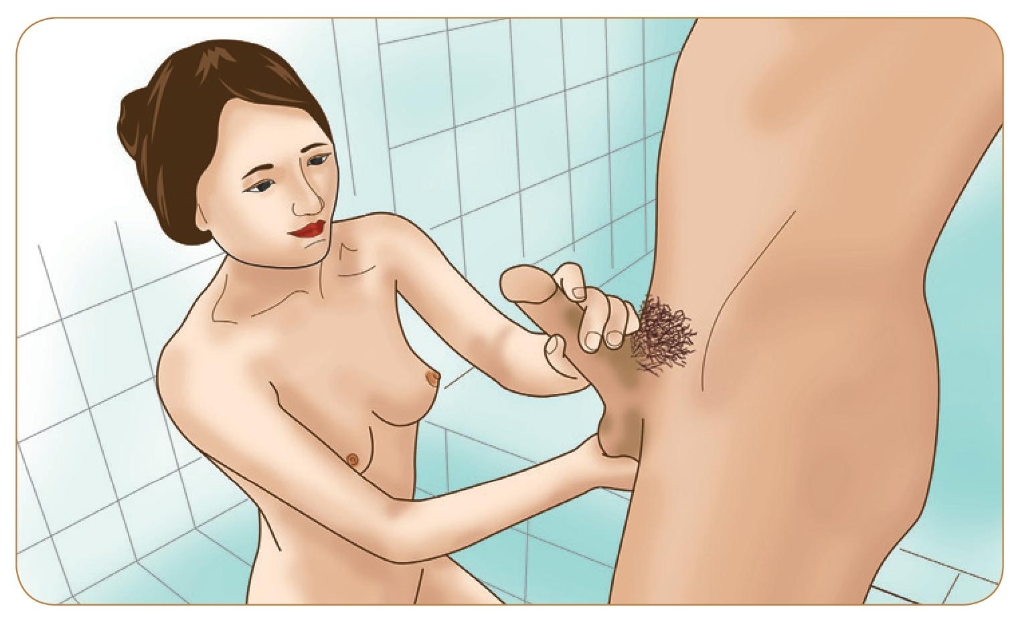
\includegraphics[width=0.7\linewidth]{wf_14.png}
	\caption{女性乳房按摩}
	\label{fig:breast_massage}
\end{figure}

这时，你可以转到他面前，把自
己的乳房抹上滑润的沐浴乳，紧抱
住他，用双乳摩擦男人的胸部，并
且让一支手顺势滑下，男人的阴茎此
刻可能已经勃起，你可以用手指拾起阴
茎，用他的龟头碰触揉搓你的阴蒂、前庭
阴唇，千万要记住，你此刻的心态是在享用男
人，得到性快感，不必单纯只是在討好男人，所以维持多久由你决定!
接下来你可以面对他，蹲下，用手指拎起阴茎，开始含、舔，好似享用
美食一样，反覆舔舐龟头及阴茎干，同时要舔他的阴囊，提醒你，用舌头舔
舐阴囊给男人的快感胜过用口含着龟头，当然，当你把龟头含在口中时，务
必同时用舌头灵巧的绕着舔。
上帝把女人的身体塑造成凹凸有致是有意义的，因为女人好似花朶，
必须藉由芬芳的气味及繽紛的色彩来招蜂引蝶，让男人自投罗网，因此，挑
逗、引誘是女人采取主动性行为的极佳方式!

\begin{figure}[htbp]
	\centering
	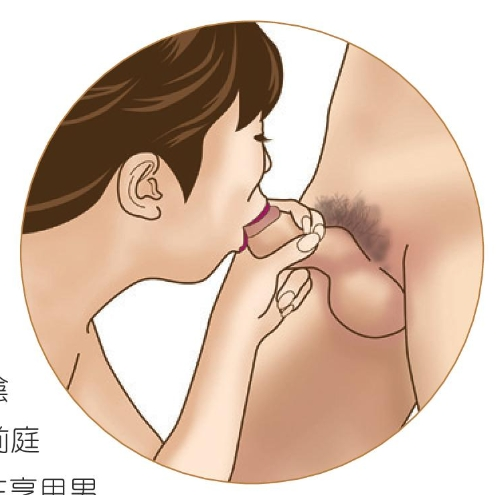
\includegraphics[width=0.7\linewidth]{wf_15.png}
	\caption{女性自慰技巧}
	\label{fig:female_masturbation}
\end{figure}

2.清晨:男人在清晨时分，阴茎常常会自动勃起，这叫“晨勃”，如果前
一天晚上女人想做爱，老公却推托说工作一整天身体很累，那么就让他好好睡上一觉，翌日清晨，你不妨悄悄的把手伸进他的裤裆，让手指有如对待小
寵物般轻抚他的阴茎，很快地，它就会悄悄勃起!
此时你不要只是见獵心喜，要记得先把自己的阴道口及前庭抹上足够的
润滑液，然后用手指托起阴茎，缓缓地坐上去，让阴茎插进你的阴道，在他
半梦半醒之间，两人一起享受一顿丰盛的早餐!但如果男人上午必须要开长
途車或从事重劳务则不宜，否则他很容易因为疲累而在工作时打瞌睡!
挑逗会让男人意识到你的情欲需求，但记得提醒他，满足你的性需求是
他责无旁貸的义务，他必须耗费一部份精神与体力和你共享性爱的欢愉。从
另一个角度看，也让他深深感受到你对他的爱，这样一来，除非他有过人的精力和体力，否则很少会有外溢的力气再
去分享给其他女人。

3.车上:車内的小小空间是两人的
私密園地，也是女人上下其手挑逗彼此
情欲的好地方。通常在男人开車时，你可
以先轻轻地吻一下他的脖子，让他砰然心
动，然后悄悄地将身体靠过去，双手轻轻的拉
下他裤子的拉链，松开他的裤襠，右手缓缓的滑进去，直到你温暖的手轻巧
地握着他迅速膨胀的阴茎，这时，你必须适时提醒他专心开車!随后把你的
头埋在他的双腿间，恣意享用一顿阴茎大餐。
尽管車上的挑逗可以很激情，不过还是要善意的提醒各位:禁止在高速
公路及快速道路上进行，只能在市区及郊区限速50公里以下的道路，且車輛
行駛中只限于口交，如果想替他自慰，务必把車子停在路边，才能避免行車
失控，危害安全，也坏了兴致!

4.野外“偷情”:说是“偷情”，其实是光明正大，但因为是光天化日，
天地无盖，怕人看见，格外紧张，頗有“偷”的气氛，所以用“偷情”来形容。要享受这种乐趣，我建议由你来“偷吃”男人，跳脱在野地让女人局部
卸去衣物，由男人吸吮乳房玩弄私处的传统戏码，你可以让男人背倚着树干
站立，由你解开他的裤襠，掏出他的阴茎，连同睾丸，像老饕享用垂涎已久
的山珍美味般。此刻，男人因为在野外暴露自己的私处，同样会充满着不安
全感，因此能感受到更强烈的刺激，对于你和当下的情景，会永久且深刻地
烙印在他的脑海中!
女人把玩男人的阴茎，用嘴巴、舌头、乳房、手、脚都可以，但是我严
格反对用手替男人自慰!因为男人勃起的每一分一秒都如黄金般宝贵，应该
把它放进你的嘴里或是阴道里尽情享受，如果要让手来，他自己关在厕所就
可以了，某些A片做这样的动作只是表演罷了，千万不能学習!

女人把玩男性的生殖器，对男人来说也是一桩新奇刺激的事。男人过去
一向认为是他主动要求女人宽衣解带，且在他提出需求后女人才会应要求吸
吮他的阳具，如果你采取主动，他会对你有新的认识，会增加日后和你玩性
爱游戏的欲望。
以上几个调情方式供你参考，其实玩弄男人性器官在任何适合的地方、
适当的时间都可以尽情发挥你的创意，譬如在电影院，过去也许是男人主动
伸出手来抚摸你的私密处，现在不妨改由你来出手暗中抚摸他的私密处，他
会既惊訝又兴奋，保证会更加爱你!
除了用手，还可以用脚趾头来挑逗男人的下体!比如在多人聚餐的场
合，如果男伴坐在你的对面，你可以出其不意的脱掉鞋子，伸出右脚在桌面
下用脚趾头去拨弄男伴的下襠，再正视他的表情，对他展现一丝神秘的微
笑，他会巴不得在饭局结束后找你做爱，不信你找机会试试看!
医师的叮嚀:要享受高品质的做爱快感，进而获得极致高潮的快乐，你
做爱时必须心无旁鶩，专心一意地享受当下!

\subsection{女性高潮的多样性}

人们谈论女性的性高潮，一般常会提及“G点”，也就是当触及到女性体
内的这个点，便会让她达到性高潮，但其实不只“G点”，女性体内还有其他
几个地方能有如探触“G点”的效果，来看以下的介紹。

G点高潮(阴道高潮
在阴道前壁约5~7公分处，那个地方就叫“G点”，刺激G点可唤起性高
潮，且会分泌出体液。要怎么找到G点呢？把手指头伸进阴道后再往上勾，会
碰到一块如钱幣大小的皱褶区域，那便是G点，如果碰到G点，高潮便会从那
一点擴散开来。
A点高潮(子宫颈高潮
它的位置在子宫颈跟阴道壁的前穹窿，大概在距离阴道口12公分处。A点
因为比G点更深入、更隐密，且一般男人的阴茎长度不容易到达，也可能因为
做爱时姿势不对，所以A点比较容易被忽略，且A点高潮的特点是只有G点达
到充分高潮后才能找到它。要怎么找到A点呢？如果要自己练习，除非你的手
指头够长，或是透过情趣用品是可以做到的，不过要小心，慢慢来，太过粗
鲁会使阴道前穹窿受伤，若因此造成大出血就麻烦了。
至于什么姿势最能让女伴达到A点高潮呢？

1.女上男下;2.男上，把女生
的腿抬高;3.“传教士”体位。

\begin{figure}[htbp]
	\centering
	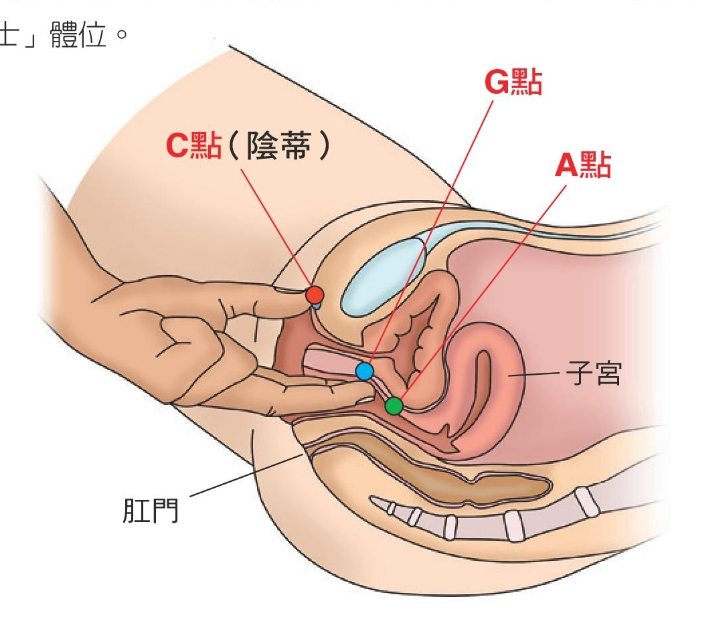
\includegraphics[width=0.7\linewidth]{wf_16.png}
	\caption{传教士体位}
	\label{fig:missionary_position}
\end{figure}

传教士体位(missionary position )
为男性在上面的性交体位，这个称呼源自19世纪，当时的基督教传教
士认为男性在上的体位，是最自然且最适合性交的姿势，这些传教士们也
劝其他国家的信教者，不要使用类似其他动物交配的姿势进行性行为，因
而得名。
此性交姿势是女方平躺，两腿分开且弯曲，男方趴下将阴茎置入女方
阴道，女性可将双脚围绕在男性的背部、臀部，或是举至男性的肩膀，不
同的位置会影响男性阴茎进入的深度。男性可直接趴在女性身上，或是以
手、手肘将身体半支撑起来，或
是采跪坐姿。采这样的体位，男
性可用单臂支撑，空出来的手可
抚摸女性身体，且可尽览女性全
身。以此种体位性交，双方都容
易有性快感。

C点高潮(阴蒂高潮)
根据现代生物学对女性阴蒂的研究显示:阴蒂大约有8千多个神经末梢，
是女性身体里最敏感的组织，要实现阴蒂高潮是很容易做到的。建议刚开始
从内裤外面抚摸就好，中间隔着一层阻隔，先给予适度的刺激;若已经全裸
要直接上阵，可以用按压的方式，揉摸整个阴部以刺激阴蒂，等阴蒂稍微膨
胀后，将手指放在阴蒂上方，轻轻地拨开阴道口，这时阴蒂头的前端会露出
来，只要轻轻抚摸这里，很快就能被快感貫穿。

各个高潮点比一比
G点的神经丛比较多，较容易引起性高潮，以这一点来说，A点高潮
强度的确不如G点。但A点高潮是一种舒缓的愉悦感，不用太大的刺激，还
能有多次的高潮，不像C点高潮是从全身紧繃到放松的感觉，但A点高潮需
要比较深入，对阴茎长度有所限制。女性采坐姿在上位，可补男性阴茎短
的不足，因为采用这个姿势子宫颈可以自动往下碰触男性的阴茎龟头。

\subsection{善用阴蒂享乐}

许多男人都认为阴道是女
性享受性爱乐趣的主要器官，因
为在性爱过程中，男人用勃起的
阴茎插入女性的阴道，这给男人
的印象是“阴道与阴茎是对等
的”，且绝大多数人从小即被教
育:两性的区别在于男人有“小
雞雞”(阴茎)，而女人相对于
男人的身体差异则是阴道。
不论任何文化，在成长过
程中，人们受到的家庭及社会教
育大抵皆是如此，说到女人的性
特征，通常只专注在阴道，阴蒂总是被忽略了!事实上，在性
爱这件事情上，对绝大多数女人
来说，阴蒂才是最主要的感受器官，雖然阴道经常抢走阴蒂的风采，但事实
上，大多数女人初次性高潮是来自阴蒂的自慰!
阴蒂是人体内唯一纯粹以性快感为目的而存在的器官，阴蒂就像男人的
阴茎，不过男人的阴茎兼有排尿的功能。阴蒂又称为“阴核”，雖然它的大
小只像一颗豆子，可说是阴茎的缩小版;埋在包皮里的是“阴蒂柱”，如同
男性包着包皮的阴茎，阴蒂喜欢被触摸，非常敏感，容易兴奋，当女性性兴
奋时，阴蒂柱会迅速膨胀勃起!

阴蒂位在阴道口和尿道之上，构
阴蒂
造与男性阴茎相似，由勃起组织构
尿道
成，头部在小阴唇形成的阴蒂包
皮下突出，柱部则被阴蒂包皮覆
盖，柱体的根部呈左右分开，像
分开的双脚环绕在阴道外侧，并
有肌肉覆盖其上。阴核富有血管
和神经纖维，海绵体亦可膨大，是
女性全身对触觉最敏感的地方，它在
性兴奋及高潮时扮演着重要的角色。
阴蒂柱的根部埋在耻骨前的肌肉里，许多男性以为女性自慰主要是触摸
阴蒂，这是不对的，女人自慰的动作通常是用两至三根手指的指尖揉搓阴核
上部的包皮，先是做绕圆圈的动作，接近高潮时则快速左右揉搓包皮，这个
过程和男人自慰的动作完全一样。
男人自慰是用手指环握着阴茎，快速做上下揉搓的动作，把包皮推到
上方，用包皮揉搓龟头，并以重覆的动作逐渐累积快感，至抵达临界点时射
精，此时能把紧张的情緒完全释放!

女性要享受阴蒂高潮并不是直接用手去碰触阴核头，粉嫩的阴核头露出
在包皮外，因为没有坚实的角质，如果用手指直接触摸，易感觉疼痛，也容
易受伤，所以只能把包皮往前推去碰触，这么做时手指头记得要多抹上一点
润滑液。
“阴核”就是外露的阴蒂头，应该让男人用柔软的舌尖去舔，加上反覆
温柔的按摩，就好像女人帮男人口交时用舌头舔龟头，替男人自慰时用手握
阴茎“柱”，动作为上下推动揉搓包皮是一样的。
大多数女人发现阴蒂并初尝性愉悦，是在青春期从偶然触及阴蒂，或是
在洗澡时用手揉搓时发现的，从此秘境现蹤，在暖暖的被窝里，就不由自主
地把手伸到胯下，开始自慰起来，很多人因此养成无法戒掉的習慣。在寂寞
空虛的夜晚，或是独处的白天，都是行乐的时刻。
有位女士在健康网站问我，她已经养成自慰的習慣，至少两天自娱一
次，结婚半年以来她仍然维持自慰的習慣，她和先生在性交时阴道无法达到
高潮，总是在先生射精后休息睡着时自己再自慰一次。
我建议她和先生沟通，指导先生在性交时可一边抽送阴茎，一边用手轻
揉她的阴蒂，或是她也可以自己用手揉搓阴蒂。经我这么一说，未几时，她
上网欢呼，说她初次尝到了阴道加阴蒂双重高潮的刺激!
医师的叮嚀:每一次做爱，你都不要放棄享受阴蒂高潮的机会!

\begin{figure}[htbp]
	\centering
	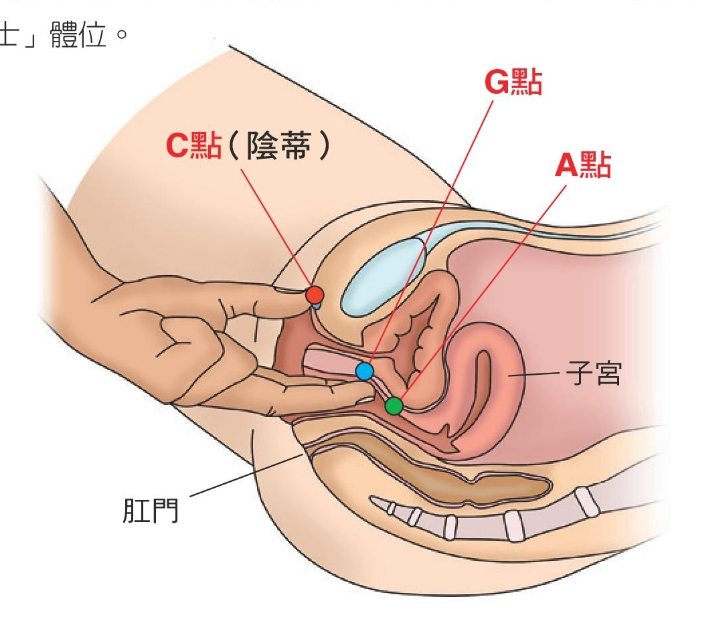
\includegraphics[width=0.7\linewidth]{wf_16.png}
	\caption{女性G点位置}
	\label{fig:g_spot_location}
\end{figure}

\begin{figure}[htbp]
	\centering
	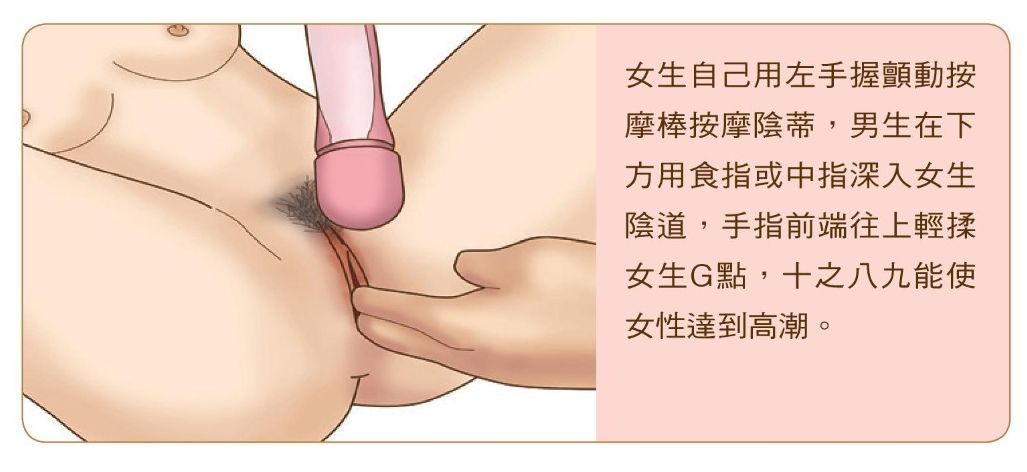
\includegraphics[width=0.7\linewidth]{wf_18.png}
	\caption{男性口交技巧}
	\label{fig:male_oral_technique}
\end{figure}

\subsection{口交技巧详解}

性交当下，主战场当然在阴茎和阴道，主要快感点自然也相同。但我要
教你，在双方性器交合的同时，不要让手和口舌闲着!
女人这一方，当男人俯身抱着你阴茎努力抽送的同时，你可以激情吻他
的颈部和胸部，甚至轻咬，双手可以绕到他背后，以手指轻捏男人的背，适
时表达激情;也可以一手绕到男人背后，轻握并抚摸他的睾丸。

男人这一方，一手务必去爱抚女人的阴蒂，阴蒂绝对是你每次做爱不
能忽略的小宇宙!双唇可不断热吻她的颈、胸、乳头，甚至可以吸吮她的手
指，绝对可以让她很快就欲火焚身!
如果男人在上位，两人身体成90度垂直，则男人可以边抽送边用舌头舔
女人的足踝或是白皙性感的小腿，甚至把她的脚趾头含进口中吸吮，再一手
握她的乳房，轻轻捏住乳头不
要放开，让女人的脚、乳头、
阴道三点同时享受男人的激情
服务。
若女人在上位，坐着推动阴
茎时，一支手一定要绕到背后，
边抚弄男人的睾丸及阴囊，另一
支手的食指及中指则像夾雪茄一
样夾住阴茎的根部，则是阴茎、
阴囊及阴茎根部三处都能同时感
受到刺激!至于舌头呢，可以微
微露出，并发出喘息或惊呼声。

品玉吹簫说口交

“玉”指女性的阴部，“簫”指男性勃起的阴茎，“品玉吹簫”就是指口交。这当然是含蓄的说法，其实，口交是完美性爱很重要的一部份，通常
男人帮女人口交是用来作为性交的前戏，让她兴奋，并接近高潮，或是在男
人高潮射精之前，先让女人达到高潮。或许你没尝试过，或是你没经验过
甜美的口交，想要试试，以下我就来告诉你一场美好的口交儀式需要具备哪
些要件。

1.要慢慢来:性学博士说:“兴奋时，我们的脑袋会变得很猴急，身体
则会生硬地四处乱摸，以满足当下的生理需求。在欲火焚身的时候，我们的
爱抚像单纯的猥亵，欲求不满的亲吻则淪为劣质爱情小说的描写。”也就是
说，男人这时要留意你不安分的身体的所有动作，对女人抚摸要温柔、要到
位，而不是对着胸部、臀部一阵乱抓乱捏。
2.用一点润滑液:借着润滑液的作用，试着让鼻子滑到她的阴部中心，绕
着圈圈在阴唇边缘滚动，或是像点头一样上下前后滑进滑出。深吸气、让自
己自然的发出声音，让她知道你正在享受这个过程。
3.用力吸:将嘴巴张大，盖住她的整个阴部，往外吸的同时把舌头绕圈
转，并且像吸盘那样，把嘴巴营造成一个真空状态，再用点力吸住她的阴部，
最好趁她还没看着你的时候这样做，因为这个动作看起来似乎不是很优雅。
4.轻揉她的私密部位:用一支手掌掌面抵住她的阴部，像揉麵一样轻揉她
的阴部，这时需要借助大量润滑液。
5.用舌尖挑逗:用你的舌尖去挑弄她的阴唇，在她接近高潮的时候，把你
的舌头从阴蒂头直接往下舔到阴唇系带，同时把你的拇指压在她的阴唇上，
这样才有比较多的肌肤表面可以摩擦来产生快感。

大多数伴侣在进行口交时，被服务的一方多半都平躺在床上，这不只限制
了性爱上的深度连结，千篇一律的动作也会让最火热的性事变得无聊。如果你
要改变这种情况，可以尝试布置不同的情境、尝试不同的角色扮演，或是换一
换做爱的地点，女生甚至可以不需宽衣解带，只需脱下内裤，若地点够隐蔽，
随时都可进行。总之，只要用心，一定能激盪出光热交織的性爱火花。

口交实战技巧
按着步驟来，一次就上手:
1.男性慢慢地把头移到女性的双腿间。
2.持续上下亲吻她的阴蒂，这样可引起她的性兴奋。
3.用舌尖轻柔地舔过她的阴阜、阴唇和阴蒂。
4.让舌尖硬挺一些，重复一次舔过她的敏感带。
5.轻轻地吸吮她的阴蒂，用舌尖绕着整个阴部舔。
6.暂停吸吮的动作，用舌面舔舐阴蒂头。
7.交替用唇舌爱抚她的阴部，直到她达到高潮。

\begin{figure}[htbp]
	\centering
	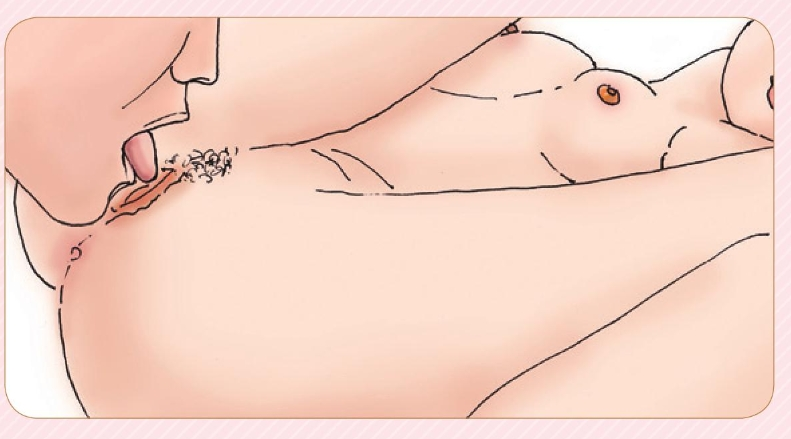
\includegraphics[width=0.7\linewidth]{wf_19.png}
	\caption{女性口交技巧}
	\label{fig:female_oral_technique}
\end{figure}

善用口交技巧征服男人
不像女人的阴蒂只像豆子般大小，
男人的阴茎是一支有温度、可伸缩的
肉棒，吃起来很有口感，握着很有手
感，抚摸很有触感。你可以用嘴把他的
龟头含入口中，像吃棒棒糖一样在口中
滚动，也可以用舌头顺着长长的茎部，从冠
状沟开始，像舔冰棒般来回反覆从包皮舔到根
部，也可以用牙齿轻咬勃起坚硬的阴茎，口感绝佳!如果你要让男人印象更
深刻，不妨口中含着温茶水，再把龟头含入口中，缓缓的漱口，男人的心必
定会感受到你给他的无限温暖。
俗話说，“女人经由满足男人的胃，擄获男人的心”，在现今开放的社
会，这已经不流行了，如今多数女人已经不在家煮饭，所以这句話要改成，
“女人经由口交，擄获男人的心”!
美国前总统柯林顿与白宫实習生李文斯基在白宫椭圆形办公室的口交事
件就是举世皆知的例子;已经退休的美国篮坛巨星迈克尔·乔丹在球赛中场进化妆室时屡次被多名女性冲进去拉下短裤，疯狂争相舔食他的阴茎;歌壇天后麦当
娜甚至在电影“真实与挑战”(Truth or Dare)中秀了一段绝佳口技;某位好
萊塢着名女星也曾公开说她喜爱品尝男人的软屌，“屌”就是男人的阴茎。
可以说，天下男人无不喜爱女人为他们口交，女人们，要收服男人，就
放开心尽情享用男人的阴茎吧!
但我也要提醒女人们，男人胯下的佳餚豈止是阴茎，还有两个像滷蛋的
小菜一一睾丸，也是相当美味可口的。当你要享用时，用拇指及食指把阴茎
往上提起，再用舌头舔遍阴囊，这时你的阴道会不知不觉渗出汨汨的爱液，
而男人在此刻早已神飞九霄!

\begin{figure}[htbp]
	\centering
	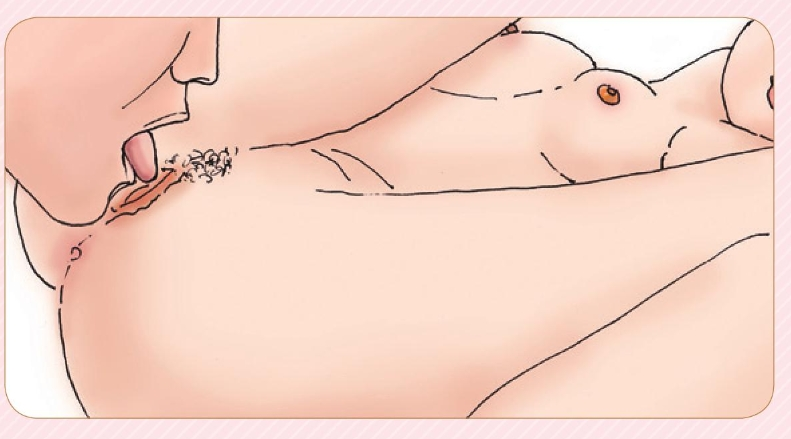
\includegraphics[width=0.7\linewidth]{wf_19.png}
	\caption{男性生殖器口交技巧}
	\label{fig:male_oral_technique_2}
\end{figure}

交可以让女人在做爱这件事上和男人主客位互换，要为他进行口交，
女人甚至可以不脱半件衣物，只要动手解开男人的裤头就可以开始，也不必
局限空间，可以在室内或户外，在浴室洗澡时可以玩，在户外任何角落，如
楼梯间转角、郊外树林中隐蔽处，或是在車上、电影院，只要你把头放低，
埋在男人两腿间即可开动。
趣味小知识
口交算不算性交？
答案是肯定的，口交在法律上算是性交，一方强迫另一方替他口交
算是性侵，而不只是猥亵!若两情相悦而替对方口交就是性交行为。
《史塔报告》透露了美国前总统柯林顿与白宫实習生李文斯基两
人的性关系，包括她多次为这位三军统帥口交的事，柯林顿总统说:
“我没有和那个女人发生性关系!”不过在法律上总统的说法是不成
立的，但该行为若为两愿就不构成犯罪，不过在报告中提到柯林顿想
替李文斯基口交，却因为她当时月经来而被拒绝了，真不凑巧。这个
事件给女人们一个提示:天下男人几乎不会拒绝女人替他口交!
美国没有通姦罪，而我国刑法第10条第5项:称性交者，谓非基
于正当目的所为之下列性侵入行为:1.以性器进入他人之性器、肛门
或口腔，或使之接合之行为。2.以性器以外之其他身体部位或器物进
入他人之性器、肛门，或使之接合之行为。

女人为男人口交这件事完全没有时空限制，不管是在臥房、入住旅店，
当你想要，随时都可以。口交的程序可以由你主动，让男人随你起舞，他绝
对会惊訝且惊喜地拜倒在你灵动的唇舌之下!
女人要主动享受性爱，就从擅用口技、享受口交开始吧!

以下介紹几个常见的口交招式:
嘴唇对阴唇的“传统式”
女人仰臥，两腿张开，建议
用枕头垫高臀部，男人开始轻舔
阴蒂、阴唇、阴道口，接着舌头
伸入阴道浅部伸缩捲绕着舔，这
时你大可闭着眼睛好好享受，但
要提醒你注意以下几件事:
1.专心享受，但要随着男人
舌头转绕自然呻吟、蹙眉，并轻缓的扭动腰身。
2.微微往上挺高你的臀部，就对方的舌头，但是切忌动作太大，否则男人
的舌头会追不上。
3.你必须指引男人舔哪里，力道轻或重，频率快或慢，如果很爽，要高声
惊呼继续，要他舔遍你的阴部!但男人果真认真这样做，不出3分钟，他就会
开始脖子酸痛，脑袋渾沌，如果此时你欲罷不能，不妨用双手扶住他的头，
且把爽叫的音量提高，这对男人有绝佳的激励效果!
4.别让男人的手闲着，提醒男人用食指或中指伸进你的阴道，手指稍微往
上屈，轻抵住G点;或伸入两支手指，中指顶着子宫颈，食指微屈，可触及G
点。

\begin{figure}[htbp]
	\centering
	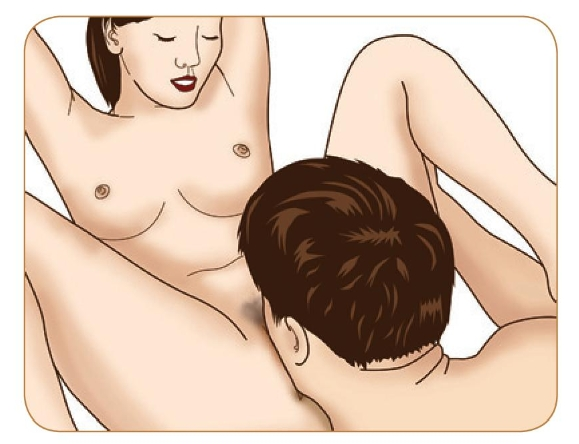
\includegraphics[width=0.7\linewidth]{wf_21.png}
	\caption{性交姿势}
	\label{fig:sexual_position}
\end{figure}

超推荐“骑馬式”
男人躺平，女人面对男
人，跨跪在男人身上，将阴
部对准男人的嘴，男人的头
部最好用小枕头垫高。这叫
“以阴就口”，男人可轻松
恣意品尝美味如生鮮鮑魚的
阴部，这个姿势男人的身体
较不会劳累，所以舌头可以
很灵活的运用，无论阴蒂、
大小阴唇、会阴，都可加长
时间尽情享用，当然，舌头也可不断伸探阴道的深处。
在你尽情享受的同时，男人也别闲着，除了可看着你不断变化表情的
脸，两手别忘向上搓摸你的双乳。

\begin{figure}[htbp]
	\centering
	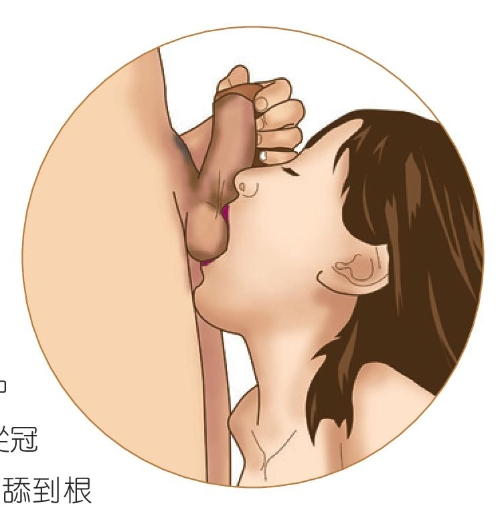
\includegraphics[width=0.7\linewidth]{wf_20.png}
	\caption{性前戏技巧}
	\label{fig:foreplay_techniques}
\end{figure}

床(桌)缘式
日常洗澡后，或是假
日的早晨，女人可以很有情
调的在餐桌舖上浴巾，踩上
椅子，自然地躺在餐桌上，
头舒服地垫着枕头，两脚跨
开，把阴部推向桌缘，男人
抓一把椅子，坐到女人如蘭
花展开的阴部前，用手温柔
的把阴唇向两边掰开，开始
用唇舌大啖宛如无花果的阴部，吸吮它的汁液，轻咬阴唇的嫩肉，好似享用一顿精致早餐!这样做的优
点是男人的颈部不会累，且头部及下巴活动不受限制，想吃多久就吃多久。
若想加点特别的，可巧妙的使用身旁的工具，把奶油、果醬、蜂蜜等塗
在阴部，再用舌头去舔食，可以不停变换口味，随意吃个过瘾!
再次提醒，过程中你务必让呻吟声尽情表露出来，把快乐传进他的心坎
里。

\begin{figure}[htbp]
	\centering
	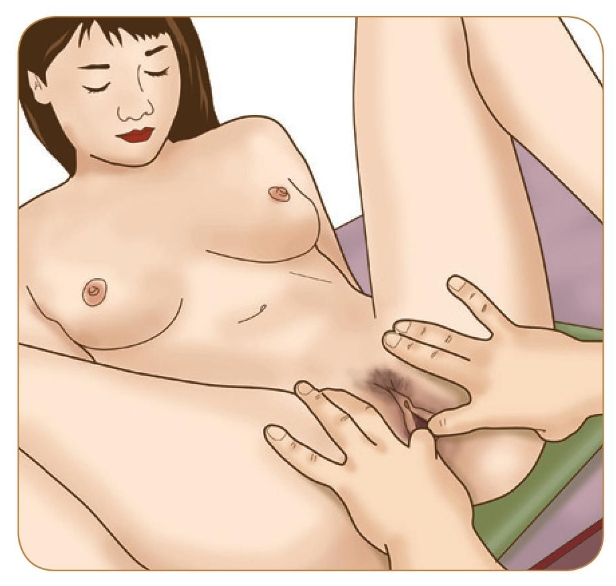
\includegraphics[width=0.7\linewidth]{wf_23.png}
	\caption{女性生殖器结构}
	\label{fig:female_genital_structure}
\end{figure}

早餐菜单加点:
女人站立，上身趴在桌面，两腿张开，让男人把你的底裤拉下，掰开你
的双臀，露出两片可口如淡菜的大小阴唇及樱桃般的阴道小口，加上前端贴
在桌面黝黑如海草的性感阴毛，男人正面坐在矮凳舔食享用，等到女人情欲
高张再高举阴茎插入，享用时别有一番风味。

有问必答
Q:口交会不会传染性病？
A:当然会，而且许多人都是因为
口交而传染上性病。有多种疾病/病原体
都可通过口交传染，如衣原体、梅毒、
淋病、单纯皰疹病毒和HPV等，如果有
以下这些情况，还会增加口腔传染的可
能:牙齦出血、牙齦疾病或口腔健康状
况不佳、口腔溃瘍或生殖器溃瘍等，即
使是受感染的伴侣的尿道球腺液(又名
预射精液)也可能传播疾病，所以，要
避免被传染性病，安全性行为很重要。

Q:自服抗生素能预防性病吗？
A:不能。在现代生活中，一些人受性自由思潮的影响，性行为放纵，但又做"贼"心虚，惧怕性病缠身，往往自作聪明，随意在街头购买一些"大观霉素"、"淋克星"等药滥用，以求自保。结果不但未能预防性病，反而使病情复杂化，甚至出现严重的药物反应，最后不得不到医院求治。

其实每种抗生素都有其有限的抗菌范围（抗菌谱），并非万能神药可以包医百病。由于性病种类繁多，常见的就有十几种，涉及细菌、病毒等七大类微生物，因此，随便选用一种抗生素是无法杀死所有性病病原体的，目前世界上也不存在这样的灵丹妙药。

就拿尖锐湿疣来说吧，它本是一种病毒引起的性病，而街头卖的"淋克星"、"一次灵"等都是些抗细菌的药物，显然不能杀死尖锐湿疣病毒，对其他病毒性性病也毫无作用。

滥用抗生素还会带来以下危害：
1. 容易产生细菌耐药，使治疗康复困难；
2. 容易导致双重感染，出现口腔白斑、念珠菌性肠炎等疾病；
3. 容易出现毒副反应，轻则恶心、呕吐，重则过敏性休克。

自服抗生素不仅不能预防性病，而且会产生不良后果。只有洁身自爱，才是预防性病的正确对策。

Q:自慰会不会引起性病？
A:自慰是所有性行为中最安全的方式，它不会给你带来性病。性生活过度和过滥是两个截然不同的概念，自慰再频也不会患上性病，相反，不安全性交一次也有传染上性病的可能性。

自慰可能会带来一些问题，比如手指摩擦过度造成的或者是阴茎不洁带来的炎症。或者是包皮过长而又经常不洗，造成阴茎有腥臭味黏液。不要为此而担心，可用高锰酸钾溶液浸洗，几日即可消除。

\subparagraph{贴心小叮咛}

自慰不能过频，长此下去，容易造成心理依赖和性功能障碍。自慰动作不能过大过猛，容易造成外伤。

Q:使用避孕套就不会传染性病了吗？
A:很多人以为，戴上避孕套就"安枕无忧"，可以避免染上梅毒、淋病等性病。这种错误认识恰是使自己染上性病，导致蔓延的重要原因。

医学专家指出，作为避孕手段，避孕套若使用正确，基本上可以达到100％的避孕成功率；但若作为预防性病的工具，它的成功率就远不如人们所期待的那样。避孕套对于艾滋病，预防成功率有84％，淋病的成功率只有56％左右，而尖锐湿疣几乎等于零。因为避孕套不是一个"密不透风"的膜，应该说只是一个橡胶网，像精子这些较大的细胞是无法通过的，但是对于支原体、衣原体、细菌等在高倍显微镜下才能看到的很微小的病毒颗粒，它的作用就非常有限了。这就是为什么从事色情行业，或涉足色情场所的人员，几乎都使用了避孕套，而性病仍然无法避免的原因。

因此，预防性病最重要的还是洁身自爱，杜绝不正当的性行为。

\subparagraph{贴心小叮咛}

目前来看，一点细小的失误都会引起麻烦，所以，一定不要以为使用避孕套就不会传染上性病了。

Q:公共场所如何防止传染性传播疾病？
A:有一些性传播疾病的病原体就潜伏在公共场所，比如常见的淋病的病原体淋球菌，适宜在潮湿、温度为35℃和含有2.5％～5.0％二氧化碳的环境中生长，淋菌可在厕所坐垫上或潮湿的毛巾上分别存活18小时和10～24小时。而另一种常见性病——尖锐湿疣的病原体人乳头瘤病毒也可以在适当的条件下存活相当长时间。所以在一些消毒措施不很严格的公共浴池、泳池、美容院或旅馆内，可能接触到沾带性病病原体的物品，如果我们缺乏卫生防病知识，一不小心就能间接染上性病，这种情况在临床上并不少见。

专家认为，虽然淋菌性传播疾病可在公共场所传染，但实际通过接触污染衣物、用具等传染上性传播疾病的机会较少。因此，性传播疾病在公共场所的预防是比较容易做到的。只要我们注意保持衣物、用具的干燥和清洁，创造不利于病原体生存的温度环境，采取必要的预防措施，就能达到预防性传播疾病的目的。

①养成良好的卫生习惯，如上厕所后洗手，勤洗澡、勤换内衣裤；毛巾用后尽量拧干；不使用他人的毛巾、脸盆、浴盆等。

②去公共场所活动时，采取简易有效的隔离措施，如去公共场所使用坐式马桶，尽量不要坐在上面或事先在马桶圈上垫一张纸。去公共浴池洗澡或游泳池游泳，要把自己的衣裤装进自带的袋子、书包或用报纸包好后再放进公共衣柜里。不要把自己的衣服尤其是内衣裤与别人的混放在一起。不要借穿别人的游泳衣和浴衣，也不要光着下身坐在浴室的凳子上。女同志尽量不用浴盆。去旅馆住宿，要检查一下被褥床单等是否干净（多数病菌要在分泌物或脓液中才能存活一段时间），如有分泌物等可请服务员更换。起床后可将被子的被里朝外叠，让其干燥。使用公共浴盆时，要先用肥皂把浴盆刷干净，最好用开水将浴盆全部烫一下再用。送孩子入托最好自带脸盆、毛巾、尿布和被褥等，有条件还可自带尿盆。尿布带回家要用开水烫洗，被褥要勤洗晒。

\subparagraph{贴心小叮咛}

自己孩子的衣物、尿布等要包装在一起，尽量不要与其他孩子的衣物混放或乱穿。

Q:接吻能传染上性病吗？
A:一般人都把"口"当成是人身体器官中相当神圣、尊贵、干净的部位，但事实上，从医学的观点看，人的口腔和肛门是人体细菌最丰富的地方。口腔的血流相当丰富，大部分侵入口腔的病菌很快都会被消灭掉。即使吞食到胃部，很多细菌也难逃胃酸的消毒。这么说来，接吻应该是很安全的！不，一些细菌、病毒还是会成为漏网之鱼，所谓"病从口入"，接吻并不是万无一失的亲密行为。

医学上虽无"热吻症候群"这名词，但在情人节过后，有些人可能会出现颈部淋巴结肿大，全身发热，倦怠，喉咙痛等症状。接吻时如果吸的力道太用力或太久，除了腮帮子的肌肉受牵动，久而出现酸痛现象外，还可能因为口腔内的负压，经由欧式管造成耳内出现闷塞、听力变差或是剧痛的感觉，严重的情形还可能造成急性耳膜破裂。

大部分的流行性感冒都是经由口沫传染。因此在流行性感冒期间，接吻常是病毒感染的最佳媒介，因为即使是嘴唇简单轻碰的接吻都一定会接触到对方微量的口水，很容易就造成感染。

在激烈的拥吻时，如果不小心弄伤了对方口腔或牙龈的黏膜，一定会造成少量的出血，而如果双方都同时受伤，或一方原本就有伤口（最常见的是牙周病），那接吻就不只是口水交流，而是血水交流了，很多原本就藏在血中或唾液中的病菌或病毒就会毫无阻拦地进入对方的身体。

因此除了最常见的感冒外，肝炎、结核病、艾滋病、梅毒、口腔的疱疹等都可能经由接吻的途径感染，因此要和对方深吻前，务必三思。

口交也是性行为中的一种，根据一些民间团体的统计，国内夫妻或情侣有口交行为的占40％以上，而口交正是性病由口腔传染到性器官或反向感染的最佳途径。

本身有流行性感冒，嘴唇口腔疾病（如疱疹）时都不宜接吻，而有梅毒、艾滋病、结核病、肝炎等疾病的人则千万不要和别人有深吻的行为。目前并没有任何的证据显示轻吻艾滋病人的脸颊会因而感染到艾滋病。

\subparagraph{贴心小叮咛}

亲吻或接吻并不是一件随便的行为，因此在你要这么做时，一定要先好好地想过。

Q:消毒润滑剂能防治性病吗？
A:一些专门用于性器官及性生活的消毒润滑剂近年在市场上出现了，有些产品还在说明书上标明"能预防与治疗性病"，因而引起人们的注意。这类消毒润滑剂品牌多，种类也多。可从以下几个方面来谈：从使用对象来区分，可分成男用和女用。男用多为喷雾型，使用时直接喷在外生殖器上，保护一定时间；女用有喷雾型、插入型等多种。从成分上可以分成中药类与西药类两种。中药消毒剂一般由具杀菌或抗菌、消炎等作用的中药组成，作用温和、气味清香；西药类消毒剂的杀菌作用相对地比中药强，另外还含有兴奋与润滑成分。从杀菌作用的强弱来区分，可以分成一般消毒、抗菌、肝炎消毒3类。一般消毒，指只能杀死一般的致病微生物（但对肝炎病毒无效）；所谓抗菌，即只能抑制细菌生长繁殖，而并不能将细菌杀死；肝炎消毒，指能杀死包括肝炎病毒在内的致病微生物。

消除或杀灭外环境中的病原微生物使之达到无害化就称之为消毒，它是作用于体外的病原微生物。毫无疑问，消毒是防治传染病包括性传播疾病的一个重要措施，但是因为任何一种传染病的防治都需要综合性措施，而不是某种单一的措施就可以奏效的。所以消毒并不是唯一与全部，单靠消毒剂是很难达到防治目的的。特别是性传播疾病，要想从根本上预防其发生，只有彻底地杜绝性混乱，这是最根本的。我国曾有一家消毒剂厂商被世界卫生组织判为"无知"，就是因为其厂家出口的消毒剂产品上标有"预防性病"的功效。

消毒剂能治疗性传播疾病这一说法，是无稽之谈。性传播疾病患者绝大多数带有全身症状，而涂于体表的消毒剂只能杀死皮肤黏膜表面的病原微生物，即使是局部的病原体，若存在于皮肤黏膜深层也不能与消毒剂直接接触而被杀死。这样看来，又如何能说消毒剂能治疗性传播疾病呢？对于每一种性传播疾病，我国卫生与世界卫生组织都有一套规定的局部与全身治疗方法，这些绝非消毒剂所能代替的。所以，及时到专科门诊就医，接受正规治疗，这样性传播疾病患者才不会贻误自己的病情。

\subparagraph{贴心小叮咛}

对消毒剂不宜过分强调防治性传播疾病的作用。但是，在性生活前，用合适的清洁消毒剂进行"处理"，可以起到清洁卫生作用，并有可能在一定程度上减少由性交引起的某些感染。

Q:性病患者如何注意自我调养？
A:性病患者由于不知道如何自我调养，最后导致治疗效果不佳，甚至转为慢性，或引起并发症。患性病后应注意以下自我调养方法：

（1）忌口：患性病后，不宜吃辛辣刺激性食品，如辣椒、生姜以及饮浓茶、浓咖啡等。刺激性食品可引起组织充血、加重炎症反应，此外，牛、羊、狗、雄鸡肉也不宜吃。

（2）清心：患性病后，应保持心态平和，切忌怒气冲冲或忧心忡忡。人的情绪与疾病及身体免疫力有很大关系，情绪不好时，人体免疫力下降，易罹患传染病或加重原有疾病的病情。

（3）寡欲：性病未治愈时，应禁止性生活。因性生活会对尿道造成机械性损伤，加重病情。性病传染性很强，性生活会导致性病传播，危害他人健康。

（4）营养：慢性性病患者应注意补充营养。牛奶、蛋、鱼、猪肉、豆制品含丰富的蛋白质及其他营养素，能帮助组织修复，增强身体的免疫力，促进身体恢复。此外，还要注意补充维生素和微量元素。患急性性病时，可服维生素C，因维生素C可增强免疫力和抗炎。

（5）休息：患性病后，应注意休息，切忌过劳，过于劳累导致性病病情加重或复发者，临床上屡见不鲜。急性淋病、非淋、前列腺炎、附睾炎、盆腔炎患者，都宜卧床休息。对于慢性性病患者切忌熬夜、通宵达旦地工作或娱乐，否则会严重影响治疗效果，使疾病迁延不愈。

（6）戒酒：饮酒是性病患者的大忌。饮酒会削弱身体的抵抗力，促使炎症加重和扩散，导致性病转为慢性或引起前列腺炎、附睾炎等并发症。饮酒还是引起性病复发的重要原因。

（7）防病：生病会削弱身体的免疫力，导致原有的性病复发或加重病情。生殖器疱疹、尖锐湿疣等，易在全身或局部炎症的刺激下复发；糖尿病、艾滋病等疾病会加重原有性病病情。

\subparagraph{贴心小叮咛}

反复感染性病，更是将性病推至不治的边缘。因此，患性病后，应注意防病和积极治疗体内其他疾病，特别要注意避免再次感染性病。

Q:为什么性病患者不宜"自我治疗"？
A:通常，人们患了病，都会主动去医院，找医师咨询和求得治疗。然而，一些性病患者，但却不愿去医院，而进行"自我治疗"。其实，这样做是非常有害的。

一些染上性病的患者，囿于羞涩和恐慌心理，不愿主动求医。很多病人凭着侥幸心理，进行"自我治疗"。实践证实，盲目地"自我治疗"非但无效，反而常常是"雪上加霜"。因为患者不了解性病的类型、性质、病情程度，也不懂得采取何种措施才真正有效的情况下进行"自我治疗"，其结果不但延误了诊断时机，也失去了治疗机会。不适当的治疗往往使典型的症状变得不典型，这样就更增加了正确诊断性病的难度，导致性病长期隐匿存在。倘若"自我治疗"中所用药物剂量不当或用错了药，使病菌对真正具有良好疗效的药物产生抗药性，便会增加治疗难度，使所患的性病难以根治。更不可忽视的是，一些不法分子投性病患者所好，兜售假药或变质的药品，"自我治疗"者往往是自投罗网，上当受骗。

所以奉劝性病患者，首先，要停止不洁或淫乱的性行为。其次，要消除羞涩心理，积极、尽快去医院或专门的性病防治机构进行查检和治疗。第三，不要隐瞒病史，应做定期检查。因为某些性病病原体已对药物产生耐药性，所以要较长时间才能观察到预后情况，如梅毒患者要连续观察3年以上。

\subparagraph{贴心小叮咛}

一些不法分子投性病患者所好，专门兜售假药或变质的药品，自我治疗者往往会上当受骗。

Q:性病患者有哪些心理问题？
A:近年来，随着国门的开放，经济的发展，流动人口的增加，一度在我国绝迹的性病又死灰复燃，并迅速蔓延开来。性病患者作为一组特殊的患病人群，不仅具有躯体方面的疾病，由于社会、经济、文化等诸多因素的影响，也产生了一系列特殊的心理问题。这些心理问题的产生与性病的发生、发展密切相关，并影响着性病的治疗、转归及患者愈后的性行为方式。

大多数性病患者存在以下几种心理问题：羞耻感、负罪感、恐惧感、悲观绝望心理、疑病心理、享乐心理、被社会遗弃心理。现代医学认为，疾病不仅发生于器官、细胞上，同样也可引起人的心理状态的改变；反过来，心理因素及社会因素对疾病的发生、发展、转归也有着重要影响。

对性病患者，不仅要治疗其躯体疾病，还要研究其心理特点，了解这些心理特点对治疗、预后可能产生的影响，并帮助其改变不良心态，更好地适应社会。

\subparagraph{贴心小叮咛}

性病治疗要求医生不仅要有高明的医术，而且要掌握心理学的有关知识，在治疗性病的同时，因人而异，针对不同的心理状态施以适当的心理咨询，这样才能收到事半功倍的效果，使性病患者的身心得到完全的康复。

Q:为什么男同性恋者更易患性病？
A:男性同性恋者的性行为方式与正常人的性行为有很大不同，其特殊的性行为更容易招致病毒感染。男性同性恋者之间的性行为主要是肛交，而直肠黏膜上皮比阴道黏膜上皮脆弱得多，很容易造成直肠黏膜损伤。此外，肛门远比阴道狭窄，也容易造成阴茎皮肤的损伤，精液、血液或粪便中的病毒便有可能通过这些微小的损伤相互传播。因此，男性同性恋者之间传播肝炎、艾滋病的可能性比异性恋者大得多。

据有关资料报道，在美国，急性乙型肝炎的发病有21％～23％与同性恋者的性接触有关，尤其与男性同性恋者的性接触有关。男性同性恋者有66.2％的人患过丙型肝炎，其余几种肝炎的发病与传播，男性同性恋行为也是重要的危险因素。

艾滋病的流行与同性恋息息相关。国外一些调查均表明，同性恋者尤其是男性同性恋者，是艾滋病的高危人群；若兼有静脉注射毒品的恶习，则更易招致艾滋病病毒感染。

此外，男性同性恋者大多无固定的性伴侣，性行为混乱，这也是容易招致各种性传播疾病的重要因素。

\subparagraph{贴心小叮咛}

目前，社会对同性恋者的认识已经很宽容，不过为了自己的健康着想，还请三思而慎行。

Q:患艾滋病的妇女可以生育吗？
A:如果法律禁止艾滋病病毒感染者结婚和生育，2010—2030年将使处于生育旺盛期的育龄妇女平均每年减少大约35万人。连同相关因素的影响，我国妇女总的生育率将因此下降大约0.1‰，那么20年间将减少出生人口大约1000万。即便是女性艾滋病病毒感染者结婚生育，由于母婴传播的概率在30％左右，仍有相当一部分婴儿将夭折于艾滋病。

患有艾滋病的病人，不论男性或女性，如果其生殖器官无异常，则不影响受孕。但如母亲患病，可能通过胎盘母婴垂直传播方式感染胎儿，并有可能导致早产及婴儿出生体重降低。母乳也可成为传播的媒介。因此，患艾滋病的妇女不应结婚，更不应妊娠和生育；已婚者应采用避孕措施或实行绝育，已妊娠者应当于妊娠早期施行人工流产，不应继续妊娠，以免使胎儿或新生儿感染此病。

\subparagraph{贴心小叮咛}

如果艾滋病患者坚持要生育自己的宝宝，则一定要在生育前接受专业的医学咨询。

Q:为什么艾滋病关键在于预防？
A:洁身自爱、遵守性道德是预防经性接触感染艾滋病的根本措施。正确使用质量合格的避孕套，及早治疗并治愈性病，可大大减少感染和传播艾滋病、性病的危险。共用注射器静脉吸毒是感染和传播艾滋病的高危险行为，要拒绝毒品，珍爱生命。避免不必要的注射、输血和使用血液制品；必要时，使用经过艾滋病病毒抗体检测合格的血液或血液制品，并使用一次性注射器或经过严格消毒的器具。对感染艾滋病病毒的孕产妇及时采取抗病毒药物干预、减少产时损伤性操作、避免母乳喂养等预防措施，可大大降低胎、婴儿被感染的可能性。艾滋病自愿咨询检测是及早发现感染者和病人的重要防治措施。

\subparagraph{贴心小叮咛}

关心、帮助、不歧视艾滋病病毒感染者和病人，鼓励他们参与艾滋病防治工作，是控制艾滋病传播的重要措施。

Q:艾滋病有什么表现？
A:从感染艾滋病病毒到发病有一个完整的自然过程，临床上将这个过程分为4期：急性感染期、潜伏期、艾滋病前期、典型艾滋病期。不是每个感染者都会完整地出现4期表现，但每个疾病阶段的患者在临床上都可以见到。

\textbf{急性感染期}：窗口期也在这个时间。HIV侵袭人体后对机体的刺激所引起的反应表现为：病人发热、皮疹、淋巴结肿大，还会发生乏力、出汗、恶心、呕吐、腹泻、咽炎等。有的还出现急性无菌性脑膜炎，表现为头痛、神经性症状和脑膜刺激征。急性感染期时，症状常较轻微，容易被忽略。当这种发热等周身不适症状出现后5周左右，血清HIV抗体可呈现阳性反应。

\textbf{潜伏期}：感染者可以没有任何临床症状，但潜伏期不是静止期，更不是安全期，病毒在此期持续繁殖，具有强烈的破坏作用。艾滋病的平均潜伏期，现在认为是2～10年。

\textbf{艾滋病前期}：潜伏期后开始出现与艾滋病有关的症状和体征，直至发展成典型的艾滋病的一段时间。主要的临床表现有：①淋巴结肿大；②全身症状（疲倦无力、周期性低热、夜间盗汗、体重减轻等）；③各种感染（脚癣、尖锐湿疣、口唇单纯疱疹、口腔白色念珠菌感染等）。

\textbf{典型的艾滋病期}：有的学者称其为致死性艾滋病，是艾滋病病毒感染的最终阶段。此期具有3个基本特点：严重的细胞免疫缺陷；发生各种致命性机会性感染；发生各种恶性肿瘤。艾滋病的终期，免疫功能全面崩溃，病人出现各种严重的综合病症，直至死亡。

\subparagraph{贴心小叮咛}

确诊艾滋病不能光靠临床表现，最重要的根据是检查者的血液检测是否为阳性结果，所以怀疑自身感染HIV后应当及时到当地的卫生检疫部门做检查，千万不要自己乱下诊断。

Q:艾滋病是怎样传播的？
A:艾滋病的传播途径有3种：

\textbf{性行为传播}：异性或同性在进行性交、肛交和口交等性行为时，生殖器官的皮肤、黏膜会轻微擦伤，尽管这种擦伤的程度轻微到肉眼看不到，自己也感觉不到，但若一方带有艾滋病病毒，微小的艾滋病病毒就会乘隙而入。这是艾滋病传播的主要途径。

\textbf{血液传播}：共用受艾滋病病毒污染而未消毒的注射器吸毒，使用了受污染又未消毒或消毒不合格的注射器、针头、手术器械、理发刀具，输入含艾滋病病毒的血液、血液制品或器官移植，破损、溃疡的皮肤黏膜接触了含有艾滋病病毒的血液、体液时，都会感染艾滋病病毒。

\textbf{母婴传播}：已受艾滋病病毒感染的孕妇分娩前通过胎盘，分娩时通过产道，分娩后通过哺乳可将艾滋病病毒传播给婴儿。

\subparagraph{贴心小叮咛}

人们与艾滋病病毒感染者或艾滋病病人的日常一般生活和工作接触不会被艾滋病病毒感染，当然也不会得艾滋病。

Q:什么是艾滋病？
A:艾滋病的中文全称是获得性免疫缺陷综合征，英文的缩写是AIDS，中文的音译为艾滋。在香港、台湾地区和海外中文报刊中，也有译为爱滋病、爱之病、爱死病的，意思是本病的发生、传播与人的性行为有密切的关系。

具体些来说，艾滋病是人体自身免疫防卫系统受到破坏的传染性疾病，是由人类免疫缺陷病毒（HIV）侵入人体淋巴系统而致病的，所以它不是一种先天遗传性的疾病，而是后天感染的疾病。患上艾滋病后，免疫防卫功能遭到破坏，人体的抵抗力大大降低乃至完全消失，使得一些病原体或微生物很容易侵入到人体内而致病，而且很难治愈。这些病原体，我们称之为机会感染者，其中有卡氏肺囊虫肺炎、弓形体病、巨细胞病毒、隐孢子虫病、真菌等。作为免疫功能正常的健康人是不容易得这类疾病的，而在免疫功能遭到破坏的艾滋病人身上，这些病原体得到机会，大肆繁殖，构成病态，无法治愈，直至死亡。

2008年12月1日是第21个世界艾滋病日。据卫生部通报，截至9月30日，我国累计报告艾滋病病例264302例；而据卫生部等单位对中国艾滋病疫情的估计，中国现存艾滋病病毒感染者和病人约70万，可能有44万人不知晓自己已经被感染。

最新的调查数据显示，我国部分公众依然歧视艾滋病病人。30％的受访者认为感染了艾滋病的儿童不应该与其他孩子在同所学校学习；接近65％的受访者不愿意与艾滋病感染者同室生活。

卫生部疾控局艾滋病防治处副处长王维真介绍，目前我国艾滋病疫情处于总体低流行、特定人群和局部地区高流行的态势。虽然艾滋病疫情上升速度有所减缓，但性传播已成为主要传播途径。男男同性性行为传播在2005年仅占0.4％，在2007年约占3.3％，感染比例有明显上升趋势。

同时，我国艾滋病疫情的地区分布差异较大。2008年1—9月，共有86.3％的县市区报告了艾滋病病例，报告病例数排行前六位的省份，总病例数约占全国的80％，分别是云南、河南、广西、新疆、广东、四川。

\subparagraph{贴心小叮咛}

2008年我国艾滋病防治工作机制更加健全，全国31个省、自治区、直辖市政府和88％的地州和重点县政府都成立了艾滋病防治领导机构；同时“四免一关怀”政策覆盖面也得到提高。

Q:什么是阴虱病？
A:虱病是虱子引起的皮肤病，世界各地均有发生。阴虱是虱病的一种，可通过性接触传染，常为夫妇共患，而以女性为多见。近年来流行于美国和西欧。

阴虱是长在阴毛根部的一种虱子，使人瘙痒难耐。它常贴伏于皮肤表面，也时常凭其螃蟹样的足爪紧抓阴毛，其卵则可牢固地黏附在阴毛上。皮肤被阴虱叮咬后，可出现高出皮面的红色丘疹，病人感瘙痒，经搔抓往往继发湿疹或毛囊炎。少数病人在股内侧或躯干处还可见蚕豆大至指头大的青灰色或淡青色的青斑，不痒，压之不退色。

\subparagraph{贴心小叮咛}

损害部位常因搔抓损破皮肤组织，继而渗液并形成血痂，可继发为湿疹或毛囊炎等。

Q:怎样识别阴虱？
A:阴虱是一种寄生于人体毛发的寄生虫，长约1～3毫米，无翼。因常见于阴部，故称阴虱。另外，由于阴虱身体扁平，远看如同皮屑，细看则如同小螃蟹，故在英语中又称蟹虱。

阴虱为不完全变态发育，其生活史分为：卵、若虫和成虫3个阶段。

\begin{itemize}
\item \textbf{卵}：阴虱的虫卵一般都紧附在阴毛的毛干根部上，呈淡红色或铁锈色的椭圆形，类似于点状血痂。孵化期约为1周。
\item \textbf{若虫}：若虫是阴虱自卵孵化后，成长为成虫之前的形态。若虫的样子与成虫相似，但是要小很多。若虫的成长期亦为1周。
\item \textbf{成虫}：阴虱的成虫呈灰白色或褐色，雌虫一般比雄虫为大。
\end{itemize}

一般阴虱的寿命是30天，但所有脱离人体的阴虱均会在2天内死亡。

\subparagraph{贴心小叮咛}

若发现阴部有类似的东西，应尽早识别，并加以治疗。

Q:阴虱病怎样防治？
A:阴虱病的防治措施如下：

（1）剃净阴毛及肛周毛发并将其焚烧；
（2）将被污染的衣物、床单、被罩蒸煮或开水浇烫消毒，杀灭虫卵及成虫；
（3）使用热水及肥皂（硫黄皂）清洗阴部；
（4）使用虱立净、百部酊、林旦乳膏、硫黄软膏等涂抹患处，早晚各一次。
（5）由于杀虱剂、林旦乳膏具有神经毒性，且可在体内积聚，因此对孕妇、哺乳期妇女及儿童应避免使用。

\subparagraph{贴心小叮咛}

由于虱虫虫卵孵化需要3～4天的时间，因此治疗期间一定要达到3天，这样可以确保阴虱成虫和虫卵彻底被清除。

Q:生殖器疱疹有什么症状？
A:生殖器疱疹分为原发性与复发性2类。

（1）\textbf{原发性生殖器疱疹}：从感染到发病一般为3～5天，患处先有烧灼感，然后出现红斑，继之在红斑的基础上发生多群红色丘疹，并感到热痒，不久即可变成小水庖，数日后水疱变为脓性，破后可形成糜烂，最后可结痂痊愈。整个病程15～20天。

男性生殖器疱疹，多生于龟头、冠状沟、包皮、阴茎体、尿道口和阴囊。男性同性恋者由于肛交，疱疹可发生于肛门及肛周，严重者可感染直肠。女性好发于大小阴唇、阴阜、阴蒂、阴道等处。男性同时可并发尿道炎、膀胱炎和前列腺炎；女性可并发宫颈炎和子宫炎。大多数患者还可并发双侧腹股沟淋巴结肿大。

（2）\textbf{复发性生殖器疱疹}：大约有60％的原发患者，会在一年内再次复发，第1年至少复发数次，第2年则逐渐减少。复发后一般症状比较轻，也没有淋巴结肿大，病程也短。引起复发的诱因，多为感冒发热、上火、月经来潮、性交过频、疲劳过度、消化不良和气候干燥等。复发时，患处可感到有热刺和痒感。

\subparagraph{贴心小叮咛}

此外，2型疱疹病毒也可使新生儿受到感染。孕妇如在怀孕前3个月感染2型疱疹，有可能会发生胎儿畸形或死胎。如胎儿出生，则可使新生儿受到感染，死亡率可在50％～60％之间。女性如在宫颈、阴部患疱疹，还有发生肿瘤的危险。

Q:生殖器疱疹是怎样的病？
A:生殖器疱疹的发病率很高，在世界上占性传播疾病中的第三位。生殖器疱疹是单纯Ⅱ型病毒引起的，在生殖器发生群集性小疱，糜烂，甚至形成溃疡，可有可无全身症状。

本病发病率高而危害性严重，可引起女性不孕、流产或新生儿死亡，曾患生殖器疱疹的妇女比未患本病者日后发生宫颈癌率高5～10倍，因此许多学者认为宫颈癌和阴茎癌的发病率与生殖器疱疹病毒感染有密切关系，应引起人们对本病的重视。

\subparagraph{贴心小叮咛}

预防生殖器疱疹要避免与发作期生殖器疱疹病人性接触，避孕套不能完全防止病毒的传播。早期妊娠妇女患生殖器疱疹最好中止妊娠，晚期妊娠感染HSV者宜行剖宫产。另外要保持局部卫生清洁。

Q:尖锐湿疣有什么症状？
A:本病潜伏期为3周到8个月，平均3个月左右，由于各人机体对人类乳头瘤病毒抵抗力差异的致病时间长短不一。尖锐湿疣多发生在男女青壮年的外生殖器，肛门周围和肛系带、冠状沟等部，女性多于大小阴唇、阴道、尿道口、会阴部等处，偶尔可出现腋窝、趾间、乳房、脐部等处。损害开始为细小的淡红色丘疹，以后渐渐长大增多，互相融合，重叠隆起，质柔软，表面凹凸不平，呈大小不等的乳头状、蕈状或菜花样，有些似鸡冠花增生，根部有蒂，颜色淡红或污灰，触之易出血。这些疣状物表面湿润，裂缝间常有脓性分泌物淤积，因利于细菌感染而形成糜烂恶臭。患者自觉患部及周围常有不同程度的痒感，常因搔痒抓破而导致继发性感染，并引起附近淋巴结肿大疼痛。

\subparagraph{贴心小叮咛}

尖锐湿疣如不及时、不彻底地治疗，经过一段时间后部分患者可发生癌变。

Q:尖锐湿疣是怎样传染的？
A:尖锐湿疣的传播途径，主要是通过性交直接传染。因性交接触的部位不同而有不同的发病部位，大部分发生于外生殖器，也有肛门周围发病者。在性交时往往皮肤黏膜易发生轻微创伤，这便成了病毒颗粒植入体内的最好门户，感染后平均3个月出现早期损害。首先是上皮局限性增厚，以后呈丝状分裂并渐渐形成乳头瘤样增生，这些损害多在性接触位置上，尤其患淋病和包皮过长的病人，外生殖器长期处于潮湿环境中，更适合生长。

因为非性交因素引起该病的情况比较少见，如通过密切接触污染HPV病毒的毛巾、衣被、浴盆、便器等，也可能发生尖锐湿疣。患有尖锐湿疣的孕妇，在分娩时通过产道传染而引起新生儿喉头疣或呼吸道疣的情况也有报道。

尖锐湿疣的发病，还与身体的免疫机制或抗病能力有关，同样的环境下有的人发病、有的人不发病，或夫妻双方只有一方发病，这种情况即与自身的抗病能力有关。

\subparagraph{贴心小叮咛}

尖锐湿疣本身可以通过药物和手术治疗，但由于目前没有办法从体内将HPV病毒根除，复发的可能性很高，而且终身可以感染别人。感染HPV能提高宫颈癌、直肠癌以及口腔、喉癌的可能性，所以感染者应该经常检查这两种癌症的初期迹象。

Q:软下疳是什么病？
A:软下疳，是由杜克雷嗜血杆菌引起的一种性传播疾病。男性感染后，可在阴茎的龟头、冠状沟、包皮内板、包皮系带等处出现炎症性红斑或丘疹，之后可变成水疱或脓疱，破溃后形成糜烂和溃疡。女性感染后，可在大阴唇、小阴唇、阴蒂，尿道口和会阴部发生病损，其病状和男性相同。除了生殖器病变外，还可发生多处病变，如口唇、手指等处。软下疳的病原体侵入人体后，一般经过2～7天的潜伏期后开始发病。3～8周后，病灶可自行消退。病灶愈合后留有明显瘢痕。

\subparagraph{贴心小叮咛}

过去本病的发病频度在经典性病中次于梅毒和淋病而居第三位，流行于热带和亚热带，在贫困地区、卫生条件不良地方更加猖狂，感染途径是性接触。

Q:患者在治疗非淋菌性尿道炎时应注意什么？
A:患有非淋菌性尿道炎者，在治疗过程中应注意以下几个方面：

（1）由于非淋菌性尿道炎症状不甚典型，时轻时重，尤其是衣原体致病者可持续数月，因此治疗时要排除焦虑心理，积极配合大夫。

（2）治疗前和疗后至少2周禁性交，这样有助于疾病的彻底痊愈。

（3）疗期多饮水，以降低尿的浓度，减轻对尿道的刺激。

（4）不饮酒。饮酒可以加重尿道的充血，使炎症更加急剧。

（5）患者和性伴侣要同时检查，进行正规的治疗。

\subparagraph{贴心小叮咛}

非淋菌性尿道炎的治愈标准为，自觉症状消失，无尿道分泌物，小便沉淀物涂片镜检无白细胞。

Q:非淋菌性尿道炎易出现哪些并发症？
A:患有非淋菌性尿道炎的男女都可出现并发症，男性常见的有附睾炎、前列腺炎、精囊腺炎等，同性恋患者可出现肛门瘙痒和直肠炎。

女性患者较常见的有前庭大腺炎、阴道炎、子宫颈炎、输卵管炎，病原体又可由子宫扩散到腹腔，引起腹膜炎或肝周围炎。这些病人往往出现反复炎症并可造成不育症。

\subparagraph{贴心小叮咛}

对于沙眼衣原体引起的尿道炎患者，即使能生育的妇女，生下来的婴儿也难免因发生眼、耳部的衣原体感染而死亡。

Q:什么是非淋菌性尿道炎？
A:非淋菌性尿道炎简称非淋，是指有尿道炎表现，而分泌物涂片和培养查不到淋球菌的一种泌尿生殖系统感染性疾病。实际致病微生物有沙眼衣原体或解脲支原体等，属常见的性传播疾病，即性病。轻者并发泌尿生殖系统炎症、早泄等疾病，重则直接危害生育功能，导致男性不育。

非淋潜伏期为10～20天。起病症状轻，有尿痛、尿道不适、尿道发痒、烧灼感或刺痛、尿道红肿、尿道有分泌物、稀薄、晨起有"糊口"现象等。随着病情的发展，上述症状将逐渐加重。处理不当或治疗不及时可引起并发症、如急性附睾炎、前列腺炎、结肠炎、不育等疾病。

\subparagraph{贴心小叮咛}

非淋虽然症状较淋病轻，但不像淋病症状常在4～8周自动消失，而是持续时间较长，尤其衣原体原可持续数月之久，且有潜在并发症的可能，必须及时发现及时治疗。

Q:非淋菌性尿道炎有什么症状？
A:非淋主要通过性交传染，沙眼衣原体还可以通过产道传染，引起胎儿的感染。它的潜伏期为1～3周。其临床表现为：

（1）主要表现为尿道炎的症状：尿道刺痒灼痛，可伴轻重不同的尿急、尿痛，尿道红肿，有黏液性分泌物，晨起排尿前尿道口溢液，常污染内裤，以上症状在男性较为明显，女性则症状轻。

（2）男性可合并附睾炎，附睾肿大、发硬且有触痛，有的还可合并睾丸炎、前列腺炎等。

（3）女性可并发输卵管炎、宫颈炎和糜烂、分泌物增多、流产、阴道及外阴瘙痒、盆腔炎、子宫内膜炎、宫外孕及不孕症等。

\subparagraph{贴心小叮咛}

值得注意的是，感染非淋菌性尿道炎的患者中大约有30％～40％在感染后可无明显症状，甚至无症状，容易让患者掉以轻心，失去治疗的最佳时机，从而使治疗非常困难，所以应积极对待。

Q:非淋菌性尿道炎是怎样传染的？
A:非淋主要通过性接触传染，传染源为非淋菌性尿道炎患者和病原体携带者。女性无症状病原体携带者，是最重要的传染源。传染途径包括：

（1）性接触传染：与患者或病原体携带者性接触，可导致传染。性关系紊乱，开始性生活年龄过早，不用避孕套，可使发病率升高。

（2）母婴传染：母亲为病原体感染者，新生儿通过产道时可发生眼部、咽喉、阴部感染，甚至可引起肺炎。

（3）间接传染：通过衣物、用具等可导致传染，尤其多见于儿童。未经严格消毒的妇产科检查器械，也可能成为传播媒介。

\subparagraph{贴心小叮咛}

值得注意的是，患者本人也可通过手或污染物使病原体从生殖道接种到眼睛或咽喉。

Q:淋病患者怎样走出治疗误区？
A:淋病作为我国的第一大性病，其感染人数一直是增长趋势。如何治疗淋病，怎样治疗淋病才能永不复发？不仅是淋病患者非常关心的问题，也是淋病临床治疗需要攻克的关键。要想一次性治愈淋病，必须清楚是什么原因导致淋病复发，这样才能避免走入治疗淋病的误区。

\textbf{用药不合理}

据统计，淋病每天以20％的速度递增传染，这一方面说明了现阶段我国淋病防治工作并没有得到有效的控制，淋病患者治愈率低下这一严重事实；另一方面是得了淋病的很多患者抱有侥幸心理，认为淋病既简单又容易治愈，四处查看淋病的相关知识后，便自行选药治疗，有的服用一些"抗菌药"、"抗生素"等等，经过这样的治疗，淋病患者的表面症状可能会有所好转，症状也会逐渐消失。但是，近年来淋球菌的耐药性愈来愈强，一些诸如青霉素、磺胺药等经不能杀死淋球菌，在患者自行买药治疗或选择其他的仓促治疗后，淋球菌仅仅是得到抑制，并没有被完全消灭，而是潜藏在皮肤黏膜或身体其他部位。几个月之后，不仅可能会转成慢性淋病，而且甚至会引发淋菌性关节炎等其他疾病，这样一来，更加增加了治疗难度，加重了患者的痛苦，最终淋球菌可能通过血行播散至全身，导致严重的全身症状。

\textbf{治疗不彻底}

淋病反复发作，其中治疗不彻底是淋病患者中存在的一个显著问题。一些患者虽然接受过正规治疗，但还是不能杜绝复发，这又是怎么回事？部分淋病患者盲目地认为症状消失便是治愈，往往在治疗两三天后，一看症状逐渐消失，便认为已经治愈了。当然，这和一些医院夸大治疗作用，把价格和时间都定得非常离谱有关。更有甚者有的医院将每日的淋病治疗费用定在400元左右，致使很多患者觉得差不多已经治好，能省既省，没等一个疗程治完就不再就诊了。等到病情又再次发作时，才知后果严重。

\subparagraph{贴心小叮咛}

部分淋病患者求治于街头那些张贴"专治性病"广告的江湖郎中，其实这些游医没有经过专门的学习，使用的又多为伪劣药品，治疗方法极不规范，往往治标不治本，会使病情演变成慢性。

Q:染上淋病何时能与妻子同房？
A:近年来，淋病在我国蔓延很快。淋病主要是通过不洁性生活而传播的。如果经正规专科医师确诊为淋病，在正规疗程结束后的第4天和第8天必须作尿淋球菌涂片和培养。若培养或涂片找到淋球菌，或尿频尿痛、尿道刺痒、尿道口溢脓等症状又出现，则必须重复治疗。

已彻底治愈者，即无症状、培养涂片均阴性的，可同房，但1个月内需用避孕套。因为淋球菌较顽固，房事后易复发。若1个月内无复发，第2个月起可恢复正常房事。

未彻底治愈者，即有尿路刺激症状或涂片培养阳性的，则不宜房事，应继续治疗。另一方面，应作家庭隔离，内裤需烫晒，被、褥、浴具、马桶坐盖等宜分开。

\subparagraph{贴心小叮咛}

患者刚恢复房事，性交后如有复发症状，要及时追加用药，并再做培养。

Q:淋病一定是通过性交传染的吗？
A:提起淋病，一般人都以为只是通过性交传播的，主要表现在生殖器官上，然而近年发现，当人体抵抗力下降时，淋球菌也可通过血液循环在全身播散，医学上称为"播散性淋病"。约0.5％～1％的淋病患者会并发播散性淋病，引起扩散性感染如淋菌性败血症、淋菌性菌血症、淋菌性关节炎、淋菌性心内膜炎、淋菌性脑膜炎等。

例如，有患者手指破损出血后伤口未愈合，当用手指抚摸对方时，对方生殖器官上的淋球菌就通过破损皮肤侵入血液中，最终导致淋菌性关节炎。因此，淋病不一定只通过性交传染，皮肤破损处接触淋球菌也可能导致感染。

\subparagraph{贴心小叮咛}

为了自己及家人的健康，一定要洁身自好，否则会有无穷无尽的麻烦缠着你。

男人舔阴技巧大放送:
女人仰躺在床上，先用小枕头把女生臀部垫高，这样做的好处是可以充分
曝露阴蒂的构造，且男人的脖子比较不会酸，过程可以持久些，方法如下:
1.男人伸出舌头，用舌尖快速左右点触阴蒂，好似电动按摩棒，这会激起
女人快速升高的快感，所以称为“舌尖闪电颤动法”，但是用此法男人最多
持续几分钟舌头就累了，所以要接着做以下的步驟!
2.用舌面由阴道口往上贴着前庭舔到阴蒂，重复进行约1分钟，舌头累了再接下一个步驟。
3.嘴巴张开成魚嘴状，覆盖住整个阴部，用舌头在阴道里左右上下舔阴
蒂，约1分钟。
如此由方法1、2、3循环重覆，两人都不会疲累，直到心满意足。
地点可以随机改变，如女人躺在餐桌上、办公桌上，甚至在户外无人
处，可躺在岩石上、汽車引擎盖上，这样做格外有一种紧张的气氛与情趣!

\subsection{古人的房中术}

古人性爱时的爱抚技巧，是从手指尖到肩
膀，足趾尖到大腿，彼此轻缓地爱抚。脚，先从
大拇趾及第二趾开始，而后逐渐向上游移，这是
因为腿部的末梢神经是由上往下分佈的。指，则
由中指开始，接着是食指与无名指，再是三指交
互摩擦。手，先摩擦手背，而后进入掌心，由掌
心向上游移，用四指在手臂内侧专心爱抚，渐渐
上移至肩膀。
手跟脚的爱抚动作完成后，男人的左手就紧抱女子的脊背，右手再向女子的
阴部爱抚，同时进行接吻。接吻也必须依序渐进，先亲脖子，再亲額头。男人也
可以亲吻对方的喉头、颈部和乳头，并用牙齿轻咬耳朵等女人的性感带。
经过上述程序，充分爱抚女子身体的各主要部位后，再慢慢进行“九浅一
深”或“八浅二深”的交合，双方就能得到十分快感。
俗云:“九浅一深，右三左三，摆若鰻行，进若蛭步。”这几个字说的是:
阳具先浅进九次，使女子春意蕩漾，心猿意馬，然后再做很深入的一进，是谓“九浅一深”。因为在九次浅进时，女子能感受温柔摩擦的快感，然后又受到狠命的一进，心动气颤，男人的龟头直抵阴户深处，
女子即刻陷入极度的兴奋状态，阴道发生反覆膨胀
及不断紧缩的现象。
除了“九浅一深”，阳具还需左冲右突，摩擦
女子阴户右边、左边各三次，此时，女子复又感受
到来自阴道两壁不同的快感，使性欲更是高漲，不
能自己。
男人阳具在进出阴道时，不可呆板地一抽一
送，必须像鰻魚游水，橫向摆动身体，以使女子阴
道两壁都能感受到阳具的冲击。或是在进出阴道
时，采用像蛭蟲走路一般，一上一下拱着身体前进。如此女子的阴道上下壁也能
明显感受到阳具抽插的快感，终而神魂顛倒，乐不可支而达到高潮。
九浅一深也好，八浅二深也好，指的都是性交的韻律，同时限制深入的次
数，除非很特殊的情况，女子才需要每次的插入都直抵阴道最深处，因为每次都
深入这种强烈的快感，极易导致性感知觉麻痺，反而弄巧成拙，且若是过于用力
及次数太多，易使女性感觉疼痛。
《玉房秘诀》、《素女经》，及所有性古籍，都主张男人应尽量理智，延后
射精，以配合女子高潮的到来。这种原则，直到今日仍是医界的一致主张，男性若能按上述方法经常鍛煉，必能增强交合的持续力，使夫妻同登欲望之巔

\subsection{性交礼仪}

性交是一件愉快的事，但如果因为一些琐事坏了兴致，真是会令人扼腕，所以，关于性交的一些基本礼仪，不能不知道。

1.事先征求对方同意。

“女人说不要就是要？”那可不见得。有些大男人几杯黄汤下肚，就强迫老婆或女友配合上床办事，完全不管人家愿不愿意。霸王硬上弓的结果，衍生出许多夫妻间的强暴罪，这属于犯罪行为，因此女生若说不要，最好先判断是真拒绝还是说假的，千万别勉强。

2.不可视为理所当然。

虽说夫妻有同居义务，但若对方无意亲热，就该考量可能是时机不对，不妨花点时间取悦对方，比如，女生可以穿上性感内衣，或者喷点香水，男生可以用音乐、美酒来制造美好气氛，让对方心情好转，两情相悦才能让性爱更甜美。

3.尊重对方。

如果今晚你没有性致，不能拖到上床那一刻才宣布“今天休兵”，要对方紧急刹車，这种沟通方式可能会让对方不高兴。若身体真的不舒服，双方可以思考替代方案，比如以口交或情趣用品等方式来替伴侣宣泄，才不会因床事坏了两人的关系。

4.把身体洗干净。

建议性交前先刷牙、洗澡，尤其双脚应该认真刷洗到没有一丝味道为止，阴道及阴部自不待言，女人该将阴道及外阴都清洗到没味道为止，口臭、汗臭、狐臭也都应该先处理，这是卫生问题，即使是平常，女性的阴部、男性的阳具都应保持干净。

5.使用避孕套。

很多年轻人经常换性伴侣，基于安全性行为考量，在新关系开始的前半年内，从事性行为一定要戴避孕套，因为你无法预知你的新伴侣或对方的旧伴侣有没有性病，所以与新伴侣上床半年内或长期使用避孕套是必需的。

6.在乎对方是否快乐。

性交时不可只顾自己是否达到高潮，却疏忽对方的感受，有些行为粗暴的男生，以为女人在床上的叫声愈大愈愉快，有人为此去入珠，其实那是痛而不快，要真心愉快，两人才能幸福长久。

7.勿苛求对方。

不要因为对方一次表现不好，就给她/他贴上标签，严格要求对方与自己同步产生高潮，这样反而会造成双方的压力，要相互体谅，感情好，高潮自然水到渠成。

8.不要比较性伴侣。

千万不要拿前任男友的床上功夫跟现在的伴侣比较。这是伤感情并损自尊的事，也是非常不礼貌的行为，男性若谨记在心，极可能会产生心因性阳萎，损失的是自己。

9.记得赞美对方。

一场美好的性爱后要记得赞美或道谢，告诉他：“你真的好棒，好厉害！”或“谢谢你让我这么舒服”，适时的赞美可鼓励对方让他的表现愈来愈好。

10.保守性伴侣的秘密。

绝对不要公开性伴侣身上的特征，或对他人谈论自己与性侣伴的私密行为，帮对方维护隐私是成熟人格一定要的，若以炫耀的心态向他人述说伴侣的隐私，只会降低自己的品味，让人对你望之却步。

\section{性敏感部位}
% 移入："敏感区域的爱抚技巧"（本章收解剖与个体差异部分，技巧归"前戏与爱抚"章）
\subsection{男女敏感区分布}

性敏感区的分布有一定规律，但个体差异之大使任何"标准图谱"都只能作为参考。理解一般规律与差异范围，是有效探索的起点。

总体而言，人体的敏感区大致可分为三类。第一类是生殖器区域及其邻近部位，敏感度最高，唤起效应最直接。第二类是次级敏感区，包括乳头、大腿内侧、会阴、臀部、腰骶部、颈侧与耳后等，其唤起效应因人而异但普遍存在。第三类是全身性的皮肤感受，尤其在唤起水平上升后，全身的触觉敏感度会显著提高，此时几乎任何部位的轻柔抚触都可能带来愉悦。

\begin{itemize}
	\item \keyword{生殖器区}：阴蒂、阴茎、阴唇、阴囊等，敏感度最高。
	\item \keyword{次级敏感区}：乳头、大腿内侧、会阴、臀部、腰骶、颈侧、耳后。
	\item \keyword{全身性提升}：唤起后全身触觉敏感度普遍提高，此时期广泛抚触有效。
	\item \keyword{男性忽略区}：男性的乳头、会阴、大腿内侧常被忽略，但同样可能敏感。
\end{itemize}

男性与女性的分布有相似也有差异。相似之处在于，生殖器区域均为核心敏感区，且次级敏感区的分布范围大体一致。差异主要在于：女性的敏感区分布通常更广泛，且唤起更依赖整体情境；男性则相对集中于生殖器区域，且唤起对视觉与直接刺激的反应更快、更直接。这些差异是统计趋势，个别差异往往大于性别差异。

需要强调一个常见现象：随着唤起水平上升，全身的触觉敏感度会提高。这意味着在前戏早期感觉一般的位置，在唤起后可能变得敏感。因此，探索不应局限于固定区域，而应随过程的推进逐步扩展。

\begin{tcolorbox}[colback=pink!5!white,colframe=red!50!black,title=贴心小叮咛]
	所谓"敏感区"，其实会随着状态变化。一开始没什么感觉的地方，也许过一会儿就完全不同了——所以别太早下结论。
\end{tcolorbox}
\subsection{个体差异的范围}

敏感区的个体差异，比多数人想象的更大。理解这一差异的广度，有助于减少自我怀疑与伴侣间的误判。

从分布上看，个体差异体现在几个层面。第一是位置差异：同一区域在不同人身上的敏感度可能天差地别。有人乳头极为敏感，有人完全无感；有人对颈部触碰反应强烈，有人则觉得痒或不适。第二是类型差异：有人偏好轻柔的、缓慢的抚触，有人偏好较强的、明确的压力。第三是情境差异：同一个人的敏感度会随情绪状态、疲劳程度、月经周期、药物使用而变化。

\begin{itemize}
	\item \keyword{位置差异}：同一区域的敏感度在不同人之间差异极大。
	\item \keyword{类型差异}：有人偏好轻缓抚触，有人偏好明确的压力。
	\item \keyword{情境变化}：敏感度随情绪、疲劳、周期与用药状况波动。
	\item \keyword{心理影响}：与某些区域相关的经验或羞耻可显著改变其反应。
	\item \keyword{性别内差异}：个体差异通常大于性别之间的平均差异。
\end{itemize}

心理因素在差异中扮演重要角色。若某个区域与负面经验、羞耻感或创伤记忆相关联，其触碰可能引发不适甚至强烈抗拒；反之，若与正面经验关联，则可能异常敏感。这提示我们：敏感区的分布不是纯生理事实，而是生理与心理经验共同塑造的结果。

实践中最重要的推论是：\keyword{性别之间的平均差异，小于个体之间的差异}。也就是说，"女性喜欢怎样""男性喜欢怎样"这类概括，在具体的人身上往往失效。因此，与其依赖流行知识，不如把每一次互动当作对具体这个人的了解过程——而沟通与观察，是唯一可靠的途径。

\begin{tcolorbox}[colback=pink!5!white,colframe=red!50!black,title=贴心小叮咛]
	“男人都……”“女人都……”这类话，听起来有道理，用起来几乎总是错。你面对的是一个具体的人，不是一整个性别。
\end{tcolorbox}
\subsection{探索与沟通的方法}

探索与沟通是了解彼此敏感区的唯一可靠方法。它们不是可有可无的补充，而是整个过程中最核心的技能。

探索的方法可以归纳为四步。第一，从低压力区域开始：肩背、手臂、腰侧等中性区域的接触，安全且能建立信任。第二，逐步推进：按由外到内、由轻到重的顺序缓慢推进，每一步都留出足够时间。第三，观察反应：留意呼吸变化、肌肉张力、身体的前倾或退缩、以及自发的细微动作与声音。第四，据反馈调整：发现有效的方式就延续，无效或引起不适的立即改变。

\begin{itemize}
	\item \keyword{由外而内}：从低压力区域开始，逐步推进到敏感区域。
	\item \keyword{观察反应}：留意呼吸、肌肉张力、身体的前倾或退缩。
	\item \keyword{简短询问}：以"这样好吗""想要轻一点吗"实时校准，不打断氛围。
	\item \keyword{记录有效}：把有效的部位与方式记住，形成双方的"私有地图"。
	\item \keyword{定期更新}：偏好会随时间变化，不宜以旧有认知替代当下了解。
\end{itemize}

沟通的方法则需要注意形式。在床上进行详细的讨论会打断氛围，因此理想的沟通是简短、即时的——"这样""轻一点""就这样"这类短语即可完成校准。而更详细的讨论（如偏好清单、边界协商）应放在平静的、非性的时段进行，避免在互动中引发压力。

另一个实用的做法是形成"私有地图"。随着时间推移，每对伴侣都会积累一套关于彼此的知识——哪些部位有效、什么力度合适、什么节奏最好。把这套知识有意识地记录与更新，能够显著提高互动效率。但需注意：这份地图是可变的，不应把它固化成"对方一直都喜欢这样"的假设；随着生命阶段、身体状态与心理变化，偏好也会迁移。

\begin{tcolorbox}[colback=pink!5!white,colframe=red!50!black,title=贴心小叮咛]
	每对伴侣最后都会发展出属于自己的一套"地图"。它没法从书上抄，只能一起慢慢画出来——而画的过程，本身就是关系的一部分。
\end{tcolorbox}

人体上有一些特殊的地方，只要一触摸，就能引起很强烈的性愉悦，这些部位就叫作性敏感部位。人人皆知的两个性敏感部位就是乳房和生殖器，除此之外还有许多部位对性刺激反应敏感。对这些部位以刺激，就可以把做爱变成全身参与的活动，而不是一门心思都盯在生殖器官的刺激上。
先从上边说起。许多人喜欢自己的头发被对方揉搓、梳理、亲吻，或者是轻轻拉扯。还有很多人的耳朵比较敏感，他们喜欢对方咬自己的耳垂，对着耳朵轻轻吹气，或者是窃窃私语。后脖颈、嘴唇、乳房周围，还有胳膊内侧、胸脯、腋窝这些地方，不论男女都比较敏感，只要加以抚摸、亲吻，都能引起很大的性愉悦。至于男人的乳头有的敏感，有的不敏感，敏感的就喜欢自己的乳头被啃咬或吮吸，不敏感的则不喜欢这样做。
再往下说。臀部和大腿内侧都是性敏感区域，抚摸、轻啮、玩笑式的掴打，都会使其产生反应。顺着大腿往下，腿弯、小腿、脚踝这些地方也很敏感，凡是玩过在饭桌底下碰人家脚这种把戏的人，都对这一点心知肚明。最后要说到脚和脚趾头，这里是非常有名的性敏感部位——很多人喜欢做足部按摩，喜欢脚趾头被亲吻、吮吸，就是最好的证明。大多数人都知道自己哪个部位最敏感，用什么方法触摸最有效，而只有聪明人才能将这些发现运用到"前戏"的实践当中去。
\subsubsection{人体的性感觉}
人身上的某些器官是专门为生育而存在的，而有些器官的主要作用则是过好性生活。比如，倘若脑部不生产性激素，人的性成熟过程就永远也不能启动。
生殖器官是性快感的焦点。无论是自慰还是性交，只要刺激方法正确，阴道里的肌肉就会出现节律性收缩，让人们享受到性高潮的快感。说到性敏感区域，人们总是会把最大的注意力集中到男女两性的生殖器官以及乳房上，而从某些方面来说，人的全身上下都向外散发着性吸引力，都能强化人的性反应。
除了生殖器官外，人体上的其他部分，如嘴唇等，都有能力唤起人的性欲。人的全身皮肤遍布着上百万个神经末梢，它们对于触摸极为敏感，因此当人们肌肤相亲的时候，就往往会激发出性欲。尽管性高潮时的感觉以生殖器官部位最为强烈，但这种感觉很快就会辐射到全身。
当一个女人达到性高潮时，她的脚背和后背就会弓起来，脚趾头也会出现弯曲，全身的肌肉不自觉地发生收缩，脖子和胸脯上还会布满粉红色的疹子。
人体上的其他部分也能展示出性的魅力。比如阴毛，它是性成熟的标志，还有嘴唇、臀部以及腹部，都充满了性欲的挑动意义。有些人类学家在人体上找到了许多自我摹拟的例子：嘴唇摹拟阴唇，乳房摹拟臀部，肛门摹拟阴道。考虑到人类的祖先是采用后插式体位性交的，这种自我摹拟就显得更有意义了。
\subsubsection{刺激性敏感区域}
长时间地抚摸性敏感区域，不仅可以为做爱搭台唱戏，其本身就是一种性游戏——那种不需要发展到插入的性游戏。
敏感区的分布高度个体化：除阴蒂、阴茎、乳晕等典型区域外，颈后、耳后、手腕内侧、大腿内侧、腰骶部与脚趾之间也常是高回报区。有效的方法不是背清单，而是\textbf{做一轮从头顶到脚趾的"探点"}：用同一手法逐一经过，观察对方的呼吸、肌肉与皮肤反应，再回到反应最强处多停留——\textbf{身体的反馈比任何教程都准确}。
抚摸的要点在于\textbf{慢}与\textbf{专一}：不要把双手当成巡礼的旅人四处游走，而是停留在一处，用指腹、掌心乃至呼吸去体会对方的反应。皮肤在持续、温柔的刺激下，敏感性会逐渐升高——这正是"越抚摸越敏感"的生理基础。同时，抚摸也是一次无声的沟通：对方呼吸变深、身体微微迎向你的手，是在说"就是这样"；而回避或僵硬，则是在请求你换个方式。把这些信号当作地图，比任何"敏感区清单"都更可靠。
\subsubsection{接吻}
嘴唇是人体上最敏感的地方，末梢神经极为丰富。接吻这个动作极富亲密和肉欲的色彩。大量的艺术作品都把接吻作为描绘对象，绘画、雕塑、文学、电影等所有艺术门类都少不了接吻，这一切都足以显示接吻的动人力量。接吻的意义相当宽泛，对于两个新相识者来说，接吻代表着喷薄欲出的激情；而对于一对结婚多年的夫妻来说，接吻则代表着爱情的日常交流。当两个人开始相爱时，接吻常常会成为他们第一次亲密的身体接触。据说当两个人的关系出现恶化时，最早停止的接触就是接吻（甚至要比做爱还早）。
情侣们都知道，接吻并不是一个动作一遍又一遍地反复，两个人仅仅用嘴唇、舌头就能变出很多很多花样来。有不少人发现，把舌头伸到对方的嘴里极具刺激性，轻吻、舔、轻啮这些方式也是如此。实际上，人们所喜爱的接吻方式还有很多，从轻吻到重吻不一而足。
\paragraph{激情拥吻}
接吻是情侣之间用来表达感情最亲密、最富挑逗性的方式之一。激情拥吻往往会成为两个人已经相爱的标志，而结婚多年的夫妻却常常忘记了这种接吻方式。
\paragraph{《箴言集》谈接吻}
《箴言集》一书的作者是印度人，在这本书中他除了对做爱提出了很多有益的忠告外，还列举了大量的接吻方式，其中有直吻、曲吻、回环吻、压吻等等。所谓直吻，就是两个人的嘴唇直接接触到一起；所谓曲吻，就是两个人把头低下，嘴唇靠到一起；所谓回环吻，就是一个人扳住另一个人的头和下巴，把他或她的脸转过来；所谓压吻就是接吻时用力压住对方的下嘴唇。
还有一种法国吻，用作者的话来说就是"舌头之战"。法国吻是紧缠绕吻的一个变种，所谓紧缠绕吻，就是一个人把另一个人的嘴唇全都含在自己嘴里。按照作者的看法，身体上适合接吻部位有前额、眼睛、脸颊、喉咙、胸脯、乳房、嘴唇和口腔内部。
\subsubsection{抚摸}
抚摸是"前戏"的重要组成部分，是爱情与性欲的强烈表现。两个人开始"前戏"时，首先会接吻、触摸脸颊、脖子、头发，接下来就会慢慢地把手挪到肩膀、后背、腹部这样一些地方。动作要特别轻柔，将平放的手掌贴到对方的皮肤上，刚刚碰上就行，即使是抓挠这样的动作，也是用手指尖轻轻地进行。
随着抚摸的进行，重点就会渐渐挪到生殖器官上来，还有可能发生性交，但扔开这一点不论，抚摸本身也非常值得人们去品味一番。从抚摸的定义上说，它不应该是匆匆忙忙的，也不应该引起疼痛或瘙痒的感觉，尤其是在抚摸生殖器官这一带时，这样的感觉更不应该发生。两个人还应该各自把自己喜欢的抚摸方式做给对方看，这样就可以互相抚摸了。
\subsubsection{做爱并非"前戏"的必然结果}
"前戏"的目的在于娱乐、表达爱意、调动性欲。它的下一步可能是做爱，但做爱并不是它的必然结果。按摩、自慰、抚摩都能使人得到与性交一样的满足，但如果你渴望做爱的话，"前戏"就会成为性接触的开端和结束，而当一方想做爱而另一方却不想的时候，这种情况就有必要探讨一下了。
当你因为"前戏"没有发展成做爱而灰心丧气的时候，不妨用温柔亲切的态度向对方提一些问题，鼓励他或她与你一起谈一谈两个人的感受。是不是没有经验造成的？以前你们两个做过爱吗？如果没做过，那就要问一问对方这是不是因为有过什么创伤，还是因为干这种事情负罪感太强烈了？你问过对方喜欢什么样的"前戏"不喜欢什么样的"前戏"没有？你们的关系紧张吗？女方是不是担心或害怕怀孕？是不是男方有早泄，女方有阴道炎之类的难言之隐？会不会是因为从前在这方面有过惨痛的经历？会不会就是因为对做爱不感兴趣或者准备不足？
从另一个方面来说，如果你感觉到对方的性要求比你还迫切，那就要把你不能让对方如意的原因讲清楚。说一说你怎样做舒服，怎样做不舒服，如果你不想跟对方做爱，却乐于帮助对方达到性高潮，也可以说出来。你还可以告诉对方进度太快了，你在心理上还没有做好准备，总之，坦诚的交流可以为你们的性生活设计出完美的蓝图。
\subsubsection{按摩}
按摩不需要什么特殊的技巧，但了解一些简单的要领和基本方法还是必要的。被按摩者要平躺，身下铺的东西要硬一些。按摩者可以分开两腿坐在被按摩者的臀部上，也可以坐在被按摩者的一侧。按摩之前，按摩者要把手涂上按摩油，以保证滑动顺利。按摩开始后，一旦手与皮肤有了接触，就尽可能地不要随便移开。要记住，按摩油对避孕套有损害，所以在做爱前按摩者务必要把手洗干净。
\paragraph{开始按摩}
被按摩者应该把自己愉快的感觉告诉给按摩者。
\paragraph{怎样调制按摩油}
先挑选出一种香精油，茉莉花油、橙花油、薰衣草油、檀香油等均无不可。
用杏仁油或小麦胚芽油等做原油，分别倒进大汤匙里，然后滴进4滴香精油。
搅拌均匀后倒进瓶子里。
每次使用前，将瓶子放进倒入热水的碗里加热，或者用两只手把它搓热。
\paragraph{按摩手法}
\subparagraph{抚法}
手掌平放，做长距离的摩动，此法适合用在身体上面积比较大的地方，比如后背。如果在臀部、肩膀这样的地方施用此法，双手可做短距离移动。
\subparagraph{搓法}
按摩者用两个手掌、手指头或大拇指来挤压、捻动、搓揉被按摩者的皮肉。施用此法可以帮助被按摩者消除肌肉的僵硬，而紧张、忧虑、糟糕的心情都会使这种僵硬的情形加剧。
\subparagraph{摩法}
此法与搓法有些相似，不同的是用的劲要大一些，还可以在原地做旋转揉动，适用于面积比较小的部位。施用此法时，可以用拇指或指关节来增加压力。此法同样有助于消除肌肉的僵硬状态。
\subparagraph{砍法}
按摩者将手掌稍稍成虚拳状，然后实施砍击。也可以将手掌伸直，用掌缘实施砍击。此法可以使被按摩者精神饱满起来，而不会使其精神松弛。
\subsubsection{人体的性感觉}
\subsubsection{刺激性敏感区域}
找敏感区可用"排除法"：先把手掌平放在对方身体上缓慢移动，遇到呼吸变化、肌肉轻微收紧或主动靠过来的位置就标记；一轮之后再逐一回头，用更直接的刺激验证。\textbf{乳头与生殖器之间的神经联系存在明显个体差异}——有人仅靠乳头刺激即可达到高潮，有人则毫无感觉，两种都属正常。
实践中可以给敏感区域排一个大致的顺序：从"外围安全区"（背部、手臂、颈后）开始，逐步向"核心区"（乳房、大腿内侧、外阴）推进，每停留一处都留出足够的时间让对方充分感受。跳跃式地在各处"蜻蜓点水"，反而会让神经系统的兴奋无法累积。此外，不要忽略手指与嘴唇的交替使用——嘴唇的温软与手指的精准相配合，往往比单一工具的持续刺激更有效。
\subsubsection{激情拥吻}
接吻不是前戏的"过场"，它本身就是大量的感觉输入：唇、舌与口腔黏膜密布神经末梢，唾液交换还携带信息素与菌群层面的信息。技巧上常被低估的是\textbf{节奏与呼吸}——先浅后深、有停顿、偶尔后退一两厘米再靠近，比从头到尾同一频率更有效。同时要注意口腔卫生与对方的舒适边界，对刷牙后立即长时间深吻感到不适的人并不少见。
嘴唇与舌尖是人体神经末梢最密集的部位之一，深吻时唤起的不仅是口腔的感受，更是全身的期待。生理层面上，接吻会促进催产素与多巴胺的分泌，带来依恋与愉悦的双重体验；心理层面上，一个投入的吻传递的信息是"我此刻完完全全在你这里"。结婚多年的伴侣不妨有意识地恢复这个习惯——出门前、入睡前的一个长吻，成本极低，却是维系亲密感最省力的投资之一。
\subsubsection{《箴言集》谈接吻}
\section{亲吻与抚摸}
% 移入："亲吻"、"拥抱和抚摸"、"全身抚摸"
\subsection{亲吻的类型与作用}

亲吻是亲密行为中最普遍也最具层次的形式。它有多种类型，各承担不同的功能，远非单一动作。

按亲密程度与功能，可大致分为几类。日常的唇部浅吻（peck）传递的是亲密与确认，是关系中最常规的维系形式；深吻（French kiss）涉及舌部接触，唤起强度较高，是性互动中的常见环节；对颈部、肩胛、耳后的吻则属于探索性亲吻，用于扩大感官刺激的范围；而对身体其他部位的吻（如胸部、腹部、大腿内侧）则常作为前戏的组成部分。

\begin{itemize}
	\item \keyword{浅吻}：唇部轻触，传递亲密与确认，是日常维系的主要形式。
	\item \keyword{深吻}：涉及舌部接触，唤起强度较高，常用于前戏推进。
	\item \keyword{探索性亲吻}：颈部、肩胛、耳后等区域，扩大感官范围。
	\item \keyword{身体亲吻}：其他部位的吻，作为前戏的组成部分。
\end{itemize}

亲吻的作用是多层的。生理层面，嘴唇与舌部神经末梢密集，亲吻能带来直接的感官愉悦，并触发激素相关的反应。心理层面，亲吻是亲密与接纳的直接表达——它传递的"我愿意靠近你"这一信号，对关系中的安全感有实质贡献。研究显示，亲吻的频率与关系满意度之间存在稳定关联。

值得特别指出的是：在长期关系中，亲吻的减少往往先于性频率的下降出现。日常的浅吻是最容易被忙碌挤掉的亲密形式，而它一旦消失，关系往往会逐渐失去"我们仍然是亲密伴侣"这一日常确认。因此，有意识地保留日常的亲吻，是低成本、高回报的关系维护——它的作用虽不如性活动显著，却构成了性亲密的日常基础。

\begin{tcolorbox}[colback=pink!5!white,colframe=red!50!black,title=贴心小叮咛]
	每天出门前那个吻，可能比你们这个月的性生活更能说明你们的关系。别小看它，也别让它悄悄消失。
\end{tcolorbox}
\subsection{全身抚摸的顺序}

全身抚摸的顺序，是前戏技术中一个具体而实用的议题。合理的顺序能最大化唤起效果，而错误的顺序往往导致体验不佳。

基本顺序遵循"由外而内、由轻而重、由非敏感而敏感"的原则。具体而言：从背部、肩颈、手臂等中性区域开始；逐步移向腰侧、腹部、胸部等次级敏感区；然后是大腿内侧、臀部等靠近生殖器的区域；最后才进入生殖器区域。这一顺序的意义在于：唤起需要时间积累，而大范围的体表刺激本身就是有效的唤起途径。

\begin{itemize}
	\item \keyword{中性区域起}：背部、肩颈、手臂，建立接触与放松。
	\item \keyword{次级敏感区}：腰侧、腹部、胸部，逐步提升唤起。
	\item \keyword{邻近区域}：大腿内侧、臀部，营造期待感。
	\item \keyword{生殖器区域}：最后进入，且从轻柔开始。
	\item \keyword{回环往复}：不必线性推进，可反复回到先前的区域。
\end{itemize}

需要补充两点。第一，顺序不是单程路线。有效的做法是"回环往复"——在推进到某一区域后，可以回到先前的区域重新刺激，再推进。这种往复能避免线性推进带来的"过了就没了"的压力，也使过程更松弛、更持久。

第二，顺序应依对方反应而调整。若在某一区域获得明显反应，宜在此多停留；若某区域引起不适或无明显反应，可以缩短或跳过。此外，需要注意：当唤起上升后，全身的触觉敏感度会普遍提高，此时先前的"中性区域"也可能变得敏感有效。因此，顺序的核心不是固定的路线图，而是"由外而内"这一方向性原则。

\begin{tcolorbox}[colback=pink!5!white,colframe=red!50!black,title=贴心小叮咛]
	别把顺序当成一条必须走完的路线。什么时候往前、什么时候往回，看的是对方的反应，而不是你心里那张图。
\end{tcolorbox}
\subsection{力度与节奏}

力度与节奏是抚摸技术中两个最关键、也最难以言传的变量。它们共同决定了体验的质感。

力度方面，基本原则是"宁轻勿重"。多数人对过强的力度会产生不适而非愉悦，尤其在敏感区域。轻的力度还有一个优势：它可以通过增加时长与稳定性来积累效果，而不必依赖强度。实践中的典型错误就是力度过大——尤其在急于推进时，手上会不自觉地加力。

\begin{itemize}
	\item \keyword{宁轻勿重}：从轻开始，逐步调整，避免一开始就用力。
	\item \keyword{区分部位}：肌肉丰厚处可用较大力度，敏感区需大幅减轻。
	\item \keyword{节奏变化}：快慢交替、适时停顿，避免单一节奏的适应。
	\item \keyword{稳定积累}：接近高潮时保持稳定节奏，比突然加速更有效。
	\item \keyword{手温指甲}：手部温暖、指甲修剪，是基础的舒适前提。
\end{itemize}

节奏方面，核心是"变化"与"稳定"的合理运用。在唤起上升期，变化（快慢交替、强弱交替、适时停顿）能有效维持兴奋水平，避免感觉适应。但在接近高潮的阶段，多数人需要一段稳定、持续的刺激积累，此时突然的变化可能打断进展。因此，"何时变化"比"是否变化"更需要判断，而判断的唯一依据是对方的实时反馈。

除力度与节奏之外，还有两个常被忽略的细节。第一是手部温度：冰凉的手会造成明显不适，尤其在敏感区域，事先搓热双手或在温水中浸泡是简单有效的准备。第二是指甲：过长的指甲容易造成划伤，而这类微小的伤口在敏感区域可能引起感染或持续不适。这些细节看似琐碎，却直接影响体验。

\begin{tcolorbox}[colback=pink!5!white,colframe=red!50!black,title=贴心小叮咛]
	两只手，记得要先搓热。这个动作花不了三秒钟，但它决定了对方的第一感受是舒服还是被吓一跳。
\end{tcolorbox}


\section{性生活的前奏曲}
% ⇒ [r81 并入] 自旧区
大家在前戏中会做什么样的爱抚呢？

前戏和插入，到底哪个对性爱来说更重要呢？

答案显而易见。如果从女性的快感与满足感这个角度来考虑的话，那就是前戏。在面向读者的新闻网站、女性杂志的问卷调查中，都有类似的调查，根据这些调查的结果，女性回答"人生最低的性爱"时，"男性的自以为是式性爱"和"没有前戏的性爱"占了大多数。

所谓"自以为是的性爱"，是指对女性的体贴不足。例如，女性明明不愿意却强行肛交、女性完全没有兴趣却被言语责骂、明明感觉到女性在痛却误以为是她享受而用力冲刺……这些都是男性随自己的欲望去做的案例。也有女性因为被强行无套插入而在整个做爱过程中一直担心怀孕。一部分男性之所以会这样做，成人视频（AV）的影响不可否认。现代AV作品多以男性性幻想的最大公约数来制作，不过是男性单方面需求的"性脚本"——在这种"幻想"中，女性按照男性的剧本反应，但现实中的女性并不接受这样的节奏和方式。

许多男性声称"我懂那种事"或"我才不会做像AV那样只顾自己舒服的性爱"，大家都想给女性最好的体验，想进行让女性最舒服的性爱，这应该都是普遍的想法。但关于"没有前戏的性爱"又是怎样的呢？接吻、轻轻揉胸、确认性器已经湿润后，是否马上就插入？如果前戏时间不足，那么和"自以为是的性爱"几乎一样，都会被女性评价为最糟糕的性爱。

很多男性为了满足女性器官，在过程中进行爱抚，把性高潮的顶点（climax）理解为插入或射精，这样好吗？从生物学角度来说，男性的性行为是在女性阴道内射精、留下后代的行为，这种想法当然有其道理。这对女性来说也是如此。留下后代是重要的生物学使命。然而，不能因此就认为女性的性欲比男性弱，更不能让她们处于不得不假装高潮来取悦对方的境地。否则，那反而会引起对性的厌恶心理。

男性通过睾酮等雄激素刺激大脑唤起性兴奋，而女性则无法停止大脑的一部分活动，因此无法唤起性兴奋。掌管不安和恐惧情绪的扁桃体倾向于将性的冲动几乎完全置于控制之下。总之，即使女性的性兴奋被激发，也无法构建单纯的结构来实现射精。

那么，是不是说当女性被情欲点燃时，就无法将性兴奋推向更高了呢？

答案是否定的。绝非如此。女性本能地追求快感、渴望男性。然而，如果不能在瞬间将性兴奋推向高潮，男女之间的差异就会导致性被绕过、勉强凑合的情况发生。对女性来说，性生活中真正需要的不是谁都会喜欢的某种形象，也不是成人视频里那种夸张的姿势。女性所渴望的是从不安和恐惧中解脱出来的安心感以及由此带来的快感。如果没有信赖感，就无法唤醒沉睡于女性心底的炽热高潮。这种安心感和信赖需要通过行动来展示——这就是前戏的作用。为了让女性达到极致的高潮，充分的前戏是不可或缺的。通过前戏，让女性从内心深处感到满足和幸福、沉浸在幸福氛围之中——这正是本书要讲解的种种前戏技巧的目的所在。\hfill \textit{——铃木享治，《Maniaxクラブ研究会》}

做爱开始前两个人为唤起性欲而做的所有事情都可以称为"前戏"。它包括接吻、拥抱、轻轻的啃咬、相互抚摸、按揉乳房和生殖器官、性按摩、口交和助兴用品的使用。

\subsection{宽衣解带}

两个人上床之前，就应该做些准备了。许多夫妻喜欢先一起洗个澡，或者是互相脱衣服。

所谓前戏，就是让身体处于做爱的最佳状态。随着接吻、拥抱、相互抚摸的进行，两个人的情绪逐渐调动起来了，其肉体也为插入做好了准备（"前戏"的最终结果并不一定就是做爱）。男人的阴茎开始勃起，女人的阴道开始变深，同时分泌出润滑液体，阴道壁变厚，阴道口变大，这一切都为了方便阴茎的插入。一般来说，女性的性兴奋状态要比男人来得慢一些，所以"前戏"对女人来说就显得更重要一些，尤其是那些需要足够的刺激才能达到性高潮的女性，"前戏"的意义更是非同小可。

"前戏"还可以帮助两个人从容不迫地享受那种肉体相挨，心灵相契的亲密感觉。性的交合需要两颗心的坦白、信任和容纳，而"前戏"恰恰可以把两个人送进这样的境界之中。

\subsection{环境的重要性}

对于亲密的性接触来说，好的环境是很重要的。首先一点是要有保密性，两个人要约定好，听到敲门声谁也不答应、响起了电话铃声也不去接。尽管不同的地方有不同的要求和习惯，但个人卫生还是应该尽量搞好，一般来说至少应该刷刷牙，洗洗头，有条件时还应该洗个澡，特别需要注意的是，要把腋窝、脚、生殖器这些地方洗干净。许多人发现，一起洗澡或淋浴对双方的心情都有很好的放松作用。如果能事先在洗澡水里加入一点芳香剂，效果那就更好了。一边洗澡一边帮着对方洗洗头，或者先将带香味的洗剂涂抹到对方身上，再按摩按摩，彼此的亲近感就会油然而生。索性就在浴室里做爱，也会令人很兴奋。

做爱之前把房间收拾一下，让音响里放出轻柔的音乐，亮起幽暗的灯光（或者点上蜡烛），贴上撩拨人心神的图片，打开香水瓶任其挥发，点上香让香烟缭绕，还不要忘记摆上鲜花，如此等等都可以有利于创造适合做爱的良好氛围。

\subsection{还是要慢慢来}

一个人有一个人所常用的"前戏"方式。有的人喜欢悠着来，不紧不慢的，什么方法都尝试尝试，等到再也拖不下去的时候才插入。在这种情况里，"前戏"的主要作用就在于循序渐进地把人带进最后的性兴奋中。而有些人却不是这样，他们的性兴奋来得很快，容不得你有什么准备就把事儿干完了。还有一些人花在"前戏"上的时间很长，只有这样才能进入性交，而对于这种人来说，"前戏"就变得与做爱本身一样重要了。

那么，前戏到底需要多长时间呢？根据面向女性读者的调查问卷显示，女性对前戏的理想时间要求几乎都是"10分钟以上"。相反，如果前戏时间低于10分钟，超过八成的女性会感到"最糟糕"。相对于男性只顾追求射精的快感而冲刺，女性比起匆忙达到高潮，更重视花时间享受充实的性爱。从生理上来说，如果女性性器官没有充分湿润，插入时会伴随疼痛——这一点也不快乐。花足够的时间，不仅让身体充分准备好，更能消除女性的不安感，这正是高质量前戏的关键所在。

\subsection{暗示的作用}

大凡性事，朦胧的东西最妙——惊鸿一现总比一览无余更能令人心醉神迷。情欲高涨之时，七手八脚地扯去对方的衣服，确实特别刺激；而在有些时候，让对方的肉体慢慢地、一点一点地裸露出来，会显得更具诱惑力。很多人发现，最能激发性欲的方法不是一上来就直奔乳房或生殖器官刺激而去，而是轻柔地触摸大腿、臀部、脚这样一些比较微妙的性敏感部位。

各种暗示也可以用来引发性兴奋。只要能让对方产生亲密接触的意识或心情，"前戏"的作用也就达到了。比如，从外地打来一个电话，或者写来一封信，暗示自己有那种想法，就可以源源不断地点燃对方的情欲。不管两个人如何走到一起的，如果能共进一顿浪漫的晚餐，或者是到郊外散散步，就可能自然而然地睡到一起。还有做爱之前长时间的接吻、抚摸、触碰，也都能引起性兴奋。暗示这个小把戏甚至可以用到触摸性器官上来，比如女方用手轻柔地握住男方的生殖器，却不做什么动作，可男方就已经明了她的心意了。

\subsection{全身抚摸}

亲吻、舔、啃咬、抚摸性敏感区域，能够极大地提升双方的性兴奋程度。在做爱的准备阶段里，脚趾、腿弯、手指头、眼皮这些地方常常被忽视。而如果能对这些部位施以缓慢而足够的性刺激，相信很多人都能从中获得新奇的体验。


全身抚摸的价值在于把注意力从"目标器官"移开。建议先由接收方说明偏好：是希望轻若羽毛的划触，还是希望带压力的揉按；用什么速度、避开哪些区域（腰侧、脚底、颈侧常是怕痒或敏感的重灾区）。施予者可用指尖、掌根、前臂轮换，并注意\textbf{手温}——冰凉的双手会让肌肉瞬间收紧。全程保留"可以随时喊停"的约定，抚摸才可能从"前戏任务"变成真正让人放松的接触。

关于前戏，有几点常被忽视的要点值得补充。首先，"前戏"并不等于机械的流程清单——接吻、抚摸之所以有效，是因为它们传递了"我渴望你、我在意你的感受"的信息；脱离了情感投入，任何技巧都会显得空洞。其次，前戏的长度没有标准答案：研究显示伴侣双方对理想时长的估计常常相差数倍，与其对照"平均数"，不如以双方的生理信号（润滑充分、勃起稳定、呼吸与肌肉的放松）和心理感受为准。第三，前戏也是安全性行为的一部分——戴上避孕套、检查玩具清洁、确认彼此的意愿边界，都属于"开始之前"该完成的事。对老年伴侣、产后女性或使用药物的人群，充分的前戏还能弥补润滑不足与唤起迟缓，是提升舒适度的第一手段。
\subsection{宽衣解带}
对于亲密的性接触来说，好的环境也是很重要的。首先一点是要有保密性，两个人要约定好，听到敲门声谁也不答应，响起了电话铃声也不去接。尽管不同的地方有不同的要求和习惯，但个人卫生还是应该尽量搞好，一般来说至少应该刷刷牙，洗洗头，有条件时还应该洗个澡，特别需要注意的是，要把腋窝、脚、生殖器这些地方洗干净。许多人发现，一起洗澡或淋浴对双方的心情都有很好的放松作用。如果能事先在洗澡水里加入一点芳香剂，效果那就更好了。一边洗澡一边帮对方洗洗头，或者先将带香味的洗剂涂抹到对方身上，再按摩按摩，彼此的亲近感就会油然而生。索性就在浴室里做爱，也会令人很兴奋。
做爱之前把房间收拾一下，让音响里放出轻柔的音乐，亮起幽暗的灯光（或者点上蜡烛），贴上撩拨人心神的图片，打开香水瓶任其挥发，点上香让香烟缭绕，还要不要忘记摆上鲜花，如此等等都可以有利于创造适合做爱的良好氛围。
\subsection{还是要慢慢来}
性活动最容易被忽略的建议就是"慢"。绝大多数首次体验不佳、出血与疼痛，都与节奏过快有关。可行做法：先把"插入"从时间轴上暂时去掉，用半小时只做接触与抚摸；进入时采取浅、慢、随时可停的节律，让身体有几十秒到几分钟的适应期；\textbf{任何刺痛都不是"忍一忍就过去"的信号，而是需要换节奏或加润滑的提示}。
\subsection{暗示的作用}
\subsection{全身抚摸}
此处的全身抚摸更强调技法顺序：一般从远离生殖器的部位开始（肩、背、手臂、小腿），逐渐向躯干与大腿内侧靠近，最后才到生殖器，使紧张逐层卸下。手法上可用"三速轮换"——极慢的划触、中速的掌压、微快的揉搓——每隔一两分钟切换一次，避免身体对单一刺激产生适应。\textbf{当对方开始不自觉地配合动作、呼吸变深，通常说明已进入状态。}

\section{前戏技巧}
% ⇒ [r81 并入] 自旧区
前戏是指性行为开始前的亲密接触和刺激，是性生活中不可或缺的重要环节。研究表明，充分的前戏可以提高女性达到性高潮的概率，从平均30%提高到70%以上(2022年《女性性健康杂志》)。


前戏技巧的核心是\textbf{把唤起当作需要积累的过程而非开关}：一般建议先做与生殖器无关的接触（交谈、亲吻、拥抱、背部与四肢的抚摸）以降低紧张，再逐步过渡到敏感区域，并允许节奏反复（可以变慢、可以停下、可以倒退一步）。\textbf{两个具体的技术要点}：一是\textbf{润滑的使用不被视为"准备不足"}（它是提高舒适度最直接的工具，尤其对产后、哺乳期与绝经后的女性）；二是\textbf{不要在临近高潮时突然切换方式}（打乱即将达成的节律往往会让积累归零）。

\subsection{前戏的生理与心理作用}

从生理学角度来看，前戏可以：
1. \textbf{促进性唤起}：通过刺激敏感区域，促进血液流向生殖器官，增加阴道润滑，为性交做好准备。
2. \textbf{缓解紧张情绪}：减轻压力和焦虑，帮助伴侣放松身心，增强性体验。
3. \textbf{增强情感连接}：通过亲密接触，释放催产素等"爱情激素"，增强伴侣之间的情感纽带。

\subsection{有效的前戏技巧}

\subsubsection{身体接触与抚摸}
\begin{itemize}
\item \textbf{温柔抚摸}：从非敏感区域开始，如手臂、背部、颈部，逐渐过渡到性敏感区域。
\item \textbf{亲吻技巧}：亲吻不仅局限于嘴唇，可以尝试亲吻颈部、耳朵、胸部等敏感部位。
\item \textbf{拥抱与依偎}：亲密的拥抱和依偎可以增加情感连接，为后续的性活动奠定基础。
\end{itemize}

\subsubsection{性敏感区域的刺激}

根据2023年性学研究，人体有多个性敏感区域：
1. \textbf{主要性敏感区域}：阴蒂、阴茎、乳头等。
2. \textbf{次要性敏感区域}：耳朵、颈部、大腿内侧、臀部等。

\paragraph{技巧提示}
\begin{itemize}
\item 刺激阴蒂时，使用温柔的触摸，可以用手指轻轻环绕阴蒂，避免直接强烈刺激。
\item 刺激乳头时，注意力度和节奏，可以交替使用轻触、吸吮等方式。
\end{itemize}

\subsubsection{沟通与反馈}

前戏过程中，伴侣之间的沟通至关重要。可以通过语言或非语言信号(如呻吟、身体姿势变化)来表达自己的感受和需求。


沟通与反馈在技巧层面的具体化就是三句话：\textbf{"我喜欢……"}（指出有效的方式，帮助对方建立准确的操作模型）；\textbf{"轻一点、慢一点、换个位置"}（在过程中即时微调，而不是事后总结）；\textbf{"现在这样很好"}（正向反馈能显著降低对方的焦虑，而焦虑正是表现失常的主要来源）。\textbf{需要避免的两种表达}：一是把不满包装成对人格的评价（"你怎么总是这样"）；二是完全沉默地忍受不适（这会同时损害体验与身体安全）。

\chapter{前戏中的生理反应与高潮铺垫}
\section{呼吸、吟叫与身体扭动}
\section{女性高潮的多样性}
% 移入："女性高潮的多样性"、"善用阴蒂享乐"
\subsection{阴蒂的解剖与功能}

阴蒂（clitoris）是女性性解剖中最重要却长期被误解的器官。它的唯一已知功能是提供性愉悦，其神经分布之密集在人体中极为突出。

解剖上，阴蒂由可见的阴蒂头（glans clitoris）与大部分位于体内的结构组成。阴蒂头位于小阴唇前端交汇处，被阴蒂包皮部分覆盖；体内部分包括阴蒂体与阴蒂脚（crura），向两侧延伸并环绕阴道开口，总长度可达数厘米。因此，所谓"阴蒂"远不止外部可见的小突起，而是一个具有内部延伸的立体结构。

\begin{itemize}
  \item \keyword{阴蒂头}：外部可见部分，神经末梢极为密集，敏感度最高。
  \item \keyword{阴蒂包皮}：覆盖阴蒂头的组织，其覆盖程度因人而异。
  \item \keyword{阴蒂脚}：向体内两侧延伸的部分，环绕阴道开口周围。
  \item \keyword{前庭球}：与阴蒂相邻的充血组织，唤起时明显肿胀。
  \item \keyword{神经分布}：阴蒂的神经末梢密度远高于其他性器官区域。
\end{itemize}

功能上，阴蒂是女性性愉悦的主要来源。研究反复显示，多数女性需要阴蒂区域的刺激才能达到高潮，单纯阴道性交往往不足。这一结论在二十世纪中期即已通过大规模调查得到确认，此后由生理学研究进一步支持。

理解这一解剖重要性，有助于纠正几个错误观念。第一，"阴蒂高潮与阴道高潮"的区分在解剖上并不像曾被认为的那样截然：由于阴蒂脚环绕阴道开口，阴道内的刺激可能部分通过牵拉内部结构而间接作用于阴蒂系统。第二，阴蒂在唤起时会勃起、增大（与男性阴茎同源），这是正常生理现象。第三，包皮覆盖程度影响刺激方式：覆盖较多者可能需要更明显的间接刺激，这属正常差异。

\begin{tcolorbox}[colback=pink!5!white,colframe=red!50!black,title=贴心小叮咛]
关于阴蒂最重要的一句：它大部分是藏起来的。所以"看得见的那个"只是冰山一角——理解这一点，很多关于女性性反应的困惑就解开了。
\end{tcolorbox}
\subsection{高潮的多种类型}

女性高潮的"类型"，是性学研究中最富争议又最容易被误解的议题之一。梳理清楚各类说法，有助于用准确的认识替代流传中的混乱。

历史上，弗洛伊德曾提出"阴道高潮"是成熟表现，而"阴蒂高潮"是幼稚的，这一观点影响了二十世纪的大量讨论。二十世纪中叶以后，马斯特斯与约翰逊的实验室研究，以及此后性学家的调查，都否定了这一阶层化的区分——从生理角度看，所谓不同类型的生理反应过程基本一致，且阴蒂区域的刺激是多数高潮的必要条件。

\begin{itemize}
  \item \keyword{阴蒂高潮}：由阴蒂区域刺激引发，是最常见的形式。
  \item \keyword{"阴道高潮"}：可能通过牵拉阴蒂内部结构而间接引发，属阴蒂系统的另一入口。
  \item \keyword{混合型}：同时包含外部刺激与插入，为多数人的实际体验。
  \item \keyword{非生殖器高潮}：如通过乳头刺激、想象或其他途径引发，报告较少但真实存在。
  \item \keyword{多次高潮}：部分女性能在短时间内经历多次，与不应期的个体差异有关。
\end{itemize}

现行较为一致的认识是：阴道内刺激引发的高潮，很可能通过牵拉阴蒂脚及周围组织间接作用于阴蒂系统，而非独立机制。因此，所谓"阴道高潮"更准确的表述是"由阴道刺激间接引发的阴蒂高潮"。这一认识并不否定其体验上的独特性——不同途径引发的体验确实可能感觉不同。

关于"多次高潮"，也需澄清。由于女性通常没有严格的不应期，部分人可以在短时间内经历多次高潮；但这一能力因人差异极大，相当一部分女性在高潮后一段时期内敏感度过高，不适于立即继续刺激。因此，"能否多次"与性能力或体验质量无关。把某一种类型或次数当作标准或目标，只会引入不必要的压力——研究的稳定结论是：高潮的途径与形式极富个体差异，而没有哪一种更"正确"。

\begin{tcolorbox}[colback=pink!5!white,colframe=red!50!black,title=贴心小叮咛]
不存在"更高级"的高潮。怎么到达的、到了几次，都不重要——重要的是你感觉好不好。任何告诉你"应该怎样才正常"的说法，都可以不必理会。
\end{tcolorbox}
\subsection{阴蒂刺激的技巧}

理解阴蒂的解剖特性之后，刺激技巧就有据可依。核心原则是：间接优先、轻缓持续、稳定节奏。

第一条原则是间接优先。阴蒂头神经末梢极为密集，直接、强烈的刺激往往过强甚至引起不适。更有效的方式是通过周边区域间接作用：以指腹在阴蒂包皮上方、小阴唇周围做缓慢的环形抚揉，或通过阴唇的揉动间接带动阴蒂区域。随着唤起上升，逐步增加接触的直接程度，而非一开始就集中刺激阴蒂头。

\begin{itemize}
  \item \keyword{间接优先}：从周边区域开始，逐步接近阴蒂头。
  \item \keyword{轻柔持续}：以轻缓的力度保持连续刺激，避免突然加重。
  \item \keyword{稳定节奏}：接近高潮时保持节奏，突然变化易打断积累。
  \item \keyword{润滑充足}：必要时使用润滑剂，减少摩擦不适。
  \item \keyword{配合体位}：某些体位（如女上位）便于接受方自主控制角度与节奏。
\end{itemize}

第二条原则是轻缓持续。刺激的力度应保持轻柔，强度通过时长与稳定性而非力度来积累。第三条是稳定节奏：许多女性需要一段稳定的刺激积累才能达到高潮，中途的突然加速、变换手法或改变位置可能打断这一过程。因此，接近高潮时保持既有节奏，通常比"加快助攻"更有效。

此外，有两点实用提示。一是润滑的必要性：当自然分泌不足时，使用润滑剂可显著改善触感，减少不适。二是体位的作用：在女上位等姿势中，接受方可以自主控制角度、力度与节奏，这在实践中大幅提高了成功率——把控制权交给本人，往往比伴侣费力猜测更为有效。

\begin{tcolorbox}[colback=pink!5!white,colframe=red!50!black,title=贴心小叮咛]
如果要记住三件事：轻一点、慢一点、别在中途换方式。这三条看起来简单，但它们解决的，恰恰是最常见的问题。
\end{tcolorbox}
\subsection{关于阴道高潮的争议}

“阴道高潮"这一概念的历史，是性学研究中社会观念如何影响科学结论的典型案例。梳理这一争议，有助于理解为什么某些"常识"其实缺乏依据。

争议的起点是弗洛伊德的假说：他提出阴蒂高潮是幼稚的、不成熟的，而阴道高潮代表了成熟的女性性心理发展。这一假说没有解剖学依据，却因其权威性而被广泛接受，并在二十世纪上半叶影响了大量临床实践——包括一些试图"纠正"阴蒂高潮的做法。

\begin{itemize}
  \item \keyword{弗洛伊德假说}：主张阴道高潮为成熟，阴蒂高潮为幼稚，无解剖依据。
  \item \keyword{实验室研究}：马斯特斯与约翰逊未发现生理过程上的本质差异。
  \item \keyword{调查数据}：多数女性需阴蒂刺激才能达到高潮，单纯性交往往不足。
  \item \keyword{解剖修正}：阴蒂脚环绕阴道开口，阴道刺激可能通过牵拉间接作用。
  \item \keyword{当代共识}：差异在于刺激途径而非成熟度，无优劣之分。
\end{itemize}

二十世纪中叶以后，证据逐步积累并推翻了这一假说。马斯特斯与约翰逊的实验室观察发现，无论刺激来源于何处，高潮时的生理反应模式基本一致。此后的大规模调查则显示，多数女性需要阴蒂区域的刺激才能达到高潮，单纯阴道性交往往不足。此后，解剖学的进展进一步提供了机制解释：阴蒂脚环绕阴道开口，因此阴道内的刺激可能通过牵拉内部结构间接作用于阴蒂系统。

当代的共识可以概括为三点。第一，所谓"阴道高潮"若存在，其机制也属于阴蒂系统的一部分，而非独立系统。第二，不同途径引发的体验可能主观上感觉不同，这一差异值得尊重，但不构成优劣判断。第三，最重要的实践意义是：以"必须通过性交达到高潮"为目标，会给许多伴侣带来不必要的挫败；把阴蒂刺激作为正当且必要的组成部分，才是符合生理事实的做法。

\begin{tcolorbox}[colback=pink!5!white,colframe=red!50!black,title=贴心小叮咛]
这一百年来的争论，其实只为说明一件事：怎么到达的，都算数。请不要让一个已被推翻的老说法，继续让你们在不必要的地方感到挫败。
\end{tcolorbox}

% 移入："吟叫与扭动"
\subsection{叫床的生理基础}

性活动中的发声（俗称"叫床"）是一种普遍现象，却长期被误解为纯粹的表演。从生理与心理层面看，它具有多重的真实基础。

生理层面的解释主要有几种。其一，性唤起与高潮过程中，呼吸变快、变浅，声带周围的肌肉张力上升，发声是这一状态的自然结果——与剧烈运动时的喘息与呻吟同源。其二，高潮时盆底与相关肌群的节律性收缩，可能带动呼吸与发声的同步变化。其三，部分研究提示发声可能与疼痛缓解机制相关，属于生理性反应的一种。

\begin{itemize}
  \item \keyword{呼吸变化}：唤起时呼吸加快变浅，发声是自然的生理结果。
  \item \keyword{肌肉张力}：声带与胸腹肌张力上升，发声更容易发生。
  \item \keyword{节律收缩}：高潮时的肌肉节律性收缩可能带动发声变化。
  \item \keyword{情绪释放}：发声是强烈情绪与感官体验的自然外化形式。
\end{itemize}

心理层面，发声具有表达与调节的双重功能。表达方面，它是愉悦、投入与渴望的直接信号，对伴侣有明确的反馈价值——研究显示，伴侣的发声是判断对方体验的重要依据之一。调节方面，发声本身也可以提升唤起水平：它是一场自我暗示，通过听觉与本体感觉的反馈强化当前的体验。

需要指出的是：发声并不总是与主观体验完全对应。研究发现，部分人会为了回应伴侣的期待而发出声音（这被称为"沟通性发声"），也可能在真正愉悦时保持安静。因此，不应以发声作为判断对方体验的唯一依据——更可靠的仍是直接的沟通。

\begin{tcolorbox}[colback=pink!5!white,colframe=red!50!black,title=贴心小叮咛]
声音是身体的自然反应，不是考核指标。有人声音大，有人几乎不出声，两种都可能同样投入——别用这个来判断对方。
\end{tcolorbox}
\subsection{心理作用与表达类型}

发声在性活动中的心理作用，涉及反馈、投入与自我释放三个层面。

反馈作用最为直接。在性互动中，双方都缺乏可靠的"进度信息"——只能通过间接信号判断对方的状态。发声是其中最明确的一种：它告诉对方"这个方向是对的"。研究显示，伴侣的反馈是性互动中调整策略的主要依据，而缺失反馈容易导致双方都陷入不确定感。

\begin{itemize}
  \item \keyword{反馈功能}：向伴侣传递"这个方向对"的即时信息。
  \item \keyword{投入表达}：声音标记了注意力的在场，是投入度的信号。
  \item \keyword{自我释放}：发声允许情绪的充分外化，往往提升体验强度。
  \item \keyword{沟通类型}：有时发声是出于对伴侣期待的回应，而非纯粹生理反应。
\end{itemize}

投入表达则关乎"在场感"。在性互动中，注意力是否在场对双方体验都有显著影响；发声作为一种身体性的反应，标记了这种在场。此外，自我释放也不容忽视：发声允许强烈的感官与情绪被充分表达，而不是被压抑在内部——这一释放本身常能提升体验的强度与满足感。

表达类型上，研究者区分了至少两类：生理性发声（由身体状态直接引发，与体验基本一致）与沟通性发声（出于对伴侣期待的回应、或为引导对方调整而发出）。后者并不等同于"假装"——它往往是关系中的一种体贴与调节手段，本身有其正当性。但若一方长期只发出沟通性发声而从未真实表达，则可能掩盖真实的体验差异，长期不利于关系。因此，真实与体谅之间的平衡，需要双方共同摸索。

\begin{tcolorbox}[colback=pink!5!white,colframe=red!50!black,title=贴心小叮咛]
声音是给对方的信息。如果你什么都不说、什么都不应，对方就只能靠猜——而猜出来的东西，多半是错的。
\end{tcolorbox}
\subsection{文化与个体差异}

发声在文化与个体层面的差异极大，理解这些差异有助于避免以某一标准评判他人或自己。

文化层面的差异相当显著。在一些文化中，性活动的发声被视为自然且被接纳的表现；在另一些文化中，尤其是居住密度高、隔音条件差的家庭环境里，克制发声是自幼习得的习惯，甚至伴随着强烈的羞耻。东亚语境中，许多人从小被教导"不能出声"，这类训练往往留下持久的自我抑制。

\begin{itemize}
  \item \keyword{文化规范}：不同文化对发声的接纳程度差异显著，影响长期习惯。
  \item \keyword{居住条件}：隔音差的环境常导致有意识的压制，与性格无关。
  \item \keyword{性别脚本}：对发声的期待存在性别差异，且常与刻板印象绑定。
  \item \keyword{个体性格}：性格、表达习惯与身体反应敏感度都会影响发声。
  \item \keyword{成长经历}：童年被制止或被羞辱的经历，可能形成持久抑制。
\end{itemize}

个体层面的差异同样巨大。有人天生表达外放，有人长期内向克制；有人身体反应强烈，有人相对平缓。这些差异并无优劣之分。此外，成长经历留下的影响尤为明显：若童年时曾因发声被严厉制止或被羞辱，成年后往往形成难以自觉打破的抑制。

因此，关于发声的正确态度是：既不以"声音大"作为投入的证明，也不以"安静"作为冷淡的证据。更重要的是理解自身与伴侣的具体背景——若一方因成长经历而难以出声，直接要求其"放开一点"通常无效，甚至加重压力。可行的做法是创造更安全的环境（如提高私密性、解除"会被听到"的担忧），并在低压力的状态下逐步练习，而不是把它当作一项必须完成的任务。

\begin{tcolorbox}[colback=pink!5!white,colframe=red!50!black,title=贴心小叮咛]
“不敢出声”往往不是性格，而是从小被管教出来的。如果这是你或伴侣的情况，请多一点理解——需要的不是鼓励对方"放开"，而是先把环境变得足够安全。
\end{tcolorbox}
\subsection{沟通与回应}

关于发声的沟通，是性沟通中一个具体而实用的切入点。它涉及如何表达自己的偏好、如何回应对方，以及如何处理差异。

表达自身偏好时，有两点值得注意。第一是给出具体的反馈标准：与其笼统地说"你多出点声"，不如说明"你刚才那个声音让我特别有感觉"——具体的反馈更容易被接收与执行。第二是明确自己的舒适边界：若因环境原因（如家中有他人）需要克制，直接说明比让对方猜测更有效，也可以协商替代方式（如更轻的呼吸声、耳边的低语）。

\begin{itemize}
  \item \keyword{具体反馈}：指出具体的声音或反应，比笼统的建议更有效。
  \item \keyword{说明边界}：因环境或习惯需要克制时，直接说明，避免误解。
  \item \keyword{回应对方}：听到对方的声音时，可以给予语言或动作的积极回应。
  \item \keyword{不以声音论投入}：不把声音大小作为判断对方投入度的标准。
  \item \keyword{协商替代}：环境受限时，寻找双方都能接受的其他表达方式。
\end{itemize}

回应对方时，最重要的是不忽视。许多人听到伴侣的声音后毫无反应，继续按原节奏进行——这会让发声者感到"说了没用"。更有效的做法是给予明确回应：一句"我也很喜欢你刚才的声音"、一个加重或放缓的动作、或者停下来说一句"这样好吗"。回应的价值不在于内容本身，而在于确认"你的信号我收到了"。

需要处理的常见误解有几类。第一是"声音大就代表投入"，这在前面已作澄清。第二是"假装出声是欺骗"，实际上沟通性发声在关系中有其正当的体贴功能，只要不长期掩盖真实的体验差异。第三是"安静就代表冷淡"，这也是错误推断。总的原则是：任何关于声音的判断，都应与直接的沟通相互印证，而非单独成立。

\begin{tcolorbox}[colback=pink!5!white,colframe=red!50!black,title=贴心小叮咛]
听到对方的声音，请记得给一点回应——一句话、一个动作都好。让对方的信号有落点，这件事在亲密关系里比想象中重要。
\end{tcolorbox}

\section{男性前戏反应与敏感带}

前戏并不是单方面为伴侣"做准备"的过程，男性自身同样需要被唤起、被探索。理解男性的反应节奏与身体敏感带，可以让前戏真正成为双方共同的事。

男性的唤起标志是阴茎勃起，但勃起并非"全有或全无"——在紧张、疲劳、饮酒或分心的状态下，勃起可能反复出现和消退，这属于正常现象，并不等于失去兴趣。把勃起程度的波动视为身体状态的晴雨表，而不是"表现"的评分，能显著减轻双方的焦虑。

男性的敏感带并不局限于生殖器。冠状沟与系带是阴茎上感觉最密集的区域；阴囊皮肤与会阴（肛门与阴囊之间的区域）对轻柔的触压也很敏感；此外，乳头、耳后、颈侧、大腿内侧等部位同样分布着大量触觉感受器。爱抚这些区域时，力度由轻到重、节奏由慢到快，通常比直接且持续的强刺激更容易积累兴奋。

节奏控制是前戏中男性最实用的技巧之一。按照性反应周期的模型，男性在平台期若感到接近射精的临界点，可以放慢动作、更换刺激方式或短暂停顿，让兴奋水平回落后再继续。这种"走走停停"的练习不仅有助于延长性行为的时间，也让双方对彼此的身体节律建立更细致的了解。

最后需要澄清一个常见误区：男性并非"随时可以、无需准备"。充分的唤起时间、足够的润滑和心理上的放松，对男性同样重要——润滑不足会造成包皮与黏膜的不适甚至微小损伤，而心理紧张则可能通过交感神经的兴奋直接干扰勃起与射精控制。把前戏当作双方共同享受的过程，而非进入前的"手续"，是更健康也更现实的心态。

\part{性技巧与实践}

\subparagraph{性生活技巧}

\begin{itemize}
	\item \textbf{前戏}：
	\begin{itemize}
		\item 亲吻、拥抱、抚摸等
		\item 重点刺激女性的性敏感区域，如阴蒂、乳头、乳房等
		\item 前戏时间一般为10-15分钟，可根据双方的需求调整
	\end{itemize}
	\item \textbf{性交姿势}：
	\begin{itemize}
		\item \textbf{男上位（传教士姿势）}：
		\begin{itemize}
			\item 传统姿势，双方面对面，男性在上方
			\item 优点：双方可以有亲密的眼神交流和身体接触，男性容易控制节奏和深度
			\item 女性视角：可以用手辅助刺激阴蒂，增加快感；如果感到不适，可以调整腿部位置，如将腿抬起或环绕男性腰部
			\item 注意事项：避免男性身体重量全部压在女性身上，可以使用枕头支撑男性的手臂或女性的腰部
		\end{itemize}
		\item \textbf{女上位}：
		\begin{itemize}
			\item 女性在上方，控制节奏和深度
			\item 优点：女性可以根据自己的喜好调整角度和力度，更容易刺激到阴蒂，增加达到高潮的几率
			\item 女性视角：可以自由控制运动节奏，尝试前后或圆周运动；如果感到疲惫，可以稍微降低身体重心，减少腿部用力
			\item 适合人群：尤其适合想要掌握主动权的女性，或有背痛问题的男性
		\end{itemize}
		\item \textbf{侧卧位}：
		\begin{itemize}
			\item 双方侧身相对，男性从后方进入
			\item 优点：节省体力，适合长时间的性行为；减少女性腹部压力，适合怀孕期间的女性
			\item 女性视角：可以将腿部微微弯曲，调整角度以获得更好的刺激；男性可以用手刺激乳房或阴蒂
			\item 注意事项：保持身体充分润滑，避免过度摩擦造成不适
		\end{itemize}
		\item \textbf{后入位}：
		\begin{itemize}
			\item 女性跪姿或趴姿，男性从后方进入
			\item 优点：男性可以深入刺激阴道深处，增加视觉刺激
			\item 女性视角：可以用手支撑身体，调整臀部高度；如果感到疼痛，可以降低身体重心，减少插入深度
			\item 注意事项：避免动作过于激烈，注意保护女性的颈部和腰部
		\end{itemize}
		\item \textbf{坐姿}：
		\begin{itemize}
			\item 男性坐在椅子或床上，女性跨坐在男性腿上
			\item 优点：双方可以有亲密的拥抱和亲吻，适合前戏或缓慢的性行为
			\item 女性视角：可以自由调整节奏和深度，同时与男性有更多的身体接触
			\item 适合人群：适合想要更多亲密感的情侣，或有膝盖问题的女性
		\end{itemize}
		\item \textbf{蝴蝶式}：
		\begin{itemize}
			\item 女性平躺在床上，双腿抬起放在男性肩膀上
			\item 优点：男性可以深入刺激，同时女性的阴蒂更容易受到刺激
			\item 女性视角：可以用手辅助刺激阴蒂，或抓住床沿以保持平衡
			\item 注意事项：避免过度拉伸腿部肌肉，如有不适及时调整姿势
		\end{itemize}
		\item \textbf{站立位}：
		\begin{itemize}
			\item 女性站立，男性从前方或后方进入
			\item 优点：节省空间，增加新鲜感和刺激感；适合在浴室、厨房等地方尝试
			\item 女性视角：可以扶住墙壁、桌子或其他稳定物体保持平衡；如果身高差异较大，可以踮起脚尖或让男性弯曲膝盖
			\item 适合人群：适合身体灵活、喜欢尝试新环境的情侣
			\item 注意事项：确保地面防滑，避免摔倒
		\end{itemize}
		\item \textbf{女上位坐姿变种（莲花式）}：
		\begin{itemize}
			\item 男性盘腿坐在床上，女性跨坐在男性腿上，双腿环绕男性腰部
			\item 优点：双方身体接触紧密，有更多的情感连接；女性可以控制节奏和深度
			\item 女性视角：可以将手臂环绕男性颈部，增加亲密感；如果感到不适，可以调整坐姿或稍微分开双腿
			\item 适合人群：适合想要更多亲密感和情感连接的情侣
		\end{itemize}
		\item \textbf{桥位}：
		\begin{itemize}
			\item 女性平躺在床上，用肩膀和双脚支撑身体，臀部抬起
			\item 优点：男性可以深入刺激，同时女性的阴蒂更容易受到刺激
			\item 女性视角：可以用手辅助刺激阴蒂，或让男性用手刺激乳房
			\item 注意事项：避免过度用力，如有腰部不适，可使用枕头支撑臀部
			\item 适合人群：适合想要深入刺激的情侣，但不适合有腰部问题的女性
		\end{itemize}
		\item \textbf{腿夹式}：
		\begin{itemize}
			\item 女性平躺在床上，双腿交叉或紧紧并拢，男性在上方
			\item 优点：增加阴道的紧密度，增强刺激感；适合阴道较宽松的女性
			\item 女性视角：可以调整双腿的紧张程度，控制刺激强度；如果感到不适，可以稍微分开双腿
			\item 注意事项：避免过度用力，防止腿部肌肉疲劳
		\end{itemize}
		\item \textbf{怀孕期特别姿势}：
		\begin{itemize}
			\item \textbf{侧卧面对面}：双方侧身相对，女性在前，男性在后，女性可以将上方的腿弯曲
			\item \textbf{女性趴姿}：女性趴在床上，用枕头支撑腹部，男性从后方进入
			\item \textbf{女性坐姿}：女性坐在男性腿上，背靠男性胸部，男性从前方进入
			\item 优点：减少腹部压力，避免压迫胎儿；节省体力，适合怀孕中晚期的女性
			\item 女性视角：可以根据怀孕阶段调整姿势，选择最舒适的方式
		\end{itemize}
		\item \textbf{有身体限制时的姿势调整}：
		\begin{itemize}
			\item \textbf{背痛问题}：选择侧卧位或女上位，避免长时间保持同一姿势
			\item \textbf{膝盖问题}：选择坐姿或侧卧位，避免跪姿或需要膝盖支撑的姿势
			\item \textbf{肥胖问题}：选择侧卧位、女上位或坐姿，避免需要太多体力的姿势
			\item \textbf{残疾问题}：根据具体情况调整姿势，使用枕头、靠垫等辅助工具增加舒适度
		\end{itemize}
		\item 选择姿势的建议：
		\begin{itemize}
			\item 考虑双方的身体状况和舒适度，如体重、身高、关节问题等
			\item 根据不同阶段的需求选择姿势，如前戏阶段适合亲密的姿势，高潮阶段适合刺激强烈的姿势
			\item 不要害怕尝试新的姿势，但要注意彼此的感受，及时调整
			\item 保持沟通，询问对方的喜好和舒适度
			\item 可使用枕头等辅助工具，增加舒适度和刺激性
		\end{itemize}
	\end{itemize}
	\item \textbf{节奏与深度}：
	\begin{itemize}
		\item 控制性交的节奏和深度，避免过快或过深
		\item 关注伴侣的反应，根据伴侣的需求调整
	\end{itemize}
	\item \textbf{性高潮的实现}：
	\begin{itemize}
		\item 大多数女性需要阴蒂刺激才能达到性高潮
		\item 可在性交过程中同时进行阴蒂刺激
		\item 与伴侣沟通，告知自己的敏感区域和需求
	\end{itemize}
\end{itemize}



\chapter{性爱核心技巧}

本章聚焦各类性行为的核心技巧，涵盖阴交、肛交、口交与非插入式行为。技巧的目标是增进双方的舒适与愉悦，而非追求难度或数量；所有实践都应以自愿、安全、卫生为前提，出现疼痛或不适时应立即停止并调整。
\section{阴交技巧详解}

\textbf{一、阴交的定义与概述}
阴交（又称阴道性交、性交）是指男性阴茎插入女性阴道的性行为，是人类最常见的性行为方式之一，也是生育的主要方式。对于女性来说，阴交不仅是一种生理行为，也是情感连接和性满足的重要途径。

\begin{itemize}
	\item \textbf{生理基础}：阴道是女性的性交器官，具有良好的伸展性和弹性，能够适应阴茎的插入和抽插。阴道壁富含神经末梢，尤其是阴道前壁的G点区域，是女性获得性高潮的重要部位。
	\item \textbf{心理意义}：阴交对于女性来说，不仅是身体的亲密接触，也是情感连接和表达爱意的方式。阴交中的亲密感和信任感，有助于增强伴侣之间的情感纽带。
	\item \textbf{性满足}：虽然阴交不是女性获得性高潮的唯一方式，但许多女性在阴交过程中能够获得强烈的性满足，尤其是当阴交与阴蒂刺激相结合时。
\end{itemize}

\textbf{二、阴交的生理反应}
女性在阴交过程中的生理反应主要包括以下几个阶段：

1. \textbf{兴奋期}：
\begin{itemize}
	\item 性唤起：当受到性刺激（视觉、听觉、触觉、心理等）时，女性大脑的性中枢兴奋，释放神经递质。
	\item 阴道润滑：阴道壁的血管充血，腺体分泌增多，产生透明的润滑液，减少摩擦，为阴茎插入做准备。
	\item 阴道扩张：阴道上2/3段扩张，子宫颈和子宫体向后上方抬起，形成"帐篷效应"，增加阴道的容积。
	\item 阴蒂勃起：阴蒂充血勃起，体积增大，敏感度增加。
	\item 乳房变化：乳房充血肿胀，乳头勃起变硬，乳晕扩大。
\end{itemize}

2. \textbf{持续期}：
\begin{itemize}
	\item 阴道收缩：阴道下1/3段收缩，包裹阴茎，增加摩擦力。
	\item 心率和呼吸加快：心率和呼吸频率增加，血压升高。
	\item 肌肉紧张：全身肌肉紧张度增加，尤其是盆腔肌肉。
\end{itemize}

3. \textbf{高潮期}：
\begin{itemize}
	\item 阴道收缩：阴道壁的肌肉发生节律性收缩，收缩频率约为0.8秒/次，持续3-15次。
	\item 阴蒂反应：阴蒂周围组织收缩，产生强烈的性快感。
	\item 全身反应：全身肌肉强烈收缩，心率和呼吸达到高峰，可能伴有呻吟、出汗等现象。
	\item 性快感：体验到强烈的性快感，可能伴有意识短暂模糊。
\end{itemize}

4. \textbf{消退期}：
\begin{itemize}
	\item 身体放松：全身肌肉放松，心率、呼吸和血压逐渐恢复正常。
	\item 阴道恢复：阴道逐渐恢复到正常状态，润滑液减少。
	\item 阴蒂疲软：阴蒂充血消退，恢复到非勃起状态。
	\item 心理满足：体验到心理上的满足感和亲密感。
\end{itemize}

\textbf{三、阴交的技巧与方法}
掌握适当的阴交技巧，可以提高阴交的质量和满意度：

1. \textbf{前戏的重要性}：
\begin{itemize}
	\item 充分的前戏有助于女性达到性兴奋，增加阴道润滑，减少插入时的疼痛。
	\item 前戏可以包括亲吻、抚摸、拥抱、口交等，重点刺激女性的敏感区域（如阴蒂、乳房、乳头等）。
	\item 前戏的时间因人而异，一般建议10-20分钟。
\end{itemize}

2. \textbf{插入技巧}：
\begin{itemize}
	\item 选择合适的体位：根据双方的身体状况和喜好，选择合适的体位，如男上女下、女上男下、侧卧位等。
	\item 缓慢插入：插入时动作要缓慢，避免用力过猛，减少女性的不适。
	\item 关注女性反应：插入过程中，关注女性的表情和反应，及时调整节奏和深度。
	\item 使用润滑剂：如果阴道润滑不足，可以使用水溶性润滑剂，减少摩擦和疼痛。
\end{itemize}

3. \textbf{抽插技巧}：
\begin{itemize}
	\item 节奏变化：抽插的节奏可以快可以慢，根据女性的反应调整。
	\item 深度变化：抽插的深度可以深可以浅，重点刺激女性的G点区域（阴道前壁约2-3厘米处）。
	\item 旋转动作：可以适当加入旋转动作，增加对阴道壁的刺激。
	\item 停顿和挤压：在抽插过程中，可以适当停顿，或让女性主动挤压阴道肌肉，增加快感。
\end{itemize}

4. \textbf{阴蒂刺激的结合}：
\begin{itemize}
	\item 阴蒂刺激是女性获得性高潮的重要途径，在阴交过程中可以同时刺激阴蒂。
	\item 可以用手指、阴茎根部或性玩具刺激阴蒂。
	\item 女上男下体位有助于女性自己控制阴蒂刺激的强度和节奏。
\end{itemize}

5. \textbf{不同体位的技巧}：
\begin{itemize}
	\item \textbf{男上女下（传教士体位）}：女性仰卧，双腿分开或弯曲，男性趴在女性身上。优点是双方可以面对面交流，男性可以控制节奏和深度。
	\item \textbf{女上男下（骑乘体位）}：女性坐在男性身上，控制插入的深度和节奏。优点是女性可以自己寻找最舒适的位置，更容易获得性高潮。
	\item \textbf{侧卧位}：双方侧卧，男性从背后插入。优点是节省体力，适合长时间性生活或身体疲劳时。
	\item \textbf{后入位}：女性跪趴或站立弯腰，男性从背后插入。优点是可以深入刺激阴道，增加性快感。
	\item \textbf{坐姿位}：男性坐在椅子或床上，女性坐在男性腿上。优点是双方可以亲密接触，适合情感交流。
\end{itemize}

\textbf{四、阴交与性健康}
阴交与女性的性健康密切相关，需要注意以下几点：

1. \textbf{性传播疾病的预防}：
\begin{itemize}
	\item 使用安全套：安全套是预防性传播疾病（如艾滋病、梅毒、淋病等）的有效方法。
	\item 保持单一性伴侣：避免多个性伴侣，减少性传播疾病的风险。
	\item 定期检查：定期进行性传播疾病的检查，及时发现和治疗。
\end{itemize}

2. \textbf{避孕措施}：
\begin{itemize}
	\item 选择合适的避孕方法：根据自己的情况，选择合适的避孕方法，如避孕套、口服避孕药、宫内节育器等。
	\item 避免意外怀孕：意外怀孕可能会对女性的身体和心理造成伤害，应做好避孕措施。
	\item 紧急避孕：如果避孕失败，应在72小时内服用紧急避孕药，减少意外怀孕的风险。
\end{itemize}

3. \textbf{阴道健康}：
\begin{itemize}
	\item 保持阴道清洁：每天用温水清洗外阴，避免冲洗阴道内部，以免破坏阴道的正常菌群。
	\item 避免过度清洁：过度清洁可能会导致阴道干燥和菌群失调。
	\item 及时治疗阴道炎症：如果出现阴道瘙痒、分泌物异常等症状，应及时就医治疗。
\end{itemize}

4. \textbf{避免阴交疼痛}：
\begin{itemize}
	\item 充分前戏：充分的前戏有助于增加阴道润滑，减少插入时的疼痛。
	\item 使用润滑剂：如果阴道润滑不足，可以使用水溶性润滑剂。
	\item 治疗妇科疾病：如果有阴道炎、子宫内膜异位症等妇科疾病，应及时治疗，避免阴交疼痛。
	\item 调整体位：选择合适的体位，避免压迫疼痛部位。
\end{itemize}

\textbf{五、阴交与情感连接}
阴交不仅是一种生理行为，也是情感连接的重要方式：

1. \textbf{亲密感的建立}：
\begin{itemize}
	\item 阴交过程中的身体接触和亲密互动，有助于增强伴侣之间的亲密感。
	\item 眼神交流、亲吻、拥抱等，可以加深情感连接。
\end{itemize}

2. \textbf{沟通的重要性}：
\begin{itemize}
	\item 阴交过程中，伴侣之间应保持开放的沟通，及时表达自己的感受和需求。
	\item 可以用语言或非语言的方式（如呻吟、肢体动作）告诉对方自己喜欢什么、不喜欢什么。
	\item 尊重对方的感受和边界，避免强迫或不舒适的性行为。
\end{itemize}

3. \textbf{信任与安全感}：
\begin{itemize}
	\item 阴交需要双方的信任和安全感，尤其是对于女性来说。
	\item 伴侣的尊重、理解和支持，有助于女性放松身心，享受性爱的乐趣。
\end{itemize}

4. \textbf{情感满足}：
\begin{itemize}
	\item 阴交中的情感连接，有助于双方获得情感上的满足。
	\item 性爱是情感的表达，通过阴交，双方可以表达对彼此的爱意和亲密。
\end{itemize}

\textbf{六、不同阶段的阴交体验}
女性在不同的生命阶段，阴交的体验可能会有所不同：

1. \textbf{年轻女性}：
\begin{itemize}
	\item 性敏感度高：年轻女性的阴蒂和阴道通常比较敏感，容易获得性高潮。
	\item 探索阶段：处于性探索阶段，需要时间了解自己的身体和性需求。
	\item 避孕重要性：年轻女性应特别注意避孕，避免意外怀孕。
\end{itemize}

2. \textbf{妊娠期女性}：
\begin{itemize}
	\item 激素变化：妊娠期激素水平变化，可能会导致阴交欲望增强或减弱。
	\item 身体变化：随着孕周的增加，腹部逐渐增大，需要调整体位。
	\item 安全第一：妊娠期阴交需要注意安全，避免压迫腹部，避免过度刺激。
	\item 咨询医生：在妊娠期进行阴交前，应咨询医生的意见，尤其是有高危因素的孕妇。
\end{itemize}

3. \textbf{产后恢复期女性}：
\begin{itemize}
	\item 身体恢复：产后需要一段时间恢复，一般建议在产后6周后再进行阴交。
	\item 阴道变化：产后阴道可能会变得松弛，需要时间恢复。
	\item 激素变化：哺乳期激素水平变化，可能会导致阴道干燥和性欲下降。
	\item 心理调整：产后需要调整心态，适应母亲的角色，同时维护夫妻关系。
\end{itemize}

4. \textbf{更年期女性}：
\begin{itemize}
	\item 激素变化：更年期雌激素水平下降，可能会导致阴道干燥、性欲下降、性敏感度降低。
	\item 阴道变化：阴道黏膜变薄，弹性下降，容易出现阴交疼痛。
	\item 调整技巧：可以使用润滑剂，增加前戏时间，调整体位，减少插入深度。
	\item 保持性活跃：保持性活跃有助于维持阴道的弹性和敏感度，改善更年期症状。
\end{itemize}

5. \textbf{老年女性}：
\begin{itemize}
	\item 身体变化：老年女性的身体机能下降，可能会影响阴交的体验。
	\item 心理因素：老年女性可能会有心理顾虑，如担心自己的身体形象、性能力等。
	\item 沟通与理解：伴侣之间的沟通和理解尤为重要，应尊重彼此的感受和需求。
	\item 健康检查：定期进行健康检查，及时发现和治疗疾病，保持身体健康。
\end{itemize}

\textbf{七、阴交中的沟通技巧}
良好的沟通是提高阴交质量的关键：

1. \textbf{表达需求}：
\begin{itemize}
	\item 主动表达自己的性需求和偏好，如喜欢的体位、节奏、深度等。
	\item 用温柔的语言或肢体动作告诉对方自己的感受。
\end{itemize}

2. \textbf{倾听对方}：
\begin{itemize}
	\item 认真倾听伴侣的需求和感受，尊重对方的边界。
	\item 关注伴侣的表情和反应，及时调整自己的行为。
\end{itemize}

3. \textbf{使用积极的反馈}：
\begin{itemize}
	\item 给予伴侣积极的反馈，如赞美、呻吟等，增强对方的信心。
	\item 避免批评或指责，以免影响对方的情绪。
\end{itemize}

4. \textbf{尝试新事物}：
\begin{itemize}
	\item 可以共同探索新的体位、技巧或性玩具，增加性生活的乐趣。
	\item 在尝试新事物前，应充分沟通，确保双方都同意。
\end{itemize}

5. \textbf{解决问题}：
\begin{itemize}
	\item 如果在阴交过程中遇到问题，如疼痛、性高潮困难等，应共同面对，寻找解决方法。
	\item 可以咨询医生或性治疗师的帮助。
\end{itemize}

\textbf{八、阴交的常见问题与解决方法}
阴交过程中可能会遇到一些问题，以下是常见问题及解决方法：

1. \textbf{阴交疼痛}：
\begin{itemize}
	\item 原因：阴道干燥、妇科疾病（如阴道炎、子宫内膜异位症等）、心理因素（如紧张、焦虑等）、插入方式不当等。
	\item 解决方法：使用润滑剂、治疗妇科疾病、放松心情、调整插入方式、增加前戏时间等。
\end{itemize}

2. \textbf{性高潮困难}：
\begin{itemize}
	\item 原因：阴蒂刺激不足、心理压力、激素水平变化、妇科疾病等。
	\item 解决方法：结合阴蒂刺激、放松心情、调整体位、使用性玩具、咨询医生或性治疗师等。
\end{itemize}

3. \textbf{阴道干燥}：
\begin{itemize}
	\item 原因：激素水平变化（如更年期、哺乳期等）、药物副作用、心理因素、过度清洁等。
	\item 解决方法：使用润滑剂、治疗妇科疾病、调整药物、放松心情、避免过度清洁等。
\end{itemize}

4. \textbf{阴道松弛}：
\begin{itemize}
	\item 原因：分娩、年龄增长、激素水平变化等。
	\item 解决方法：进行盆底肌肉锻炼（凯格尔运动）、手术治疗（如阴道紧缩术）、使用缩阴产品等。
\end{itemize}

5. \textbf{性欲下降}：
\begin{itemize}
	\item 原因：激素水平变化、心理因素（如压力、焦虑、抑郁等）、身体疲劳、夫妻关系问题等。
	\item 解决方法：调整生活方式、减轻压力、改善夫妻关系、咨询医生或心理医生等。
\end{itemize}

6. \textbf{阴交后出血}：
\begin{itemize}
	\item 原因：阴道损伤、妇科疾病（如宫颈炎、宫颈癌等）、经期前后等。
	\item 解决方法：停止阴交、及时就医检查、治疗妇科疾病等。
\end{itemize}

7. \textbf{阴交后的不适}：
\begin{itemize}
	\item 原因：阴道炎症、性传播疾病、过敏反应等。
	\item 解决方法：及时就医检查、治疗疾病、避免接触过敏原等。
\end{itemize}

\textbf{九、阴交与女性性自主权}
女性的性自主权是指女性有权自主决定自己的性活动，包括是否进行阴交、与谁进行阴交、何时进行阴交等。

1. \textbf{知情同意}：
\begin{itemize}
	\item 阴交必须基于双方的知情同意，任何一方都有权拒绝。
	\item 同意应该是自愿、明确、可撤销的。
\end{itemize}

2. \textbf{边界设定}：
\begin{itemize}
	\item 女性有权设定自己的性边界，包括喜欢的体位、节奏、深度等。
	\item 应尊重自己的感受，不要为了满足伴侣而勉强自己。
\end{itemize}

3. \textbf{拒绝的权利}：
\begin{itemize}
	\item 女性有权拒绝任何自己不喜欢或不舒服的性行为。
	\item 拒绝不应该感到内疚或羞耻，伴侣应该尊重女性的决定。
\end{itemize}

4. \textbf{自我赋权}：
\begin{itemize}
	\item 了解自己的身体和性需求，增强自我意识和性自信。
	\item 积极寻求性教育和性健康信息，提高性健康素养。
	\item 与伴侣建立平等、尊重的关系，共同享受性爱的乐趣。
\end{itemize}

\textbf{十、阴交的心理与情感意义}
阴交对于女性来说，不仅是一种生理行为，还具有重要的心理和情感意义：

1. \textbf{亲密感的增强}：
\begin{itemize}
	\item 阴交中的身体接触和情感交流，有助于增强伴侣之间的亲密感。
	\item 亲密感是夫妻关系的重要组成部分，有助于维持关系的稳定和幸福。
\end{itemize}

2. \textbf{情感的表达}：
\begin{itemize}
	\item 阴交是情感的表达方式之一，通过阴交，双方可以表达对彼此的爱意和亲密。
	\item 性爱是夫妻关系中的"黏合剂"，有助于改善关系中的矛盾和冲突。
\end{itemize}

3. \textbf{自我认同}：
\begin{itemize}
	\item 享受性爱的乐趣，有助于增强女性的自我认同和自信心。
	\item 性满足是女性整体幸福感的重要组成部分。
\end{itemize}

4. \textbf{压力的释放}：
\begin{itemize}
	\item 性爱可以释放压力，缓解焦虑和抑郁情绪。
	\item 性高潮时释放的内啡肽，有助于改善情绪，提高幸福感。
\end{itemize}

5. \textbf{生活质量的提高}：
\begin{itemize}
	\item 和谐的性生活有助于提高女性的生活质量，增强身心健康。
	\item 性健康是整体健康的重要组成部分，应予以重视。
\end{itemize}

阴交作为女性性生活的重要组成部分，需要双方的共同努力和沟通。通过了解阴交的生理反应、掌握适当的技巧、注意性健康和情感连接，可以提高阴交的质量和满意度，享受性爱的乐趣，同时维护女性的性健康和性自主权。

\section{肛交技巧详解}

\textbf{一、肛交的定义与概述}
肛交是指将阴茎或其他性玩具插入肛门的性行为。对于女性来说，肛交可以是一种探索性的性行为方式，但需要充分的了解、准备和沟通。

\begin{itemize}
	\item \textbf{生理基础}：肛门是消化道的末端，由肛门括约肌（包括内括约肌和外括约肌）控制。肛门周围富含神经末梢，是性敏感区域之一。
	\item \textbf{心理意义}：对于一些女性来说，肛交可能代表着亲密关系的深入发展，或者是探索新的性体验的方式。但也有一些女性可能对肛交存在恐惧或抵触情绪，这是完全正常的。
	\item \textbf{性满足}：虽然肛交不是女性获得性高潮的主要方式，但一些女性在肛交过程中能够获得性满足，尤其是当肛交与阴蒂刺激或阴道刺激相结合时。
\end{itemize}

\textbf{二、肛交的生理基础}
了解肛门的生理结构和功能，对于安全、舒适地进行肛交至关重要：

\begin{itemize}
	\item \textbf{肛门结构}：
	\begin{itemize}
		\item 肛门外括约肌：由骨骼肌组成，受意识控制，可以主动收缩和放松。
		\item 肛门内括约肌：由平滑肌组成，不受意识控制，会自动收缩以保持肛门闭合。
		\item 直肠：连接肛门和结肠的管道，具有一定的伸展性。
		\item 肛门周围组织：富含神经末梢，是性敏感区域。
	\end{itemize}
	\item \textbf{性反应}：
	\begin{itemize}
		\item 当受到性刺激时，肛门周围的血管会充血，组织变得敏感。
		\item 肛门外括约肌可以通过放松训练来控制，以便于插入。
		\item 直肠具有一定的伸展性，但需要逐渐适应。
	\end{itemize}
	\item \textbf{肛门放松训练}：
	\begin{itemize}
		\item 深呼吸法：深吸气，然后缓慢呼气，同时放松肛门肌肉。
		\item 渐进性肌肉放松：收缩肛门肌肉5秒钟，然后放松10秒钟，重复多次。
		\item 温水浸泡：在温水中浸泡10-15分钟，有助于放松肛门肌肉。
		\item 冥想与可视化：通过冥想和可视化，想象肛门肌肉逐渐放松。
	\end{itemize}
\end{itemize}

\textbf{三、肛交的心理准备}
心理准备对于肛交的体验至关重要：

\begin{itemize}
	\item \textbf{知情同意}：
	\begin{itemize}
		\item 肛交必须基于双方的知情同意，任何一方都有权拒绝。
		\item 同意应该是自愿、明确、可撤销的。
		\item 女性有权决定是否进行肛交，以及在肛交过程中的节奏和深度。
	\end{itemize}
	\item \textbf{克服恐惧}：
	\begin{itemize}
		\item 对于一些女性来说，肛交可能会引起恐惧或焦虑，这通常与对疼痛、失控或不卫生的担忧有关。
		\item 可以通过充分的沟通、了解和尝试，逐渐克服这些恐惧。
		\item 可以从轻微的肛门刺激开始，如亲吻、抚摸，逐渐过渡到更深入的刺激。
	\end{itemize}
	\item \textbf{建立信任}：
	\begin{itemize}
		\item 肛交需要双方之间建立高度的信任和安全感。
		\item 伴侣的尊重、理解和支持，有助于女性放松身心，享受肛交的乐趣。
		\item 可以通过前戏、亲吻、拥抱等方式，增强亲密感和信任感。
	\end{itemize}
	\item \textbf{身体形象与自我接纳}：
	\begin{itemize}
		\item 肛交可能会让一些女性对自己的身体产生不安或羞耻感，尤其是肛门区域。
		\item 重要的是要认识到，每个人的身体都是独特的，没有"完美"的肛门或身体形象。
		\item 可以通过自我探索和积极的自我对话，增强对身体的接纳和自信。
		\item 伴侣的赞美和接受，也有助于女性建立积极的身体形象。
		\item 记住，肛交是基于自愿和愉悦的，只有当你感到舒适和自信时，才能真正享受其中的乐趣。
	\end{itemize}
\end{itemize}

\textbf{四、肛交的安全与健康}
肛交的安全与健康是最重要的考虑因素：

\begin{itemize}
	\item \textbf{性传播疾病的预防}：
	\begin{itemize}
		\item 肛门黏膜比阴道黏膜更脆弱，更容易受到损伤，因此感染性传播疾病的风险更高。
		\item 使用安全套是预防性传播疾病的有效方法，应全程使用。
		\item 避免与多个性伴侣进行肛交，减少感染风险。
		\item 定期进行性传播疾病的检查，及时发现和治疗。
	\end{itemize}
	\item \textbf{卫生准备}：
	\begin{itemize}
		\item 肛交前应进行充分的清洁，包括洗澡、清洁肛门周围区域。
		\item 可以使用温和的无香味肥皂清洁肛门周围，但应避免过度清洁，以免破坏皮肤的天然屏障。
		\item 可以使用灌肠器进行肛门冲洗，但应避免过度冲洗，以免破坏肠道菌群。建议使用温水，每次冲洗量不宜过大（100-200毫升即可）。
		\item 对于初次尝试肛交或担心卫生问题的女性，可以选择在肛交前排空肠道，减少排便冲动和卫生顾虑。
		\item 伴侣的手和性玩具应保持清洁，避免细菌感染。如果使用手指，应修剪指甲，避免划伤肛门黏膜。
	\end{itemize}
	\item \textbf{肛交前后护理}：
	\begin{itemize}
		\item 肛交前，确保肛门周围皮肤完好，没有肛裂、痔疮或其他皮肤损伤。如果有任何不适，应推迟肛交。
		\item 肛交后，用温水清洁肛门周围区域，保持清洁干燥。
		\item 可以使用温和的保湿霜或芦荟凝胶涂抹肛门周围，缓解可能的不适或干燥。
		\item 喝足够的水，保持身体水分，有助于肠道健康。
		\item 如果出现肛门疼痛、出血或分泌物异常等症状，应及时就医。
	\end{itemize}
	\item \textbf{润滑剂的使用}：
	\begin{itemize}
		\item 肛门没有自然分泌的润滑液，因此必须使用足够的润滑剂。
		\item 应选择水溶性润滑剂，避免使用油性润滑剂，因为油性润滑剂会破坏安全套。
		\item 可以随时添加润滑剂，保持肛门的湿润。
	\end{itemize}
	\item \textbf{避免损伤}：
	\begin{itemize}
		\item 插入时动作要缓慢，避免用力过猛，以免损伤肛门黏膜。
		\item 避免使用尖锐或易碎的性玩具，以免造成损伤。
		\item 如果出现疼痛或不适，应立即停止，必要时就医。
	\end{itemize}
	\item \textbf{定期检查}：
	\begin{itemize}
		\item 定期进行肛门和直肠的检查，及时发现和治疗疾病。
		\item 如果出现肛门疼痛、出血、分泌物异常等症状，应及时就医。
	\end{itemize}
\end{itemize}

\textbf{五、肛交的技巧与方法}
掌握适当的技巧，可以提高肛交的舒适度和满意度：

\begin{itemize}
	\item \textbf{前戏的重要性}：
	\begin{itemize}
		\item 充分的前戏有助于女性放松身心，增强性唤起。
		\item 可以包括亲吻、抚摸、口交等，重点刺激女性的敏感区域，如阴蒂、乳房等。
		\item 逐渐过渡到肛门周围的刺激，如亲吻、抚摸肛门周围区域。
	\end{itemize}
	\item \textbf{肛门刺激的渐进}：
	\begin{itemize}
		\item 可以从轻微的肛门刺激开始，如用手指轻轻抚摸肛门周围区域。
		\item 逐渐过渡到用手指轻轻插入肛门，适应肛门的感觉。
		\item 可以使用性玩具，如肛门塞，逐渐增加尺寸，帮助肛门适应插入。
	\end{itemize}
	\item \textbf{插入技巧}：
	\begin{itemize}
		\item 插入时动作要缓慢，避免用力过猛。
		\item 伴侣可以用手指轻轻扩张肛门，帮助插入。
		\item 可以采用侧卧位或女上男下体位，让女性控制插入的节奏和深度。
		\item 插入后应暂停片刻，让女性适应，然后再开始抽插。
	\end{itemize}
	\item \textbf{抽插技巧}：
	\begin{itemize}
		\item 抽插的节奏要缓慢，避免过快或过深。
		\item 可以采用"进三退二"的节奏，逐渐增加深度。
		\item 注意观察女性的反应，及时调整节奏和深度。
	\end{itemize}
	\item \textbf{阴蒂刺激的结合}：
	\begin{itemize}
		\item 阴蒂刺激是女性获得性高潮的重要途径，在肛交过程中可以同时刺激阴蒂。
		\item 可以用手指、舌头或性玩具刺激阴蒂。
		\item 女上男下体位有助于女性自己控制阴蒂刺激的强度和节奏。
	\end{itemize}
	\item \textbf{不同体位的技巧}：
	\begin{itemize}
		\item \textbf{侧卧位}：双方侧卧，男性从背后插入。优点是节省体力，女性可以放松身心。
		\item \textbf{女上男下}：女性坐在男性身上，控制插入的节奏和深度。优点是女性可以自己寻找最舒适的位置。
		\item \textbf{跪趴位}：女性跪趴，男性从背后插入。优点是可以深入刺激，但女性的控制度较低。
		\item \textbf{坐位}：男性坐在椅子或床上，女性坐在男性腿上。优点是双方可以亲密接触，适合情感交流。
		\item \textbf{半躺位}：女性半躺在床头或沙发上，双腿弯曲，男性站在床边插入。优点是女性可以放松，同时保持一定的控制度。
	\end{itemize}
	\item \textbf{肛交与性玩具}：
	\begin{itemize}
		\item \textbf{肛门塞}：
		\begin{itemize}
			\item 选择材质安全的肛门塞，如硅树脂、玻璃或不锈钢。
			\item 从较小尺寸开始，逐渐增加尺寸。
			\item 确保肛门塞有底座，防止完全插入体内。
			\item 可以在肛交前使用，帮助放松肛门肌肉。
		\end{itemize}
		\item \textbf{振动肛门玩具}：
		\begin{itemize}
			\item 振动功能可以增强性快感。
			\item 选择低振动频率的玩具，逐渐增加强度。
			\item 可以在肛交过程中或单独使用。
		\end{itemize}
		\item \textbf{双端玩具}：
		\begin{itemize}
			\item 一端插入肛门，另一端插入阴道或刺激阴蒂。
			\item 可以同时刺激多个敏感区域。
		\end{itemize}
		\item \textbf{使用注意事项}：
		\begin{itemize}
			\item 使用专用的水溶性润滑剂。
			\item 每次使用前后，彻底清洁性玩具。
			\item 避免将用于肛门的玩具再用于阴道，防止细菌感染。
			\item 如出现不适，立即停止使用。
		\end{itemize}
	\end{itemize}
\end{itemize}

\textbf{六、肛交与性高潮}
虽然肛交不是女性获得性高潮的主要方式，但一些女性在肛交过程中能够获得性高潮：

\begin{itemize}
	\item \textbf{肛门周围的敏感区域}：
	\begin{itemize}
		\item 肛门周围富含神经末梢，是性敏感区域之一。
		\item 刺激肛门周围区域，如肛门括约肌、直肠前壁等，可以产生性快感。
	\end{itemize}
	\item \textbf{阴蒂刺激的结合}：
	\begin{itemize}
		\item 大多数女性在肛交过程中需要阴蒂刺激才能获得性高潮。
		\item 可以用手指、舌头或性玩具刺激阴蒂，同时进行肛交。
	\end{itemize}
	\item \textbf{G点与肛门的关系}：
	\begin{itemize}
		\item 直肠前壁与阴道后壁相邻，刺激直肠前壁可能会间接刺激G点区域。
		\item 一些女性在肛交过程中能够通过刺激直肠前壁获得性高潮。
	\end{itemize}
	\item \textbf{心理因素的影响}：
	\begin{itemize}
		\item 肛交中的亲密感、信任感和征服感，可能会增强女性的性高潮体验。
		\item 放松身心，专注于感受，有助于获得性高潮。
	\end{itemize}
\end{itemize}

\textbf{七、肛交与情感连接}
肛交不仅是一种生理行为，也是情感连接的方式：

\begin{itemize}
	\item \textbf{亲密感的增强}：
	\begin{itemize}
		\item 肛交中的身体接触和亲密互动，有助于增强伴侣之间的亲密感。
		\item 眼神交流、亲吻、拥抱等，可以加深情感连接。
	\end{itemize}
	\item \textbf{沟通的重要性}：
	\begin{itemize}
		\item 肛交过程中，伴侣之间应保持开放的沟通，及时表达自己的感受和需求。
		\item 可以用语言或非语言的方式（如呻吟、肢体动作）告诉对方自己喜欢什么、不喜欢什么。
		\item 尊重对方的感受和边界，避免强迫或不舒适的性行为。
	\end{itemize}
	\item \textbf{信任与安全感}：
	\begin{itemize}
		\item 肛交需要双方之间建立高度的信任和安全感。
		\item 伴侣的尊重、理解和支持，有助于女性放松身心，享受肛交的乐趣。
	\end{itemize}
	\item \textbf{情感满足}：
	\begin{itemize}
		\item 肛交中的情感连接，有助于双方获得情感上的满足。
		\item 通过肛交，双方可以表达对彼此的爱意和亲密。
	\end{itemize}
\end{itemize}

\textbf{八、不同阶段的肛交体验}
女性在不同的生命阶段，肛交的体验可能会有所不同：

\begin{itemize}
	\item \textbf{年轻女性}：
	\begin{itemize}
		\item 年轻女性可能对肛交充满好奇，愿意探索新的性体验。
		\item 但也可能缺乏经验，需要更多的沟通和指导。
		\item 应特别注意安全和健康，使用安全套和润滑剂。
	\end{itemize}
	\item \textbf{妊娠期女性}：
	\begin{itemize}
		\item 妊娠期激素水平变化，可能会导致肛交欲望增强或减弱。
		\item 身体变化，如腹部逐渐增大，可能会影响体位的选择。
		\item 应特别注意安全，避免压迫腹部，避免过度刺激。
		\item 在妊娠期进行肛交前，应咨询医生的意见，尤其是有高危因素的孕妇。
	\end{itemize}
	\item \textbf{产后恢复期女性}：
	\begin{itemize}
		\item 产后需要一段时间恢复，包括身体和心理的恢复。
		\item 应等待身体完全恢复后，再考虑进行肛交。
		\item 产后激素水平变化，可能会导致性欲下降和性敏感度降低。
		\item 应与伴侣充分沟通，确保身体和心理都做好准备。
	\end{itemize}
	\item \textbf{更年期女性}：
	\begin{itemize}
		\item 更年期雌激素水平下降，可能会导致阴道干燥、性欲下降、性敏感度降低。
		\item 肛门周围组织也可能变得干燥、敏感。
		\item 应使用足够的润滑剂，增加前戏时间，调整体位和节奏。
		\item 保持性活跃有助于维持肛门周围组织的弹性和敏感度。
	\end{itemize}
	\item \textbf{老年女性}：
	\begin{itemize}
		\item 老年女性的身体机能下降，可能会影响肛交的体验。
		\item 应特别注意安全和健康，避免过度刺激和损伤。
		\item 伴侣之间的沟通和理解尤为重要，应尊重彼此的感受和需求。
		\item 定期进行健康检查，及时发现和治疗疾病，保持身体健康。
	\end{itemize}
\end{itemize}

\textbf{九、肛交的常见问题与解决方法}
肛交过程中可能会遇到一些问题，以下是常见问题及解决方法：

\begin{itemize}
	\item \textbf{疼痛}：
	\begin{itemize}
		\item 原因：肛门肌肉紧张、插入过快或过深、缺乏润滑、肛门黏膜损伤等。
		\item 解决方法：充分放松肛门肌肉、使用足够的润滑剂、缓慢插入、控制节奏和深度。如果疼痛持续，应立即停止。
	\end{itemize}
	\item \textbf{肛门紧张}：
	\begin{itemize}
		\item 原因：心理紧张、恐惧、焦虑等。
		\item 解决方法：进行深呼吸和放松训练、充分的前戏、沟通和建立信任。
	\end{itemize}
	\item \textbf{排便冲动}：
	\begin{itemize}
		\item 原因：直肠受到刺激，可能会引起排便冲动。
		\item 解决方法：肛交前进行充分的清洁和排便，放松身心，逐渐适应。
	\end{itemize}
	\item \textbf{出血}：
	\begin{itemize}
		\item 原因：肛门黏膜损伤、肛裂、痔疮等。
		\item 解决方法：如果出现出血，应立即停止肛交，用温水清洗，保持肛门清洁。如果出血较多或持续，应及时就医。
	\end{itemize}
	\item \textbf{感染}：
	\begin{itemize}
		\item 原因：不卫生的肛交、性传播疾病等。
		\item 解决方法：保持清洁卫生、使用安全套、避免多个性伴侣。如果出现感染症状，如疼痛、瘙痒、分泌物异常等，应及时就医。
	\end{itemize}
	\item \textbf{性高潮困难}：
	\begin{itemize}
		\item 原因：心理紧张、缺乏阴蒂刺激、插入方式不当等。
		\item 解决方法：放松身心、结合阴蒂刺激、调整体位和节奏。如果性高潮困难持续，应与伴侣沟通，寻求专业帮助。
	\end{itemize}
	\item \textbf{心理不适}：
	\begin{itemize}
		\item 原因：对肛交的负面认知、文化或宗教因素、过去的创伤经历等。
		\item 解决方法：与伴侣充分沟通、寻求专业心理咨询、尊重自己的感受和边界。
	\end{itemize}
\end{itemize}

\textbf{十、肛交与女性性自主权}
女性的性自主权在肛交中尤为重要：

\begin{itemize}
	\item \textbf{自主决策}：
	\begin{itemize}
		\item 女性有权自主决定是否进行肛交，以及在肛交过程中的节奏和深度。
		\item 应尊重自己的感受和边界，不要为了满足伴侣而勉强自己。
	\end{itemize}
	\item \textbf{拒绝的权利}：
	\begin{itemize}
		\item 女性有权拒绝任何自己不喜欢或不舒服的性行为，包括肛交。
		\item 拒绝不应该感到内疚或羞耻，伴侣应该尊重女性的决定。
	\end{itemize}
	\item \textbf{自我赋权}：
	\begin{itemize}
		\item 了解自己的身体和性需求，增强自我意识和性自信。
		\item 积极寻求性教育和性健康信息，提高性健康素养。
		\item 与伴侣建立平等、尊重的关系，共同享受性爱的乐趣。
	\end{itemize}
	\item \textbf{打破禁忌}：
	\begin{itemize}
		\item 肛交在一些文化中可能被视为禁忌，但女性有权打破这些禁忌，自主选择自己的性行为。
		\item 性是个人的选择，应该基于自愿、安全和愉悦的原则。
	\end{itemize}
\end{itemize}

肛交作为女性性生活的一种可能选择，需要双方的共同努力和沟通。通过了解肛交的生理基础、心理准备、安全与健康、技巧与方法，可以提高肛交的舒适度和满意度，享受性爱的乐趣，同时维护女性的性健康和性自主权。重要的是尊重自己的感受和边界，将肛交视为一种自愿、安全和愉悦的体验。

\section{口交与性健康}

口交是指通过口部与性伴侣的生殖器接触而获得性快感的性行为，包括对男性阴茎的口交（吮阳）和对女性外阴的口交（舔阴）。了解口交的解剖学基础、生理反应和健康风险，对于维护女性性健康至关重要。

\subparagraph{口交的解剖学基础}

女性生殖器的敏感区域在口交中起着重要作用：

\begin{itemize}
	\item \textbf{阴蒂}：阴蒂是女性最敏感的性器官，富含神经末梢，在口交中受到刺激时能产生强烈的性快感。
	\item \textbf{阴唇}：大阴唇和小阴唇在性兴奋时会充血肿胀，增加性敏感度。
	\item \textbf{阴道前庭}：阴道前庭分布着丰富的神经末梢，包括巴氏腺开口等结构。
	\item \textbf{G点}：位于阴道前壁的敏感区域，虽然口交不能直接刺激G点，但阴蒂刺激引起的性兴奋可间接影响G点的敏感性。
\end{itemize}

\subparagraph{口交的生理反应}

口交过程中，女性的生理反应包括：

1. \textbf{性唤起阶段}：阴蒂和阴唇充血肿胀，阴道分泌物增加，为性行为提供润滑。
2. \textbf{平台期}：性兴奋持续增强，阴道外三分之一收缩，阴蒂头部退缩至阴蒂包皮内。
3. \textbf{性高潮阶段}：阴蒂受到持续刺激后，可能出现性高潮，表现为肌肉收缩、心率加快和强烈的愉悦感。
4. \textbf{消退期}：性兴奋逐渐消退，生殖器官恢复到正常状态。

\subparagraph{口交的安全性和疾病传播风险}

口交并非完全无风险的性行为，可能传播多种性传播疾病（STIs）：

\begin{itemize}
	\item \textbf{病毒感染}：如人类免疫缺陷病毒（HIV）、单纯疱疹病毒（HSV）、人乳头瘤病毒（HPV）等。
	\item \textbf{细菌感染}：如淋病、梅毒、衣原体感染等。
	\item \textbf{寄生虫感染}：如滴虫病等。
\end{itemize}

\subparagraph{口交的健康建议和注意事项}

为了降低口交的健康风险，建议采取以下措施：

1. \textbf{使用保护措施}：如使用牙科橡皮障、口交套等，减少直接接触和疾病传播风险。
2. \textbf{保持良好的个人卫生}：性行为前后清洗生殖器，减少细菌和病毒的传播。
3. \textbf{定期进行性健康检查}：及时发现和治疗性传播疾病。
4. \textbf{避免在口腔或生殖器有破损时进行口交}：破损的皮肤或黏膜会增加疾病传播的风险。
5. \textbf{沟通和尊重}：与性伴侣进行充分的沟通，尊重彼此的意愿和边界。

\subparagraph{口交与性健康的关系}

口交可以作为性亲密关系的一部分，对于女性的性健康有以下影响：

\begin{itemize}
	\item \textbf{增强性满足感}：口交可以提供不同的性刺激方式，增加性满足感和性亲密感。
	\item \textbf{促进性沟通}：与性伴侣共同探索口交的过程可以促进性沟通和关系和谐。
	\item \textbf{注意心理健康}：确保口交是双方自愿、舒适的行为，避免因压力或强迫而产生心理不适。
\end{itemize}

了解口交的相关知识，采取适当的保护措施，可以帮助女性在享受性生活的同时维护生殖健康。

\section{非插入式性行为与情趣用品}


情趣用品也称成人玩具(adult toys)、性玩具(sex toys)，是帮助性行为所使用的器具，它对于患有性冷感的女性和性功能障的男性，抑或是中年对性事疲乏的夫妻等，都有改善的效果，也是年轻夫妇、情侣性爱游戏的玩具，能帮助提高性爱情趣、辅助治疗性冷感，简单地说，就是增加性爱情趣的用品。

在性学专家眼里，双方藉由辅助品的帮助来解决生理需求，不但可以DIY不求人，更不会影响或是强迫他人行事；从另一个角度说，它还能为夫妻生活注入情趣，有助爱情更保鮮、更持久。

当人们因为心理、生理等问题无法正常完成性交时，不常以消极的、无做为的熊度来回避这种需求，而是应该借助生殖器之外的身体部位、药物或性用具等来帮助完成性活动。所以，正确使用情趣用品，可以到自慰、自疗的作用。

情趣用品的主要作用：

1.治疗及提高性能力。

2.增加性生活情趣。

\subsection{情趣用品的选购与使用}

购买和使用情趣用品时，安全与卫生是不可省略的功课。以下要点适用于振动棒、按摩棒、跳蛋、飞机杯、肛塞等常见品类：

\begin{itemize}
	\item \textbf{材质优先级}：\textbf{医用硅胶}是最安全的玩具材质——无孔、不吸水、易于彻底消毒；玻璃（硼硅酸盐）与不锈钢同样无孔且易清洁。尽量避免多孔材质（廉价 PVC/TPE/果冻状软胶）：它们有肉眼看不见的微孔，会藏匿细菌、吸附油脂并可能释放邻苯二甲酸酯类增塑剂，且无法真正消毒，老化开裂后应整体更换。
	\item \textbf{正规渠道与真伪}：通过品牌官方渠道或有资质的成人用品门店购买，警惕"三无"产品；正规产品会标明材质与防水等级（IPX6/IPX7 可整体水洗，仅"防泼溅"的不可浸洗，充电口进水会损坏甚至漏电）。
	\item \textbf{清洁与消毒（按材质区分）}：无孔材质（硅胶/玻璃/金属）用中性清洁剂温水洗净即可，硅胶玩具（非电动部分）还可煮沸 3--5 分钟或用 10\% 稀释漂白水浸泡消毒；多孔材质只能清水冲洗加玩具清洁剂，并务必\textbf{完全晾干}后存放，潮湿封存是细菌霉菌滋生的头号原因。
	\item \textbf{润滑剂相容性}：\textbf{硅胶玩具不要搭配硅基润滑剂}（会腐蚀表面使其发粘变形），选水基或油基；乳胶材质同时禁忌油基。电池仓与充电口远离液体。
	\item \textbf{共用与交叉使用}：伴侣间共用插入式玩具，或同一个玩具"阴道→肛门"换部位使用，都可能传播感染（包括滴虫、念珠菌与细菌性阴道炎相关菌群）——换人/换部位前套上新安全套或彻底消毒；肛用玩具\textbf{必须有膨胀底座或取出拉环}，否则可能滑入直肠需要急诊取出（见男性卷相关章节）。
	\item \textbf{存放}：单独收纳于透气袋中，避免不同材质玩具长期贴身挤压接触（材质间可能发生化学反应发粘）；远离高温暴晒。
\end{itemize}

\begin{tcolorbox}[colback=pink!5!white,colframe=red!50!black,title=贴心小叮咛]
	一支几十元的"果冻棒"和一支正经医用硅胶玩具，差价买来的是材质安全、可消毒和使用寿命——贴着黏膜用的东西，这一点钱不值得省。
\end{tcolorbox}

4. \textbf{口交的沟通与同意}：
\begin{itemize}
	\item 在进行口交前，确保双方都同意并感到舒适
	\item 讨论边界和喜好，如喜欢的动作、节奏和深度
	\item 随时可以停止或调整动作，尊重伴侣的感受
	\item 事后进行沟通，分享彼此的体验和感受
\end{itemize}

\subsection{乳交}

乳交（Boobjob）是一种通过乳房和乳头刺激伴侣性器官的性行为，通常作为前戏的一部分或主要的性活动方式。乳交可以为双方提供独特的性体验和刺激。

1. \textbf{乳交的类型}：
\begin{itemize}
	\item \textbf{基本乳交}：使用乳房和乳头摩擦伴侣的阴茎
	\item \textbf{增强型乳交}：结合手、口或性玩具的刺激
	\item \textbf{双乳交}：使用双乳包裹阴茎进行摩擦
	\item \textbf{单乳交}：使用单乳或乳头进行刺激
	\item \textbf{乳头交}：特别关注乳头的刺激和摩擦，用乳头轻轻摩擦阴茎头或冠状沟
	\item \textbf{乳交与性交交替}：在性交过程中暂停，改为乳交，然后再回到性交
	\item \textbf{乳交与口交结合}：在进行乳交的同时，用口刺激阴茎头或阴囊
	\item \textbf{乳交与手交结合}：在进行乳交的同时，用手刺激阴茎或阴囊
	\item \textbf{乳交与性玩具结合}：在进行乳交的同时，使用性玩具刺激伴侣的其他敏感区域
\end{itemize}

4. \textbf{乳交的准备工作}：
\begin{itemize}
	\item \textbf{身体准备}：
	\begin{itemize}
		\item 保持乳房和乳头的清洁，使用温和的肥皂和温水清洗
		\item 可以使用润滑剂增加湿润度（优先选择水溶性润滑剂，避免油基润滑剂）
		\item 修剪指甲，保持指甲短而光滑，避免刮伤伴侣的皮肤或乳房
		\item 确保手部温暖，避免冰冷的手接触敏感的乳房区域
		\item 检查乳房是否有任何异常（如肿块、疼痛、皮疹或分泌物）
		\item 如果乳房干燥，可以使用少量无香料的保湿霜
	\end{itemize}
	\item \textbf{心理准备}：
	\begin{itemize}
		\item 确保双方都完全同意并感到舒适
		\item 建立信任和安全感，减轻任何焦虑或紧张
		\item 了解乳交的过程和可能的感受
		\item 讨论边界和喜好（如力度、节奏、持续时间、是否接受射精等）
		\item 避免在压力大或疲劳时进行乳交
	\end{itemize}
	\item \textbf{环境准备}：
	\begin{itemize}
		\item 选择舒适、私密的环境，确保不受打扰
		\item 准备毛巾或纸巾，保持清洁
		\item 使用枕头或垫子支撑身体，增加舒适度
		\item 调整室温，确保双方都感到舒适（避免过冷或过热）
		\item 可以播放轻柔的音乐或使用香薰，营造放松的氛围
		\item 准备润滑剂和避孕套（如果需要）
	\end{itemize}
\end{itemize}

3. \textbf{乳交的姿势}：
\begin{itemize}
	\item \textbf{站立姿势}：
	\begin{itemize}
		\item 伴侣站立，接受乳交的一方可以坐着或也站立
		\item 适合空间较大的环境，方便调整角度和深度
		\item 伴侣可以控制乳房的压力和节奏
	\end{itemize}
	\item \textbf{坐姿}：
	\begin{itemize}
		\item 接受乳交的一方坐在椅子上或床边
		\item 伴侣可以站在前方或侧方，方便控制乳房的位置
		\item 适合更亲密的接触和交流
	\end{itemize}
	\item \textbf{躺姿}：
	\begin{itemize}
		\item 接受乳交的一方仰卧，伴侣可以跪在或坐在前方
		\item 适合更加放松的环境，方便结合其他刺激（如口交）
		\item 可以使用枕头支撑头部和背部，增加舒适度
	\end{itemize}
	\item \textbf{侧躺姿势}：
	\begin{itemize}
		\item 双方侧躺，伴侣可以用乳房刺激对方的阴茎
		\item 适合长时间的性活动，减少疲劳
		\item 方便双方进行身体接触和情感交流
	\end{itemize}
\end{itemize}

4. \textbf{乳交的技巧}：
\begin{itemize}
	\item \textbf{基本技巧}：
	\begin{itemize}
		\item 用双手握住乳房，向内挤压形成一个通道
		\item 将阴茎放入乳房之间的通道中
		\item 上下或左右移动乳房，摩擦阴茎
		\item 调整乳房的压力，根据伴侣的反应调整
	\end{itemize}
	\item \textbf{高级技巧}：
	\begin{itemize}
		\item \textbf{结合手部动作}：
		\begin{itemize}
			\item 一只手控制乳房形成通道，另一只手刺激阴茎头或阴囊
			\item 用手指轻轻拉扯或按摩乳头，增加刺激
			\item 用手掌轻轻拍打或挤压乳房，增加快感
		\end{itemize}
		\item \textbf{结合口交}：
		\begin{itemize}
			\item 在进行乳交的同时，用口刺激阴茎头或阴囊
			\item 用舌头舔舐阴茎头，同时用乳房摩擦阴茎体
			\item 交替进行乳交和口交，增加刺激的多样性
		\end{itemize}
		\item \textbf{使用乳头刺激}：
		\begin{itemize}
			\item 用乳头轻轻摩擦阴茎头或冠状沟
			\item 挤压乳房，使乳头突出，增加刺激感
			\item 用乳头轻轻弹拨阴茎头
		\end{itemize}
		\item \textbf{节奏与速度变化}：
		\begin{itemize}
			\item 从慢到快逐渐增加速度
			\item 交替使用慢节奏和快节奏，增加刺激的层次感
			\item 在伴侣接近高潮时加快节奏
		\end{itemize}
		\item \textbf{温度变化}：
		\begin{itemize}
			\item 用温暖的手或温水湿润乳房，然后进行乳交
			\item 短暂使用微凉的手或冰水冷一下乳房，增加刺激的多样性
		\end{itemize}
	\end{itemize}
\end{itemize}

5. \textbf{乳交的注意事项}：
\begin{itemize}
	\item 避免过度用力挤压乳房，以免造成疼痛或不适
	\item 注意伴侣的反应，随时调整动作、节奏和压力
	\item 确保乳房和阴茎的清洁，避免细菌感染
	\item 如果伴侣有射精的意向，提前协商是否使用避孕套
	\item 尊重伴侣的边界，不要强迫进行任何不舒适的动作
	\item 如果乳房有任何异常（如疼痛、肿块、皮疹或分泌物），避免进行乳交
	\item 定期进行乳房自检，保持乳房健康
	\item 避免在乳房过于敏感或疼痛时进行乳交
	\item 不要使用刺激性的清洁剂或肥皂清洗乳房和乳头
	\item 如果使用润滑剂，确保选择不会引起过敏的产品
\end{itemize}

5.1 \textbf{乳交的进阶精细技巧}：
\begin{itemize}
	\item \textbf{敏感性分层刺激}：
	\begin{itemize}
		\item 阴茎区域分层：先刺激阴茎根部（敏感度较低），逐渐向龟头（敏感度较高）移动
		\item 乳头区域分层：先刺激乳晕，再刺激乳头，最后轻轻拉扯乳头
		\item 乳房区域分层：使用乳房的不同部位（如乳沟、乳侧、乳底）刺激阴茎的不同区域
		\item 交替分层刺激：在阴茎的不同敏感区域和乳房的不同部位之间交替移动
	\end{itemize}
	\item \textbf{压力梯度控制}：
	\begin{itemize}
		\item 渐变压力：从轻微的乳房接触开始，逐渐增加乳房的挤压力度
		\item 脉冲式压力：施加短暂的较强压力，然后放松，形成脉冲效果
		\item 区域压力差异：在阴茎的不同区域使用不同的乳房压力（如龟头轻压，阴茎中部重压）
		\item 动态压力调整：根据伴侣的呼吸、呻吟等反应实时调整乳房的压力
	\end{itemize}
	\item \textbf{节奏变化模式}：
	\begin{itemize}
		\item 渐进式加速：从缓慢的乳房移动开始，逐渐加快速度
		\item 快慢交替：快速摩擦几秒钟，然后缓慢摩擦几秒钟，形成对比
		\item 停顿-继续模式：在刺激达到高潮前短暂停顿，然后继续，延长性体验
		\item 波浪式节奏：乳房做波浪式起伏，提供变化的刺激节奏
	\end{itemize}
	\item \textbf{温度/触感变化}：
	\begin{itemize}
		\item 冷热交替：用温水或冰袋短暂接触乳房后进行刺激
		\item 润滑剂类型变化：尝试不同类型的润滑剂（如水溶性、硅基），体验不同的触感
		\item 乳房触感变化：使用乳房的不同部位（如柔软的乳侧、较硬的乳底）进行刺激
		\item 湿润度变化：调整润滑剂的用量，体验不同湿润度的刺激感
	\end{itemize}
\end{itemize}

6. \textbf{乳交的健康风险与防护}：
\begin{itemize}
	\item \textbf{健康风险}：
	\begin{itemize}
		\item \textbf{性传播疾病风险}：
		\begin{itemize}
			\item 虽然乳交的风险相对较低，但仍可能传播多种性传播疾病
			\item 常见的可传播疾病包括：生殖器疱疹、尖锐湿疣、梅毒、淋病、衣原体感染等
			\item 传播途径：通过生殖器分泌物、精液、阴道分泌物或血液传播
			\item 风险因素：口腔有伤口或溃疡、生殖器有破损、无保护措施、多个性伴侣等
		\end{itemize}
		\item \textbf{感染风险}：
		\begin{itemize}
			\item 细菌感染：如金黄色葡萄球菌、大肠杆菌等
			\item 真菌感染：如念珠菌感染
			\item 乳头感染：过度摩擦或刺激可能导致乳头破损和感染
		\end{itemize}
		\item \textbf{其他健康风险}：
		\begin{itemize}
			\item 过敏反应：对润滑剂、避孕套或其他产品的过敏反应
			\item 乳房疼痛：过度用力挤压或摩擦可能导致乳房疼痛
			\item 乳头损伤：过度刺激或不当的动作可能导致乳头擦伤或破裂
		\end{itemize}
	\end{itemize}
	\item \textbf{防护措施}：
	\begin{itemize}
		\item \textbf{预防性传播疾病}：
		\begin{itemize}
			\item 使用避孕套（每次乳交都使用，从开始到结束）
			\item 限制性伴侣数量，保持单一性伴侣
			\item 定期进行性健康检查（包括艾滋病、梅毒、淋病等检查）
			\item 考虑接种HPV疫苗，预防生殖器疣和某些癌症
		\end{itemize}
		\item \textbf{防止感染}：
		\begin{itemize}
			\item 保持乳房和阴茎的清洁，使用温和的肥皂和水清洗
			\item 避免在乳房或阴茎有伤口、溃疡或炎症时进行乳交
			\item 如果乳头有破损，避免进行乳交，直到完全愈合
		\end{itemize}
		\item \textbf{其他防护措施}：
		\begin{itemize}
			\item 选择合适的润滑剂（优先选择水溶性润滑剂）
			\item 避免过度用力挤压或摩擦乳房
			\item 如果出现任何不适或异常症状，及时就医
			\item 定期进行乳房自检，检查是否有肿块、疼痛或其他异常
		\end{itemize}
	\end{itemize}
\end{itemize}

7. \textbf{乳交的沟通与同意}：
\begin{itemize}
	\item 在进行乳交前，进行充分的沟通，确保双方都同意
	\item 讨论边界和喜好，如喜欢的姿势、力度和节奏
	\item 建立安全词，以便在感到不适时可以立即停止
	\item 事后进行沟通，分享彼此的体验和感受
\end{itemize}

8. \textbf{乳交的常见问题与解决方案}：
\begin{itemize}
	\item \textbf{乳房大小问题}：
	\begin{itemize}
		\item 无论乳房大小如何，都可以进行乳交
		\item 小乳房可以使用更多的手部动作辅助
		\item 大乳房可以使用双乳交或结合其他刺激
	\end{itemize}
	\item \textbf{干燥问题}：
	\begin{itemize}
		\item 使用足够的润滑剂增加湿润度
		\item 选择水溶性润滑剂，避免油基润滑剂
		\item 可以使用保湿霜保持乳房皮肤湿润
	\end{itemize}
	\item \textbf{疼痛问题}：
	\begin{itemize}
		\item 避免过度用力挤压或摩擦乳房
		\item 调整姿势和力度，找到最舒适的方式
		\item 如果疼痛持续，停止乳交并咨询医生
	\end{itemize}
	\item \textbf{缺乏感觉问题}：
	\begin{itemize}
		\item 尝试不同的姿势和技巧
		\item 结合其他刺激（如口交、手交）
		\item 使用性玩具增加刺激
	\end{itemize}
	\item \textbf{心理障碍问题}：
	\begin{itemize}
		\item 通过沟通和信任建立，逐渐克服心理障碍
		\item 从小规模的刺激开始，逐渐增加强度
		\item 寻求专业心理咨询的帮助
	\end{itemize}
	\item \textbf{射精控制问题}：
	\begin{itemize}
		\item 提前沟通是否接受射精在乳房上
		\item 使用避孕套可以减少清理的麻烦
		\item 准备毛巾或纸巾，保持清洁
	\end{itemize}
	\item \textbf{乳房敏感度问题}：
	\begin{itemize}
		\item 了解伴侣乳房的敏感度
		\item 调整刺激的力度和节奏
		\item 避免过度刺激敏感区域
	\end{itemize}
\end{itemize}

\subsection{手交}

手交（Handjob/Manual Stimulation）是一种通过手或手指刺激伴侣性器官的性行为，既可以作为前戏的一部分，也可以作为主要的性活动方式。手交是最常见的非插入式性行为之一，具有较高的安全性和灵活性。

1. \textbf{手交的文化与历史背景}：
\begin{itemize}
	\item \textbf{历史沿革}：
	\begin{itemize}
		\item 手交是人类最古老的性行为之一，早在古代文明中就有记载
		\item 古埃及、古希腊、古罗马等文明的艺术作品中都有手交的描绘
		\item 在中国古代，手交被称为"自慰"或"弄玉"，在一些文献中有相关记载
	\end{itemize}
	\item \textbf{文化态度}：
	\begin{itemize}
		\item 不同文化对手交的态度差异很大，从完全接受到自慰禁忌
		\item 在某些宗教传统中，手交可能被视为不道德或有罪的行为
		\item 现代社会对手交的态度逐渐开放，越来越多的人将其视为正常的性活动
	\end{itemize}
	\item \textbf{艺术与文学表现}：
	\begin{itemize}
		\item 手交在绘画、雕塑、文学作品中都有表现
		\item 现代色情产业中，手交是常见的内容之一
		\item 一些文学作品对手交的情感和心理层面进行了深入探讨
	\end{itemize}
	\item \textbf{医学视角}：
	\begin{itemize}
		\item 19世纪的医学曾将手交视为有害健康的行为（自慰恐惧）
		\item 现代医学认为手交是一种安全、健康的性行为，对身心健康有积极影响
		\item 手交被推荐为了解自己身体和性反应的重要方式
	\end{itemize}
\end{itemize}

2. \textbf{手交的不同人群考虑}：
\begin{itemize}
	\item \textbf{LGBTQ+人群考虑}：
	\begin{itemize}
		\item 对于男男性伴侣（Gay）：手交是常见的性活动方式，可用于前戏或主要性活动，需注意前列腺刺激的个体差异
		\item 对于女女性伴侣（Lesbian）：手交是主要的性活动方式之一，需关注阴蒂、G点等敏感区域的刺激技巧
		\item 对于跨性别者（Transgender）：需尊重个体的身体认同和敏感度，避免触碰可能引起不适的部位，优先使用润滑剂
		\item 对于非二元性别者（Non-binary）：需通过沟通了解其性别认同和性偏好，采用个性化的刺激方式
	\end{itemize}
	\item \textbf{残障人士考虑}：
	\begin{itemize}
		\item 对于行动不便的残障人士：可采用舒适的姿势，使用辅助工具（如枕头、支撑垫）增加舒适度，调整刺激方式
		\item 对于视力障碍人士：可通过触觉和听觉反馈引导手交过程，增加语言沟通
		\item 对于听力障碍人士：可使用手势或文字交流，确保双方理解彼此的感受和需求
		\item 对于认知障碍人士：需确保知情同意，采用简单、温和的刺激方式
	\end{itemize}
	\item \textbf{老年人考虑}：
	\begin{itemize}
		\item 考虑身体机能的变化：如勃起功能下降、阴道干涩等，需增加前戏时间，充分使用润滑剂
		\item 关注慢性疾病的影响：如心脏病、高血压等，需避免过度兴奋，控制性活动的强度
		\item 调整姿势和节奏：选择舒适、低压力的姿势，减慢刺激的节奏
		\item 增加情感连接：通过手交加强亲密感，关注伴侣的情感需求
	\end{itemize}
\end{itemize}

3. \textbf{手交的类型与变化}：
\begin{itemize}
	\item \textbf{男性手交}：
	\begin{itemize}
		\item 基本手交：使用手掌和手指刺激阴茎和阴囊
		\item 增强型手交：结合口交、乳交或性玩具的刺激
		\item 双重刺激手交：同时刺激阴茎和肛门区域
		\item 温度变化手交：使用不同温度（如温水、冰块）的刺激
	\end{itemize}
	\item \textbf{女性手交}：
	\begin{itemize}
		\item 阴蒂刺激手交：专注于刺激阴蒂的手交
		\item 阴道插入手交：结合阴蒂刺激和阴道插入的手交
		\item G点刺激手交：专注于刺激G点的手交
		\item 多重刺激手交：同时刺激阴蒂、阴道和肛门的手交
	\end{itemize}
	\item \textbf{双人互动手交}：
	\begin{itemize}
		\item 相互手交：双方同时互相进行手交
		\item 交替手交：双方交替为对方进行手交
		\item 协作手交：双方共同刺激一方的性器官
	\end{itemize}
\end{itemize}

4. \textbf{手交的准备工作}：
\begin{itemize}
	\item \textbf{身体准备}：
	\begin{itemize}
		\item 保持手部清洁，修剪指甲，避免刮伤伴侣
		\item 可以使用润滑剂增加湿润度，减少摩擦
		\item 洗手并保持手部温暖，避免冰冷的手接触敏感部位
	\end{itemize}
	\item \textbf{心理准备}：
	\begin{itemize}
		\item 确保双方都同意并感到舒适
		\item 建立信任和安全感，减轻焦虑和紧张
		\item 了解手交的过程和可能的感受
	\end{itemize}
	\item \textbf{环境准备}：
	\begin{itemize}
		\item 选择舒适的姿势和环境，确保隐私和安全
		\item 准备毛巾或纸巾，保持清洁
		\item 可以播放轻柔的音乐或使用香薰，营造放松的氛围
	\end{itemize}
\end{itemize}

5. \textbf{男性手交的高级技巧}：
\begin{itemize}
	\item \textbf{握法变化}：
	\begin{itemize}
		\item 紧握法：适当地握紧阴茎，提供较强的刺激，适合接近高潮时使用
		\item 松握法：轻轻包裹阴茎，提供轻柔的刺激，适合前戏阶段
		\item 螺旋握法：以螺旋方式移动手部，同时轻微旋转手腕，增加刺激的多样性
		\item 分段握法：分别刺激阴茎的不同部位（如龟头、冠状沟、阴茎体），可以用不同的力度和速度
		\item 指腹摩擦法：使用拇指和食指的指腹轻轻摩擦龟头和冠状沟，这是阴茎最敏感的区域
		\item 掌根按压法：用掌根轻轻按压阴茎根部，增加血液流动，增强勃起硬度
	\end{itemize}
	\item \textbf{节奏与速度}：
	\begin{itemize}
		\item 慢节奏：缓慢的速度可以延长兴奋时间，适合前戏和建立亲密感
		\item 快节奏：较快的速度可以快速达到高潮，适合接近高潮时使用
		\item 变化节奏：交替使用不同的节奏，如快慢结合，增加刺激的层次感
		\item 停顿技巧：在快要高潮时暂停，然后继续，延长兴奋时间，提高性体验的强度
		\item 渐进式加速：从慢到快逐渐增加速度，模拟自然的性体验
	\end{itemize}
	\item \textbf{组合刺激}：
	\begin{itemize}
		\item 阴囊刺激：同时用另一只手轻轻抚摸阴囊，或用手指轻轻拉扯阴囊皮肤
		\item 肛门刺激：用手指轻轻刺激肛门周围或轻轻插入肛门（需征得伴侣同意并使用润滑剂）
		\item 乳头刺激：用手指轻轻抚摸、捏揉或轻咬乳头（如果伴侣喜欢）
		\item 性玩具配合：结合震动器（特别是针对阴茎和阴囊的专用震动器）或其他性玩具的刺激
		\item 口交结合：一只手刺激阴茎，同时用口刺激阴囊或乳头
		\item 腹部刺激：用手指轻轻抚摸伴侣的腹部，特别是肚脐周围的敏感区域
	\end{itemize}
\end{itemize}

5.1 \textbf{男性手交的进阶精细技巧}：
\begin{itemize}
	\item \textbf{敏感度分层刺激}：
	\begin{itemize}
		\item 龟头尖端：用拇指指腹轻轻点触或画圈，提供最强烈的刺激
		\item 冠状沟：用食指和中指形成环状，缓慢旋转摩擦
		\item 阴茎体：用整个手掌包裹，配合上下抽送
		\item 阴茎根部：用掌根轻轻按压，增加勃起硬度
	\end{itemize}
	\item \textbf{压力梯度控制}：
	\begin{itemize}
		\item 轻压力（10-20%力度）：适合前戏和性兴奋初期
		\item 中压力（30-50%力度）：适合性兴奋上升阶段
		\item 重压力（60-80%力度）：适合接近高潮时使用
	\end{itemize}
	\item \textbf{速度变化模式}：
	\begin{itemize}
		\item 波浪式速度：速度逐渐增加到峰值，然后逐渐降低，重复进行
		\item 爆发式速度：突然加速10-15秒，然后恢复原速，增加刺激强度
		\item 脉冲式速度：快速抽送3-5次，然后停顿1秒，重复进行
	\end{itemize}
	\item \textbf{手部动作的协调配合}：
	\begin{itemize}
		\item 主手负责阴茎的抽送和摩擦，副手负责阴囊和其他敏感区域的刺激
		\item 双手交替进行，避免手部疲劳，同时增加刺激的变化性
	\end{itemize}
\end{itemize}

6. \textbf{女性手交的高级技巧}：
\begin{itemize}
	\item \textbf{阴蒂刺激技巧}：
	\begin{itemize}
		\item 圆周运动：用手指以不同大小的圆周方式刺激阴蒂，根据伴侣反应调整压力
		\item 上下运动：用手指以上下方式刺激阴蒂，可以结合不同的速度
		\item 轻弹技巧：用手指轻轻弹拨阴蒂，模拟性器官摩擦的感觉
		\item 按压技巧：轻轻按压阴蒂，然后释放，重复这个动作，类似呼吸的节奏
		\item 轻扫技巧：用指腹轻轻扫过阴蒂及其周围区域，避免直接刺激阴蒂头（如果伴侣对直接刺激敏感）
		\item 振动技巧：用手指快速振动刺激阴蒂，可以使用手腕的力量或借助震动器
		\item 温度变化：用温暖的手指刺激后，短暂使用微凉的手指（如用冰水冷一下），增加刺激的多样性
	\end{itemize}
	\item \textbf{阴道刺激技巧}：
	\begin{itemize}
		\item G点刺激：用手指轻轻刺激G点（位于阴道前壁约2-3厘米处），可以用"come hither"（过来）手势
		\item 深浅变化：交替使用深浅不一的插入，如深插几次后浅插几次
		\item 旋转技巧：插入后旋转手指，增加对阴道壁的刺激
		\item 多重手指：根据伴侣的舒适度使用不同数量的手指（从一根开始，逐渐增加）
		\item 阴道壁刺激：用手指轻轻按摩阴道壁的不同区域，特别是敏感点
		\item A点刺激：刺激位于G点上方的A点（子宫颈前的敏感区域）
		\item 宫颈刺激：轻轻刺激宫颈口（需征得伴侣同意，且动作要非常轻柔）
	\end{itemize}
	\item \textbf{多重刺激组合}：
	\begin{itemize}
		\item 阴蒂+阴道：一只手刺激阴蒂，另一只手刺激阴道（如"两手并用"技巧）
		\item 阴蒂+肛门：一只手刺激阴蒂，另一只手轻轻刺激肛门周围或轻轻插入肛门（需征得伴侣同意）
		\item 阴蒂+乳头：一只手刺激阴蒂，另一只手或用嘴刺激乳头
		\item 阴蒂+阴道+肛门：同时刺激三个部位（需要较高的技巧和伴侣的同意）
		\item 阴蒂+大腿内侧：一只手刺激阴蒂，另一只手轻轻抚摸大腿内侧的敏感区域
		\item 阴蒂+腹部：一只手刺激阴蒂，另一只手轻轻抚摸腹部，特别是下腹部的敏感区域
	\end{itemize}
\end{itemize}

6.1 \textbf{女性手交的进阶精细技巧}：
\begin{itemize}
	\item \textbf{阴蒂敏感度的分层刺激}：
	\begin{itemize}
		\item 阴蒂头：用指尖轻轻点触或画圈，力度要非常轻柔
		\item 阴蒂体：用指腹轻轻摩擦，力度可以稍大
		\item 阴蒂脚：用手指轻轻按压阴蒂脚的位置（阴蒂向两侧延伸的部分），提供深层刺激
	\end{itemize}
	\item \textbf{压力与节奏的精准控制}：
	\begin{itemize}
		\item 轻压力：适合阴蒂敏感的伴侣，避免过度刺激导致不适
		\item 中压力：适合大多数伴侣，可以提供足够的刺激
		\item 重压力：仅适合阴蒂不敏感的伴侣，需征得同意
		\item 振动频率：每分钟100-150次的振动频率最容易引发阴蒂高潮
	\end{itemize}
	\item \textbf{阴道内刺激的深度与角度}：
	\begin{itemize}
		\item G点刺激：用手指以"come hither"手势刺激G点，角度向上倾斜45度
		\item A点刺激：插入深度增加到5-6厘米，刺激子宫颈前的敏感区域
		\item U点刺激：刺激尿道口周围的U点，可配合阴蒂刺激
	\end{itemize}
	\item \textbf{多重刺激的同步协调}：
	\begin{itemize}
		\item 阴蒂+G点：一只手刺激阴蒂，另一只手刺激G点，节奏保持同步
		\item 阴蒂+肛门：一只手刺激阴蒂，另一只手轻轻按摩肛门周围
		\item 阴蒂+乳头：一只手刺激阴蒂，另一只手抚摸或捏揉乳头
	\end{itemize}
\end{itemize}

7. \textbf{手交的健康风险与防护}：
\begin{itemize}
	\item \textbf{主要健康风险}：
	\begin{itemize}
		\item 性传播疾病：虽然风险较低，但仍可能传播生殖器疱疹、尖锐湿疣、梅毒等（通过皮肤接触传播）
		\item 皮肤损伤：过度摩擦、指甲刮伤或粗糙的手部皮肤可能导致皮肤损伤和疼痛
		\item 感染：手部细菌或真菌可能导致生殖器感染，如念珠菌感染
		\item 过敏反应：对润滑剂、肥皂或其他产品的过敏反应
		\item 过度刺激：过度刺激可能导致性器官暂时敏感度下降
	\end{itemize}
	\item \textbf{防护措施}：
	\begin{itemize}
		\item 保持手部清洁：用温水和肥皂彻底洗手，特别是指甲缝
		\item 修剪指甲：保持指甲短而光滑，避免刮伤伴侣
		\item 使用润滑剂：
		\begin{itemize}
			\item 优先选择水溶性润滑剂（易于清洗，不会损坏避孕套或性玩具）
			\item 避免使用油基润滑剂（如凡士林、婴儿油），因为它们会损坏避孕套并增加感染风险
			\item 考虑使用硅基润滑剂（持久度高，适合长时间的性活动，但可能较难清洗）
			\item 如果有过敏史，选择无香料、无添加剂的润滑剂
		\end{itemize}
		\item 保护皮肤：
		\begin{itemize}
			\item 如果手部皮肤干燥或粗糙，使用保湿霜（在使用润滑剂前）
			\item 如果手部有伤口、溃疡或皮疹，避免进行手交
			\item 可以使用一次性手套或指套（特别是乳胶或聚氨酯材质）进行防护
		\end{itemize}
		\item 定期进行性健康检查：特别是如果有多个性伴侣或担心感染
		\item 注意清洁：事后用温水和温和的肥皂清洗性器官，避免使用刺激性的清洁剂
		\item 避免共用性玩具：如果使用性玩具，事后彻底清洁并避免共用
	\end{itemize}
\end{itemize}

8. \textbf{手交的沟通与同意}：
\begin{itemize}
	\item \textbf{事前沟通}：
	\begin{itemize}
		\item 讨论喜好和边界，如喜欢的握法、节奏和强度
		\item 确定是否可以使用润滑剂或性玩具
		\item 建立安全词，以便在感到不适时可以立即停止
	\end{itemize}
	\item \textbf{事中沟通}：
	\begin{itemize}
		\item 使用语言表达感受，如"这样感觉很好"、"可以再慢一点"等
		\item 通过身体语言（如呻吟、身体移动）表达感受
		\item 主动询问伴侣的感受，如"这样舒服吗？"
	\end{itemize}
	\item \textbf{事后沟通}：
	\begin{itemize}
		\item 分享彼此的体验和感受
		\item 讨论可以改进的地方
		\item 表达感谢和亲密感
	\end{itemize}
\end{itemize}

9. \textbf{手交的常见问题与解决方案}：
\begin{itemize}
	\item \textbf{干燥和摩擦}：使用水溶性润滑剂增加湿润度
	\item \textbf{过快高潮}：使用停顿-开始法或挤压法延长时间
	\item \textbf{缺乏感觉}：尝试不同的握法、节奏和刺激部位
	\item \textbf{手部疲劳}：交替使用不同的手部动作，或使用性玩具辅助
	\item \textbf{心理压力}：放松心态，专注于伴侣的感受，避免过度关注自己的表现
\end{itemize}

10. \textbf{手交的进阶技巧与练习}：
\begin{itemize}
	\item \textbf{敏感性训练}：通过练习提高手部的敏感性和灵活性
	\item \textbf{节奏控制练习}：练习不同的节奏和速度，学会根据伴侣的反应调整
	\item \textbf{组合动作练习}：练习结合不同的刺激方式，增加刺激的多样性
	\item \textbf{角色扮演}：尝试不同的角色扮演，增加手交的趣味性和新鲜感
\end{itemize}

\subsection{足交}

足交（Footjob/Foot Sex）是一种通过脚或脚趾刺激伴侣性器官的性行为，既可以作为前戏的一部分，也可以作为主要的性活动方式。足交具有独特的刺激感和视觉吸引力，是伴侣之间探索新的性体验的一种方式。


足交是较为常见的性偏好形式之一，其核心在于\textbf{脚与腿部作为性器官与性对象的想象}（在部分文化中脚兼具高度性化与高度禁忌的双重属性，禁忌本身也是吸引力的一部分）。实践层面的要点：\textbf{卫生与健康优先}（清洁、指甲修整，有真菌感染、伤口或糖尿病足风险者应避免或严格防护）；\textbf{充分的润滑}（足部与生殖器的摩擦系数高，干摩擦易造成皮肤损伤）；\textbf{双方同意与体位安全}（足交涉及平衡与承重，避免在湿滑地面上以单脚站立等易跌倒的方式）。\textbf{偏好本身不需要被"纠正"}，只要不涉及强迫、不造成伤害即可。

\subsection{阴交}

阴交（Vaginal Intercourse）是一种通过阴茎插入阴道的性行为，是最常见的性行为方式之一，也是人类生殖的主要方式。阴交在伴侣关系中具有重要的亲密和情感意义。

1. \textbf{阴交的文化与历史背景}：
\begin{itemize}
	\item \textbf{历史沿革}：
	\begin{itemize}
		\item 阴交是人类最基本的性行为之一，在所有文化和历史时期都有记载
		\item 古埃及、古希腊、古罗马的艺术和文献中都有阴交的描绘
		\item 中国古代的《素女经》、《玉房秘诀》等性学著作中对阴交有详细描述和技巧指导
		\item 印度的《爱经》（Kama Sutra）中记载了多种阴交姿势和技巧
	\end{itemize}
	\item \textbf{文化态度}：
	\begin{itemize}
		\item 不同文化对阴交的态度差异主要体现在婚姻关系、生育目的和性愉悦的重视程度上
		\item 在大多数文化中，阴交被视为婚姻关系中的重要组成部分
		\item 一些文化强调阴交的生育功能，而忽视性愉悦
		\item 现代社会逐渐认可阴交的性愉悦功能，将其视为伴侣关系中的重要亲密行为
	\end{itemize}
	\item \textbf{艺术与文学表现}：
	\begin{itemize}
		\item 阴交在绘画、雕塑、文学等艺术形式中都有丰富表现
		\item 文艺复兴时期的艺术作品中就有阴交的描绘
		\item 现代电影和电视剧中，阴交的表现逐渐从隐晦走向真实描绘
	\end{itemize}
	\item \textbf{医学视角}：
	\begin{itemize}
		\item 现代医学认可阴交对身心健康的积极影响，包括缓解压力、增强免疫力和促进情感连接
		\item 但也强调阴交的安全性，包括避孕和预防性传播疾病的重要性
	\end{itemize}
\end{itemize}

2. \textbf{阴交的生理与心理意义}：
\begin{itemize}
	\item \textbf{生理层面}：
	\begin{itemize}
		\item 阴交可以刺激阴道、阴蒂、G点等女性敏感区域，带来性高潮
		\item 对男性而言，阴交可以刺激阴茎，带来性高潮和射精
		\item 阴交过程中释放的内啡肽和催产素可以减轻疼痛、缓解压力
		\item 规律的阴交有助于维持女性阴道的弹性和健康
	\end{itemize}
	\item \textbf{心理层面}：
	\begin{itemize}
		\item 阴交可以增强伴侣之间的亲密感和情感连接
		\item 阴交可以表达爱、信任和承诺
		\item 成功的阴交体验可以提升性自信和自尊
		\item 阴交可以加深伴侣之间的理解和沟通
	\end{itemize}
\end{itemize}

3. \textbf{阴交的不同人群考虑}：
\begin{itemize}
	\item \textbf{LGBTQ+人群考虑}：
	\begin{itemize}
		\item 对于异性恋伴侣：阴交是常见的性活动方式，需注意避孕和性传播疾病预防
		\item 对于跨性别伴侣：需尊重个体的身体认同和敏感度，避免触碰可能引起不适的部位，优先使用润滑剂
		\item 对于非二元性别者：需通过沟通了解其性别认同和性偏好，采用个性化的阴交方式
	\end{itemize}
	\item \textbf{残障人士考虑}：
	\begin{itemize}
		\item 对于行动不便的残障人士：可采用舒适的姿势，使用辅助工具（如枕头、支撑垫）增加舒适度
		\item 对于视力障碍人士：可通过触觉和听觉反馈引导阴交过程，增加语言沟通
		\item 对于听力障碍人士：可使用手势或文字交流，确保双方理解彼此的感受
	\end{itemize}
	\item \textbf{老年人考虑}：
	\begin{itemize}
		\item 考虑身体机能的变化：如阴道干涩、勃起功能下降等，需增加前戏时间，充分使用润滑剂
		\item 关注慢性疾病的影响：如心血管疾病，需避免过度兴奋，控制阴交的强度
		\item 调整姿势和节奏：选择舒适、低压力的姿势，减慢阴交的节奏
	\end{itemize}
\end{itemize}

4. \textbf{阴交的类型与变化}：
\begin{itemize}
	\item \textbf{基础阴交姿势}：
	\begin{itemize}
		\item 男上女下式（传教士式）：男性在上，女性在下，是最传统的阴交姿势
		\item 女上男下式（骑乘式）：女性在上，控制节奏和深度，更易刺激G点
		\item 侧入式：双方侧卧，适合长时间的阴交和亲密交流
		\item 后入式：男性从女性后方插入，可深入刺激，视觉刺激较强
		\item 坐姿式：双方坐着进行阴交，适合在椅子或床边进行
	\end{itemize}
	\item \textbf{变化型阴交}：
	\begin{itemize}
		\item 深度变化：交替使用深浅插入，增加刺激的层次感
		\item 节奏变化：交替使用快慢节奏，延长性体验
		\item 旋转插入：在插入时旋转阴茎，增加对阴道壁的刺激
		\item 多重刺激：在阴交的同时刺激阴蒂、乳头等其他敏感区域
		\item 道具辅助：使用性玩具（如振动器）增强刺激
	\end{itemize}
\end{itemize}

5. \textbf{阴交的准备工作}：
\begin{itemize}
	\item \textbf{身体准备}：
	\begin{itemize}
		\item 保持生殖器清洁，使用温水和温和的肥皂清洗
		\item 女性可以使用水溶性润滑剂增加阴道湿润度
		\item 男性可以确保阴茎充分勃起
		\item 检查是否有任何不适或感染症状
	\end{itemize}
	\item \textbf{心理准备}：
	\begin{itemize}
		\item 确保双方都同意并感到舒适
		\item 建立信任和安全感，减轻焦虑和紧张
		\item 沟通喜好和边界，如喜欢的姿势、节奏和深度
	\end{itemize}
	\item \textbf{避孕与防护准备}：
	\begin{itemize}
		\item 选择合适的避孕方法，如避孕套、口服避孕药、避孕环等
		\item 确保使用质量可靠的避孕套（如果选择使用）
		\item 了解性传播疾病的风险，采取必要的防护措施
	\end{itemize}
\end{itemize}

6. \textbf{阴交的技巧}：
\begin{itemize}
	\item \textbf{姿势技巧}：
	\begin{itemize}
		\item 根据双方的身体状况和喜好选择合适的姿势
		\item 使用枕头或支撑垫增加舒适度和深度
		\item 调整角度以更好地刺激敏感区域
	\end{itemize}
	\item \textbf{节奏与深度控制}：
	\begin{itemize}
		\item 从慢到快逐渐增加节奏
		\item 交替使用深浅插入，增加刺激的多样性
		\item 关注伴侣的反应，调整节奏和深度
	\end{itemize}
	\item \textbf{多重刺激}：
	\begin{itemize}
		\item 在阴交的同时，用手刺激阴蒂、乳头或肛门周围
		\item 使用口交或手交作为前戏，增加性兴奋
		\item 结合亲吻、拥抱等亲密行为，增强情感连接
	\end{itemize}
\end{itemize}

7. \textbf{阴交的健康风险与防护}：
\begin{itemize}
	\item \textbf{主要健康风险}：
	\begin{itemize}
		\item 性传播疾病：如艾滋病、梅毒、淋病、衣原体感染等
		\item 意外怀孕：未采取避孕措施的阴交可能导致怀孕
		\item 生殖器损伤：过度摩擦、粗暴动作或不合适的姿势可能导致生殖器损伤
		\item 感染：细菌或真菌感染可能导致阴道炎、尿道炎等
	\end{itemize}
	\item \textbf{防护措施}：
	\begin{itemize}
		\item 使用避孕方法：选择合适的避孕方法，如避孕套、口服避孕药等
		\item 预防性传播疾病：使用避孕套，限制性伴侣数量，定期进行性健康检查
		\item 保持清洁：阴交前后清洁生殖器，避免细菌感染
		\item 使用润滑剂：使用水溶性润滑剂减少摩擦，避免生殖器损伤
		\item 沟通与尊重：关注伴侣的感受，避免粗暴动作，尊重边界
	\end{itemize}
\end{itemize}

8. \textbf{阴交的沟通与同意}：
\begin{itemize}
	\item \textbf{事前沟通}：
	\begin{itemize}
		\item 讨论阴交的意愿和边界
		\item 选择合适的避孕方法
		\item 沟通喜好的姿势、节奏和深度
	\end{itemize}
	\item \textbf{事中沟通}：
	\begin{itemize}
		\item 通过语言或身体语言表达感受
		\item 关注伴侣的反应，及时调整动作
		\item 尊重伴侣的停止请求
	\end{itemize}
	\item \textbf{事后沟通}：
	\begin{itemize}
		\item 分享彼此的体验和感受
		\item 讨论可以改进的地方
		\item 表达感谢和亲密感
	\end{itemize}
\end{itemize}

阴交是伴侣关系中重要的亲密行为，通过良好的沟通、尊重和技巧，可以为双方带来愉悦和满足。在享受阴交的过程中，一定要注意安全、卫生和伴侣的感受，确保双方都能获得积极的性体验。

\subsection{足交}

足交（Footjob/Foot Sex）是一种通过脚或脚趾刺激伴侣性器官的性行为，既可以作为前戏的一部分，也可以作为主要的性活动方式。足交具有独特的刺激感和视觉吸引力，是伴侣之间探索新的性体验的一种方式。

1. \textbf{足交的文化与历史背景}：
\begin{itemize}
	\item \textbf{历史沿革}：
	\begin{itemize}
		\item 足交在人类历史中有着悠久的记录，特别是在一些强调足部美学的文化中
		\item 古埃及壁画和古希腊陶器上都有足交的描绘
		\item 中国古代的性文化中，足部被视为重要的性敏感区域，有"三寸金莲"与性吸引力的关联
		\item 日本的浮世绘艺术中也有足交的表现
	\end{itemize}
	\item \textbf{文化态度}：
	\begin{itemize}
		\item 不同文化对足交的态度差异显著，从赞美到禁忌
		\item 在一些东方文化中，足部被视为不洁或神圣，足交可能有特殊的文化意义
		\item 西方文化中，足交作为一种性偏好（恋足癖）在19世纪末开始被心理学研究
		\item 现代社会对足交的接受度逐渐提高，将其视为多样化的性行为之一
	\end{itemize}
	\item \textbf{艺术与文学表现}：
	\begin{itemize}
		\item 足交在绘画、雕塑、摄影等艺术形式中都有表现
		\item 文学作品中对足交的描写从情色文学扩展到主流文学
		\item 现代色情产业中，足交是常见的内容类别之一
	\end{itemize}
	\item \textbf{医学视角}：
	\begin{itemize}
		\item 足交被认为是相对安全的性行为，传播性疾病的风险较低
		\item 医学研究表明，足交可以作为传统性行为的补充，增加性体验的多样性
		\item 但需要注意脚部卫生，避免感染风险
	\end{itemize}
\end{itemize}

2. \textbf{足交的不同人群考虑}：
\begin{itemize}
	\item \textbf{LGBTQ+人群考虑}：
	\begin{itemize}
		\item 对于男男性伴侣（Gay）：足交可作为前戏或主要性活动，需注意足部清洁和前列腺刺激的个体差异
		\item 对于女女性伴侣（Lesbian）：足交可用于阴蒂、阴道周围等区域的刺激，需关注足部与性器官的接触方式
		\item 对于跨性别者（Transgender）：需尊重个体的身体认同，避免触碰可能引起不适的部位，优先使用润滑剂
		\item 对于非二元性别者（Non-binary）：需通过沟通了解其性偏好，采用个性化的足部刺激方式
	\end{itemize}
	\item \textbf{残障人士考虑}：
	\begin{itemize}
		\item 对于行动不便的残障人士：可采用坐姿或躺姿，使用枕头或支撑垫辅助，调整足部运动方式
		\item 对于视力障碍人士：可通过触觉和听觉反馈引导足交过程，增加语言沟通
		\item 对于听力障碍人士：可使用手势或文字交流，确保双方理解彼此的感受
		\item 对于认知障碍人士：需确保知情同意，采用简单、温和的足部刺激方式
	\end{itemize}
	\item \textbf{老年人考虑}：
	\begin{itemize}
		\item 考虑身体机能的变化：如关节疼痛、足部灵活性下降等，需选择舒适的姿势，减轻足部压力
		\item 关注慢性疾病的影响：如糖尿病足部神经病变，需避免过度刺激或损伤足部皮肤
		\item 调整刺激方式：使用脚掌而非脚趾进行刺激，减少压力和不适
		\item 增加情感连接：通过足交加强亲密感，关注伴侣的情感需求
	\end{itemize}
\end{itemize}

3. \textbf{足交的类型与变化}：
\begin{itemize}
	\item \textbf{男性足交}：
	\begin{itemize}
		\item 基本足交：使用脚部（通常是脚掌和脚趾）刺激阴茎和阴囊
		\item 增强型足交：结合口交、手交或性玩具的刺激
		\item 双重刺激足交：同时刺激阴茎和肛门区域
		\item 温度变化足交：使用不同温度（如温水、冰块）的脚进行刺激
	\end{itemize}
	\item \textbf{女性足交}：
	\begin{itemize}
		\item 阴蒂刺激足交：使用脚或脚趾刺激阴蒂
		\item 阴道区域足交：使用脚或脚趾刺激阴道周围区域
		\item 多重刺激足交：同时刺激阴蒂、阴道和肛门区域
	\end{itemize}
	\item \textbf{双人互动足交}：
	\begin{itemize}
		\item 相互足交：双方同时互相进行足交
		\item 交替足交：双方交替为对方进行足交
		\item 协作足交：双方共同刺激一方的性器官
	\end{itemize}
\end{itemize}

4. \textbf{足交的准备工作}：
\begin{itemize}
	\item \textbf{身体准备}：
	\begin{itemize}
		\item 保持双脚清洁，修剪脚趾甲，避免刮伤伴侣
		\item 可以使用润滑剂增加湿润度，减少摩擦
		\item 确保双脚温暖，避免冰冷的脚接触敏感部位
		\item 如果脚部皮肤干燥或粗糙，可以使用保湿霜
	\end{itemize}
	\item \textbf{心理准备}：
	\begin{itemize}
		\item 确保双方都同意并感到舒适
		\item 建立信任和安全感，减轻焦虑和紧张
		\item 了解足交的过程和可能的感受
	\end{itemize}
	\item \textbf{环境准备}：
	\begin{itemize}
		\item 选择舒适的姿势和环境，确保隐私和安全
		\item 准备毛巾或纸巾，保持清洁
		\item 可以使用垫子或枕头支撑脚部，增加舒适度
	\end{itemize}
\end{itemize}

5. \textbf{足交的技巧}：
\begin{itemize}
	\item \textbf{男性足交技巧}：
	\begin{itemize}
		\item 基本姿势：伴侣可以坐在椅子上或躺在床上，接受足交的一方可以站立或躺在床上
		\item 脚掌刺激：使用脚掌上下或前后摩擦阴茎
		\item 脚趾刺激：使用脚趾轻轻夹住阴茎，进行上下或旋转运动
		\item 双脚配合：使用双脚同时刺激阴茎，增加刺激的强度
		\item 阴囊刺激：使用脚趾轻轻抚摸或拉扯阴囊
		\item 变化压力：根据伴侣的反应调整脚部的压力
		\item 结合手交：一只脚刺激阴茎，同时用手刺激阴囊或肛门
	\end{itemize}
	\item \textbf{女性足交技巧}：
	\begin{itemize}
		\item 阴蒂刺激：使用脚趾轻轻刺激阴蒂，进行圆周或上下运动
		\item 阴道周围刺激：使用脚掌或脚趾轻轻按摩阴道周围区域
		\item 大腿内侧刺激：使用脚轻轻刺激大腿内侧的敏感区域
		\item 多重刺激：一只脚刺激阴蒂，另一只脚刺激大腿内侧或肛门周围
	\end{itemize}
	\item \textbf{进阶技巧}：
	\begin{itemize}
		\item 温度变化：用温暖的脚刺激后，短暂使用微凉的脚（如用冰水冷一下），增加刺激的多样性
		\item 性玩具配合：结合震动器或其他性玩具的刺激
		\item 视觉刺激：伴侣可以观看足交的过程，增加视觉上的刺激
		\item 角色扮演：尝试不同的角色扮演，增加足交的趣味性
	\end{itemize}
\end{itemize}

5.1 \textbf{足交的进阶精细技巧}：
\begin{itemize}
	\item \textbf{敏感性分层刺激}：
	\begin{itemize}
		\item 阴茎区域分层：先刺激阴茎根部（敏感度较低），逐渐向龟头（敏感度较高）移动
		\item 阴蒂区域分层：先刺激阴蒂周围区域，逐渐集中到阴蒂头
		\item 阴囊/阴唇分层：使用脚弓轻轻压迫阴囊或阴唇，增加深层刺激
		\item 交替分层刺激：在不同敏感区域之间交替移动，保持刺激的新鲜感
	\end{itemize}
	\item \textbf{压力梯度控制}：
	\begin{itemize}
		\item 渐变压力：从轻微接触开始，逐渐增加压力，根据伴侣反应调整
		\item 脉冲式压力：施加短暂的较强压力，然后放松，形成脉冲效果
		\item 区域压力差异：在不同敏感区域使用不同压力（如龟头轻压，阴茎中部重压）
		\item 动态压力调整：根据伴侣的呼吸、呻吟等反应实时调整压力
	\end{itemize}
	\item \textbf{节奏变化模式}：
	\begin{itemize}
		\item 渐进式加速：从缓慢的节奏开始，逐渐加快速度
		\item 快慢交替：快速刺激几秒钟，然后缓慢刺激几秒钟，形成对比
		\item 停顿-继续模式：在刺激达到高潮前短暂停顿，然后继续，延长性体验
		\item 同步呼吸节奏：与伴侣的呼吸节奏保持一致，增强亲密感
	\end{itemize}
	\item \textbf{温度/触感变化}：
	\begin{itemize}
		\item 冷热交替：用温暖的脚刺激后，短暂使用微凉的脚（或冰块接触脚部后）进行刺激
		\item 润滑剂类型变化：尝试不同类型的润滑剂（如水溶性、硅基），体验不同的触感
		\item 脚部材质辅助：使用丝绸袜子或光滑的脚套，增加顺滑感
		\item 湿润度变化：调整润滑剂的用量，体验不同湿润度的刺激感
	\end{itemize}
\end{itemize}

6. \textbf{足交的健康风险与防护}：
\begin{itemize}
	\item \textbf{主要健康风险}：
	\begin{itemize}
		\item 性传播疾病：虽然风险较低，但仍可能通过皮肤接触传播生殖器疱疹、尖锐湿疣等
		\item 皮肤损伤：过度摩擦、脚趾甲刮伤或粗糙的脚部皮肤可能导致皮肤损伤
		\item 感染：脚部细菌可能导致生殖器感染
		\item 过敏反应：对润滑剂或其他产品的过敏反应
	\end{itemize}
	\item \textbf{防护措施}：
	\begin{itemize}
		\item 保持双脚清洁：用温水和肥皂彻底洗脚，特别是脚趾缝
		\item 修剪脚趾甲：保持脚趾甲短而光滑，避免刮伤伴侣
		\item 使用润滑剂：
		\begin{itemize}
			\item 优先选择水溶性润滑剂（易于清洗，不会损坏避孕套）
			\item 避免使用油基润滑剂（如凡士林），因为它们会损坏避孕套并增加感染风险
			\item 如果有过敏史，选择无香料、无添加剂的润滑剂
		\end{itemize}
		\item 保护皮肤：
		\begin{itemize}
			\item 如果脚部皮肤干燥或粗糙，使用保湿霜
			\item 如果脚部有伤口、溃疡或皮疹，避免进行足交
			\item 可以使用一次性脚部套或袜子（特别是丝绸或光滑材质）进行防护
		\end{itemize}
		\item 定期进行性健康检查：特别是如果有多个性伴侣或担心感染
	\end{itemize}
\end{itemize}

7. \textbf{足交的沟通与同意}：
\begin{itemize}
	\item \textbf{事前沟通}：
	\begin{itemize}
		\item 讨论喜好和边界，如喜欢的姿势、节奏和强度
		\item 确定是否可以使用润滑剂或性玩具
		\item 建立安全词，以便在感到不适时可以立即停止
	\end{itemize}
	\item \textbf{事中沟通}：
	\begin{itemize}
		\item 使用语言表达感受，如"这样感觉很好"、"可以再慢一点"等
		\item 通过身体语言（如呻吟、身体移动）表达感受
		\item 主动询问伴侣的感受，如"这样舒服吗？"
	\end{itemize}
	\item \textbf{事后沟通}：
	\begin{itemize}
		\item 分享彼此的体验和感受
		\item 讨论可以改进的地方
		\item 表达感谢和亲密感
	\end{itemize}
\end{itemize}

8. \textbf{足交的常见问题与解决方案}：
\begin{itemize}
	\item \textbf{干燥和摩擦}：使用水溶性润滑剂增加湿润度
	\item \textbf{脚部疲劳}：交替使用不同的脚部动作，或使用手辅助
	\item \textbf{缺乏感觉}：尝试不同的姿势、节奏和刺激部位
	\item \textbf{心理障碍}：放松心态，专注于伴侣的感受，避免过度关注自己的表现
	\item \textbf{卫生顾虑}：保持双脚清洁，使用防护措施（如袜子或脚套）
\end{itemize}

\subsection{素股与股交}

素股（又称股交、腿交，英文 intercrural sex / thighjob）是指不用阴茎插入阴道或肛门，而由一方把阴茎置于伴侣并拢的大腿内侧之间，通过夹紧与摩擦获得快感的非插入式性行为；广义上，以外阴、会阴、臀部或大腿等部位夹持、摩擦阴茎的方式都可归入此类。它与乳交、足交同属"非插入式性行为"，因不涉及黏膜插入，被普遍认为是一种低风险、可作为前戏或替代性交的方式。

1. \textbf{主要特点}：
\begin{itemize}
	\item \textbf{心理负担小}：不发生插入，对尚无性经验、害怕怀孕、经期、产后恢复期或暂时不想插入的人更易接受。
	\item \textbf{准备简单}：以润滑为主，无需特殊器具，体位接近传教士或侧卧，容易上手。
	\item \textbf{可作过渡手段}：对阴道痉挛、性交疼痛或刚恢复性生活者，可作为"由外向内"的渐进过渡。
	\item \textbf{局限}：刺激以摩擦为主，强度与"包裹感"不及插入式性交，部分人难以借此达到高潮。
\end{itemize}

2. \textbf{基本技巧}：
\begin{itemize}
	\item \textbf{体位}：男方在上（女方双腿并拢、伸直或略屈，男方跨于其上）最易控制角度；侧卧交叉（汤匙式变体）更省力、更亲密；女方也可在上方主动夹紧与扭动髋部。
	\item \textbf{润滑}：因缺少天然分泌，务必足量使用水基润滑剂；润滑不足不仅带来疼痛，还可能擦伤大腿内侧皮肤。
	\item \textbf{节奏与压力}：以"夹紧—放松"的交替配合抽送，比单纯快速摩擦更舒适；可将阴茎沿阴阜、阴蒂外侧滑动，兼顾女方的外部刺激。
	\item \textbf{可结合}：同时用手或震动器刺激阴蒂，多数伴侣能借此提升女方的满意度。
\end{itemize}

3. \textbf{安全与卫生}：
\begin{itemize}
	\item \textbf{不是避孕方法}：射精发生在阴道口、大腿或阴阜附近时，精子仍有沿体液游走到阴道口的可能；体外、素股等"不走正门"的方式避孕失败率偏高，需要避孕时应另行采取可靠措施。
	\item \textbf{性传播感染风险较低但非零}：皮肤黏膜的直接接触仍可传播疱疹、尖锐湿疣、阴虱等；如一方有活动性皮损或生殖器疱疹，应暂停并就医。
	\item \textbf{皮肤保护}：大腿内侧、阴囊与阴茎皮肤较薄，过度摩擦易红肿、破皮；出现破损应清洁、暂停性活动至愈合。
	\item \textbf{清洁}：事前清洁私处与大腿内侧，事后及时清洗并排尿，可减少感染风险。
\end{itemize}

\begin{tcolorbox}[colback=pink!5!white,colframe=red!50!black,title=贴心小叮咛]
	素股并非"退而求其次"，而是一种本身就能带来愉悦、且适合多种情境的亲密方式。但请记住两点：一是"没插入"不等于"不会怀孕"，需要避孕时别省；二是润滑一定要够，摩擦造成的皮肤损伤往往源于"将就"。任何一方感到疼痛或不适，都应立即停止。
\end{tcolorbox}

\subsection{口交}

口交（Oral Sex）是一种通过口腔、嘴唇、舌头和喉咙刺激伴侣性器官的性行为，既可以作为前戏的一部分，也可以作为主要的性活动方式。口交需要高度的信任和亲密感，是伴侣之间情感连接的重要方式。

1. \textbf{口交的文化与历史背景}：
\begin{itemize}
	\item \textbf{历史沿革}：
	\begin{itemize}
		\item 口交是人类最古老的性行为之一，在世界各地的古代文明中都有记载
		\item 古埃及、古希腊、古罗马的艺术和文献中都有口交的描绘
		\item 中国古代的《素女经》、《玉房秘诀》等性学著作中对口交有详细描述
		\item 印度的《爱经》（Kama Sutra）中也记载了多种口交技巧
	\end{itemize}
	\item \textbf{文化态度}：
	\begin{itemize}
		\item 不同文化对口交的态度差异巨大，从赞美到强烈禁忌
		\item 在古希腊文化中，男性之间的口交被广泛接受，甚至被视为教育的一部分
		\item 基督教、伊斯兰教等宗教传统中，口交可能被视为违背教义的行为
		\item 现代社会对口交的态度逐渐开放，越来越多的人将其视为正常的性活动
	\end{itemize}
	\item \textbf{艺术与文学表现}：
	\begin{itemize}
		\item 口交在绘画、雕塑、文学等艺术形式中都有丰富表现
		\item 文艺复兴时期的艺术作品中就有口交的描绘
		\item 莎士比亚、薄伽丘等文学大师的作品中也有口交的隐喻或直接描写
		\item 现代电影和电视剧中，口交的表现逐渐从禁忌走向真实描绘
	\end{itemize}
	\item \textbf{医学视角}：
	\begin{itemize}
		\item 19世纪的医学曾错误地认为口交会导致身体和精神疾病
		\item 现代医学对口交的态度更加客观，认可其在性健康中的作用
		\item 研究表明，口交可以增强伴侣间的亲密感，提高性满意度
		\item 但需要注意性传播疾病的风险，建议使用保护措施
	\end{itemize}
\end{itemize}

2. \textbf{口交的不同人群考虑}：
\begin{itemize}
	\item \textbf{LGBTQ+人群考虑}：
	\begin{itemize}
		\item 对于男男性伴侣（Gay）：口交是常见的性活动方式，需注意前列腺刺激和口腔保护
		\item 对于女女性伴侣（Lesbian）：口交（舔阴）是主要的性活动方式之一，需关注阴蒂、G点等敏感区域的刺激技巧
		\item 对于跨性别者（Transgender）：需尊重个体的身体认同，避免触碰可能引起不适的部位，使用口腔保护膜增加安全感
		\item 对于非二元性别者（Non-binary）：需通过沟通了解其性别认同和性偏好，采用个性化的口交方式
	\end{itemize}
	\item \textbf{残障人士考虑}：
	\begin{itemize}
		\item 对于行动不便的残障人士：可采用舒适的姿势，使用辅助工具（如枕头、支撑垫）增加舒适度
		\item 对于视力障碍人士：可通过触觉和听觉反馈引导口交过程，增加语言沟通
		\item 对于听力障碍人士：可使用手势或文字交流，确保双方理解彼此的感受
		\item 对于认知障碍人士：需确保知情同意，采用简单、温和的口交方式
	\end{itemize}
	\item \textbf{老年人考虑}：
	\begin{itemize}
		\item 考虑身体机能的变化：如口腔干燥、关节疼痛等，需增加前戏时间，使用口腔润滑剂
		\item 关注慢性疾病的影响：如心血管疾病，需避免过度兴奋，控制口交的强度
		\item 调整姿势和节奏：选择舒适、低压力的姿势，减慢口交的节奏
		\item 增加情感连接：通过口交加强亲密感，关注伴侣的情感需求
	\end{itemize}
\end{itemize}

3. \textbf{口交的类型与变化}：
\begin{itemize}
	\item \textbf{男性口交（Fellatio）}：
	\begin{itemize}
		\item 基本口交：使用嘴唇和舌头刺激阴茎和阴囊
		\item 深喉口交：将阴茎深入喉咙的口交
		\item 增强型口交：结合手交、乳交或性玩具的刺激
		\item 温度变化口交：使用不同温度（如热水、冰块）的刺激
	\end{itemize}
	\item \textbf{女性口交（Cunnilingus）}：
	\begin{itemize}
		\item 阴蒂口交：专注于刺激阴蒂的口交
		\item 阴道口交：结合阴蒂刺激和阴道舔舐的口交
		\item 肛门周边口交：同时刺激阴蒂和肛门周边的口交
		\item 多重刺激口交：结合手指刺激的口交
	\end{itemize}
	\item \textbf{肛门口交（Anilingus/Rimming）}：
	\begin{itemize}
		\item 外部肛门口交：刺激肛门外部区域
		\item 内部肛门口交：轻轻舔舐肛门口
		\item 增强型肛门口交：结合手交或性玩具的刺激
	\end{itemize}
\end{itemize}

4. \textbf{口交的准备工作}：
\begin{itemize}
	\item \textbf{身体准备}：
	\begin{itemize}
		\item 保持口腔清洁，刷牙并使用漱口水
		\item 修剪指甲，避免刮伤伴侣
		\item 可以使用口腔润滑剂增加湿润度
	\end{itemize}
	\item \textbf{心理准备}：
	\begin{itemize}
		\item 确保双方都同意并感到舒适
		\item 建立信任和安全感，减轻焦虑和紧张
		\item 了解口交的过程和可能的感受
	\end{itemize}
	\item \textbf{环境准备}：
	\begin{itemize}
		\item 选择舒适的姿势和环境，确保隐私和安全
		\item 准备毛巾或纸巾，保持清洁
		\item 可以使用口腔保护膜（Dental Dams）进行防护
	\end{itemize}
\end{itemize}

5. \textbf{男性口交的高级技巧}：
\begin{itemize}
	\item \textbf{嘴唇与舌头的运用}：
	\begin{itemize}
		\item 嘴唇包裹技巧：用嘴唇轻轻包裹阴茎头，缓慢上下移动
		\item 舌头舔舐技巧：用舌头舔舐阴茎头、冠状沟和阴茎体
		\item 舌头旋转技巧：用舌头在阴茎头周围做旋转运动
		\item 舌头振动技巧：快速振动舌头，提供强烈的刺激
	\end{itemize}
	\item \textbf{深度与节奏的控制}：
	\begin{itemize}
		\item 浅度口交：专注于刺激阴茎头和冠状沟
		\item 深度口交：逐渐增加深度，刺激阴茎的不同部位
		\item 变化节奏：交替使用不同的节奏，增加刺激的层次感
		\item 停顿技巧：在快要高潮时暂停，然后继续，延长兴奋时间
	\end{itemize}
	\item \textbf{组合刺激}：
	\begin{itemize}
		\item 手口并用：用手配合刺激阴茎和阴囊
		\item 阴囊刺激：用嘴巴或手刺激阴囊
		\item 肛门刺激：用手指轻轻刺激肛门周围
	\end{itemize}
\end{itemize}

6. \textbf{女性口交的高级技巧}：
\begin{itemize}
	\item \textbf{阴蒂刺激技巧}：
	\begin{itemize}
		\item 轻吻技巧：用嘴唇轻轻亲吻阴蒂区域
		\item 舔舐技巧：用舌头轻轻舔舐阴蒂
		\item 吸吮技巧：轻轻吸吮阴蒂
		\item 吹气技巧：向阴蒂区域轻轻吹气
	\end{itemize}
	\item \textbf{外阴与阴道刺激技巧}：
	\begin{itemize}
		\item 阴唇舔舐：用舌头舔舐阴唇和阴道口
		\item 阴道舔舐：轻轻舔舐阴道口
		\item G点间接刺激：通过阴蒂刺激间接刺激G点
	\end{itemize}
	\item \textbf{组合刺激}：
	\begin{itemize}
		\item 手口并用：用手指配合刺激阴蒂和阴道
		\item 多重区域刺激：同时刺激阴蒂、阴唇和阴道口
		\item 肛门周边刺激：同时刺激阴蒂和肛门周边
	\end{itemize}
\end{itemize}

5.1 \textbf{男性口交的进阶精细技巧}：
\begin{itemize}
	\item \textbf{敏感性分层刺激}：
	\begin{itemize}
		\item 阴茎头分层：先刺激冠状沟（敏感度较高），再刺激阴茎头顶端，最后刺激尿道口周围
		\item 阴茎体分层：从阴茎根部向顶端缓慢移动，重点刺激阴茎体的神经束
		\item 阴囊分层：先刺激阴囊表皮，再轻轻吸吮睾丸，最后刺激阴囊与肛门之间的会阴区域
		\item 交替分层刺激：在阴茎、阴囊和会阴之间交替刺激，形成全面的敏感体验
	\end{itemize}
	\item \textbf{压力梯度控制}：
	\begin{itemize}
		\item 嘴唇压力变化：用嘴唇轻轻包裹阴茎时，根据部位调整压力（如龟头轻压，阴茎体重压）
		\item 吸吮强度控制：从轻微吸吮开始，逐渐增加强度，避免过度刺激导致不适
		\item 口腔内部压力：利用口腔内部的压力变化（如吸气、呼气）增强刺激效果
		\item 动态压力反馈：根据伴侣的呻吟、身体移动等反应实时调整压力
	\end{itemize}
	\item \textbf{节奏变化模式}：
	\begin{itemize}
		\item 正弦波节奏：模拟正弦波的起伏节奏，先慢后快再慢，形成自然的韵律感
		\item 短促爆发节奏：快速刺激3-5秒，然后缓慢刺激10-15秒，形成强烈对比
		\item 呼吸同步节奏：与伴侣的呼吸保持一致，吸气时加快节奏，呼气时减慢节奏
		\item 渐进式加速：从每分钟30-40次的节奏开始，逐渐增加到每分钟80-100次
	\end{itemize}
	\item \textbf{温度/触感变化}：
	\begin{itemize}
		\item 冷热交替：喝一口温水或冰水后进行刺激，体验温度变化带来的快感
		\item 口腔湿润度变化：调整唾液分泌量或使用不同类型的口腔润滑剂，体验不同的湿润感
		\item 嘴唇/舌头触感变化：交替使用嘴唇（柔软）和舌头（灵活）进行刺激，增加触感多样性
		\item 牙齿轻触：偶尔用牙齿轻轻触碰阴茎体（避免龟头），提供轻微的刺痛感
	\end{itemize}
\end{itemize}

6.1 \textbf{女性口交的进阶精细技巧}：
\begin{itemize}
	\item \textbf{敏感性分层刺激}：
	\begin{itemize}
		\item 阴蒂分层：先刺激阴蒂脚（阴蒂的延伸部分），再刺激阴蒂体，最后刺激阴蒂头
		\item 阴唇分层：从大阴唇外侧向内侧移动，重点刺激小阴唇的敏感区域
		\item 阴道口分层：先刺激阴道口周围，再轻轻舔舐阴道口，最后刺激阴道前庭
		\item 会阴区域：刺激阴蒂与肛门之间的会阴区域，增加深层刺激
	\end{itemize}
	\item \textbf{压力梯度控制}：
	\begin{itemize}
		\item 阴蒂吸吮压力：从极轻的吸吮开始，逐渐增加压力，避免过度刺激导致疼痛
		\item 舌头压力变化：用舌头轻触阴蒂时，根据伴侣反应调整压力（如阴蒂头轻压，阴蒂体重压）
		\item 嘴唇压力控制：用嘴唇包裹阴蒂区域时，调整嘴唇的松紧度
		\item 动态压力调整：根据伴侣的呼吸、呻吟等反应实时调整压力
	\end{itemize}
	\item \textbf{节奏变化模式}：
	\begin{itemize}
		\item 圆周运动节奏：用舌头在阴蒂周围做圆周运动，节奏从慢到快再到慢
		\item 上下舔舐节奏：用舌头在阴蒂上做上下舔舐，交替使用不同的频率
		\item 停顿-爆发模式：在刺激达到一定程度时停顿，然后突然加快节奏，增强高潮体验
		\item 多重节奏组合：在阴蒂、阴唇和阴道口之间使用不同的节奏，形成复杂的刺激
	\end{itemize}
	\item \textbf{温度/触感变化}：
	\begin{itemize}
		\item 冷热交替：喝一口温水或冰水后进行刺激，体验温度变化带来的快感
		\item 唾液/润滑剂变化：交替使用唾液和口腔专用润滑剂，体验不同的湿润感
		\item 舌头/嘴唇触感变化：交替使用舌头（柔软灵活）和嘴唇（温暖湿润）进行刺激
		\item 吹气技巧：向阴蒂区域轻轻吹气，体验凉爽的触感变化
	\end{itemize}
\end{itemize}

7. \textbf{口交的健康风险与防护}：
\begin{itemize}
	\item \textbf{主要健康风险}：
	\begin{itemize}
		\item 性传播疾病：口交可以传播多种性传播疾病，如艾滋病、淋病、梅毒、生殖器疱疹、尖锐湿疣等
		\item 口腔感染：可能导致口腔念珠菌感染或其他口腔疾病
		\item 喉咙刺激：深喉口交可能导致喉咙不适或损伤
	\end{itemize}
	\item \textbf{防护措施}：
	\begin{itemize}
		\item 使用避孕套进行男性口交
		\item 使用口腔保护膜（Dental Dams）进行女性口交和肛门口交
		\item 定期进行性健康检查
		\item 避免在口腔有伤口或溃疡时进行口交
		\item 避免与多个伴侣进行无保护的口交
	\end{itemize}
\end{itemize}

8. \textbf{口交的沟通与同意}：
\begin{itemize}
	\item \textbf{事前沟通}：
	\begin{itemize}
		\item 讨论喜好和边界，如喜欢的刺激方式、深度和节奏
		\item 确定是否可以使用防护措施
		\item 建立安全词，以便在感到不适时可以立即停止
	\end{itemize}
	\item \textbf{事中沟通}：
	\begin{itemize}
		\item 使用语言表达感受，如"这样感觉很好"、"可以再慢一点"等
		\item 通过身体语言（如呻吟、身体移动、抓握）表达感受
		\item 主动询问伴侣的感受，如"这样舒服吗？"、"你喜欢哪种方式？"
	\end{itemize}
	\item \textbf{事后沟通}：
	\begin{itemize}
		\item 分享彼此的体验和感受
		\item 讨论可以改进的地方
		\item 表达感谢和亲密感
	\end{itemize}
\end{itemize}

9. \textbf{口交的文化与历史背景}：
\begin{itemize}
	\item \textbf{历史沿革}：口交在人类历史上有着悠久的传统，不同文化对口交的态度和实践有所不同
	\item \textbf{文化差异}：有些文化对口交持开放态度，有些文化则对口交存在禁忌
	\item \textbf{宗教影响}：不同宗教对口交的态度有所不同，有些宗教允许口交，有些宗教则禁止口交
	\item \textbf{现代观念}：随着性解放运动的发展，口交在现代社会中被越来越多的人接受和实践
\end{itemize}

10. \textbf{口交的常见问题与解决方案}：
\begin{itemize}
	\item \textbf{口腔干燥}：可以使用唾液或水溶性润滑剂增加湿润度
	\item \textbf{呼吸问题}：注意调整呼吸节奏，避免过度疲劳
	\item \textbf{牙齿刮伤}：保持嘴唇放松，使用嘴唇和舌头的动作，避免牙齿直接接触性器官
	\item \textbf{精液的处理}：提前协商是否吞咽精液，或使用避孕套收集精液
	\item \textbf{异味或分泌物}：确保双方性器官的清洁，避免在有感染或炎症时进行口交
	\item \textbf{心理障碍}：通过沟通和信任建立，逐渐克服对口交的心理障碍
\end{itemize}


\subsection{乳交}

乳交（Boobjob/Titjob/Breast Sex）是一种通过乳房和乳头刺激伴侣性器官的性行为，通常用于刺激男性阴茎。乳交可以为双方提供独特的性体验和刺激，是一种较为安全的非插入式性行为。

1. \textbf{乳交的文化与历史背景}
\begin{itemize}
	\item \textbf{历史沿革}：
	\begin{itemize}
		\item 乳交在人类历史中有着悠久的记录，乳房一直被视为重要的性敏感区域
		\item 古埃及、古希腊的艺术作品中都有乳房与性相关的描绘
		\item 中国古代的春宫图中也有乳交的表现
		\item 印度的《爱经》中记载了多种利用乳房进行性刺激的技巧
	\end{itemize}
	\item \textbf{文化态度}：
	\begin{itemize}
		\item 不同文化对乳交的态度差异显著
		\item 在一些文化中，乳房被视为仅供哺乳的器官，乳交可能被视为禁忌
		\item 而在另一些文化中，乳房被视为重要的性器官，乳交被广泛接受
		\item 现代社会对乳交的态度逐渐开放，将其视为多样化的性行为之一
	\end{itemize}
	\item \textbf{艺术与文学表现}：
	\begin{itemize}
		\item 乳交在绘画、雕塑、摄影等艺术形式中都有表现
		\item 文艺复兴时期的绘画作品中就有乳房与性相关的描绘
		\item 现代情色文学和艺术作品中，乳交的表现更加直接和多样
		\item 电影和电视剧中也逐渐出现乳交的表现
	\end{itemize}
	\item \textbf{医学视角}：
	\begin{itemize}
		\item 乳交被认为是相对安全的性行为，传播性疾病的风险较低
		\item 研究表明，乳房刺激可以增强性兴奋，提高性满意度
		\item 但需要注意乳房的健康状况，避免在有乳房疾病时进行乳交
	\end{itemize}
\end{itemize}

2. \textbf{乳交的不同人群考虑}
\begin{itemize}
	\item \textbf{LGBTQ+人群考虑}：
	\begin{itemize}
		\item 对于男男性伴侣（Gay）：乳交可作为前戏或主要性活动，需注意乳房的使用方式和伴侣的偏好
		\item 对于女女性伴侣（Lesbian）：乳交可用于乳房和乳头的相互刺激，增强亲密感
		\item 对于跨性别者（Transgender）：需尊重个体的身体认同，避免触碰可能引起不适的部位，优先使用润滑剂
		\item 对于非二元性别者（Non-binary）：需通过沟通了解其性别认同和性偏好，采用个性化的乳交方式
	\end{itemize}
	\item \textbf{残障人士考虑}：
	\begin{itemize}
		\item 对于行动不便的残障人士：可采用舒适的姿势，使用辅助工具（如枕头、支撑垫）增加舒适度
		\item 对于视力障碍人士：可通过触觉和听觉反馈引导乳交过程，增加语言沟通
		\item 对于听力障碍人士：可使用手势或文字交流，确保双方理解彼此的感受
		\item 对于认知障碍人士：需确保知情同意，采用简单、温和的乳交方式
	\end{itemize}
	\item \textbf{老年人考虑}：
	\begin{itemize}
		\item 考虑身体机能的变化：如乳房下垂、皮肤松弛等，需选择舒适的姿势，调整乳房的使用方式
		\item 关注慢性疾病的影响：如乳腺癌术后，需避免刺激手术部位，采用温和的乳交方式
		\item 调整刺激方式：使用乳房主体而非乳头进行刺激，减少压力和不适
		\item 增加情感连接：通过乳交加强亲密感，关注伴侣的情感需求
	\end{itemize}
\end{itemize}

3. \textbf{乳交的类型与变化}
\begin{itemize}
	\item \textbf{基本乳交}：
	\begin{itemize}
		\item 双乳交：使用双乳包裹阴茎进行摩擦
		\item 单乳交：使用单乳或乳头进行刺激
		\item 乳头刺激乳交：专注于使用乳头刺激阴茎的乳交
	\end{itemize}
	\item \textbf{增强型乳交}：
	\begin{itemize}
		\item 手助乳交：结合手部动作的乳交
		\item 口助乳交：结合口交的乳交
		\item 玩具助乳交：结合性玩具的乳交
	\end{itemize}
	\item \textbf{变化型乳交}：
	\begin{itemize}
		\item 温度变化乳交：使用不同温度（如温水、冰块）的乳房进行刺激
		\item 姿势变化乳交：使用不同的姿势进行乳交
		\item 节奏变化乳交：使用不同的节奏进行乳交
	\end{itemize}
\end{itemize}

4. \textbf{乳交的准备工作}
\begin{itemize}
	\item \textbf{身体准备}：
	\begin{itemize}
		\item 保持乳房和乳头的清洁，使用温和的肥皂和温水清洗
		\item 可以使用润滑剂增加湿润度（优先选择水溶性润滑剂，避免油基润滑剂）
		\item 修剪指甲，保持指甲短而光滑，避免刮伤伴侣的皮肤或乳房
		\item 确保手部温暖，避免冰冷的手接触敏感的乳房区域
		\item 检查乳房是否有任何异常（如肿块、疼痛、皮疹或分泌物）
		\item 如果乳房干燥，可以使用少量无香料的保湿霜
	\end{itemize}
	\item \textbf{心理准备}：
	\begin{itemize}
		\item 确保双方都完全同意并感到舒适
		\item 建立信任和安全感，减轻任何焦虑或紧张
		\item 了解乳交的过程和可能的感受
		\item 讨论边界和喜好（如力度、节奏、持续时间、是否接受射精等）
		\item 避免在压力大或疲劳时进行乳交
	\end{itemize}
	\item \textbf{环境准备}：
	\begin{itemize}
		\item 选择舒适、私密的环境，确保不受打扰
		\item 准备毛巾或纸巾，保持清洁
		\item 使用枕头或垫子支撑身体，增加舒适度
		\item 调整室温，确保双方都感到舒适（避免过冷或过热）
		\item 可以播放轻柔的音乐或使用香薰，营造放松的氛围
		\item 准备润滑剂和避孕套（如果需要）
	\end{itemize}
\end{itemize}

5. \textbf{乳交的技巧与方法}
\begin{itemize}
	\item \textbf{基本技巧}：
	\begin{itemize}
		\item 用双手握住乳房，向内挤压形成一个通道
		\item 将阴茎放入乳房之间的通道中
		\item 上下或左右移动乳房，摩擦阴茎
		\item 调整乳房的压力，根据伴侣的反应调整
	\end{itemize}
	\item \textbf{乳房的精细化运用}：
	\begin{itemize}
		\item \textbf{乳房包裹技巧}：
		\begin{itemize}
			\item 通道形成：用双手将双乳向内挤压，形成一个紧密的通道，确保阴茎完全被包裹
			\item 角度调整：调整乳房的角度，使阴茎与乳房通道保持垂直，增加刺激面积
			\item 对称性保持：确保双乳对称地包裹阴茎，提供均匀的刺激
		\end{itemize}
		\item \textbf{乳房移动技巧}：
		\begin{itemize}
			\item 上下摩擦：以缓慢或快速的节奏上下移动乳房，模拟性交的感觉
			\item 左右摆动：左右摆动乳房，提供横向的刺激
			\item 旋转摩擦：乳房围绕阴茎进行旋转运动，提供360度的刺激
			\item 波浪式运动：乳房做波浪式起伏，提供变化的刺激节奏
		\end{itemize}
		\item \textbf{乳房压力控制}：
		\begin{itemize}
			\item 渐进式压力：从轻微的压力开始，逐渐增加到伴侣喜欢的强度
			\item 间歇性压力：在摩擦过程中交替增加和减少压力，增加刺激的层次感
			\item 重点区域压力：在阴茎头和冠状沟等敏感区域增加压力，提供更强烈的刺激
		\end{itemize}
		\item \textbf{乳头刺激技巧}：
		\begin{itemize}
			\item 乳头摩擦：使用乳头轻轻摩擦阴茎头和冠状沟
			\item 乳头轻咬：用嘴唇轻轻咬乳头，同时用乳头摩擦阴茎
			\item 乳头挤压：挤压乳头使其变硬，然后用变硬的乳头刺激阴茎敏感区域
		\end{itemize}
	\end{itemize}
	\item \textbf{高级组合刺激}：
	\begin{itemize}
		\item \textbf{手乳并用}：
		\begin{itemize}
			\item 乳房定位：用手调整乳房的位置和形状，确保最佳的包裹效果
			\item 额外刺激：用手同时刺激阴囊、会阴或肛门区域
			\item 节奏控制：用手辅助控制乳房的移动节奏
		\end{itemize}
		\item \textbf{口乳并用}：
		\begin{itemize}
			\item 阴茎头刺激：用口刺激阴茎头，同时用乳房摩擦阴茎体
			\item 多重区域刺激：用口刺激阴囊，同时用乳房摩擦阴茎
			\item 交替刺激：在口交和乳交之间交替进行，增加刺激的多样性
		\end{itemize}
		\item \textbf{多重感官刺激}：
		\begin{itemize}
			\item 视觉刺激：保持眼神交流，增加情感连接
			\item 听觉刺激：发出呻吟声或赞美，增强性兴奋
			\item 触觉刺激：用手同时按摩伴侣的胸部、背部或其他敏感区域
			\item 嗅觉刺激：使用香水或香薰，增加性吸引力
			\item 温度刺激：用温水或冰袋短暂接触乳房，增加刺激的多样性
		\end{itemize}
	\end{itemize}
	\item \textbf{特殊乳交技巧}：
	\begin{itemize}
		\item \textbf{乳交时的射精控制}：
		\begin{itemize}
			\item 渐进式刺激：逐渐增加刺激强度，帮助伴侣控制射精
			\item 暂停技巧：在伴侣接近高潮时短暂停止乳交，然后再继续
			\item 分散注意力：在乳交过程中进行对话或改变姿势，帮助伴侣延迟射精
		\end{itemize}
		\item \textbf{乳交时的乳房装饰}：
		\begin{itemize}
			\item 使用情趣内衣：如乳贴、蕾丝文胸等，增加视觉刺激
			\item 使用身体彩绘：在乳房上绘制图案，增加性趣
			\item 使用羽毛或丝绸：用羽毛或丝绸轻轻拂过乳房，增加触觉刺激
		\end{itemize}
		\item \textbf{乳交时的角色扮演}：
		\begin{itemize}
			\item 护士与病人：穿着护士服进行乳交，增加角色扮演的乐趣
			\item 老师与学生：穿着校服进行乳交，增加性趣
			\item 主人与仆人：进行角色转换，增加性权力游戏的乐趣
		\end{itemize}
	\end{itemize}
\end{itemize}

6. \textbf{乳交体位详解}
\begin{itemize}
	\item \textbf{站立式乳交}：
	\begin{itemize}
		\item \textbf{做法}：女性站立，男性坐在椅子上或站立，女性将双乳包裹男性阴茎
		\item \textbf{适用场景}：适合快速、激情的乳交，节省空间
		\item \textbf{优缺点}：优点是易于控制节奏和深度；缺点是女性可能会感到腿部疲劳
	\end{itemize}
	\item \textbf{跪姿乳交}：
	\begin{itemize}
		\item \textbf{做法}：女性跪姿，男性站立，女性将双乳包裹男性阴茎
		\item \textbf{适用场景}：适合男性希望掌握主动权的情况
		\item \textbf{优缺点}：优点是男性可以清楚看到乳交过程，增加视觉刺激；缺点是女性的膝盖可能会疲劳
	\end{itemize}
	\item \textbf{坐姿乳交}：
	\begin{itemize}
		\item \textbf{做法}：女性坐在椅子上，男性站立或跪姿，女性将双乳包裹男性阴茎
		\item \textbf{适用场景}：适合希望更放松的情况
		\item \textbf{优缺点}：优点是女性更加舒适；缺点是角度调整可能受限
	\end{itemize}
	\item \textbf{躺姿乳交}：
	\begin{itemize}
		\item \textbf{做法}：女性躺姿，男性跪姿或站立，女性将双乳向上挤压包裹男性阴茎
		\item \textbf{适用场景}：适合长时间、放松的乳交
		\item \textbf{优缺点}：优点是双方都比较舒适；缺点是乳房包裹的紧密程度可能受限
	\end{itemize}
	\item \textbf{女上位乳交}：
	\begin{itemize}
		\item \textbf{做法}：女性跨坐在男性身上，将双乳向下挤压包裹男性阴茎
		\item \textbf{适用场景}：适合女性希望掌握主动权的情况
		\item \textbf{优缺点}：优点是女性可以完全控制节奏和压力；缺点是男性的活动空间受限
	\end{itemize}
	\item \textbf{侧卧式乳交}：
	\begin{itemize}
		\item \textbf{做法}：双方侧卧，女性将双乳包裹男性阴茎
		\item \textbf{适用场景}：适合身体疲劳或希望更亲密的情况
		\item \textbf{优缺点}：优点是双方都非常舒适；缺点是刺激强度可能较低
	\end{itemize}
	\item \textbf{椅上后入乳交}：
	\begin{itemize}
		\item \textbf{做法}：女性坐在椅子上，身体向后仰，男性从后方将阴茎放入女性双乳之间
		\item \textbf{适用场景}：适合希望尝试新角度的伴侣
		\item \textbf{优缺点}：优点是提供新的刺激角度；缺点是需要椅子有较好的支撑
	\end{itemize}
\end{itemize}

7. \textbf{乳交的健康风险与防护}
\begin{itemize}
	\item \textbf{主要健康风险}：
	\begin{itemize}
		\item \textbf{性传播疾病风险}：
		\begin{itemize}
			\item 虽然乳交的性传播疾病风险相对较低，但仍可能传播生殖器疱疹、尖锐湿疣、淋病、梅毒等疾病
			\item 风险因素：皮肤有破损、生殖器有溃疡、接触到精液或阴道分泌物等
		\end{itemize}
		\item \textbf{皮肤与组织风险}：
		\begin{itemize}
			\item 皮肤摩擦：过度摩擦可能导致阴茎或乳房皮肤发红、疼痛或破损
			\item 乳房不适：过度挤压可能导致乳房疼痛、肿胀或损伤
			\item 乳头敏感：过度刺激乳头可能导致乳头疼痛或损伤
		\end{itemize}
		\item \textbf{过敏与感染风险}：
		\begin{itemize}
			\item 润滑剂过敏：对某些润滑剂成分过敏可能导致皮肤瘙痒或红肿
			\item 细菌感染：如果不注意清洁，可能导致乳房或生殖器感染
		\end{itemize}
	\end{itemize}
	\item \textbf{全面防护措施}：
	\begin{itemize}
		\item \textbf{屏障防护}：
		\begin{itemize}
			\item 使用避孕套：可以有效预防性传播疾病，同时减少皮肤摩擦
			\item 使用乳贴：如果乳头过于敏感，可以使用乳贴保护乳头
			\item 使用口腔保护膜：在舔乳头时可以使用，减少感染风险
		\end{itemize}
		\item \textbf{清洁与卫生}：
		\begin{itemize}
			\item 乳交前后清洁乳房和生殖器
			\item 使用温和的清洁产品，避免刺激皮肤
			\item 如果使用食品介质，事后彻底清洁，避免细菌滋生
		\end{itemize}
		\item \textbf{安全操作}：
		\begin{itemize}
			\item 避免过度用力挤压乳房
			\item 控制摩擦的强度和频率，避免皮肤损伤
			\item 如果感到疼痛或不适，立即停止
		\end{itemize}
		\item \textbf{健康评估}：
		\begin{itemize}
			\item 避免在乳房或生殖器有伤口、溃疡或炎症时进行乳交
			\item 如果有性传播疾病的症状，应避免进行乳交，及时就医
			\item 定期进行性健康检查
		\end{itemize}
		\item \textbf{润滑剂使用}：
		\begin{itemize}
			\item 选择水溶性润滑剂，避免使用油性润滑剂（可能损坏避孕套）
			\item 测试润滑剂是否过敏：在使用前先在小面积皮肤上测试
			\item 避免使用含有香料或其他刺激性成分的润滑剂
		\end{itemize}
	\end{itemize}
\end{itemize}

8. \textbf{乳交的沟通与同意}
\begin{itemize}
	\item \textbf{事前沟通}：
	\begin{itemize}
		\item 讨论喜好和边界，如喜欢的姿势、压力和节奏
		\item 确定是否可以使用润滑剂或性玩具
		\item 建立安全词，以便在感到不适时可以立即停止
	\end{itemize}
	\item \textbf{事中沟通}：
	\begin{itemize}
		\item 使用语言表达感受，如"这样感觉很好"、"可以再用力一点"等
		\item 通过身体语言（如呻吟、身体移动）表达感受
		\item 主动询问伴侣的感受，如"这样舒服吗？"、"你喜欢哪种方式？"
	\end{itemize}
	\item \textbf{事后沟通}：
	\begin{itemize}
		\item 分享彼此的体验和感受
		\item 讨论可以改进的地方
		\item 表达感谢和亲密感
	\end{itemize}
\end{itemize}

9. \textbf{乳交的心理与情感层面}
\begin{itemize}
	\item \textbf{信任的建立}：
	\begin{itemize}
		\item 乳交需要双方建立高度的信任，尤其是女性需要感到安全和被尊重
		\item 通过坦诚的沟通，分享彼此的感受和担忧，逐步建立信任
		\item 从小的亲密行为开始，逐步进展到乳交，可以帮助建立信任
	\end{itemize}
	\item \textbf{亲密感的增强}：
	\begin{itemize}
		\item 乳交是一种亲密的身体接触，可以增强伴侣之间的情感连接
		\item 通过眼神交流、温柔的触摸和言语表达，增强亲密感
		\item 将乳交视为表达爱和欲望的方式，而非单纯的性刺激
	\end{itemize}
	\item \textbf{身体形象的接受}：
	\begin{itemize}
		\item 乳交可以帮助双方接受和欣赏彼此的身体
		\item 通过赞美和肯定，增强自信和身体满意度
		\item 无论乳房大小、形状如何，都可以享受乳交的乐趣
	\end{itemize}
	\item \textbf{性权力与控制}：
	\begin{itemize}
		\item 乳交可以让双方体验不同的性权力角色
		\item 接受乳交的一方可以体验被服务的感觉
		\item 进行乳交的一方可以体验控制和主导的感觉
	\end{itemize}
	\item \textbf{性幻想的实现}：
	\begin{itemize}
		\item 乳交可以帮助双方实现性幻想
		\item 通过角色扮演、道具和技巧，创造独特的性体验
		\item 鼓励双方分享性幻想，增加性趣
	\end{itemize}
	\item \textbf{焦虑与压力的处理}：
	\begin{itemize}
		\item \textbf{常见焦虑来源}：担心自己的乳房大小不合适、担心技巧不好、担心伴侣不喜欢等
		\item \textbf{减轻焦虑的方法}：
		\begin{itemize}
			\item 沟通：与伴侣坦诚分享自己的感受，了解对方的期待
			\item 放松：通过深呼吸、冥想等方式放松身心
			\item 专注当下：将注意力集中在伴侣的感受和反应上，而非自己的表现
		\end{itemize}
	\end{itemize}
\end{itemize}

10. \textbf{乳交的创新与发展}
\begin{itemize}
	\item \textbf{乳交与性玩具的创新结合}：
	\begin{itemize}
		\item 使用振动器：在乳交过程中使用振动器刺激阴茎或乳房
		\item 使用润滑剂：尝试不同类型的润滑剂（如水溶性、硅基、温感）
		\item 使用情趣道具：如羽毛、手铐、眼罩等，增加性趣
	\end{itemize}
	\item \textbf{乳交的位置创新}：
	\begin{itemize}
		\item 厨房乳交：在厨房的台面上进行乳交，增加刺激
		\item 浴室乳交：在浴室中使用温水和肥皂，增加润滑和性趣
		\item 沙发乳交：在沙发上使用抱枕和毯子，增加舒适度
	\end{itemize}
	\item \textbf{乳交的时间创新}：
	\begin{itemize}
		\item 早晨乳交：在早晨醒来后进行乳交，利用自然的性兴奋
		\item 夜间乳交：在夜间进行乳交，创造浪漫的氛围
		\item 快速乳交：在短暂的时间内进行乳交，增加性趣
	\end{itemize}
	\item \textbf{乳交的文化创新}：
	\begin{itemize}
		\item 结合不同文化的性技巧和观念
		\item 探索新的乳交方式和体验
		\item 尊重文化差异，保持开放的心态
	\end{itemize}
\end{itemize}

11. \textbf{乳交的健康与保养}
\begin{itemize}
	\item \textbf{乳房的日常保养}：
	\begin{itemize}
		\item 定期进行乳房自检，检查是否有肿块或异常
		\item 使用保湿霜保持乳房皮肤湿润
		\item 避免过度摩擦或刺激乳房
		\item 选择合适的内衣，避免过紧或过松
	\end{itemize}
	\item \textbf{乳交后的护理}：
	\begin{itemize}
		\item 用温水和肥皂清洁乳房和阴茎
		\item 使用保湿霜护理乳房皮肤
		\item 检查是否有擦伤或破损，及时处理
		\item 更换干净的内衣，保持清洁
	\end{itemize}
	\item \textbf{乳房健康的关注}：
	\begin{itemize}
		\item 定期进行乳房检查，预防乳腺癌
		\item 注意乳房的变化，如疼痛、肿块、分泌物等
		\item 保持健康的生活方式，如均衡饮食、适量运动、戒烟限酒
		\item 避免长期使用含有激素的产品，如丰胸霜等
	\end{itemize}
\end{itemize}

乳交是一种多样化的性行为，可以根据双方的喜好和需求进行创新和变化。通过不断探索和尝试，可以创造出独特的性体验，增强亲密感和性满意度。在享受乳交的过程中，一定要注意安全、卫生和沟通，确保双方都能获得愉悦和满足。

\subsection{肛交}

肛交（Anal Sex）是一种通过肛门和直肠进行的性行为，可以是插入式（使用阴茎、手指或性玩具）或刺激式（使用手指、舌头或性玩具）。肛交需要特别的准备和注意事项，以确保安全和舒适。

1. \textbf{肛交的文化与历史背景}：
\begin{itemize}
	\item \textbf{历史沿革}：
	\begin{itemize}
		\item 肛交在人类历史中有着悠久的记录，在不同文明中都有体现
		\item 古埃及、古希腊、古罗马的艺术和文献中都有肛交的描绘
		\item 中国古代的春宫图和性学著作中也有肛交的记载
		\item 日本的浮世绘艺术中也有肛交的表现
	\end{itemize}
	\item \textbf{文化态度}：
	\begin{itemize}
		\item 不同文化对肛交的态度差异巨大，从接受和赞美到强烈禁忌
		\item 在古希腊和古罗马文化中，男性之间的肛交被广泛接受
		\item 基督教、伊斯兰教等宗教传统中，肛交通常被视为违背教义的行为
		\item 现代社会对肛交的态度逐渐开放，特别是在LGBTQ+社区中
	\end{itemize}
	\item \textbf{艺术与文学表现}：
	\begin{itemize}
		\item 肛交在绘画、雕塑、文学等艺术形式中都有表现
		\item 文艺复兴时期的艺术作品中就有肛交的描绘
		\item 现代文学和电影中，肛交的表现逐渐从禁忌走向真实描绘
		\item LGBTQ+艺术中，肛交常被用来表达身份认同和性自由
	\end{itemize}
	\item \textbf{医学视角}：
	\begin{itemize}
		\item 传统医学中，肛交常被视为不健康或不道德的行为
		\item 现代医学对肛交的态度更加客观，强调安全和舒适度
		\item 研究表明，正确使用润滑剂和保护措施可以降低肛交的健康风险
		\item 肛门和直肠具有丰富的神经末梢，肛交可以提供独特的性体验
		\item 对男性而言，肛交可以刺激前列腺，带来强烈的性高潮
	\end{itemize}
\end{itemize}

2. \textbf{肛交的生理与心理意义}：
\begin{itemize}
	\item \textbf{生理层面}：
	\begin{itemize}
		\item 肛交可以刺激肛门、直肠和前列腺等敏感区域
		\item 对男性而言，前列腺刺激可以带来强烈的性高潮
		\item 对女性而言，肛交可以刺激肛门和直肠周围的敏感区域
		\item 肛交过程中释放的内啡肽和催产素可以减轻疼痛、缓解压力
	\end{itemize}
	\item \textbf{心理层面}：
	\begin{itemize}
		\item 肛交可以增强伴侣之间的信任和亲密感
		\item 肛交可以表达深度的情感连接和性探索
		\item 成功的肛交体验可以提升性自信和自尊
		\item 肛交可以满足性幻想和探索欲望
	\end{itemize}
\end{itemize}

3. \textbf{肛交的不同人群考虑}：
\begin{itemize}
	\item \textbf{LGBTQ+人群考虑}：
	\begin{itemize}
		\item 对于男男性伴侣（Gay）：肛交是常见的性活动方式，需注意前列腺刺激和安全措施
		\item 对于女女性伴侣（Lesbian）：肛交可用于肛门区域的刺激，增强亲密感
		\item 对于跨性别者（Transgender）：需尊重个体的身体认同和敏感度，避免触碰可能引起不适的部位，优先使用润滑剂
		\item 对于非二元性别者（Non-binary）：需通过沟通了解其性别认同和性偏好，采用个性化的肛交方式
	\end{itemize}
	\item \textbf{残障人士考虑}：
	\begin{itemize}
		\item 对于行动不便的残障人士：可采用舒适的姿势，使用辅助工具（如枕头、支撑垫）增加舒适度
		\item 对于视力障碍人士：可通过触觉和听觉反馈引导肛交过程，增加语言沟通
		\item 对于听力障碍人士：可使用手势或文字交流，确保双方理解彼此的感受
	\end{itemize}
	\item \textbf{老年人考虑}：
	\begin{itemize}
		\item 考虑身体机能的变化：如肛门括约肌松弛、肠道功能变化等，需增加前戏时间，充分使用润滑剂
		\item 关注慢性疾病的影响：如心血管疾病，需避免过度兴奋，控制肛交的强度
		\item 调整姿势和节奏：选择舒适、低压力的姿势，减慢肛交的节奏
	\end{itemize}
\end{itemize}

4. \textbf{肛交的类型与变化}：
\begin{itemize}
	\item \textbf{插入式肛交}：
	\begin{itemize}
		\item 阴茎插入肛交：男性阴茎插入肛门，可分为缓慢插入和深度变化插入
		\item 手指插入肛交：手指插入肛门（通常从一根开始，逐渐增加）
		\item 性玩具插入肛交：使用性玩具（如肛塞、前列腺按摩器）插入肛门
		\item 双重插入肛交：同时插入肛门和阴道（需征得伴侣同意，使用足够润滑剂）
	\end{itemize}
	\item \textbf{刺激式肛交}：
	\begin{itemize}
		\item 肛门口交（Rimming）：使用舌头刺激肛门周围和肛门内部
		\item 肛门按摩：使用手指按摩肛门周围和括约肌
		\item 肛门外部刺激：使用性玩具（如震动器）刺激肛门外部
		\item 前列腺按摩：刺激男性前列腺（位于直肠前壁约3-4厘米处）
	\end{itemize}
\end{itemize}

5. \textbf{肛交的准备工作}：
\begin{itemize}
	\item \textbf{身体准备}：
	\begin{itemize}
		\item 清洁肛门区域：
		\begin{itemize}
			\item 使用温水和温和的肥皂清洗肛门周围
			\item 可以考虑使用湿纸巾（选择无香料、无酒精的产品）
			\item 对于更彻底的清洁，可以使用灌肠或肠道清洁产品
		\end{itemize}
		\item 括约肌放松：
		\begin{itemize}
			\item 通过深呼吸和放松练习来放松肛门括约肌
			\item 尝试凯格尔运动，增强盆底肌肉的控制能力
		\end{itemize}
		\item 润滑准备：
		\begin{itemize}
			\item 选择大量的水溶性或硅基润滑剂（肛门没有自然分泌的润滑剂）
			\item 确保润滑剂质量可靠，不会引起过敏
		\end{itemize}
	\end{itemize}
	\item \textbf{心理准备}：
	\begin{itemize}
		\item 确保双方都完全同意并感到舒适
		\item 建立信任和安全感，减轻焦虑和紧张
		\item 沟通喜好和边界，如喜欢的姿势、节奏和深度
		\item 建立安全词，以便在感到不适时立即停止
	\end{itemize}
	\item \textbf{环境准备}：
	\begin{itemize}
		\item 选择舒适、私密的环境，确保不受打扰
		\item 准备足够的润滑剂和备用避孕套
		\item 使用枕头或支撑垫增加舒适度
		\item 准备纸巾或毛巾，用于清洁
	\end{itemize}
\end{itemize}

6. \textbf{肛交的技巧}：
\begin{itemize}
	\item \textbf{插入技巧}：
	\begin{itemize}
		\item 缓慢插入：从少量润滑剂开始，缓慢插入，给肛门括约肌足够的时间放松
		\item 渐进式深度：从浅入深，逐渐增加插入深度
		\item 旋转插入：在插入时轻轻旋转，帮助放松肛门括约肌
		\item 暂停技巧：在插入过程中，如果感到不适，暂停并深呼吸，待放松后再继续
	\end{itemize}
	\item \textbf{姿势技巧}：
	\begin{itemize}
		\item 狗爬式：接收方四肢着地，插入方从后方插入，是最常见的肛交姿势
		\item 侧入式：双方侧卧，插入方从后方插入，适合长时间的肛交
		\item 女上男下式：接收方跨坐在插入方身上，控制节奏和深度
		\item 传教士式：接收方仰卧，双腿抬起，插入方从前方插入
	\end{itemize}
	\item \textbf{前列腺刺激技巧}：
	\begin{itemize}
		\item 找到前列腺位置：位于直肠前壁约3-4厘米处，触感类似核桃
		\item 使用"come hither"手势：用手指轻轻按摩前列腺
		\item 缓慢而持续的刺激：避免过快或过于用力的刺激
		\item 结合其他刺激：在刺激前列腺的同时，刺激阴茎或乳头
	\end{itemize}
\end{itemize}

7. \textbf{肛交的健康风险与防护}：
\begin{itemize}
	\item \textbf{主要健康风险}：
	\begin{itemize}
		\item 性传播疾病：如艾滋病、梅毒、淋病、衣原体感染、生殖器疱疹、尖锐湿疣等
		\item 肠道损伤：过度用力或粗暴插入可能导致直肠黏膜损伤、出血
		\item 感染：细菌感染可能导致直肠炎、肛瘘等
		\item 括约肌损伤：长期或粗暴的肛交可能导致肛门括约肌松弛
	\end{itemize}
	\item \textbf{防护措施}：
	\begin{itemize}
		\item 使用避孕套：每次肛交都使用新的避孕套，减少性传播疾病的风险
		\item 使用大量润滑剂：减少摩擦和损伤的风险
		\item 避免粗暴动作：缓慢、温柔地进行肛交
		\item 定期进行性健康检查：特别是如果有多个性伴侣
		\item 如有不适或出血，立即停止并就医
	\end{itemize}
\end{itemize}

8. \textbf{肛交的沟通与同意}：
\begin{itemize}
	\item \textbf{事前沟通}：
	\begin{itemize}
		\item 讨论肛交的意愿和边界
		\item 了解双方的担忧和顾虑
		\item 建立安全词，以便在感到不适时立即停止
		\item 讨论避孕和预防性传播疾病的措施
	\end{itemize}
	\item \textbf{事中沟通}：
	\begin{itemize}
		\item 通过语言或身体语言表达感受
		\item 关注伴侣的反应，及时调整动作
		\item 尊重伴侣的停止请求，立即停止
	\end{itemize}
	\item \textbf{事后沟通}：
	\begin{itemize}
		\item 分享彼此的体验和感受
		\item 讨论可以改进的地方
		\item 表达感谢和亲密感
		\item 检查是否有任何不适或损伤，及时处理
	\end{itemize}
\end{itemize}

肛交是一种需要高度信任和沟通的性行为，通过正确的准备、技巧和防护措施，可以为双方带来独特的性体验。在享受肛交的过程中，一定要注意安全、卫生和伴侣的感受，确保双方都能获得积极的性体验。
\begin{itemize}
	\item 对于认知障碍人士：需确保知情同意，采用简单、温和的肛交方式
\end{itemize}
\begin{itemize}
	\item \textbf{老年人考虑}：
	\begin{itemize}
		\item 考虑身体机能的变化：如肛门括约肌松弛、肠道功能变化等，需增加前戏时间，充分使用润滑剂
		\item 关注慢性疾病的影响：如心血管疾病、糖尿病等，需避免过度兴奋，控制肛交的强度
		\item 调整姿势和节奏：选择舒适、低压力的姿势，减慢肛交的节奏
		\item 增加情感连接：通过肛交加强亲密感，关注伴侣的情感需求
	\end{itemize}
\end{itemize}

3. \textbf{肛交的类型与变化}：
\begin{itemize}
	\item \textbf{插入式肛交}：
	\begin{itemize}
		\item 阴茎插入肛交：男性阴茎插入肛门，可分为缓慢插入和深度变化插入
		\item 手指插入肛交：手指插入肛门（通常从一根开始，逐渐增加）
		\item 性玩具插入肛交：使用性玩具（如肛塞、前列腺按摩器）插入肛门
		\item 双重插入肛交：同时插入肛门和阴道（需征得伴侣同意，使用足够润滑剂）
		\item 三重插入肛交：同时插入肛门、阴道和口（需要高度信任和经验）
	\end{itemize}
	\item \textbf{刺激式肛交}：
	\begin{itemize}
		\item 肛门口交（Rimming）：使用舌头刺激肛门周围和肛门内部
		\item 肛门按摩：使用手指按摩肛门周围和括约肌
		\item 肛门外部刺激：使用性玩具（如震动器）刺激肛门外部
		\item 前列腺按摩：刺激男性前列腺（位于直肠前壁约3-4厘米处）
		\item 肛门轻拍：轻轻拍打肛门周围区域，增加刺激感
	\end{itemize}
	\item \textbf{变化型肛交}：
	\begin{itemize}
		\item 温度变化肛交：使用不同温度（如温水、冰块）的刺激
		\item 姿势变化肛交：使用不同的姿势（如狗爬式、侧入式、女上男下式）
		\item 节奏变化肛交：使用不同的节奏（如慢节奏、快节奏、停顿-开始节奏）
		\item 压力变化肛交：使用不同的压力（轻柔、适中、有力）
		\item 旋转插入肛交：在插入时旋转阴茎或性玩具，增加刺激感
	\end{itemize}
\end{itemize}

4. \textbf{肛交的准备工作}：
\begin{itemize}
	\item \textbf{身体准备}：
	\begin{itemize}
		\item 清洁肛门区域：
		\begin{itemize}
			\item 使用温水和温和的肥皂清洗肛门周围
			\item 可以考虑使用湿纸巾（选择无香料、无酒精的产品）
			\item 对于更彻底的清洁，可以使用灌肠或肠道清洁产品
			\begin{itemize}
				\item 选择专门为肠道设计的灌肠产品（避免使用家用灌肠器）
				\item 遵循产品说明，不要过度灌肠（可能导致肠道损伤）
			\end{itemize}
		\end{itemize}
		\item 括约肌放松：
		\begin{itemize}
			\item 通过深呼吸和放松练习来放松肛门括约肌
			\item 尝试凯格尔运动，增强盆底肌肉的控制能力
			\item 可以使用手指轻轻按摩肛门周围，帮助放松
		\end{itemize}
		\item 修剪指甲：保持指甲短而光滑，避免刮伤肛门周围的皮肤
		\item 检查肛门：确保肛门周围没有伤口、痔疮或其他异常情况
	\end{itemize}
	\item \textbf{心理准备}：
	\begin{itemize}
		\item 确保双方都完全同意并感到舒适
		\item 了解肛交的过程和可能的不适
		\item 建立信任和安全感，减轻焦虑和紧张
		\item 讨论边界和安全词（用于在感到不适时停止）
		\item 避免在压力大或疲劳时进行肛交
	\end{itemize}
	\item \textbf{物质准备}：
	\begin{itemize}
		\item 润滑剂：
		\begin{itemize}
			\item 使用大量的水基润滑剂（易于清洗，不会损坏避孕套）
			\item 考虑使用硅基润滑剂（持久度高，适合长时间的性活动）
			\item 避免使用油基润滑剂（如凡士林、婴儿油），因为它们会损坏避孕套并增加感染风险
			\item 如果有过敏史，选择无香料、无添加剂的润滑剂
		\end{itemize}
		\item 避孕套：
		\begin{itemize}
			\item 使用专门为肛交设计的避孕套（通常更厚、更耐用）
			\item 确保避孕套在有效期内，正确储存
			\item 每次肛交都使用新的避孕套
		\end{itemize}
		\item 其他用品：
		\begin{itemize}
			\item 准备毛巾或纸巾，保持清洁
			\item 可以准备一些缓解疼痛的药物，如利多卡因凝胶（在医生指导下使用）
			\item 准备润滑油，以便在需要时添加
			\item 考虑使用肛门松弛剂（在医生指导下使用）
		\end{itemize}
	\end{itemize}
\end{itemize}

5. \textbf{肛交的高级技巧}：
\begin{itemize}
	\item \textbf{前戏与放松技巧}：
	\begin{itemize}
		\item 外部刺激：
		\begin{itemize}
			\item 从外部刺激开始（如肛门按摩、轻拍），逐渐过渡到内部刺激
			\item 使用舌头刺激肛门周围（肛门口交），增加性兴奋
			\item 用手指轻轻按摩肛门周围，帮助放松括约肌
		\end{itemize}
		\item 括约肌放松：
		\begin{itemize}
			\item 使用手指或小型性玩具（如小型肛塞）进行前戏，逐渐扩张肛门
			\item 尝试"气球呼吸法"：吸气时放松括约肌，呼气时轻轻收缩
			\item 可以使用温水或润滑油帮助放松
		\end{itemize}
		\item 逐步深入：
		\begin{itemize}
			\item 从一根手指开始，逐渐增加到两根或三根
			\item 从小型性玩具开始，逐渐过渡到大型性玩具或阴茎
			\item 每一步都要确保伴侣感到舒适，避免强行插入
		\end{itemize}
	\end{itemize}
	\item \textbf{插入与抽送技巧}：
	\begin{itemize}
		\item 缓慢插入：
		\begin{itemize}
			\item 插入时动作要缓慢、轻柔，避免用力过猛
			\item 可以使用"进进出出"的方法（插入一点，抽出，再插入多一点）
			\item 观察伴侣的反应，随时调整插入速度和深度
		\end{itemize}
		\item 深度控制：
		\begin{itemize}
			\item 控制插入的深度，避免伤害直肠（直肠的长度约为12-15厘米）
			\item 浅插：插入深度不超过5厘米，刺激肛门周围的敏感区域
			\item 深插：插入深度超过5厘米，刺激直肠内部
			\item 根据伴侣的偏好和舒适度调整深度
		\end{itemize}
		\item 节奏与角度：
		\begin{itemize}
			\item 使用不同的节奏进行抽送（慢节奏、快节奏、停顿-开始节奏）
			\item 调整插入的角度，找到最舒适和最刺激的角度
			\item 尝试旋转插入物，增加对直肠壁的刺激
			\item 可以结合"8"字形或圆周运动，增加刺激的多样性
		\end{itemize}
	\end{itemize}
	\item \textbf{组合刺激技巧}：
	\begin{itemize}
		\item 多重区域刺激：
		\begin{itemize}
			\item 同时刺激肛门和其他敏感区域（如阴茎、阴蒂、乳头、睾丸）
			\item 男性可以同时刺激前列腺和阴茎（如使用前列腺按摩器配合）
			\item 女性可以同时刺激肛门和阴蒂（如使用阴蒂震动器配合）
		\end{itemize}
		\item 手口并用：
		\begin{itemize}
			\item 用手刺激伴侣的阴茎或阴蒂，同时进行肛交
			\item 用口刺激伴侣的乳头或阴囊，同时进行肛交
			\item 口交与肛交交替进行（如69式中同时进行）
		\end{itemize}
		\item 性玩具配合：
		\begin{itemize}
			\item 结合震动器（特别是针对前列腺或阴蒂的专用震动器）
			\item 使用肛塞和阴茎同时插入（注意选择合适的尺寸）
			\item 尝试使用带有震动功能的性玩具（如震动肛塞、震动前列腺按摩器）
			\item 使用润滑剂加热或冷却器，增加温度刺激
		\end{itemize}
		\item 姿势变化：
		\begin{itemize}
			\item 狗爬式：伴侣四肢着地，从背后插入（经典姿势，深度易控制）
			\item 侧入式：双方侧卧，从侧面插入（压力较小，适合新手）
			\item 女上男下式：女性坐在男性身上，控制插入深度和节奏（主动权在女性，安全感高）
			\item 坐姿式：男性坐在椅子上，女性坐在男性身上（适合长时间互动）
			\item 后入跪式：插入方站立，被插入方跪着，从背后插入（适合深度刺激）
			\item 抬腿式：被插入方躺着，双腿抬起并分开，插入方从正面插入（便于观察反应）
			\item 交叉腿式：被插入方躺着，双腿交叉，插入方从侧面插入（增加紧凑感）
			\item 倒立式：被插入方倒立，插入方从下方插入（高难度，适合有经验的伴侣）
		\end{itemize}
	\end{itemize}
\end{itemize}

5.1 \textbf{肛交的进阶精细技巧}：
\begin{itemize}
	\item \textbf{敏感性分层刺激}：
	\begin{itemize}
		\item 肛门区域分层：先刺激肛门周围（敏感度较低），再刺激肛门括约肌，最后深入直肠内部
		\item 前列腺区域分层：对于男性，先刺激前列腺周围区域，再直接刺激前列腺（位于直肠前壁约3-4厘米处）
		\item 直肠壁分层：使用插入物的不同部位（如龟头、性玩具的纹理）刺激直肠壁的不同敏感区域
		\item 交替分层刺激：在肛门、直肠和其他敏感区域（如阴茎、阴蒂）之间交替刺激
	\end{itemize}
	\item \textbf{压力梯度控制}：
	\begin{itemize}
		\item 渐变压力：从轻柔的外部按摩开始，逐渐增加插入的力度
		\item 脉冲式压力：在插入时施加短暂的较强压力，然后放松，形成脉冲效果
		\item 区域压力差异：在肛门括约肌（需要轻柔）和直肠内部（可以适当增加压力）使用不同的压力
		\item 动态压力调整：根据伴侣的呼吸、呻吟等反应实时调整插入的力度
	\end{itemize}
	\item \textbf{节奏变化模式}：
	\begin{itemize}
		\item 渐进式加速：从缓慢的抽送开始，逐渐加快速度
		\item 快慢交替：快速抽送几秒钟，然后缓慢抽送几秒钟，形成对比
		\item 停顿-爆发模式：在刺激达到一定程度时停顿，然后突然加快节奏，增强高潮体验
		\item 呼吸同步节奏：与伴侣的呼吸保持一致，吸气时加快节奏，呼气时减慢节奏
	\end{itemize}
	\item \textbf{温度/触感变化}：
	\begin{itemize}
		\item 冷热交替：用温水或冰袋短暂接触肛门区域后进行刺激
		\item 润滑剂类型变化：尝试不同类型的润滑剂（如水溶性、硅基），体验不同的触感
		\item 插入物触感变化：使用不同纹理的性玩具或避孕套，增加刺激的多样性
		\item 湿润度变化：调整润滑剂的用量，体验不同湿润度的刺激感
	\end{itemize}
\end{itemize}

6. \textbf{肛交的健康风险与防护}：
\begin{itemize}
	\item \textbf{主要健康风险}：
	\begin{itemize}
		\item 性传播疾病（STDs）：
		\begin{itemize}
			\item 肛交是传播性传播疾病的最高风险行为之一，感染风险高于阴道性交
			\item 常见的STD包括：艾滋病（HIV）、梅毒、淋病、衣原体感染、尖锐湿疣、生殖器疱疹
			\item 直肠黏膜比阴道黏膜更薄（约为阴道黏膜的1/5），更容易受到损伤和感染
			\item 直肠黏膜的柱状上皮细胞比阴道的鳞状上皮细胞更易被病毒和细菌侵入
			\item 前列腺按摩或深度肛交可能增加HIV传播风险，因为前列腺液中可能含有病毒
		\end{itemize}
		\item 肛门和直肠损伤：
		\begin{itemize}
			\item 撕裂：过度用力或不当的插入可能导致肛门撕裂（肛裂），特别是在括约肌未充分放松时
			\item 擦伤：粗糙的插入物、缺乏润滑剂或过长的指甲可能导致直肠黏膜擦伤
			\item 出血：损伤可能导致出血（少量鲜红色出血可能是黏膜损伤，大量出血或暗红色出血需要立即就医）
			\item 穿孔：罕见但严重的并发症，通常由尖锐物体或过度用力导致，需要紧急手术
		\end{itemize}
		\item 感染：
		\begin{itemize}
			\item 细菌感染：肠道细菌（如大肠杆菌、金黄色葡萄球菌）可能导致肛门周围脓肿、直肠炎
			\item 真菌感染：如念珠菌感染，常见于免疫系统较弱的人群
			\item 寄生虫感染：如滴虫病、阿米巴病，可通过肛交传播
			\item 盆腔炎：女性可能发生盆腔炎（如果肠道细菌或STD病原体扩散到生殖器官）
		\end{itemize}
		\item 括约肌损伤：
		\begin{itemize}
			\item 长期或不当的肛交可能导致肛门括约肌功能障碍，影响控制排便的能力
			\item 可能导致轻度的大便失禁（如气体泄漏）或完全的大便失禁
			\item 严重情况下可能需要手术治疗（如括约肌修复术）
		\end{itemize}
		\item 长期健康影响：
		\begin{itemize}
			\item 肛门括约肌松弛：频繁或过度的肛交可能导致括约肌弹性下降
			\item 痔疮加重：肛交可能导致已有痔疮加重或新的痔疮形成
			\item 直肠脱垂：罕见但严重的并发症，直肠黏膜或全层从肛门脱出
			\item 直肠息肉或肿瘤风险：长期反复的炎症刺激可能增加直肠息肉或肿瘤的风险
		\end{itemize}
		\item 其他健康风险：
		\begin{itemize}
			\item 过敏反应：对避孕套、润滑剂、性玩具材料的过敏反应
			\item 肛门瘙痒或湿疹：反复刺激或感染可能导致肛门周围皮肤问题
			\item 心理创伤：非自愿或粗暴的肛交可能导致心理创伤和性焦虑
		\end{itemize}
	\end{itemize}
	\item \textbf{防护措施}：
	\begin{itemize}
		\item 预防性传播疾病：
		\begin{itemize}
			\item 始终使用避孕套（每次肛交都使用，从开始到结束，包括手指和性玩具）
			\item 使用专门为肛交设计的避孕套（更厚、更耐用，如Durex Extra Strength、Lifestyles Ultra-Ribbed）
			\item 正确使用避孕套：避免空气残留、确保充分润滑、使用后立即丢弃
			\item 限制性伴侣数量，优先选择已知健康状况的长期伴侣
			\item 定期进行性健康检查（每3-6个月一次，包括艾滋病、梅毒、淋病、衣原体、生殖器疱疹等）
			\item 考虑接种HPV疫苗（9价HPV疫苗可预防肛门癌和生殖器疣）
			\item 对于高风险人群，考虑使用暴露前预防（PrEP）预防HIV
			\item 如果发生无保护性行为，在72小时内寻求暴露后预防（PEP）
		\end{itemize}
		\item 防止损伤：
		\begin{itemize}
			\item 使用大量的润滑剂（水基或硅基，每次性交至少使用15-20ml）
			\item 避免使用油基润滑剂（如凡士林、婴儿油），它们会损坏避孕套并增加感染风险
			\item 确保充分的前戏和放松（至少15-20分钟，直到肛门括约肌完全放松）
			\item 避免强行插入或过度用力，遵循"慢而稳"的原则
			\item 从较小的插入物开始（如手指、小型肛塞），逐渐过渡到较大的插入物
			\item 使用有圆头和光滑表面的性玩具，避免尖锐或有棱角的物体
			\item 保持指甲短而光滑，避免刮伤肛门周围皮肤和直肠黏膜
		\end{itemize}
		\item 保持清洁与卫生：
		\begin{itemize}
			\item 性交前清洁肛门区域（使用温水和温和的无香料肥皂）
			\item 对于更彻底的清洁，可以使用专门的肠道清洁产品（如Fleet灌肠剂）
			\item 避免过度灌肠或使用家用灌肠器，可能导致肠道损伤
			\item 避免在肛交后立即进行阴道性交（防止肠道细菌进入阴道引起感染）
			\item 如果需要进行阴道性交，应更换新的避孕套并清洗性器官
			\item 性交后及时排尿和清洁，降低感染风险
		\end{itemize}
		\item 长期健康维护：
		\begin{itemize}
			\item 进行凯格尔运动，增强盆底肌肉和肛门括约肌的控制能力
			\item 保持健康的饮食和充足的水分，预防便秘
			\item 避免长期使用刺激性泻药，可能导致肠道依赖
			\item 如果出现持续的肛门疼痛、瘙痒或出血，及时就医
			\item 定期进行肛门检查（每年一次，特别是有长期肛交经历的人群）
		\end{itemize}
		\item 心理与情感防护：
		\begin{itemize}
			\item 确保双方都完全自愿并感到舒适
			\item 建立安全词（如"红色"表示停止，"黄色"表示调整）
			\item 避免在压力大、疲劳或情绪不稳定时进行肛交
			\item 如果有任何不适或焦虑，及时与伴侣沟通
			\item 寻求专业心理咨询或性治疗，处理相关的心理障碍或创伤
		\end{itemize}
	\end{itemize}
\end{itemize}

7. \textbf{肛交的沟通与同意}：
\begin{itemize}
	\item \textbf{事前沟通}：
	\begin{itemize}
		\item 充分讨论肛交的意愿和边界（如深度、速度、姿势等）
		\item 了解双方的担忧和顾虑（如疼痛、清洁、健康风险等）
		\item 建立安全词（用于在感到不适时立即停止）
		\item 讨论避孕和预防性传播疾病的措施
		\item 确保双方都处于清醒和自愿的状态
	\end{itemize}
	\item \textbf{事中沟通}：
	\begin{itemize}
		\item 持续检查伴侣的感受，如"这样舒服吗？"、"可以继续吗？"、"需要调整吗？"
		\item 通过身体语言（如放松、紧张、呻吟、肌肉紧绷）观察伴侣的反应
		\item 随时准备停止或调整动作（如放慢速度、减轻压力、改变姿势）
		\item 鼓励伴侣表达自己的感受和需求
	\end{itemize}
	\item \textbf{事后沟通}：
	\begin{itemize}
		\item 分享彼此的体验和感受（如喜欢的部分、不喜欢的部分）
		\item 检查是否有任何不适或损伤（如疼痛、出血、肿胀等）
		\item 表达感谢和亲密感
		\item 讨论下次可以改进的地方
		\item 如果出现任何异常症状，及时就医
	\end{itemize}
\end{itemize}

8. \textbf{肛交的常见问题与解决方案}：
\begin{itemize}
	\item \textbf{疼痛与不适}：
	\begin{itemize}
		\item 增加前戏时间（至少15-20分钟），充分放松肛门括约肌
		\item 使用更多的润滑剂（可以尝试硅基润滑剂，持久度更高）
		\item 减缓插入和抽送的速度（越慢越容易适应）
		\item 尝试不同的姿势（如侧入式，压力较小）
		\item 避免过度用力或粗暴的动作
		\item 考虑使用肛门松弛剂（在医生指导下使用）
	\end{itemize}
	\item \textbf{清洁问题}：
	\begin{itemize}
		\item 提前进行肠道清洁（可以使用温水灌肠或肠道清洁产品）
		\item 避免在清洁后立即进食（可能导致排便）
		\item 准备毛巾或纸巾，保持清洁
		\item 考虑使用一次性床单或毛巾，方便清洁
	\end{itemize}
	\item \textbf{心理障碍}：
	\begin{itemize}
		\item 通过沟通和信任建立，逐渐克服对肛交的心理障碍
		\item 从小规模的刺激开始（如肛门按摩），逐渐增加强度
		\item 了解肛交的健康风险和防护措施，减轻焦虑
		\item 寻求专业心理咨询或性治疗的帮助
		\item 尝试放松技巧，如深呼吸、冥想、瑜伽等
	\end{itemize}
	\item \textbf{健康问题}：
	\begin{itemize}
		\item 如果出现持续的疼痛、出血或感染症状，及时就医
		\item 定期进行性健康检查（包括艾滋病、梅毒、淋病等检查）
		\item 避免在有痔疮、肛裂或其他肛门疾病时进行肛交
		\item 咨询医生，了解更多关于肛交的健康信息
	\end{itemize}
	\item \textbf{缺乏感觉}：
	\begin{itemize}
		\item 尝试不同的姿势和角度，找到最刺激的位置
		\item 结合其他性刺激（如阴蒂刺激、阴茎刺激）
		\item 使用性玩具（如前列腺按摩器、震动器）
		\item 沟通并了解伴侣的性敏感点
	\end{itemize}
	\item \textbf{括约肌紧张}：
	\begin{itemize}
		\item 尝试凯格尔运动，增强盆底肌肉的控制能力
		\item 使用深呼吸和放松练习，帮助放松括约肌
		\item 从小型插入物开始，逐渐适应
		\item 避免在紧张或压力大时进行肛交
		\item 遵循医生的建议和指导
	\end{itemize}
\end{itemize}


\subsection{阴交}

阴道性交（Vaginal Intercourse）是一种通过阴茎插入阴道进行的性行为，是最常见的插入式性行为之一。阴道性交是人类生殖的主要方式，也是伴侣之间亲密连接的重要方式。

1. \textbf{阴交的文化与历史背景}：
\begin{itemize}
	\item \textbf{历史沿革}：
	\begin{itemize}
		\item 阴交是人类最基本的性行为，是人类繁衍后代的主要方式
		\item 古埃及、古希腊、古罗马的艺术和文献中都有阴交的描绘
		\item 中国古代的《易经》、《黄帝内经》、《素女经》等著作中对阴交有详细记载
		\item 印度的《爱经》中记载了80多种阴交姿势
	\end{itemize}
	\item \textbf{文化态度}：
	\begin{itemize}
		\item 不同文化对阴交的态度差异巨大
		\item 在大多数文化中，阴交被视为婚姻的重要组成部分
		\item 一些宗教传统中，阴交仅被允许用于生殖目的
		\item 现代社会对阴交的态度更加开放，强调性愉悦和亲密感
	\end{itemize}
	\item \textbf{艺术与文学表现}：
	\begin{itemize}
		\item 阴交在绘画、雕塑、文学等艺术形式中都有丰富表现
		\item 史前洞穴壁画中就有阴交的描绘
		\item 文艺复兴时期的绘画作品中，阴交的表现更加含蓄和艺术化
		\item 现代文学和电影中，阴交的表现更加真实和多样化
	\end{itemize}
	\item \textbf{医学视角}：
	\begin{itemize}
		\item 传统医学中，阴交被视为维持身体健康的重要方式
		\item 现代医学研究表明，阴交可以增强免疫力，减轻压力，促进身心健康
		\item 但需要注意性传播疾病的风险，建议使用保护措施
	\end{itemize}
\end{itemize}

2. \textbf{阴交的不同人群考虑}：
\begin{itemize}
	\item \textbf{LGBTQ+人群考虑}：
	\begin{itemize}
		\item 对于女女性伴侣（Lesbian）：阴交可通过使用性玩具（如假阴茎）实现，需注意玩具的选择和使用方式
		\item 对于跨性别者（Transgender）：需尊重个体的身体认同，避免触碰可能引起不适的部位，优先使用润滑剂
		\item 对于非二元性别者（Non-binary）：需通过沟通了解其性别认同和性偏好，采用个性化的阴交方式
	\end{itemize}
	\item \textbf{残障人士考虑}：
	\begin{itemize}
		\item 对于行动不便的残障人士：可采用舒适的姿势，使用辅助工具（如枕头、支撑垫）增加舒适度，调整插入方式
		\item 对于视力障碍人士：可通过触觉和听觉反馈引导阴交过程，增加语言沟通
		\item 对于听力障碍人士：可使用手势或文字交流，确保双方理解彼此的感受
		\item 对于认知障碍人士：需确保知情同意，采用简单、温和的阴交方式
	\end{itemize}
	\item \textbf{老年人考虑}：
	\begin{itemize}
		\item 考虑身体机能的变化：如阴道干涩、勃起功能下降等，需增加前戏时间，充分使用润滑剂
		\item 关注慢性疾病的影响：如心血管疾病、糖尿病等，需避免过度兴奋，控制阴交的强度
		\item 调整姿势和节奏：选择舒适、低压力的姿势，减慢阴交的节奏
		\item 增加情感连接：通过阴交加强亲密感，关注伴侣的情感需求
	\end{itemize}
\end{itemize}

3. \textbf{阴交的类型与变化}：
\begin{itemize}
	\item \textbf{基本阴交姿势}：
	\begin{itemize}
		\item 男上女下（传教士）姿势：男性在上方的阴交，可调整女性双腿位置（分开、弯曲、抬高）
		\item 女上男下（骑乘）姿势：女性在上方，可分为面对面骑乘和背对骑乘
		\item 侧入（侧躺）姿势：双方侧卧，可分为面对面侧入和后入侧入
		\item 后入姿势：从背后进行，可分为站立后入、跪姿后入和俯卧后入
		\item 坐姿性交：双方坐在椅子上或床边的性交
		\item 站姿性交：双方站立进行的性交
	\end{itemize}
	\item \textbf{变化型阴交技巧}：
	\begin{itemize}
		\item 深度变化性交：调整插入的深度（浅插、深插或深浅交替）
		\item 节奏变化性交：调整抽送的节奏（慢节奏、快节奏或快慢结合）
		\item 角度变化性交：调整阴茎插入的角度（向上、向下、向左、向右）
		\item 旋转运动性交：阴茎在阴道内进行旋转运动，刺激不同的敏感区域
		\item 螺旋运动性交：阴茎在阴道内进行螺旋式运动，增加刺激的多样性
		\item 脉冲运动性交：在插入到最深点后，进行小幅度的快速脉冲运动
		\item 抽送幅度变化性交：调整抽送的幅度（小幅度、大幅度或交替）
		\item 间歇停顿性交：在刺激达到一定程度时停顿，然后继续，增强高潮体验
	\end{itemize}
\end{itemize}

4. \textbf{阴交的准备工作}：
\begin{itemize}
	\item \textbf{身体准备}：
	\begin{itemize}
		\item 清洁：
		\begin{itemize}
			\item 双方在性交前应进行身体清洁，特别是性器官区域
			\item 女性应注意外阴的清洁，避免使用过于刺激的肥皂
			\item 男性应清洁阴茎，包括包皮内的冠状沟
		\end{itemize}
		\item 卫生：
		\begin{itemize}
			\item 选择干净的内衣裤
			\item 准备干净的床单或毛巾
			\item 注意口腔卫生，如果有口交计划
		\end{itemize}
	\end{itemize}
	\item \textbf{心理准备}：
	\begin{itemize}
		\item 建立信任：确保双方之间有足够的信任和亲密感
		\item 放松身心：避免在压力大、疲劳或情绪不稳定时进行阴交
		\item 调整心态：专注于当下的体验，避免分心或焦虑
		\item 建立期望：与伴侣讨论期望和需求，避免误解
	\end{itemize}
	\item \textbf{物质准备}：
	\begin{itemize}
		\item 润滑剂：
		\begin{itemize}
			\item 选择适合阴交的润滑剂（水基或硅基）
			\item 对于阴道干涩的女性，使用润滑剂可以减少摩擦不适
			\item 避免使用油基润滑剂，因为它们可能损坏避孕套
		\end{itemize}
		\item 避孕措施：
		\begin{itemize}
			\item 选择适合双方的避孕方法（避孕套、避孕药、避孕环等）
			\item 确保避孕措施正确使用，以避免意外怀孕
		\end{itemize}
		\item 性健康用品：
		\begin{itemize}
			\item 准备避孕套，预防性传播疾病
			\item 可以准备一些情趣用品，增加性体验的多样性
		\end{itemize}
	\end{itemize}
	\item \textbf{环境准备}：
	\begin{itemize}
		\item 创造舒适的环境（温度适宜、光线柔和、噪音低）
		\item 准备一些背景音乐，营造浪漫的氛围
		\item 确保隐私，避免被打扰
		\item 保持房间整洁，减少干扰
	\end{itemize}
\end{itemize}

5. \textbf{阴交的技巧与方法}：
\begin{itemize}
	\item \textbf{前戏技巧}：
	\begin{itemize}
		\item 亲吻：从轻柔的亲吻开始，逐渐过渡到深吻
		\item 拥抱：通过拥抱增强身体接触和情感连接
		\item 抚摸：轻轻抚摸伴侣的身体，特别是敏感区域（如乳房、臀部、大腿内侧）
		\item 舔舐：用舌头舔舐伴侣的敏感区域（如乳头、阴蒂、阴茎等）
		\item 口交：进行舔阴或吮阳，增加性兴奋
		\item 自慰：互相帮助或自我刺激，增加性兴奋
	\end{itemize}
	\item \textbf{插入技巧}：
	\begin{itemize}
		\item 缓慢插入：插入时动作要缓慢，让女性有时间适应
		\item 润滑充分：确保阴道有足够的润滑，避免摩擦不适
		\item 调整角度：找到最舒适和最刺激的插入角度
		\item 关注反应：观察伴侣的反应，调整插入的深度和速度
	\end{itemize}
	\item \textbf{抽送技巧}：
	\begin{itemize}
		\item 节奏控制：调整抽送的节奏（慢节奏、快节奏或交替）
		\item 深度控制：调整插入的深度（浅插、深插或交替）
		\item 幅度控制：调整抽送的幅度（小幅度、大幅度或交替）
		\item 旋转运动：阴茎在阴道内进行旋转运动，刺激不同的敏感区域
		\item 脉冲运动：在插入到最深点后，进行小幅度的快速脉冲运动
	\end{itemize}
	\item \textbf{高潮技巧}：
	\begin{itemize}
		\item 阴蒂刺激：在性交过程中同时刺激阴蒂（用手、嘴或性玩具）
		\item 耻骨联合摩擦：男性耻骨联合与女性阴蒂摩擦，增加刺激
		\item 同步呼吸：与伴侣同步呼吸，增强亲密感和高潮体验
		\item 性幻想：使用性幻想增强性兴奋和高潮体验
		\item 延迟技巧：使用延迟技巧，延长性交时间，增强高潮体验
	\end{itemize}
\end{itemize}

6. \textbf{阴交的体位详解}：
\begin{itemize}
	\item \textbf{男上女下式（传教士式）}：
	\begin{itemize}
		\item \textbf{做法}：男性趴在女性身上，女性仰卧，双腿分开或弯曲
		\item \textbf{优点}：面对面接触，便于情感交流和亲吻
		\item \textbf{缺点}：男性主导，女性可能缺乏主动
		\item \textbf{技巧}：女性可以将双腿抬高或环绕男性腰部，增加插入深度
	\end{itemize}
	\item \textbf{女上男下式（骑乘式）}：
	\begin{itemize}
		\item \textbf{做法}：女性坐在男性身上，男性仰卧，女性可以面对面或背对男性
		\item \textbf{优点}：女性主导，控制插入深度和节奏
		\item \textbf{缺点}：女性需要一定的体力
		\item \textbf{技巧}：女性可以前后移动或上下起伏，找到最舒适的姿势
	\end{itemize}
	\item \textbf{侧入式（侧躺式）}：
	\begin{itemize}
		\item \textbf{做法}：双方侧卧，男性从侧面插入
		\item \textbf{优点}：节省体力，适合长时间互动
		\item \textbf{缺点}：插入深度可能有限
		\item \textbf{技巧}：女性可以将腿抬高，增加插入深度
	\end{itemize}
	\item \textbf{后入式}：
	\begin{itemize}
		\item \textbf{做法}：男性从背后插入，女性可以跪姿或趴姿
		\item \textbf{优点}：插入深度大，刺激G点
		\item \textbf{缺点}：缺乏面对面的情感交流
		\item \textbf{技巧}：女性可以稍微抬起臀部，调整插入角度
	\end{itemize}
	\item \textbf{坐姿式}：
	\begin{itemize}
		\item \textbf{做法}：男性坐在椅子上，女性坐在男性身上
		\item \textbf{优点}：便于双方互动，节省体力
		\item \textbf{缺点}：插入深度可能有限
		\item \textbf{技巧}：女性可以前后移动，控制插入深度
	\end{itemize}
	\item \textbf{站姿式}：
	\begin{itemize}
		\item \textbf{做法}：双方站立，男性从前面或后面插入
		\item \textbf{优点}：刺激感强，适合快速性爱
		\item \textbf{缺点}：需要一定的体力和平衡能力
		\item \textbf{技巧}：女性可以依靠在墙上或家具上，增加稳定性
	\end{itemize}
\end{itemize}

7. \textbf{阴交的健康风险与防护}：
\begin{itemize}
	\item \textbf{主要健康风险}：
	\begin{itemize}
		\item 性传播疾病（STDs）：
		\begin{itemize}
			\item 阴交是传播性传播疾病的常见途径
			\item 常见的STD包括：艾滋病（HIV）、梅毒、淋病、衣原体感染、尖锐湿疣、生殖器疱疹
			\item 使用避孕套可以有效降低感染风险
		\end{itemize}
		\item 意外怀孕：
		\begin{itemize}
			\item 阴交是怀孕的主要途径
			\item 使用避孕措施（如避孕套、避孕药、避孕环等）可以避免意外怀孕
		\end{itemize}
		\item 阴道和阴茎损伤：
		\begin{itemize}
			\item 过度用力或不当的插入可能导致阴道撕裂或阴茎损伤
			\item 缺乏润滑可能导致阴道黏膜擦伤
		\end{itemize}
		\item 感染：
		\begin{itemize}
			\item 细菌感染：如阴道炎、尿道炎等
			\item 真菌感染：如念珠菌感染
			\item 病毒感染：如HPV感染
		\end{itemize}
	\end{itemize}
	\item \textbf{防护措施}：
	\begin{itemize}
		\item 预防性传播疾病：
		\begin{itemize}
			\item 使用避孕套（每次性交都使用，从开始到结束）
			\item 限制性伴侣数量
			\item 定期进行性健康检查
			\item 考虑接种HPV疫苗
		\end{itemize}
		\item 避免意外怀孕：
		\begin{itemize}
			\item 选择适合双方的避孕方法
			\item 正确使用避孕措施
			\item 考虑使用双重避孕（如避孕套+避孕药）
		\end{itemize}
		\item 防止损伤：
		\begin{itemize}
			\item 使用足够的润滑剂
			\item 避免过度用力或粗暴的动作
			\item 确保充分的前戏，让阴道充分润滑和扩张
		\end{itemize}
		\item 保持健康：
		\begin{itemize}
			\item 定期进行妇科检查（女性）
			\item 定期进行男科检查（男性）
			\item 保持良好的个人卫生习惯
			\item 避免在有炎症或感染时进行性交
		\end{itemize}
	\end{itemize}
\end{itemize}

8. \textbf{阴交的沟通与同意}：
\begin{itemize}
	\item \textbf{事前沟通}：
	\begin{itemize}
		\item 讨论意愿：确保双方都有进行阴交的意愿
		\item 建立边界：讨论各自的边界和喜好（如深度、速度、姿势等）
		\item 避孕措施：讨论避孕和预防性传播疾病的方法
		\item 安全词：建立安全词，用于在感到不适时立即停止
	\end{itemize}
	\item \textbf{事中沟通}：
	\begin{itemize}
		\item 持续关注：观察伴侣的反应，及时调整动作
		\item 询问感受：主动询问伴侣的感受（如"这样舒服吗？"、"可以继续吗？"）
		\item 表达需求：明确表达自己的需求和喜好
		\item 尊重反馈：尊重伴侣的反馈，及时调整动作
	\end{itemize}
	\item \textbf{事后沟通}：
	\begin{itemize}
		\item 分享感受：分享彼此的体验和感受
		\item 表达感谢：表达对伴侣的感谢和欣赏
		\item 讨论改进：讨论下次可以改进的地方
		\item 关注健康：如果有任何不适，及时讨论和处理
	\end{itemize}
\end{itemize}

9. \textbf{阴交的心理与情感层面}：
\begin{itemize}
	\item \textbf{情感连接}：
	\begin{itemize}
		\item 亲密感：阴交可以增强伴侣之间的亲密感和情感连接
		\item 信任：通过阴交，伴侣之间的信任可以得到加强
		\item 表达爱意：阴交是表达爱意和情感的重要方式
		\item 情感满足：阴交可以带来情感上的满足和幸福
	\end{itemize}
	\item \textbf{心理影响}：
	\begin{itemize}
		\item 自信增强：和谐的阴交可以增强双方的性自信
		\item 压力减轻：性活动可以释放压力，带来放松和愉悦
		\item 情绪调节：性活动可以调节情绪，改善心情
		\item 亲密关系：阴交可以促进亲密关系的发展和维持
	\end{itemize}
	\item \textbf{心理障碍}：
	\begin{itemize}
		\item 性焦虑：对性表现的焦虑可能影响阴交的质量
		\item 性恐惧：对性的恐惧可能导致阴交困难
		\item 身体形象问题：对自己身体的不自信可能影响性体验
		\item 过去创伤：过去的性创伤可能影响当前的性体验
	\end{itemize}
\end{itemize}

10. \textbf{阴交的常见问题与解决方案}：
\begin{itemize}
	\item \textbf{阴道干涩}：
	\begin{itemize}
		\item 使用润滑剂增加湿润度
		\item 增加前戏时间，刺激阴道分泌物
		\item 考虑使用雌激素软膏（在医生指导下使用）
	\end{itemize}
	\item \textbf{勃起功能障碍}：
	\begin{itemize}
		\item 放松身心，减轻压力
		\item 增加前戏时间，减少焦虑
		\item 寻求医生帮助，考虑药物治疗
	\end{itemize}
	\item \textbf{早泄}：
	\begin{itemize}
		\item 使用避孕套降低敏感度
		\item 尝试停顿-开始技巧
		\item 寻求医生帮助，考虑药物治疗
	\end{itemize}
	\item \textbf{性交疼痛}：
	\begin{itemize}
		\item 使用润滑剂减少摩擦
		\item 增加前戏时间，充分放松
		\item 寻求医生帮助，排除健康问题
	\end{itemize}
	\item \textbf{缺乏高潮}：
	\begin{itemize}
		\item 增加阴蒂刺激
		\item 尝试不同的姿势和技巧
		\item 与伴侣沟通，表达需求
	\end{itemize}
	\item \textbf{心理压力}：
	\begin{itemize}
		\item 放松身心，减轻压力
		\item 寻求心理咨询或性治疗
		\item 与伴侣沟通，建立信任
	\end{itemize}
\end{itemize}

11. \textbf{阴交的创新与发展}：
\begin{itemize}
	\item \textbf{性技巧创新}：
	\begin{itemize}
		\item 结合不同的性技巧，创造新的性体验
		\item 探索新的体位和姿势
		\item 结合性玩具，增加刺激的多样性
	\end{itemize}
	\item \textbf{情感表达创新}：
	\begin{itemize}
		\item 通过阴交表达更深层次的情感
		\item 结合浪漫元素，增加情感连接
		\item 尝试新的沟通方式，增强亲密感
	\end{itemize}
	\item \textbf{健康与安全创新}：
	\begin{itemize}
		\item 使用新型避孕方法和性健康产品
		\item 关注性健康研究，了解最新的性健康信息
		\item 采用科学的性教育方法，提高性健康意识
	\end{itemize}
\end{itemize}

12. \textbf{阴交的文化与社会视角}：
\begin{itemize}
	\item \textbf{文化差异}：
	\begin{itemize}
		\item 不同文化对阴交的态度和观念存在差异
		\item 一些文化强调阴交的生殖功能，而另一些文化则强调性愉悦
		\item 尊重不同文化的性观念和实践
	\end{itemize}
	\item \textbf{社会影响}：
	\begin{itemize}
		\item 社会对阴交的态度影响个人的性观念和实践
		\item 性教育对阴交的健康实践具有重要影响
		\item 媒体和文化产品对阴交的描绘影响公众的认知
	\end{itemize}
	\item \textbf{现代趋势}：
	\begin{itemize}
		\item 对阴交的态度越来越开放和包容
		\item 性教育越来越重视阴交的健康和安全
		\item 性治疗越来越关注阴交的质量和满意度
	\end{itemize}
\end{itemize}

阴交是一种重要的性行为，不仅是生殖的方式，也是伴侣之间亲密连接和情感表达的重要方式。通过了解阴交的技巧、健康风险和情感层面，可以提高阴交的质量和满意度，增强伴侣之间的亲密感和情感连接。

6. \textbf{阴交的健康风险与防护}：
\begin{itemize}
	\item \textbf{主要健康风险}：
	\begin{itemize}
		\item 性传播疾病：阴道性交可以传播多种性传播疾病，如艾滋病、淋病、梅毒、生殖器疱疹、尖锐湿疣、衣原体感染、滴虫病等
		\item 意外怀孕：阴道性交是最常见的怀孕方式，特别是在排卵期进行无保护性交时
		\item 生殖器官感染：
		\begin{itemize}
			\item 阴道炎（如细菌性阴道炎、霉菌性阴道炎、滴虫性阴道炎）
			\item 宫颈炎（宫颈糜烂、宫颈息肉）
			\item 盆腔炎（子宫内膜炎、输卵管炎、卵巢炎）
		\end{itemize}
		\item 性交疼痛：
		\begin{itemize}
			\item 原发性性交疼痛（首次性交时的疼痛）
			\item 继发性性交疼痛（由于疾病或其他原因引起的疼痛）
		\end{itemize}
		\item 阴道损伤：过度用力或不当的姿势可能导致阴道撕裂或擦伤
		\item 尿路感染：性交后容易发生尿路感染，特别是女性
		\item 过敏反应：对避孕套、润滑剂或其他产品的过敏反应
	\end{itemize}
	\item \textbf{防护措施}：
	\begin{itemize}
		\item 预防性传播疾病：
		\begin{itemize}
			\item 正确使用避孕套（每次性交都使用，从开始到结束）
			\item 限制性伴侣数量，保持单一性伴侣
			\item 定期进行性健康检查（包括艾滋病、梅毒、淋病等检查）
			\item 接种HPV疫苗，预防宫颈癌和生殖器疣
		\end{itemize}
		\item 预防意外怀孕：
		\begin{itemize}
			\item 使用有效的避孕措施（避孕套、避孕药、避孕环、避孕贴等）
			\item 了解并正确使用紧急避孕措施（在无保护性交后72小时内使用）
			\item 考虑长期避孕方法（如宫内节育器、皮下埋植等）
		\end{itemize}
		\item 预防感染：
		\begin{itemize}
			\item 保持性器官清洁，但避免过度清洗（特别是避免使用刺激性的清洁剂）
			\item 性交前后排尿，减少尿路感染的风险
			\item 避免在月经期间进行性交（增加感染风险）
			\item 避免在有感染或炎症时进行性交
		\end{itemize}
		\item 避免损伤：
		\begin{itemize}
			\item 确保充分润滑（使用水溶性润滑剂）
			\item 避免过度用力或粗暴的动作
			\item 选择合适的姿势，避免不舒适的体位
		\end{itemize}
		\item 其他防护措施：
		\begin{itemize}
			\item 了解并尊重伴侣的健康状况
			\item 建立开放的性沟通，讨论性健康问题
			\item 如果出现任何不适或异常症状，及时就医
		\end{itemize}
	\end{itemize}
\end{itemize}

7. \textbf{阴交的沟通与同意}：
\begin{itemize}
	\item \textbf{事前沟通}：
	\begin{itemize}
		\item 讨论喜好和边界，如喜欢的姿势、深度和节奏
		\item 确定是否使用避孕措施和润滑剂
		\item 建立安全词，以便在感到不适时可以立即停止
	\end{itemize}
	\item \textbf{事中沟通}：
	\begin{itemize}
		\item 使用语言表达感受，如"这样感觉很好"、"可以再慢一点"等
		\item 通过身体语言（如呻吟、身体移动、抓握）表达感受
		\item 主动询问伴侣的感受，如"这样舒服吗？"、"你喜欢哪种方式？"
	\end{itemize}
	\item \textbf{事后沟通}：
	\begin{itemize}
		\item 分享彼此的体验和感受
		\item 讨论可以改进的地方
		\item 表达感谢和亲密感
	\end{itemize}
\end{itemize}

8. \textbf{阴交的常见问题与解决方案}：
\begin{itemize}
	\item \textbf{阴道干燥}：
	\begin{itemize}
		\item 使用水溶性润滑剂增加阴道的湿润度（选择无香料、无添加剂的产品）
		\item 增加前戏时间（至少10-15分钟），促进阴道分泌物的产生
		\item 尝试使用阴道保湿剂（非润滑剂，用于日常保湿）
		\item 咨询医生，了解是否有激素问题（如雌激素水平下降）
		\item 避免使用刺激性的清洁剂或香皂清洗阴道
	\end{itemize}
	\item \textbf{性交疼痛}：
	\begin{itemize}
		\item 增加前戏时间，确保充分润滑
		\item 使用更多的润滑剂（可以尝试硅基润滑剂，持久度更高）
		\item 尝试不同的姿势（如女上男下，女性可以控制插入深度和节奏）
		\item 避免过度用力或粗暴的动作
		\item 咨询医生，了解是否有身体问题（如阴道炎、子宫内膜异位症、盆腔炎等）
		\item 考虑使用阴道扩张器进行训练（在医生指导下）
	\end{itemize}
	\item \textbf{性高潮障碍}：
	\begin{itemize}
		\item 增加前戏时间，加强性刺激（特别是阴蒂刺激）
		\item 尝试不同的性技巧和姿势（如女上男下、侧入等）
		\item 使用性玩具（如震动器）辅助刺激
		\item 沟通并了解伴侣的性敏感点
		\item 咨询医生或性治疗师，了解是否有身体或心理问题
		\item 尝试凯格尔运动，增强盆底肌肉的控制能力
	\end{itemize}
	\item \textbf{意外怀孕}：
	\begin{itemize}
		\item 使用有效的避孕措施（避孕套、避孕药、避孕环、避孕贴等）
		\item 了解并正确使用紧急避孕措施（在无保护性交后72小时内使用，越早效果越好）
		\item 咨询医生，了解更多的避孕选择（如宫内节育器、皮下埋植等长期避孕方法）
		\item 考虑进行结扎手术（永久性避孕方法）
	\end{itemize}
	\item \textbf{心理压力}：
	\begin{itemize}
		\item 通过沟通和信任建立，减轻心理压力
		\item 尝试放松技巧，如深呼吸、冥想、瑜伽等
		\item 避免在疲劳或压力大时进行性交
		\item 寻求专业心理咨询的帮助
		\item 尝试性治疗，解决性心理问题
	\end{itemize}
	\item \textbf{性欲不匹配}：
	\begin{itemize}
		\item 沟通并了解彼此的性欲需求和偏好
		\item 尝试协商和妥协（如在一方有性欲时进行前戏，另一方有性欲时进行性交）
		\item 咨询医生或性治疗师，了解是否有身体或心理问题
		\item 尝试增加亲密接触（如拥抱、亲吻、按摩），增强情感连接
	\end{itemize}
	\item \textbf{性交后出血}：
	\begin{itemize}
		\item 暂停性交，观察出血情况
		\item 咨询医生，了解是否有身体问题（如宫颈息肉、宫颈糜烂、宫颈癌等）
		\item 避免在出血期间进行性交
	\end{itemize}
	\item \textbf{尿路感染}：
	\begin{itemize}
		\item 性交后及时排尿，冲刷尿道
		\item 性交前后清洗外生殖器
		\item 避免使用刺激性的清洁剂或香皂
		\item 咨询医生，使用抗生素治疗
		\item 考虑使用蔓越莓产品，预防尿路感染
	\end{itemize}
	\item \textbf{射精过快（早泄）}：
	\begin{itemize}
		\item 练习"停-动"技术：在感到快要射精时暂停刺激，等兴奋度降低后再继续
		\item 使用避孕套：可以降低阴茎敏感度，延长射精时间
		\item 尝试分散注意力：在性交过程中想一些非性相关的事情
		\item 使用局部麻醉剂：在医生指导下使用含有麻醉成分的延时喷剂或乳膏
		\item 进行凯格尔运动：锻炼盆底肌肉，提高射精控制能力
		\item 咨询医生或性治疗师，了解是否有身体或心理问题
	\end{itemize}
	\item \textbf{勃起功能障碍（勃起功能障碍）}：
	\begin{itemize}
		\item 放松心态：避免焦虑和压力，这些情绪会加重勃起问题
		\item 增加前戏时间：通过更多的身体接触和性刺激促进勃起
		\item 尝试不同的刺激方式：如口交、自慰等
		\item 咨询医生：了解是否有身体问题（如糖尿病、高血压、心血管疾病等）
		\item 考虑药物治疗：如伟哥（西地那非）、希爱力（他达拉非）等
		\item 寻求心理治疗：如果勃起问题是由心理因素引起的
	\end{itemize}
	\item \textbf{阴道痉挛}：
	\begin{itemize}
		\item 暂停性交：避免进一步的疼痛和紧张
		\item 进行放松练习：如深呼吸、渐进式肌肉放松等
		\item 使用阴道扩张器：在医生指导下进行训练，逐渐扩张阴道
		\item 寻求专业帮助：咨询妇科医生或性治疗师
		\item 心理治疗：解决可能导致阴道痉挛的心理因素（如性创伤、焦虑等）
	\end{itemize}
	\item \textbf{性交后疲劳}：
	\begin{itemize}
		\item 充分休息：确保在性交前有足够的睡眠和休息
		\item 保持良好的生活习惯：均衡饮食、适量运动、减少压力
		\item 调整性交时间：选择在精力充沛的时间进行性交
		\item 控制性交频率：根据个人的身体状况和需求调整
		\item 尝试能量补充：如性交前吃一些健康的零食或饮料
	\end{itemize}
	\item \textbf{性交时的气体排出（阴吹）}：
	\begin{itemize}
		\item 尝试不同的姿势：避免容易吸入空气的姿势
		\item 进行凯格尔运动：增强盆底肌肉力量，减少阴吹的发生
		\item 调整插入和抽送的节奏：避免过度快速抽送
		\item 咨询医生：了解是否有阴道松弛或其他问题
		\item 手术治疗：在严重情况下，可考虑阴道紧缩术
	\end{itemize}
	\item \textbf{对性交的厌恶或恐惧（性厌恶）}：
	\begin{itemize}
		\item 寻求专业帮助：咨询性治疗师或心理咨询师
		\item 探索原因：了解导致厌恶或恐惧的根源（如性创伤、负面性经历等）
		\item 渐进式暴露疗法：逐步接触性相关的活动，减轻恐惧
		\item 伴侣支持：伴侣的理解和支持至关重要
		\item 心理治疗：解决深层的心理问题
	\end{itemize}
	\item \textbf{性交时的头晕或头痛}：
	\begin{itemize}
		\item 暂停性交：找一个安静的地方休息
		\item 补充水分：喝一些温水或运动饮料
		\item 避免过度兴奋或紧张：保持放松的心态
		\item 调整性交姿势：避免头部充血的姿势
		\item 咨询医生：了解是否有高血压、偏头痛等健康问题
	\end{itemize}
	\item \textbf{男性生殖器疼痛}：
	\begin{itemize}
		\item 暂停性交：避免进一步的损伤
		\item 观察症状：注意是否有肿胀、红肿、分泌物异常等
		\item 冷敷：用冰袋冷敷阴茎（用毛巾包裹，避免直接接触皮肤）
		\item 避免紧身衣物：穿宽松的内裤和裤子
		\item 咨询医生：了解是否有龟头炎、尿道炎、前列腺炎等问题
	\end{itemize}
	\item \textbf{女性生殖器疼痛（非初次性交）}：
	\begin{itemize}
		\item 增加前戏时间，确保充分润滑
		\item 使用更多的润滑剂
		\item 尝试不同的姿势
		\item 避免过度用力或粗暴的动作
		\item 咨询医生：了解是否有子宫内膜异位症、盆腔炎、阴道炎、外阴炎等问题
		\item 考虑盆底肌肉治疗：如盆底康复训练
	\end{itemize}
	\item \textbf{性交时的意外损伤}：
	\begin{itemize}
		\item 立即停止性交：避免进一步的损伤
		\item 清洗伤口：用温水和肥皂轻轻清洗伤口
		\item 止血：用干净的纱布或毛巾按压伤口止血
		\item 冷敷：用冰袋冷敷损伤部位（用毛巾包裹）
		\item 就医：如果伤口较大、出血不止或出现感染症状，应及时就医
		\item 预防措施：避免使用过于粗糙的性玩具、避免过度用力、选择合适的姿势
	\end{itemize}
	\item \textbf{性交后的情绪波动}：
	\begin{itemize}
		\item 了解这是正常现象：许多人在性交后会经历情绪波动
		\item 与伴侣沟通：分享自己的感受，寻求理解和支持
		\item 放松自己：做一些自己喜欢的事情，如听音乐、洗澡、看书等
		\item 保持充足的睡眠：睡眠可以帮助调节情绪
		\item 寻求专业帮助：如果情绪波动严重或持续时间长，可以咨询心理咨询师
	\end{itemize}
\end{itemize}

9. \textbf{阴交的进阶技巧与练习}：
\begin{itemize}
	\item \textbf{性技巧训练}：学习和练习不同的性技巧，提高性满意度
	\item \textbf{沟通训练}：提高性沟通的能力，更好地表达自己的需求和感受
	\item \textbf{亲密感培养}：通过亲密的活动和沟通，增强伴侣之间的亲密感
	\item \textbf{角色扮演}：尝试不同的角色扮演，增加阴道性交的趣味性和新鲜感
	\item \textbf{性幻想分享}：分享彼此的性幻想，增加性兴奋和亲密感
\end{itemize}
\subsection{口交、乳交与肛交的安全}

本书与女性卷都已系统介绍过这三种方式（参见《口交的艺术与亲密意义》章、《口交技巧》与《肛交技巧与体验》等章节）。这里只补三处前文着墨较少的细节：\textbf{口交的感染风险清单、肛交的准备与疼痛处理、乳交的实操与哺乳期边界}。

\textbf{一、口交：被低估的感染清单}
"口交比性交安全"是流传最广的半真半假的说法。它的确不涉及怀孕风险，但传播感染的能力并不低——关键在于\textbf{双方黏膜的破损情况}。
\begin{itemize}
	\item \textbf{咽部淋病}：口腔与咽喉的淋球菌感染常常无症状，却具有传染性；表现为咽痛时，容易被当作普通咽炎自行用药，导致漏诊与耐药；
	\item \textbf{口腔与生殖器 HPV}：口交与口腔 HPV 感染相关，而口腔 HPV 又与口咽部肿瘤相关（风险显著低于吸烟与饮酒，但确实存在）；HPV 疫苗对已开始的性活动仍有部分保护价值；
	\item \textbf{疱疹（HSV-1/2）}：口唇疱疹可在口交中传播到生殖器，反之亦然——这是生殖器疱疹常见的感染途径之一，也是"我从来没有过不洁性行为却感染了"的常见解释；
	\item \textbf{其他}：梅毒（口腔硬下疳易被忽略）、衣原体、乙肝（精液与阴道分泌物可传播）。HIV 经口交传播的效率低于肛交与阴道性交，但在口腔破损、牙龈出血或存在其他性传播感染时风险上升；
	\item \textbf{可执行做法}：口交时使用避孕套（男性）或口腔屏障膜（dental dam，可剪开避孕套替代）；避免在口腔溃疡、牙龈出血、近期拔牙或咽部手术期间进行；把口腔检查纳入常规体检（尤其长期吸烟饮酒者）。\textbf{吞咽精液本身不是感染途径的关键}——风险来自黏膜接触，而非"咽下去"这个动作。
\end{itemize}

\textbf{二、肛交：准备、疼痛与界限}
\begin{itemize}
	\item \textbf{准备}：肠道本身不需要"深度清洁"——频繁灌肠反而会破坏直肠黏膜的保护层、增加损伤与感染风险。性行为前正常排便、清洁外肛周即可；如确有需要，浅度清洁（不超过外括约肌以上）优于深灌肠，且不建议频繁进行；
	\item \textbf{润滑是必需品而非加成}：肛门与直肠不分泌润滑液，必须使用足量\textbf{水性或硅基润滑剂}；油性润滑剂（凡士林、婴儿油）会腐蚀乳胶安全套，应避免；
	\item \textbf{疼痛的处理}：\textbf{肛交不应以"疼痛是正常的"为前提}。疼痛通常是三个信号：润滑不足、进入过快、或外括约肌尚未放松。正确做法是退回一步、补充润滑、延长停顿，而不是"忍一下就过去了"；持续或剧烈疼痛应考虑肛裂（多与机械损伤相关）并就医；
	\item \textbf{顺序规则}：\textbf{肛交后的器具或阴茎不得直接进入阴道或口腔}——这一条能预防大量感染性事件（包括细菌性阴道病与肠道菌移位引起的尿路感染）；
	\item \textbf{屏障}：肛交是 HIV 传播效率最高的性行为之一，全程安全套是底线；口腔屏障膜、指套同样适用于其他接触方式；
	\item \textbf{禁忌与就医信号}：有肛裂、痔急性发作、炎症性肠病活动期、近期肛门手术者应避免或先咨询医生；出现出血、持续疼痛、发热或分泌物时及时就诊。
\end{itemize}

\textbf{三、乳交：实操与哺乳期边界}
\begin{itemize}
	\item \textbf{实操要点}：乳交（乳房夹持刺激）主要依赖乳沟的包裹感与乳房柔软度，个人体型差异很大，不必追求"标准做法"；充分润滑可减少摩擦不适；与口交结合是常见变体（前文已有介绍）；
	\item \textbf{与哺乳期的边界}：哺乳期乳房可能出现泌乳（受刺激时溢乳属正常生理反应），但这不意味着可以从"非婴儿的成年人口中吮吸"中获得额外收益——\textbf{成人在哺乳期吸吮不会增加泌乳量，也不是催乳疗法}；同时要注意哺乳期乳房的胀痛与感染风险（乳腺炎）；
	\item \textbf{疼痛与肿块的红旗}：任何单侧的、固定位置的乳房肿块，或持续的乳头溢液（尤其是血性或单侧），都应尽早就医检查——这一点同样适用于男性；
	\item \textbf{关于乳房刺激的沟通}：乳房与乳头是敏感区域，但敏感度与偏好个体差异极大；对许多人而言，"被碰触的方式"比"碰触的部位"更关键。这仍是本书反复强调的那句话：\emph{问到具体的偏好，比猜测更有用。}
\end{itemize}

\subsection{灌肠的安全边界}

前文《口交、乳交、肛交的安全细节补遗》讨论了肛交前的准备，结论是"正常排便与外肛周清洁已足够，浅清洁优于深灌肠"。本节把灌肠本身讲清楚——它既是一种常见的清洁准备手段，在某些 SM 场景中也是玩法本身（例如以灌洗作为羞辱或控制环节），而两种用途面对的是同一套生理风险。

\textbf{一、器具不同，风险差别很大}

\begin{itemize}
	\item \textbf{球式（洗耳球、挤压球）}：出量与压力相对可控，是最不容易出问题的一类；
	\item \textbf{挂袋式（灌肠袋、吊袋）}：压力由悬挂高度决定，水量也容易不知不觉超标。使用时应控制高度（不宜过高）、控制水量，并在出现腹部胀痛或便意强烈时立即停止；
	\item \textbf{淋浴软管或花洒直连}：\textbf{不建议使用}。水压与水温都不可控，直肠穿孔与烫伤的报告主要来自此类做法；
	\item \textbf{市售成品灌肠液（含草药、咖啡、酵素等）}：成分不明、渗透压不确定，且其宣称的"排毒""清肠养生"缺乏依据。咖啡灌肠在替代疗法中被广泛宣传，但存在电解质紊乱与肠道损伤的报告；
	\item \textbf{器具卫生}：专用、不共用、使用后彻底清洁干燥。共用器具是肠道病原体（含耐药菌）传播的直接途径。
\end{itemize}

\textbf{二、最容易被忽略的一个风险：自来水是低渗液}

这一点比"水干不干净"更重要：\textbf{自来水相对血液是低渗的}。当较大量的自来水停留在肠道并被吸收进入血液时，会稀释血液中的钠浓度，引起\textbf{稀释性低钠血症}。其表现是渐进式的：

\begin{itemize}
	\item 早期：头晕、恶心、乏力、头痛、腹胀；
	\item 加重：呕吐、意识模糊、肌肉抽搐、步态不稳；
	\item 严重：惊厥、意识障碍、呼吸抑制——属于需要急诊处理的急症。
\end{itemize}

因此：\textbf{不建议使用自来水做较大量的灌洗}；也不建议自行向水中加入食盐、酒精、香油、醋、草药液或消毒剂——自配浓度无法控制在安全范围内，酒精与消毒剂还会直接损伤直肠黏膜。如确需医疗目的的灌洗（例如术前肠道准备、顽固性便秘的处理），应由医疗机构按其指定液体与用量执行。

\textbf{三、频率与依赖}

\begin{itemize}
	\item \textbf{偶尔的浅度清洁与日常频繁灌洗是两回事}。直肠黏膜表面的保护层与肠道菌群在反复灌洗下会被破坏，可能引起黏膜损伤、炎症与菌群紊乱；
	\item 频繁灌洗还可能造成\textbf{排便反射的依赖}——出现"不灌就不解"的情形，这属于需要纠正的使用模式；
	\item 因此，作为性行为准备的清洁\textbf{不宜形成固定高频习惯}。一次正常排便之后，外肛周的清洁通常已经满足需要。
\end{itemize}

\textbf{四、禁忌情形}

以下情况应避免自行灌肠，或先咨询医生：

\begin{itemize}
	\item 炎症性肠病（溃疡性结肠炎、克罗恩病）活动期；
	\item 近期的肠道或肛门手术；
	\item 憩室病、已知的肠道结构异常；
	\item 严重痔或肛裂的急性期（灌洗会加重损伤与疼痛）；
	\item 心血管疾病、肾功能不全（对液体与电解质波动耐受差）；
	\item 妊娠期；
	\item 不明原因的腹痛、便血或体重下降——这类情况本身就需要就医检查，而不是通过灌洗"清理"。
\end{itemize}

\textbf{五、作为玩法本身时的额外边界}

在 SM 场景中，灌洗类玩法（有时与羞辱、控制、排泄等元素结合）是确实存在的偏好，本节的立场是承认这一点并给出卫生边界，而不作道德评判：

\begin{itemize}
	\item \textbf{事前协商必须包含卫生环节}：器具、场所、排泄后的清理流程、可用与不可用的厕所设施，都应在场景开始前谈妥，而不是"到时候再说"；
	\item \textbf{安全词依然有效}：腹部绞痛、头晕、心慌、恶心等不适必须能被立即叫停，且叫停不需要理由。灌洗引起的不适有可能进展为前述的电解质问题，因此"再忍一下"在这个场景里是尤其危险的规则；
	\item \textbf{量与频次可控}：以"清到流出清水"为目标的反复灌洗，是出现电解质问题最典型的方式；
	\item \textbf{单向使用器具}：涉及肛门与肠道使用的器具不得再接触口腔或阴道；此规则同样适用于手指、手套与玩具。
\end{itemize}

\textbf{六、玩具共用的基本规则（附）}

上述"单向使用"的原则可以推广到整个肛交相关的器具管理：

\begin{itemize}
	\item \textbf{多孔材质不能彻底消毒}：TPE/TPR、橡胶、皮革、部分混合硅胶的材质存在肉眼不可见的孔隙，清洗只能减少污物，无法达到灭菌效果——\textbf{这类玩具不应共用}，也无法通过"用前洗一下"来弥补；
	\item \textbf{硬材质可消毒后共用}：医用硅胶、玻璃、不锈钢可煮沸或使用专用消毒方式处理，处理后可共用，但多伴侣场景中仍推荐\textbf{配合安全套使用并每次更换}；
	\item \textbf{顺序规则}：肛交用过的玩具、手套或阴茎，未经更换屏障，不得直接进入阴道或口腔。这一条能预防大量感染事件，包括细菌性阴道病与肠道菌移位引起的尿路感染。
\end{itemize}

\textit{【编者注】}灌肠在临床上是有明确指征的医疗操作，在生活与性行为场景中则多半是不必要的。它的风险集中在两处容易被低估的地方：一是\textbf{用水的化学成分}（低渗导致的电解质问题），二是\textbf{频率}（越用越依赖）。如果只是为了让肛交更安心，前文那句话仍然适用——正常排便加外部清洁已经够了，肛门与直肠黏膜保护层本身是比"清空"更重要的屏障。






\section{性爱体验的升华}
% ⇒ [r81 并入] 自旧区
在性爱过程中，通过爱抚、口交等亲密接触，双方逐渐达到性兴奋的巅峰，最终实现性器的交合，让彼此的身体和情感融为一体。当双方在高度兴奋的状态下结合并同步达到高潮时，即使持续时间不长，也能获得强烈的愉悦感和满足感。性科学研究表明，女性达到高潮通常需要更长时间的性刺激，如果在女性尚未充分兴奋时就急于插入并快速射精，可能会影响双方的性体验。良好的沟通和耐心的前戏是提升性爱质量的关键。

口交作为重要的亲密接触方式，可以有效激发女性的性兴奋。当女性通过充分的前戏达到高度兴奋后再进行插入式性交，能够更好地享受性爱过程。这并不需要花费很长时间，关键在于专注和技巧。通过唇舌对女性生殖器的温柔刺激，帮助她达到充分兴奋状态后再进入，能让性爱更加和谐愉悦。


\section{口交的艺术与亲密意义}
% ⇒ [r81 并入] 自旧区
口交，是人类情感世界里最独特的亲密行为，有人把她当作做爱的前戏，仿佛一道道前菜，吃到将食欲撩起。有人把她视作性爱的独立一盘主菜，全副注意力集中于此，吃到精光为止。

在许多人的想法中，口交就像深吻，比较起一般做爱犹亲密三分。英国小说家艾柏曼（Paul Ableman）所著的《嘴巴与口交》（The Mouth and Oral Sex），早在1969年就清晰地指出了这点：由于性器官接近排泄口，因此施予口交，乃一项侠义精神的挑战。此举就像是在表达——我准备好这么做了，「把我的口接触你的性器官」，那必须打破卫生禁忌、正派风俗，远比传统的性交还要亲密。


\section{无插入性交}
% ⇒ [r81 并入] 自旧区
所谓无插入性交，就是不让男人的阴茎进入到女人的阴道里。性治疗专家对这种方式大加赞赏，认为它所获得的性愉悦程度并不比插入式性交差。不过这是有条件的，那就是两个人必须都不看重性交本身，不要求非得插入不可，把全部心思都放到性感受的体味上，并能分别达到性高潮。

为了让自己的性生活丰富多彩，许多人既来插入式的，也来无插入式的，不过选择无插入式的理由还是多多，其中最重要的一条就是这种方式可以享受到"前戏"本身所蕴涵的乐趣。

如果两个人中有一方染上了性病，那么无插入式性交就成了更安全的选择，既可以通过"前戏"把性欲发泄出去，又可以避免健康的一方受到传染。在与新结识的异性做爱时，有些人会采取无插入式，其原因一个是不知道对方是否得过性病，另一个是不想在彼此关系尚未稳固之前就打破自己的最后防线。还有一些人是出于个人的或宗教的原因才这样做的，这种人一般都认为结婚之前是不应该干这种事的。当人们担心怀孕，或者是身体有病、勃起功能障碍时，都会把插入式性交拒之门外，而无插入式则能在出现月经这类情况时遂人所愿。

情窦初开的少男少女们（尤其是少女）已经具有了性能力，但他们一是在心理上还不成熟，二是害怕怀孕，所以当他们情欲勃发时，通常会采用接吻和拥抱的方式来缓解一下，这样就省却了在插入不插入的重大关头犹豫不决。少男少女的性行为主要出于自愿，并非受到什么人的逼迫。那些小小年纪就有了性体验的人，后来有不少后悔地表示，要是能等到更成熟一些，或是找到一个完全值得信赖的意中人，再干那种事情，会比现在好得多。

有些青少年就是对性事提不起什么兴趣来，这也是十分正常的，这种事情是不能强迫的，不想干就可以不干。


\section{坦陀罗、密宗与慢爱}
% ⇒ [r81 并入] 自旧区
主流的性脚本往往把性写成一条直线：前戏是准备，插入是主体，射精是终点。这条线路本身没有问题，但当它成为唯一的模板，很多人的性体验反而被压缩了——注意力全部集中在"能不能到""快不快到"，身体当下的感受被忽略。本节介绍一类与之相反的实践思路：把注意力从"结果"移回"过程"。


先厘清概念：坦陀罗（Tantra）本身是起源于印度、包含仪轨与身心整合的宗教传统，而非一套"床上技巧"；被现代性文化吸收的部分，核心是缓慢、专注与呼吸同步；"慢爱"（slow sex）则是当代性治疗领域提出的实践取向，强调把注意从高潮目标转回感官本身；密宗在汉语语境中的用法更为混杂，常指西藏佛教体系，与性实践并无必然关系。
去掉包装后，可验证的机制其实朴素：延长停留时间、放慢节奏、加入呼吸与凝视，会降低表现焦虑、增强副交感张力，从而改善唤起与亲密感。因此它更适合被理解为"感官聚焦练习"的文化版本——不必相信神秘叙事，也可以从中获益。

\subsection{三个常被混为一谈的概念}

\begin{itemize}
\item \textbf{坦陀罗（Tantra）}：源自印度教与佛教的一整套修行传统，包含仪轨、冥想、咒语与身体修炼，"性"只是部分流派使用的法门之一，既不是全部，更不等于"性技巧大全"。市面上的"坦陀罗工作坊"多已与宗教传统脱钩。
\item \textbf{密宗（密教 / Vajrayana）}：藏传与东亚密教的修行传统，部分教法中有"乐空不二"的理论表述，但有其严格的戒律、灌顶与师徒制度。把宗教传统简化成卧室技巧，既不准确，也容易滑向对他人信仰的冒犯。
\item \textbf{慢爱（Slow Sex）/ 正念性爱（Mindful Sex）}：由现代性治疗与正念减压（MBSR）发展出的世俗化实践，剥离宗教外壳，只保留"放慢、专注、觉察"三要素。它有临床基础，也最容易安全落地——本节真正要讲的正是这一支。
\end{itemize}

\subsection{为什么"放慢"能改善性体验}

\begin{itemize}
\item \textbf{焦虑是性反应的头号抑制剂}：性能焦虑、表现焦虑会激活交感神经，抑制唤起与高潮。把目标从"必须达到"改为"感受当下"，焦虑会自然下降——这与性治疗中的"感官聚焦（sensate focus）"原理完全一致。
\item \textbf{注意力决定体验质量}：性唤起需要注意力投向身体感受。走神（想到明天的工作、担心自己的身材、观察对方反应）是性功能障碍最常见的认知因素，而慢下来本身就是一种注意力训练。
\item \textbf{延长兴奋期，拓宽快感谱}：高潮只是性体验的一个峰值。在低强度兴奋区停留更久，可以体验到平时被跳过的细微感受——"没有高潮也很满足"是很多人的真实体会，而不是自我安慰。
\item \textbf{把性从"任务"还原为"相处"}：当性不再需要"完成"，伴侣之间的压力下降，亲密与信任反而上升。
\end{itemize}

\subsection{可以立刻尝试的五种做法}

\begin{enumerate}
\item \textbf{呼吸同步}：面对面或侧卧，不说话，只用呼吸与对方对齐节奏，放慢到每分钟 6 次左右。三五分钟即可，它几乎是"零门槛"的亲密练习。
\item \textbf{眼神与静止}：在性活动中的某个时刻主动停下动作，保持接触与对视十几秒。很多人第一次做时会尴尬，但尴尬过去之后往往是最亲密的时刻。
\item \textbf{把"目标"换成"刻度"}：约定这一段时间"不追求高潮"，只探索哪种触碰最舒服。明确取消目标，反而常出现意外的惊喜。
\item \textbf{一次只做一件事}：不用手、口、视线同时轰炸对方。轮流只做一种触碰，各 5 分钟，感受差异。
\item \textbf{先"给予"后"索取"}：先无条件地给对方 10 分钟愉悦（对方只需感受、不需回报），再交换。这是感官聚焦疗法的标准结构，也被证实对性欲低下与性焦虑有效。
\end{enumerate}

\subsection{需要警惕的部分}

\begin{itemize}
\item \textbf{商业包装与夸大宣传}：任何宣称能"打通能量""治愈疾病""激发性能量池"的课程，都缺乏可靠证据。把修身体验当医疗，可能延误真正需要处理的疾病（如性交痛、ED）。
\item \textbf{呼吸与闭气练习的风险}：长时间闭气、强压腹式呼吸可能诱发头晕、晕厥；有心血管疾病、癫痫、青光眼、孕期者应避免高强度呼吸练习。
\item \textbf{"能量场"话语下的越界风险}：部分所谓灵修团体以"疗愈"为名实施性剥削与精神控制，已有大量公开案例。任何以"导师要求"为理由突破你边界的行为，都不是修行，而是侵害。
\item \textbf{不是每个人都适合}：对某些人而言，目标明确、节奏明快的性才是最放松的。慢爱是一种可选菜单，不是必须达到的"更高境界"——把"我应该更灵性"变成新的自我苛责，就跑偏了。
\item \textbf{有创伤史者需谨慎}：放慢与觉察会让被压抑的感受浮现。若曾经历性创伤，建议在专业心理或性治疗师支持下进行，而不是自我摸索。
\end{itemize}

\begin{tcolorbox}[colback=pink!5!white,colframe=red!50!black,title=贴心小叮咛]
慢爱的核心只有一句话：\textbf{把注意力从"表现得怎么样"收回到"此刻感受到什么"}。它不需要买课程、不需要特殊器具，从"今晚不追求高潮，只想好好被抱十分钟"开始就足够了。\textbf{任何以灵修、疗愈、能量为名要求你突破身体边界的行为，都应立即终止并远离}——真正的修行从不索取你的身体。
\end{tcolorbox}


\section{性爱过程的节奏}
% ⇒ [r81 并入] 自旧区
几乎每对伴侣都会遇到"节奏对不上"的时刻：一方希望慢慢来、好好享受前戏，另一方却希望更快进入、更用力冲刺；一方喜欢匀速的持续刺激，另一方则偏爱快慢交替。节奏不一致本身不是问题，\textbf{找不到彼此都能接受的节奏}才会成为问题。

\noindent\textbf{常见的"节奏差"}：
\begin{itemize}
	\item \textbf{唤起速度不同}：女性通常需要更长时间的前戏与唤起才能充分润滑、进入状态，而男性往往唤起更快；若男方按自己的节奏"直接进入"，女方容易感到干涩、疼痛与被忽略。
	\item \textbf{冲刺时机不同}：临近高潮时，男性往往本能地加快、加深（见后文"控制射精的具体技巧"），而这恰恰可能让女方不适。
	\item \textbf{对"慢"的偏好不同}：有人从缓慢持续中获得最多快感，有人则需要更强的刺激才能到达高潮。
\end{itemize}

\noindent\textbf{让节奏合拍的策略}：
\begin{itemize}
	\item \textbf{说出来，或"发信号"}：用语言（"慢一点""就这样""别停""再快些"）或身体信号（拉手、按腰、抬髋）即时沟通，比事后抱怨有效得多；
	\item \textbf{交替节奏}：采用"慢—快—慢"的曲线，而不是单一速度一路到底；慢下来既能让双方喘口气，也能延长过程；
	\item \textbf{善用暂停}：在某一方临近高潮前短暂停下，转为亲吻、抚摸，稍后再恢复——停顿本身就是最有效的"节奏工具"；
	\item \textbf{让节奏由"更慢的一方"或女方掌控}：女上位、侧卧等体位更便于掌握速度与深度；
	\item \textbf{前戏的时间留给需要的人}：把前戏做足，往往能一举化解"前半段节奏差"。
\end{itemize}

\begin{tcolorbox}[colback=pink!5!white,colframe=red!50!black,title=贴心小叮咛]
不必把"同时达到高潮"当作理想目标——高潮不同步是常态，而非失败。真正重要的是\textbf{双方都感到被照顾、被回应}。必要时，用彼此的手法、口腔或器具去"补足"对方的节奏，同样能收获完整的满足。
\end{tcolorbox}

\chapter{情趣辅助与多元探索}

多样化的实践方式与情趣用品可以为性生活增添新的可能，前提是了解各自的安全须知、正确的使用与清洁方法，并对彼此的边界保持尊重。本章先概述常见实践形式的要点，再介绍情趣玩具的选购、使用与养护。
\subsection{性爱的多样实践}

% 拆自原"性爱体验的深化与意外处理"，此为"实践"部分
% 移入："性爱体验的升华"、"口交的艺术与亲密意义"、"无插入性交"、"坦陀罗、密宗与慢爱"
%       （原挂第一篇"性生理基础"章下，按主题应移此）

\subsection{口交}
% 移入："口交技巧"、"口交技巧详解"、"前戏的方式和技巧·口交"（三处重复，择优合并）
\subsubsection{对男性的口交技巧}

口交指以口唇与舌部刺激生殖器的性行为。对男性而言，这一方式在生理上接近手技的刺激机制，但在感官层次与心理体验上有所不同。

技术层面，基本手法包括几种。第一是口唇包裹与上下移动：以口唇包住龟头及部分阴茎，配合舌部接触，沿纵轴移动。需注意牙齿不要刮擦——这是造成不适的主要原因，可通过以唇部覆盖牙齿来避免。第二是舌部动作：舌头的灵活性是口交的主要优势，可用舌面、舌尖或舌侧在龟头、系带区域及冠状沟处进行不同程度的刺激。

\begin{itemize}
	\item \keyword{口唇包裹}：以唇覆盖牙齿，避免刮擦造成不适。
	\item \keyword{舌部变化}：以舌尖、舌面或舌侧刺激龟头与系带区域，层次丰富。
	\item \keyword{手口配合}：以手握住阴茎根部同时以口刺激上部，覆盖面更广。
	\item \keyword{节奏与深度}：由浅至深，注意避免过深引起反射性不适。
	\item \keyword{停止信号}：事先约定信号，以应对可能出现的窒息感或不适。
\end{itemize}

第三是手口配合。这是最实用也最有效的组织形式：以手握住阴茎根部并配合移动，同时以口刺激上部区域，从而兼顾覆盖面与控制的灵活性。许多人的实际做法正是这一组合——它既减轻了口腔的疲劳，也提高了刺激的连续性。

需要注意几点。第一是深度控制：过度深入可能引发咽反射与不适，应循序渐进，且事先约定停止信号（如轻拍对方的手）。第二是牙齿：需以口唇覆盖牙齿，避免刮擦。第三是疲劳：口腔与小颚的肌肉容易疲劳，宜变换方式或与手技交替。第四是接收方不应主动按压对方头部——这一动作剥夺了给予方的控制权，可能造成不适甚至伤害，属于需要避免的行为。

\begin{tcolorbox}[colback=pink!5!white,colframe=red!50!black,title=贴心小叮咛]
	有一条原则请一定守住：不要按对方的头。这件事的控制权应该在他/她手上——因为被呛到、被压住的时候，能停下来的只有他/她自己。
\end{tcolorbox}
\subsubsection{对女性的口交技巧}

对女性的口交在技术上，其核心要点与针对男性的方式有显著差异。关键认识是：对多数人而言，阴蒂区域的刺激是获得高潮的主要途径，因此口交的重点也在于此。

基本手法有几条原则。第一是间接优先：阴蒂头神经末梢极为密集，直接、强烈的刺激往往过强甚至引起不适。更有效的方式是先从周围区域开始——大阴唇、小阴唇、阴蒂包皮上方——以舌部的宽面做缓慢的抚触，逐步接近阴蒂区域。

\begin{itemize}
	\item \keyword{间接优先}：从周围区域开始，以舌面缓慢接近阴蒂区域。
	\item \keyword{舌部宽面}：使用舌头的宽面而非尖端，力度更均匀温和。
	\item \keyword{稳定节奏}：许多人需要稳定的节奏积累，突然变化易打断进展。
	\item \keyword{配合手指}：手指可以在阴道口或内部提供辅助刺激，但须征得同意。
	\item \keyword{沟通反馈}：这一方式对反馈的依赖尤其高，宜保持简短询问。
\end{itemize}

第二是舌部的运用方式：以宽面接触比以舌尖接触更为温和均匀，更符合阴蒂区域的敏感特性。动作可以是缓慢的上下、左右或环形，节奏宜稳定——这与手指技巧的原则一致：许多人需要一段稳定的刺激积累，中途的变化可能打断进展。

第三是可行的配合方式。手指可以在阴道口区域或阴道内部提供辅助刺激，也可能增加体验的层次；但这属于需要事先征得同意的做法，不应默认进行。此外，双方的位置安排对体验影响明显：给予方可能因长时间低头而感到颈部与下颚疲劳，因此宜调整姿势（如接收方坐于床边、或以枕头垫高臀部），使双方都能维持较长时间而不疲劳。

\begin{tcolorbox}[colback=pink!5!white,colframe=red!50!black,title=贴心小叮咛]
	舌头比手指温柔，这是它的优势。请把这一点用足——慢一点、稳一点、别在中途换方式，多数人需要的就是这个。
\end{tcolorbox}
\subsubsection{安全与卫生}

口交涉及的安全与卫生议题，比一般认知中更为重要。厘清风险与防护方式，是负责任的实践基础。

首先是性传播感染的风险。口交并非"安全"行为——它同样可以传播多种病原体。涉及的包括：单纯疱疹病毒（可引起口唇与生殖器疱疹）、淋病（可引起咽喉感染）、衣原体、梅毒、人乳头瘤病毒（与口腔及生殖器病变相关）、以及乙型肝炎等。艾滋病病毒的传播风险在口交中低于肛交与阴道性交，但并非为零，尤其在有口腔破损或牙龈出血的情况下风险上升。

\begin{itemize}
	\item \keyword{感染风险}：口交可传播疱疹、淋病、衣原体、梅毒、HPV 等。
	\item \keyword{口腔破损}：口腔溃疡、牙龈出血会显著提高传播风险。
	\item \keyword{防护方式}：使用安全套（男性）或口交膜（女性）可有效降低风险。
	\item \keyword{卫生准备}：事前清洁，避免在口腔手术后或牙龈出血时进行。
	\item \keyword{疫苗与筛查}：接种 HPV 与乙肝疫苗、定期筛查，是有效的预防手段。
\end{itemize}

防护方式方面，针对男性的口交可使用安全套（需注意润滑与口感，部分产品有特定设计）；针对女性的口交可使用口交膜（dental dam）或剪开的安全套作为物理屏障。这些工具在实践中使用率偏低，主要原因是认知不足与"破坏体验"的顾虑。但若伴侣存在感染风险或健康状况不明，其价值显而易见。

卫生准备方面，事前清洁是基本要求。需要避免的情形包括：口腔有溃疡、牙龈出血、刚完成口腔手术或拔牙、以及咽喉感染期间。此外，不建议在口交后立即进行可能导致黏膜接触的行为而不清洁——若在口交后转向阴道或肛门接触，应更换防护用品或彻底清洁，避免交叉感染。长期而言，接种 HPV 疫苗与乙肝疫苗、定期进行性健康筛查，是保护自己与伴侣最有效的手段。

\begin{tcolorbox}[colback=pink!5!white,colframe=red!50!black,title=贴心小叮咛]
	口交不是"安全的"，这一点很多人不知道。你不需要每次都紧张，但请知道：牙龈出血的时候、嘴里有溃疡的时候，就不要做了。
\end{tcolorbox}
\subsubsection{沟通与接受度}

口交是伴侣之间接受度差异较大的行为。有人喜欢，有人不喜欢，有人接受给予而不接受接受，这些差异都非常普遍。沟通与尊重差异，是这一议题的核心。

差异的来源有几个层面。生理上，部分人对生殖器区域的接触有明显的感官偏好或排斥（如对气味、质地的敏感）；心理上，口交可能与特定的羞耻感、卫生顾虑或过往经验相关；文化上，不同背景对口交的接受度差异巨大。因此，一方不喜欢口交，通常没有深层的问题需要挖掘，只是一种偏好。

\begin{itemize}
	\item \keyword{偏好差异}：喜欢与否属个人偏好，无需理由，也不必强求一致。
	\item \keyword{非对称接受}：接受给予而不接受接受，或反之，都是常见的模式。
	\item \keyword{卫生顾虑}：对卫生的担忧是常见原因，事前清洁可有效缓解。
	\item \keyword{不催促}：在对方不愿时反复劝说，已属压力而非协商。
	\item \keyword{可协商替代}：若一方不愿意，可用其他方式满足类似需求。
\end{itemize}

沟通层面的实践有几条建议。第一，直接询问而非默认。不应假设对方接受或拒绝，而应通过平静的对话了解。第二，接受非对称的模式。一方愿意给予而不愿意接受，或反之，都是常见且完全合理的情形，不必强求"对等"。第三，处理卫生顾虑：若对方的顾虑源于气味或清洁，事前沐浴可以实质性缓解这一问题——这类顾虑是可协商的，不应简单标签为"挑剔"。

最后需要强调"不催促"的原则。若一方明确表示不愿意，反复劝说（"就试一次""别人都可以"）已经是施加压力，而非协商。这与其他性行为的边界原则一致：对方的"不"不需要理由，也不需要被说服。若一方对口交有强烈需求而另一方明确拒绝，那么这是关系中需要协商的差异——可以讨论替代方式，也可以接受差异存在，但不应以压力改变对方的意愿。

\begin{tcolorbox}[colback=pink!5!white,colframe=red!50!black,title=贴心小叮咛]
	如果对方不愿意，那这件事就到此为止。"就试一次"这种话，其实已经不是请求了——它是压力，而压力换来的从来不是好体验。
\end{tcolorbox}

\subsection{乳交与手交}
% 移入："乳交"（两处）、"手交"（原"情趣用品"节内，去重后择优）
\subsubsection{乳交的技巧}

乳交指以乳房夹持阴茎进行刺激的方式。它的可行性与体验高度依赖个体的身体条件，因此适用范围有一定限制。

技术层面，基本做法是以双手将乳房向中间聚拢，形成包夹，并使阴茎在其中移动。可行性的关键在于乳房的体积是否足以形成有效包裹——这一点因人而异，乳房体积较小者可能难以形成足够紧密的夹持，因此并非所有人都能实施。此外，可使用润滑剂以改善滑动感。

\begin{itemize}
	\item \keyword{聚拢包夹}：以双手将乳房聚拢形成包夹，创造滑动空间。
	\item \keyword{润滑使用}：配合润滑剂可显著改善滑动感与舒适度。
	\item \keyword{位置安排}：接收方仰卧、给予方跨坐，通常便于操作。
	\item \keyword{乳沟刺激}：对部分人而言，乳沟与胸部区域的视觉与触觉刺激本身即有吸引力。
	\item \keyword{适用限制}：并非所有体型都适合，不宜强求。
\end{itemize}

从体验层面看，乳交的价值主要在两处。第一是视觉与触觉的刺激：胸部的形态与触感对某些人有明显的吸引力，而这一方式提供了不同于其他形式的感官刺激。第二是心理层面的亲密与新奇感：作为一种较为少见的实践，它可能带来新鲜感，并在部分关系中具有特定的情趣意义。

需要指出的限制有两点。第一是身体条件的限制：这一方式对乳房的体积有一定要求，体型不适配时强行尝试往往效果不佳且可能造成不适，因此不宜作为必须实现的目标。第二是效果有限：从纯生理刺激的角度，乳交的摩擦效果通常不及手技或口交，因此其价值更多在于情趣与变化，而非效率。把它当作众多可选方式之一，而非必须掌握的技术，是更合理的态度。

\begin{tcolorbox}[colback=pink!5!white,colframe=red!50!black,title=贴心小叮咛]
	这一项很看身体条件，做不到也没什么。它的意义本来就在于"不一样"，而不是"更有效"——别为它为难自己。
\end{tcolorbox}
\subsubsection{手交的技巧}

手交指以手部刺激对方生殖器的方式。它是所有性行为方式中最基础、最灵活、也最容易被低估的一种，且其独立价值不依赖于其他方式。

手交的优势有几条。第一是可控性强：手部的灵活性使人能够精确控制力度、节奏与位置，也便于随时调整。第二是适用范围广：不受体力、体型或身体状况的限制，几乎在任何情形下都可实施。第三是低压：对于尚未准备好进行其他形式性行为的伴侣，手交提供了一个门槛较低的亲密方式。

\begin{itemize}
	\item \keyword{可控性强}：便于精确控制力度、节奏与位置，随时调整。
	\item \keyword{灵活适用}：不受体型与体力限制，几乎任何情形均可。
	\item \keyword{门槛较低}：可作为较浅层次亲密接触的合适形式。
	\item \keyword{配合其他}：可与口交、亲吻、爱抚等方式组合使用。
	\item \keyword{润滑必要}：使用润滑剂可显著改善触感与舒适度。
\end{itemize}

技术要点可参照前文关于手部爱抚与针对性别的技巧部分。就通用原则而言，有三点值得重复强调：其一，从轻柔开始，依据反馈逐步调整；其二，节奏的稳定性在接近高潮时尤为重要，突然的变化可能打断进展；其三，润滑剂的使用能显著改善触感，尤其当自然分泌不足时。

手交的一个常被忽略的价值是"教学功能"。通过手交，双方可以以较低的压力互相了解对方的偏好——因为手部的可控性使"试错"的成本极低。研究显示，能够在早期互动中以低压力方式相互探索的伴侣，其后续的性满意度通常更高。因此，把手交当作"学习彼此"的过程，而非仅仅是前奏或替代，是更完整的理解。

\begin{tcolorbox}[colback=pink!5!white,colframe=red!50!black,title=贴心小叮咛]
	手是最诚实也最好用的工具。而且它有个别人比不了的优势——你可以在用它的时候，直接问对方"这样好吗"，然后立刻改。
\end{tcolorbox}
\subsubsection{偏好沟通与边界}

乳交与手交这类实践，其偏好差异同样显著，因此沟通与边界的重要性不亚于技术本身。

偏好差异的表现有几个方面。有人对乳交有明确的兴趣，有人毫无感觉甚至觉得尴尬；有人偏好手交的精准控制，有人则更喜欢其他方式的感官层次。这些差异属正常的个体偏好，没有需要解释的原因。

\begin{itemize}
	\item \keyword{偏好无优劣}：对某一方式的兴趣与否属个人偏好，无需理由。
	\item \keyword{不强求身体}：身体条件不适合的方式不宜作为必须达成的目标。
	\item \keyword{边界优先}：任何一方的不适或不愿都应立即被尊重。
	\item \keyword{替代方案}：若某一方式不被接受，可讨论其他满足途径。
	\item \keyword{非性时沟通}：偏好与边界宜在日常平静时段谈，而非在互动中。
\end{itemize}

沟通实践上有两条建议值得强调。第一是"非性时沟通"：关于偏好与边界的讨论，最好在平静、非性的时段进行，而不是在互动过程中试探性地提出。前者能从容讨论并形成共识，后者则容易造成压力与尴尬。第二是"不接受替代即尊重"。若一方对某方式明确不愿意，应当尊重这一边界，而不应以"那你就不能满足我"的方式施压——这类说法把责任转移给对方，实质上构成了情感胁迫。

与此相关的一个常见困境是需求不对等：一方希望尝试某方式，另一方明确不愿意。此时可行的处理方向有两条。一是寻找替代：是否存在其他方式能满足类似的需求（例如，若一方寻求的是视觉刺激，是否可以通过其他形式实现）？二是接受差异存在：承认某些偏好无法在关系中得到满足，并评估这一状况是否可以长期接受。无论选择哪条路径，以压力改变对方意愿都不是可取的方案——因为这既违背边界原则，也会造成持久的伤害。

\begin{tcolorbox}[colback=pink!5!white,colframe=red!50!black,title=贴心小叮咛]
	"你不愿意，那就是我不被满足"——这句话听起来像在讲理，其实是在施压。真正的协商是"我们找找别的办法"，而不是"你得为我改变"。
\end{tcolorbox}

\subsection{足交与素股}
% 移入："足交"（两处）、"素股与股交"
\subsubsection{足交的技巧与卫生}

足交指以足部刺激生殖器的方式。它属于偏好度差异较大的实践，对某些人具有明确的吸引力，对另一些人则完全无感。

技术层面，基本方式是以足部（足底、足弓或足趾）施加摩擦与压力来刺激生殖器。可行做法包括：以双足夹持、以足底进行抚压、或以足趾进行较精细的接触。与其他方式一样，润滑剂能显著改善滑动感与舒适度——这一点在这一方式中尤为重要，因为足部皮肤相对干燥粗糙。

\begin{itemize}
	\item \keyword{足底夹持}：以双足夹持并施加摩擦，是最常见的方式。
	\item \keyword{润滑必要}：足部皮肤干燥，润滑剂对舒适度影响明显。
	\item \keyword{力度控制}：足部的力度控制精度低于手部，需格外注意。
	\item \keyword{姿势安排}：接收方仰卧、给予方坐于其足侧，通常便于操作。
	\item \keyword{偏好属性}：多数情况下，其吸引力主要在于心理层面而非生理刺激。
\end{itemize}

需要指出的特点是：足交的吸引力通常更多来自心理层面（如特定的偏好取向）而非纯粹的生理刺激，因此它的价值主要取决于接收方是否有相应的偏好。对于没有此类偏好的伴侣，这一方式往往效果有限，不宜作为必须尝试的项目。

卫生方面，有几点需要格外注意。第一是清洁：足部与趾间容易滋生真菌，事前彻底清洁是必要的；若存在足癣（俗称脚气），应避免进行这一行为，以免将真菌传播至生殖器区域，导致股癣等感染。第二是皮肤状况：足跟的角质层较厚、可能存在裂口，可能造成划伤，因此润滑与力度控制都很关键。第三是事后清洁：完成后应清洁生殖器区域，以减少感染风险。

\begin{tcolorbox}[colback=pink!5!white,colframe=red!50!black,title=贴心小叮咛]
	有脚气的时候，请务必不要做这个。真菌从脚传到那里，会变成一个很麻烦也很尴尬的问题——洗脚、涂润滑剂，这两步别省。
\end{tcolorbox}
\subsubsection{素股的做法}

素股（又称股交）指以大腿之间的夹持进行摩擦刺激的方式。它属于"非插入"的性行为形式之一，在特定情形下有其独特价值。

基本做法是：接收方以双腿并拢或交叉形成夹持空间，给予方在其大腿之间进行摩擦动作（可在大腿内侧、大腿之间或腹部与大腿交界的区域）。可使用润滑剂以改善滑动感。若在腹股沟区域进行，配合适当的身体角度，也可能产生对双方都有刺激的效果。

\begin{itemize}
	\item \keyword{腿部夹持}：以双腿并拢或交叉形成夹持，进行摩擦刺激。
	\item \keyword{润滑改善}：润滑剂对滑动感与舒适度有明显帮助。
	\item \keyword{非插入属性}：属非插入方式，可用于避免插入相关的不适或风险。
	\item \keyword{双向刺激}：在特定角度下，双方可能同时获得刺激。
	\item \keyword{位置变化}：可在腹部、腹股沟或大腿之间等不同区域进行。
\end{itemize}

这一方式的价值主要体现在几个情形。第一，作为非插入的选择：对于不想进行插入性行为、或因身体原因（如疼痛、痉挛、术后恢复期）无法进行插入的伴侣，素股提供了一个可行的替代。第二，作为避孕与感染防护的手段：由于不涉及插入，其意外妊娠风险很低（前提是精液不接触外阴区域），性传播感染的风险也相对较低——但并非为零，皮肤接触仍可能传播疱疹、HPV 等。第三，作为变化与情趣：它提供了不同于常规方式的体验，适合作为探索的一部分。

需要注意的实务要点有二。第一是避孕的实际风险：即便不涉及插入，若在接近外阴的区域进行且有射精发生，理论上仍存在妊娠可能（称为"体外接触"风险），因此若有避孕需要，仍应采取相应措施。第二是润滑与力度：大腿内侧皮肤较薄，长时间摩擦可能造成擦伤或刺激，润滑剂的使用与力度的控制都很重要。

\begin{tcolorbox}[colback=pink!5!white,colframe=red!50!black,title=贴心小叮咛]
	这是一个常被低估的选择。不想插入、或者身体暂时不方便的时候，它照样能让两个人亲密——方式有很多，不必只有一种。
\end{tcolorbox}
\subsubsection{偏好与边界}

足交与素股这类实践的偏好分布，呈现出明显的两极化特征：少数人有明确兴趣，多数人则无感。理解这一分布，有助于避免不必要的自我怀疑与关系压力。

偏好两极化的原因在于：这类方式的吸引力往往不来自普遍的生理刺激，而来自特定的心理偏好。以足交为例，对某些人而言，足部本身即是性吸引的焦点（这属于性偏好的一种，在人群中比例不高但并非罕见）；对另一些人而言，则完全没有这类联结。素股的情况则更多与情境需求相关（如不便插入时的替代），而非固定的偏好取向。

\begin{itemize}
	\item \keyword{偏好两极化}：这类方式往往只有少数人有明确兴趣，多数人无感。
	\item \keyword{心理来源}：吸引力多来自特定的心理偏好而非普遍生理刺激。
	\item \keyword{无感即正常}：对这类方式没有兴趣是完全正常的，不必勉强。
	\item \keyword{不施压}：一方有兴趣时不应要求另一方配合，须以意愿为前提。
	\item \keyword{尊重差异}：可接受差异长期存在，而非必须达成一致。
\end{itemize}

实践上的原则有两条。第一，不施压。若一方对某类方式有明确兴趣而另一方无感，前者不应以"关系义务"或"你不够开放"为由要求配合。这类说法把个人偏好包装成对方的责任，构成压力。第二，尊重差异可以长期存在。并非所有偏好都能在关系中获得满足，这本身是正常的；重要的是双方都能接受这一状况，而不是反复试图改变对方。

若偏好差异确实造成了一方的持续困扰，可行的处理路径包括：探讨是否存在满足类似需求的替代方式；坦诚沟通困扰的程度与影响；以及在必要时寻求性治疗师的协助，以更系统地处理这一差异。关键的原则始终一致：任何尝试都必须以双方的自主意愿为前提，而"不感兴趣"是一个完整且无需解释的答复。

\begin{tcolorbox}[colback=pink!5!white,colframe=red!50!black,title=贴心小叮咛]
	没有兴趣就是没有兴趣，这不需要理由，也不需要被说服。任何要求"证明你爱我"的尝试，都不是亲密，而是压力。
\end{tcolorbox}

\subsection{肛交与灌肠安全}
% ⇐ [接收] female.tex 原「肛交技巧与体验」节已并回本节，三卷不重复。
% 移入："肛交"、"灌肠的安全边界"
\subsubsection{生理准备与润滑}

肛交涉及直肠与肛门区域的性行为。由于这一区域的解剖特点，其准备工作的要求明显高于其他形式，尤其是润滑方面。

解剖上，肛门与直肠不具备阴道那样的自然润滑机制。直肠黏膜不分泌润滑液，因此插入时的摩擦完全依赖外部润滑。这意味着：\keyword{润滑剂在肛交中不是可选项，而是必要条件}。缺乏润滑的插入极易造成黏膜撕裂，而直肠黏膜的损伤不仅疼痛，还显著提高感染风险。

\begin{itemize}
	\item \keyword{润滑必需}：肛门与直肠无自然润滑，必须使用充足的外部润滑剂。
	\item \keyword{润滑剂选择}：硅基润滑剂持久适合，若配安全套须选兼容类型。
	\item \keyword{逐步适应}：从极小的刺激开始，逐步适应，不可强行进入。
	\item \keyword{放松与呼吸}：肛门括约肌受情绪影响明显，放松与呼吸是关键。
	\item \keyword{安全套建议}：强烈建议使用安全套，预防感染并便于清洁。
\end{itemize}

第二个要点是逐步适应。肛门括约肌对刺激的反应受情绪与自主神经影响明显——紧张时收缩，放松时松弛。因此，插入必须是渐进的：从外部轻柔接触开始，逐步过渡到指部刺激，待放松后再尝试更进一步的进入。强行进入不仅会造成疼痛与损伤，还会形成负面的条件反射，使今后更加困难。

第三个要点是安全套的使用。直肠黏膜较薄、易损伤，且肛交的性传播感染风险高于其他方式。使用安全套既能显著降低感染风险（包括对接受方的保护），也便于事后清洁。需要注意润滑剂与安全套的兼容性：油基润滑剂会破坏乳胶安全套，应选用水基或硅基产品。此外，若计划在肛交后进行阴道接触，必须更换安全套或彻底清洁，以避免肠道菌群引入阴道区域。

\begin{tcolorbox}[colback=pink!5!white,colframe=red!50!black,title=贴心小叮咛]
	关于这一项，只有两条是绝对不能省的：足够多的润滑剂，和一只安全套。省掉任何一条，风险都会成倍上升。
\end{tcolorbox}
\subsubsection{逐步扩张的做法}

逐步扩张（渐进式适应）是肛交实践中的核心技术原则。理解并遵循这一原则，可以显著降低疼痛与损伤的风险。

基本步骤遵循"由小到大、由浅到深"的渐进逻辑。第一步是外部刺激：以润滑充分的指腹在肛门周围轻柔接触与按抚，帮助对方适应这一区域的接触。第二步是浅层进入：以充分润滑的手指（指甲须修剪、必要时戴指套）缓慢进入一个指节左右，停留片刻待肌肉适应。第三步是逐步深入：在确认舒适且肌肉放松后，可以逐步增加深度，或尝试两根手指。

\begin{itemize}
	\item \keyword{外部接触}：先以指腹在周围轻柔接触，适应这一区域的触碰。
	\item \keyword{浅层进入}：一指节逐步进入，停留等待肌肉适应。
	\item \keyword{充分润滑}：每一步都需补充润滑，不可依赖先前的用量。
	\item \keyword{听从身体}：出现疼痛、撕裂感或强烈抗拒时立即停止。
	\item \keyword{时间不限}：适应过程可能需要多次尝试，不必在一次内完成。
\end{itemize}

关键原则有几条。第一，润滑要在每一步后补充，而非一次涂够。第二，进入的方向与角度应顺着直肠的解剖走向（略向内、向腹部方向），强行直角进入容易造成损伤。第三，整个过程的主导权应交给接受方——由其控制节奏、深度与停止时机。第四，需要"停下"的明确权利：任何一方在任一步都可以停止，且不需理由。

"时间不限"这一点尤其重要。许多实践中出现的疼痛与失败，都源于试图在一次互动内完成全部过程。事实上，适应过程可能需要数次乃至数周的逐步练习。应当把它视为一个学习过程，而非必须一次性完成的任务。若在多次尝试后仍存在明显疼痛或困难，可能存在解剖或功能上的原因（如肛裂、痔、括约肌痉挛），应当就医评估，而非继续强行尝试。

\begin{tcolorbox}[colback=pink!5!white,colframe=red!50!black,title=贴心小叮咛]
	这件事没有时间表。今天只做到第一小步，也是进步。只要有一点疼，就停下来——身体说"不行"的时候，永远不要跟它争。
\end{tcolorbox}
\subsubsection{卫生与感染风险}

肛交的卫生与感染风险，是这一实践中需要最严格对待的部分。相关的医学风险有明确证据，需要认真了解。

感染风险方面，肛交是各类性行为中风险较高的一种，原因在于直肠黏膜较薄且易在摩擦中产生微小破损，这些破损成为病原体进入的通道。相关的病原体包括：艾滋病病毒（肛交的传播风险显著高于阴道性交）、乙型与丙型肝炎病毒、淋病、衣原体、梅毒、单纯疱疹病毒与人乳头瘤病毒等。若未使用安全套，风险会大幅上升。

\begin{itemize}
	\item \keyword{黏膜易损}：直肠黏膜薄，摩擦易造成微小破损，增加病原体侵入机会。
	\item \keyword{HIV 风险}：肛交的 HIV 传播风险高于阴道性交，未用安全套时更高。
	\item \keyword{其他病原体}：淋病、衣原体、梅毒、疱疹、HPV、肝炎病毒等。
	\item \keyword{交叉污染}：肛交后不更换安全套即接触阴道，可将肠道菌引入阴道。
	\item \keyword{筛查建议}：有肛交行为者宜定期进行相应部位的性健康筛查。
\end{itemize}

防护措施的核心是安全套。大量研究证实，正确并持续使用安全套能显著降低上述病原体的传播风险。除安全套外，还有几条需要严格遵守的原则：第一，绝不可在肛交后不更换安全套即进行阴道或口部接触——肠道菌群进入阴道可能引起细菌性阴道病或盆腔炎症。第二，涉及手指或其他器具时同样需要防护（如戴指套、覆盖安全套），并在不同部位之间更换。第三，应避免在肛交后立即进行某些可能造成额外刺激的行为。

筛查方面的一条实务提示：常规的性健康检查项目（如尿液检测）可能无法检出直肠部位的感染，因此有肛交行为者宜向医生说明情况，以便进行相应部位（如直肠拭子）的采样。这一说明是正常且必要的，医生对此有专业处理方式，不必因尴尬而省略——遗漏信息可能导致漏诊，进而延误治疗并造成传播风险。

\begin{tcolorbox}[colback=pink!5!white,colframe=red!50!black,title=贴心小叮咛]
	去检查的时候，把实际情况告诉医生——这不是难为情，而是对自己负责。有些感染只有对应部位取样才查得出来，说清楚，才不会漏掉。
\end{tcolorbox}
\subsubsection{灌肠的安全边界}

灌肠（肛门清洗）是部分人在肛交前进行的准备措施。它有其合理用途，但也存在需要警惕的风险边界。

先看其目的。灌肠的目的是清除直肠下段的残留物，以减少实践中的不便与心理顾虑。对有需要的人而言，适当的清洗能够提高舒适度与放松程度，从而间接降低风险。因此，它并非必须步骤，而是一种可选的准备。

\begin{itemize}
	\item \keyword{目的}：清除直肠下段残留，提高舒适度与放松程度。
	\item \keyword{非必需}：并非所有情况都需要，直肠通常处于相对清洁的状态。
	\item \keyword{温和产品}：使用专用的温和灌肠器具与温水，避免刺激性溶液。
	\item \keyword{频率控制}：不宜频繁进行，过度清洗会破坏黏膜与菌群平衡。
	\item \keyword{黏膜损伤}：过度或高压灌肠可能造成黏膜损伤，增加感染风险。
\end{itemize}

需要警惕的边界有几条。第一，不宜频繁进行。频繁的灌肠会破坏直肠黏膜的保护层与正常菌群，反而增加炎症与感染的风险。若只是常规的实践，通常不需要每次进行灌肠；一般排空后的直肠状态通常已足够。第二，避免高压与大量液体。使用过大的水量或过高的压力可能造成黏膜损伤甚至穿孔（虽罕见但严重），因此应使用专用的、温和的器具与温水。第三，避免刺激性溶液：不应使用肥皂水、化学溶液或其他非医用液体。

另一条重要提示是关于黏膜损伤的叠加效应。灌肠造成的黏膜刺激与肛交本身的摩擦损伤可能叠加，从而提高感染风险。因此，若进行了灌肠，宜等待一段时间并确认无不适后再进行实践；若过程中出现出血、持续疼痛或不适，应停止并观察，必要时就医。总体而言，灌肠应当是可选的、温和的、低频的准备措施，而非常规化的程序——把它当作"必须做的准备"，既是多余的，也可能带来额外的风险。

\begin{tcolorbox}[colback=pink!5!white,colframe=red!50!black,title=贴心小叮咛]
	灌肠不是必做的准备。而且请记住：清水就够，别用肥皂水；温和就够，别用高压；不常做，才是对的。
\end{tcolorbox}

\subsection{阴交}
% ⇐ [接收] female.tex 原「阴交技巧与体验」节已并回本节，三卷不重复。
% 移入："阴交"（两处，择优合并）
\subsubsection{阴交的定义与方式}

“阴交"在不同语境中含义不一，因此首先需要明确界定。在本节的讨论中，它主要指以阴部区域进行相互摩擦刺激的方式（在部分资料中也叫做"阴部摩擦"或"磨镜"），即以双方的生殖器区域相互贴合摩擦，而非以插入为方式。

这一实践在女女性行为中较为常见，但在异性伴侣中同样可行。基本形式是双方以生殖器区域相互贴合、摩擦，通过角度与压力的调整获得刺激。由于双方都可以控制自身的位置与力度，这一方式的互动性较强，双方可同时获得刺激。

\begin{itemize}
	\item \keyword{相互摩擦}：以生殖器区域贴合摩擦，而非以插入为方式。
	\item \keyword{双向刺激}：双方均可同时获得刺激，互动性较强。
	\item \keyword{角度调整}：通过调整骨盆角度与身体位置改变刺激的集中区域。
	\item \keyword{适用范围}：在女女性行为中较常见，在异性伴侣中同样可行。
	\item \keyword{非插入属性}：属非插入方式，可用于避免插入相关的不适或风险。
\end{itemize}

从体验特点看，这一方式的主要优势在于：双方都处在主动位置，因此刺激的获取不需要依赖单方的技术；且由于接触面较大，整体的感官输入较为丰富。此外，它不涉及插入，因此对存在性交疼痛、或希望避免插入相关风险的伴侣是一个可行的选择。

实践上需要注意的是角度与力度的调整。由于这一方式依赖贴合摩擦而非明确的动作，寻找有效的位置通常需要一定的尝试与沟通。此外，与所有涉及生殖器直接接触的行为一样，需要注意性传播感染的风险（皮肤接触也可传播疱疹、HPV 等）与卫生考量。需要说明的是，"阴交"这一术语在部分资料中还有别的含义与用法，因此在实际沟通中，明确彼此所指的具体行为内容，比使用术语本身更重要。

\begin{tcolorbox}[colback=pink!5!white,colframe=red!50!black,title=贴心小叮咛]
	这一项最值得称道的地方是：两个人都能同时感觉到。不用谁"服务"谁——这在很多方式里其实挺难得的。
\end{tcolorbox}
\subsubsection{技巧与注意事项}

阴交的技巧要点集中在位置、压力与节奏三个方面。

位置方面，基础做法是双方生殖器区域相互贴合，通过调整骨盆角度与身体倾斜度来改变刺激的集中区域。常见的位置包括：面对面（双腿交错）、侧卧（前后贴近）、以及一方在上方（可控制压力与角度）。由于这一方式的效果高度依赖个体解剖条件，合适的位置往往需要实际尝试才能确定。

\begin{itemize}
	\item \keyword{位置尝试}：通过调整骨盆角度与身体位置寻找有效的贴合方式。
	\item \keyword{压力调节}：压力可通过身体倾斜与主动发力调整，适度为佳。
	\item \keyword{节奏稳定}：稳定的节奏通常比快速杂乱的动作更有效。
	\item \keyword{润滑辅助}：必要时使用润滑剂改善滑动感，但不宜过量而减少摩擦。
	\item \keyword{沟通必要}：这一方式对位置与压力的依赖高，沟通尤为关键。
\end{itemize}

压力方面，这一方式的特点是压力可通过身体倾斜与主动发力调节。基本的原则是"适度"——压力过小则刺激不足，过大则可能造成不适。由于双方的生殖器区域都较为敏感，压力调整应以双方的舒适与愉悦为依据。

节奏方面，稳定的节奏通常比快速杂乱的动作更有效。这与在前面的技巧章节中反复出现的规律一致：持续的、稳定的刺激更有利于兴奋的积累，突兀的变化则容易打断进展。此外，润滑剂的使用需要权衡：少量润滑有助减少不适，但过量会减弱这一方式所依赖的摩擦感，因此用量宜适度。需要提醒的是，由于这一方式涉及生殖器区域的直接接触，双方都应关注皮肤状况（如有破损、疱疹等活动性病变应避免），以及事后的清洁。

\begin{tcolorbox}[colback=pink!5!white,colframe=red!50!black,title=贴心小叮咛]
	这一项的技术含量不高，靠的是"慢慢找到对的位置"。多试几次、多说几句，通常就会顺利起来。
\end{tcolorbox}
\subsubsection{卫生与风险}

阴交涉及生殖器区域的直接接触，因此其卫生与感染风险与其他此类行为一致，需要认真对待。

感染风险方面，皮肤与黏膜的直接接触可以传播多种病原体，包括：单纯疱疹病毒（皮肤接触即可传播，即使无明显症状期也可能存在传播风险）、人乳头瘤病毒（与尖锐湿疣及部分癌前病变相关）、梅毒（可通过皮肤黏膜接触传播）、以及阴虱、疥疮等寄生虫。需要指出的是：这类风险的传播并不必然依赖插入或体液交换。

\begin{itemize}
	\item \keyword{皮肤传播}：疱疹、HPV、梅毒等可经皮肤黏膜接触传播。
	\item \keyword{无症状期}：疱疹等在无明显症状期仍可能有传播风险。
	\item \keyword{防护选项}：生殖器区域的物理隔离（如内衣、口交膜）可降低风险。
	\item \keyword{疫苗与筛查}：HPV 疫苗与定期筛查是有效的预防手段。
	\item \keyword{事后清洁}：清洁生殖器区域，减少感染机会。
\end{itemize}

防护方面，由于这一方式通常不涉及插入，安全套的适用性有限；但可考虑使用物理隔离方式（如在两层内衣物之间进行、或以专门的屏障物分隔），这在保持接触感的同时降低直接皮肤接触。若伴侣双方均为单一性伴侣且健康状况明确，风险相对较低；若存在健康状况不明或多元性关系的情形，则更应注意防护与定期筛查。

此外，有两点需要留意。第一，若任一方存在活动性的皮肤或黏膜病变（如疱疹发作期、疣体、破损、炎症），应避免进行直接接触，以免传播或加重。第二，事后清洁是基本要求：以温水清洗生殖器区域即可，无需使用强效清洁产品（尤其应避免阴道冲洗，因其会破坏菌群平衡）。长期而言，HPV 疫苗的接种与定期的性健康筛查，是最有效的预防措施。

\begin{tcolorbox}[colback=pink!5!white,colframe=red!50!black,title=贴心小叮咛]
	这一项也有感染风险，因为皮肤接触本身就能传播一些东西。如果你们其中一方身上有不明的小疙瘩或破口，请先别做，也别不好意思说。
\end{tcolorbox}

\subsection{无插入性交}
% 移入："无插入性交"、"性爱体验的升华"
\subsubsection{定义与形式}

“无插入性交"泛指不以插入为方式的性行为形式。这一概念的价值在于打破"性=插入"的默认框架，从而扩大可选的实践范围。

其形式涵盖广泛，包括：手交（以手刺激生殖器）、口交、以身体其他部位摩擦刺激（如素股、以胸部或臀部摩擦）、相互抚摸直至高潮、以及借助器具的刺激等。这些形式并不都是"退而求其次"的替代方案——对许多人而言，它们本身就是偏好或首选方式。

\begin{itemize}
	\item \keyword{手交与口交}：最基础的无插入形式，适用广且可控性强。
	\item \keyword{身体摩擦}：素股、以胸臀摩擦等，以身体部位提供刺激。
	\item \keyword{相互抚摸}：以爱抚直至高潮，强调全身性的感官体验。
	\item \keyword{器具辅助}：振动器等可独立使用或配合进行。
	\item \keyword{并非次选}：对许多人而言，这些本身就是偏好或首选方式。
\end{itemize}

需要澄清一个常见的误解：无插入性交常被默认为"没做成"或"替代方案"，这一框架本身有问题。首先，从生理角度，多数人（尤其女性）需要阴蒂等外部区域的刺激才能达到高潮，因此无插入形式在效果上并不逊色。其次，从关系角度，这些方式往往能提供不同于插入的感官层次与互动模式。

此外，这一概念在实践中还有一个重要的应用场景：当插入因身体原因（如疼痛、痉挛、术后恢复、疲劳）而不便或不适时，无插入形式提供了继续维持性亲密的可行途径。理解"性活动有多种形式"这一事实，能够显著降低伴侣在面对插入困难时的挫败感——因为困难本身不再等同于"无法进行性行为"。

\begin{tcolorbox}[colback=pink!5!white,colframe=red!50!black,title=贴心小叮咛]
	“性"从来就不只有一种做法。把这一条真正想明白的伴侣，往往比死守一种方式的伴侣自在得多。
\end{tcolorbox}
\subsubsection{亲密意义}

无插入性交在情感层面的意义，往往比其他形式更容易被低估，因为它在文化叙述中常被视为"不够完整"。

其亲密价值主要体现在几个方面。第一，它降低了表现压力。由于不涉及"能否完成"的问题，双方都能从表现焦虑中解放出来，从而更容易投入到当下的感受中。研究显示，压力降低本身即能显著改善体验——这一效果在无插入形式中尤其明显。

\begin{itemize}
	\item \keyword{降低压力}：不涉及"能否完成"，使双方更容易投入当下。
	\item \keyword{注意力回归}：不必分心于流程推进，可更专注于感官与对方。
	\item \keyword{延长互动}：没有明确的"终点"，互动可以更从容、更持久。
	\item \keyword{身体对话}：强调相互探索，本身就是关系中的深度交流。
	\item \keyword{适用范围广}：在体力不足、身体不适或时间有限时仍可实现。
\end{itemize}

第二，它使注意力得以回归当下。在插入式的框架下，注意力容易被流程推进占据（何时进入、何时结束、进展如何）；而在无插入形式中，双方可以更专注于感官细节与对方的反应。这一转向常带来意想不到的效果——许多伴侣报告，无插入的互动反而让他们感到更亲近。

第三，它延长了互动的可能。无插入形式没有明确的"终点"（如射精），因此互动可以更从容、更持久，也更容易在双方都感到满足时自然结束，而非按既定流程走到最后。需要强调的是，这些优势的成立前提是双方都不把无插入视为"次等"——如果一方内心里仍然认定"只有插入才算数"，那么再怎么实践，压力仍然存在。因此，观念层面的转变，比具体技巧更为关键。

\begin{tcolorbox}[colback=pink!5!white,colframe=red!50!black,title=贴心小叮咛]
	很多伴侣说，最亲密的那些晚上，其实什么都没"完成"。这不是遗憾，而是说明了一件事——亲密本来就不需要靠"完成"来证明。
\end{tcolorbox}
\subsubsection{适用情形}

无插入性交的适用情形相当广泛，了解这些情形有助于在实际需要时主动选择，而非被动退缩。

首先是身体原因。存在性交疼痛、阴道痉挛、术后恢复期、慢性疾病导致的不适、或疲劳与体力不足时，插入可能不便或造成痛苦。此时无插入形式提供了继续维持性亲密的可行途径。研究显示，能够灵活切换性活动形式的伴侣，其性满意度通常更高，因为他们不把"不能插入"等同于"无法有性生活"。

\begin{itemize}
	\item \keyword{疼痛与痉挛}：存在性交疼痛或阴道痉挛时，无插入是可行的替代。
	\item \keyword{术后与疾病}：恢复期或慢性疾病期间，可继续维持性亲密。
	\item \keyword{疲劳与时间}：体力不足或时间有限时，仍可进行有意义的活动。
	\item \keyword{避孕需求}：对避孕失败高度担忧时，无插入形式降低相关风险。
	\item \keyword{偏好选择}：对许多人而言，这本身就是偏好的方式，而非替代。
\end{itemize}

其次是避孕与感染防护的考量。部分伴侣出于对意外妊娠的担忧，或希望在特定时期降低风险，会选择无插入方式。需要提醒的是：这并不等于零风险——若在接近外阴区域进行且有精液接触，仍有妊娠可能；若涉及生殖器皮肤接触，仍可能传播某些病原体。因此，若有明确的避孕或防护需求，仍应采取相应措施。

第三是偏好本身。对许多人而言，无插入形式就是他们偏好的方式，与身体条件无关。这一事实值得明确承认：性活动的形式没有等级之分，偏好本身就是充分的理由。最后是情境需求：疲劳、时间有限、身体不适或情绪低落时，无插入形式往往是更现实、也更容易带来满足感的选择——它降低了对体力与状态的要求，从而使亲密得以在并非理想条件下维持。

\begin{tcolorbox}[colback=pink!5!white,colframe=red!50!black,title=贴心小叮咛]
	在"今天状态不太好"的日子里，这其实是最好的选择。关系不是在状态最好的时候维系的，而是在状态一般的时候也愿意靠近。
\end{tcolorbox}

\subsection{坦陀罗、密宗与慢爱}
% 移入："坦陀罗、密宗与慢爱"
\subsubsection{三个常被混为一谈的概念}

坦陀罗、密宗与慢爱三个词常被混用，但它们指的是不同的东西。厘清概念，有助于避免误解与不当期待。

坦陀罗（Tantra）本指印度教与佛教中的一类经典与实践体系，其历史可追溯至公元一千年左右。它的核心并非性技巧，而是一套包含仪轨、冥想、身体观与宇宙论的修行传统。性在其中只是某些流派（尤其是"左道"传统）的组成部分之一，且高度仪式化、需在师承指导下进行，与当代西方语境中的"坦陀罗性爱"相去甚远。

\begin{itemize}
	\item \keyword{坦陀罗}：印度教与佛教的修行体系，核心是仪轨与冥想，非性技巧。
	\item \keyword{密宗}：汉传语境中对密教（金刚乘）的译称，与坦陀罗有交集但不等同。
	\item \keyword{慢爱}：现代概念，指放慢节奏、强调觉察与感官的性实践。
	\item \keyword{西方化版本}：当代流行的"坦陀罗性爱"多与原始传统有实质差别。
\end{itemize}

密宗在汉传语境中通常指密教，即佛教金刚乘，与坦陀罗有交集但并不等同——"坦陀罗"涵盖更广的印度教与佛教文献，"密宗"则特指佛教的一个流派。两者的关系是部分重叠而非同义。

所谓"坦陀罗性爱"（tantric sex）在当代西方流行文化中形成的版本，实际上多与原始传统无关。它通常指一套放慢节奏、强调呼吸、注视、觉察与延长的性实践，其来源更多是二十世纪的新时代运动与心理学，而非古典坦陀罗。因此，若要以坦陀罗的名义实践，宜了解其原本脉络；若所追求的是放慢节奏的性体验，那么"慢爱"是更准确的称呼。这一区分能避免文化上的误用，也使期待更为实际。

\begin{tcolorbox}[colback=pink!5!white,colframe=red!50!black,title=贴心小叮咛]
	你想要的如果是"慢下来、更专注地感受彼此"，那叫慢爱，很好。至于"坦陀罗"这个词——它源自一套复杂的修行传统，跟流行的说法其实差得挺远。
\end{tcolorbox}
\subsubsection{放慢为何改善体验}

放慢节奏之所以能改善性体验，有明确的生理与心理机制，而非单纯的"感觉更好"。

生理机制方面，放慢能使唤起过程更充分。如前述，身体从受到刺激到完全唤起需要相当的时间，尤其女性的唤起通常需要十几分钟以上。加快节奏会压缩这一过程，导致在准备不足的情况下进入，进而产生不适与体验下降。放慢节奏则给身体留出完成准备所需的时间。

\begin{itemize}
	\item \keyword{唤起更充分}：给身体留出完成唤起所需的时间，减少不适。
	\item \keyword{敏感度提升}：缓慢持续的刺激有助于感知细微的感官变化。
	\item \keyword{焦虑下降}：节奏减慢后，表现压力与自我监控随之下降。
	\item \keyword{注意力集中}：注意力更容易从自我审视转向感官与对方。
	\item \keyword{预期效应}：缓慢推进后的接触往往更具期待与强度。
\end{itemize}

心理机制方面，放慢有两方面的作用。第一是降低焦虑：快速推进伴随明确的"进度压力"，注意力容易被表现与结果占据；放慢后，压力下降，注意力得以回到当下的感受上。第二是提升觉察：缓慢的节奏使人更容易感知细微的感官变化（呼吸、肌肉的松紧、温度的变化），而这些细节在快速进行时往往被忽略。

此外，节奏中"停顿"的作用值得单独指出。短暂的静止会提升后续接触的敏感度与期待感，这是性心理中的常见现象——预期本身即构成愉悦的一部分。因此，放慢并不意味着"少做"，而是改变节奏结构：更多的时间用于铺垫与感知，而非连续的推进会。需要说明的是，放慢并非适用于所有人所有时刻——有些时候快速、直接的方式同样令人满足。它的价值在于提供一种选项，而非新的标准。

\begin{tcolorbox}[colback=pink!5!white,colframe=red!50!black,title=贴心小叮咛]
	慢下来之后，你会发现很多以前没注意到的东西：呼吸声、皮肤的温度、手指的力度。这些一直都在，只是以前太快了，来不及感觉。
\end{tcolorbox}
\subsubsection{可以尝试的做法}

慢爱的实践没有固定程序，但有一些被广泛采用的做法可以作为起点。这些做法的共同点是：延长过程、强调觉察、去除目标导向。

第一是呼吸同步。双方在接触中注意自己的呼吸，并有意识地放慢、加深，也可以尝试与对方的呼吸节奏趋于同步。呼吸是自主神经系统的直接调节通道，缓慢的呼吸能有效降低紧张水平，使身体更容易进入放松与唤起的状态。

\begin{itemize}
	\item \keyword{呼吸同步}：放慢加深呼吸，可与对方节奏趋于一致。
	\item \keyword{注视与静默}：在接触中保持目光接触与安静，增强联结感。
	\item \keyword{感官聚焦}：轮流给予与接受愉悦触摸，不以性交为目的。
	\item \keyword{延长前戏}：把前戏时间显著拉长，充分进行全身性爱抚。
	\item \keyword{去除目标}：明确不设"必须完成"的目标，允许随时停止。
\end{itemize}

第二是注视与静默。在接触中保持目光接触，并在一段时间内保持安静（不说话、不评论），这一做法对许多人而言颇具挑战，却也常带来显著的亲密感提升。它的机制在于：静默迫使双方放弃语言层面的应对，转而面对当下的情绪与身体感受。

第三是感官聚焦。前面章节已详述这一由马斯特斯与约翰逊发展的经典练习：轮流以愉悦的触摸给予和接受，明确禁止以性交为目标的推进。它有效地切断了"必须表现"的链条，使身体重新把触碰与愉悦联结起来，而非与考核联结。

第四是延长前戏与去除目标。这两条实际上是一致的：把时间的大部分用于铺垫与感知，而非推进；并且明确不设"必须完成"的目标，允许在任何时刻停止。需要提醒的是，"去除目标"是这些做法中最难也最关键的一条——若内心里仍有一个必须达成的终点，那么再多的慢节奏练习，也只是把压力拉长了而已。

\begin{tcolorbox}[colback=pink!5!white,colframe=red!50!black,title=贴心小叮咛]
	最难的一条其实是最后一条：不设目标。做得到这一点，其他做法才会真正起作用——否则，你只是把考试时间延长了。
\end{tcolorbox}
\subsubsection{需要警惕的部分}

慢爱与所谓"坦陀罗性爱"在实践中，也有一些需要警惕的内容，主要是过度承诺与不当宣称。

首先是关于效果的不实宣称。部分商业化的"坦陀罗"课程或书籍，宣称能通过特定练习实现"灵性觉醒""能量提升""延长时间几小时"或"治愈各类性问题"。这些说法大多缺乏证据支持，其效果往往来自期待效应、放松练习与关系互动的改善，而非任何特殊技术。若某项宣称涉及治疗疾病（如勃起功能障碍、早泄），则应格外警惕——这类问题需要医学评估，而非灵修课程。

\begin{itemize}
	\item \keyword{夸大宣称}：宣称灵性觉醒或治愈疾病者，多缺乏证据支持。
	\item \keyword{商业包装}：部分课程以高价售卖普通放松与沟通技巧。
	\item \keyword{边界风险}：声称"突破界限"或"必须服从指导"的做法需高度警惕。
	\item \keyword{文化挪用}：将复杂的宗教传统简化为消费品，属不当使用。
	\item \keyword{专业替代}：性问题应寻求医学与心理干预，而非灵修课程。
\end{itemize}

其次是需要警惕边界问题。在各类涉及"能量""开放""突破"的话语中，存在着边界被模糊的风险——某些团体或"导师"可能以"修行"或"疗愈"为名，要求参与者进行超出其意愿的身体接触或服从指令。任何以减少自主权为特征的实践，无论包装为何种名义，都应被警惕。性互动的基本原则——自主、知情、可随时停止——不会因为冠以"修行"之名而失效。

最后是文化层面的考量。把源自特定宗教传统的实践剥离其语境、简化为消费商品，属于文化的不当使用，也可能导致对原传统的误解。若对这些传统有兴趣，阅读可靠的学术著作是更合适的方式。若所寻求的是体验层面的改善（放松、亲密、更充分的唤起），则完全可以在不借用任何外来名目的前提下，直接采用前文所述的呼吸、感官聚焦与延长前戏等做法——它们的效果不依赖任何神秘框架。

\begin{tcolorbox}[colback=pink!5!white,colframe=red!50!black,title=贴心小叮咛]
	凡是让你觉得"必须服从"的课程，都请退后一步。真正对你有益的练习，不会要求你交出判断力——这一条在任何领域都成立。
\end{tcolorbox}





\section{情趣玩具与用品的使用与安全}

性玩具（Sex Toys），又称成人玩具或情趣用品，是用于增强性快感、探索性需求和改善性体验的辅助工具。随着性观念的开放和性健康意识的提高，性玩具已成为现代性生活中越来越常见的组成部分。


性玩具的使用与安全可以归结为\textbf{四条硬规则}：\textbf{材质}（可高温消毒的医用硅胶、玻璃与不锈钢最安全；TPE/TPR 与 PVC 属多孔材质，只能视为消耗品并定期更换；含邻苯二甲酸酯的软塑料应避免）；\textbf{润滑剂匹配}（硅基润滑剂会腐蚀硅胶玩具，需改用玻璃或金属材质，或选水基润滑剂）；\textbf{清洁}（使用前后按材质清洗，共用玩具是性病传播的途径之一，需使用安全套或彻底消毒）；以及\textbf{结构与用途匹配}（肛门使用的器具必须有扩宽底座，否则有被吸入肠道的风险）。\textbf{最后一条常被忽略：任何引起疼痛、出血或麻木的使用方式都应立即中止。}

\subsection{成人玩具的分类与类型}

成人玩具种类繁多，根据功能、使用方式和适用人群可以分为以下几类：

\begin{itemize}
	\item \textbf{振动类玩具}：
	\begin{itemize}
		\item 振动器（Vibrator）：最常见的性玩具，通过振动刺激性敏感区域
		\begin{itemize}
			\item 阴蒂振动器：专门设计用于刺激阴蒂的小型振动器
			\begin{itemize}
				\item 子弹型：小巧便携，适合旅行使用
				\item 口红型：伪装成口红的设计，增加私密性
				\item 手掌型：贴合手掌的设计，便于控制
			\end{itemize}
			\item G点振动器：弯曲设计，用于刺激女性G点
			\begin{itemize}
				\item 经典弯曲型：传统的J形或U形设计
				\item 旋转型：带有旋转功能的G点刺激器
				\item 脉冲型：模拟脉冲式刺激的高级设计
			\end{itemize}
			\item 前列腺振动器：专为男性前列腺刺激设计的振动器
			\begin{itemize}
				\item 基础型：简单的弯曲设计
				\item 双重刺激型：同时刺激前列腺和会阴部
				\item 远程控制型：可通过手机APP或遥控器控制
			\end{itemize}
			\item 双功能振动器：同时刺激多个敏感区域的振动器
			\begin{itemize}
				\item 阴蒂+G点双刺激型：最常见的双功能设计
				\item 多触点振动型：带有多个振动点的高级设计
			\end{itemize}
		\end{itemize}
		\item 跳蛋：小型、便携的振动玩具，可用于外部刺激或内部插入
		\begin{itemize}
			\item 有线跳蛋：通过线控操作，适合初次使用
			\item 无线跳蛋：摆脱线缆束缚，更自由方便
			\item 遥控跳蛋：可通过遥控器或手机APP控制，适合伴侣游戏
			\item 穿戴跳蛋：可穿戴在体内的设计，适合外出使用
		\end{itemize}
		\item 按摩棒：较长的振动玩具，可用于身体各部位的按摩和刺激
		\begin{itemize}
			\item 常规按摩棒：直型设计，适合全身按摩
			\item 弯曲按摩棒：带有弯曲角度，适合特定部位刺激
			\item 多头按摩棒：带有多个按摩头的设计，覆盖更大面积
			\item 加热按摩棒：带有加热功能，增加温暖感
		\end{itemize}
		\item 震动环：套在阴茎上的振动玩具，同时刺激男性和女性
		\begin{itemize}
			\item 基础震动环：简单的环形设计，带有单一振动模式
			\item 多频震动环：带有多种振动模式和强度调节
			\item 遥控震动环：可通过遥控器控制，增加互动性
			\item 延时震动环：结合延时功能，延长性爱时间
		\end{itemize}
	\end{itemize}
	\item \textbf{插入类玩具}：
	\begin{itemize}
		\item 假阴茎（Dildo）：模拟阴茎形状的插入玩具
		\begin{itemize}
			\item 逼真型：高度模拟真实阴茎的外观和质感
			\begin{itemize}
				\item 真实纹理型：模拟真实皮肤纹理和血管
				\item 带阴囊型：完整模拟阴茎和阴囊的设计
				\item 可加热型：可加热至人体温度，增加真实感
			\end{itemize}
			\item 异形型：具有特殊纹理或形状的设计，增加刺激感
			\begin{itemize}
				\item 螺纹型：表面带有螺纹纹理，增加摩擦刺激
				\item 颗粒型：表面带有颗粒状凸起，提供更强刺激
				\item 狼牙型：表面带有尖锐凸起，适合寻求强烈刺激的人群
			\end{itemize}
			\item 双端型：两端均可使用，适合伴侣共同使用
			\begin{itemize}
				\item 对称型：两端尺寸和形状相同
				\item 非对称型：两端尺寸和形状不同，满足不同需求
			\end{itemize}
			\item 玻璃型：由玻璃材质制成的假阴茎
			\begin{itemize}
				\item 透明型：透明设计，增加视觉刺激
				\item 彩色型：彩色玻璃制成，增加美观度
				\item 可加热/冷却型：可通过热水或冷水改变温度
			\end{itemize}
		\end{itemize}
		\item 肛塞：用于肛门刺激的玩具，通常有逐渐增大的尺寸
		\begin{itemize}
			\item 基础型：简单的圆锥或圆柱形设计
			\begin{itemize}
				\item 光滑型：表面光滑，适合初次使用
				\item 纹理型：表面带有纹理，增加刺激感
			\end{itemize}
			\item 带有尾巴型：增加情趣和视觉刺激
			\begin{itemize}
				\item 狐狸尾巴型：最受欢迎的尾巴设计
				\item 猫尾巴型：可爱的猫尾设计
				\item 狼尾巴型：野性的狼尾设计
				\item 羽毛尾巴型：柔软的羽毛尾巴，增加触感
			\end{itemize}
			\item 振动型：结合振动功能的肛塞
			\begin{itemize}
				\item 内置振动型：振动器内置在肛塞内部
				\item 外部控制型：通过外部控制器调节振动模式
			\end{itemize}
			\item 渐变型：尺寸逐渐增大的系列肛塞
			\begin{itemize}
				\item 入门套装：从最小尺寸开始，适合新手练习
				\item 进阶套装：更大尺寸的系列，适合有经验的使用者
			\end{itemize}
		\end{itemize}
		\item 前列腺按摩器：专为刺激男性前列腺设计的插入玩具
		\begin{itemize}
			\item 经典弯曲型：传统的弯曲设计，针对前列腺位置
			\item 遥控型：可通过遥控器或手机APP控制
			\begin{itemize}
				\item 近距离遥控：普通遥控器控制
				\item 远程遥控：通过手机APP远程控制，适合异地恋
			\end{itemize}
			\item 振动+旋转型：结合振动和旋转功能的高级设计
			\item 穿戴型：可长时间穿戴的前列腺按摩器
		\end{itemize}
	\end{itemize}
	\item \textbf{刺激类玩具}：
	\begin{itemize}
		\item 阴蒂刺激器：专门设计用于刺激女性阴蒂的玩具
		\begin{itemize}
			\item 吮吸式：通过模拟吮吸动作刺激性敏感区域
			\begin{itemize}
				\item 空气脉冲型：利用空气脉冲技术，无直接接触
				\item 负压型：通过负压原理提供刺激
				\item 多模式型：带有多种吮吸模式的高级设计
			\end{itemize}
			\item 舔舐式：模拟舌头舔舐的动作
			\begin{itemize}
				\item 旋转舌头型：模拟舌头旋转舔舐
				\item 摆动舌头型：模拟舌头上下摆动
				\item 振动+舔舐型：结合振动和舔舐功能
			\end{itemize}
			\item 振动式：通过振动提供刺激
			\begin{itemize}
				\item 单触点型：单一振动点设计
				\item 多触点型：多个振动点同时刺激
				\item 波浪型：模拟波浪式振动的高级设计
			\end{itemize}
			\item 冷热型：通过温度变化提供刺激
			\begin{itemize}
				\item 可加热型：加热至人体温度或略高
				\item 可冷却型：冷却至较低温度
				\item 冷热交替型：可快速切换温度
			\end{itemize}
		\end{itemize}
		\item 阴茎环：套在阴茎根部，延长勃起时间，增强快感
		\begin{itemize}
			\item 基础型：简单的环形设计
			\begin{itemize}
				\item 硅胶环：柔软的硅胶材质，适合大多数人
				\item 橡胶环：传统的橡胶材质，价格较低
				\item 金属环：坚固的金属材质，适合有经验者
			\end{itemize}
			\item 振动型：带有振动功能的阴茎环
			\begin{itemize}
				\item 内置振动器型：振动器内置在环上
				\item 可调节振动型：可调节振动模式和强度
			\end{itemize}
			\item 延时型：含有延时成分的阴茎环
			\begin{itemize}
				\item 麻木型：含有麻木成分，延迟射精
				\item 物理延时型：通过物理压迫延长时间
			\end{itemize}
			\item 多重功能型：结合多种功能的高级阴茎环
			\begin{itemize}
				\item 振动+延时型：同时具备振动和延时功能
				\item 振动+精索压迫型：更有效的物理延时设计
			\end{itemize}
		\end{itemize}
		\item 乳房刺激器：用于刺激乳房和乳头的玩具
		\begin{itemize}
			\item 乳头夹：夹在乳头上的刺激玩具
			\begin{itemize}
				\item 基础型：简单的夹子设计
				\item 带链条型：两个乳头夹之间有链条连接
				\item 振动型：带有振动功能的乳头夹
			\end{itemize}
			\item 乳房按摩器：按摩乳房的玩具
			\begin{itemize}
				\item 振动型：通过振动按摩乳房
				\item 吮吸型：模拟吮吸动作按摩乳房
				\item 加热型：带有加热功能的按摩器
			\end{itemize}
			\item 乳贴：贴在乳头上的刺激贴
			\begin{itemize}
				\item 震动乳贴：带有微型振动器的乳贴
				\item 电击乳贴：通过微弱电流提供刺激（需谨慎使用）
			\end{itemize}
		\end{itemize}
		\item 阴囊刺激器：专门刺激男性阴囊的玩具
		\begin{itemize}
			\item 阴囊夹：夹在阴囊上的刺激玩具
			\item 阴囊按摩器：按摩阴囊的振动玩具
			\item 阴囊拉伸器：用于拉伸阴囊的玩具（需谨慎使用）
		\end{itemize}
	\end{itemize}
	\item \textbf{束缚与情趣类玩具}：
	\begin{itemize}
		\item 束缚类：
		\begin{itemize}
			\item 手铐和脚镣：限制身体自由，增加支配与服从的快感
			\begin{itemize}
				\item 皮革手铐：经典的皮革材质，舒适且有质感
				\item 毛绒手铐：带有毛绒垫的设计，减少摩擦不适
				\item 金属手铐：坚固的金属材质，适合有经验者
				\item 情趣手铐：带有装饰性元素的设计，增加视觉刺激
			\end{itemize}
			\item 束缚带和束缚绳：用于捆绑身体的工具
			\begin{itemize}
				\item 丝绸绳：柔软光滑的丝绸材质，适合初次使用
				\item 麻绳：传统的麻绳材质，提供粗糙的质感
				\item 束缚带：预先缝制好的带子，便于捆绑
				\item 情趣网：网状设计，增加视觉刺激
			\end{itemize}
			\item 眼罩和耳塞：剥夺视觉和听觉，增强其他感官的敏感度
			\begin{itemize}
				\item 丝绸眼罩：柔软的丝绸材质，舒适度高
				\item 毛绒眼罩：带有毛绒的设计，增加温馨感
				\item 隔音耳塞：有效降低外界声音干扰
				\item 情趣眼罩：带有装饰性元素的设计
			\end{itemize}
			\item 口球和口塞：限制言语能力，增加支配服从的快感
			\begin{itemize}
				\item 硅胶口球：柔软的硅胶材质，舒适度高
				\item 皮革口塞：传统的皮革材质
				\item 透气型口塞：带有透气孔的设计，增加安全性
			\end{itemize}
		\end{itemize}
		\item 击打类：
		\begin{itemize}
			\item 皮鞭和马鞭：用于轻度的SM游戏
			\begin{itemize}
				\item 短皮鞭：长度较短，适合轻度刺激
				\item 长皮鞭：长度较长，适合有经验者
				\item 马鞭：模拟马鞭的设计，增加情趣
			\end{itemize}
			\item 拍打器和手拍：提供轻度的疼痛刺激
			\begin{itemize}
				\item 皮革拍打器：经典的皮革材质
				\item 毛绒拍打器：带有毛绒的设计，刺激较温和
				\item 情趣手拍：带有装饰性元素的设计
			\end{itemize}
			\item 皮拍和板拍：提供较强烈的刺激
			\begin{itemize}
				\item 皮革皮拍：传统的皮革材质
				\item 木板拍：木质材质，提供较强刺激
				\item 硅胶板拍：柔软的硅胶材质，刺激适中
			\end{itemize}
		\end{itemize}
		\item 情趣服装：
		\begin{itemize}
			\item 性感内衣：增加视觉刺激
			\begin{itemize}
				\item 蕾丝内衣：经典的蕾丝材质，增加女性魅力
				\item 缎面内衣：光滑的缎面材质，质感高级
				\item 透视内衣：半透明设计，增加神秘感
				\item 情趣内衣套装：包括内衣、内裤、吊袜带等
			\end{itemize}
			\item 角色扮演服装：满足性幻想
			\begin{itemize}
				\item 护士装：经典的角色扮演服装
				\item 教师装：展现权威感的角色扮演
				\item 学生装：青春活力的角色扮演
				\item 女仆装：展现温柔服从的角色扮演
				\item 警察装：展现权威和力量的角色扮演
				\item 性感制服：其他职业的性感制服设计
			\end{itemize}
			\item 情趣配饰：增加情趣和视觉刺激
			\begin{itemize}
				\item 吊袜带：经典的情趣配饰
				\item 长筒袜：增加女性腿部魅力
				\item 手套：丝质或皮革手套，增加触感
				\item 面具：增加神秘感的面具设计
			\end{itemize}
		\end{itemize}
		\item 滴蜡和温度类：
		\begin{itemize}
			\item 情趣蜡烛：低熔点蜡烛，用于温度刺激
			\begin{itemize}
				\item 低温蜡烛：熔点较低，安全度高
				\item 彩色蜡烛：增加视觉刺激
				\item 香薰蜡烛：带有香气的设计，增加嗅觉体验
			\end{itemize}
			\item 温度刺激工具：通过温度变化提供刺激
			\begin{itemize}
				\item 冰袋：用于冷却刺激
				\item 热敷袋：用于加热刺激
				\item 温度按摩油：可加热的按摩油
			\end{itemize}
		\end{itemize}
	\end{itemize}
	\item \textbf{润滑与辅助类}：
	\begin{itemize}
		\item 润滑剂：减少摩擦，增加舒适度
		\begin{itemize}
			\item 水基润滑剂：最常用，易于清洗，与安全套兼容
			\begin{itemize}
				\item 基础水基润滑：标准的水基配方
				\item 增强刺激型：添加刺激成分，增强敏感度
				\item 延时型：添加延时成分，延长时间
				\item 保湿型：添加保湿成分，适合干燥皮肤
			\end{itemize}
			\item 硅基润滑剂：更持久，适合水中使用
			\begin{itemize}
				\item 基础硅基润滑：标准的硅基配方
				\item 增强型：添加额外成分增强体验
				\item 防水型：适合水中或淋浴时使用
			\end{itemize}
			\item 油基润滑剂：润滑效果好，但可能损坏安全套
			\begin{itemize}
				\item 天然油基：如椰子油、橄榄油等天然油脂
				\item 合成油基：人工合成的油基配方
			\end{itemize}
			\item 特殊功能润滑剂：针对特定需求设计的润滑剂
			\begin{itemize}
				\item 加热型：使用时产生温热感
				\item 冷却型：使用时产生清凉感
				\item 麻辣型：添加麻辣成分，产生刺激感
				\item 果香型：带有水果香气的设计
			\end{itemize}
		\end{itemize}
		\item 情趣香氛：增加氛围和嗅觉刺激
		\begin{itemize}
			\item 情趣香水：专门为性爱设计的香水
			\begin{itemize}
				\item 催情香水：添加催情成分的香水
				\item 花香型：带有花香的香水
				\item 木质香型：带有木质香气的香水
			\end{itemize}
			\item 香薰蜡烛：带有香气的蜡烛，增加氛围
			\begin{itemize}
				\item 催情香薰：添加催情成分的香薰
				\item 放松香薰：帮助放松的香薰
			\end{itemize}
			\item 精油：可用于按摩或增加氛围
			\begin{itemize}
				\item 催情精油：如玫瑰精油、依兰精油等
				\item 放松精油：如薰衣草精油、洋甘菊精油等
			\end{itemize}
		\end{itemize}
		\item 延时产品：帮助延长性活动时间
		\begin{itemize}
			\item 延时喷剂：喷洒在阴茎上的延时产品
			\begin{itemize}
				\item 麻木型：含有麻木成分，延迟射精
				\item 温和型：成分较温和，副作用较小
			\end{itemize}
			\item 延时药膏：涂抹在阴茎上的延时产品
			\begin{itemize}
				\item 持久型：效果持续时间较长
				\item 快速吸收型：快速吸收，不影响体验
			\end{itemize}
			\item 延时湿巾：擦拭在阴茎上的延时产品
			\begin{itemize}
				\item 便携型：小巧便携，适合旅行使用
				\item 一次性：使用方便，卫生
			\end{itemize}
		\end{itemize}
		\item 情趣按摩产品：用于按摩和放松的产品
		\begin{itemize}
			\item 按摩油：用于全身按摩的油
			\begin{itemize}
				\item 基础按摩油：标准的按摩油配方
				\item 情趣按摩油：添加情趣成分的按摩油
				\item 可食用按摩油：可食用的按摩油，增加情趣
			\end{itemize}
			\item 按摩蜡烛：可融化成按摩油的蜡烛
			\begin{itemize}
				\item 低温蜡烛：融化温度较低，安全度高
				\item 香薰蜡烛：带有香气的设计
			\end{itemize}
		\end{itemize}
		\item 情趣道具：增加情趣和刺激的辅助道具
		\begin{itemize}
			\item 羽毛：用于轻柔刺激皮肤
			\begin{itemize}
				\item 鸵鸟毛：柔软的鸵鸟毛，刺激较温和
				\item 羽毛刷：带有羽毛的刷子，便于使用
			\end{itemize}
			\item 冰块：用于温度刺激
			\begin{itemize}
				\item 冰块模具：制作特殊形状的冰块
				\item 冰块按摩器：专门用于按摩的冰块工具
			\end{itemize}
			\item 巧克力和蜂蜜：可食用的情趣道具
			\begin{itemize}
				\item 情趣巧克力：特殊形状的巧克力
				\item 食用蜂蜜：可用于身体涂抹和食用
			\end{itemize}
			\item 情趣骰子和卡牌：增加情趣游戏的道具
			\begin{itemize}
				\item 情趣骰子：带有指令的骰子
				\item 情趣卡牌：带有游戏规则的卡牌
			\end{itemize}
		\end{itemize}
	\end{itemize}
\end{itemize}

\subsection{成人玩具的材质}

成人玩具的材质直接影响安全性、舒适度和使用体验，常见的材质包括：

\begin{itemize}
	\item \textbf{硅胶（Silicone）}：
	\begin{itemize}
		\item 特点：医用级硅胶是最安全的成人玩具材质之一
		\item 优点：柔软、有弹性、无异味、耐高温、易于清洁、抗过敏
		\item 分类：
		\begin{itemize}
			\item 固体硅胶：最常见的硅胶材质，密度高，质感好
			\item 液体硅胶：更柔软，弹性更好，价格较高
			\item 双层硅胶：外层柔软，内层坚固，兼顾舒适度和耐用性
		\end{itemize}
		\item 注意事项：避免使用硅基润滑剂，以免损坏材质表面
		\item 清洁方法：使用温水和肥皂清洗，可高温消毒
		\item 推荐：优质的硅胶玩具是首选，适合大多数人群，尤其是对材质敏感的人
	\end{itemize}
	\item \textbf{TPE/TPR（热塑性弹性体）}：
	\begin{itemize}
		\item 特点：类似橡胶的材质，价格相对较低
		\item 优点：柔软、有弹性、触感接近真实皮肤、价格较低
		\item 分类：
		\begin{itemize}
			\item 标准TPE：普通的TPE材质，适合一般使用
			\item 高弹性TPE：弹性更好，更耐用
			\item 无邻苯二甲酸酯TPE：更安全的配方
		\end{itemize}
		\item 注意事项：
		\begin{itemize}
			\item 可能含有邻苯二甲酸酯等有害物质（选择无邻苯二甲酸酯产品）
			\item 使用寿命较短，容易老化
			\item 容易吸附灰尘和细菌，需及时清洁
		\end{itemize}
		\item 清洁方法：使用温水和肥皂清洗，避免高温消毒
		\item 推荐：适合预算有限的人群，选择标明"无邻苯二甲酸酯"的产品
	\end{itemize}
	\item \textbf{ABS塑料}：
	\begin{itemize}
		\item 特点：坚硬的塑料材质，常用于振动器的外壳
		\item 优点：坚硬、光滑、易于清洁、价格较低、耐用性好
		\item 分类：
		\begin{itemize}
			\item 普通ABS：标准的ABS塑料
			\item 增强ABS：添加玻璃纤维增强的ABS，更坚固
			\item 阻燃ABS：具有阻燃特性的ABS
		\end{itemize}
		\item 注意事项：使用时需配合润滑剂，避免过度刺激娇嫩部位
		\item 清洁方法：使用温水和肥皂清洗，可高温消毒
		\item 推荐：适合振动器的外壳和一些特殊设计的玩具，如情趣跳蛋的控制部分
	\end{itemize}
	\item \textbf{玻璃}：
	\begin{itemize}
		\item 特点：透明或彩色的玻璃材质，适合插入类玩具
		\item 优点：坚硬、光滑、易于清洁、可加热或冷却使用、无孔隙（不藏细菌）
		\item 分类：
		\begin{itemize}
			\item 硼硅酸盐玻璃：耐高温，抗冲击性好
			\item 普通玻璃：价格较低，但易碎
			\item 彩色玻璃：添加颜色的玻璃，增加视觉吸引力
		\end{itemize}
		\item 注意事项：
		\begin{itemize}
			\item 易碎，使用时需小心，避免掉落
			\item 插入前需充分润滑
		\end{itemize}
		\item 清洁方法：使用温水和肥皂清洗，可高温消毒或放入洗碗机
		\item 推荐：适合喜欢温度变化刺激的人群，以及追求材质安全性的人群
	\end{itemize}
	\item \textbf{金属}：
	\begin{itemize}
		\item 特点：坚固的金属材质，常用于高端玩具
		\item 优点：坚固、光滑、易于清洁、可加热或冷却使用、无孔隙、使用寿命长
		\item 分类：
		\begin{itemize}
			\item 不锈钢：最常见的金属材质，耐腐蚀，易清洁
			\item 铝：较轻的金属材质，导热性好
			\item 钛：高端材质，重量轻，强度高，抗过敏
		\end{itemize}
		\item 注意事项：
		\begin{itemize}
			\item 较重，使用时需适应
			\item 导热性好，加热或冷却时需避免温度过高或过低
		\end{itemize}
		\item 清洁方法：使用温水和肥皂清洗，可高温消毒
		\item 推荐：适合喜欢重量感和温度变化的人群，以及追求高端品质的人群
	\end{itemize}
	\item \textbf{木材}：
	\begin{itemize}
		\item 特点：天然的木质材质，具有温暖的质感
		\item 优点：天然、温暖、有质感、环保、独特的纹理
		\item 分类：
		\begin{itemize}
			\item 硬木：如樱桃木、胡桃木等，硬度高，耐用性好
			\item 软木：如松木、杉木等，质地较软
		\end{itemize}
		\item 注意事项：
		\begin{itemize}
			\item 需要特殊保养，避免潮湿和阳光直射
			\item 表面需经过特殊处理，确保光滑无毛刺
		\end{itemize}
		\item 清洁方法：使用温水和肥皂清洗，避免长时间浸泡，清洁后及时擦干
		\item 推荐：适合喜欢自然材质和独特质感的人群
	\end{itemize}
	\item \textbf{皮革}：
	\begin{itemize}
		\item 特点：常用于束缚类玩具和情趣服装
		\item 优点：柔软、有质感、耐用性好、增加情趣氛围
		\item 分类：
		\begin{itemize}
			\item 天然皮革：真实的动物皮革，质感最好
			\item 合成皮革：人工合成的皮革，价格较低
		\end{itemize}
		\item 注意事项：
		\begin{itemize}
			\item 需要定期保养，避免潮湿
			\item 清洁时需使用专门的皮革清洁剂
		\end{itemize}
		\item 清洁方法：使用专门的皮革清洁剂，避免水洗
		\item 推荐：适合束缚类玩具和情趣服装，增加SM游戏的真实感
	\end{itemize}
	\item \textbf{乳胶}：
	\begin{itemize}
		\item 特点：弹性好的材质，常用于避孕套和某些玩具
		\item 优点：弹性好、价格较低、触感接近真实皮肤
		\item 注意事项：
		\begin{itemize}
			\item 部分人可能对乳胶过敏
			\item 容易老化，使用寿命较短
		\end{itemize}
		\item 清洁方法：使用温水和肥皂清洗，避免高温
		\item 推荐：适合对乳胶不过敏的人群，价格经济实惠
	\end{itemize}
	\item \textbf{PVC（聚氯乙烯）}：
	\begin{itemize}
		\item 特点：坚硬或柔软的塑料材质，价格较低
		\item 优点：价格低廉、颜色丰富、易于加工
		\item 注意事项：
		\begin{itemize}
			\item 可能含有邻苯二甲酸酯等有害物质
			\item 不适合长期使用，尤其是插入类玩具
		\end{itemize}
		\item 清洁方法：使用温水和肥皂清洗
		\item 推荐：仅适合短期使用或外部刺激的玩具，不推荐用于插入类玩具
	\end{itemize}
\end{itemize}

\subsection{不同人群的成人玩具推荐}

\begin{itemize}
	\item \textbf{女性专用玩具}：
	\begin{itemize}
		\item 初学者（从未使用过玩具的女性）：
		\begin{itemize}
			\item 小型振动器：如子弹型振动器，体积小，易于控制
			\item 外部跳蛋：仅用于外部刺激，安全性高
			\item 基础阴蒂刺激器：振动强度温和，操作简单
			\item 入门级润滑剂：水基润滑剂，减少摩擦不适
		\end{itemize}
		\item 进阶者（有使用玩具经验的女性）：
		\begin{itemize}
			\item G点振动器：弯曲设计，刺激女性G点
			\item 吮吸式阴蒂刺激器：模拟吮吸动作，提供强烈刺激
			\item 双功能振动器：同时刺激阴蒂和G点
			\item 中大型按摩棒：提供更深入的刺激
		\end{itemize}
		\item 有伴侣者：
		\begin{itemize}
			\item 可与伴侣共同使用的双端玩具：如双端假阴茎，适合互相刺激
			\item 振动环：套在阴茎上，同时刺激双方
			\item 遥控振动器：由伴侣控制，增加互动和惊喜
			\item 情趣骰子：增加性爱游戏的乐趣
		\end{itemize}
		\item 孕妇：
		\begin{itemize}
			\item 外部振动器：仅用于外部刺激，避免插入风险
			\item 孕妇专用按摩器：缓解孕期不适的同时提供刺激
			\item 温和润滑剂：减少孕期干燥引起的不适
		\end{itemize}
		\item 更年期女性：
		\begin{itemize}
			\item 保湿型润滑剂：缓解更年期阴道干燥
			\item 温和振动器：帮助维持性敏感度
			\item 阴道哑铃：帮助锻炼盆底肌
		\end{itemize}
	\end{itemize}
	\item \textbf{男性专用玩具}：
	\begin{itemize}
		\item 初学者（从未使用过玩具的男性）：
		\begin{itemize}
			\item 基础飞机杯：简单的通道设计，易于使用
			\item 基础阴茎环：帮助延长勃起时间
			\item 外部前列腺按摩器：仅用于外部刺激，安全性高
		\end{itemize}
		\item 进阶者（有使用玩具经验的男性）：
		\begin{itemize}
			\item 振动型飞机杯：带有振动功能，增加刺激
			\item 仿真通道玩具：高度模拟真实阴道或肛门的通道
			\item 高端自慰器：带有多种功能，如加热、旋转等
			\item 插入式前列腺按摩器：深入刺激前列腺
		\end{itemize}
		\item 有伴侣者：
		\begin{itemize}
			\item 可与伴侣共同使用的振动环：同时刺激双方
			\item 前列腺刺激玩具：由伴侣操作，增加亲密感
			\item 情趣手铐：增加支配服从的快感
		\end{itemize}
		\item 勃起功能障碍患者：
		\begin{itemize}
			\item 阴茎泵：帮助勃起的辅助工具
			\item 延时喷剂：帮助延长性爱时间
			\item 温和振动器：增加刺激，帮助勃起
		\end{itemize}
	\end{itemize}
	\item \textbf{伴侣共同使用的玩具}：
	\begin{itemize}
		\item 增强亲密感的玩具：
		\begin{itemize}
			\item 振动环：套在阴茎上，同时刺激男性和女性
			\item 双端假阴茎：两端均可使用，适合互相刺激
			\item 情侣振动器：专为情侣设计的振动玩具
		\end{itemize}
		\item 增加互动性的玩具：
		\begin{itemize}
			\item 遥控振动器：由伴侣控制，增加惊喜和互动
			\item 情趣骰子：带有性爱指令的骰子，增加游戏乐趣
			\item 情趣卡牌：带有性爱挑战的卡牌，增加情趣
		\end{itemize}
		\item 探索SM的玩具：
		\begin{itemize}
			\item 束缚玩具：如手铐、脚镣、束缚带等，增加支配服从的快感
			\item 轻度击打玩具：如毛绒拍打器、情趣手拍等，提供轻度刺激
			\item 情趣眼罩和耳塞：剥夺视觉和听觉，增强其他感官的敏感度
		\end{itemize}
		\item 水中使用的玩具：
		\begin{itemize}
			\item 防水振动器：适合在浴缸或淋浴时使用
			\item 防水跳蛋：小巧便携，适合水中使用
			\item 硅基润滑剂：防水型润滑剂，适合水中使用
		\end{itemize}
	\end{itemize}
	\item \textbf{特殊需求人群}：
	\begin{itemize}
		\item 身体残疾人群：
		\begin{itemize}
			\item 远程控制玩具：通过手机APP或遥控器控制，适合行动不便的人群
			\item 大手柄玩具：易于抓握的设计，适合手部残疾的人群
			\item 自适应玩具：专门为残疾人群设计的玩具
		\end{itemize}
		\item 性少数群体（LGBTQ+）：
		\begin{itemize}
			\item 双端玩具：适合同性伴侣共同使用
			\item 性别中性玩具：不特定于男性或女性的玩具
			\item 特殊设计玩具：如专为 transgender 人群设计的玩具
		\end{itemize}
		\item 老年人：
		\begin{itemize}
			\item 温和振动器：刺激强度温和，适合老年人
			\item 润滑剂：缓解年龄增长引起的干燥
			\item 舒适型玩具：柔软材质，易于使用
		\end{itemize}
		\item 性创伤幸存者：
		\begin{itemize}
			\item 非常温和的玩具：如小型外部振动器
			\item 自我探索工具：帮助重新建立对身体的信心
			\item 心理咨询辅助：与专业心理咨询结合使用
		\end{itemize}
	\end{itemize}
	\item \textbf{根据场景推荐}：
	\begin{itemize}
		\item 旅行使用：
		\begin{itemize}
			\item 便携玩具：如子弹振动器、口红振动器等，小巧易携带
			\item 静音玩具：噪音低，避免尴尬
			\item 充电式玩具：无需电池，更方便
		\end{itemize}
		\item 外出隐蔽使用：
		\begin{itemize}
			\item 穿戴跳蛋：可穿戴在体内，外部难以察觉
			\item 伪装玩具：如伪装成口红、笔等日常物品的玩具
			\item 静音玩具：噪音低，避免引起注意
		\end{itemize}
		\item 家庭浪漫场景：
		\begin{itemize}
			\item 香薰蜡烛：增加浪漫氛围
			\item 情趣按摩油：用于前戏按摩
			\item 双人振动器：增加亲密感
		\end{itemize}
		\item 特殊节日/纪念日：
		\begin{itemize}
			\item 情趣套装：包含多种玩具的套装，适合特殊场合
			\item 高端玩具：品质更好的玩具，作为礼物
			\item 定制玩具：带有个性化设计的玩具
		\end{itemize}
	\end{itemize}
\end{itemize}

\subsection{成人玩具的使用技巧与注意事项}

\begin{itemize}
	\item \textbf{初次使用技巧}：
	\begin{itemize}
		\item 选择较小尺寸和温和刺激的玩具
		\item 使用足够的润滑剂
		\item 从低强度开始，逐渐增加刺激
		\item 放松身体，关注自己的感受
	\end{itemize}
	\item \textbf{使用安全注意事项}：
	\begin{itemize}
		\item 选择正规厂家生产的产品，避免使用三无产品
		\item 使用前仔细阅读说明书
		\item 注意个人卫生，使用前后清洁玩具
		\item 避免共用玩具，或使用后彻底消毒
		\item 插入类玩具应使用安全套，尤其是与伴侣共用时
		\item 如出现不适或疼痛，立即停止使用
	\end{itemize}
	\item \textbf{与伴侣共同使用的技巧}：
	\begin{itemize}
		\item 坦诚沟通，了解彼此的喜好和边界
		\item 一起选择玩具，增加参与感
		\item 从简单的玩具开始，逐渐探索新的类型
		\item 关注对方的反应，及时调整刺激方式
	\end{itemize}
\end{itemize}

\subsection{成人玩具的清洁与保养}

\begin{itemize}
	\item \textbf{清洁方法}：
	\begin{itemize}
		\item 硅胶、玻璃、金属材质：可使用温和的肥皂和温水清洗，或使用专用的玩具清洁剂
		\item TPE/TPR材质：使用温水和专用清洁剂，避免过度摩擦
		\item 带有电池或电子元件的玩具：使用湿布擦拭，避免浸水
	\end{itemize}
	\item \textbf{消毒方法}：
	\begin{itemize}
		\item 高温消毒：耐高温材质可使用沸水消毒
		\item 消毒湿巾：使用专用的玩具消毒湿巾
		\item 紫外线消毒盒：使用紫外线消毒盒进行消毒
	\end{itemize}
	\item \textbf{收纳与保养}：
	\begin{itemize}
		\item 清洁干燥后再收纳
		\item 单独收纳在清洁的袋子或盒子中，避免与其他玩具接触
		\item 避免阳光直射和高温环境
		\item 定期检查玩具的状态，如发现损坏或老化，及时更换
	\end{itemize}
\end{itemize}

\subsection{成人玩具的购买指南}

\begin{itemize}
	\item \textbf{购买渠道}：
	\begin{itemize}
		\item 正规的成人用品商店：可以亲自挑选，获得专业建议
		\item 信誉良好的网上商城：提供更多选择和隐私保护
		\item 品牌官方网站：确保产品的真实性
	\end{itemize}
	\item \textbf{选择要点}：
	\begin{itemize}
		\item 材质安全：选择无毒、无刺激的材质
		\item 功能适合：根据自己的需求选择合适的功能
		\item 尺寸合适：根据自己的身体状况选择合适的尺寸
		\item 品牌可靠：选择知名品牌，质量更有保障
	\end{itemize}
	\item \textbf{隐私保护}：
	\begin{itemize}
		\item 选择支持匿名配送的商家
		\item 注意包装的隐私性，避免尴尬
	\end{itemize}
\end{itemize}

\subsection{成人玩具与性健康}

\begin{itemize}
	\item \textbf{积极影响}：
	\begin{itemize}
		\item 帮助探索自己的身体和性反应
		\item 提高性自信和性满意度
		\item 辅助治疗性功能障碍
		\item 增强伴侣之间的沟通和亲密感
		\item 缓解压力和焦虑
	\end{itemize}
	\item \textbf{注意事项}：
	\begin{itemize}
		\item 避免过度依赖：性玩具是辅助工具，不是替代伴侣的关系
		\item 保持适度：过度使用可能导致敏感度降低
		\item 关注心理健康：如使用玩具导致心理困扰，应寻求专业帮助
	\end{itemize}
\end{itemize}

成人玩具作为性健康的辅助工具，在正确使用的前提下，可以丰富性体验，提高性满意度。选择合适的玩具，注意安全和卫生，是享受成人玩具带来乐趣的关键。


\section{情趣用品与辅助工具}
% 移入："情趣用品"（原"前戏与爱抚"章内大块，去重后并入）
\subsection{类型与功能}

情趣用品的种类繁多，按功能可以归纳为几个大类。了解各类的用途与适用场景，有助于按需选择。

第一类是振动类器具。包括传统的振动棒、外用的迷你振动器、以及近年流行的吸吮器（通过气压波动产生刺激）。振动类的主要优势是刺激强度稳定、易于自行控制，对难以达到高潮或需要特定刺激模式的人尤其有帮助。

\begin{itemize}
	\item \keyword{振动类}：振动棒、迷你振动器、吸吮器，刺激稳定易控。
	\item \keyword{插入类}：为插入设计的器具，须选宽基座或带拉环者。
	\item \keyword{润滑类}：水基、硅基、油基润滑剂，改善干涩与摩擦不适。
	\item \keyword{扩张与训练类}：用于渐进式适应训练，需谨慎使用。
	\item \keyword{情趣服饰与道具}：营造氛围与情境，属可选的调剂。
\end{itemize}

第二类是插入类器具，包括各种为体内使用设计的产品。选择这类器具时，安全要求最高：必须具备宽基座或拉环以防无法取出，材质须为非多孔材料（医用硅胶、玻璃、不锈钢），表面须光滑无破损。

第三类是润滑剂，这是最被低估却最实用的一类。润滑剂能有效改善干涩、减少摩擦不适，对缓解性交不适有直接作用。选择时须注意兼容性：水基最通用但易干，硅基持久但不可与硅胶器具或硅胶安全套同用，油基会破坏乳胶安全套因此不可与乳胶安全套配合使用。

第四类是扩张与训练类器具，主要用于需要渐进适应的情况（如阴道痉挛的康复训练）。这类产品的使用应在专业指导下进行，不宜自行贸然尝试。此外还有情趣服饰与情境道具，其作用是营造氛围，属可选调剂而非必需。

\begin{tcolorbox}[colback=pink!5!white,colframe=red!50!black,title=贴心小叮咛]
	如果只能先买一样，建议是润滑剂。它便宜、好用、风险最低，而且能解决的问题比那些花哨的器具多得多。
\end{tcolorbox}
\subsection{材质与选择}

材质是选择情趣用品时最重要的考量，它直接关系到安全性与使用体验。不同材质的特性差异显著。

最推荐的是非多孔材料。医用级硅胶化学性质稳定、无异味、可用温和清洁剂清洗，是公认较安全的选择；ABS 塑料常用于器具外壳，表面光滑易清洁；玻璃与不锈钢则完全无孔、极其易清洁，且可用于温度变化（冷热刺激）的玩法，但需要选择专用产品以确保边缘圆滑、无破裂风险。

\begin{itemize}
	\item \keyword{医用硅胶}：非多孔、稳定、易清洁，是较安全的首选。
	\item \keyword{ABS 塑料}：表面光滑、易清洁，常用于外壳部分。
	\item \keyword{玻璃与不锈钢}：完全无孔、易消毒，可作冷热刺激，须选专用产品。
	\item \keyword{软胶与 TPE}：多孔材料，难彻底消毒，使用寿命短，宜配安全套使用。
	\item \keyword{避坑要点}：警惕强烈异味、无标识、价格异常低廉的产品。
\end{itemize}

相对而言，软胶与 TPE 等热塑性弹性体材料的优势是成本低、触感柔软，但它们是孔性材料，表面存在微小孔隙，难以彻底清洁消毒。因此，这类产品应更频繁更换，且在使用时最好以安全套覆盖，以降低感染风险。

选择实物时的几个实用要点：留意产品是否明确标注材质；警惕有强烈刺鼻气味的产品（异味往往提示材料品质可疑或含有挥发性添加剂）；避免无任何标识、来源不明的产品；注意尺寸与形状是否适合实际使用（过大或形状不当的器具容易造成损伤）。此外，若器具设计为插入使用，必须具备宽基座或拉环——这一点不可妥协，它关系到无法取出时需要急诊处理的风险。

\begin{tcolorbox}[colback=pink!5!white,colframe=red!50!black,title=贴心小叮咛]
	买之前看一眼材质标签，闻一下有没有怪味。这两下，就能筛掉大半不靠谱的产品。
\end{tcolorbox}
\subsection{润滑剂的使用}

润滑剂是性生活中最实用、却使用率最低的辅助用品之一。大量性交不适其实源于润滑不足，而这一问题往往可以通过使用润滑剂直接解决。

润滑剂主要有三类。水基润滑剂最常见，质地接近自然分泌，兼容性最好——可与所有安全套及所有器具材质配合使用；缺点是容易挥发变干，需要中途补涂。硅基润滑剂的特点是持久顺滑、不溶于水，适合长时间活动或水中使用；限制在于不能与硅胶器具同用（会损伤材质），也不能与硅胶安全套配合。

\begin{itemize}
	\item \keyword{水基}：兼容性最好，可配所有安全套与器具，但易干需补涂。
	\item \keyword{硅基}：持久顺滑，但不可与硅胶器具或硅胶安全套同用。
	\item \keyword{油基}：会破坏乳胶安全套，因此不可与乳胶安全套配合使用。
	\item \keyword{用量}：宁多勿少，不足时及时补涂，不必节省。
	\item \keyword{成分注意}：避免含刺激性成分或香味浓郁的产品，减少过敏风险。
\end{itemize}

油基润滑剂（如凡士林、婴儿油、按摩油）需要特别提示：它们会破坏乳胶安全套的结构，使其失效。因此，若涉及安全套使用，绝对不可使用油基产品。若仅用于手部或按摩且不涉及安全套，则可以使用。

使用要点上有几条经验值得提示。第一是用量：宁多勿少，不足时随时补涂，不必因"用太多"而感到尴尬。第二是成分：避免含刺激性添加剂、香精或麻醉成分的产品——一些"延时"类产品含有局部麻醉剂，可能降低对方的感觉，或引起过敏。第三是时机：可以在前戏中就开始使用，而不只是在插入前。此外，若使用后出现灼热、瘙痒或红肿，应停止使用、清水冲洗，并在症状持续时就医。

\begin{tcolorbox}[colback=pink!5!white,colframe=red!50!black,title=贴心小叮咛]
	记住一条顺口溜就够了：硅胶器具配水基，乳胶安全套别碰油。剩下的，用多少都不算多。
\end{tcolorbox}

\section{使用安全与清洁}
% 移入："成人玩具的使用技巧与注意事项"、"成人玩具的清洁与保养"、"成人玩具的材质"
\subsection{清洁与消毒}

清洁与消毒是器具安全使用的基础环节。不同材质的清洁方式各不相同，需要区别对待。

非多孔材质（医用硅胶、ABS 塑料、玻璃、不锈钢）相对容易清洁。日常使用后，以温水加温和清洁剂清洗，冲净并擦干即可。若需要更高程度的消毒，玻璃与不锈钢通常可耐受煮沸（数分钟）；医用硅胶通常可用专用清洁剂，部分产品可短时煮沸，但应查阅产品说明，因为不同配方的硅胶耐热性不一。

\begin{itemize}
	\item \keyword{非多孔材质}：温水加温和清洁剂清洗，玻璃与不锈钢可煮沸消毒。
	\item \keyword{多孔材质}：难以彻底消毒，只能表面清洁，宜配安全套并定期更换。
	\item \keyword{电池部分}：不可浸泡，应取出电池或以湿布擦拭。
	\item \keyword{彻底干燥}：清洁后应完全干燥再存放，潮湿易滋生微生物。
	\item \keyword{专用清洁剂}：使用器具专用清洁剂，避免强刺激性化学品。
\end{itemize}

多孔材质（软胶、TPE）的清洁难度显著更高。由于其表面存在微小孔隙，微生物可藏于其中，普通清洗无法彻底清除。因此，这类产品只能达到表面清洁，最可靠的做法是用安全套覆盖使用并每次更换。同时，这类产品的使用寿命较短，出现裂纹、变色或异味时应及时更换。

几条实务提示。第一，含电池或电子元件的器具不可整体浸泡，应取出电池后以湿布擦拭，或使用前确认产品标注的防水等级。第二，清洁后应彻底干燥再存放，潮湿环境易滋生微生物。第三，应使用器具专用清洁剂，避免使用强酸强碱或含漂白成分的产品。第四，清洁前应阅读产品说明，因为特殊材质（如某些涂层产品）可能不耐受高温或酒精。

\begin{tcolorbox}[colback=pink!5!white,colframe=red!50!black,title=贴心小叮咛]
	用完洗一洗、擦干收起来——这三步花不到一分钟，却能省掉后面很多麻烦。尤其是那条"要晾干"，最容易被跳过，也最不该被跳过。
\end{tcolorbox}
\subsection{材质与安全标准}

器具材质的安全标准，是消费者最容易忽略却最需要了解的一环。部分材料可能含有对健康有潜在影响的成分。

需要关注的一类成分是邻苯二甲酸酯（phthalates），这类物质常作为增塑剂用于软化 PVC 等塑料。研究提示，长期接触某些邻苯二甲酸酯可能对内分泌产生影响。部分国家已对儿童用品中的此类物质作出限制，而成人用品领域的监管相对宽松。因此，选择时应尽量避开标注为 PVC 或"果冻胶"（jelly）的材质。

\begin{itemize}
	\item \keyword{避开的材质}：PVC 与"果冻胶"可能含增塑剂，宜避免长期接触。
	\item \keyword{推荐材质}：医用硅胶、ABS 塑料、玻璃、不锈钢，稳定且易清洁。
	\item \keyword{认证标识}：留意是否有明确材质标注与相关安全认证。
	\item \keyword{气味提示}：强烈刺鼻气味通常提示材料品质可疑。
	\item \keyword{安全套覆盖}：对材质存疑的产品，用安全套覆盖可显著降低风险。
\end{itemize}

推荐材质方面，医用级硅胶、ABS 塑料、玻璃与不锈钢都属化学性质稳定的选择，不易释放有害物质，且便于清洁。需要说明的是，"硅胶"这一名称在实践中常被滥用——许多标称"硅胶"的产品实为 TPE 或混合材料。因此，除了看标签，还可以从手感（真正的硅胶柔软而有弹性、无油腻感）与气味（几乎无味）作辅助判断。

消费者层面的实用原则有几条。第一，优先选择有明确材质标注与来源可查的产品，避免无标识的廉价品。第二，注意是否有相关安全认证或检测报告。第三，对有异味的塑料类产品应格外谨慎。第四，若对材质存疑，使用安全套覆盖可以显著降低接触风险。最后需要提示：任何材质都不应造成持续的不适或疼痛；若使用后出现异常反应，应停用并就医。

\begin{tcolorbox}[colback=pink!5!white,colframe=red!50!black,title=贴心小叮咛]
	一个很简单的判断标准：闻起来刺鼻的，就别往身上用。真硅胶几乎没有味道——如果它闻起来像塑料厂，那它大概也不是硅胶。
\end{tcolorbox}
\subsection{共享使用的风险}

共享使用器具是感染传播风险中最容易被忽略的一环。许多伴侣认为"我们只有彼此"便无需担心，但感染风险并不只与伴侣数量相关。

首先是病原体传播的机制。器具在使用后会沾附体液与皮肤微生物，若未经有效清洁便由另一人使用，或在不同部位之间转移使用，就可能造成病原体传播。涉及的病原体包括细菌、真菌（如念珠菌）、以及部分病毒（如人乳头瘤病毒）。因此，共享使用并非"私事"，而是有实际医学后果的行为。

\begin{itemize}
	\item \keyword{体液带菌}：器具沾附体液与微生物，未经消毒即转移存在传播风险。
	\item \keyword{部位交叉}：肛门与阴道之间不更换/不消毒地转移，风险尤其高。
	\item \keyword{多孔材质}：孔隙藏菌，无法彻底消毒，共享风险最大。
	\item \keyword{安全套覆盖}：以安全套覆盖器具并每次更换，是有效的防护措施。
	\item \keyword{不可共享类}：插入类器具原则上不应未经消毒地在多人间共享。
\end{itemize}

风险最高的情形是三处：一是在肛门与阴道（或口腔）之间转移使用而不更换器具或防护；二是多人使用同一未经消毒的器具；三是使用多孔材质器具进行共享——因为这类材质根本无法彻底消毒。

可行且简便的防护措施有两条。第一条是用安全套覆盖器具：每次使用后更换新的安全套，即可将器具本体与体液隔离，这是最有效也最易行的做法。第二条是正确消毒：非多孔材质在每次使用后彻底清洁，需要时按材质进行消毒。此外，原则上插入类器具不应用于多人共享，除非每次都使用新的安全套覆盖并更换。需要说明的是，这些原则同样适用于伴侣之间：感染的传播并不以"关系是否稳定"为界限，而是以体液与微生物的实际接触为界限。

\begin{tcolorbox}[colback=pink!5!white,colframe=red!50!black,title=贴心小叮咛]
	“只有对方一个人”不代表没有风险。最简单的一招是用安全套把器具包起来、用完就换——这样你们就基本不用担心这件事了。
\end{tcolorbox}
\subsection{存放与更换周期}

器具的存放与更换，常被忽略却直接影响使用的安全性与寿命。适当的存放能延长使用时间，而及时更换则能避免潜在风险。

存放方面，第一条原则是分开存放。不同材质的器具若长期紧贴放置，可能发生材料间的相互影响——例如硅胶器具与硅胶器具接触，可能产生表面软化或粘连。因此，最好各用独立的收纳袋或分格存放。第二条原则是干燥。清洁后应完全晾干再收纳，潮湿的环境容易滋生微生物，也会加速某些材料的劣化。

\begin{itemize}
	\item \keyword{分开存放}：不同材质器具分开放置，避免相互影响。
	\item \keyword{保持干燥}：清洁后完全晾干再收纳，避免潮湿滋生微生物。
	\item \keyword{避免高温}：存放于阴凉处，远离高温与阳光直射。
	\item \keyword{远离杂物}：避免与尖锐物品或化学制品（如某些护肤品）同放。
	\item \keyword{更换信号}：出现裂纹、变色、变黏、异味或变形时应更换。
\end{itemize}

其他存放要点包括：避免高温与阳光直射（会加速材料老化变形）；避免与尖锐物品同放（可能造成表面划痕，而划痕处易藏菌）；以及远离某些化学制品（部分护肤品的成分可能损伤硅胶表面）。

更换周期方面的实用判断标准如下。非多孔材质的器具（医用硅胶、玻璃、不锈钢）在良好维护下可使用较长时间，但并非永久——出现表面划痕明显、变色、材质变黏或产生异味时，就应当更换，因为这些变化意味着表面已不光滑，易藏匿微生物。多孔材质（软胶、TPE）的更换周期应显著短于非多孔材质，通常建议在数月内更换，尤其在出现颜色变化或气味时。电子类器具则应关注电池状况，避免电池老化导致的漏液与故障。

\begin{tcolorbox}[colback=pink!5!white,colframe=red!50!black,title=贴心小叮咛]
	洗干净的下一步是晾干，晾干的下一步是单独收好。如果一件东西开始变色、发黏或者有味道了，就说明该换新的了——这一条上不用心疼。
\end{tcolorbox}


\section{性描写与助兴用具}
% ⇒ [r81 并入] 自旧区
在很多人的性生活中，春宫作品扮演了一个非常重要的角色。它们常常被用来挑起性欲，增加性愉悦，使做爱这门艺术变得更加令人兴奋。

做爱之前，很多人都喜欢看一些带性描写的图书、杂志、图片或影象，以激发性欲和性幻想。那些乐于此道的夫妻，常常是因为这样做能够让他们很快兴奋起来，提高娱乐性，还能减少性压抑，在性行为和性技巧方面大开眼界。

传统的观点认为，女性与男性不同，大部分都不喜欢看那种东西，而实际情况却并非如此，只有那些纯粹从男人角度出发所做的性描写，才不大可能调动起女性的性欲，她们更愿意看到出现在性描写中的女人与男人是相互配合的关系，而不单单是男人寻欢作乐的工具。只要是露骨的性描写，不管是以什么形式出现的，都会让人感到厌恶，而在这一点上，男人和女人是一样的。因此，什么时候都不能强迫别人看那些露骨的性描写。

具有性刺激作用的材料通常可以分成两大类：一类是性爱描写的，一类是色情描写的。不过，这两大类常常难以截然分开。一般来说，性爱描写材料是采用精细的手法来表现性爱场面，追求感染力，具有一定的艺术性和文学性。而色情描写材料则是用不堪入目的文字或图片，具体表现一个人（这个人通常是女性）的动作或姿势，其惟一目的就是使劲搔读者的痒。色情描写材料可以分成"软""硬"两种，所谓"硬"的就是赤裸裸的色情描写，而"软"的就是不那么露骨的色情描写。

春宫文学和艺术有着悠久的历史，在大部分古代文明中都能找到性描写的例子，这其中包括古中国、古印度、古埃及、古希腊和古罗马。以古中国的"枕中书"为例，这些书全都带插图，形象地教导人们怎样做爱，最著名的一本"枕中书"名叫《素女经》，它的成书年代甚至可以追溯到公元前200年。

在当今社会里，那些露骨的性描写材料不仅品种多，而且随处都可以弄到。从主流图书、电影到色情杂志，传统的做爱场面比比皆是，还有那些充斥着极其露骨的色情描写的制品，更是让人心神迷乱。如果有人想要用性爱描写材料来提高性生活的乐趣，可以说是不费吹灰之力就能办到，只是在选择时一定要考虑到对方是否喜欢。

\subsection{性语小典}

Erotica（性描写作品，也可译作春宫作品）这个词来自希腊语的 Erotica，它的本意是"爱情"，来自希腊语的 Eros。而 Pornography（色情描写）这个词则来自希腊语的 Pornographos，其意思是"用文字描写妓女"。一般来说，Pornography 要比 Erotica 来得更直接，更明显，常常不须费力就能编造出一段让人相信的故事情节来，有的时候则是用图片来表现性接触。


伴侣间的"性语"没有标准答案，关键是\textbf{双方都清楚词指什么、且不觉得被冒犯}。可以建立一个简明的私人词汇表：把"这里""再快一点""停一下"这类指示语明确化；对生殖器的称呼，从雅称、医学词到直白词中挑选双方都能说出口的那一个；再约定一个安全词或手势（如"红灯"或捏手两下），用于任何一方需要中止时。语言的目的是降低沟通成本，\textbf{而不是给表演加分}。


\section{充满性魅力的衣着}
% ⇒ [r81 并入] 自旧区
在性生活中，一个人的穿着能起有很重要的作用。比如，在做爱的前奏阶段里，穿上一件能够展示性魅力的衣服，就足以挑逗起对方的性欲。有些衣服穿上后就能吸引住异性的目光，让身体上的某些部位，如乳房、胸脯、臀部、大腿根等处凸现出来，这样的衣着无疑能使人全身上下都充满性魅力，而大多数异性都能因此而心动。当然，这里所说的只是普遍情况，并没有把个人的喜好算在内。


衣着在亲密关系中的力量有两层：一层是给对方看的"视觉前戏"——蕾丝、丝质、剪裁对特定部位的强调，都是直观的欲望信号；另一层常被忽略，是给自己的心理暗示——一件让自己觉得"有魅力"的衣服会改变姿态、眼神与自我允许的程度，心理学称之为"穿衣认知"（enclothed cognition）。由此得出的选衣原则是：比"性感"更重要的是"自信"——不合身的紧身衣带来的局促，反而会抵消视觉效果。另外几点实用建议：把换装当作前戏的一部分仪式而非突然的"表演"；尺寸以舒适为前提；最重要的一条，衣着是可选项而非义务——任何"你必须穿给对方看"的要求，都已越过同意的边界。

\subsection{内衣}

在富有性诱惑力的衣物中，最常见的是内衣和睡衣。从本质上来说，凡是内衣都带有性意味，因为它是紧贴着肉皮穿的，只有在做爱时才会脱掉，而在平时，身体上的关键部位都被它遮盖得严严实实。对于男人来说，可供选择的内衣和睡衣非常少。而对于女人来说，样式和花色就丰富多了，想要什么样的就会有什么样的，任你尽情选择——有的暴露多一些，有的暴露少一些；有的贴身紧一些，有的贴身松一些。比如，带洞眼的弹力乳罩能够使女性的乳房显得更有诱惑力，而紧身胸衣能使女性腰部显得更苗条，使乳房和臀部变得浑圆而突出，长筒袜和吊袜带则会使女性的大腿根部和臀部突映进异性的眼帘。

内衣和睡衣的材料也能增加对异性视觉的冲击力，很多人都喜欢穿丝绸或缎子做的内衣和睡衣，而不喜欢尼龙做的，就因为前者要比后者更能激发性欲，有些人偏爱皮革、塑料或橡胶制成的内衣和睡衣，也是因为他们觉得这些材质更容易使人产生性兴奋。一般来说，具有性诱惑力的内衣和睡衣表面都很光滑，摸上去很薄，又很合身，穿上它就像是多了一层皮肤，正好能把人体的轮廓显现出来，又能把性欲的隐蔽性和神秘性暗示出来。


\section{助兴工具}
% ⇒ [r81 并入] 自旧区
最常见的助兴工具有两种，一种是震荡器，另一种是仿真阴茎，在医学治疗以及强化性欲方面，它们能够起到直接而有效的作用。助兴工具可供单人使用，也可供双人在做爱中使用。


所谓助兴工具，大致包括润滑剂（水基、硅基、油基各有适用场景）、情趣玩具（外用、插入式、振动类）、束缚与感官刺激用品、视听与文字材料等。挑选时有几条实用原则：材质优先选择医用硅胶、玻璃、不锈钢等易清洁且无有害添加的材料，避开来源不明、气味刺鼻的产品；插入式玩具尽量选择带底座或拉环的款式，以防取不出来；润滑油与避孕套要匹配——油基润滑剂会溶解乳胶避孕套。
比工具本身更重要的是"怎么用"：任何器具都有共用传播风险，需在每次使用前后清洁消毒；使用前确认双方意愿，器具不是绕开"询问"的捷径；对疼痛、麻木、皮肤破损保持敏感，及时停止。最后一点同样重要：助兴工具是选项而非必需品，任何一方感到不适或抗拒，都不应以"这是为了你好"为由强推。

\subsection{震荡器}

典型的震荡器是一个阴茎形状的东西，里边装有小电池，或者是电动小马达，以带动震荡。使用时，只需将它轻轻地放在女性的阴蒂、阴唇、乳头、会阴、肛门等部位，或者是插入阴道，就可以通过震荡刺激密集在这些部位的神经末梢，从而唤起女性的性欲。当这种唤起达到十分强烈的程度时，就可以将女性送进性高潮，有些女性在正常性交时很难达到性高潮，而借助震荡器却能达到。震荡器还经常被用来自慰，能够使使用者获得与性交一样的感受。

在"前戏"阶段里，男女双方都可以使用震荡器来提高性愉悦，加强性唤起，甚至有可能没等性交开始，就把女性推进到性高潮之中。震荡器还可以用到男性的阴茎、阴囊、会阴和肛门等部位，以提高性兴奋程度，当男性射过精后还想再一次勃起时，震荡器更可以大显身手。做爱时使用震荡器作用也很大，尤其是采用女上男下体位时，既便于男方用震荡器去刺激女方的阴蒂和乳头，又便于女方用震荡器去刺激男方的阴茎体。

大部分震荡器都是用塑料和金属做成的，其长度在23-30厘米（5-12英寸）之间。震荡器的表面有的很光滑，有的带罗纹，还有的外边套着一层厚厚的乳胶，摸上去软软的，像肉一样，酷似一根勃起的阴茎。也有的震荡器根部设有一个突起物，当使用者将震荡器插入阴道里时，这个突起物就会顶到阴蒂上。

\subsection{仿真阴茎}

仿真阴茎外形跟震荡器没什么两样，只是没有震荡的功能，常常用于自慰和性交中。有些仿真阴茎的根部安着一个橡胶球或者是软塑料球，里边可以加进热水，需要时就射出去，就跟射精一个样。

震荡器和仿真阴茎在使用前或使用后，都必须认真清洗并擦干，否则要不了多久就会变成细菌或真菌感染的发源地。为了更加保险，使用震荡器和仿真阴茎时，还应该在上边再套一个避孕套，用完后将避孕套取下来，妥善保管。一旦发现两个人中有一方染上了性病，特别是染上了艾滋病的病毒，包括震荡器和仿真阴茎在内的所有助兴工具，就决不可以两个人轮着使用。


仿真阴茎（假阳具）是使用率最高的性用品之一。选购要点：\textbf{材质}（医用硅胶、玻璃、不锈钢可高温消毒；TPE/TPR 柔软但多孔、易滋生细菌，属消耗品）、\textbf{尺寸}（直径比长度更重要，初学者宜从 2.5--3.5 厘米直径开始）、\textbf{底部设计}（有扩宽底座者方可用于肛门，无底座者绝不可用于肛门，会被吸入肠道）、以及是否兼容震动器。使用前清洁、充分润滑、每次使用后按材质消毒，是正确的三步。

\subsection{阴蒂刺激环}

在女性的阴部，以阴蒂最为敏感，如果能在做爱时对它加以直接刺激，无疑会极大地提高性交的快感，还能增加获得性高潮的机会。一边做爱一边用手指头或震荡器触摸阴蒂，这在男女两方面都是不难做到的，除此之外还有一个简单的办法，就是在男性的阴茎上戴一个阴蒂刺激环。阴蒂刺激环的形状类似戒指，套在阴茎的根部，上边有一个小小的突起，男女做爱时它就能摩擦到阴蒂。为了达到同样的目的，有些避孕套也被设计成带突起的，还有不少避孕套表面被设计成带罗纹的或带小疙瘩的，为了就是增加对阴道的刺激。

\noindent\textit{【编者注】}震荡器和仿真阴茎作为性辅助工具，在正确、安全使用的前提下，可以帮助一些人获得性满足或改善性生活质量。使用时应注意：1. 选择正规、质量合格的产品；2. 注意清洁卫生，使用前后都要清洗干净；3. 使用时动作要轻柔，避免造成身体损伤；4. 如感到不适或出现异常情况，应立即停止使用并寻求医疗帮助。

\part{性交体位与姿势}
\chapter{体位基础}

\subsection{体位选择的原则}

体位（性交姿势）的选择，常被赋予过多的意义——有人视之为技术水平的体现，有人视之为关系主导权的象征。更务实的态度是：体位是工具，其价值在于是否适合具体这两个人、这一次。

第一条原则是舒适优先。任何造成疼痛、压迫或持续不适的体位都应调整或放弃。常见的问题包括：某一体位造成过深的插入而引起不适、支撑姿势造成腰背负担、或因角度不当造成摩擦疼痛。这些都不是"需要忍受"的过程，而是需要调整的信号。

\begin{itemize}
	\item \keyword{舒适优先}：任何造成疼痛或持续不适的体位都应调整或放弃。
	\item \keyword{身体适配}：根据双方的体型、柔韧性、体力与健康状况选择。
	\item \keyword{沟通调整}：在过程中及时反馈，而非忍受到结束。
	\item \keyword{目的导向}：依不同目的（如深度、阴蒂刺激、亲密感）选择不同体位。
	\item \keyword{随时可换}：体位可以随时改变，不必一次到底。
\end{itemize}

第二条原则是身体适配。体型差异、腰背状况、关节灵活性、体力水平都会影响体位的可行性。研究提示，少数体位在体型差异较大的伴侣之间可能难以实施或造成不适，而某些体位对存在腰背问题者会带来负担。因此，通用推荐只能作为参考，实际选择必须依据双方的具体身体条件。

第三条原则是目的导向。不同体位在效果上有实际差异：有些便于更深或更浅的插入，有些便于阴蒂的外部刺激，有些更利于面对面交流与亲密感，有些则更省力。理解这些差异，可以按当下的需求选择，而非固守某一"擅长"的姿势。

\begin{tcolorbox}[colback=pink!5!white,colframe=red!50!black,title=贴心小叮咛]
	没有哪种体位"更好"。舒服、不疼、两个人都自在，就是最好的——这三条之外的一切说法，都是别人的偏好，不是你们的标准。
\end{tcolorbox}
\subsection{身体条件与舒适度}

身体条件是体位选择中最实际的限制因素。正视这些限制并作出适配，比勉强模仿"标准姿势"更明智。

体型差异是常见的考量。体重差异较大的伴侣在某些面对面体位中可能感到压逼或不便，此时侧卧位或女上位等负荷更均衡的姿势通常更为舒适。身高差异较大者，在站立姿势中可能需要借助台阶或垫高；而仰卧时的骨盆高度差异，可以通过垫枕调整——这是一个简单而有效的技巧。

\begin{itemize}
	\item \keyword{体型差异}：用侧卧、女上位等负荷均衡的姿势，或借助垫枕调整。
	\item \keyword{腰背状况}：存在腰背问题时，宜选省力的姿势，避免长时间支撑。
	\item \keyword{关节与柔韧}：关节活动受限者，避免需要大幅度屈伸的姿势。
	\item \keyword{体力水平}：体力不足时，可选省力姿势或中途休息。
	\item \keyword{孕期与术后}：遵医嘱选择安全姿势，必要时咨询专业人士。
\end{itemize}

腰背问题是另一常见限制。腰椎间盘突出、慢性腰痛等情况在人群中并不少见，而某些体位（如需要长时间跪撑或大幅前屈者）会明显加重负担。对这类情况，仰卧或侧卧的姿势通常更友好，且可以通过垫枕支撑来提高舒适度。同样地，关节活动受限者应避开需要大幅度屈伸的姿势。

体力水平也是一个现实变量。性活动本身消耗体力，而在某些体位中（如长时间支撑体重），疲劳会迅速累积，导致体验下降或中断。因此，选择省力姿势、允许中途调整与休息，都是合理且必要的做法。需要强调的一点是：孕期、术后恢复期与存在特定疾病的个体，体位选择应遵循医嘱；这类情况下，与医生沟通是必要步骤，而非可以自行判断的事项。

\begin{tcolorbox}[colback=pink!5!white,colframe=red!50!black,title=贴心小叮咛]
	枕头是好东西。垫在腰下、臀下或者膝盖下面，很多"做不来"的姿势就变得轻松了——这是最便宜也最实用的技巧之一。
\end{tcolorbox}
\subsection{常见顾虑与误区}

围绕体位的常见顾虑与误区，往往给伴侣带来不必要的压力。梳理清楚这些，有助于把注意力放回体验本身。

第一个误区是"体位越多越好"。流行叙述常把体位数量与性能力挂钩，导致一些人执着于变换姿势以求"合格"。实际上，研究显示性满意度与体位数量之间没有必然关系，而与双方的舒适度、沟通质量与情感联结关系更为密切。频繁更换体位，反而可能打断节奏、增加疲累。

\begin{itemize}
	\item \keyword{数量无益}：体位数量与性满意度无必然关系，舒适与沟通更重要。
	\item \keyword{不必勉强}：某些姿势做不来是正常的，与身体条件有关，无关能力。
	\item \keyword{主导权平等}：体位不必然反映关系中的权力分配，但协商是必要的。
	\item \keyword{无需表演}：不必为迎合想象的标准而摆出不舒服的姿势。
	\item \keyword{疼痛是信号}：任何疼痛都应停止并调整，而非忍受。
\end{itemize}

第二个误区是把体位与关系权力挂钩。某些姿势在文化叙述中被赋予"主导"或"征服"的含义，使一些人对特定体位产生心理抵触，或相反地认为拒绝某种体位意味着不配合。事实上，体位本身没有权力属性，其含义完全由双方的共同理解赋予。若某一体位让一方感到不适或被冒犯，这是一个应当被尊重的边界，而不是需要克服的偏见。

第三个误区是"疼痛是正常的"。任何性交中的疼痛都应被视为需要处理的信号，而非应当忍受的过程。若某种体位引起疼痛，可能的原因包括：插入过深、角度不当、润滑不足、或存在需要医学评估的问题（如阴道痉挛、子宫内膜异位症等）。正确的做法是调整或更换体位，并在疼痛反复出现时就医。

\begin{tcolorbox}[colback=pink!5!white,colframe=red!50!black,title=贴心小叮咛]
	没有人会因为"用过的姿势多"而得到奖赏。真正让双方满意的，从来都是舒服、投入和放松——这三样，跟你会几个花样没关系。
\end{tcolorbox}

\noindent\textit{【编者注】}性交体位是性爱艺术的重要组成部分。不同的体位可以带来不同的性体验，满足不同的需求和偏好。本篇将系统介绍各种性交体位及其特点，帮助读者找到最适合自己和伴侣的方式。

\vspace{0.5em}
\section{从正常位开始的性运动}

从传统的正常体位（如传教士体位）开始性爱时，需要特别注意：\textbf{突然进行激烈的活塞运动是绝对禁止的}。性爱是一个循序渐进的过程，双方需要通过充分的前戏建立情感连接和身体准备。突然的剧烈运动可能会导致身体不适、疼痛甚至受伤，尤其是对女性而言。

正确的做法是：在前戏充分、双方都达到一定兴奋程度后，再缓慢进入，并根据双方的感受逐渐调整节奏和深度。良好的沟通和相互理解是和谐性爱的基础。

\vspace{0.5em}
\section{体位选择的原则}

选择合适的性交体位时应考虑以下因素：
\begin{itemize}
	\item 双方的舒适度和意愿
	\item 身体条件和健康状况
	\item 是否希望避孕或怀孕
	\item 是否希望增加或减少刺激强度
	\item 沟通和协商——没有一种体位适合所有人，重要的是找到双方都满意的方式
\end{itemize}

\vspace{0.5em}
\section{面对面式 vs 后入式}

\noindent\textbf{面对面式体位}（如传教士体位）的特点：
\begin{itemize}
	\item 可以用男人的耻骨区直接刺激女人的阴蒂，从而提高女方的性兴奋程度
	\item 两个人可以随意接吻、拥抱，清晰地看到对方脸上的表情
	\item 插入可深可浅，节奏可慢可快，动作可温柔也可放肆
\end{itemize}

\noindent\textbf{后入式体位}的特点：
\begin{itemize}
	\item 对阴蒂的直接刺激效果较弱，但给用手刺激阴蒂带来了极大便利
	\item 据说可以刺激到女人阴道里的G点
\end{itemize}

\vspace{0.5em}
\section{男上位 vs 女上位}

\noindent\textbf{男上位体位}（如传教士体位）的特点：
\begin{itemize}
	\item 可能是最为人熟知、应用最广泛的性交姿势
	\item 主要缺点：女方在性交过程中不能任意做动作，对于做爱的节奏、速度、插入的深度没有办法控制
\end{itemize}

\noindent\textbf{女上位体位}的特点：
\begin{itemize}
	\item 女方可以更好地控制节奏和深度
	\item 更容易刺激到G点
	\item 抽送的速度、角度与深度都由女方掌握，可以把节奏调到自己最舒适的程度
	\item 女方可以腾出双手或用震动器同时刺激阴蒂，许多人因此在女上位中更容易达到高潮
	\item 对男方较为省力，适合腰背不适、体力下降，或有意放缓节奏、延长射精时间的情形
	\item 角色反转与俯视的视野带来心理刺激，能增强女方的主动感与掌控感
	\item 主要缺点：女方需长时间支撑与发力，大腿、膝盖与腰背容易疲劳；膝髋关节不适、体重差异较大或孕晚期者未必适用
	\item 实用建议：累了可改为坐姿、背靠床头，或由男方托住臀部来分担重量，也可与男上位轮换，不必勉强坚持
\end{itemize}

\vspace{0.5em}
\section{侧卧位 vs 坐位 vs 站位}

\noindent\textbf{侧卧位}：双方侧卧进行，又分"面对面侧卧"与"后入侧卧"（俗称汤匙式）。优点是最省力，腰背负担小，适合孕期、疲劳、腰背不适或需要长时间缓慢进行的场合；身体贴合面积大，便于随时亲吻、抚摸，节奏容易放慢。缺点是插入深度与角度受限，需要双方主动调整髋部角度才能找到舒适位置。

\noindent\textbf{坐位}：包括面对面坐（可用椅子、床沿、或女方坐在男方腿上）以及女上位坐姿。优点是深度与角度容易调控，女方可自主掌握节奏，双方能保持眼神交流、方便用手刺激阴蒂。缺点是较考验体力与支撑物，长时间维持易疲劳。

\noindent\textbf{站位}：包括面对面站立抱起、以及站立后入。优点是心理刺激强、新鲜感足，适合"即兴"。缺点是体能要求高、深度与节奏不易精确控制，且需注意地面湿滑、重心不稳带来的磕碰风险；对体重差异较大的伴侣并不总是可行。

\begin{tcolorbox}[colback=pink!5!white,colframe=red!50!black,title=贴心小叮咛]
	三种姿势没有优劣之分，只有"此刻合不合适"。腰背不适或孕中晚期首选侧卧；想主导节奏选坐位/女上位；追求新鲜与强度可尝试站位，但务必量力而行、注意安全。任何一种姿势感到疼痛或不适，都应立即调整或停止。
\end{tcolorbox}

\subsection{性交姿势组合建议}

将不同的性交姿势组合使用，可以增加性生活的多样性和趣味性。以下是一些推荐的姿势组合：

1. \textbf{温柔开始组合}：汤匙式 → 侧入式 → 男上女下式
\begin{itemize}
	\item 适合想要慢慢进入状态，建立亲密感的伴侣
\end{itemize}

2. \textbf{活力刺激组合}：女上男下式 → 后入式 → 站立后入式
\begin{itemize}
	\item 适合寻求强烈刺激和活力体验的伴侣
\end{itemize}

3. \textbf{亲密互动组合}：坐姿面对面式 → 莲花式 → 蝴蝶式
\begin{itemize}
	\item 适合想要增强情感连接和互动的伴侣
\end{itemize}

4. \textbf{深度体验组合}：青蛙式 → 桥接式 → 折叠式
\begin{itemize}
	\item 适合寻求深度插入和强烈刺激的伴侣
\end{itemize}

5. \textbf{灵活变化组合}：椅子辅助式 → 站立面对面式 → 跪姿面对面式
\begin{itemize}
	\item 适合想要体验多种姿势变化的伴侣
\end{itemize}

\subsection{不同需求的姿势选择指南}

根据不同的需求和情况，选择合适的性交姿势可以提高性生活的满意度：

1. \textbf{增加亲密感}：汤匙式、莲花式、摇篮式、跪姿面对面式
\begin{itemize}
	\item 这些姿势提供高度的身体接触和情感交流
\end{itemize}

2. \textbf{寻求强烈刺激}：后入式、青蛙式、车轮式、蜘蛛式
\begin{itemize}
	\item 这些姿势提供较深的插入和强烈的刺激
\end{itemize}

3. \textbf{适合怀孕}：侧入式、汤匙式、坐姿式、半蹲半躺式
\begin{itemize}
	\item 这些姿势可以减轻腹部的压力，避免对胎儿造成压迫
\end{itemize}

4. \textbf{适合老年人}：侧入式、坐姿式、汤匙式、椅子辅助式
\begin{itemize}
	\item 这些姿势体力消耗少，舒适度高
\end{itemize}

5. \textbf{增加受孕机会}：男上女下式（女性臀部垫高）、青蛙式、蝴蝶式
\begin{itemize}
	\item 这些姿势可以增加精子进入子宫的机会
\end{itemize}

6. \textbf{适合身体疲劳}：汤匙式、侧入式、坐姿式、椅子辅助式
\begin{itemize}
	\item 这些姿势体力消耗少，容易保持
\end{itemize}

7. \textbf{适合身高差异大}：女上男下式、坐姿式、椅子辅助式、蝴蝶式
\begin{itemize}
	\item 这些姿势可以灵活调整，适应不同的身高差异
\end{itemize}

\subsection{性交姿势与性健康}

不同的性交姿势对性健康有不同的影响：

1. \textbf{缓解背痛}：侧入式、汤匙式、坐姿式
\begin{itemize}
	\item 这些姿势可以减轻腰部的压力，缓解背痛
\end{itemize}

2. \textbf{减少关节压力}：坐姿式、椅子辅助式、半蹲半躺式
\begin{itemize}
	\item 这些姿势可以减少关节的压力，适合有关节炎或关节疼痛的人
\end{itemize}

3. \textbf{增强盆底肌肉}：女上男下式、桥接式、莲花式
\begin{itemize}
	\item 这些姿势可以锻炼盆底肌肉，增强性感受和控制能力
\end{itemize}

4. \textbf{改善血液循环}：倒立式、站立式、车轮式
\begin{itemize}
	\item 这些姿势可以促进血液循环，增强性唤起
\end{itemize}

5. \textbf{减少尿路感染风险}：男上女下式（女性在上方）、女上男下式
\begin{itemize}
	\item 这些姿势可以减少细菌进入尿道的风险
\end{itemize}

在选择性交姿势时，应该根据双方的身体状况和需求，选择最适合的姿势，同时注意安全和舒适度，避免造成身体伤害。

\subsection{选择性交姿势的原则}

1. \textbf{舒适安全}：首先考虑双方的身体舒适度和安全性，避免造成疼痛或受伤
2. \textbf{情感连接}：选择便于情感交流和亲密接触的姿势
3. \textbf{刺激需求}：根据双方的性刺激需求选择合适的姿势
4. \textbf{身体条件}：考虑双方的身体状况、体力和灵活性
5. \textbf{变化创新}：定期尝试新的姿势，增加性爱的新鲜感和刺激感

良好的性沟通是和谐性生活的基础，它可以帮助双方更好地了解彼此的喜好和需求，提高性生活的质量和满意度。


\section{丁克家庭与亲密关系}
% 移入："丁克家庭与亲密关系"
\subsection{丁克的类型与动机}

丁克（DINK，Double Income No Kids）指双收入、无子女的夫妻或伴侣关系。这一生活形态在当代社会显著增加，但其内涵远比"不要孩子"这一标签丰富，类型与动机都有明显差异。

按意愿可分几类。主动丁克是双方明确决定不生育，且这一决定通常是深思熟虑的结果；被动丁克是希望生育但因生理或其他原因未能实现，其心理体验与主动丁克差别很大；暂时丁克是尚未决定，可能随年龄与处境变化而改变；一方想生一方不想的"分歧型"，则是最容易产生关系张力的一类。

\begin{itemize}
	\item \keyword{主动丁克}：双方明确选择不生育，通常经过深思熟虑。
	\item \keyword{被动丁克}：因生理或其他原因未能生育，心理体验与主动选择差异显著。
	\item \keyword{暂时丁克}：尚未决定，可能随处境与年龄变化。
	\item \keyword{分歧型}：一方想生一方不想，是关系中张力最大的类型。
\end{itemize}

动机方面，常见的包括：对个人自由与职业发展的重视；对养育责任的审慎评估（"我不确定自己能做好"）；经济考量；对世界状况的忧虑；以及单纯缺乏生育意愿。研究显示，主动丁克者中，不少人并非"讨厌孩子"，而是经过评估后认为这一生活方式更适合自己——这一区分在沟通中很重要，因为它能减少被误解为"自私"或"冷漠"的风险。

需要指出的是，丁克决定并非必然永久。研究表明，部分丁克者在后期改变决定，这既可能带来喜悦，也可能因一方改变而另一方不变，造成尖锐的关系冲突。因此，把这一议题作为定期复核的内容，而非一次性的决定，是更务实的做法。尤其对"暂时丁克"与"分歧型"伴侣，随着生育窗口的变化，议题的紧迫性会显著上升。

\begin{tcolorbox}[colback=pink!5!white,colframe=red!50!black,title=贴心小叮咛]
	"不要孩子"和"现在不要孩子"，是完全不同的两件事。如果你们之间还有一点不确定，请把这件事说清楚——它拖得越久，越容易变成无法挽回的分歧。
\end{tcolorbox}
\subsection{性生活在丁克关系中的位置}

丁克关系在性方面有一个显著特点：没有育儿带来的时间与精力挤压，因此理论上拥有更多可支配的资源。但研究显示，这一优势并不自动转化为更高的性满意度，实际状况取决于双方如何经营。

优势方面较为明确。丁克伴侣通常拥有更完整的独处时间、更少的作息干扰、更灵活的安排空间与经济余地。这些条件有利于维持性的频率与探索的可能性。研究也显示，无子女伴侣的平均性频率通常高于有幼儿的伴侣，这一差异主要由时间与疲劳因素解释。

\begin{itemize}
	\item \keyword{时间优势}：无育儿负担，拥有更多可自由安排的私密时间。
	\item \keyword{干扰较少}：作息不易被打断，睡眠质量通常更高。
	\item \keyword{探索空间}：更易于尝试新的方式、场景与旅行安排。
	\item \keyword{风险来源}：关系可能因缺乏外部结构而更依赖双方的主动经营。
\end{itemize}

风险方面同样存在。第一是缺乏外部结构。有子女的伴侣往往因角色分工与共同任务而保持高密度的互动；丁克关系则更依赖双方主动创造联结。若双方都习惯被动等待，关系容易陷入"各自生活"的状态。第二是过度聚焦：两人世界的全部注意力都落在彼此身上，可能在关系出现困难时缺少缓冲。第三是随时间推移，激情衰减的规律同样适用——丁克并不能豁免于习惯化。

因此，丁克关系中的性维护，更依赖制度性的安排：定期的关系检视、主动创造的新鲜体验、以及刻意的非性亲密投入。这些在其他关系中同样重要，但在缺少育儿这一"共同任务"的关系里，它们几乎是唯一的结构性支撑。

\begin{tcolorbox}[colback=pink!5!white,colframe=red!50!black,title=贴心小叮咛]
	没有孩子，确实省掉了育儿期的那些疲惫和挤压。但省下来的时间不会自动变成亲密——它需要你们主动去用，否则也只是各自消磨掉而已。
\end{tcolorbox}
\subsection{催生压力与外界期待}

丁克伴侣普遍面临来自外界持续的压力，主要来源包括父母、亲戚、同事与更广泛的社会期待。这一压力对关系有实际影响，需要被认真对待。

压力的形式多种多样。温和的形式是持续询问（"什么时候要孩子""还没打算吗"），通常在每次家庭聚会时重复出现；强硬的形式是以情感施压（"你不生我就不瞑目"）、以资源施压（"生了就给你们买房"）或直接贬低（"这样的人生不完整"）。无论哪种形式，其共同特征是：把个人选择当作需要向外人交代的事项。

\begin{itemize}
	\item \keyword{家庭压力}：父母与亲属持续的询问与情感施压，最常见也最难应对。
	\item \keyword{社会评判}：被贴上"自私""不成熟""不完整"等标签。
	\item \keyword{性别不对等}：女性承受的压力与评判通常显著高于男性。
	\item \keyword{关系内部}：压力也可能转化为伴侣之间的紧张，尤其当双方意愿不一致时。
\end{itemize}

应对策略上，有几条被实践证明有效。第一是"统一口径"：伴侣双方事先商定一个对外的说法，保持前后一致。具体内容可以是简短的说明，也可以是有意识的话题转移。关键在于二人在外界面前保持一致，避免被分化施压。第二是"设定界限"：明确哪些属于不愿讨论的范围，并不因反复追问而妥协。第三是"减少暴露"：对持续施压且不听解释的亲属，适当减少相关信息与接触频率是合理选择。

性别不对等值得单独指出。研究显示，女性在丁克选择上承受的社会评判显著重于男性——同样的决定，女性更常被指责自私或"不合格"，而男性更常被理解为"还没准备好"。这一双重标准是结构性的不公，识别它有助于当事人不把外界的评判误当作自身的缺陷。此外，当压力来自原生家庭时，伴侣的支持尤为关键：来自伴侣的明确站队，往往比任何外交辞令都更有保护作用。

\begin{tcolorbox}[colback=pink!5!white,colframe=red!50!black,title=贴心小叮咛]
	要不要孩子，是你们两个人的事，不是需要向谁交代的事。面对追问，你们只需要一个统一的回答，加上一句"这个我们商量好了"——剩下的，不必解释。
\end{tcolorbox}
\subsection{中年与老年的再确认}

丁克关系中的生育议题并不会随年龄增长而消失，只是形态发生变化。进入中年与老年阶段，伴侣需要面对新的情境与再确认。

中年期的核心变化是生育窗口的关闭。对曾"暂时丁克"的伴侣而言，这意味着选择的终结——即使此前并未明确决定，此时也不再保留可能性。研究显示，这一阶段可能出现两类反应：一是释然（决定终于不再需要被反复考虑），二是失落或后悔（尤其是被动丁克或曾犹豫的一方）。这两种反应都可能出现，且未必同步。

\begin{itemize}
	\item \keyword{窗口关闭}：选择终结可能带来释然，也可能带来失落或后悔。
	\item \keyword{反应不同步}：伴侣双方的情绪反应可能不一致，需要彼此容纳。
	\item \keyword{养老规划}：随着父母辈离世与自身老去，照护与养老安排成为现实议题。
	\item \keyword{关系再定位}：从"可能成为父母"转为"确定是两人世界"，需要重新确立关系意义。
\end{itemize}

老年的核心变化是照护与养老的现实问题。有子女的家庭通常（虽非必然）拥有一个默认的照护网络；丁克伴侣则更依赖彼此、更依赖外部资源与提前规划。因此，财务安排、医疗决策授权、养老方式的选择，都需要在尚有行动力时明确下来。这并非悲观的准备，而是对关系负责的实务考虑。

另一个值得关注的面向是"关系意义的再确认"。在有子女的家庭中，育儿为关系提供了一个天然的共同目标；丁克关系则需要在不同阶段主动确立自己的共同意义——可能是共同的事业、兴趣、社会参与，或单纯的相伴。研究发现，能持续建立共同意义的伴侣，其老年期的关系满意度通常更高。因此，"我们为什么在一起、我们要一起做什么"这一问题，值得在中年与老年阶段被反复提出与回答。

\begin{tcolorbox}[colback=pink!5!white,colframe=red!50!black,title=贴心小叮咛]
	在你们还有力气的时候，把养老和医疗的决定谈清楚——这不是不吉利，而是给对方的一份保障。丁克的路上，你就是对方最重要的那个人。
\end{tcolorbox}



\chapter{经典体位详解}

% ⇒ [r81 并入] 自旧区（章前导言）
\begin{chapterabstract}
本章详细介绍了性爱技巧与性沟通的重要性及实践方法。内容涵盖前戏与爱抚技巧、性交姿势与变化、性高潮的实现与分享、后戏的重要性以及性沟通的艺术。通过学习这些知识，读者可以提高性生活质量，增强伴侣间的亲密感和情感连接。良好的性沟通是维持健康性关系的关键，它有助于伴侣了解彼此的需求和偏好，减少误解和冲突。
\end{chapterabstract}
性爱不仅是身体的结合，更是心灵的交流。和谐的性生活需要双方的共同努力，包括充分的前戏、适当的性爱技巧和良好的性沟通。
% ⇒ [已移出] 节「前戏与爱抚」→ position.tex

% 移入："经典体位详解"整章、"性交姿势"节（按体位拆分并入前两节）
% 去重："性交姿势与技巧"
\subsection{传教士体位}

传教士体位（missionary position）指接受方仰卧、给予方在上方的面对面姿势。它是流传最广、也最常被默认的体位，因此在实践中值得详细了解其特点与调整方式。

这一体位的主要优势是亲密度高。面对面使双方可以直视、亲吻、交谈，也便于观察对方的反应。此外，双方的上半身可自由接触，便于手部的爱抚，整体氛围通常更偏向亲密而非纯粹的刺激。对初次性经验或需要情感确认的伴侣，这一体位常是较为舒适的选择。

\begin{itemize}
  \item \keyword{亲密优势}：面对面便于交流、亲吻与观察对方反应。
  \item \keyword{手部自由}：便于手部爱抚，也便于外部刺激阴蒂区域。
  \item \keyword{角度可变}：通过垫高臀部或调整双腿位置改变插入深度与角度。
  \item \keyword{局限}：给予方需支撑部分体重，长时间可能疲劳。
  \item \keyword{深度风险}：某些角度可能插入过深，引起不适，应随时调整。
\end{itemize}

实用调整方面，有几条值得掌握。第一，垫高臀部（在其下方放枕头）可以改变插入角度，通常能提升体验；对于骨盆位置或体重差异较大的伴侣，这一调整尤为重要。第二，接受方双腿的位置可以变化——屈曲、抬高或环绕对方腰部，会改变插入的深度与角度，也更便于外部刺激。第三，给予方可以以肘部或前臂支撑体重，避免把全部重量压在对方身上，这既减少对方的不适，也减轻自身的疲劳。

局限方面需要留意两点。第一是给予方需要支撑体重，若体力不足或对方体型较大，长时间维持可能吃力。第二是深度控制较难——在某些角度下可能插入过深，引起对方的不适。因此，这一体位中对对方反应的观察与随时调整尤为重要。总体上，它并非"最基础的姿势"这一意义上的默认选项，而是诸多选项中在亲密性上较有优势的一种。

\begin{tcolorbox}[colback=pink!5!white,colframe=red!50!black,title=贴心小叮咛]
它的最大好处是能看着对方。别浪费这一点——看看对方的脸上写着什么，往往比调整角度更有用。
\end{tcolorbox}
\subsection{女上位}

女上位指接受方在上方、处于主动控制位置的体位。在若干方面，它具有其他体位难以替代的优势，尤其在控制权与阴蒂刺激方面。

最突出的优势是控制权。处于上方的一方可以自主调整角度、深度、力度与节奏，因此能够主动寻找最舒适、最有效的刺激方式。这一自主性在实践中大幅提高了体验的可控性——尤其对于需要特定刺激（如阴蒂压力）才能达到高潮的人，这一体位提供了直接的可能性。

\begin{itemize}
  \item \keyword{控制自主}：可自行调整角度、深度与节奏，便于找到最佳方式。
  \item \keyword{阴蒂刺激}：便于自我调整以获取外部刺激，也便于自行或以手辅助。
  \item \keyword{负荷均衡}：负重方自主控制，避免被压逼的不适。
  \item \keyword{局限}：需要一定的体力与膝髋支撑，疲劳时可能难以维持。
  \item \keyword{沟通必要}：需注意避免过度的垂直压力造成插入过深的不适。
\end{itemize}

第二个优势是阴蒂刺激的便利。在这一体位中，上方者可以通过调整身体角度，使耻骨区域与对方身体形成摩擦刺激，也可以自行用手辅助。研究显示，许多报告能在性交中达到高潮的人，其常用方式正是这一体位——它提供了将外部刺激与插入结合的可能。

局限主要在于体力要求。维持这一体位需要腿部与核心肌群的支撑，长时间可能疲劳；体力不足或存在关节问题时可能难以实施。应对方式包括：调整重心（如前倾或后倾以减少腿部负担）、借助支撑（如扶手、床头）、以较缓的节奏进行，以及在疲劳时更换体位。此外，垂直方向的动作幅度过大可能造成插入过深的不适，需要注意控制。

\begin{tcolorbox}[colback=pink!5!white,colframe=red!50!black,title=贴心小叮咛]
这个姿势最值得尝试的地方，是"谁来控制"变了。把主动权交给对方一次，你们可能会发现一些以前没找到的东西。
\end{tcolorbox}
\begin{itemize}
\item \textbf{特点}：女性在上方，男性在下方。
\item \textbf{优点}：女性可以控制节奏和深度，更容易达到性高潮。研究表明，女上位姿势下女性达到性高潮的概率比传教士式高40%(2023年《性研究杂志》)。
\item \textbf{缺点}：女性需要消耗较多体力，可能会感到疲劳。
\end{itemize}
\subsubsection{侧卧位}
\begin{itemize}
\item \textbf{特点}：伴侣双方侧卧，面对面或背对背。
\item \textbf{优点}：节省体力，适合怀孕晚期、背部疼痛或疲劳的伴侣。
\item \textbf{缺点}：插入深度可能受限，亲密接触较少。
\end{itemize}
\subsubsection{后入式}
\begin{itemize}
\item \textbf{特点}：男性从女性后方进入，女性可以跪趴或侧卧。
\item \textbf{优点}：插入深度较深，对男性的刺激较强。
\item \textbf{缺点}：缺乏眼神交流，可能会让女性感到缺乏情感连接。
\end{itemize}
\subsection{后入式}

后入式指给予方从后方进入的体位，可采取双方跪位、接受方俯卧或站立等多种变体。它在插入深度与角度上具有明显特点。

从生理角度，后入式通常允许较深与较直接的角度。由于阴道走向略向后下方，从后方进入在角度上较为契合，因此这一体位下的插入往往更为顺畅。此外，这一体位便于给予方以手刺激阴蒂区域，也可通过身体角度调整刺激耻骨区域。

\begin{itemize}
  \item \keyword{角度契合}：符合阴道走向，插入通常较为顺畅。
  \item \keyword{深度可变}：通过姿势调整控制深度，需注意避免过深引起不适。
  \item \keyword{便于手部辅助}：给方便于以手刺激阴蒂或乳房区域。
  \item \keyword{亲密局限}：无法面对面，情感交流与视线接触受限。
  \item \keyword{膝部负担}：跪位姿势对膝盖压力较大，必要时垫软垫。
\end{itemize}

需要注意的是深度控制。这一体位容易插入过深，可能触及宫颈区域而引起不适甚至疼痛。若出现这种情况，应调整角度（如减少倾斜度）、缩短插入幅度或在接受方腹部下方垫枕以改变角度。

局限方面主要有二。第一是亲密感受限：由于无法面对面，视线接触与交谈减少，对重视情感交流的伴侣可能不利。第二是身体负担：常见跪位对膝盖压力较大，长时间可能不适；站立变体则对双方的体力与平衡要求较高。因此，采用这一体位时可通过垫软垫、调整高度差、以及适时更换体位来改善舒适度。

\begin{tcolorbox}[colback=pink!5!white,colframe=red!50!black,title=贴心小叮咛]
如果觉得"太深了"，通常不用换姿势，只要把角度调一点点就好。膝盖下面垫个软枕，也能让这个姿势舒服不少。
\end{tcolorbox}
\subsection{侧卧位}

侧卧位指双方侧躺、面对面或前后贴近的体位。它常被低估，却在舒适度与持续性上有明显优势。

最突出的优势是省力。双方均处于躺卧状态，不需要支撑体重或维持复杂的体姿，因此体力消耗很低，适合疲劳、体力不足或希望持续较长时间的情况。对孕期、术后恢复期或存在腰背问题的人，这一体位通常也更为友好。

\begin{itemize}
  \item \keyword{省力持久}：双方均躺卧，体力消耗低，适合长时间或疲劳时。
  \item \keyword{孕期友好}：侧卧可避免腹部受压，常用于孕期建议体位。
  \item \keyword{亲密度高}：面对面时可交谈、亲吻与观察，亲密感强。
  \item \keyword{角度受限}：插入角度与深度较固定，可能需要垫枕调整。
  \item \keyword{调整为要}：可通过调整骨盆倾角或垫枕改善契合度。
\end{itemize}

第二个优势是亲密度。面对面的侧卧位便于交流与亲吻，且在过程中双方处于平等的身体位置，没有明显的上下差别，对注重平等感的伴侣可能更为舒适。此外，其中的"前后贴近"变体（俗称汤匙式）则更偏向温和与安抚，适合放松或疲劳时有亲近需求的情况。

局限主要在于角度与深度的可调性较低。由于双方都处于躺卧状态，动作幅度与角度调整的空间较小，可能需要通过调整骨盆位置或垫枕来改善契合度。此外，在侧卧位中一些人的身体对齐可能不够自然，需要摸索适合自己的角度。总体上，它并非刺激强度最高的体位，但在舒适、持久与亲密的平衡上，往往是性价比较高的选择——尤其对长期伴侣而言，它是一个常被忽略却相当实用的选项。

\begin{tcolorbox}[colback=pink!5!white,colframe=red!50!black,title=贴心小叮咛]
累了的时候，侧躺其实是最好的选择之一。它不需要力气，也不难受，还能一直抱着——被低估得太久了。
\end{tcolorbox}

\vspace{0.5em}
\subsubsection{体位补遗}

本书前文已系统介绍过主要体位（参见本书体位相关章节），这里补记三个常被提及但在正文中缺少对应条目的名称。

\begin{itemize}
\item \textbf{背入式}：中文资料中"背入式"与"后入式"基本同义——均指女方背对男方、从身后进入的体位。日本 AV 术语体系中的"背面座位""立ちバック"等属同一体位的亚型变体。看到不同名称时不必困惑，它们描述的是同一类动作模式；
\item \textbf{屈曲位}（折り曲げ位）：女方仰卧，双腿向胸部屈曲上抬、膝部贴近肩膀，臀部相应抬起。这一体位使进入角度更接近垂直、插入更深，对阴道前壁与 G 点区域的刺激相对集中；\textbf{风险提示}：插入深度增加意味着对宫颈的顶压更明显，部分女性会感到深部不适或疼痛——出现疼痛应立即调整角度或深度，而不是"忍一忍就过去了"。孕中晚期、宫颈机能不全或有盆底手术史者应避免；
\item \textbf{伸展位}：与屈曲位相对，指身体处于舒展、无屈曲的体位，最典型的是女方仰卧、双腿自然伸展的姿势（如男上位的基本变体）。特点是骨盆角度自然、肌肉放松、易于长时间保持，适合体力有限、腰背不适或需要减轻腹部压迫的人群（如孕中晚期、术后恢复期）——在"舒适度优先"的原则下，它往往比高难度体位更值得推荐。
\end{itemize}

\noindent\textbf{一点原则性提醒}：体位的取舍标准不是"难度"或"新鲜感"，而是\textbf{双方是否舒适、是否有疼痛、是否影响呼吸与循环}。体型差异、关节活动度、既往病史（腰椎、髋关节、心肺疾病）都会影响适配性；"换一个位置"永远比"坚持同一个位置"更专业。



\vspace{0.5em}
\section{侧卧位}

最基本的侧卧式就是两个人脸对脸躺在一起。这种姿势做起来并不难，可以先摆好男上女下式或女上男下式，再滚动半圈，就变成了侧卧式，只不过要注意滚动时不要让阴茎从阴道里滑出去。还有一个办法是两个人先侧身躺好，再插入阴茎。

侧卧式也可以变出花样来，那就是两个人双腿交叉，大腿根紧贴到一起，或者是女方把大腿抬起来，让男方将大腿插到她的裆下。

\vspace{0.5em}
\subsection{调羹式（后侧卧位）}

侧卧式若从后边插入，就成了所谓的调羹式，意思是这种体位好像一个汤匙套着一个汤匙，一个碗套着一个碗。

采用这种体位时，女方要侧身卧倒，男方侧身蜷曲在她后边，然后女方把腿抬起来一点，左右分开一些，以便男方从后边插入。

用这种体位做爱，男方可以用嘴唇亲吻或用鼻子挨擦女方的脖子、肩膀，还可以随意用手抚摸她的乳房，轻柔地按摩她的阴蒂。

\vspace{0.5em}
\noindent\textit{【编者注】}由于这种姿势实施起来不剧烈，所以在怀孕后期特别适用，上年纪的人或身体虚弱的人也适于采用这种姿势。这是一种非常安全和舒适的体位选择。

\subsection{借助支撑物的调整}

支撑物是体位调整中最实用却最不引人注目的工具。合理使用支撑物，可以显著改善舒适度、扩展姿势可能性。

最常用的是枕头。用途包括：垫在臀部下方以提高骨盆位置、改变插入角度（尤其对体型或骨盆位置差异较大的伴侣）；垫在腹部下方以调整后入式的角度，避免插入过深；垫在膝盖下方以减轻跪位时的关节压力；放在腰下以支撑腰背，减轻酸痛。这些用途成本极低，效果却相当直接。

\begin{itemize}
	\item \keyword{臀下垫枕}：抬高骨盆，改变插入角度，改善契合度。
	\item \keyword{腹下垫枕}：调整后入式角度，避免插入过深引起不适。
	\item \keyword{膝下垫枕}：减轻跪位的关节压力，延长可维持的时间。
	\item \keyword{腰下支撑}：缓解腰背负担，适合存在腰背问题者。
	\item \keyword{稳固优先}：所选支撑物必须稳固，避免在不稳物上尝试。
\end{itemize}

除枕头外，家具与固定结构也可用作支撑。床边、沙发扶手、椅面、墙面都能提供不同高度与角度的支撑，创造出站立、半坐等变体。使用时需要注意稳固性：应确保承重结构固定、表面无锐角、且在地面不滑动的条件下使用。避免在任何不稳固的物品（如带轮子的椅子、矮凳）上尝试强度较大的动作。

安全方面的要点值得单独强调。第一，避免在湿滑地面或窄小空间中进行可能失去平衡的动作。第二，避免在高度较高的位置（如台面、桌面）进行需要大幅度动作的姿势——跌落造成的伤害往往是意外的常见来源。第三，若存在腰背、关节或心血管问题，使用前应咨询医生的意见。这些注意事项并非过于谨慎：多数性相关的意外伤害都发生在急于尝试不熟悉的姿势而忽略环境安全时。

\begin{tcolorbox}[colback=pink!5!white,colframe=red!50!black,title=贴心小叮咛]
	枕头能解决大部分问题。但请记住另一件事：别在会滑、会晃、会倒的东西上面做——省下的那点方便，不值得冒那个险。
\end{tcolorbox}
\subsection{探索与尝试的建议}

体位探索是长期关系中对抗习惯化的一种方式，但探索的方式决定了它是增进亲密还是造成压力。

首要建议是"共同决定"。任何新尝试都应在双方都愿意的前提下进行，而非单方提出后要求配合。实践上的做法是：在非性情境下提出想法（"我看到一种方式，我们要不要找机会试试"），并明确保留"不感兴趣"的权利。这样既表达了意愿，也避免了在互动中施加压力。

\begin{itemize}
	\item \keyword{共同决定}：新尝试须双方愿意，避免单方要求配合。
	\item \keyword{非性时提}：在平静时段提出想法，而非在互动中突然要求。
	\item \keyword{保留退出权}：明确任何一方都可以随时停止或放弃。
	\item \keyword{小步推进}：一次尝试一个新变化，便于判断是否合适。
	\item \keyword{允许不喜欢}：试过之后不喜欢是完全正常的结果，不构成失败。
\end{itemize}

第二是"小步推进"。一次尝试一个新的变化，而不是同时改变多个条件。这样既便于判断效果，也降低了"失败"的心理成本。若某次尝试不合适，可以简单回到原有方式，不必为此展开讨论或自责。

第三是"允许不喜欢"。试过之后觉得不适合，是完全正常的结果——研究显示，人们对体位的偏好在个体间差异极大，且同一个人在不同阶段也会变化。重要的是把探索本身与结果分开评价：探索的过程增进了了解与沟通，这本身即是有价值的，无论结果是否被采纳。反过来，若把每次探索都当作必须成功的尝试，失败感会逐渐消耗探索的意愿，关系也会退回固化的模式。

\begin{tcolorbox}[colback=pink!5!white,colframe=red!50!black,title=贴心小叮咛]
	试过不喜欢，也是收获——至少你们知道了。真正会伤害关系的，不是"试了不合适"，而是"谁都不敢提"。
\end{tcolorbox}

\vspace{0.5em}
\section{后入式体位}

最有名气的后插式就是所谓的"狗儿式"，公狗母狗交配时就采用类似的姿势，这就是得名的由来。

采用这种体位，男人可以深插，女人可以左右摇晃或前后使劲，以获得不同的感受。

\vspace{0.5em}
\subsection{基本狗儿式}

采用这种体位时，女人要四肢着地跪在床上或地板上，男方跪在她后边，然后将阴茎插入阴道。男方可以用手搂住女方的肩膀、腰、屁股或大腿，以控制动作的幅度，同时还可以抚摸女方的身体，或者按揉女方的阴蒂。女方则可以用一只手把自己的身体支撑住，腾出另一只手来自我刺激阴蒂，或者按揉男方的阴囊。

\vspace{0.5em}

狗儿式（后入）的要点是\textbf{骨盆高度与轴线}：女方跪伏、臀部抬至与躯干接近水平或略低，男方跪于身后；若臀部过高，会造成进入角度向上、增加阴道前壁摩擦而不适。让女方上身压低、臀部后送，通常更容易找到舒适角度。\textbf{这种体位视觉与心理上的"被主导感"对某些人是重要的唤起来源}，但涉及支配感的玩法前提始终是双方明确、自愿并随时可中止。

\subsection{后入式的变体}

后插式也可以变出其他花样来：

\vspace{0.5em}

后入式之所以变体丰富，是因为它把支撑、角度与深度这三个变量交给了双方自由分配：抬高或放低髋部可以改变插入角度，上半身贴床或抬起可以改变刺激的重心，双腿并拢与分开则影响紧致感与深度。调整之前最好先沟通，因为某些角度对一方更舒适，对另一方却可能造成牵拉或顶撞不适。

安全提醒同样重要。后入式插入相对较深，若动作幅度过大，可能带来深部疼痛或宫颈撞击感，因此"慢进入、浅试探、再加深"是更稳妥的顺序。若出现持续疼痛而非短暂不适，应停下来休息；反复出现时，建议就医排查盆腔或宫颈方面的问题。

\subsubsection{胳膊肘支撑法}

女方不是用手掌而是改用胳膊肘把自己的身体支撑起来，这样屁股就能撅起来，可以改变插入的角度和深度。

\vspace{0.5em}

以肘部支撑的上身姿势（前臂与肘部贴床、胸部离床）能让骨盆前倾、臀部自然抬高，进入角度更容易到达阴道前壁区域。要提醒的是\textbf{肩颈与腰部会因此承受较大负荷}，宜用枕头垫在胸前，并控制在此时姿势的时间，出现颈肩酸痛即应换姿。

\subsubsection{床角姿势}

让女方趴到床角那样的地方，两条腿跪到地板上，下半身近乎直立。

\vspace{0.5em}

床角姿势利用床沿的结构：女方仰卧于床沿、臀部位于床边或床角，双腿分开或搭在男方肩上；男方站立于床边，用手臂托住女方大腿。优点是\textbf{男方可以借体重与腰部发力、过程较省力}，双方视线也能保持交流。缺点是床沿较硬，宜在身下垫软物，并确保床体稳固。

\subsubsection{脸朝下姿势}

女方脸朝下趴在床上，也可以进行后插式。这种姿势比较省力，适合较长时间的性行为。

\vspace{0.5em}

脸朝下（俯卧）姿势时，女方全身贴床、双腿可并拢或略分开，男方俯身覆盖或跪于身后。特点是\textbf{刺激偏向外阴与阴道后壁、摩擦感较强}，但因面部受压，需特别注意呼吸顺畅与颈部扭转角度；同时要留出空隙以便对方随时说话——\textbf{能自由说话是这项姿势最重要的安全条件。}

\section{女上男下体位}

采取女上男下体位，由于女方可以掌握抽送的速度和插入的深度，所以她的主动性就更强一些，而男方就变得相对被动一些。采用这种方式做爱，有的女性更容易达到性高潮。

\vspace{0.5em}

这一体位的优势在于"掌控权在女方"：她可以自行调整前后倾角、深浅与节奏，找到刺激阴蒂或 G 点最有效的角度；男方则以托扶、爱抚配合为主。对想延长性交时间的伴侣而言，女上位还能降低男方的冲刺冲动，有助于延缓射精。
使用时需要注意两点：一是女方膝盖与大腿长时间悬空支撑容易疲劳，可在床侧垫枕头借力；二是体位变换时动作放缓，尤其男方体重较大或女方的膝关节、腰椎有旧伤时。初用者不妨由女方先以蹲坐、再过渡到跪姿，逐步找到舒适幅度。

\subsection{基本姿势}

最简单地说，女上男下体位就是把传教士体位原封不动地翻个个儿，男方仰卧在下，女方伏到他身上，两腿分开，把阴茎纳入自己的阴道。然后，女方的下身做动作，而与此同时，男方既可以躺着不动弹，也可以上下做动作与之配合，还可以用腾出来的两只手抚摸女方。

\vspace{0.5em}

经典传教士体位的基本要点是\textbf{对齐与支撑}：女方仰卧、屈膝分开双腿，男方以肘部或前臂支撑上身重量，而不是把全部体重压在伴侣身上；可在女方臀下垫一个枕头，抬高骨盆以改变进入角度。进入前用手引导可显著减少不适。\textbf{手掌位置的差异会带来完全不同的体验}：一手撑床、一手抚摸，与双手撑床的压迫式，给对方的感受是两种。

\subsection{腿部变化}

为了尝试新的性感觉，女方可以把腿放到男方的两腿之间，这样就能使阴道把阴茎夹得更紧。

\vspace{0.5em}

女方双腿的位置决定进入深度与刺激落点：\textbf{双腿环抱男方腰背}（加深、更贴近阴蒂）、\textbf{双腿伸直并拢}（增加摩擦但可能过度压迫）、\textbf{一腿屈一腿伸}或\textbf{双腿搭在男方肩上}（最深，也最需注意宫颈顶撞的不适）。任何深度变化都应以"没有疼痛"为前提，出现顶撞痛时应立即改为浅进入或更换体位。

\subsection{跪姿变体}

女人分开双膝，跪在男人身上，做动作比较自由，还可以控制插入的角度和深度。

\vspace{0.5em}

跪姿变体指女方跪伏或单膝跪起、男方跪于身后的组合。优点是进入角度稳定、可用手同时刺激阴蒂或乳房；缺点是\textbf{膝盖与手腕压力较大}，宜在膝下垫软垫并把上身重量分散到肘部。若女方有腰背问题，可在腹部垫枕以减轻腰椎前凸。

\subsection{坐姿或跪姿变体}

女方还可以两腿分开坐到或跪到男方的身上，利用前仰后合来改变插入的角度；若是采用跪姿，女方可以做上下运动，自己控制插入的深度。

采用女上男下体位时，双方都可以腾出手来互相抚摸，女方还可以用手或震颤棒刺激自己的阴蒂，以增加快感。

\vspace{0.5em}
\subsection{后向变体}

女上男下式也可以有变化，那就是女方背过身去，但坐姿或跪姿不变。这种姿势实际上就成了后插式，两个人无法相互注视或接吻，但不少人对这种体位感觉良好。

\vspace{0.5em}

后向变体保留了后入式的深度与手部自由，但通过改变上身角度来调节刺激落点：女方上身贴床（脊柱较平直，进入较深）、上身撑起（骨盆后倾，更贴近阴道前壁区域）、或侧卧式后入（更省力，适合孕期与体力不足者）。\textbf{变换角度时务必缓慢，并让女方控制幅度}——由被动的一方决定进退，是这种体位最实用的安全机制。

\section{传教士体位（男上女下）}

做爱的方式形形色色。有的人懂得很多性交体位，做爱一次就能变出好几种花样。而有的人只钟情于一两种体位，每次做爱都采用习惯的方式。

尽管这种体位常常被指责为缺乏想像力、惹人厌烦，但这丝毫不妨碍它成为能给人带来最大性快感的做爱方式之一。

传教士体位就是男上女下式，很可能是最为人熟知，也是应用最广泛的性交姿势。采用这种姿势，两个人可以随意接吻、拥抱，对方脸上出现什么表情都看得清清楚楚。插入可深可浅，节奏可慢可快，动作可温柔也可放肆。这种姿势的主要缺点，就在于女方在性交过程中不能任意做动作，对于做爱的节奏、速度、插入的深度，她都没有办法控制。

以传教士体位做爱时，女方要仰面躺倒，两腿分开，男方伏到她身上，两腿放到中间，然后慢慢地将阴茎纳入对方的阴道。在男方做抽送运动时，他可以用手掌或胳膊肘把自己的身体撑起来一些，这样自由度就能大一些，对变化双方的性感受都有好处。女方的臀部可以上下活动，或者左右摇摆。

\vspace{0.5em}
\subsection{传教士体位的名称由来}

据说在殖民主义时代，欧洲的传教士来到太平洋中的波利尼西亚群岛上，向那里的土著居民推荐男上女下式的性交体位，于是这种做爱方式就被称为传教士体位。

\vspace{0.5em}

这个名称的来历需要一点澄清。流传最广的说法是：殖民时期欧洲传教士到达太平洋的波利尼西亚群岛，发现当地人性交姿势多样，于是向居民"推荐"了男上女下的方式，这一姿势因而得名。也有研究者指出，该词在英语世界的流行更多是 20 世纪中叶以后的事，最初还带着几分戏谑意味，把"正统、规矩"的价值判断附会到了一种具体姿势上。

值得留意的是，名称背后的价值判断并不成立。人类学记录显示，男上女下在多数社会中确实是最常见的姿势之一，但"常见"来自居住条件、体力分配与睡眠习惯等现实因素，而不是道德高低。姿势没有正统与越轨之分，只有适不适合此时此地的两个人。

\section{坐位与站位}

\vspace{0.5em}
\subsection{站立式性交}

站着做爱的感觉当然不同于躺在床上做爱，会让人非常兴奋，但难免不便，尤其是在一个高一个矮、一个壮一个弱的情况下更是如此。

\vspace{0.5em}

站立式受身高差与体力影响较大：可用墙面、家具或台阶做支撑，让女方一侧脚踩高（台阶、凳面）以弥补身高差；也可采用抱起式，但\textbf{抱起式对男方腰背与臂力要求高，女方也有跌落的实际风险}，宜在床边或软垫附近进行。腰椎间盘突出、膝关节术后与孕晚期者应避免。

\subsubsection{正面站立式}

站立式性交最基本的姿势就是男女面面相对，实际上就相当于直立的传教士体位。

如果女方体重很轻，而男方身高体壮，那么在插入之后，他就可以用两手搂住女方的屁股或大腿把她抱起来。女方要想助其一臂之力的话，就可以用胳膊搂住男方的脖子，两只脚勾到一起来夹住他的臀部。女方如果能背靠墙站着，这个姿势就更容易做到了。

\vspace{0.5em}
\subsubsection{背面站立式}

站立式性交也可以从后边插入：女方先转过身去，两腿微微分开，向前弯腰，这样男方就可以从后边插入了。这种姿势实际上与"狗儿式"大同小异，都有利于男方深插，随意抽送，双方还都有机会用手实施一些刺激，所不同的只是一个站着一个跪着而已。

而面对的站立式性交却没有这么方便了，首先是身高会成为麻烦，如果两个人的身高相差太大，这种体位就干脆用不上了。

女方要想使站立式性交进行得更容易，插得更深，就必须把腰深深地弯下去，最好能与身体成直角。为了把身体撑住，女方可以用手抵住墙，或者抓住床边、桌子等不会晃动的物体。

\vspace{0.5em}
\subsection{坐式体位}

采用坐式体位做爱，双方都不能做大幅度的动作，但可以贴得更紧，力量用不着那么大，做起来也可以是不紧不慢的，而面对面的坐式则便于双方接吻、拥抱、互相抚摸。

采用这种体位可以使女方的阴道得到有节奏的撞击，从而增强快感。

\vspace{0.5em}
\subsubsection{床上坐式}

坐在床上做爱时，男方的两腿要分开一些，女方面冲着他坐到他的怀里，两腿伸到他身后，身体做轻轻的前后滑动。

\vspace{0.5em}

床上坐式的常见做法是男方坐于床上、背靠床头，女方跨坐其上，双方面对面，以髋部画圈或上下起伏为主。优点是\textbf{女方掌握节奏与深度、视线与拥抱充分}；缺点是男方腰部需长时间支撑、容易疲劳，宜在腰后垫枕头。对膝盖不适者，可用椅子代替床上跨坐以避免长时间跪姿。

\subsubsection{椅子坐式}

如果选择的地方是椅子，那么女方就要两腿分开坐到男方怀里，既可以面对着他，也可以背对着他。


椅子坐式适合体力有限或空间受限者：选择无扶手、稳固的椅面，女方跨坐或背向而坐，男方可扶住椅背借力。要点是\textbf{椅子的承重与稳定}——轮式办公椅绝不可用，宜选固定脚、靠墙的椅子，并在椅面垫一块毛巾。

椅子坐式的要点是\textbf{椅子的稳固}与\textbf{高度的匹配}：无扶手、四脚落地的硬面椅子最合适，高度以女方便于屈膝跨坐为宜。面向男方时便于拥抱与接吻，背对时则便于女方自主控制角度与深度，同时男方可用手爱抚其背部与腰际。由于女方承担主动权，这个姿势对孕期、男方体力欠佳或希望放慢节奏的伴侣都很友好——一切以膝盖与腰背不勉强为度，必要时在脚下垫个小凳分担压力。

\subsection{男上女下姿势（传教士姿势）}

男上女下姿势是最传统、最常见的性交姿势，也是许多夫妻首选的姿势。

1. \textbf{姿势描述}：
  \begin{itemize}
  \item 女性仰卧，双腿分开或弯曲抬起
  \item 男性俯卧在女性身上，双手支撑身体重量
  \item 可以根据需要调整女性双腿的位置（分开、弯曲、抬高）
  \end{itemize}

2. \textbf{优点}：
  \begin{itemize}
  \item 面部接触密切，便于情感交流和亲吻
  \item 男性可以控制插入的深度和节奏
  \item 适合怀孕初期和身体状况较差的伴侣
  \item 受孕概率较高，适合想要怀孕的夫妇
  \end{itemize}

3. \textbf{缺点}：
  \begin{itemize}
  \item 女性的参与度较低，处于相对被动的位置
  \item 男性需要支撑身体重量，容易感到疲劳
  \item 可能会限制阴蒂的刺激，影响女性性高潮
  \end{itemize}

4. \textbf{注意事项}：
  \begin{itemize}
  \item 男性可以用手臂或枕头支撑身体，减轻女性的压迫感
  \item 女性可以将双腿环绕在男性腰部或肩部，增加亲密感和插入深度
  \item 可以使用额外的刺激（如手或性玩具）来刺激女性的阴蒂
  \end{itemize}

\subsection{女上男下姿势（骑乘姿势）}

女上男下姿势是一种女性主导的性交姿势，女性可以控制插入的深度和节奏。

1. \textbf{姿势描述}：
  \begin{itemize}
  \item 男性仰卧，双腿伸直或弯曲
  \item 女性坐在男性身上，双腿分开或并拢
  \item 可以面向男性（面对面）或背对男性（后入式骑乘）
  \end{itemize}

2. \textbf{优点}：
  \begin{itemize}
  \item 女性主导，可以控制插入的深度和节奏
  \item 女性可以通过身体的上下移动获得更多的阴蒂刺激
  \item 减轻男性的体力消耗，适合体力较差的男性
  \item 便于双方观察彼此的反应和表情
  \end{itemize}

3. \textbf{缺点}：
  \begin{itemize}
  \item 女性需要消耗更多的体力
  \item 可能会限制男性的插入深度
  \item 对于身材差异较大的伴侣，可能会感到不舒服
  \end{itemize}

4. \textbf{注意事项}：
  \begin{itemize}
  \item 女性可以用双手支撑在男性胸部或床上，保持平衡
  \item 可以调整坐姿的角度，找到最舒适和刺激的位置
  \item 男性可以用手辅助刺激女性的阴蒂或乳房
  \end{itemize}

\subsection{后入姿势（狗爬式）}

后入姿势是一种从背后进行的性交姿势，可以提供较深的插入和强烈的刺激。

1. \textbf{姿势描述}：
  \begin{itemize}
  \item 女性跪爬或俯卧，双手支撑身体
  \item 男性站立或跪姿，从女性背后插入
  \item 可以根据需要调整女性腰部的高度（使用枕头或垫子）
  \end{itemize}

2. \textbf{优点}：
  \begin{itemize}
  \item 插入深度较深，对男性和女性都能提供强烈的刺激
  \item 男性可以方便地刺激女性的阴蒂、乳房或臀部
  \item 适合怀孕中晚期的女性（可以减轻腹部的压力）
  \item 可以增加视觉刺激，增强性兴奋
  \end{itemize}

3. \textbf{缺点}：
  \begin{itemize}
  \item 面部接触较少，情感交流受限
  \item 可能会导致女性感到不适或疼痛（特别是插入过深时）
  \item 女性处于相对被动的位置
  \end{itemize}

4. \textbf{注意事项}：
  \begin{itemize}
  \item 男性应该控制插入的深度和力度，避免造成不适
  \item 可以在女性腹部或膝盖下垫枕头，调整姿势的舒适度
  \item 保持良好的沟通，及时调整姿势或停止动作
  \end{itemize}

\subsection{侧入姿势（侧躺姿势）}

侧入姿势是一种相对舒适、省力的性交姿势，适合长时间的性生活或身体疲劳时使用。

1. \textbf{姿势描述}：
  \begin{itemize}
  \item 双方侧身相对，女性可以将一条腿抬起或弯曲
  \item 男性从侧面插入，双手可以环抱女性的身体
  \end{itemize}

2. \textbf{优点}：
  \begin{itemize}
  \item 双方都比较放松，体力消耗较少
  \item 可以长时间保持姿势，适合亲密的情感交流
  \item 适合怀孕中晚期的女性和身体状况较差的伴侣
  \item 便于男性刺激女性的阴蒂或乳房
  \end{itemize}

3. \textbf{缺点}：
  \begin{itemize}
  \item 插入深度较浅，刺激强度可能不如其他姿势
  \item 可能会限制身体的活动范围
  \end{itemize}

4. \textbf{注意事项}：
  \begin{itemize}
  \item 可以在女性的腰部或腿部垫枕头，调整姿势的舒适度
  \item 男性可以用手辅助刺激女性的阴蒂
  \item 可以缓慢移动身体，增加刺激感
  \end{itemize}

\subsection{坐姿姿势（坐式性交）}

坐姿姿势是一种比较灵活的性交姿势，可以在椅子、沙发或床上进行。

1. \textbf{姿势描述}：
  \begin{itemize}
  \item 男性坐在椅子或床上，双腿分开
  \item 女性坐在男性腿上，面对面或背对男性
  \item 可以调整身体的角度和位置
  \end{itemize}

2. \textbf{优点}：
  \begin{itemize}
  \item 双方都比较放松，体力消耗较少
  \item 便于情感交流和亲吻
  \item 女性可以控制插入的深度和节奏
  \item 适合在不同的地点（如客厅、阳台等）进行
  \end{itemize}

3. \textbf{缺点}：
  \begin{itemize}
  \item 需要有合适的支撑物（椅子或沙发）
  \item 可能会限制身体的活动范围
  \end{itemize}

4. \textbf{注意事项}：
  \begin{itemize}
  \item 确保支撑物的稳定性，避免发生意外
  \item 可以调整双方的身体角度，找到最舒适和刺激的位置
  \item 男性可以用手辅助刺激女性的阴蒂或乳房
  \end{itemize}

\subsection{站立姿势}

站立姿势是一种比较具有挑战性的性交姿势，需要双方有较好的体力和平衡能力。

1. \textbf{姿势描述}：
  \begin{itemize}
  \item 双方站立，女性可以背靠墙壁或其他支撑物
  \item 男性从正面或背后插入
  \item 女性可以将双腿环绕在男性腰部或抬起
  \end{itemize}

2. \textbf{优点}：
  \begin{itemize}
  \item 增加性爱的新鲜感和刺激感
  \item 可以在不同的地点（如浴室、厨房等）进行
  \item 便于快速的性接触
  \end{itemize}

3. \textbf{缺点}：
  \begin{itemize}
  \item 体力消耗较大，难以长时间保持
  \item 需要双方身高相近或有合适的支撑物
  \item 可能会限制插入的深度和角度
  \end{itemize}

4. \textbf{注意事项}：
  \begin{itemize}
  \item 确保地面防滑，避免摔倒
  \item 可以使用墙壁、桌子等支撑物保持平衡
  \item 控制动作的幅度和力度，避免受伤
  \end{itemize}

\subsection{蹲姿姿势}

蹲姿姿势是一种比较具有活力的性交姿势，需要双方有较好的体力和平衡能力。

1. \textbf{姿势描述}：
  \begin{itemize}
  \item 男性蹲下，双腿分开，身体略微前倾
  \item 女性面对或背对男性，蹲下并将阴茎置入阴道
  \item 双方可以互相支撑或利用周围的支撑物
  \end{itemize}

2. \textbf{优点}：
  \begin{itemize}
  \item 增加性爱的新鲜感和刺激感
  \item 女性可以更好地控制插入的深度和节奏
  \item 可以提供独特的角度刺激
  \end{itemize}

3. \textbf{缺点}：
  \begin{itemize}
  \item 体力消耗较大，难以长时间保持
  \item 需要良好的平衡能力
  \item 可能会导致腿部肌肉疲劳
  \end{itemize}

4. \textbf{注意事项}：
  \begin{itemize}
  \item 可以在地板上铺上垫子，增加舒适度
  \item 可以互相扶持，保持平衡
  \item 适可而止，避免过度疲劳
  \end{itemize}

\subsection{跪姿姿势}

跪姿姿势是一种比较灵活的性交姿势，适合在多种场景中使用。

1. \textbf{姿势描述}：
  \begin{itemize}
  \item 男性跪在女性面前或背后
  \item 女性可以采取跪趴、侧卧或坐姿
  \item 根据具体姿势调整身体角度
  \end{itemize}

2. \textbf{优点}：
  \begin{itemize}
  \item 提供较深的插入角度
  \item 便于男性控制节奏和深度
  \item 可以结合多种刺激方式
  \end{itemize}

3. \textbf{缺点}：
  \begin{itemize}
  \item 可能会导致膝盖不适
  \item 需要足够的空间
  \end{itemize}

4. \textbf{注意事项}：
  \begin{itemize}
  \item 可以在膝盖下垫上枕头或垫子，增加舒适度
  \item 保持良好的沟通，及时调整姿势
  \item 注意控制动作的力度，避免造成不适
  \end{itemize}

\subsection{半蹲半躺姿势}

半蹲半躺姿势是一种结合了站立和躺卧特点的性交姿势。

1. \textbf{姿势描述}：
  \begin{itemize}
  \item 男性半蹲或跪在床边，身体略微前倾
  \item 女性躺在床上，上半身平躺，双腿抬起或弯曲
  \item 双方调整角度，使阴茎能够顺利插入
  \end{itemize}

2. \textbf{优点}：
  \begin{itemize}
  \item 结合了站立和躺卧姿势的优点
  \item 便于双方观察彼此的反应
  \item 可以提供较深的插入深度
  \end{itemize}

3. \textbf{缺点}：
  \begin{itemize}
  \item 男性需要支撑身体重量，容易感到疲劳
  \item 需要合适的床高
  \end{itemize}

4. \textbf{注意事项}：
  \begin{itemize}
  \item 男性可以用手或肘部支撑身体，减轻疲劳
  \item 女性可以调整腿部位置，增加舒适度和刺激感
  \item 可以使用额外的支撑物，如枕头或垫子
  \end{itemize}

\subsection{蝴蝶式姿势}

蝴蝶式是一种亲密且舒适的性交姿势，适合情感连接和深度刺激。

1. \textbf{姿势描述}：
  \begin{itemize}
  \item 女性坐在床边或椅子上，双腿分开并抬高，放在男性的肩膀上
  \item 男性站立或半蹲在女性面前，双手扶住女性的大腿或臀部
  \item 调整角度使阴茎能够顺利插入
  \end{itemize}

2. \textbf{优点}：
  \begin{itemize}
  \item 面部接触密切，便于情感交流和亲吻
  \item 可以提供较深的插入深度
  \item 男性可以方便地刺激女性的阴蒂或乳房
  \item 适合不同身高的伴侣
  \end{itemize}

3. \textbf{缺点}：
  \begin{itemize}
  \item 女性的腿部需要一定的灵活性
  \item 男性需要保持稳定的平衡
  \end{itemize}

4. \textbf{注意事项}：
  \begin{itemize}
  \item 可以在女性的背部和颈部垫上枕头，增加舒适度
  \item 男性可以控制插入的深度和节奏
  \item 女性可以通过调整腿部的角度来增加或减少刺激
  \end{itemize}

\subsection{汤匙式姿势}

汤匙式是一种温柔、亲密的侧躺姿势，适合情感连接和长时间的亲密接触。

1. \textbf{姿势描述}：
  \begin{itemize}
  \item 双方侧身躺卧，男性从女性身后环抱着她
  \item 女性可以将一条腿向前弯曲或向后伸直
  \item 男性从侧面插入，双手可以爱抚女性的乳房、腹部或阴蒂
  \end{itemize}

2. \textbf{优点}：
  \begin{itemize}
  \item 双方都非常放松，体力消耗少
  \item 便于亲密的情感交流和轻声细语
  \item 适合身体疲劳或需要温柔接触时
  \item 适合怀孕中晚期的女性
  \end{itemize}

3. \textbf{缺点}：
  \begin{itemize}
  \item 插入深度较浅，刺激强度可能较低
  \item 男性的活动范围受限
  \end{itemize}

4. \textbf{注意事项}：
  \begin{itemize}
  \item 可以在女性的腹部或腿部垫上枕头，调整角度
  \item 男性可以用手辅助刺激女性的阴蒂
  \item 可以通过轻轻的臀部摆动来增加刺激
  \end{itemize}

\subsection{莲花式姿势}

莲花式是一种需要较高灵活性的进阶姿势，适合寻求新奇体验的伴侣。

1. \textbf{姿势描述}：
  \begin{itemize}
  \item 男性盘腿坐下，保持背部挺直
  \item 女性面对面坐在男性的腿上，双腿环绕在男性的腰部
  \item 双方互相环抱，女性调整位置使阴茎能够插入
  \end{itemize}

2. \textbf{优点}：
  \begin{itemize}
  \item 高度亲密的身体接触，增强情感连接
  \item 女性可以控制插入的深度和节奏
  \item 可以提供独特的角度刺激
  \end{itemize}

3. \textbf{缺点}：
  \begin{itemize}
  \item 需要双方都有较好的灵活性和平衡能力
  \item 难以长时间保持
  \end{itemize}

4. \textbf{注意事项}：
  \begin{itemize}
  \item 可以在男性的背后和女性的臀部下方垫上枕头，增加舒适度
  \item 双方需要保持呼吸同步，避免紧张
  \item 动作要缓慢而温柔，避免受伤
  \end{itemize}

\subsection{剪刀式姿势}

剪刀式是一种充满活力的姿势，适合寻求刺激和亲密接触的伴侣。

1. \textbf{姿势描述}：
  \begin{itemize}
  \item 双方平躺，面对面，双腿交叉
  \item 男性将阴茎插入，双方可以通过腿部的交叉运动来增加刺激
  \item 双手可以互相爱抚对方的身体
  \end{itemize}

2. \textbf{优点}：
  \begin{itemize}
  \item 双方的身体接触面积大，增强亲密感
  \item 可以提供独特的角度刺激
  \item 双方都可以主动参与，增加互动性
  \end{itemize}

3. \textbf{缺点}：
  \begin{itemize}
  \item 需要一定的灵活性和体力
  \item 插入深度可能受限
  \end{itemize}

4. \textbf{注意事项}：
  \begin{itemize}
  \item 可以在头部和颈部垫上枕头，增加舒适度
  \item 控制腿部交叉的力度，避免造成不适
  \item 可以通过调整腿部的角度来增加或减少刺激
  \end{itemize}

\subsection{水中姿势}

水中姿势是一种在浴缸、泳池等水环境中进行的性交姿势，提供独特的浮力和滑行感。

1. \textbf{姿势描述}：
  \begin{itemize}
  \item 在浴缸中：女性背靠浴缸边缘，男性站立或半蹲在女性面前，女性将双腿环绕在男性腰部
  \item 在泳池中：女性可以抓住池边或浮板，男性从正面或背后插入
  \end{itemize}

2. \textbf{优点}：
  \begin{itemize}
  \item 水的浮力减轻身体重量，减少疲劳
  \item 水的滑动感增加性爱的流畅度
  \item 可以提供清凉的刺激，增加性趣
  \end{itemize}

3. \textbf{缺点}：
  \begin{itemize}
  \item 水会冲掉自然润滑液，需要额外使用水溶性润滑剂
  \item 水中的阻力可能影响动作的节奏
  \item 需要注意安全，避免滑倒
  \end{itemize}

4. \textbf{注意事项}：
  \begin{itemize}
  \item 使用水溶性润滑剂，避免油脂性润滑剂污染水质
  \item 确保水温适宜，避免过热或过冷
  \item 保持良好的平衡，使用扶手或池边支撑身体
  \end{itemize}

\subsection{站立后入姿势}

站立后入是站立姿势的一种变体，提供深度刺激和视觉享受。

1. \textbf{姿势描述}：
  \begin{itemize}
  \item 女性站立，身体略微前倾，双手支撑在墙壁或家具上
  \item 男性站立在女性背后，双手扶住女性的臀部或腰部
  \item 调整角度使阴茎能够插入
  \end{itemize}

2. \textbf{优点}：
  \begin{itemize}
  \item 提供较深的插入深度
  \item 男性可以方便地刺激女性的阴蒂或臀部
  \item 增加视觉刺激，增强性兴奋
  \end{itemize}

3. \textbf{缺点}：
  \begin{itemize}
  \item 需要双方都有较好的平衡能力
  \item 女性的腿部需要一定的力量
  \item 活动范围可能受限
  \end{itemize}

4. \textbf{注意事项}：
  \begin{itemize}
  \item 确保支撑物稳固，地面防滑
  \item 男性应该控制插入的深度和力度
  \item 双方可以通过调整身体的角度来增加刺激
  \end{itemize}

\subsection{站立面对面姿势}

站立面对面是一种亲密的站立姿势，便于情感交流和身体接触。

1. \textbf{姿势描述}：
  \begin{itemize}
  \item 双方站立，面对面拥抱
  \item 女性将双腿环绕在男性的腰部，男性支撑女性的体重
  \item 调整角度使阴茎能够插入
  \end{itemize}

2. \textbf{优点}：
  \begin{itemize}
  \item 面部接触密切，便于情感交流和亲吻
  \item 身体接触面积大，增强亲密感
  \item 增加性爱的新鲜感和刺激感
  \end{itemize}

3. \textbf{缺点}：
  \begin{itemize}
  \item 需要男性有较强的手臂力量
  \item 难以长时间保持
  \item 插入深度可能受限
  \end{itemize}

4. \textbf{注意事项}：
  \begin{itemize}
  \item 确保地面防滑，避免滑倒
  \item 男性可以将女性轻轻靠在墙壁上，增加稳定性
  \item 双方可以通过调整身体的角度来增加刺激
  \end{itemize}

\subsection{跪姿面对面姿势}

跪姿面对面是一种亲密且灵活的姿势，适合情感连接和深度刺激。

1. \textbf{姿势描述}：
  \begin{itemize}
  \item 双方跪坐在床上或地面上，面对面拥抱
  \item 女性可以将双腿环绕在男性的腰部，或分开并弯曲
  \item 调整位置使阴茎能够插入
  \end{itemize}

2. \textbf{优点}：
  \begin{itemize}
  \item 面部接触密切，便于情感交流和亲吻
  \item 双方都比较放松，体力消耗少
  \item 可以调整不同的角度和深度
  \end{itemize}

3. \textbf{缺点}：
  \begin{itemize}
  \item 长时间保持跪姿可能导致膝盖不适
  \item 活动范围可能受限
  \end{itemize}

4. \textbf{注意事项}：
  \begin{itemize}
  \item 在膝盖下垫上枕头或垫子，增加舒适度
  \item 双方可以通过调整身体的角度来增加刺激
  \item 可以结合手臂的动作，增加身体接触和亲密感
  \end{itemize}

\subsection{跪姿后入姿势}

跪姿后入是后入姿势的一种变体，提供稳定的深度刺激。

1. \textbf{姿势描述}：
  \begin{itemize}
  \item 女性跪趴在床上或地面上，双手支撑身体
  \item 男性跪姿在女性背后，双手扶住女性的臀部或腰部
  \item 调整角度使阴茎能够插入
  \end{itemize}

2. \textbf{优点}：
  \begin{itemize}
  \item 提供较深的插入深度
  \item 男性可以方便地刺激女性的阴蒂或臀部
  \item 适合怀孕中晚期的女性
  \end{itemize}

3. \textbf{缺点}：
  \begin{itemize}
  \item 面部接触较少，情感交流受限
  \item 长时间保持姿势可能导致膝盖不适
  \end{itemize}

4. \textbf{注意事项}：
  \begin{itemize}
  \item 在女性的腹部和膝盖下垫上枕头，增加舒适度
  \item 男性应该控制插入的深度和力度
  \item 保持良好的沟通，及时调整姿势或停止动作
  \end{itemize}

\subsection{蹲姿后入姿势}

蹲姿后入是一种结合了深度插入和活力的姿势，适合寻求刺激的伴侣。

1. \textbf{姿势描述}：
  \begin{itemize}
  \item 女性蹲姿，双手撑在地面或家具上，身体略微前倾
  \item 男性站立或半蹲在女性背后，双手扶住女性的臀部
  \item 调整角度使阴茎能够插入
  \end{itemize}

2. \textbf{优点}：
  \begin{itemize}
  \item 提供较深的插入深度
  \item 增加性爱的视觉刺激和新鲜感
  \item 女性可以通过调整蹲姿的高度来控制插入深度
  \end{itemize}

3. \textbf{缺点}：
  \begin{itemize}
  \item 需要双方都有较好的腿部力量和平衡能力
  \item 难以长时间保持
  \end{itemize}

4. \textbf{注意事项}：
  \begin{itemize}
  \item 确保地面防滑，避免滑倒
  \item 可以在女性的膝盖下垫上垫子，增加舒适度
  \item 男性应该控制插入的力度和节奏
  \end{itemize}

\subsection{坐姿后入姿势}

坐姿后入是一种舒适且亲密的后入姿势，适合长时间的亲密接触。

1. \textbf{姿势描述}：
  \begin{itemize}
  \item 男性坐在椅子上，双腿分开，保持背部挺直
  \item 女性背对男性，坐在男性的腿上，调整位置使阴茎能够插入
  \item 女性可以抓住椅子的扶手或男性的膝盖保持平衡
  \end{itemize}

2. \textbf{优点}：
  \begin{itemize}
  \item 双方都比较放松，体力消耗少
  \item 便于男性刺激女性的阴蒂或乳房
  \item 可以长时间保持姿势，适合亲密的情感交流
  \item 适合身体状况较差或需要温柔接触时
  \end{itemize}

3. \textbf{缺点}：
  \begin{itemize}
  \item 插入深度可能受限
  \item 活动范围受限
  \end{itemize}

4. \textbf{注意事项}：
  \begin{itemize}
  \item 选择一把稳固的椅子，避免使用不稳定的家具
  \item 可以在女性的背部或颈部垫上枕头，增加舒适度
  \item 双方可以通过调整身体的角度来增加刺激
  \end{itemize}

\subsection{蜘蛛式姿势}

蜘蛛式是一种需要较高柔韧性的进阶姿势，适合寻求新奇体验的伴侣。

1. \textbf{姿势描述}：
  \begin{itemize}
  \item 女性仰卧，双腿向上伸直并分开
  \item 男性跪在女性上方，双手抓住女性的脚踝
  \item 调整角度使阴茎能够插入
  \end{itemize}

2. \textbf{优点}：
  \begin{itemize}
  \item 提供独特的角度刺激
  \item 增加性爱的视觉刺激
  \item 女性的阴蒂更容易受到刺激
  \end{itemize}

3. \textbf{缺点}：
  \begin{itemize}
  \item 女性需要较高的柔韧性
  \item 男性需要保持稳定的平衡
  \item 难以长时间保持
  \end{itemize}

4. \textbf{注意事项}：
  \begin{itemize}
  \item 女性可以弯曲膝盖减少柔韧性要求
  \item 男性应该控制插入的深度和力度
  \item 双方需要保持呼吸同步，避免紧张
  \end{itemize}

\subsection{摇篮式姿势}

摇篮式是一种温柔、亲密的姿势，适合情感连接和深度接触。

1. \textbf{姿势描述}：
  \begin{itemize}
  \item 男性坐在床上，双腿伸直，背部靠在床头
  \item 女性面对面坐在男性的腿上，双腿环绕在男性的腰部
  \item 男性双手抱住女性的臀部，女性双手抱住男性的颈部
  \end{itemize}

2. \textbf{优点}：
  \begin{itemize}
  \item 高度亲密的身体接触，增强情感连接
  \item 女性可以控制插入的深度和节奏
  \item 便于双方进行情感交流和亲吻
  \item 适合身体疲劳或需要温柔接触时
  \end{itemize}

3. \textbf{缺点}：
  \begin{itemize}
  \item 插入深度可能受限
  \item 男性需要支撑女性的体重
  \end{itemize}

4. \textbf{注意事项}：
  \begin{itemize}
  \item 可以在男性的背后垫上枕头，增加舒适度
  \item 女性可以调整身体的角度来增加刺激
  \item 动作要缓慢而温柔，避免受伤
  \end{itemize}

摇篮式姿势是一种温柔、亲密的姿势，适合表达爱意和关怀。
  \begin{itemize}
  \item 男性坐在床上或地面上，双腿伸直
  \item 女性坐在男性的腿上，面对面，双腿环绕在男性的腰部
  \item 男性抱住女性的臀部和背部，轻轻摇晃身体
  \end{itemize}
  \begin{itemize}
  \item 增加亲密感和情感连接
  \end{itemize}
  \begin{itemize}
  \end{itemize}
  \begin{itemize}
  \item 保持轻柔的动作节奏，避免过于激烈
  \item 可以结合轻声细语和亲吻，增加情感交流
  \end{itemize}
\subsection{车轮式姿势}

车轮式是一种充满活力的姿势，适合寻求强烈刺激的伴侣。

1. \textbf{姿势描述}：
  \begin{itemize}
  \item 双方面对面站立，女性将一条腿抬起，放在男性的肩膀上
  \item 男性双手扶住女性的腰部或臀部
  \item 调整角度使阴茎能够插入
  \end{itemize}

2. \textbf{优点}：
  \begin{itemize}
  \item 提供较深的插入深度
  \item 增加性爱的视觉刺激
  \item 女性可以通过调整腿部的角度来增加刺激
  \end{itemize}

3. \textbf{缺点}：
  \begin{itemize}
  \item 女性需要较高的柔韧性
  \item 双方都需要较好的平衡能力
  \item 难以长时间保持
  \end{itemize}

4. \textbf{注意事项}：
  \begin{itemize}
  \item 确保地面防滑，避免滑倒
  \item 男性应该稳定地支撑女性的腿部
  \item 可以在女性的腿部下方垫上枕头，增加舒适度
  \end{itemize}

\subsection{螺旋式姿势}

螺旋式是一种能够提供多角度刺激的姿势，适合寻求变化的伴侣。

1. \textbf{姿势描述}：
  \begin{itemize}
  \item 女性仰卧，双腿分开并弯曲
  \item 男性跪在女性上方，身体略微向一侧倾斜
  \item 插入后，双方可以通过身体的旋转来增加刺激
  \end{itemize}

2. \textbf{优点}：
  \begin{itemize}
  \item 提供多角度的刺激
  \item 增加性爱的趣味性和互动性
  \item 便于男性刺激女性的阴蒂或乳房
  \end{itemize}

3. \textbf{缺点}：
  \begin{itemize}
  \item 需要双方都有较好的身体协调性
  \item 可能会限制插入深度
  \end{itemize}

4. \textbf{注意事项}：
  \begin{itemize}
  \item 动作要缓慢而温柔，避免受伤
  \item 双方需要保持呼吸同步
  \item 可以通过调整身体的倾斜角度来增加刺激
  \end{itemize}

螺旋式姿势是一种结合了旋转和深度变化的姿势，提供全面的刺激。
  \begin{itemize}
  \item 双方采取传教士姿势或后入姿势
  \item 男性在插入和抽出时，同时做顺时针或逆时针旋转
  \item 可以调整旋转的幅度和速度
  \end{itemize}
  \begin{itemize}
  \item 螺旋式动作提供多角度、多深度的刺激
  \item 增加性爱的趣味性和刺激强度
  \item 男性可以控制节奏和刺激强度
  \end{itemize}
  \begin{itemize}
  \item 男性需要较强的核心力量和控制能力
  \end{itemize}
  \begin{itemize}
  \item 保持轻柔的动作，避免过于激烈
  \item 控制旋转的幅度和速度，避免造成不适
  \item 保持良好的沟通，根据伴侣的感受调整动作
  \end{itemize}
\subsection{站立侧面姿势}

站立侧面是一种亲密的站立姿势变体，适合空间有限的场合。

1. \textbf{姿势描述}：
  \begin{itemize}
  \item 双方侧身相对站立，女性将一条腿抬起，放在男性的腰部或臀部
  \item 男性从侧面插入，双手抱住女性的身体
  \end{itemize}

2. \textbf{优点}：
  \begin{itemize}
  \item 节省空间，适合小房间或浴室
  \item 便于亲密的身体接触和情感交流
  \item 增加性爱的新鲜感
  \end{itemize}

3. \textbf{缺点}：
  \begin{itemize}
  \item 双方都需要较好的平衡能力
  \item 插入深度可能受限
  \item 难以长时间保持
  \end{itemize}

4. \textbf{注意事项}：
  \begin{itemize}
  \item 确保地面防滑，避免滑倒
  \item 可以使用墙壁或家具作为支撑
  \item 男性应该稳定地支撑女性的腿部
  \end{itemize}

\subsection{侧躺后入姿势}

侧躺后入是一种温柔、放松的后入姿势，适合身体疲劳或需要亲密接触时。

1. \textbf{姿势描述}：
  \begin{itemize}
  \item 双方侧身躺卧，男性从女性身后，女性将一条腿伸直，另一条腿弯曲
  \item 男性从侧面插入，双手可以爱抚女性的乳房、腹部或阴蒂
  \end{itemize}

2. \textbf{优点}：
  \begin{itemize}
  \item 双方都非常放松，体力消耗少
  \item 便于亲密的情感交流和轻声细语
  \item 适合怀孕中晚期的女性
  \end{itemize}

3. \textbf{缺点}：
  \begin{itemize}
  \item 插入深度较浅，刺激强度可能较低
  \item 男性的活动范围受限
  \end{itemize}

4. \textbf{注意事项}：
  \begin{itemize}
  \item 可以在女性的背部和颈部垫上枕头，增加舒适度
  \item 男性可以用手辅助刺激女性的阴蒂
  \item 可以通过轻轻的臀部摆动来增加刺激
  \end{itemize}


\section{性交姿势}
% ⇒ [r81 并入] 自旧区
性交姿势是性生活的重要组成部分，不同的姿势可以提供不同的刺激和体验。选择合适的性交姿势需要考虑双方的身体条件、喜好和需求。以下是一些常见的性交姿势及其特点：


理解性交姿势的实用框架是把体位拆成\textbf{四个可独立调节的变量}：\textbf{进入角度}（水平、上倾与下倾，决定刺激落在阴道前壁、后壁还是宫颈周围）；\textbf{深度}（由骨盆高度与腿部位置控制，任何深度的前提是"无疼痛"）；\textbf{主动方}（由谁控制节奏与幅度，通常由被动方控制更安全）；以及\textbf{支撑与体力消耗}（决定体位能维持多久、谁更容易疲劳）。\textbf{据此可以自行组合}：把"深、浅、前、后"四个方向与"谁主动"交叉，就能推导出适合当天体力与舒适度需求的姿势，而不必记忆繁多的名字。

% ⇒ [已移出] 小节「男上女下姿势（传教士姿势）」→ position.tex

% ⇒ [已移出] 小节「女上男下姿势（骑乘姿势）」→ position.tex

% ⇒ [已移出] 小节「后入姿势（狗爬式）」→ position.tex

% ⇒ [已移出] 小节「侧入姿势（侧躺姿势）」→ position.tex

% ⇒ [已移出] 小节「坐姿姿势（坐式性交）」→ position.tex

% ⇒ [已移出] 小节「站立姿势」→ position.tex

% ⇒ [已移出] 小节「蹲姿姿势」→ position.tex

% ⇒ [已移出] 小节「跪姿姿势」→ position.tex

% ⇒ [已移出] 小节「半蹲半躺姿势」→ position.tex

% ⇒ [已移出] 小节「蝴蝶式姿势」→ position.tex

% ⇒ [已移出] 小节「汤匙式姿势」→ position.tex

% ⇒ [已移出] 小节「莲花式姿势」→ position.tex

% ⇒ [已移出] 小节「剪刀式姿势」→ position.tex

% ⇒ [已移出] 小节「水中姿势」→ position.tex

% ⇒ [已移出] 小节「椅子辅助姿势」→ position.tex

% ⇒ [已移出] 小节「猫式姿势」→ position.tex

% ⇒ [已移出] 小节「青蛙式姿势」→ position.tex

% ⇒ [已移出] 小节「桥接式姿势」→ position.tex

% ⇒ [已移出] 小节「倒立式姿势」→ position.tex

% ⇒ [已移出] 小节「折叠式姿势」→ position.tex

% ⇒ [已移出] 小节「站立后入姿势」→ position.tex

% ⇒ [已移出] 小节「站立面对面姿势」→ position.tex

% ⇒ [已移出] 小节「跪姿面对面姿势」→ position.tex

% ⇒ [已移出] 小节「跪姿后入姿势」→ position.tex

% ⇒ [已移出] 小节「蹲姿后入姿势」→ position.tex

% ⇒ [已移出] 小节「坐姿后入姿势」→ position.tex

% ⇒ [已移出] 小节「蜘蛛式姿势」→ position.tex

% ⇒ [已移出] 小节「摇篮式姿势」→ position.tex

% ⇒ [已移出] 小节「车轮式姿势」→ position.tex

% ⇒ [已移出] 小节「螺旋式姿势」→ position.tex

% ⇒ [已移出] 小节「站立侧面姿势」→ position.tex

% ⇒ [已移出] 小节「性交姿势组合建议」→ position.tex

% ⇒ [已移出] 小节「不同需求的姿势选择指南」→ position.tex

% ⇒ [已移出] 小节「性交姿势与性健康」→ position.tex

% ⇒ [已移出] 小节「侧躺后入姿势」→ position.tex

% ⇒ [已移出] 小节「床边悬挂姿势」→ position.tex

% ⇒ [已移出] 小节「沙发辅助姿势」→ position.tex

% ⇒ [已移出] 小节「桌子辅助姿势」→ position.tex

\subsection{楼梯辅助姿势}

楼梯辅助姿势是一种利用楼梯的高度差，提供独特角度和深度刺激的姿势。

  \begin{itemize}
  \item 女性站在楼梯上，身体略微前倾，双手扶住楼梯扶手
  \item 男性站立在女性下方的台阶上，从女性背后插入
  \end{itemize}

  \begin{itemize}
  \item 楼梯的高度差提供独特的插入角度和深度
  \end{itemize}

  \begin{itemize}
  \item 需要安全的楼梯环境
  \end{itemize}

  \begin{itemize}
  \item 确保楼梯稳固，地面防滑
  \item 初学者建议避免尝试，或在专业指导下进行
  \end{itemize}

% ⇒ [已移出] 小节「瑜伽垫辅助姿势」→ position.tex

% ⇒ [已移出] 小节「抱枕辅助姿势」→ position.tex

% ⇒ [已移出] 小节「枕头堆叠姿势」→ position.tex

\subsection{悬挂式姿势}

悬挂式姿势是一种高难度的进阶姿势，需要特殊的设备或环境支持。

  \begin{itemize}
  \item 女性使用悬挂设备（如吊床、秋千等）将身体悬挂起来
  \item 男性站立或使用辅助设备，调整角度插入阴茎
  \item 双方可以通过调整悬挂的高度和角度获得不同的刺激
  \end{itemize}

  \begin{itemize}
  \item 减轻身体重量，减少疲劳
  \end{itemize}

  \begin{itemize}
  \item 需要特殊的悬挂设备和安全的环境
  \end{itemize}

  \begin{itemize}
  \item 确保悬挂设备稳固，符合安全标准
  \item 初学者建议在专业指导下尝试
  \end{itemize}

% ⇒ [已移出] 小节「站立交叉姿势」→ position.tex

% ⇒ [已移出] 小节「蹲坐交叉姿势」→ position.tex

% ⇒ [已移出] 小节「侧卧交叉姿势」→ position.tex

% ⇒ [已移出] 小节「水中站立姿势」→ position.tex

% ⇒ [已移出] 小节「水中漂浮姿势」→ position.tex

% ⇒ [已移出] 小节「淋浴姿势」→ position.tex

\subsection{厨房姿势}

厨房姿势是一种充满创意和激情的姿势，增加性爱的趣味性和冒险感。

  \begin{itemize}
  \item 女性趴在厨房台面上，上半身抬起或趴在台面上
  \item 男性站立在女性背后，双手扶住女性的腰部或臀部
  \item 调整角度插入阴茎
  \end{itemize}

  \begin{itemize}
  \item 增加性爱的新鲜感和冒险感
  \item 厨房台面提供稳定的支撑
  \item 可以利用厨房的环境增加趣味（如使用食物作为道具）
  \end{itemize}

  \begin{itemize}
  \item 厨房台面可能较硬，影响舒适度
  \item 存在被家人或访客发现的风险
  \end{itemize}

  \begin{itemize}
  \item 在台面上铺上毛巾或垫子，增加舒适度
  \item 确保周围环境安全，避免尖锐物品或热源造成伤害
  \item 注意隐私，避免被他人打扰
  \end{itemize}

\subsection{沙发后入姿势}

沙发后入姿势是一种利用沙发作为支撑的后入姿势，提供舒适和深度刺激。

  \begin{itemize}
  \item 女性趴在沙发扶手上，身体略微前倾
  \item 男性站立或半蹲在女性背后，双手扶住女性的臀部或腰部
  \item 调整角度插入阴茎
  \end{itemize}

  \begin{itemize}
  \item 沙发扶手提供稳定的支撑
  \end{itemize}

  \begin{itemize}
  \item 沙发扶手的高度可能不合适
  \item 女性的胸部或腹部可能感到不适
  \end{itemize}

  \begin{itemize}
  \item 在沙发扶手上铺上毛巾或垫子，增加舒适度
  \item 调整身体的角度，避免压迫胸部或腹部
  \end{itemize}

% ⇒ [已移出] 小节「双人按摩姿势」→ position.tex

% ⇒ [已移出] 小节「镜像姿势」→ position.tex

\subsection{蒙眼姿势}

蒙眼姿势是一种利用感官剥夺增加性刺激的姿势，增强触觉和听觉的敏感度。

  \begin{itemize}
  \item 用丝绸或眼罩蒙住一方的眼睛，剥夺视觉
  \item 另一方可以采取各种姿势，插入阴茎
  \end{itemize}

  \begin{itemize}
  \item 剥夺视觉后，其他感官（触觉、听觉、嗅觉）的敏感度增强
  \item 增加性爱的神秘感和期待感
  \item 增强伴侣之间的信任和亲密感
  \end{itemize}

  \begin{itemize}
  \item 需要双方的信任和沟通
  \item 可能会让一些人感到不安或恐惧
  \end{itemize}

  \begin{itemize}
  \item 使用柔软、透气的材质蒙眼，避免伤害眼睛
  \item 保持良好的沟通，尊重伴侣的感受
  \item 注意安全，避免尖锐物品或危险环境
  \end{itemize}

\subsection{束缚姿势}

束缚姿势是一种利用轻柔束缚（如丝绸带、手铐等）增加性刺激的姿势，适合有特殊偏好的伴侣。

  \begin{itemize}
  \item 用轻柔的束缚工具将一方的双手或双腿束缚起来
  \item 另一方可以采取各种姿势，插入阴茎
  \end{itemize}

  \begin{itemize}
  \item 增加性爱的神秘感和期待感
  \item 增强伴侣之间的信任和亲密感
  \end{itemize}

  \begin{itemize}
  \item 需要双方的信任和沟通
  \item 不当的束缚可能导致身体伤害
  \end{itemize}

  \begin{itemize}
  \item 使用专门设计的性束缚工具，避免普通绳索或尖锐物品
  \item 保持良好的沟通，设置安全词
  \item 注意束缚的力度，避免影响血液循环
  \end{itemize}

\subsection{角色扮演姿势}

角色扮演姿势是一种结合了角色扮演游戏的姿势，增加性爱的趣味性和幻想成分。

  \begin{itemize}
  \item 双方选择角色扮演的主题和角色（如医生和病人、老师和学生等）
  \item 根据角色的设定采取相应的姿势，插入阴茎
  \item 可以结合对话和动作增加角色的真实感
  \end{itemize}

  \begin{itemize}
  \item 增加性爱的趣味性和幻想成分
  \item 增强伴侣之间的亲密感和互动性
  \item 帮助释放压力，拓展性体验
  \end{itemize}

  \begin{itemize}
  \item 需要双方都感兴趣并愿意参与
  \item 可能会让一些人感到尴尬或不自然
  \end{itemize}

  \begin{itemize}
  \item 尊重伴侣的意愿，避免强迫对方参与不喜欢的角色
  \item 提前沟通角色扮演的主题和边界
  \item 保持轻松的心态，不要过于严肃
  \end{itemize}

% ⇒ [已移出] 小节「怀孕安全姿势」→ position.tex

% ⇒ [已移出] 小节「身体不适调整姿势」→ position.tex

% ⇒ [已移出] 小节「老年伴侣姿势」→ position.tex

% ⇒ [已移出] 小节「慢性腰痛与腰椎问题者的性姿势」→ position.tex

% ⇒ [已移出] 小节「残疾伴侣辅助姿势」→ position.tex

% ⇒ [已移出] 小节「快速亲密姿势」→ position.tex

% ⇒ [已移出] 小节「长时间亲密姿势」→ position.tex

\subsection{秋千式姿势}

秋千式姿势是一种利用摇摆动作增加刺激的姿势，适合寻求新鲜感的伴侣。

  \begin{itemize}
  \item 女性坐在男性的腿上，面对面，双腿环绕在男性的腰部
  \item 男性抱住女性的臀部，轻轻前后摇摆身体
  \item 可以调整摇摆的节奏和幅度
  \end{itemize}

  \begin{itemize}
  \item 摇摆动作增加性刺激的多样性
  \end{itemize}

  \begin{itemize}
  \item 男性需要较强的核心力量
  \end{itemize}

  \begin{itemize}
  \item 控制摇摆的幅度和节奏，避免造成不适
  \item 保持良好的沟通，根据伴侣的感受调整动作
  \end{itemize}

\subsection{波浪式姿势}

波浪式姿势是一种模仿波浪动作的姿势，增加性爱的流畅感和韵律感。

  \begin{itemize}
  \item 双方采取传教士姿势或女上男下姿势
  \item 女性用臀部做波浪式运动，从前往后或从后往前摆动
  \item 男性可以配合女性的动作，调整插入的节奏
  \end{itemize}

  \begin{itemize}
  \item 波浪式动作增加性刺激的多样性
  \end{itemize}

  \begin{itemize}
  \end{itemize}

  \begin{itemize}
  \item 可以在女性的背部或臀部下方垫上枕头，增加舒适度
  \item 女性可以根据自己的感受调整波浪的幅度和节奏
  \item 男性可以配合女性的动作，增加刺激
  \end{itemize}

\subsection{振动式姿势}

振动式姿势是一种利用快速振动增加刺激的姿势，适合寻求强烈刺激的伴侣。

  \begin{itemize}
  \item 双方采取传教士姿势或女上男下姿势
  \item 女性用臀部做快速的小幅度振动
  \item 男性可以配合女性的动作，调整插入的深度
  \end{itemize}

  \begin{itemize}
  \item 快速振动提供强烈的刺激
  \item 可以快速达到性高潮
  \end{itemize}

  \begin{itemize}
  \end{itemize}

  \begin{itemize}
  \item 可以在女性的背部或臀部下方垫上枕头，增加舒适度
  \item 控制振动的幅度和节奏，避免造成不适
  \item 保持良好的沟通，根据伴侣的感受调整动作
  \end{itemize}

\subsection{旋转式姿势}

旋转式姿势是一种利用旋转动作增加刺激的姿势，适合寻求新鲜感的伴侣。

  \begin{itemize}
  \item 女性坐在男性的腿上，面对面，双腿环绕在男性的腰部
  \item 女性用臀部做顺时针或逆时针旋转
  \item 男性可以配合女性的动作，调整插入的角度
  \end{itemize}

  \begin{itemize}
  \item 旋转动作提供多角度刺激
  \end{itemize}

  \begin{itemize}
  \end{itemize}

  \begin{itemize}
  \item 控制旋转的幅度和节奏，避免造成不适
  \item 保持良好的沟通，根据伴侣的感受调整动作
  \end{itemize}

\subsection{活塞式姿势}

活塞式姿势是一种传统但有效的姿势，提供直接、强烈的刺激。

  \begin{itemize}
  \item 双方采取传教士姿势或后入姿势
  \item 男性做前后往复的活塞式运动
  \item 可以调整运动的速度和深度
  \end{itemize}

  \begin{itemize}
  \item 直接刺激G点和阴茎头部
  \item 可以快速达到性高潮
  \item 动作简单，易于掌握
  \end{itemize}

  \begin{itemize}
  \item 动作较为单调，缺乏变化
  \item 男性的体力消耗较大
  \end{itemize}

  \begin{itemize}
  \item 保持适当的润滑，避免摩擦导致的不适
  \item 控制运动的速度和深度，避免造成伤害
  \item 可以结合其他动作，增加刺激的多样性
  \end{itemize}

\subsection{间歇式姿势}

间歇式姿势是一种利用停顿和节奏变化增加刺激的姿势，增强性爱的期待感。

  \begin{itemize}
  \item 双方采取传教士姿势或后入姿势
  \item 男性在插入和抽出时，加入短暂的停顿
  \item 可以调整停顿的时间和位置
  \end{itemize}

  \begin{itemize}
  \item 停顿增加性爱的期待感和刺激强度
  \item 延长性爱的时间
  \item 减少男性的体力消耗
  \end{itemize}

  \begin{itemize}
  \item 需要较强的控制能力
  \item 可能会影响性爱的流畅性
  \end{itemize}

  \begin{itemize}
  \item 保持良好的沟通，根据伴侣的感受调整停顿的时间和位置
  \item 可以结合其他动作，增加刺激的多样性
  \item 保持轻松的心态，不要过于追求完美的节奏
  \end{itemize}

\subsection{深度控制姿势}

深度控制姿势是一种可以精确控制插入深度的姿势，适合敏感的伴侣。

  \begin{itemize}
  \item 女性采取侧卧或仰卧姿势，用手支撑身体
  \item 男性根据女性的指示，调整插入的深度
  \end{itemize}

  \begin{itemize}
  \item 可以精确控制插入深度，避免过度刺激
  \item 增加伴侣之间的信任和沟通
  \item 适合敏感或疼痛敏感的伴侣
  \end{itemize}

  \begin{itemize}
  \item 需要较强的控制能力
  \item 可能会影响性爱的流畅性
  \end{itemize}

  \begin{itemize}
  \item 保持良好的沟通，及时反馈感受
  \item 使用足够的润滑，避免摩擦导致的不适
  \item 保持轻柔的动作，避免过于激烈
  \end{itemize}

\subsection{双重刺激姿势}

双重刺激姿势是一种同时刺激阴蒂和阴道的姿势，增强性高潮的强度。

  \begin{itemize}
  \item 双方采取传教士姿势或女上男下姿势
  \item 男性插入阴茎后，用手或其他辅助工具刺激女性的阴蒂
  \item 可以结合其他动作，增加刺激的多样性
  \end{itemize}

  \begin{itemize}
  \item 同时刺激阴蒂和阴道，增强性高潮的强度
  \item 可以快速达到性高潮
  \item 增加性爱的满意度
  \end{itemize}

  \begin{itemize}
  \item 男性需要同时控制多个动作
  \item 可能会导致男性的体力消耗较大
  \end{itemize}

  \begin{itemize}
  \item 保持良好的沟通，及时反馈感受
  \item 使用足够的润滑，避免摩擦导致的不适
  \item 控制动作的幅度和速度，避免造成伤害
  \end{itemize}

\subsection{摇摆式姿势}

摇摆式姿势是一种利用身体摇摆增加刺激的姿势，适合寻求流畅性体验的伴侣。

  \begin{itemize}
  \item 双方采取面对面的姿势，身体略微前倾
  \item 一起做前后摇摆的动作，保持身体的协调
  \item 可以调整摇摆的节奏和幅度
  \end{itemize}

  \begin{itemize}
  \item 增加性爱的流畅感和韵律感
  \item 双方都能参与并控制节奏
  \item 减少男性的体力消耗
  \end{itemize}

  \begin{itemize}
  \item 需要双方的协调配合
  \item 可能会影响插入的深度
  \end{itemize}

  \begin{itemize}
  \item 保持良好的沟通，协调双方的动作节奏
  \item 可以从缓慢的节奏开始，逐渐加快
  \item 保持轻松的心态，不要过于追求完美的协调
  \end{itemize}

\subsection{弹跳式姿势}

弹跳式姿势是一种利用上下弹跳增加刺激的姿势，适合寻求强烈刺激的伴侣。

  \begin{itemize}
  \item 女性采取女上男下姿势，坐在男性的身上
  \item 女性做上下弹跳的动作，增加插入的深度和速度
  \item 男性可以配合女性的动作，调整身体的角度
  \end{itemize}

  \begin{itemize}
  \item 提供强烈的深度刺激
  \item 女性可以完全控制节奏和刺激强度
  \end{itemize}

  \begin{itemize}
  \item 女性需要较强的腿部和核心力量
  \end{itemize}

  \begin{itemize}
  \item 控制弹跳的幅度和速度，避免造成不适
  \item 女性可以根据自己的体力调整动作的强度
  \end{itemize}

\subsection{旋转弹跳式姿势}

旋转弹跳式姿势是一种结合了旋转和弹跳动作的姿势，增加刺激的多样性。

  \begin{itemize}
  \item 女性采取女上男下姿势，坐在男性的身上
  \item 女性在弹跳的同时做顺时针或逆时针旋转
  \item 男性可以配合女性的动作，调整身体的角度
  \end{itemize}

  \begin{itemize}
  \item 同时提供深度和多角度刺激
  \item 增加性爱的趣味性和视觉刺激
  \item 女性可以完全控制节奏和刺激强度
  \end{itemize}

  \begin{itemize}
  \item 女性需要较强的腿部、核心力量和平衡能力
  \end{itemize}

  \begin{itemize}
  \item 控制动作的幅度和速度，避免造成不适
  \item 女性可以根据自己的体力和平衡能力调整动作的难度
  \end{itemize}

\subsection{缓慢挤压式姿势}

缓慢挤压式姿势是一种利用阴道肌肉收缩增加刺激的姿势，适合锻炼PC肌的女性。

  \begin{itemize}
  \item 双方采取传教士姿势或女上男下姿势
  \item 女性在男性插入后，用PC肌缓慢收缩和放松
  \end{itemize}

  \begin{itemize}
  \item 增强男性的性刺激
  \item 锻炼女性的PC肌，提高性敏感度
  \item 增加性爱的互动性和亲密感
  \end{itemize}

  \begin{itemize}
  \item 需要女性有较强的PC肌控制能力
  \item 可能会让一些女性感到疲劳
  \end{itemize}

  \begin{itemize}
  \item 可以从缓慢的收缩开始，逐渐增加频率和强度
  \item 保持良好的沟通，根据男性的感受调整收缩的节奏和强度
  \item 可以结合凯格尔运动，增强PC肌的力量
  \end{itemize}

\subsection{快速收缩式姿势}

快速收缩式姿势是一种利用快速阴道肌肉收缩增加刺激的姿势，适合寻求强烈刺激的伴侣。

  \begin{itemize}
  \item 双方采取传教士姿势或女上男下姿势
  \item 女性在男性插入后，用PC肌快速收缩和放松
  \item 可以结合其他动作，增加刺激的多样性
  \end{itemize}

  \begin{itemize}
  \item 提供强烈的性刺激
  \item 可以快速达到性高潮
  \item 锻炼女性的PC肌
  \end{itemize}

  \begin{itemize}
  \item 女性需要较强的PC肌控制能力
  \end{itemize}

  \begin{itemize}
  \item 可以从缓慢的收缩开始，逐渐增加速度
  \item 保持良好的沟通，根据男性的感受调整收缩的节奏和强度
  \item 注意休息，避免过度疲劳
  \end{itemize}

\subsection{呼吸同步姿势}

呼吸同步姿势是一种结合了呼吸控制的姿势，增加性爱的协调性和亲密感。

  \begin{itemize}
  \item 双方采取面对面的姿势，身体完全贴合
  \item 一起做深呼吸，保持呼吸的同步
  \item 可以结合轻柔的动作，增加刺激的多样性
  \end{itemize}

  \begin{itemize}
  \item 增加性爱的协调性和亲密感
  \item 帮助双方放松，减轻压力
  \item 延长性爱的时间
  \end{itemize}

  \begin{itemize}
  \item 需要较强的呼吸控制能力
  \item 可能会影响性爱的流畅性
  \end{itemize}

  \begin{itemize}
  \item 可以从简单的呼吸同步开始，逐渐增加难度
  \item 保持轻松的心态，不要过于追求完美的同步
  \item 可以结合其他动作，增加刺激的多样性
  \end{itemize}

\subsection{办公室安全姿势}

办公室安全姿势是一种适合在办公室环境中进行的低调、安全的姿势，增加性爱的冒险感。

  \begin{itemize}
  \item 女性坐在办公椅上，双腿并拢
  \item 男性站在女性面前，身体略微前倾
  \item 女性将一条腿抬起放在男性的大腿上，男性调整角度插入
  \item 保持动作轻柔，避免发出声音
  \end{itemize}

  \begin{itemize}
  \item 增加性爱的冒险感和刺激感
  \item 利用办公环境的便利条件
  \item 节省时间，适合忙碌的工作间隙
  \end{itemize}

  \begin{itemize}
  \item 存在被同事发现的风险
  \item 办公室环境可能不够舒适
  \item 动作范围受限
  \end{itemize}

  \begin{itemize}
  \item 确保办公室环境安全，锁好门并挂好请勿打扰的牌子
  \item 选择私密的时间，避免被同事打扰
  \item 保持动作轻柔，避免发出声音或造成家具损坏
  \end{itemize}

\subsection{户外安全姿势}

户外安全姿势是一种适合在户外安全区域进行的姿势，增加性爱的自然感和冒险感。

  \begin{itemize}
  \item 选择隐蔽、安全的户外区域（如私人花园、偏远的海滩等）
  \item 女性趴在柔软的草地上或毯子上，身体略微前倾
  \item 男性从女性背后插入，保持动作轻柔
  \end{itemize}

  \begin{itemize}
  \item 增加性爱的自然感和冒险感
  \item 新鲜的环境增强性刺激
  \item 与大自然亲密接触，减轻压力
  \end{itemize}

  \begin{itemize}
  \item 存在被他人发现的风险
  \item 户外环境可能不够舒适
  \item 可能会受到昆虫或其他外界因素的干扰
  \end{itemize}

  \begin{itemize}
  \item 选择隐蔽、安全的户外区域，避免被他人发现
  \item 铺好毯子或垫子，增加舒适度
  \item 注意防虫和防晒
  \end{itemize}

% ⇒ [已移出] 小节「印度爱经姿势：千娇百媚」→ position.tex

% ⇒ [已移出] 小节「中国古典姿势：凤凰于飞」→ position.tex

% ⇒ [已移出] 小节「轮椅使用者辅助姿势」→ position.tex

% ⇒ [已移出] 小节「背部疼痛患者友好姿势」→ position.tex

% ⇒ [已移出] 小节「颈部疼痛患者友好姿势」→ position.tex

\subsection{健身器材辅助姿势}

健身器材辅助姿势是一种利用健身器材增加性爱的多样性和刺激感的姿势。

  \begin{itemize}
  \item 使用健身球或瑜伽球，女性跪在球上，身体略微前倾
  \item 男性从女性背后插入，双手扶住女性的腰部或臀部
  \item 利用健身球的弹性增加动作的多样性和刺激感
  \end{itemize}

  \begin{itemize}
  \item 利用健身器材增加性爱的多样性和刺激感
  \item 健身球的弹性增加动作的流畅感
  \item 锻炼核心肌肉和平衡能力
  \end{itemize}

  \begin{itemize}
  \item 需要健身器材的支持
  \item 可能会导致不适或伤害
  \end{itemize}

  \begin{itemize}
  \item 确保健身器材稳固，符合安全标准
  \item 选择合适的健身器材，避免使用过于复杂或不稳定的器材
  \item 保持良好的平衡，避免摔倒或造成伤害
  \end{itemize}

\subsection{情感安抚姿势}

情感安抚姿势是一种适合在情感脆弱或需要安抚时进行的温柔、亲密的姿势，增强情感连接。

  \begin{itemize}
  \item 双方侧卧，身体完全贴合
  \item 男性从女性背后插入，动作非常轻柔
  \item 双方互相拥抱，男性可以轻声细语地安抚女性
  \end{itemize}

  \begin{itemize}
  \item 增强情感连接和亲密感
  \item 提供情感安抚和支持
  \end{itemize}

  \begin{itemize}
  \end{itemize}

  \begin{itemize}
  \item 保持动作非常轻柔，避免造成不适
  \item 男性可以轻声细语地安抚女性，表达爱意和支持
  \end{itemize}

\subsection{汽车内安全姿势}

汽车内安全姿势是一种适合在汽车内进行的低调、安全的姿势，增加性爱的冒险感。

  \begin{itemize}
  \item 选择安全、私密的停车地点（如私人车库、偏远的停车场等）
  \item 女性坐在副驾驶座位上，将座椅靠背调整到舒适的角度
  \item 男性从女性侧面，女性将一条腿抬起，男性调整角度插入
  \item 保持动作轻柔，避免发出声音
  \end{itemize}

  \begin{itemize}
  \item 增加性爱的冒险感和刺激感
  \item 利用汽车的便利条件
  \item 适合短途旅行或约会时的亲密接触
  \end{itemize}

  \begin{itemize}
  \item 汽车内空间受限
  \item 存在被他人发现的风险
  \item 座椅可能不够舒适
  \end{itemize}

  \begin{itemize}
  \item 选择安全、私密的停车地点，确保车门锁好
  \item 调整座椅到舒适的角度，增加活动空间
  \item 保持动作轻柔，避免发出声音或造成汽车部件损坏
  \end{itemize}

% ⇒ [已移出] 小节「日本浮世绘姿势：春宫秘戏」→ position.tex

% ⇒ [已移出] 小节「古希腊罗马姿势：爱神之吻」→ position.tex

% ⇒ [已移出] 小节「关节炎患者友好姿势」→ position.tex

% ⇒ [已移出] 小节「糖尿病患者友好姿势」→ position.tex

\subsection{情趣用品辅助姿势}

情趣用品辅助姿势是一种利用情趣用品增加性爱的多样性和刺激感的姿势。

  \begin{itemize}
  \item 使用适合的情趣用品（如振动棒、延时环等）
  \item 女性采取舒适的姿势（如仰卧姿势、侧躺姿势等）
  \item 男性插入阴茎的同时，使用情趣用品刺激女性的阴蒂或其他敏感区域
  \end{itemize}

  \begin{itemize}
  \item 增加性爱的多样性和刺激感
  \item 帮助双方更快达到性高潮
  \item 适合寻求新体验的伴侣
  \end{itemize}

  \begin{itemize}
  \item 需要情趣用品的支持
  \item 不当使用可能导致不适或伤害
  \end{itemize}

  \begin{itemize}
  \item 选择适合双方的情趣用品，确保质量安全
  \item 阅读并遵循情趣用品的使用说明
  \item 保持良好的沟通，尊重伴侣的感受和边界
  \end{itemize}

\subsection{家具辅助姿势：餐桌姿势}

餐桌姿势是一种利用餐桌作为支撑的姿势，增加性爱的趣味性和多样性。

  \begin{itemize}
  \item 女性趴在餐桌上，身体略微前倾
  \item 男性从女性背后插入，双手扶住女性的臀部或腰部
  \item 可以在女性的胸部下方垫上垫子，增加舒适度
  \end{itemize}

  \begin{itemize}
  \item 利用餐桌的高度和稳定性
  \item 增加性爱的趣味性和多样性
  \end{itemize}

  \begin{itemize}
  \item 餐桌可能不够柔软，影响舒适度
  \item 存在餐桌损坏的风险
  \item 动作范围受限
  \end{itemize}

  \begin{itemize}
  \item 在餐桌上铺上柔软的毯子或垫子，增加舒适度
  \item 确保餐桌稳固，避免倒塌
  \item 控制动作的幅度和力度，避免造成餐桌损坏
  \end{itemize}

\subsection{和解姿势}

和解姿势是一种适合在争吵或分歧后进行的姿势，帮助双方修复关系和情感连接。

  \begin{itemize}
  \item 双方面对面坐在床上或地面上，双腿交叉
  \item 互相拥抱，额头相贴，表达歉意和爱意
  \item 男性调整角度插入，动作非常轻柔
  \end{itemize}

  \begin{itemize}
  \item 帮助双方修复关系和情感连接
  \item 表达歉意和爱意，促进和解
  \end{itemize}

  \begin{itemize}
  \item 可能会让人感到尴尬或不自然
  \end{itemize}

  \begin{itemize}
  \item 在进行和解姿势前，确保双方都愿意修复关系
  \item 保持动作非常轻柔，避免造成不适
  \item 可以结合轻声细语和道歉，促进情感交流
  \end{itemize}

\subsection{周年纪念姿势}

周年纪念姿势是一种适合在周年纪念日或特殊纪念日进行的姿势，增加性爱的纪念意义。

  \begin{itemize}
  \item 选择具有纪念意义的姿势（如第一次亲密接触的姿势）
  \item 布置浪漫的环境（如蜡烛、鲜花、音乐等）
  \item 双方深情拥抱，男性调整角度插入
  \end{itemize}

  \begin{itemize}
  \item 增加性爱的纪念意义和仪式感
  \item 重温美好回忆，强化情感连接
  \item 创造新的美好回忆
  \end{itemize}

  \begin{itemize}
  \item 需要提前准备和布置环境
  \item 可能会让人感到压力或不自然
  \end{itemize}

  \begin{itemize}
  \item 提前准备和布置浪漫的环境
  \item 保持轻松的心态，不要过于追求完美的纪念仪式
  \item 可以结合礼物或庆祝活动，增加纪念意义
  \end{itemize}

\subsection{酒店浪漫姿势}

酒店浪漫姿势是一种适合在酒店环境中进行的姿势，增加性爱的浪漫感和新鲜感。

  \begin{itemize}
  \item 利用酒店的舒适设施（如大床、沙发、浴缸等）
  \item 女性趴在酒店的大床上，身体略微前倾
  \item 男性从女性背后插入，利用酒店的柔软床垫增加舒适度
  \end{itemize}

  \begin{itemize}
  \item 酒店环境增加性爱的浪漫感和新鲜感
  \item 舒适的设施提供更好的体验
  \item 避免了家务和日常琐事的干扰
  \end{itemize}

  \begin{itemize}
  \item 酒店环境可能不够私密（如薄墙壁）
  \item 可能会增加额外的费用
  \end{itemize}

  \begin{itemize}
  \item 选择隔音效果好的酒店房间
  \item 尊重酒店的规定和设施，避免损坏
  \item 保持房间整洁，避免造成不必要的麻烦
  \end{itemize}

\subsection{中世纪骑士姿势：骑士之拥}

骑士之拥是中世纪时期的经典姿势，象征着骑士对女士的尊重和保护。

  \begin{itemize}
  \item 女性仰卧在床上，双手放在身体两侧
  \item 男性跪姿在女性面前，身体略微前倾，模仿骑士的姿态
  \item 男性双手扶住女性的肩部，仿佛在保护她，然后调整角度插入
  \end{itemize}

  \begin{itemize}
  \item 象征骑士对女士的尊重和保护
  \item 增加性爱的仪式感和浪漫感
  \item 面对面的姿势便于情感交流
  \end{itemize}

  \begin{itemize}
  \item 男性需要保持一定的姿态，可能会感到不适
  \item 动作范围受限
  \end{itemize}

  \begin{itemize}
  \item 保持骑士的姿态，体现对女性的尊重和保护
  \item 控制动作的幅度和力度，避免造成不适
  \item 可以结合轻声细语，表达爱意和尊重
  \end{itemize}

\subsection{埃及艳后姿势：尼罗河之吻}

尼罗河之吻是古埃及时期的经典姿势，象征着埃及艳后的魅力和权力。

  \begin{itemize}
  \item 女性躺在柔软的床上或地毯上，身体完全放松
  \item 男性跪在女性的一侧，将女性的一条腿抬起放在自己的肩膀上
  \item 男性调整角度插入，动作缓慢而优雅
  \end{itemize}

  \begin{itemize}
  \item 象征埃及艳后的魅力和权力
  \item 增加性爱的神秘感和异国风情
  \end{itemize}

  \begin{itemize}
  \end{itemize}

  \begin{itemize}
  \item 在女性的背部和颈部垫上枕头，增加舒适度
  \item 保持优雅的动作，体现古埃及的神秘和魅力
  \end{itemize}

% ⇒ [已移出] 小节「哮喘患者友好姿势」→ position.tex

% ⇒ [已移出] 小节「高血压患者友好姿势」→ position.tex

\subsection{天然材料辅助姿势}

天然材料辅助姿势是一种利用天然材料（如竹子、木头、石头等）增加性爱的自然感和原始感的姿势。

  \begin{itemize}
  \item 使用天然材料制成的家具或道具（如竹椅、木凳等）
  \item 女性坐在竹椅上，双腿分开
  \item 男性站在女性面前，调整角度插入
  \end{itemize}

  \begin{itemize}
  \item 增加性爱的自然感和原始感
  \item 天然材料的质感增强触觉刺激
  \item 环保且健康
  \end{itemize}

  \begin{itemize}
  \item 天然材料可能不够柔软，影响舒适度
  \item 可能会有毛刺或不平整的地方，造成不适
  \end{itemize}

  \begin{itemize}
  \item 选择光滑、无毛刺的天然材料
  \item 在天然材料上铺上柔软的垫子，增加舒适度
  \item 确保天然材料制成的家具或道具稳固，避免倒塌
  \end{itemize}

\subsection{智能科技辅助姿势}

智能科技辅助姿势是一种利用智能科技产品（如智能床垫、智能灯光等）增加性爱的科技感和便捷性的姿势。

  \begin{itemize}
  \item 使用智能床垫调整到舒适的角度和硬度
  \item 利用智能灯光创造浪漫的氛围
  \item 双方采取舒适的姿势，利用智能科技产品增强体验
  \end{itemize}

  \begin{itemize}
  \item 增加性爱的科技感和便捷性
  \item 智能科技产品提供更好的体验
  \item 可以根据个人喜好调整环境
  \end{itemize}

  \begin{itemize}
  \item 需要智能科技产品的支持，增加额外的费用
  \item 可能会依赖科技产品，减少身体的直接接触
  \end{itemize}

  \begin{itemize}
  \item 选择安全、可靠的智能科技产品
  \item 不要过度依赖科技产品，保持身体的直接接触
  \item 尊重伴侣的感受，避免使用对方不喜欢的科技产品
  \end{itemize}

\subsection{初恋回忆姿势}

初恋回忆姿势是一种唤起初恋美好回忆的姿势，增加性爱的浪漫感和怀旧感。

  \begin{itemize}
  \item 选择与初恋时相似的环境或姿势
  \item 双方穿着与初恋时相似的服装（如校服、第一次约会的服装等）
  \item 男性调整角度插入，动作轻柔缓慢，仿佛回到初恋时光
  \end{itemize}

  \begin{itemize}
  \item 唤起初恋的美好回忆，增加浪漫感和怀旧感
  \item 重温青春时光，增强情感连接
  \item 创造新的美好回忆
  \end{itemize}

  \begin{itemize}
  \item 可能会让人感到尴尬或不自然
  \item 需要提前准备和布置环境
  \end{itemize}

  \begin{itemize}
  \item 选择双方都能接受的初恋回忆
  \item 保持轻松的心态，不要过于追求完美的回忆重现
  \item 可以结合初恋时的音乐或食物，增强怀旧感
  \end{itemize}

\subsection{未来规划姿势}

未来规划姿势是一种在亲密时讨论未来规划的姿势，增强双方的情感连接和共同目标。

  \begin{itemize}
  \item 双方采取舒适的姿势（如侧躺姿势、坐姿姿势等）
  \item 双方轻声讨论未来的规划和目标
  \end{itemize}

  \begin{itemize}
  \item 增强双方的情感连接和共同目标
  \item 利用亲密时刻促进沟通和理解
  \item 双方都非常放松，便于坦诚交流
  \end{itemize}

  \begin{itemize}
  \item 可能会分散注意力，影响性体验
  \item 不适合在激烈的亲密时刻进行
  \end{itemize}

  \begin{itemize}
  \item 选择合适的时机，避免在激烈的亲密时刻讨论
  \item 保持轻松的氛围，避免压力和争吵
  \item 尊重对方的想法和意见，促进共同规划
  \end{itemize}

\subsection{海滩浪漫姿势：海浪之吻}

海浪之吻是一种适合在海滩环境中进行的姿势，增加性爱的自然感和浪漫感。

  \begin{itemize}
  \item 选择在海滩上私密的位置（如远离人群的沙滩角落）
  \item 女性趴在柔软的沙滩上，身体略微前倾
  \item 男性从女性背后插入，利用海浪的声音和海风的触感增加氛围
  \end{itemize}

  \begin{itemize}
  \item 海滩环境增加性爱的自然感和浪漫感
  \item 海浪的声音和海风的触感增强感官体验
  \item 创造独特而难忘的回忆
  \end{itemize}

  \begin{itemize}
  \item 沙滩可能不够干净或舒适
  \item 存在被他人发现的风险
  \item 天气条件可能不适合
  \end{itemize}

  \begin{itemize}
  \item 选择在私密的海滩位置，避免被他人发现
  \item 在女性的身体下方铺上毛巾，增加舒适度和卫生
  \item 注意天气条件，避免在恶劣天气下进行
  \end{itemize}

\subsection{中国古代帝王姿势：龙椅之欢}

龙椅之欢是中国古代帝王的经典姿势，象征着权力和地位。

  \begin{itemize}
  \item 女性坐在高背椅上，双腿分开
  \item 男性站在女性面前，模仿帝王的威严姿态
  \item 男性双手扶住女性的腰部，调整角度插入
  \end{itemize}

  \begin{itemize}
  \item 象征权力和地位，具有历史文化意义
  \item 高背椅提供良好的支撑和稳定性
  \end{itemize}

  \begin{itemize}
  \item 需要高背椅等特定家具
  \item 可能会让人感到尴尬或不自然
  \end{itemize}

  \begin{itemize}
  \item 选择稳固的高背椅，避免倒塌
  \item 尊重中国古代历史文化的价值观
  \item 保持轻松的心态，不要过于追求完美的帝王姿态
  \end{itemize}

\subsection{玛雅文明姿势：太阳之舞}

太阳之舞是玛雅文明时期的经典姿势，象征着对太阳神的崇拜和感恩。

  \begin{itemize}
  \item 双方在明亮的阳光下，身体完全放松
  \item 女性仰卧在柔软的垫子上，双手放在身体两侧
  \item 男性跪姿在女性面前，模仿太阳的光芒，然后调整角度插入
  \end{itemize}

  \begin{itemize}
  \item 象征对太阳神的崇拜和感恩，具有文化象征意义
  \item 阳光的温暖增强感官体验
  \item 增加性爱的仪式感和神秘感
  \end{itemize}

  \begin{itemize}
  \item 需要明亮的阳光环境
  \item 可能会受到紫外线的伤害
  \item 长时间暴露在阳光下可能导致不适
  \end{itemize}

  \begin{itemize}
  \item 在皮肤上涂抹防晒霜，避免紫外线伤害
  \item 选择合适的时间（如清晨或傍晚），避免强烈的阳光
  \item 尊重玛雅文明的宗教和文化价值观
  \end{itemize}

% ⇒ [已移出] 小节「心脏病患者友好姿势」→ position.tex

% ⇒ [已移出] 小节「肥胖患者友好姿势」→ position.tex

\subsection{瑜伽辅助姿势：莲花之爱}

莲花之爱是一种结合瑜伽姿势的性爱姿势，增加身体的柔韧性和平衡感。

  \begin{itemize}
  \item 双方采取瑜伽莲花坐姿，面对面
  \item 互相拥抱，调整呼吸节奏
  \item 男性调整角度插入，保持瑜伽的姿势和呼吸
  \end{itemize}

  \begin{itemize}
  \item 结合瑜伽姿势，增加身体的柔韧性和平衡感
  \item 调整呼吸节奏，增强性体验
  \item 增加性爱的仪式感和专注度
  \end{itemize}

  \begin{itemize}
  \item 需要较高的瑜伽水平和柔韧性
  \end{itemize}

  \begin{itemize}
  \item 只有在具备一定瑜伽水平的情况下尝试
  \item 不要强行保持姿势，避免受伤
  \item 关注呼吸节奏，与伴侣保持同步
  \end{itemize}

\subsection{育儿期亲密姿势：摇篮之爱}

摇篮之爱是一种适合在育儿期进行的姿势，减少对婴儿的干扰和影响。

  \begin{itemize}
  \item 选择在婴儿睡觉的时间进行
  \item 保持安静，避免吵醒婴儿
  \end{itemize}

  \begin{itemize}
  \item 减少对婴儿的干扰和影响
  \item 利用婴儿睡觉的时间增进亲密关系
  \end{itemize}

  \begin{itemize}
  \item 可能会因为担心吵醒婴儿而分散注意力
  \end{itemize}

  \begin{itemize}
  \item 选择在婴儿熟睡的时间进行
  \item 保持安静，避免发出声音
  \item 不要因为担心吵醒婴儿而产生压力，保持轻松的心态
  \end{itemize}

\subsection{退休伴侣亲密姿势：夕阳之吻}

夕阳之吻是一种适合退休伴侣的姿势，增加性爱的温馨感和陪伴感。

  \begin{itemize}
  \item 双方采取舒适的姿势（如侧躺姿势、坐姿姿势等）
  \item 身体完全放松，互相依偎
  \item 回忆过去的美好时光，表达对彼此的陪伴和爱意
  \end{itemize}

  \begin{itemize}
  \item 增加性爱的温馨感和陪伴感
  \item 回忆过去的美好时光，增强情感连接
  \end{itemize}

  \begin{itemize}
  \item 动作范围受限
  \end{itemize}

  \begin{itemize}
  \item 保持动作轻柔缓慢，适应身体的变化
  \item 回忆过去的美好时光，增强情感连接
  \item 尊重彼此的身体状况和需求，避免造成不适
  \end{itemize}

\subsection{山地露营姿势：星空之吻}

星空之吻是一种适合在山地露营环境中进行的姿势，增加性爱的自然感和浪漫感。

  \begin{itemize}
  \item 在露营帐篷内，双方采取侧躺姿势
  \item 打开帐篷的小窗户，欣赏星空
  \end{itemize}

  \begin{itemize}
  \item 山地露营环境增加性爱的自然感和浪漫感
  \item 星空的美景增强情感体验
  \item 创造独特而难忘的回忆
  \end{itemize}

  \begin{itemize}
  \item 帐篷内空间受限
  \item 温度可能不适宜
  \item 可能会受到外界噪音的干扰
  \end{itemize}

  \begin{itemize}
  \item 确保帐篷内温度适宜，使用睡袋增加舒适度
  \item 关闭帐篷的主要入口，只打开小窗户欣赏星空
  \item 保持安静，避免影响其他露营者
  \end{itemize}

\subsection{维京人姿势：战狼之吼}

战狼之吼是维京人时期的经典姿势，象征着力量和勇气。

  \begin{itemize}
  \item 女性跪爬在地上，身体略微前倾
  \item 男性从女性背后跪姿插入，模仿战狼的姿态
  \item 男性双手扶住女性的腰部，仿佛在掌控战局
  \end{itemize}

  \begin{itemize}
  \item 象征力量和勇气，具有维京文化特色
  \item 便于男性控制节奏和力度
  \end{itemize}

  \begin{itemize}
  \item 需要较强的体力
  \end{itemize}

  \begin{itemize}
  \item 尊重维京文化的价值观和传统
  \end{itemize}

\subsection{波斯帝国姿势：波斯花园}

波斯花园是波斯帝国时期的经典姿势，象征着对美好生活的向往和追求。

  \begin{itemize}
  \item 女性躺在柔软的垫子上，身体完全放松
  \item 男性跪姿在女性面前，模仿波斯花园的优雅姿态
  \item 男性双手轻轻抚摸女性的身体，仿佛在欣赏花园的美景，然后调整角度插入
  \end{itemize}

  \begin{itemize}
  \item 象征对美好生活的向往和追求
  \item 增加性爱的优雅感和艺术感
  \item 轻柔的抚摸增强情感体验
  \end{itemize}

  \begin{itemize}
  \item 需要柔软的垫子等特定道具
  \item 可能会让人感到尴尬或不自然
  \end{itemize}

  \begin{itemize}
  \item 准备柔软的垫子，增加舒适度
  \item 保持优雅的动作，体现波斯花园的美感
  \item 尊重波斯文化的价值观和审美
  \end{itemize}

% ⇒ [已移出] 小节「孕妇友好姿势：生命之舞」→ position.tex

% ⇒ [已移出] 小节「视力障碍者友好姿势：触觉之爱」→ position.tex

\subsection{按摩工具辅助姿势：丝绸之吻}

丝绸之吻是一种利用丝绸床单和按摩工具增强性爱的姿势，增加触觉体验和舒适度。

  \begin{itemize}
  \item 使用丝绸床单增加触觉体验
  \item 女性趴在丝绸床单上，身体略微前倾
  \item 男性从女性背后插入，同时使用按摩工具轻轻按摩女性的背部
  \end{itemize}

  \begin{itemize}
  \item 丝绸床单增强触觉体验
  \item 按摩工具增加舒适度和放松感
  \end{itemize}

  \begin{itemize}
  \item 需要丝绸床单和按摩工具等特定道具
  \item 可能会增加额外的费用
  \end{itemize}

  \begin{itemize}
  \item 选择高质量的丝绸床单，避免刺激皮肤
  \item 控制按摩工具的力度和温度，避免造成不适
  \item 尊重伴侣的感受，避免使用对方不喜欢的按摩工具
  \end{itemize}

\subsection{信任建立姿势：心贴心}

心贴心是一种帮助双方建立信任和情感连接的姿势，适合在关系早期或修复关系时进行。

  \begin{itemize}
  \item 双方面对面站立，身体完全贴合
  \item 互相拥抱，胸部贴胸部，感受对方的心跳
  \end{itemize}

  \begin{itemize}
  \item 增强双方的信任和情感连接
  \item 感受对方的心跳，增强亲密感
  \end{itemize}

  \begin{itemize}
  \end{itemize}

  \begin{itemize}
  \item 保持深情的氛围，增强信任和情感连接
  \end{itemize}

\subsection{长期伴侣亲密姿势：默契之舞}

默契之舞是一种适合长期伴侣的姿势，体现双方的默契和情感连接。

  \begin{itemize}
  \item 双方采取舒适的姿势（如侧躺姿势、坐姿姿势等）
  \item 身体完全放松，互相依偎
  \item 无需过多的指导，双方通过默契配合
  \end{itemize}

  \begin{itemize}
  \item 体现双方的默契和情感连接
  \item 适合长期伴侣，增强关系的稳定性
  \end{itemize}

  \begin{itemize}
  \item 动作范围受限
  \end{itemize}

  \begin{itemize}
  \item 保持轻松的心态，享受默契配合的过程
  \item 无需过多的指导，让身体自然地配合
  \item 互相表达对彼此的爱意和感激
  \end{itemize}

\subsection{热带雨林姿势：丛林探险}

丛林探险是一种在室内模拟热带雨林环境的姿势，增加性爱的神秘感和冒险感。

  \begin{itemize}
  \item 布置室内环境，使用绿色植物、灯光和音效模拟热带雨林
  \item 女性趴在床上，身体略微前倾，模仿丛林中的猎物
  \item 男性从女性背后插入，动作轻柔缓慢，仿佛在丛林中探险
  \end{itemize}

  \begin{itemize}
  \item 模拟热带雨林环境，增加性爱的神秘感和冒险感
  \item 独特的氛围增强情感体验
  \item 创造难忘的亲密回忆
  \end{itemize}

  \begin{itemize}
  \item 需要提前布置环境，增加准备工作
  \item 可能会让人感到尴尬或不自然
  \end{itemize}

  \begin{itemize}
  \item 提前布置室内环境，使用绿色植物、灯光和音效
  \item 保持轻松的心态，享受丛林探险的氛围
  \item 尊重伴侣的感受，避免过度表演
  \end{itemize}

\subsection{罗马角斗士姿势：竞技场之勇}

竞技场之勇是罗马角斗士时期的经典姿势，象征着勇气和力量。

  \begin{itemize}
  \item 女性仰卧在床上，双手放在身体两侧
  \item 男性跪姿在女性面前，模仿角斗士的战斗姿态
  \item 男性双手扶住女性的肩部，仿佛在竞技场中战斗，然后调整角度插入
  \end{itemize}

  \begin{itemize}
  \item 象征勇气和力量，具有罗马角斗士文化特色
  \item 面对面的姿势便于情感交流
  \item 便于男性控制节奏和力度
  \end{itemize}

  \begin{itemize}
  \item 需要较强的体力
  \end{itemize}

  \begin{itemize}
  \item 尊重罗马角斗士文化的价值观和传统
  \end{itemize}

\subsection{蒙古骑兵姿势：马背之骋}

马背之骋是蒙古骑兵的经典姿势，象征着自由和力量。

  \begin{itemize}
  \item 女性跪爬在床上，身体略微前倾，模仿马匹的姿态
  \item 男性从女性背后跪姿插入，双手扶住女性的腰部，仿佛在骑马
  \item 男性可以轻微上下移动，模仿骑马的动作
  \end{itemize}

  \begin{itemize}
  \item 象征自由和力量，具有蒙古骑兵文化特色
  \item 便于男性控制节奏和力度
  \end{itemize}

  \begin{itemize}
  \item 需要较强的体力
  \end{itemize}

  \begin{itemize}
  \item 尊重蒙古文化的价值观和传统
  \end{itemize}

% ⇒ [已移出] 小节「中风患者友好姿势：温柔之触」→ position.tex

% ⇒ [已移出] 小节「帕金森患者友好姿势：平稳之舞」→ position.tex

\subsection{羽毛辅助姿势：轻柔之吻}

轻柔之吻是一种利用羽毛增加触觉刺激的姿势，增加性爱的温柔感和敏感度。

  \begin{itemize}
  \item 双方采取舒适的姿势（如侧躺姿势、坐姿姿势等）
  \item 男性使用柔软的羽毛轻轻抚摸女性的身体，增加触觉刺激
  \item 男性调整角度插入，动作轻柔缓慢，配合羽毛的抚摸
  \end{itemize}

  \begin{itemize}
  \item 羽毛的轻柔触感增加性爱的温柔感和敏感度
  \item 增强感官体验
  \item 适合追求温柔亲密的伴侣
  \end{itemize}

  \begin{itemize}
  \item 需要羽毛等特定道具
  \item 可能会引起过敏反应
  \end{itemize}

  \begin{itemize}
  \item 选择柔软、无过敏反应的羽毛
  \item 避免刺激敏感区域或引起不适
  \item 尊重伴侣的感受，根据对方的反应调整羽毛的使用
  \end{itemize}

\subsection{蜡烛辅助姿势：火焰之舞}

火焰之舞是一种利用蜡烛的光和热增加氛围的姿势，增加性爱的浪漫感和神秘感。

  \begin{itemize}
  \item 点燃蜡烛，创造温暖浪漫的氛围
  \item 女性仰卧在床上，身体完全放松
  \item 男性跪姿在女性面前，调整角度插入，动作轻柔缓慢
  \item 蜡烛的光影在双方身体上摇曳，增加氛围
  \end{itemize}

  \begin{itemize}
  \item 蜡烛的光和热增加性爱的浪漫感和神秘感
  \item 创造温暖亲密的氛围
  \item 增强情感体验
  \end{itemize}

  \begin{itemize}
  \item 存在火灾风险
  \item 蜡烛的热气可能导致不适
  \end{itemize}

  \begin{itemize}
  \item 选择安全的蜡烛，避免火灾风险
  \item 不要让蜡烛靠近易燃物品
  \item 控制蜡烛的数量和位置，避免热气导致不适
  \end{itemize}

\subsection{初次亲密姿势：心跳之约}

心跳之约是一种适合初次亲密的伴侣的姿势，减少紧张感和压力。

  \begin{itemize}
  \item 互相拥抱，感受对方的心跳
  \end{itemize}

  \begin{itemize}
  \item 减少紧张感和压力
  \item 互相感受对方的心跳，增强亲密感
  \end{itemize}

  \begin{itemize}
  \end{itemize}

  \begin{itemize}
  \item 保持轻松的心态，不要有压力
  \item 互相表达爱意和理解，减少紧张感
  \item 控制动作的节奏和力度，适应初次亲密的情况
  \end{itemize}

\subsection{分手复合姿势：破镜重圆}

破镜重圆是一种适合分手复合后的伴侣的姿势，帮助双方修复关系和情感连接。

  \begin{itemize}
  \item 双方面对面坐在床上，双腿交叉
  \item 互相拥抱，额头相贴，表达对复合的珍惜
  \end{itemize}

  \begin{itemize}
  \item 帮助双方修复关系和情感连接
  \item 表达对复合的珍惜和承诺
  \end{itemize}

  \begin{itemize}
  \item 可能会让人感到尴尬或不自然
  \end{itemize}

  \begin{itemize}
  \item 在进行破镜重圆姿势前，确保双方都真心想要复合
  \item 表达对复合的珍惜和承诺，避免再次伤害
  \item 保持轻松的心态，享受复合后的亲密时光
  \end{itemize}

\subsection{银婚纪念姿势：岁月之华}

岁月之华是一种适合庆祝银婚的伴侣的姿势，体现岁月沉淀的情感和默契。

  \begin{itemize}
  \item 双方采取舒适的姿势（如侧躺姿势、坐姿姿势等）
  \item 身体完全放松，互相依偎
  \item 回忆25年来的美好时光，表达对彼此的感激和爱意
  \end{itemize}

  \begin{itemize}
  \item 体现岁月沉淀的情感和默契
  \item 回忆美好时光，增强情感连接
  \end{itemize}

  \begin{itemize}
  \item 动作范围受限
  \end{itemize}

  \begin{itemize}
  \item 准备一些纪念物品（如照片、礼物等），增强纪念感
  \item 回忆25年来的美好时光，表达对彼此的感激和爱意
  \item 保持轻松的心态，享受银婚纪念的亲密时光
  \end{itemize}

\subsection{极地探险姿势：冰原之吻}

冰原之吻是一种模拟极地探险环境的姿势，增加性爱的冒险感和刺激感。

  \begin{itemize}
  \item 布置室内环境，使用蓝色灯光和白色布料模拟冰原
  \item 双方采取侧躺姿势，身体紧密贴合以保持温暖
  \item 男性从女性背后插入，动作轻柔缓慢，仿佛在冰原中取暖
  \end{itemize}

  \begin{itemize}
  \item 模拟极地探险环境，增加性爱的冒险感和刺激感
  \item 身体紧密贴合增强亲密感
  \item 创造独特而难忘的回忆
  \end{itemize}

  \begin{itemize}
  \item 需要提前布置环境，增加准备工作
  \item 可能会让人感到尴尬或不自然
  \end{itemize}

  \begin{itemize}
  \item 提前布置室内环境，使用蓝色灯光和白色布料
  \item 保持轻松的心态，享受极地探险的氛围
  \item 尊重伴侣的感受，避免过度表演
  \end{itemize}

\subsection{古凯尔特人姿势：德鲁伊之舞}

德鲁伊之舞是古凯尔特人时期的经典姿势，象征着对自然的崇拜和尊重。

  \begin{itemize}
  \item 双方在充满自然元素的环境中（如室内植物环绕）
  \item 女性跪爬在床上，身体略微前倾
  \item 男性从女性背后插入，双手扶住女性的腰部，仿佛在与自然共舞
  \end{itemize}

  \begin{itemize}
  \item 象征对自然的崇拜和尊重，具有凯尔特文化特色
  \item 自然元素增强感官体验
  \end{itemize}

  \begin{itemize}
  \item 需要较强的体力
  \end{itemize}

  \begin{itemize}
  \item 尊重凯尔特文化的价值观和传统
  \end{itemize}

\subsection{印加帝国姿势：太阳神庙}

太阳神庙是印加帝国时期的经典姿势，象征着对太阳神的崇拜和敬畏。

  \begin{itemize}
  \item 女性仰卧在床上，身体完全放松，双手放在身体两侧
  \item 男性跪姿在女性面前，模仿印加祭司的庄严姿态
  \item 男性双手轻轻抚摸女性的身体，仿佛在向太阳神献祭，然后调整角度插入
  \end{itemize}

  \begin{itemize}
  \item 象征对太阳神的崇拜和敬畏，具有印加文化特色
  \item 增加性爱的仪式感和神秘感
  \item 轻柔的抚摸增强情感体验
  \end{itemize}

  \begin{itemize}
  \item 需要一定的仪式感，可能会让人感到尴尬
  \item 动作范围受限
  \end{itemize}

  \begin{itemize}
  \item 保持印加祭司的庄严姿态，体现对太阳神的崇拜
  \item 控制动作的幅度和力度，避免造成不适
  \item 尊重印加文化的价值观和传统
  \end{itemize}

% ⇒ [已移出] 小节「癌症患者友好姿势：生命之光」→ position.tex

% ⇒ [已移出] 小节「阿尔茨海默病患者友好姿势：记忆之吻」→ position.tex

\subsection{丝绸床单辅助姿势：丝滑之舞}

丝滑之舞是一种利用丝绸床单增加触觉体验的姿势，增加性爱的滑爽感和舒适度。

  \begin{itemize}
  \item 使用高质量的丝绸床单
  \item 女性躺在丝绸床单上，身体完全放松
  \item 男性跪姿在女性面前，调整角度插入，动作轻柔缓慢
  \item 丝绸床单的滑爽触感增强感官体验
  \end{itemize}

  \begin{itemize}
  \item 丝绸床单的滑爽触感增加性爱的舒适度和感官体验
  \item 增强亲密感
  \item 适合追求高品质体验的伴侣
  \end{itemize}

  \begin{itemize}
  \item 丝绸床单价格较高
  \item 需要经常清洗和保养
  \end{itemize}

  \begin{itemize}
  \item 选择高质量的丝绸床单，确保舒适度和安全性
  \item 定期清洗和保养丝绸床单，保持其滑爽触感
  \item 尊重伴侣的感受，根据对方的反应调整动作
  \end{itemize}

\subsection{精油辅助姿势：芳香之吻}

芳香之吻是一种利用精油增加嗅觉体验的姿势，增加性爱的放松感和浪漫感。

  \begin{itemize}
  \item 使用具有放松或催情作用的精油（如薰衣草、玫瑰、檀香等）
  \item 点燃香薰灯或使用精油扩散器，创造芳香氛围
  \item 男性从女性背后插入，动作轻柔缓慢，享受精油的芳香
  \end{itemize}

  \begin{itemize}
  \item 精油的芳香增加性爱的放松感和浪漫感
  \item 增强嗅觉体验
  \item 适合追求放松和浪漫的伴侣
  \end{itemize}

  \begin{itemize}
  \item 精油可能会引起过敏反应
  \item 需要提前准备香薰设备和精油
  \end{itemize}

  \begin{itemize}
  \item 选择高质量、无过敏反应的精油
  \item 避免将精油直接涂抹在皮肤上，除非是经过稀释的按摩精油
  \item 尊重伴侣的感受，根据对方的反应调整精油的使用
  \end{itemize}

\subsection{异地重逢姿势：久别之拥}

久别之拥是一种适合异地恋伴侣重逢时的姿势，释放思念和渴望。

  \begin{itemize}
  \item 双方在重逢的激动氛围中
  \item 双方面对面站立，紧紧拥抱
  \item 男性支撑女性的体重，调整角度插入，动作充满激情
  \end{itemize}

  \begin{itemize}
  \item 释放异地相思的思念和渴望
  \item 重逢的激动氛围增强性体验
  \end{itemize}

  \begin{itemize}
  \end{itemize}

  \begin{itemize}
  \item 享受重逢的激动氛围，释放思念和渴望
  \end{itemize}

\subsection{金婚纪念姿势：永恒之爱}

永恒之爱是一种适合庆祝金婚的伴侣的姿势，体现50年婚姻的深厚情感和默契。

  \begin{itemize}
  \item 双方采取舒适的姿势（如侧躺姿势、坐姿姿势等）
  \item 身体完全放松，互相依偎
  \item 回忆50年来的美好时光，表达对彼此的永恒爱意
  \end{itemize}

  \begin{itemize}
  \item 体现50年婚姻的深厚情感和默契
  \item 回忆美好时光，增强情感连接
  \end{itemize}

  \begin{itemize}
  \item 动作范围受限
  \end{itemize}

  \begin{itemize}
  \item 准备一些金婚纪念物品（如照片、礼物等），增强纪念感
  \item 回忆50年来的美好时光，表达对彼此的永恒爱意
  \item 保持轻松的心态，享受金婚纪念的亲密时光
  \end{itemize}

\subsection{新婚燕尔姿势：洞房花烛}

洞房花烛是一种适合新婚夫妇的姿势，象征着新婚的喜悦和期待。

  \begin{itemize}
  \item 双方在充满新婚氛围的房间中（如红色装饰、蜡烛等）
  \item 女性仰卧在床上，身体完全放松
  \item 男性跪姿在女性面前，调整角度插入，动作轻柔缓慢
  \item 享受新婚的喜悦和期待
  \end{itemize}

  \begin{itemize}
  \item 象征新婚的喜悦和期待
  \item 新婚氛围增强性体验
  \item 创造新婚的美好回忆
  \end{itemize}

  \begin{itemize}
  \item 可能会有紧张感和压力
  \item 需要提前布置新房
  \end{itemize}

  \begin{itemize}
  \item 保持轻松的心态，不要有压力
  \item 互相表达新婚的喜悦和期待
  \item 控制动作的节奏和力度，适应新婚的情况
  \end{itemize}

\subsection{星际穿越姿势：宇宙之吻}

宇宙之吻是一种模拟星际穿越环境的姿势，增加性爱的科幻感和神秘感。

  \begin{itemize}
  \item 布置室内环境，使用星空投影灯和深色布料模拟宇宙
  \item 双方采取侧躺姿势，身体紧密贴合
  \item 男性从女性背后插入，动作轻柔缓慢，仿佛在宇宙中穿梭
  \end{itemize}

  \begin{itemize}
  \item 模拟星际穿越环境，增加性爱的科幻感和神秘感
  \item 星空投影增强视觉体验
  \item 创造独特而难忘的回忆
  \end{itemize}

  \begin{itemize}
  \item 需要提前布置环境，增加准备工作
  \item 可能会让人感到尴尬或不自然
  \end{itemize}

  \begin{itemize}
  \item 提前布置室内环境，使用星空投影灯和深色布料
  \item 保持轻松的心态，享受宇宙穿越的氛围
  \item 尊重伴侣的感受，避免过度表演
  \end{itemize}

\subsection{古埃及法老姿势：金字塔之秘}

金字塔之秘是古埃及时期法老的经典姿势，象征着权力和神秘。

  \begin{itemize}
  \item 女性躺在柔软的垫子上，身体完全放松，双手放在身体两侧
  \item 男性跪姿在女性面前，模仿法老的庄严姿态
  \item 男性双手轻轻抚摸女性的身体，仿佛在揭开金字塔的秘密，然后调整角度插入
  \end{itemize}

  \begin{itemize}
  \item 象征权力和神秘，具有古埃及文化特色
  \item 增加性爱的仪式感和神秘感
  \item 轻柔的抚摸增强情感体验
  \end{itemize}

  \begin{itemize}
  \item 需要一定的仪式感，可能会让人感到尴尬
  \item 动作范围受限
  \end{itemize}

  \begin{itemize}
  \item 保持法老的庄严姿态，体现古埃及文化的神秘
  \item 控制动作的幅度和力度，避免造成不适
  \item 尊重古埃及文化的价值观和传统
  \end{itemize}

\subsection{美洲原住民姿势：图腾之舞}

图腾之舞是美洲原住民的经典姿势，象征着对图腾的崇拜和尊重。

  \begin{itemize}
  \item 双方在充满自然元素的环境中（如羽毛、皮革装饰）
  \item 女性跪爬在床上，身体略微前倾
  \item 男性从女性背后插入，双手扶住女性的腰部，仿佛在与图腾共舞
  \end{itemize}

  \begin{itemize}
  \item 象征对图腾的崇拜和尊重，具有美洲原住民文化特色
  \item 自然元素增强感官体验
  \end{itemize}

  \begin{itemize}
  \item 需要较强的体力
  \end{itemize}

  \begin{itemize}
  \item 尊重美洲原住民文化的价值观和传统
  \end{itemize}

% ⇒ [已移出] 小节「多发性硬化症患者友好姿势：温柔拥抱」→ position.tex

% ⇒ [已移出] 小节「癫痫患者友好姿势：平静之吻」→ position.tex

\subsection{皮革辅助姿势：狂野之吻}

狂野之吻是一种利用皮革制品增加性爱的狂野感和刺激感的姿势。

  \begin{itemize}
  \item 使用皮革制品（如皮革手铐、皮革鞭子等）增加刺激
  \item 女性跪爬在床上，身体略微前倾
  \item 男性从女性背后插入，使用皮革制品轻轻刺激女性的身体
  \end{itemize}

  \begin{itemize}
  \item 皮革制品增加性爱的狂野感和刺激感
  \item 增强感官体验
  \item 适合追求刺激和冒险的伴侣
  \end{itemize}

  \begin{itemize}
  \item 皮革制品可能会引起不适或疼痛
  \item 需要双方都接受这种刺激方式
  \end{itemize}

  \begin{itemize}
  \item 选择高质量、安全的皮革制品
  \item 尊重伴侣的边界和喜好，避免过度刺激
  \item 保持良好的沟通，随时调整刺激的强度
  \end{itemize}

\subsection{巧克力辅助姿势：甜蜜之吻}

甜蜜之吻是一种利用巧克力增加味觉体验的姿势，增加性爱的甜蜜感和浪漫感。

  \begin{itemize}
  \item 使用融化的巧克力或巧克力酱
  \item 男性用手指或巧克力棒将巧克力涂抹在女性的身体上
  \item 男性先舔食女性身体上的巧克力，然后调整角度插入
  \end{itemize}

  \begin{itemize}
  \item 巧克力增加性爱的甜蜜感和浪漫感
  \item 增强味觉体验
  \item 适合追求甜蜜和浪漫的伴侣
  \end{itemize}

  \begin{itemize}
  \item 巧克力可能会弄脏床单
  \item 可能会引起过敏反应
  \end{itemize}

  \begin{itemize}
  \item 在床单上铺上一次性毛巾，避免弄脏
  \item 选择高质量、无过敏反应的巧克力
  \item 尊重伴侣的感受，根据对方的反应调整巧克力的使用
  \end{itemize}

\subsection{钻石婚纪念姿势：钻石之爱}

钻石之爱是一种适合庆祝钻石婚的伴侣的姿势，体现60年婚姻的珍贵和永恒。

  \begin{itemize}
  \item 双方采取舒适的姿势（如侧躺姿势、坐姿姿势等）
  \item 身体完全放松，互相依偎
  \item 回忆60年来的美好时光，表达对彼此的永恒爱意
  \end{itemize}

  \begin{itemize}
  \item 体现60年婚姻的珍贵和永恒
  \item 回忆美好时光，增强情感连接
  \end{itemize}

  \begin{itemize}
  \item 动作范围受限
  \end{itemize}

  \begin{itemize}
  \item 准备一些钻石婚纪念物品（如钻石首饰、照片等），增强纪念感
  \item 回忆60年来的美好时光，表达对彼此的永恒爱意
  \item 保持轻松的心态，享受钻石婚纪念的亲密时光
  \end{itemize}

\subsection{深海探险姿势：珊瑚之吻}

珊瑚之吻是一种模拟深海环境的姿势，增加性爱的神秘感和探索感。

  \begin{itemize}
  \item 布置室内环境，使用蓝色灯光和水草装饰模拟深海
  \item 双方采取侧躺姿势，身体紧密贴合
  \item 男性从女性背后插入，动作轻柔缓慢，仿佛在深海中探索珊瑚礁
  \end{itemize}

  \begin{itemize}
  \item 模拟深海环境，增加性爱的神秘感和探索感
  \item 蓝色灯光增强视觉体验
  \item 创造独特而难忘的回忆
  \end{itemize}

  \begin{itemize}
  \item 需要提前布置环境，增加准备工作
  \item 可能会让人感到尴尬或不自然
  \end{itemize}

  \begin{itemize}
  \item 提前布置室内环境，使用蓝色灯光和水草装饰
  \item 保持轻松的心态，享受深海探险的氛围
  \item 尊重伴侣的感受，避免过度表演
  \end{itemize}

\subsection{古罗马皇帝姿势：王座之尊}

王座之尊是古罗马皇帝的经典姿势，象征着权力和威严。

  \begin{itemize}
  \item 女性坐在高背椅上，双腿分开
  \item 男性站在女性面前，模仿皇帝的威严姿态
  \item 男性双手扶住女性的腰部，仿佛在王座前展示权力，然后调整角度插入
  \end{itemize}

  \begin{itemize}
  \item 象征权力和威严，具有古罗马文化特色
  \item 高背椅提供良好的支撑和稳定性
  \end{itemize}

  \begin{itemize}
  \item 需要高背椅等特定家具
  \item 可能会让人感到尴尬或不自然
  \end{itemize}

  \begin{itemize}
  \item 选择稳固的高背椅，避免倒塌
  \item 尊重古罗马文化的价值观和传统
  \item 保持轻松的心态，不要过于追求完美的皇帝姿态
  \end{itemize}

\subsection{古希腊神话姿势：宙斯之吻}

宙斯之吻是古希腊神话中宙斯的经典姿势，象征着众神之王的力量和魅力。

  \begin{itemize}
  \item 女性仰卧在床上，身体完全放松，双手放在身体两侧
  \item 男性跪姿在女性面前，模仿宙斯的威严姿态
  \item 男性双手轻轻抚摸女性的身体，仿佛在施展神力，然后调整角度插入
  \end{itemize}

  \begin{itemize}
  \item 象征众神之王的力量和魅力，具有古希腊神话特色
  \item 增加性爱的仪式感和神秘感
  \item 轻柔的抚摸增强情感体验
  \end{itemize}

  \begin{itemize}
  \item 需要一定的仪式感，可能会让人感到尴尬
  \item 动作范围受限
  \end{itemize}

  \begin{itemize}
  \item 保持宙斯的威严姿态，体现古希腊神话的魅力
  \item 控制动作的幅度和力度，避免造成不适
  \item 尊重古希腊神话的价值观和传统
  \end{itemize}

% ⇒ [已移出] 小节「类风湿关节炎患者友好姿势：柔软之触」→ position.tex

% ⇒ [已移出] 小节「慢性疼痛患者友好姿势：舒缓之吻」→ position.tex

\subsection{羽毛和丝绸组合姿势：温柔交织}

温柔交织是一种结合羽毛和丝绸的姿势，增加性爱的温柔感和敏感度。

  \begin{itemize}
  \item 使用柔软的羽毛和丝绸床单
  \item 男性用羽毛轻轻抚摸女性的身体，同时丝绸床单增加滑爽触感
  \item 男性调整角度插入，动作轻柔缓慢，配合羽毛和丝绸的刺激
  \end{itemize}

  \begin{itemize}
  \item 羽毛和丝绸增加性爱的温柔感和敏感度
  \item 增强感官体验
  \item 适合追求温柔亲密的伴侣
  \end{itemize}

  \begin{itemize}
  \item 需要羽毛和丝绸床单等特定道具
  \item 可能会引起过敏反应
  \end{itemize}

  \begin{itemize}
  \item 选择柔软、无过敏反应的羽毛和丝绸床单
  \item 避免刺激敏感区域或引起不适
  \item 尊重伴侣的感受，根据对方的反应调整刺激的强度
  \end{itemize}

\subsection{水果辅助姿势：果香之吻}

果香之吻是一种利用水果增加味觉体验的姿势，增加性爱的清新感和浪漫感。

  \begin{itemize}
  \item 使用新鲜的水果（如草莓、葡萄、樱桃等）
  \item 男性将水果放入口中，然后与女性分享，同时进行亲密接触
  \item 男性调整角度插入，动作轻柔缓慢，享受水果的清新味道
  \end{itemize}

  \begin{itemize}
  \item 水果增加性爱的清新感和浪漫感
  \item 增强味觉体验
  \item 适合追求清新和浪漫的伴侣
  \end{itemize}

  \begin{itemize}
  \item 水果可能会弄脏床单
  \item 可能会引起过敏反应
  \end{itemize}

  \begin{itemize}
  \item 在床单上铺上一次性毛巾，避免弄脏
  \item 选择新鲜、无过敏反应的水果
  \item 尊重伴侣的感受，根据对方的反应调整水果的使用
  \end{itemize}

\subsection{象牙婚纪念姿势：象牙之美}

象牙之美是一种适合庆祝象牙婚（14周年）的伴侣的姿势，体现婚姻的珍贵和美丽。

  \begin{itemize}
  \item 双方采取舒适的姿势（如侧躺姿势、坐姿姿势等）
  \item 身体完全放松，互相依偎
  \item 回忆14年来的美好时光，表达对彼此的爱意
  \end{itemize}

  \begin{itemize}
  \item 体现婚姻的珍贵和美丽
  \item 回忆美好时光，增强情感连接
  \end{itemize}

  \begin{itemize}
  \item 动作范围受限
  \end{itemize}

  \begin{itemize}
  \item 准备一些象牙婚纪念物品（如象牙色的礼物、照片等），增强纪念感
  \item 回忆14年来的美好时光，表达对彼此的爱意
  \item 保持轻松的心态，享受象牙婚纪念的亲密时光
  \end{itemize}

\subsection{沙漠绿洲姿势：沙海之吻}

沙海之吻是一种模拟沙漠绿洲环境的姿势，增加性爱的神秘感和清凉感。

  \begin{itemize}
  \item 布置室内环境，使用黄色灯光和沙子装饰模拟沙漠绿洲
  \item 双方采取侧躺姿势，身体紧密贴合
  \item 男性从女性背后插入，动作轻柔缓慢，仿佛在沙漠绿洲中寻找清凉
  \end{itemize}

  \begin{itemize}
  \item 模拟沙漠绿洲环境，增加性爱的神秘感和清凉感
  \item 黄色灯光增强视觉体验
  \item 创造独特而难忘的回忆
  \end{itemize}

  \begin{itemize}
  \item 需要提前布置环境，增加准备工作
  \item 沙子可能会引起不适或过敏
  \end{itemize}

  \begin{itemize}
  \item 提前布置室内环境，使用黄色灯光和少量干净的沙子
  \item 在身体下方铺上毛巾，避免沙子直接接触皮肤
  \item 保持轻松的心态，享受沙漠绿洲的氛围
  \end{itemize}

\subsection{日本武士姿势：武士之魂}

武士之魂是日本武士的经典姿势，象征着荣誉和勇气。

  \begin{itemize}
  \item 女性跪坐在床上，身体略微前倾
  \item 男性从女性背后跪姿插入，模仿武士的庄严姿态
  \item 男性双手扶住女性的肩部，仿佛在展示武士的荣誉，然后调整角度插入
  \end{itemize}

  \begin{itemize}
  \item 象征荣誉和勇气，具有日本武士文化特色
  \end{itemize}

  \begin{itemize}
  \item 需要长时间保持跪姿，可能导致不适
  \item 动作范围受限
  \end{itemize}

  \begin{itemize}
  \item 尊重日本武士文化的价值观和传统
  \item 保持轻松的心态，不要过于追求完美的武士姿态
  \end{itemize}

\subsection{印度教湿婆神姿势：毁灭与创造}

毁灭与创造是印度教湿婆神的经典姿势，象征着宇宙的毁灭与重生。

  \begin{itemize}
  \item 女性仰卧在床上，身体完全放松，双手放在身体两侧
  \item 男性跪姿在女性面前，模仿湿婆神的舞蹈姿态
  \item 男性双手轻轻抚摸女性的身体，仿佛在表演宇宙之舞，然后调整角度插入
  \end{itemize}

  \begin{itemize}
  \item 象征宇宙的毁灭与重生，具有印度教文化特色
  \item 增加性爱的仪式感和神秘感
  \item 轻柔的抚摸增强情感体验
  \end{itemize}

  \begin{itemize}
  \item 需要一定的舞蹈基础，可能会让人感到尴尬
  \item 动作范围受限
  \end{itemize}

  \begin{itemize}
  \item 尊重印度教文化的价值观和传统
  \item 保持轻松的心态，不要过于追求完美的舞蹈姿态
  \item 控制动作的幅度和力度，避免造成不适
  \end{itemize}

% ⇒ [已移出] 小节「慢性疲劳综合征友好姿势：能量之吻」→ position.tex

% ⇒ [已移出] 小节「狼疮患者友好姿势：温柔防护」→ position.tex

\subsection{冰块感官姿势：冰与火之吻}

冰与火之吻是一种利用冰块增加温度感官体验的姿势，增加性爱的刺激感和新鲜感。

  \begin{itemize}
  \item 使用冰块进行温度游戏
  \item 男性用冰块轻轻抚摸女性的身体，然后迅速用嘴唇温暖被冰块刺激的区域
  \item 男性调整角度插入，动作轻柔缓慢，配合冰块的温度刺激
  \end{itemize}

  \begin{itemize}
  \item 冰块增加性爱的温度感官体验和刺激感
  \item 增强感官体验
  \item 适合追求刺激和新鲜感的伴侣
  \end{itemize}

  \begin{itemize}
  \item 冰块可能会引起不适或感冒
  \item 水可能会弄湿床单
  \end{itemize}

  \begin{itemize}
  \item 在床单上铺上一次性毛巾，避免弄湿
  \item 不要将冰块直接放在皮肤上过长时间，避免冻伤
  \item 尊重伴侣的感受，根据对方的反应调整冰块的使用
  \end{itemize}

\subsection{蜂蜜滴落姿势：甜蜜诱惑}

甜蜜诱惑是一种利用蜂蜜增加味觉和触觉体验的姿势，增加性爱的甜蜜感和诱惑感。

  \begin{itemize}
  \item 使用天然蜂蜜
  \item 男性用勺子将蜂蜜轻轻滴落在女性的身体上
  \item 男性先舔食女性身体上的蜂蜜，然后调整角度插入
  \end{itemize}

  \begin{itemize}
  \item 蜂蜜增加性爱的甜蜜感和诱惑感
  \item 增强味觉和触觉体验
  \item 适合追求甜蜜和诱惑的伴侣
  \end{itemize}

  \begin{itemize}
  \item 蜂蜜可能会弄脏床单
  \item 可能会引起过敏反应
  \end{itemize}

  \begin{itemize}
  \item 在床单上铺上一次性毛巾，避免弄脏
  \item 选择天然、无添加的蜂蜜
  \item 尊重伴侣的感受，根据对方的反应调整蜂蜜的使用
  \end{itemize}

\subsection{红宝石婚纪念姿势：红宝石之焰}

红宝石之焰是一种适合庆祝红宝石婚（40周年）的伴侣的姿势，体现婚姻的炽热和珍贵。

  \begin{itemize}
  \item 双方采取舒适的姿势（如侧躺姿势、坐姿姿势等）
  \item 身体完全放松，互相依偎
  \item 回忆40年来的美好时光，表达对彼此的炽热爱意
  \end{itemize}

  \begin{itemize}
  \item 体现婚姻的炽热和珍贵
  \item 回忆美好时光，增强情感连接
  \end{itemize}

  \begin{itemize}
  \item 动作范围受限
  \end{itemize}

  \begin{itemize}
  \item 准备一些红宝石婚纪念物品（如红宝石首饰、照片等），增强纪念感
  \item 回忆40年来的美好时光，表达对彼此的炽热爱意
  \item 保持轻松的心态，享受红宝石婚纪念的亲密时光
  \end{itemize}

\subsection{太空漫步姿势：宇宙漫步}

宇宙漫步是一种模拟太空漫步环境的姿势，增加性爱的科幻感和失重感。

  \begin{itemize}
  \item 布置室内环境，使用深色灯光和宇航员装饰模拟太空
  \item 双方采取侧躺姿势，身体紧密贴合
  \item 男性从女性背后插入，动作轻柔缓慢，仿佛在太空中漫步
  \end{itemize}

  \begin{itemize}
  \item 模拟太空漫步环境，增加性爱的科幻感和失重感
  \item 深色灯光增强视觉体验
  \item 创造独特而难忘的回忆
  \end{itemize}

  \begin{itemize}
  \item 需要提前布置环境，增加准备工作
  \item 可能会让人感到尴尬或不自然
  \end{itemize}

  \begin{itemize}
  \item 提前布置室内环境，使用深色灯光和宇航员装饰
  \item 保持轻松的心态，享受太空漫步的氛围
  \item 尊重伴侣的感受，避免过度表演
  \end{itemize}

\subsection{北欧海盗姿势：维京之怒}

维京之怒是北欧海盗的经典姿势，象征着力量和征服。

  \begin{itemize}
  \item 女性跪爬在床上，身体略微前倾
  \item 男性从女性背后跪姿插入，模仿海盗的勇猛姿态
  \item 男性双手扶住女性的腰部，仿佛在征服新的土地，然后调整角度插入
  \end{itemize}

  \begin{itemize}
  \item 象征力量和征服，具有北欧海盗文化特色
  \item 便于男性控制节奏和力度
  \end{itemize}

  \begin{itemize}
  \item 需要较强的体力
  \end{itemize}

  \begin{itemize}
  \item 尊重北欧海盗文化的价值观和传统
  \item 保持轻松的心态，不要过于追求完美的海盗姿态
  \end{itemize}

\subsection{非洲部落姿势：部落之舞}

部落之舞是非洲部落的经典姿势，象征着对自然和祖先的崇拜。

  \begin{itemize}
  \item 双方在充满非洲部落元素的环境中（如面具、鼓声、羽毛装饰）
  \item 女性跪爬在床上，身体略微前倾
  \item 男性从女性背后插入，双手扶住女性的腰部，仿佛在跳部落舞蹈
  \end{itemize}

  \begin{itemize}
  \item 象征对自然和祖先的崇拜，具有非洲部落文化特色
  \item 节奏感强，增强性体验
  \end{itemize}

  \begin{itemize}
  \item 需要较强的体力
  \end{itemize}

  \begin{itemize}
  \item 尊重非洲部落文化的价值观和传统
  \item 保持轻松的心态，享受部落舞蹈的氛围
  \end{itemize}

% ⇒ [已移出] 小节「纤维肌痛患者友好姿势：轻柔拥抱」→ position.tex

\subsection{香水辅助姿势：香氛之吻}

香氛之吻是一种利用香水增加嗅觉体验的姿势，增加性爱的浪漫感和吸引力。

  \begin{itemize}
  \item 使用双方都喜欢的香水
  \item 男性在女性的颈部、耳后等部位喷洒少量香水
  \item 男性先轻轻亲吻女性喷洒香水的部位，然后调整角度插入
  \end{itemize}

  \begin{itemize}
  \item 香水增加性爱的浪漫感和吸引力
  \item 增强嗅觉体验
  \item 适合追求浪漫和吸引力的伴侣
  \end{itemize}

  \begin{itemize}
  \item 香水可能会引起过敏反应
  \item 喷洒过多可能会过于浓烈
  \end{itemize}

  \begin{itemize}
  \item 选择双方都喜欢、无过敏反应的香水
  \item 只喷洒少量香水在关键部位
  \item 尊重伴侣的感受，根据对方的反应调整香水的使用
  \end{itemize}

\subsection{珍珠婚纪念姿势：珍珠之美}

珍珠之美是一种适合庆祝珍珠婚（30周年）的伴侣的姿势，体现婚姻的纯洁和珍贵。

  \begin{itemize}
  \item 双方采取舒适的姿势（如侧躺姿势、坐姿姿势等）
  \item 身体完全放松，互相依偎
  \item 回忆30年来的美好时光，表达对彼此的纯洁爱意
  \end{itemize}

  \begin{itemize}
  \item 体现婚姻的纯洁和珍贵
  \item 回忆美好时光，增强情感连接
  \end{itemize}

  \begin{itemize}
  \item 动作范围受限
  \end{itemize}

  \begin{itemize}
  \item 准备一些珍珠婚纪念物品（如珍珠首饰、照片等），增强纪念感
  \item 回忆30年来的美好时光，表达对彼此的纯洁爱意
  \item 保持轻松的心态，享受珍珠婚纪念的亲密时光
  \end{itemize}

\subsection{蓝宝石婚纪念姿势：蓝宝石之海}

蓝宝石之海是一种适合庆祝蓝宝石婚（45周年）的伴侣的姿势，体现婚姻的深邃和永恒。

  \begin{itemize}
  \item 双方采取舒适的姿势（如侧躺姿势、坐姿姿势等）
  \item 身体完全放松，互相依偎
  \item 回忆45年来的美好时光，表达对彼此的深邃爱意
  \end{itemize}

  \begin{itemize}
  \item 体现婚姻的深邃和永恒
  \item 回忆美好时光，增强情感连接
  \end{itemize}

  \begin{itemize}
  \item 动作范围受限
  \end{itemize}

  \begin{itemize}
  \item 准备一些蓝宝石婚纪念物品（如蓝宝石首饰、照片等），增强纪念感
  \item 回忆45年来的美好时光，表达对彼此的深邃爱意
  \item 保持轻松的心态，享受蓝宝石婚纪念的亲密时光
  \end{itemize}

\subsection{祖母绿婚纪念姿势：祖母绿之韵}

祖母绿之韵是一种适合庆祝祖母绿婚（55周年）的伴侣的姿势，体现婚姻的生机和活力。

  \begin{itemize}
  \item 双方采取舒适的姿势（如侧躺姿势、坐姿姿势等）
  \item 身体完全放松，互相依偎
  \item 回忆55年来的美好时光，表达对彼此的生机爱意
  \end{itemize}

  \begin{itemize}
  \item 体现婚姻的生机和活力
  \item 回忆美好时光，增强情感连接
  \end{itemize}

  \begin{itemize}
  \item 动作范围受限
  \end{itemize}

  \begin{itemize}
  \item 准备一些祖母绿婚纪念物品（如祖母绿首饰、照片等），增强纪念感
  \item 回忆55年来的美好时光，表达对彼此的生机爱意
  \item 保持轻松的心态，享受祖母绿婚纪念的亲密时光
  \end{itemize}

\subsection{白金婚纪念姿势：白金之约}

白金之约是一种适合庆祝白金婚（70周年）的伴侣的姿势，体现婚姻的纯洁和永恒。

  \begin{itemize}
  \item 双方采取舒适的姿势（如侧躺姿势、坐姿姿势等）
  \item 身体完全放松，互相依偎
  \item 回忆70年来的美好时光，表达对彼此的永恒爱意
  \end{itemize}

  \begin{itemize}
  \item 体现婚姻的纯洁和永恒
  \item 回忆美好时光，增强情感连接
  \end{itemize}

  \begin{itemize}
  \item 动作范围受限
  \end{itemize}

  \begin{itemize}
  \item 准备一些白金婚纪念物品（如白金首饰、照片等），增强纪念感
  \item 回忆70年来的美好时光，表达对彼此的永恒爱意
  \item 保持轻松的心态，享受白金婚纪念的亲密时光
  \end{itemize}

% ⇒ [已移出] 小节「特殊技巧姿势」→ position.tex

% ⇒ [已移出] 小节「特殊人群的性交姿势」→ position.tex

% ⇒ [已移出] 小节「选择性交姿势的原则」→ position.tex

\subsection{性沟通的重要性}

\begin{itemize}
\item \textbf{了解彼此的需求}：通过性沟通，双方可以了解彼此的喜好和需求，避免猜测和误解。
\item \textbf{提高性满意度}：了解彼此的需求后，可以针对性地调整性爱方式和技巧，提高性生活的满意度。
\item \textbf{增强亲密感}：性沟通可以增强双方的情感联系和亲密感，促进关系的和谐发展。
\item \textbf{解决性问题}：通过性沟通，可以及时发现和解决性生活中存在的问题，避免问题的积累和恶化。
\end{itemize}

\subsection{性沟通的方式和技巧}

性沟通的方式和技巧多种多样，需要双方在实践中不断探索和总结。

\subsubsection{选择合适的时机和环境}

性沟通需要选择合适的时机和环境，避免在不合适的时间和地点进行。

\begin{itemize}
\item \textbf{时机}：可以选择在性生活后或双方都比较放松的时间进行，避免在双方都很疲惫或情绪不好的时候进行。
\item \textbf{环境}：可以选择在私密、舒适、安静的环境中进行，避免在嘈杂或有他人在场的环境中进行。
\end{itemize}

\subsubsection{使用恰当的语言和表达方式}

性沟通需要使用恰当的语言和表达方式，避免使用粗俗或伤害对方的语言。

\begin{itemize}
\item \textbf{语言}：可以使用温和、尊重、鼓励的语言，避免使用命令或指责的语言。
\item \textbf{表达方式}：可以使用"我"语句，如"我喜欢..."、"我希望..."，避免使用"你"语句，如"你应该..."、"你总是..."。
\end{itemize}

\subsubsection{倾听和尊重对方的感受}

性沟通需要双方的共同参与，包括倾听和尊重对方的感受。

\begin{itemize}
\item \textbf{倾听}：认真倾听对方的想法和感受，不要打断或急于表达自己的观点。
\item \textbf{尊重}：尊重对方的喜好和需求，不要强迫对方做自己不喜欢的事情。
\end{itemize}

\subsubsection{在实践中不断探索和总结}

性沟通需要在实践中不断探索和总结，找到适合双方的沟通方式和技巧。

\begin{itemize}
\item \textbf{尝试新的方式}：可以尝试新的性爱方式和技巧，然后分享彼此的感受和体验。
\item \textbf{及时反馈}：在性生活过程中，可以及时给予对方反馈，如"这样很好"、"我喜欢"等，帮助对方调整动作和力度。
\end{itemize}


\section{性交姿势与技巧}
% ⇒ [r81 并入] 自旧区
性交姿势是指性行为过程中伴侣之间的身体位置和姿势。选择合适的性交姿势不仅可以提高性生活质量，还可以增强伴侣之间的亲密感。


性交姿势与技巧的选择，实用的判断标准只有一条：\textbf{它是否让双方都能保持放松与不痛}。深度由骨盆高度与腿部位置控制（垫高臀部增加深度、双腿并拢增加摩擦但可能过度压迫、被动方控制进退则安全性最高）；角度由躯干与骨盆的倾角决定（贴床与撑起上身的刺激落点不同）；主动方决定了节奏的可控性。\textbf{技巧层面有三条通用原则}：进入前用手引导、进入时浅慢起步、出现任何疼痛立即换姿势而不是忍耐。

与其记忆几十种体位的"图鉴"，不如掌握选择体位的\textbf{四个维度}：深度（插入的深浅与刺激落点）、主导（谁在运动、谁可以休息）、接触（是否便于爱抚阴蒂或保持眼神与亲吻）、限制（孕期、腰背问题、体重差、体力差异下的可行调整）。多数伴侣长期使用两三种"主力体位"，偶尔即兴变换——这完全正常，\textbf{变换本身是调味，不是及格线}。任何体位中出现疼痛、麻木或不适，都值得停下来调整角度或更换，沟通越自然，尝试越顺利。


\subsection{常见的性交姿势}

\subsubsection{传教士式}(男上女下)
\begin{itemize}
\item \textbf{特点}：这是最传统的性交姿势，男性在上方，女性在下方。
\item \textbf{优点}：可以有良好的眼神交流和亲密接触，适合怀孕早期的伴侣。
\item \textbf{缺点}：可能会对女性的颈椎造成压力，时间过长可能导致男性疲劳。
\end{itemize}

\subsection{性交技巧与注意事项}

1. \textbf{节奏与深度}：根据伴侣的反应调整节奏和深度，避免过于急躁或用力过猛。
2. \textbf{变化姿势}：适当变化姿势可以增加性体验的新鲜感，提高性满意度。
3. \textbf{关注伴侣的感受}：通过观察伴侣的表情、呼吸和身体反应，了解其需求和偏好。
4. \textbf{避免比较}：不要将自己的性体验与媒体或他人进行比较，每个人的性需求和偏好都不同。

\chapter{变化与创新体位}

\subsection{常见体位的进阶体位}

掌握几种基本体位之后，通过局部调整形成变体，是拓展体验最省力的方式。变体的意义在于：不必学习全新姿势，只需改变一两个变量，就能获得不同的体验。

最常用的变体变量有三个：腿部位置、骨盆高度与身体倾斜度。腿部位置上，接受方的腿可以屈曲、抬高、环绕、或置于对方肩上——这些变化会明显改变插入的深度与角度。骨盆高度上，在臀部或腹部下方垫入枕头，是最简单有效的调整手段，能显著改善契合度。

\begin{itemize}
  \item \keyword{腿部位置}：屈曲、抬高、环绕或置于肩上，改变深度与角度。
  \item \keyword{骨盆高度}：垫枕是最简单有效的调整，改善契合度。
  \item \keyword{身体倾斜}：改变躯干角度可调整刺激的集中区域。
  \item \keyword{支撑物}：床头、扶手、桌椅等可提供额外支撑与姿势变化。
  \item \keyword{小步调整}：一次改一个变量，便于判断效果。
\end{itemize}

身体倾斜度则是第三个变量。例如，在女上位中，上方者前倾（贴近对方身体）与后倾（躯干直立或后仰）会产生明显不同的刺激效果；在前倾位置便于亲吻与交流，而后倾位置则便于自我调整以获得外部刺激。同样地，在后入式中，接受方俯卧与抬臀会产生不同的深度与角度效果。

实践建议是"小步调整"。一次只改变一个变量，观察效果，再决定下一步。若同时改变多个变量，则难以判断是哪个变化产生了效果。此外，借助外部支撑物（床头、扶手、家具边缘）能创造出更多的姿势可能性，但也需要注意稳固性与安全性——不稳的支撑物可能导致受伤，尤其在不熟悉的姿势中。

\begin{tcolorbox}[colback=pink!5!white,colframe=red!50!black,title=贴心小叮咛]
不用去学新姿势。把现在这个改一点点——腿抬高一点，或者腰下垫个枕头——效果可能就完全不一样了。
\end{tcolorbox}

\section{后入式的变体}

后入式因插入角度特殊、深度较大，对阴道前壁与盆底深部刺激较强，其变体主要有：

\begin{itemize}
	\item \textbf{狗爬式（经典后入）}：女方四点或两点支撑跪伏，男方跪于其身后。插入深、刺激强，且男方可腾手刺激阴蒂或抚摸背部，是刺激强度较高的姿势；不足是双方缺少面对面交流，需靠语言与触觉沟通。
	\item \textbf{俯卧式}：女方俯卧于床面、髋部略抬（可垫枕头），男方俯身其上。此体位插入角度不同，对阴道前壁刺激明显，且女方下方身体可对阴蒂形成持续压迫摩擦；须注意男方体重压迫与插入过深带来的不适。
	\item \textbf{侧入后入（汤匙式）}：双方均侧卧，男方在后。兼具"后入角度"与"侧卧省力"，动作幅度小、便于长时间缓慢进行，是孕期与疲劳时的友好选择。
	\item \textbf{站立后入}：女方手扶墙面或家具、上身前倾，男方站立于其后。新鲜感与心理刺激强，但对身高差、体力与稳定性要求较高。
\end{itemize}

\noindent\textbf{要点}：后入式最容易出现"插入过深"造成的不适或疼痛，男性应主动放慢、控制力度，并留意伴侣反馈；可借助润滑剂减少摩擦不适。若女方感到深部疼痛，应减小幅度或缩短插入深度，必要时更换体位。

\vspace{0.5em}

\section{女上位的变体}

女上位是最便于女方掌控节奏的体位，其变体主要在"躯干角度"与"支撑方式"上做变化。

\begin{itemize}
	\item \textbf{前倾式}：女方身体前倾，贴近男方胸口，甚至可趴伏拥抱。插入相对较浅，便于亲吻、耳语与胸腹摩擦，亲密感强，节奏舒缓。
	\item \textbf{直立/后倾式}：女方躯干后仰、双手撑在男方大腿或床面。插入更深，阴道前壁受力增加，部分女性报告快感更强；但较费体力。
	\item \textbf{反向女上位}：女方背对男方（面向其脚的方向）。视觉刺激与心理张力更强，对阴道前壁（G 点区域）压迫更明显；缺点是不便亲吻、也难以观察对方表情。
	\item \textbf{蹲踞式}：女方以蹲姿上下活动。刺激强度大、控制力最强，但极考验大腿与膝关节力量，不宜久做。
	\item \textbf{支撑式}：女方半坐在椅上或床沿，由男方托住髋部辅助活动，可在享受控制感的同时减轻体力负担。
\end{itemize}

\noindent\textbf{要点}：女上位时由女方主导速度与深度，男方不必"用力"，可腾出双手刺激阴蒂、抚摸身体，这对弥补"性交难以直接刺激阴蒂"的生理差异尤其有效。若女方感到酸累，可随时俯身改为前倾式，或转为侧卧休息片刻。

\vspace{0.5em}
\section{传教士体位的变体}

采用传教士体位时，可以有多种变化方式，以适应不同的需求和偏好：

\vspace{0.5em}

变体的意义，在于用很小的调整换取不同的感受：改变骨盆的倾斜角，可以让刺激更多落在阴道前壁（即常说的"G 点"所在区域）或宫颈周围；改变支撑方式，则可以让动作幅度更大或更省力。以下这些变化可以单独使用，也可以组合起来。

判断哪一种合适，唯一可靠的标准是双方的舒适与反馈——书里写"更敏感"的位置，未必适合每一个人。此外，任何变体都不应牺牲呼吸与支撑：颈部、腰椎有旧伤的人，宜用枕头或卷起的毛巾提供额外支撑，避免长时间维持同一姿势。

\subsection{枕头垫高法}

可以将枕头塞到女方的腰下，把她的屁股垫高，她的两腿可以分得略开一些，或者用腿勾住男方的身体，这样就可以改变插入的深度和角度。

\vspace{0.5em}

枕头垫高法是成本最低、适用最广的"角度工具"：在臀下垫折叠毛巾或薄枕，可抬高骨盆、改变进入角度，常用于备孕（让精液在阴道后穹窿停留）、阴道前壁不适以及体重差异较大时。\textbf{厚度以 5--10 厘米为宜}，过高会造成腰背不适或呼吸受限。

\subsection{床边姿势}

女方还可以躺在床边，两腿耷拉到地上，让男方跪着行事。这种姿势可以增加插入的深度，同时让男方更省力。

\vspace{0.5em}

床边姿势的核心优势是\textbf{让男方借力、女方放松}，尤其适合体力差异大的伴侣。女方臀部位于床边，双腿可由男方托起或搭在其肩上；为避免滑落，可让女方一手抓住床沿或垫高头部看到对方。\textbf{建议先确认床体稳固、床边无硬角}，动作幅度以女方舒适为限。

\subsection{强迫或半强迫体位}

有的女人身体柔韧性特别好，那就不妨将膝盖抬到胸前，待男方插入时，就可以让他的阴部完全顶住自己的臀部。

女方还可以把一条腿或两条腿抬起来，把男方的身体勾住。在《箴言集》一书中，这个姿势叫作强迫或半强迫体位。

\vspace{0.5em}
\noindent\textit{【编者注】}采用这种体位，男人的阴茎可以插得很深，不过越是这样，男人越是要注意，动作不能太粗暴了。双方应充分沟通，确保舒适和安全。

\vspace{0.5em}
\section{组合式体位}

所谓"组合式"，指在一次性爱过程中\textbf{串联并切换多种体位}，把体位的转换本身当作情趣与节奏调节的手段。

\noindent\textbf{为什么值得一试}：
\begin{itemize}
	\item 转换时的"停顿"能降低兴奋度、延长时间，对容易过快射精的一方有帮助；
	\item 不同体位刺激不同的部位，可带来层次更丰富的体验；
	\item 主动"换姿势"的互动本身，就是亲密与默契的表达。
\end{itemize}

\noindent\textbf{一条可参考的链条}：充分前戏 $\rightarrow$ 女上位（女方主导、节奏舒缓）$\rightarrow$ 侧卧（省力过渡、调整呼吸）$\rightarrow$ 后入或男上位（节奏加强、冲刺）$\rightarrow$ 转入后戏（拥抱、依偎、交流）。

\noindent\textbf{转换的小技巧}：
\begin{itemize}
	\item 不要"生硬切换"——用亲吻、抚摸、耳语过渡，让换姿势像跳舞换步一样自然；
	\item 提前备好润滑剂，转换后按需补充，避免因变干导致摩擦不适；
	\item 使用安全套者，转换时要\textbf{检查有无脱落或移位}，必要时更换新的安全套；
	\item 双方随时可以喊停，不适与疲惫都应被尊重。
\end{itemize}

\begin{tcolorbox}[colback=pink!5!white,colframe=red!50!black,title=贴心小叮咛]
组合式体位不是"动作难度比赛"。不必追求花样繁多或完成整套"流程"，一次只穿插一两次转换，往往比勉强炫技更能带来愉悦。
\end{tcolorbox}

\section{借助支撑物的调整}

\subsection{椅子辅助姿势}

椅子辅助姿势是一种利用椅子作为支撑的性交姿势，提供稳定性和多变的角度。

1. \textbf{姿势描述}：
  \begin{itemize}
  \item 男性坐在椅子上，双腿分开，保持背部挺直
  \item 女性面对或背对男性，坐在男性的腿上，调整位置使阴茎能够插入
  \item 女性可以抓住椅子的扶手或男性的肩膀保持平衡
  \end{itemize}

2. \textbf{优点}：
  \begin{itemize}
  \item 椅子提供稳定的支撑，减少体力消耗
  \item 可以调整不同的角度和深度
  \item 适合不同身高和灵活性的伴侣
  \end{itemize}

3. \textbf{缺点}：
  \begin{itemize}
  \item 需要一把稳固的椅子
  \item 活动范围可能受限
  \end{itemize}

4. \textbf{注意事项}：
  \begin{itemize}
  \item 选择一把坚固的椅子，避免使用不稳定的家具
  \item 可以在男性的背部或女性的臀部下方垫上枕头，增加舒适度
  \item 双方可以通过调整身体的角度来增加刺激
  \end{itemize}

\subsection{猫式姿势}

猫式是一种模仿猫科动物动作的姿势，结合了灵活性和深度刺激。

1. \textbf{姿势描述}：
  \begin{itemize}
  \item 女性跪爬在床或地面上，双手和膝盖支撑身体
  \item 男性站立或跪姿，从女性背后插入
  \item 女性可以交替拱起和下沉背部，模仿猫的动作
  \end{itemize}

2. \textbf{优点}：
  \begin{itemize}
  \item 可以灵活调整深度和角度
  \item 女性可以控制节奏和刺激强度
  \item 增加性爱的趣味性和互动性
  \end{itemize}

3. \textbf{缺点}：
  \begin{itemize}
  \item 女性需要一定的核心力量和灵活性
  \item 长时间保持姿势可能导致膝盖不适
  \end{itemize}

4. \textbf{注意事项}：
  \begin{itemize}
  \item 在膝盖和手掌下方垫上垫子，增加舒适度
  \item 女性可以根据自己的感受调整背部的拱起程度
  \item 男性可以配合女性的动作调整插入的节奏
  \end{itemize}

\subsection{青蛙式姿势}

青蛙式是一种能够提供深度插入的姿势，适合寻求强烈刺激的伴侣。

1. \textbf{姿势描述}：
  \begin{itemize}
  \item 女性仰卧，双腿分开并弯曲，膝盖尽量贴近胸部
  \item 男性跪姿或站立，双手扶住女性的大腿或小腿
  \item 调整角度使阴茎能够深入插入
  \end{itemize}

2. \textbf{优点}：
  \begin{itemize}
  \item 提供极深的插入深度
  \item 男性可以方便地刺激女性的阴蒂
  \item 适合想要怀孕的夫妇（增加受孕机会）
  \end{itemize}

3. \textbf{缺点}：
  \begin{itemize}
  \item 女性的腿部需要较高的灵活性
  \item 可能会导致女性感到不适或疼痛
  \end{itemize}

4. \textbf{注意事项}：
  \begin{itemize}
  \item 可以在女性的背部垫上枕头，增加舒适度
  \item 男性应该控制插入的深度和力度，避免造成不适
  \item 女性可以通过调整腿部的角度来增加或减少刺激
  \end{itemize}

\subsection{桥接式姿势}

桥接式是一种利用身体力量和角度的姿势，提供强烈的深度刺激。

1. \textbf{姿势描述}：
  \begin{itemize}
  \item 女性仰卧，膝盖弯曲，双脚平放在床上，抬起臀部形成桥状
  \item 男性跪姿或站立，从女性正面插入
  \item 女性可以用双手支撑腰部或抓住床边保持平衡
  \end{itemize}

2. \textbf{优点}：
  \begin{itemize}
  \item 提供较深的插入深度
  \item 男性可以方便地刺激女性的阴蒂或乳房
  \item 锻炼女性的核心和臀部肌肉
  \end{itemize}

3. \textbf{缺点}：
  \begin{itemize}
  \item 女性需要较强的核心力量
  \item 长时间保持姿势可能导致疲劳
  \end{itemize}

4. \textbf{注意事项}：
  \begin{itemize}
  \item 可以在女性的背部和臀部下方垫上枕头，增加稳定性
  \item 男性应该控制插入的深度和节奏
  \item 女性可以根据自己的体力调整姿势的高度
  \end{itemize}

\subsection{倒立式姿势}

倒立式是一种高难度的进阶姿势，需要双方有较好的身体条件和平衡能力。

1. \textbf{姿势描述}：
  \begin{itemize}
  \item 女性背靠墙壁，双腿抬起并环绕在男性的腰部
  \item 男性抱住女性的臀部，支撑她的体重
  \item 调整角度使阴茎能够插入
  \end{itemize}

2. \textbf{优点}：
  \begin{itemize}
  \item 提供独特的角度和深度刺激
  \item 增加性爱的视觉刺激和新鲜感
  \item 血液流向女性盆腔，增强性唤起
  \end{itemize}

3. \textbf{缺点}：
  \begin{itemize}
  \item 需要双方都有较好的力量和平衡能力
  \item 存在一定的安全风险
  \item 难以长时间保持
  \end{itemize}

4. \textbf{注意事项}：
  \begin{itemize}
  \item 确保墙壁稳固，地面防滑
  \item 男性应该确保能够安全地支撑女性的体重
  \item 初学者建议在专业指导下尝试，或使用辅助工具
  \end{itemize}

\subsection{折叠式姿势}

折叠式是一种结合了深度插入和亲密接触的姿势，适合灵活的伴侣。

1. \textbf{姿势描述}：
  \begin{itemize}
  \item 女性坐在床边，上半身向后仰，双手支撑身体
  \item 男性站立在女性面前，双手扶住女性的大腿或臀部
  \item 女性将双腿抬高并环绕在男性的腰部
  \end{itemize}

2. \textbf{优点}：
  \begin{itemize}
  \item 提供较深的插入深度
  \item 面部接触密切，便于情感交流
  \item 男性可以方便地刺激女性的阴蒂或乳房
  \end{itemize}

3. \textbf{缺点}：
  \begin{itemize}
  \item 女性需要一定的手臂力量和灵活性
  \item 长时间保持姿势可能导致疲劳
  \end{itemize}

4. \textbf{注意事项}：
  \begin{itemize}
  \item 可以在女性的背部垫上枕头，增加舒适度
  \item 男性应该控制插入的深度和节奏
  \item 女性可以根据自己的体力调整上半身的角度
  \end{itemize}

\subsection{床边悬挂姿势}

床边悬挂姿势是一种利用床沿的高度差，提供独特角度刺激的姿势。

1. \textbf{姿势描述}：
  \begin{itemize}
  \item 女性躺在床上，臀部靠近床沿，双腿垂下床边
  \item 男性站立在床前，双手扶住女性的大腿或腰部
  \item 调整角度使阴茎能够插入
  \end{itemize}

2. \textbf{优点}：
  \begin{itemize}
  \item 提供独特的角度和深度刺激
  \item 男性可以方便地刺激女性的阴蒂或乳房
  \item 增加性爱的视觉刺激和新鲜感
  \end{itemize}

3. \textbf{缺点}：
  \begin{itemize}
  \item 女性的腿部可能会感到疲劳
  \item 活动范围可能受限
  \end{itemize}

4. \textbf{注意事项}：
  \begin{itemize}
  \item 可以在女性的腰部和颈部垫上枕头，增加舒适度
  \item 男性应该控制插入的深度和节奏
  \item 女性可以通过调整腿部的角度来增加或减少刺激
  \end{itemize}

\subsection{沙发辅助姿势}

沙发辅助姿势是一种利用沙发作为支撑的性交姿势，提供舒适和多变的角度。

1. \textbf{姿势描述}：
  \begin{itemize}
  \item 女性坐在沙发上，双腿分开或弯曲
  \item 男性站立或半蹲在女性面前，双手扶住女性的大腿或臀部
  \item 调整角度使阴茎能够插入
  \end{itemize}

2. \textbf{优点}：
  \begin{itemize}
  \item 沙发提供舒适的支撑，减少体力消耗
  \item 可以调整不同的角度和深度
  \item 适合在客厅等非卧室环境中进行
  \end{itemize}

3. \textbf{缺点}：
  \begin{itemize}
  \item 需要一个合适高度的沙发
  \item 活动范围可能受限
  \end{itemize}

4. \textbf{注意事项}：
  \begin{itemize}
  \item 确保沙发稳固，避免滑倒
  \item 可以在女性的背部和颈部垫上枕头，增加舒适度
  \item 双方可以通过调整身体的角度来增加刺激
  \end{itemize}

\subsection{桌子辅助姿势}

桌子辅助姿势是一种利用桌子作为支撑的性交姿势，提供稳定性和独特的角度。

1. \textbf{姿势描述}：
  \begin{itemize}
  \item 女性趴在桌子上，上半身可以趴在桌面上，双手支撑头部
  \item 男性站立在女性背后，双手扶住女性的臀部或腰部
  \item 调整角度使阴茎能够插入
  \end{itemize}

2. \textbf{优点}：
  \begin{itemize}
  \item 桌子提供稳定的支撑，减少体力消耗
  \item 可以提供较深的插入深度
  \item 增加性爱的视觉刺激和新鲜感
  \end{itemize}

3. \textbf{缺点}：
  \begin{itemize}
  \item 需要一个稳固的桌子
  \item 女性的胸部可能会感到不适
  \end{itemize}

4. \textbf{注意事项}：
  \begin{itemize}
  \item 选择一个坚固的桌子，避免使用不稳定的家具
  \item 可以在女性的胸部下方垫上枕头，增加舒适度
  \item 男性应该控制插入的深度和力度
  \end{itemize}

\subsection{瑜伽垫辅助姿势}

瑜伽垫辅助姿势是一种利用瑜伽垫增加舒适度和稳定性的性交姿势。

1. \textbf{姿势描述}：
  \begin{itemize}
  \item 在地面上铺上瑜伽垫，女性可以采取各种姿势（如躺卧、跪姿、侧躺等）
  \item 男性根据女性的姿势调整位置，插入阴茎
  \item 可以利用瑜伽垫的防滑特性保持稳定
  \end{itemize}

2. \textbf{优点}：
  \begin{itemize}
  \item 瑜伽垫提供舒适的缓冲和防滑表面
  \item 可以在地面上尝试更多的姿势
  \item 增加性爱的新鲜感和趣味性
  \end{itemize}

3. \textbf{缺点}：
  \begin{itemize}
  \item 需要足够的空间
  \item 地面可能较硬，长时间保持姿势可能导致不适
  \end{itemize}

4. \textbf{注意事项}：
  \begin{itemize}
  \item 选择厚度合适的瑜伽垫，增加舒适度
  \item 可以在瑜伽垫上额外铺一层毯子，增加柔软度
  \item 确保周围环境安全，避免家具或尖锐物品造成伤害
  \end{itemize}

\subsection{抱枕辅助姿势}

抱枕辅助姿势是一种利用抱枕作为支撑和角度调整的性交姿势，增加舒适度和刺激多样性。

1. \textbf{姿势描述}：
  \begin{itemize}
  \item 在女性的腹部、腰部、臀部或腿部下方放置抱枕，调整身体的角度
  \item 男性根据调整后的角度插入阴茎
  \item 可以使用多个抱枕调整不同的姿势
  \end{itemize}

2. \textbf{优点}：
  \begin{itemize}
  \item 抱枕提供柔软的支撑，增加舒适度
  \item 可以轻松调整不同的角度和深度
  \item 适合身体有不适或需要特殊角度的伴侣
  \end{itemize}

3. \textbf{缺点}：
  \begin{itemize}
  \item 需要足够的抱枕
  \item 抱枕可能会滑动，影响稳定性
  \end{itemize}

4. \textbf{注意事项}：
  \begin{itemize}
  \item 选择柔软、有支撑力的抱枕
  \item 可以使用防滑垫或床单固定抱枕，增加稳定性
  \item 根据自己的需求调整抱枕的数量和位置
  \end{itemize}

\subsection{枕头堆叠姿势}

枕头堆叠姿势是一种利用堆叠的枕头调整身体角度和深度的性交姿势。

1. \textbf{姿势描述}：
  \begin{itemize}
  \item 将多个枕头堆叠在一起，女性躺在上面，调整身体的角度
  \item 男性根据调整后的角度插入阴茎
  \item 可以调整枕头的高度和角度，获得不同的刺激
  \end{itemize}

2. \textbf{优点}：
  \begin{itemize}
  \item 可以精确调整身体的角度和深度
  \item 增加性刺激的多样性
  \item 适合想要怀孕的夫妇（增加受孕机会）
  \end{itemize}

3. \textbf{缺点}：
  \begin{itemize}
  \item 需要多个枕头
  \item 枕头堆叠可能不稳定
  \end{itemize}

4. \textbf{注意事项}：
  \begin{itemize}
  \item 选择坚固、有支撑力的枕头
  \item 确保枕头堆叠稳定，避免倒塌
  \item 根据自己的需求调整枕头的高度和角度
  \end{itemize}

\subsection{站立交叉姿势}

站立交叉姿势是一种充满活力和挑战性的站立姿势，增加身体接触和刺激。

1. \textbf{姿势描述}：
  \begin{itemize}
  \item 双方站立，女性将一条腿交叉放在男性的腿上
  \item 男性支撑女性的体重，调整角度插入阴茎
  \item 双方可以互相拥抱保持平衡
  \end{itemize}

2. \textbf{优点}：
  \begin{itemize}
  \item 增加身体接触面积，增强亲密感
  \item 提供独特的角度和深度刺激
  \item 增加性爱的视觉刺激和新鲜感
  \end{itemize}

3. \textbf{缺点}：
  \begin{itemize}
  \item 需要双方都有较好的平衡能力和腿部力量
  \item 难以长时间保持
  \end{itemize}

4. \textbf{注意事项}：
  \begin{itemize}
  \item 确保地面防滑，避免滑倒
  \item 男性可以将女性轻轻靠在墙壁上，增加稳定性
  \item 双方应该控制动作的幅度和力度，避免受伤
  \end{itemize}

\subsection{蹲坐交叉姿势}

蹲坐交叉姿势是一种结合了蹲姿和交叉腿的进阶姿势，适合寻求刺激的伴侣。

1. \textbf{姿势描述}：
  \begin{itemize}
  \item 男性蹲下，双腿分开，身体略微前倾
  \item 女性面对男性蹲下，将一条腿交叉放在男性的腿上
  \item 调整位置使阴茎能够插入，双方互相支撑保持平衡
  \end{itemize}

2. \textbf{优点}：
  \begin{itemize}
  \item 提供独特的角度和深度刺激
  \item 增加身体接触和亲密感
  \item 锻炼双方的腿部力量
  \end{itemize}

3. \textbf{缺点}：
  \begin{itemize}
  \item 需要双方都有较好的平衡能力和腿部力量
  \item 难以长时间保持
  \end{itemize}

4. \textbf{注意事项}：
  \begin{itemize}
  \item 在地面上铺上垫子，增加舒适度
  \item 双方应该互相扶持，保持平衡
  \item 适可而止，避免过度疲劳
  \end{itemize}

\subsection{侧卧交叉姿势}

侧卧交叉姿势是一种温柔、亲密的侧躺姿势，增加身体接触和刺激。

1. \textbf{姿势描述}：
  \begin{itemize}
  \item 双方侧身躺卧，面对面，女性将一条腿交叉放在男性的腿上
  \item 男性从侧面插入，双手可以爱抚女性的乳房、腹部或阴蒂
  \end{itemize}

2. \textbf{优点}：
  \begin{itemize}
  \item 双方都非常放松，体力消耗少
  \item 增加身体接触面积，增强亲密感
  \item 便于亲密的情感交流和轻声细语
  \end{itemize}

3. \textbf{缺点}：
  \begin{itemize}
  \item 插入深度较浅，刺激强度可能较低
  \item 男性的活动范围受限
  \end{itemize}

4. \textbf{注意事项}：
  \begin{itemize}
  \item 可以在女性的背部和颈部垫上枕头，增加舒适度
  \item 男性可以用手辅助刺激女性的阴蒂
  \item 可以通过轻轻的臀部摆动来增加刺激
  \end{itemize}

\subsection{水中站立姿势}

水中站立姿势是一种利用水的浮力减少体力消耗的姿势，适合在浴缸或游泳池中尝试。

1. \textbf{姿势描述}：
  \begin{itemize}
  \item 双方站在齐腰或齐胸的水中，面对面拥抱
  \item 女性将双腿环绕在男性的腰部，男性支撑女性的体重
  \item 利用水的浮力调整角度，插入阴茎
  \end{itemize}

2. \textbf{优点}：
  \begin{itemize}
  \item 水的浮力减轻身体重量，减少疲劳
  \item 水的流动增加性刺激的多样性
  \item 增加性爱的新鲜感和趣味性
  \end{itemize}

3. \textbf{缺点}：
  \begin{itemize}
  \item 需要足够深的水域和安全的环境
  \item 水的阻力可能影响动作的流畅性
  \end{itemize}

4. \textbf{注意事项}：
  \begin{itemize}
  \item 确保水中环境安全，避免滑倒或溺水
  \item 使用防水的润滑剂，避免普通润滑剂在水中失效
  \item 注意水温，避免过热或过冷
  \end{itemize}

\subsection{水中漂浮姿势}

水中漂浮姿势是一种利用浮力设备（如救生圈、浮板等）的姿势，增加性爱中的放松感。

1. \textbf{姿势描述}：
  \begin{itemize}
  \item 女性躺在浮力设备上，男性在水中，调整角度插入阴茎
  \item 可以利用水的流动和浮力设备的摇摆增加刺激
  \item 双方可以互相拥抱或爱抚对方的身体
  \end{itemize}

2. \textbf{优点}：
  \begin{itemize}
  \item 女性完全放松，体力消耗少
  \item 水的浮力减轻男性的负担
  \item 增加性爱的视觉刺激和新鲜感
  \end{itemize}

3. \textbf{缺点}：
  \begin{itemize}
  \item 需要浮力设备和安全的水域环境
  \item 难以控制动作的幅度和深度
  \end{itemize}

4. \textbf{注意事项}：
  \begin{itemize}
  \item 确保浮力设备稳固，符合安全标准
  \item 选择平静的水域，避免波浪或水流影响平衡
  \item 使用防水的润滑剂
  \end{itemize}

\subsection{淋浴姿势}

淋浴姿势是一种在淋浴时进行的亲密姿势，结合了清洁和性爱的双重享受。

1. \textbf{姿势描述}：
  \begin{itemize}
  \item 双方站在淋浴下，女性可以面对或背对男性
  \item 女性将一条腿抬起放在男性的大腿上，或环绕在男性的腰部
  \item 男性调整角度插入阴茎
  \end{itemize}

2. \textbf{优点}：
  \begin{itemize}
  \item 热水放松肌肉，增强性唤起
  \item 水流增加性刺激的多样性
  \item 清洁方便，避免事后清理的麻烦
  \end{itemize}

3. \textbf{缺点}：
  \begin{itemize}
  \item 淋浴间空间受限
  \item 地面湿滑，存在安全风险
  \end{itemize}

4. \textbf{注意事项}：
  \begin{itemize}
  \item 确保地面防滑，使用防滑垫
  \item 调节水温适中，避免烫伤
  \item 使用防水的润滑剂，避免普通润滑剂在水中失效
  \end{itemize}

\subsection{双人按摩姿势}

双人按摩姿势是一种结合了按摩和性爱的姿势，增加身体的放松和亲密感。

1. \textbf{姿势描述}：
  \begin{itemize}
  \item 女性趴在床上，男性在女性身上进行按摩
  \item 按摩过程中，男性可以调整位置，从女性背后插入
  \item 可以使用按摩油增加润滑和舒适度
  \end{itemize}

2. \textbf{优点}：
  \begin{itemize}
  \item 按摩放松肌肉，增强性唤起
  \item 增加性爱的浪漫和亲密感
  \item 按摩油增加润滑，减少摩擦
  \end{itemize}

3. \textbf{缺点}：
  \begin{itemize}
  \item 需要足够的时间和耐心
  \item 按摩油可能弄脏床单
  \end{itemize}

4. \textbf{注意事项}：
  \begin{itemize}
  \item 使用可清洗的按摩油，避免普通食用油
  \item 在床单上铺上防水布或旧毛巾，避免弄脏
  \item 注意按摩的力度，避免造成不适
  \end{itemize}

\subsection{镜像姿势}

镜像姿势是一种利用镜子增加视觉刺激的姿势，适合寻求视觉享受的伴侣。

1. \textbf{姿势描述}：
  \begin{itemize}
  \item 在床边或沙发前放置一面大镜子
  \item 女性背对镜子，男性从女性背后插入
  \item 双方可以通过镜子观察对方的表情和动作
  \end{itemize}

2. \textbf{优点}：
  \begin{itemize}
  \item 增加视觉刺激，增强性兴奋
  \item 可以观察到平时看不到的角度和动作
  \item 增加性爱的新鲜感和趣味性
  \end{itemize}

3. \textbf{缺点}：
  \begin{itemize}
  \item 需要足够大的镜子和合适的空间
  \item 可能会让一些人感到不自在或尴尬
  \end{itemize}

4. \textbf{注意事项}：
  \begin{itemize}
  \item 确保镜子稳固，避免倒塌
  \item 尊重伴侣的感受，如果对方感到不自在，应立即停止
  \item 可以调节灯光，增加视觉效果
  \end{itemize}

\subsection{快速亲密姿势}

快速亲密姿势是一种适合时间有限时的姿势，能够快速获得性满足。

1. \textbf{姿势描述}：
  \begin{itemize}
  \item 女性站立，身体略微前倾，双手支撑在墙壁或家具上
  \item 男性站立在女性背后，双手扶住女性的臀部或腰部
  \item 快速插入，动作节奏较快
  \end{itemize}

2. \textbf{优点}：
  \begin{itemize}
  \item 节省时间，适合忙碌时
  \item 增加性刺激的强度和紧迫感
  \item 不需要太多的准备或设备
  \end{itemize}

3. \textbf{缺点}：
  \begin{itemize}
  \item 情感交流和前戏较少
  \item 可能会让女性感到不适或疼痛
  \end{itemize}

4. \textbf{注意事项}：
  \begin{itemize}
  \item 确保有足够的润滑，避免干燥导致的不适
  \item 控制插入的力度和节奏，避免造成伤害
  \item 尊重伴侣的感受，确保双方都同意
  \end{itemize}

\subsection{长时间亲密姿势}

长时间亲密姿势是一种适合慢慢享受、延长性爱的姿势，增加情感交流和亲密感。

1. \textbf{姿势描述}：
  \begin{itemize}
  \item 双方采取坐姿或侧躺等放松的姿势
  \item 男性插入阴茎后，保持缓慢的节奏
  \item 可以互相拥抱、亲吻或轻声细语
  \end{itemize}

2. \textbf{优点}：
  \begin{itemize}
  \item 增加情感交流和亲密感
  \item 延长性爱的时间，增加性满足
  \item 双方都非常放松，体力消耗少
  \end{itemize}

3. \textbf{缺点}：
  \begin{itemize}
  \item 需要足够的时间和耐心
  \item 可能需要更多的时间来达到性高潮
  \end{itemize}

4. \textbf{注意事项}：
  \begin{itemize}
  \item 保持轻松的心态，不要过于追求性高潮
  \item 使用足够的润滑，避免长时间摩擦导致的不适
  \item 可以结合轻吻、抚摸等动作增加刺激
  \end{itemize}

\subsection{印度爱经姿势：千娇百媚}

千娇百媚是印度爱经中的经典姿势，强调身体的柔韧性和亲密感。

1. \textbf{姿势描述}：
  \begin{itemize}
  \item 女性仰卧，双腿弯曲并分开，膝盖尽量贴近胸部
  \item 男性跪姿在女性面前，双手扶住女性的大腿
  \item 女性将双手放在男性的肩膀上，调整身体的角度
  \end{itemize}

2. \textbf{优点}：
  \begin{itemize}
  \item 增加性爱的文化底蕴和历史感
  \item 提供较深的插入深度
  \item 强调身体的柔韧性和亲密感
  \end{itemize}

3. \textbf{缺点}：
  \begin{itemize}
  \item 女性需要较高的柔韧性
  \item 长时间保持姿势可能导致不适
  \end{itemize}

4. \textbf{注意事项}：
  \begin{itemize}
  \item 可以在女性的背部和颈部垫上枕头，增加舒适度
  \item 男性应该控制插入的深度和力度，避免造成不适
  \item 女性可以根据自己的柔韧性调整姿势的角度
  \end{itemize}

\subsection{中国古典姿势：凤凰于飞}

凤凰于飞是中国古典性文化中的经典姿势，象征着夫妻和谐、比翼双飞。

1. \textbf{姿势描述}：
  \begin{itemize}
  \item 男性仰卧，双腿伸直
  \item 女性坐在男性的身上，面对面，双腿分开并弯曲
  \item 女性将双手放在男性的胸部或肩膀上，男性双手扶住女性的腰部
  \end{itemize}

2. \textbf{优点}：
  \begin{itemize}
  \item 增加性爱的文化底蕴和历史感
  \item 女性可以控制节奏和刺激强度
  \item 象征夫妻和谐、比翼双飞的美好寓意
  \end{itemize}

3. \textbf{缺点}：
  \begin{itemize}
  \item 女性需要一定的腿部力量
  \item 长时间保持姿势可能导致疲劳
  \end{itemize}

4. \textbf{注意事项}：
  \begin{itemize}
  \item 可以在男性的背部或女性的臀部下方垫上枕头，增加舒适度
  \item 女性可以根据自己的体力调整动作的节奏和强度
  \item 保持轻松的心态，感受姿势的文化寓意
  \end{itemize}

\subsection{日本浮世绘姿势：春宫秘戏}

春宫秘戏是日本浮世绘中的经典姿势，体现了日本传统性文化的美学和艺术。

1. \textbf{姿势描述}：
  \begin{itemize}
  \item 女性跪坐在榻榻米上，身体略微前倾
  \item 男性从女性背后跪姿插入，双手扶住女性的腰部
  \item 女性将双手放在前方的枕头上，保持身体平衡
  \end{itemize}

2. \textbf{优点}：
  \begin{itemize}
  \item 体现日本传统性文化的美学和艺术
  \item 双方都比较放松，体力消耗少
  \item 适合在传统日式房间中进行
  \end{itemize}

3. \textbf{缺点}：
  \begin{itemize}
  \item 需要榻榻米或类似的柔软表面
  \item 长时间保持跪姿可能导致不适
  \end{itemize}

4. \textbf{注意事项}：
  \begin{itemize}
  \item 在膝盖下垫上垫子，增加舒适度
  \item 男性应该控制插入的深度和力度，避免造成不适
  \item 尊重日本传统性文化的价值观和审美
  \end{itemize}

\subsection{古希腊罗马姿势：爱神之吻}

爱神之吻是古希腊罗马时期的经典姿势，象征着爱与美的结合。

1. \textbf{姿势描述}：
  \begin{itemize}
  \item 双方站立，面对面拥抱
  \item 女性将一条腿抬起环绕在男性的腰部
  \item 男性支撑女性的体重，调整角度插入
  \item 双方深情接吻，模仿爱神丘比特的形象
  \end{itemize}

2. \textbf{优点}：
  \begin{itemize}
  \item 象征爱与美的结合，具有文化象征意义
  \item 增加性爱的浪漫感和仪式感
  \item 面对面的姿势便于情感交流和亲吻
  \end{itemize}

3. \textbf{缺点}：
  \begin{itemize}
  \item 男性需要较强的手臂力量
  \item 难以长时间保持
  \item 插入深度可能受限
  \end{itemize}

4. \textbf{注意事项}：
  \begin{itemize}
  \item 男性可以将女性轻轻靠在墙壁上，增加稳定性
  \item 控制动作的幅度和力度，避免受伤
  \item 保持深情的氛围，增强浪漫感
  \end{itemize}

\chapter{特殊需求与关怀体位}

\subsection{孕期与产后体位}

孕期与产后的体位选择，需要以安全为首要考虑，兼顾舒适与主治医师的具体建议。总体原则是避免腹部受压、避免插入过深、以及避免需要长时间维持的费力姿势。

孕期各阶段的需求有所不同。孕早期，腹部尚未明显隆起，多数体位在无不适的前提下可行，但应避免剧烈动作。孕中期后，腹部逐渐增大，仰卧位可能因增大的子宫压迫下腔静脉而引起头晕、血压下降（称为仰卧位低血压），因此应避免长时间仰卧。孕晚期则更适合侧卧位与其他不压迫腹部的姿势。

\begin{itemize}
  \item \keyword{侧卧位}：孕期最常被推荐的体位，避免腹部受压，省力舒适。
  \item \keyword{女上位}：便于自行控制深度与角度，避免过深。
  \item \keyword{后入式（侧卧变体）}：避免压迫腹部，角度也较为适宜。
  \item \keyword{避免仰卧}：孕中晚期长时间仰卧可能引起低血压与不适。
  \item \keyword{避免过深}：宫颈在孕期更为敏感，应避免深插入引起不适或出血。
\end{itemize}

产后阶段则需要考虑恢复情况。产后六周内通常建议避免性交，等待伤口与组织愈合（具体时间应遵医嘱，尤其涉及会阴撕裂、侧切或剖宫产的个案）。恢复性活动后，初期宜选择不易压迫伤口与腹部、且便于控制进度的体位，如侧卧位与女上位——后者由本人控制节奏，便于在不适时立即停止。

需要强调的三条注意事项。第一，任何情况下都应以主治医师的建议为准，尤其在存在并发症（如前置胎盘、宫颈机能不全、早产风险）时。第二，性活动过程中若出现腹痛、出血、宫缩或任何异常不适，应立即停止并就医。第三，产后恢复期的性欲下降通常与激素变化、疲劳与照护负担相关，属常见现象；此时体位选择应服务于舒适与低压力，而非追求强度。

\begin{tcolorbox}[colback=pink!5!white,colframe=red!50!black,title=贴心小叮咛]
孕期和产后，最重要的一条永远是"听医生的"。除此之外，侧躺是最稳妥的选择——舒服、省力，也不会压到不该压的地方。
\end{tcolorbox}

\subsection{腰背与关节不适的适配}

腰背与关节不适是体位选择中常见的限制因素。合理的适配可以显著减轻负担，使性活动得以舒适进行。

首要原则是"省力优先"。存在腰背问题时，应避免需要长时间支撑体重、大幅度屈伸或维持固定姿势的体位。仰卧位（接受方仰卧、给予方以手臂支撑）与侧卧位通常更为友好，因为这两类姿势不需要维持复杂的体姿，也不对腰椎施加持续的负荷。

\begin{itemize}
  \item \keyword{侧卧位}：双方躺卧，对腰背负担最小，最常被推荐。
  \item \keyword{仰卧位调整}：给予方以手臂支撑，减少腰部负担。
  \item \keyword{垫枕支撑}：在腰下或膝下垫枕，可显著减轻酸胀感。
  \item \keyword{避免跪撑}：长时间跪撑或大幅前屈会加重腰椎负担。
  \item \keyword{缩短时长}：若某种姿势会累积负担，宜缩短时间或中途调整。
\end{itemize}

具体调整手段包括：在腰部下方垫入支撑枕，以维持腰椎的自然曲度；在膝盖下方垫枕，减少腰部的牵拉；将动作幅度控制在舒适范围内，避免突然的扭转发力；以及在感到酸胀时立即调整而非坚持到结束。此外，性活动的时长也可作为调节变量——若某一体位在十分钟内会产生明显不适，则宜在不适出现前更换。

关节方面，膝关节问题会限制跪位，此时可用坐位或侧卧位替代；髋关节问题则可能限制大幅度的腿部屈伸，宜采用腿部位置较为自然的姿势。总体建议是：把身体的限制条件当作设计的起点，而非需要克服的障碍。若疼痛持续或加重，应寻求医疗评估——某些症状（如活动后加重的腰痛、下肢放射痛）可能有明确的病理原因，需要专业处理。

\begin{tcolorbox}[colback=pink!5!white,colframe=red!50!black,title=贴心小叮咛]
腰不好、膝盖不好，都不代表要有任何损失。只要把姿势换一换、垫个枕头，照样可以很舒服——你的身体值得被照顾，而不是被要求。
\end{tcolorbox}
\subsection{体型差异的适配}

体型差异（身高、体重、孕肚、以及身体比例）是体位适配中需要具体处理的现实因素。合理的调整可以让差异较大的伴侣同样获得良好体验。

身高差异主要影响站立姿势与对齐。站立姿势中，较低的一方可以借助台阶、厚底鞋或家具边缘来调整高度；或者改用非站立的姿势，从根本上规避高度差问题。仰卧位中，身高的差异影响不大，但骨盆的相对位置需要调整。

\begin{itemize}
  \item \keyword{高度差}：借台阶或改用非站立姿势，避免勉强对齐。
  \item \keyword{腹围差异}：以侧卧或女上位减少腹部相贴的压力。
  \item \keyword{骨盆对齐}：垫枕调整骨盆位置，是解决多数不适的通用手段。
  \item \keyword{负荷分配}：避免让体重较重一方长时间在上方压逼。
  \item \keyword{耐心尝试}：适配常需数次尝试，不必因一次不顺而放弃。
\end{itemize}

体重差异主要影响负荷分配。传统上认为体重较重的一方应在上方，但实际上这往往造成对另一方的压逼不适。更实用的做法是：将压逼的影响降到最低——通过手臂支撑分散重量、选择侧卧位以减少身体直接压覆、或者让体重较轻的一方在可自主控制的位置（如女上位，可控制施加的重量）。关键在于避免让任何一方长时间承受不舒适的压迫。

实践上的通用手段仍是"垫枕调整骨盆"。体型差异较大的伴侣中，骨盆高度与角度的不匹配是造成插入困难或不适的主要原因，而垫枕能以极低的成本有效改善这一问题。此外，腹部较大或孕期的情况，应以侧卧、女上位为主，避免面对面时腹部的相互压迫。总体而言，体型差异需要耐心尝试与调整，多数配对最终都能找到适合自身的方式——这类适配通常需要几次试验，而不必因一次不顺就判定"不合适"。

\begin{tcolorbox}[colback=pink!5!white,colframe=red!50!black,title=贴心小叮咛]
体型差得多不代表合不来，只是需要多一点尝试。枕头、侧躺、换个位置——办法总比困难多，别急着放弃。
\end{tcolorbox}
\subsection{行动不便情形下的体位}

对于行动不便者（包括肢体功能障碍、慢性疼痛、术后恢复期或年长者），体位选择需要特别的适配。这一议题常被忽略，却是性健康中不容回避的部分。

首要的观念澄清是：行动不便不等于性的需求消失，也不代表性生活无法继续。研究显示，残障人士的性需求与性能力通常仍然存在，其主要障碍往往来自环境、辅助资源的缺乏与社会偏见，而非身体本身。因此，讨论这一议题的出发点应当是"如何实现"，而非"是否可能"。

\begin{itemize}
  \item \keyword{需求仍在}：行动不便不代表性需求消失，主要障碍常来自环境与偏见。
  \item \keyword{选择省力}：侧卧、仰卧等躺卧姿势对活动能力要求最低。
  \item \keyword{借助辅具}：体位垫、扶手、可调节床架等能扩展可能性。
  \item \keyword{主动方转换}：由活动能力较强的一方承担更多主动，是常见的适配。
  \item \keyword{专业咨询}：可咨询性治疗师、康复师或专科医师，获得个别化建议。
\end{itemize}

适配的实践方向有几条。第一是选择对活动能力要求最低的姿势——侧卧位通常最合适，因为它不需要任何一方维持复杂体姿，也不需要大幅度的动作。第二是借助辅具：体位垫、扶手、可调节的床架、椅子等都能扩展可实现的范围。第三是转换主动方：由活动能力较强的一方承担更多的主动与支撑，使另一方能以较低的体力消耗参与。

此外，还有一些具体的实务考量。对于存在感觉障碍者，需特别注意力度与安全——缺乏痛觉反馈可能使损伤不易察觉，因此动作宜缓和、时间宜缩短，并在事后检查皮肤状况。对于使用导尿管、造口或其他医疗装置者，应事先咨询医师以避免压迫或感染。总体上，这一议题最适合在专业人士的协助下个别化处理：性治疗师、康复治疗师与相关专科医师都能提供针对性的建议，而这类咨询在专业实践中并不罕见。

\begin{tcolorbox}[colback=pink!5!white,colframe=red!50!black,title=贴心小叮咛]
身体不方便，从来不是性与亲密的终点。需要调整的往往只是方法——而愿意花心思去调整这件事本身，就是对一个人最实在的尊重。
\end{tcolorbox}

\section{老年人适用体位}

上年纪的人也适于采用侧卧位（如调羹式）。这种姿势实施起来不剧烈，比较省力，适合较长时间的性行为，同时也能让双方感到舒适和安全。

\vspace{0.5em}

老年伴侣选择体位的核心是\textbf{降低体能消耗与心肺负担}。侧卧位、并排依偎式、坐位（床沿或稳固座椅）通常优于需要支撑自重的体位；膝关节退变的老人可借助枕头垫高与支撑，避免长时间跪姿或深蹲动作。
除体位外，还有三点值得注意：其一，女性绝经后阴道干涩萎缩，充分的水基润滑剂几乎是必需品；其二，高血压、心脏病药物可能影响性功能，调整用药需与医生沟通，而不是自行减药；其三，老人同样需要性传播疾病防护——丧偶或离异后重新开始约会的人群中，性病感染率正在上升，避孕套不应因"不会怀孕"而被省略。

\section{增加受孕机会的体位}

关于"哪种体位更容易怀孕"，民间流传着不少说法：男上位、后入式、射精后垫高臀部、甚至"倒立"。这些说法的\textbf{科学证据并不充分}。

\noindent\textbf{体位与受孕的真实关系}：
\begin{itemize}
	\item 目前\textbf{没有可靠证据}表明某一种体位能显著提高妊娠率。射精后精子会迅速进入宫颈黏液，其上行主要依赖精子自身的运动能力、宫颈黏液的质量与排卵时机的配合，而非重力；
	\item 男上位、后入式等插入较深的体位，理论上可使精液更靠近宫颈口，射精后平躺或屈膝仰卧 10--15 分钟，可能\textbf{略微}减少精液外流——但尚无高质量研究证明这能提升妊娠率；
	\item "射精后倒立"既无必要，也有受伤风险，不建议尝试。
\end{itemize}

\noindent\textbf{真正有助于怀孕的要点}：
\begin{itemize}
	\item \textbf{抓住排卵期}：排卵前 1--2 天至排卵日同房受孕概率最高，可结合基础体温、排卵试纸或周期推算把握；
	\item \textbf{规律而非"攒着"}：备孕期间每 1--2 天同房一次即可，长期禁欲反而可能降低精子质量；
	\item \textbf{慎选润滑剂}：部分润滑剂会影响精子活力，备孕时优先选择明确标"精子友好"的产品，或改用足量前戏；
	\item \textbf{健康为本}：戒烟限酒、控制体重、规律作息、均衡营养，对男女双方的生育力都有帮助；女方孕前补充叶酸。
\end{itemize}

\begin{tcolorbox}[colback=pink!5!white,colframe=red!50!black,title=贴心小叮咛]
	若规律无避孕同房已满 1 年仍未怀孕（女方 35 岁以上为 6 个月），应夫妻双方一同到生殖医学科就诊评估，而不是把希望寄托在"换个姿势"上。
\end{tcolorbox}

\vspace{0.5em}
\section{孕期适用体位}

在怀孕后期，侧卧位特别是调羹式（后侧卧位）特别适用。这种姿势实施起来不剧烈，不会对孕妇的腹部造成压迫，同时也能让双方感到舒适。

\vspace{0.5em}

孕期体位选择的总原则是：随孕周调整深度与腹部受压，以舒适和无不适为度。孕早期（前三个月）多数体位均可照常，避免过分猛烈即可；孕中期腹部渐隆起，侧卧位（尤其女方在前的调羹式）、女上位与后入跪姿因不压迫腹部而更为适宜；孕晚期则以侧卧位与床边式为主，避免深插入与长时间仰卧（仰卧位低血压综合征）。
出现阴道出血、流水、明显宫缩腹痛或胎动异常时，应立即停止并及时就医。有前置胎盘、宫颈机能不全、先兆早产等高危因素者，是否可过性生活及可行方式务必遵产科医生意见。

\section{身体受限者适用体位}

对于身体受限者，侧卧位和坐式体位通常是比较好的选择。这些体位不需要大幅度的动作，双方可以贴得更紧，力量用不着那么大。



身体受限并不等于亲密的终结，它改变的只是"怎么做"。常用的思路有三条：一是\textbf{借力支撑}——枕头、楔形垫、床栏、毛巾卷都可以用来固定躯干与肢体，让受限部位不必承担负荷；二是\textbf{节省体力}——侧卧位对偏瘫、关节挛缩或心肺功能受限者最为友好，双方以最少的主动动作完成贴近；三是\textbf{重新定义亲密}——手、口、按摩、相互爱抚乃至依偎，都是完整的性表达，不是"退而求其次"。
轮椅使用者的转位技巧、导尿管与造口袋的固定方式，可提前与康复治疗师或专科护士讨论。比体位更重要的，是双方把"什么姿势让你舒服"当作可以坦率讨论的日常话题，而不是讳莫如深的难题。



\subsection{怀孕安全姿势}

怀孕安全姿势是一种考虑到孕妇身体状况的姿势，避免对胎儿造成压力。

1. \textbf{姿势描述}：
  \begin{itemize}
  \item 女性侧卧，男性从女性身后，女性将一条腿伸直，另一条腿弯曲
  \item 男性从侧面插入，双手可以爱抚女性的乳房、腹部或阴蒂
  \item 避免压迫女性的腹部
  \end{itemize}

2. \textbf{优点}：
  \begin{itemize}
  \item 避免对胎儿造成压力
  \item 女性非常放松，体力消耗少
  \item 便于亲密的情感交流
  \end{itemize}

3. \textbf{缺点}：
  \begin{itemize}
  \item 插入深度较浅，刺激强度可能较低
  \item 男性的活动范围受限
  \end{itemize}

4. \textbf{注意事项}：
  \begin{itemize}
  \item 避免压迫女性的腹部，尤其是怀孕中晚期
  \item 根据医生的建议，避免在怀孕早期或有并发症的情况下进行
  \item 注意女性的身体反应，如有不适应立即停止
  \end{itemize}

\subsection{身体不适调整姿势}

身体不适调整姿势是一种为身体有不适（如背痛、关节疼痛等）的伴侣设计的姿势，减少身体压力。

1. \textbf{姿势描述}：
  \begin{itemize}
  \item 使用多个枕头支撑身体，调整到舒适的角度
  \item 可以采取侧躺、坐姿等减少身体压力的姿势
  \item 男性根据调整后的角度插入阴茎
  \end{itemize}

2. \textbf{优点}：
  \begin{itemize}
  \item 减少身体不适的部位的压力
  \item 双方都可以享受性爱的乐趣
  \item 增加伴侣之间的关爱和理解
  \end{itemize}

3. \textbf{缺点}：
  \begin{itemize}
  \item 可能需要多次调整才能找到最舒适的角度
  \item 活动范围受限，刺激强度可能较低
  \end{itemize}

4. \textbf{注意事项}：
  \begin{itemize}
  \item 根据身体不适的具体部位调整姿势
  \item 使用足够的支撑物（如枕头、垫子等）
  \item 注意动作的幅度和力度，避免加重不适
  \end{itemize}

\subsection{老年伴侣姿势}

老年伴侣姿势是一种考虑到老年人身体状况的姿势，减少体力消耗和身体压力。

1. \textbf{姿势描述}：
  \begin{itemize}
  \item 双方采取侧躺或坐姿等放松的姿势
  \item 使用枕头或垫子支撑身体，调整到舒适的角度
  \item 男性根据调整后的角度插入阴茎，动作轻柔缓慢
  \end{itemize}

2. \textbf{优点}：
  \begin{itemize}
  \item 减少体力消耗和身体压力
  \item 双方都非常放松，便于情感交流
  \item 可以享受性爱的亲密感，无需剧烈的动作
  \end{itemize}

3. \textbf{缺点}：
  \begin{itemize}
  \item 插入深度较浅，刺激强度可能较低
  \item 可能需要更多的时间来达到性高潮
  \end{itemize}

4. \textbf{注意事项}：
  \begin{itemize}
  \item 根据身体状况调整姿势和动作的幅度
  \item 使用足够的润滑剂，避免阴道干燥导致的不适
  \item 保持轻松的心态，不要过于追求性高潮
  \end{itemize}

\subsection{慢性腰痛与腰椎问题者的性姿势}

腰椎间盘突出、腰肌劳损、坐骨神经痛是成年人最常见的几类腰背问题，它们\textbf{并不禁止性生活}——处于缓解期的腰痛者完全可以维持满意的亲密，需要的只是姿势上的调整。需要暂缓的情况是：急性发作期（剧痛、下肢放射痛、麻木无力），先把治疗和休息放在前面。

理解姿势的原则，先理解腰椎最怕什么。\textbf{前屈 + 旋转 + 负重}是腰椎最不喜欢的组合——弯着腰用力、再带一点扭转的动作，正是搬东西闪到腰的典型姿势。性生活里也一样：凡是让腰椎离开"中立位"（自然的生理曲度）、又需要腰腹持续发力的姿势，对腰椎问题者都是高风险的。反过来，让脊柱保持自然曲线、由大肌群而非腰部代偿发力的姿势，就是相对安全的选择。

\begin{itemize}
	\item \textbf{侧卧位（汤匙式）是腰痛者的首选}：双方侧躺，脊柱处于中立位，腰椎负荷最小，动作幅度也容易控制（详见姿势章汤匙式姿势条目）；腰部不适的一侧在上或在下可以自行试验，取疼痛最小的方向。
	\item \textbf{仰卧位 + 膝下垫枕}：平躺时在膝盖下垫一个枕头，让髋膝微屈，可以明显减少腰椎前凸的压力——这个准备动作简单到几乎不应该被省略。
	\item \textbf{女上位可以采用，但要注意}：由骨盆问题较轻或腰部健康的一方主导节奏与深度，通常更安全；采用时上方者用膝支撑而非腰发力，避免腰部过度后仰。
\end{itemize}

相对需要\textbf{慎重}的姿势：需要腰部大幅后伸的深弓背后入式、需要一方手臂持续支撑躯干的传统男上位（腰椎与肩肘同时在代偿）、以及任何做起来"腰部发紧"的旋转动作。一个实用的自检标准是：\textbf{如果某种姿势在日常生活中都会让你腰痛，它没有理由在床上例外}。

几个可以减轻负担的细节：性生活前先热敷腰部 15--20 分钟（与运动前热身同理）；枕头不只垫头——垫在膝下、腰下、两膝之间都各有用处；不必为了性生活临时戴上护腰——护腰会让深层肌肉在关键时刻"偷懒"，日常问题请遵医嘱使用。

如果你做过的不是腰椎手术而是\textbf{髋或膝关节置换}：术后早期人工髋关节的屈曲角度通常不能超过 90 度、且要避开手术侧的受压与内收动作，何时恢复性生活、能采用哪些姿势，请以手术医生的个体化医嘱为准，不要照搬他人经验。

最后是一条不能讨价还价的红线：如果性生活之后出现\textbf{下肢放射痛或麻木加重、会阴区麻木、大小便控制异常}——这些是马尾综合征的警示信号，请立即就医，不要等待观察。性生活可以调整，神经的损伤等不起。腰部问题较重、姿势受限较大的伴侣，还可以参考本章后文"残疾伴侣辅助姿势"一节，其中"减少一方体力负担"的思路完全通用。

\subsection{残疾伴侣辅助姿势}

残疾伴侣辅助姿势是一种为身体有残疾的伴侣设计的姿势，利用辅助设备增加性爱的可能性。

1. \textbf{姿势描述}：
  \begin{itemize}
  \item 使用轮椅、拐杖等辅助设备，调整身体的位置和角度
  \item 根据残疾的具体情况，采取侧躺、坐姿等合适的姿势
  \item 男性根据调整后的角度插入阴茎，动作轻柔缓慢
  \end{itemize}

2. \textbf{优点}：
  \begin{itemize}
  \item 增加身体有残疾的伴侣享受性爱的可能性
  \item 增强伴侣之间的亲密感和理解
  \item 帮助身体有残疾的伴侣保持性健康
  \end{itemize}

3. \textbf{缺点}：
  \begin{itemize}
  \item 需要辅助设备和足够的空间
  \item 可能需要多次调整才能找到最舒适的角度
  \end{itemize}

4. \textbf{注意事项}：
  \begin{itemize}
  \item 根据残疾的具体情况选择合适的辅助设备和姿势
  \item 尊重伴侣的感受，避免造成不适或伤害
  \item 保持良好的沟通，及时调整姿势或停止动作
  \end{itemize}

\subsection{轮椅使用者辅助姿势}

轮椅使用者辅助姿势是一种专为轮椅使用者设计的姿势，增加轮椅使用者享受性爱的可能性。

1. \textbf{姿势描述}：
  \begin{itemize}
  \item 男性坐在轮椅上，调整轮椅的高度和位置
  \item 女性面对男性站立，将一条腿抬起放在男性的大腿上
  \item 男性调整角度插入，双手扶住女性的腰部或臀部
  \end{itemize}

2. \textbf{优点}：
  \begin{itemize}
  \item 增加轮椅使用者享受性爱的可能性
  \item 利用轮椅的稳定性，减少体力消耗
  \item 增强伴侣之间的亲密感和理解
  \end{itemize}

3. \textbf{缺点}：
  \begin{itemize}
  \item 需要调整轮椅的高度和位置，可能比较麻烦
  \item 动作范围受限
  \end{itemize}

4. \textbf{注意事项}：
  \begin{itemize}
  \item 确保轮椅稳固，刹车已刹好
  \item 可以调整轮椅的高度和角度，找到最舒适的姿势
  \item 保持良好的沟通，及时反馈感受和需求
  \end{itemize}

\subsection{背部疼痛患者友好姿势}

背部疼痛患者友好姿势是一种专为背部疼痛患者设计的姿势，减少背部的压力和不适。

1. \textbf{姿势描述}：
  \begin{itemize}
  \item 女性侧卧，身体略微弯曲
  \item 男性从女性背后侧卧，身体与女性保持一致的角度
  \item 女性将一条腿伸直，另一条腿弯曲，男性调整角度插入
  \end{itemize}

2. \textbf{优点}：
  \begin{itemize}
  \item 减少背部的压力和不适
  \item 双方都非常放松，体力消耗少
  \item 适合背部疼痛患者或有背部问题的人
  \end{itemize}

3. \textbf{缺点}：
  \begin{itemize}
  \item 插入深度较浅，刺激强度可能较低
  \item 男性的活动范围受限
  \end{itemize}

4. \textbf{注意事项}：
  \begin{itemize}
  \item 可以在女性的背部和颈部垫上枕头，增加舒适度
  \item 男性应该控制插入的深度和力度，避免造成背部不适
  \item 可以根据背部疼痛的具体情况调整姿势的角度
  \end{itemize}

\subsection{颈部疼痛患者友好姿势}

颈部疼痛患者友好姿势是一种专为颈部疼痛患者设计的姿势，减少颈部的压力和不适。

1. \textbf{姿势描述}：
  \begin{itemize}
  \item 女性仰卧，头部放在舒适的枕头上，颈部保持自然弯曲
  \item 男性跪姿在女性面前，身体略微前倾
  \item 女性将双腿弯曲并分开，男性调整角度插入
  \end{itemize}

2. \textbf{优点}：
  \begin{itemize}
  \item 减少颈部的压力和不适
  \item 女性非常放松，体力消耗少
  \item 适合颈部疼痛患者或有颈部问题的人
  \end{itemize}

3. \textbf{缺点}：
  \begin{itemize}
  \item 男性的活动范围受限
  \item 可能会影响面部接触和情感交流
  \end{itemize}

4. \textbf{注意事项}：
  \begin{itemize}
  \item 选择合适的枕头，支撑颈部保持自然弯曲
  \item 男性应该控制身体的前倾角度，避免压迫女性的颈部
  \item 可以通过调整身体的角度增加面部接触和情感交流
  \end{itemize}

\subsection{关节炎患者友好姿势}

关节炎患者友好姿势是一种专为关节炎患者设计的姿势，减少关节的压力和不适。

1. \textbf{姿势描述}：
  \begin{itemize}
  \item 双方采取坐姿或半躺姿势，使用足够的枕头支撑身体
  \item 女性将双腿放在男性的腿上，保持关节的自然弯曲
  \item 男性调整角度插入，动作轻柔缓慢
  \end{itemize}

2. \textbf{优点}：
  \begin{itemize}
  \item 减少关节的压力和不适
  \item 双方都非常放松，体力消耗少
  \item 适合关节炎患者或有关节问题的人
  \end{itemize}

3. \textbf{缺点}：
  \begin{itemize}
  \item 插入深度较浅，刺激强度可能较低
  \item 活动范围受限
  \end{itemize}

4. \textbf{注意事项}：
  \begin{itemize}
  \item 使用足够的枕头支撑身体，保持关节的自然弯曲
  \item 男性应该控制插入的深度和力度，避免造成关节不适
  \item 可以根据关节炎的具体情况调整姿势的角度
  \end{itemize}

\subsection{糖尿病患者友好姿势}

糖尿病患者友好姿势是一种专为糖尿病患者设计的姿势，减少血糖波动和并发症的风险。

1. \textbf{姿势描述}：
  \begin{itemize}
  \item 双方采取放松的姿势（如侧躺姿势、坐姿姿势等）
  \item 保持动作轻柔缓慢，避免过度兴奋导致血糖波动
  \item 可以结合深呼吸和放松技巧，控制血糖水平
  \end{itemize}

2. \textbf{优点}：
  \begin{itemize}
  \item 减少血糖波动和并发症的风险
  \item 双方都非常放松，体力消耗少
  \item 适合糖尿病患者或有血糖问题的人
  \end{itemize}

3. \textbf{缺点}：
  \begin{itemize}
  \item 动作范围受限
  \item 刺激强度可能较低
  \end{itemize}

4. \textbf{注意事项}：
  \begin{itemize}
  \item 在进行性爱前监测血糖水平，确保在安全范围内
  \item 保持动作轻柔缓慢，避免过度兴奋
  \item 准备一些小零食，以便在需要时补充血糖
  \end{itemize}

\subsection{哮喘患者友好姿势}

哮喘患者友好姿势是一种专为哮喘患者设计的姿势，减少呼吸困难的风险。

1. \textbf{姿势描述}：
  \begin{itemize}
  \item 双方采取半躺姿势，女性上半身靠在枕头上，保持呼吸道通畅
  \item 男性坐在女性的一侧，女性将一条腿弯曲
  \item 男性调整角度插入，动作轻柔缓慢
  \end{itemize}

2. \textbf{优点}：
  \begin{itemize}
  \item 保持呼吸道通畅，减少呼吸困难的风险
  \item 双方都非常放松，体力消耗少
  \item 适合哮喘患者或有呼吸问题的人
  \end{itemize}

3. \textbf{缺点}：
  \begin{itemize}
  \item 插入深度较浅，刺激强度可能较低
  \item 活动范围受限
  \end{itemize}

4. \textbf{注意事项}：
  \begin{itemize}
  \item 确保房间通风良好，空气清新
  \item 准备好哮喘药物，以防万一
  \item 保持动作轻柔缓慢，避免过度兴奋导致呼吸困难
  \end{itemize}

\subsection{高血压患者友好姿势}

高血压患者友好姿势是一种专为高血压患者设计的姿势，减少血压升高的风险。

1. \textbf{姿势描述}：
  \begin{itemize}
  \item 双方采取侧躺姿势，身体完全放松
  \item 男性从女性背后插入，动作轻柔缓慢
  \item 避免过度兴奋和激烈动作
  \end{itemize}

2. \textbf{优点}：
  \begin{itemize}
  \item 减少血压升高的风险
  \item 双方都非常放松，体力消耗少
  \item 适合高血压患者或有血压问题的人
  \end{itemize}

3. \textbf{缺点}：
  \begin{itemize}
  \item 插入深度较浅，刺激强度可能较低
  \item 男性的活动范围受限
  \end{itemize}

4. \textbf{注意事项}：
  \begin{itemize}
  \item 在进行性爱前监测血压水平，确保在安全范围内
  \item 保持动作轻柔缓慢，避免过度兴奋
  \item 避免采用可能导致血压升高的姿势（如头低于心脏的姿势）
  \end{itemize}

\subsection{心脏病患者友好姿势}

心脏病患者友好姿势是一种专为心脏病患者设计的姿势，减少心脏负担和风险。

1. \textbf{姿势描述}：
  \begin{itemize}
  \item 双方采取侧躺姿势，身体完全放松
  \item 男性从女性背后插入，动作非常轻柔缓慢
  \item 避免过度兴奋和激烈动作
  \end{itemize}

2. \textbf{优点}：
  \begin{itemize}
  \item 减少心脏负担和风险
  \item 双方都非常放松，体力消耗少
  \item 适合心脏病患者或有心脏问题的人
  \end{itemize}

3. \textbf{缺点}：
  \begin{itemize}
  \item 插入深度较浅，刺激强度可能较低
  \item 男性的活动范围受限
  \end{itemize}

4. \textbf{注意事项}：
  \begin{itemize}
  \item 在进行性爱前咨询医生的意见
  \item 控制动作的节奏和力度，避免过度兴奋
  \item 保持房间通风良好，避免缺氧
  \end{itemize}

\subsection{肥胖患者友好姿势}

肥胖患者友好姿势是一种专为肥胖患者设计的姿势，减少身体压力和不适。

1. \textbf{姿势描述}：
  \begin{itemize}
  \item 双方采取坐姿或半躺姿势，使用足够的枕头支撑身体
  \item 女性坐在男性的腿上，身体略微前倾
  \item 男性手臂环绕女性的腰部，调整角度插入
  \end{itemize}

2. \textbf{优点}：
  \begin{itemize}
  \item 减少身体压力和不适
  \item 双方都非常放松，体力消耗少
  \item 适合肥胖患者或体重较重的人
  \end{itemize}

3. \textbf{缺点}：
  \begin{itemize}
  \item 插入深度可能受限
  \item 活动范围受限
  \end{itemize}

4. \textbf{注意事项}：
  \begin{itemize}
  \item 使用足够的枕头支撑身体，增加舒适度
  \item 选择稳固的座椅或床，避免倒塌
  \item 控制动作的幅度和力度，避免受伤
  \end{itemize}

\subsection{孕妇友好姿势：生命之舞}

生命之舞是一种专为孕妇设计的姿势，减少对胎儿的压迫和影响。

1. \textbf{姿势描述}：
  \begin{itemize}
  \item 双方采取侧躺姿势，女性在上方，身体略微前倾
  \item 男性从女性背后插入，动作非常轻柔缓慢
  \item 女性可以用枕头支撑腹部，减少对胎儿的压迫
  \end{itemize}

2. \textbf{优点}：
  \begin{itemize}
  \item 减少对胎儿的压迫和影响
  \item 双方都非常放松，体力消耗少
  \item 适合孕妇在怀孕中期和晚期进行
  \end{itemize}

3. \textbf{缺点}：
  \begin{itemize}
  \item 插入深度较浅，刺激强度可能较低
  \item 男性的活动范围受限
  \end{itemize}

4. \textbf{注意事项}：
  \begin{itemize}
  \item 在怀孕早期和晚期咨询医生的意见
  \item 使用枕头支撑女性的腹部，减少对胎儿的压迫
  \item 保持动作轻柔缓慢，避免过度兴奋
  \end{itemize}

\subsection{视力障碍者友好姿势：触觉之爱}

触觉之爱是一种专为视力障碍者设计的姿势，增强触觉体验和情感连接。

1. \textbf{姿势描述}：
  \begin{itemize}
  \item 双方采取侧躺姿势，身体完全放松
  \item 互相拥抱，通过触觉感受对方的身体
  \item 男性从女性背后插入，动作轻柔缓慢
  \end{itemize}

2. \textbf{优点}：
  \begin{itemize}
  \item 增强触觉体验和情感连接
  \item 双方都非常放松，便于情感交流
  \item 适合视力障碍者或有视力问题的人
  \end{itemize}

3. \textbf{缺点}：
  \begin{itemize}
  \item 插入深度较浅，刺激强度可能较低
  \item 男性的活动范围受限
  \end{itemize}

4. \textbf{注意事项}：
  \begin{itemize}
  \item 增加身体接触和抚摸，增强触觉体验
  \item 保持轻声细语，通过语言增强情感连接
  \item 尊重对方的感受和需求，避免造成不适
  \end{itemize}

\subsection{中风患者友好姿势：温柔之触}

温柔之触是一种专为中风患者设计的姿势，减少身体负担和不适。

1. \textbf{姿势描述}：
  \begin{itemize}
  \item 双方采取侧躺姿势，身体完全放松
  \item 男性从女性背后插入，动作非常轻柔缓慢
  \item 避免刺激中风患者的敏感区域或受伤部位
  \end{itemize}

2. \textbf{优点}：
  \begin{itemize}
  \item 减少身体负担和不适
  \item 双方都非常放松，体力消耗少
  \item 适合中风患者或有类似身体问题的人
  \end{itemize}

3. \textbf{缺点}：
  \begin{itemize}
  \item 插入深度较浅，刺激强度可能较低
  \item 男性的活动范围受限
  \end{itemize}

4. \textbf{注意事项}：
  \begin{itemize}
  \item 在进行性爱前咨询医生的意见
  \item 避免刺激中风患者的敏感区域或受伤部位
  \item 保持动作非常轻柔缓慢，适应患者的身体状况
  \end{itemize}

\subsection{帕金森患者友好姿势：平稳之舞}

平稳之舞是一种专为帕金森患者设计的姿势，减少震颤和不适。

1. \textbf{姿势描述}：
  \begin{itemize}
  \item 双方采取坐姿或半躺姿势，使用足够的枕头支撑身体
  \item 男性调整角度插入，动作非常轻柔缓慢
  \item 避免快速或突然的动作，减少震颤的影响
  \end{itemize}

2. \textbf{优点}：
  \begin{itemize}
  \item 减少震颤和不适
  \item 双方都非常放松，体力消耗少
  \item 适合帕金森患者或有类似震颤问题的人
  \end{itemize}

3. \textbf{缺点}：
  \begin{itemize}
  \item 插入深度可能受限
  \item 活动范围受限
  \end{itemize}

4. \textbf{注意事项}：
  \begin{itemize}
  \item 在进行性爱前咨询医生的意见
  \item 使用足够的枕头支撑身体，增加稳定性
  \item 保持动作平稳缓慢，避免快速或突然的动作
  \end{itemize}

\subsection{癌症患者友好姿势：生命之光}

生命之光是一种专为癌症患者设计的姿势，减少身体负担和不适。

1. \textbf{姿势描述}：
  \begin{itemize}
  \item 双方采取侧躺姿势，身体完全放松
  \item 男性从女性背后插入，动作非常轻柔缓慢
  \item 避免刺激癌症患者的手术部位或治疗区域
  \end{itemize}

2. \textbf{优点}：
  \begin{itemize}
  \item 减少身体负担和不适
  \item 双方都非常放松，体力消耗少
  \item 适合癌症患者或有类似身体问题的人
  \end{itemize}

3. \textbf{缺点}：
  \begin{itemize}
  \item 插入深度较浅，刺激强度可能较低
  \item 男性的活动范围受限
  \end{itemize}

4. \textbf{注意事项}：
  \begin{itemize}
  \item 在进行性爱前咨询医生的意见
  \item 避免刺激癌症患者的手术部位或治疗区域
  \item 保持动作非常轻柔缓慢，适应患者的身体状况
  \end{itemize}

\subsection{阿尔茨海默病患者友好姿势：记忆之吻}

记忆之吻是一种专为阿尔茨海默病患者设计的姿势，唤起美好的回忆。

1. \textbf{姿势描述}：
  \begin{itemize}
  \item 双方采取侧躺姿势，身体完全放松
  \item 男性从女性背后插入，动作非常轻柔缓慢
  \item 播放患者熟悉的音乐或使用熟悉的物品，唤起美好的回忆
  \end{itemize}

2. \textbf{优点}：
  \begin{itemize}
  \item 唤起美好的回忆，增强情感连接
  \item 双方都非常放松，体力消耗少
  \item 适合阿尔茨海默病患者或有类似记忆问题的人
  \end{itemize}

3. \textbf{缺点}：
  \begin{itemize}
  \item 插入深度较浅，刺激强度可能较低
  \item 男性的活动范围受限
  \end{itemize}

4. \textbf{注意事项}：
  \begin{itemize}
  \item 在进行性爱前咨询医生的意见
  \item 播放患者熟悉的音乐或使用熟悉的物品，唤起美好的回忆
  \item 保持动作非常轻柔缓慢，适应患者的身体状况
  \end{itemize}

\subsection{多发性硬化症患者友好姿势：温柔拥抱}

温柔拥抱是一种专为多发性硬化症患者设计的姿势，减少身体负担和不适。

1. \textbf{姿势描述}：
  \begin{itemize}
  \item 双方采取侧躺姿势，身体完全放松
  \item 男性从女性背后插入，动作非常轻柔缓慢
  \item 避免刺激患者的敏感区域或受伤部位
  \end{itemize}

2. \textbf{优点}：
  \begin{itemize}
  \item 减少身体负担和不适
  \item 双方都非常放松，体力消耗少
  \item 适合多发性硬化症患者或有类似身体问题的人
  \end{itemize}

3. \textbf{缺点}：
  \begin{itemize}
  \item 插入深度较浅，刺激强度可能较低
  \item 男性的活动范围受限
  \end{itemize}

4. \textbf{注意事项}：
  \begin{itemize}
  \item 在进行性爱前咨询医生的意见
  \item 避免刺激患者的敏感区域或受伤部位
  \item 保持动作非常轻柔缓慢，适应患者的身体状况
  \end{itemize}

\subsection{癫痫患者友好姿势：平静之吻}

平静之吻是一种专为癫痫患者设计的姿势，减少刺激和不适。

1. \textbf{姿势描述}：
  \begin{itemize}
  \item 双方采取坐姿或半躺姿势，使用足够的枕头支撑身体
  \item 男性调整角度插入，动作非常轻柔缓慢
  \item 避免强光、强声或过度刺激
  \end{itemize}

2. \textbf{优点}：
  \begin{itemize}
  \item 减少刺激和不适
  \item 双方都非常放松，体力消耗少
  \item 适合癫痫患者或有类似问题的人
  \end{itemize}

3. \textbf{缺点}：
  \begin{itemize}
  \item 插入深度可能受限
  \item 活动范围受限
  \end{itemize}

4. \textbf{注意事项}：
  \begin{itemize}
  \item 在进行性爱前咨询医生的意见
  \item 创造平静、柔和的环境，避免强光、强声
  \item 保持动作平稳缓慢，避免过度刺激
  \end{itemize}

\subsection{类风湿关节炎患者友好姿势：柔软之触}

柔软之触是一种专为类风湿关节炎患者设计的姿势，减少关节疼痛和不适。

1. \textbf{姿势描述}：
  \begin{itemize}
  \item 双方采取侧躺姿势，身体完全放松
  \item 男性从女性背后插入，动作非常轻柔缓慢
  \item 使用枕头支撑身体，减少关节的压力
  \end{itemize}

2. \textbf{优点}：
  \begin{itemize}
  \item 减少关节疼痛和不适
  \item 双方都非常放松，体力消耗少
  \item 适合类风湿关节炎患者或有关节问题的人
  \end{itemize}

3. \textbf{缺点}：
  \begin{itemize}
  \item 插入深度较浅，刺激强度可能较低
  \item 男性的活动范围受限
  \end{itemize}

4. \textbf{注意事项}：
  \begin{itemize}
  \item 在进行性爱前咨询医生的意见
  \item 使用足够的枕头支撑身体，减少关节的压力
  \item 保持动作非常轻柔缓慢，适应患者的身体状况
  \end{itemize}

\subsection{慢性疼痛患者友好姿势：舒缓之吻}

舒缓之吻是一种专为慢性疼痛患者设计的姿势，减少疼痛和不适。

1. \textbf{姿势描述}：
  \begin{itemize}
  \item 双方采取坐姿或半躺姿势，使用足够的枕头支撑身体
  \item 男性调整角度插入，动作非常轻柔缓慢
  \item 避免刺激疼痛区域
  \end{itemize}

2. \textbf{优点}：
  \begin{itemize}
  \item 减少疼痛和不适
  \item 双方都非常放松，体力消耗少
  \item 适合慢性疼痛患者或有类似问题的人
  \end{itemize}

3. \textbf{缺点}：
  \begin{itemize}
  \item 插入深度可能受限
  \item 活动范围受限
  \end{itemize}

4. \textbf{注意事项}：
  \begin{itemize}
  \item 在进行性爱前咨询医生的意见
  \item 使用足够的枕头支撑身体，增加舒适度
  \item 保持动作平稳缓慢，避免刺激疼痛区域
  \end{itemize}

\subsection{慢性疲劳综合征友好姿势：能量之吻}

能量之吻是一种专为慢性疲劳综合征患者设计的姿势，减少体力消耗。

1. \textbf{姿势描述}：
  \begin{itemize}
  \item 双方采取侧躺姿势，身体完全放松
  \item 男性从女性背后插入，动作非常轻柔缓慢
  \item 使用足够的枕头支撑身体，减少体力消耗
  \end{itemize}

2. \textbf{优点}：
  \begin{itemize}
  \item 减少体力消耗，适合慢性疲劳综合征患者
  \item 双方都非常放松，舒适度高
  \item 保持亲密关系，增强情感连接
  \end{itemize}

3. \textbf{缺点}：
  \begin{itemize}
  \item 插入深度较浅，刺激强度可能较低
  \item 男性的活动范围受限
  \end{itemize}

4. \textbf{注意事项}：
  \begin{itemize}
  \item 在进行性爱前咨询医生的意见
  \item 使用足够的枕头支撑身体，减少体力消耗
  \item 保持动作非常轻柔缓慢，适应患者的身体状况
  \end{itemize}

\subsection{狼疮患者友好姿势：温柔防护}

温柔防护是一种专为狼疮患者设计的姿势，减少皮肤刺激和不适。

1. \textbf{姿势描述}：
  \begin{itemize}
  \item 双方采取侧躺姿势，身体完全放松
  \item 男性从女性背后插入，动作非常轻柔缓慢
  \item 避免直接摩擦狼疮患者的皮肤敏感区域
  \end{itemize}

2. \textbf{优点}：
  \begin{itemize}
  \item 减少皮肤刺激和不适，适合狼疮患者
  \item 双方都非常放松，体力消耗少
  \item 保持亲密关系，增强情感连接
  \end{itemize}

3. \textbf{缺点}：
  \begin{itemize}
  \item 插入深度较浅，刺激强度可能较低
  \item 男性的活动范围受限
  \end{itemize}

4. \textbf{注意事项}：
  \begin{itemize}
  \item 在进行性爱前咨询医生的意见
  \item 使用柔软的床单和衣物，减少皮肤摩擦
  \item 保持动作非常轻柔缓慢，避免刺激皮肤敏感区域
  \end{itemize}

\subsection{纤维肌痛患者友好姿势：轻柔拥抱}

轻柔拥抱是一种专为纤维肌痛患者设计的姿势，减少疼痛和不适。

1. \textbf{姿势描述}：
  \begin{itemize}
  \item 双方采取侧躺姿势，身体完全放松
  \item 男性从女性背后插入，动作非常轻柔缓慢
  \item 使用足够的枕头支撑身体，减少压力点
  \end{itemize}

2. \textbf{优点}：
  \begin{itemize}
  \item 减少疼痛和不适，适合纤维肌痛患者
  \item 双方都非常放松，体力消耗少
  \item 保持亲密关系，增强情感连接
  \end{itemize}

3. \textbf{缺点}：
  \begin{itemize}
  \item 插入深度较浅，刺激强度可能较低
  \item 男性的活动范围受限
  \end{itemize}

4. \textbf{注意事项}：
  \begin{itemize}
  \item 在进行性爱前咨询医生的意见
  \item 使用足够的枕头支撑身体，减少压力点
  \item 保持动作非常轻柔缓慢，适应患者的身体状况
  \end{itemize}

\subsection{特殊技巧姿势}

除了上述基本姿势外，还有一些特殊的技巧姿势和变化可以增加性爱的乐趣和刺激感：

\subparagraph{螺旋式插入}
\begin{itemize}
\item \textbf{姿势描述}：在插入过程中，男性可以轻轻旋转腰部，使阴茎在阴道内做螺旋式运动
\item \textbf{优点}：提供不同角度的刺激，增加性快感，特别是对G点和阴道壁的刺激
\item \textbf{注意事项}：动作要轻柔，避免造成不适，可配合缓慢的抽送节奏
\end{itemize}

\subparagraph{深度控制技巧}
\begin{itemize}
\item \textbf{姿势描述}：男性可以通过控制插入的深度和节奏，交替进行深浅插入
\item \textbf{优点}：增强性刺激，延长性交时间，避免过早射精
\item \textbf{注意事项}：观察女性的反应，根据她的感受调整节奏和深度，可结合"停-动"技术
\end{itemize}

\subparagraph{同步运动技巧}
\begin{itemize}
\item \textbf{姿势描述}：双方配合呼吸和动作节奏，同步进行身体运动
\item \textbf{优点}：增强情感连接，提高双方的性快感，有助于双方同时达到高潮
\item \textbf{注意事项}：保持良好的沟通，协调动作节奏，可通过眼神交流或轻声提示
\end{itemize}

\subparagraph{骨盆摆动技巧}
\begin{itemize}
\item \textbf{姿势描述}：男性或女性可以通过骨盆的前后、左右或圆周摆动，提供不同的刺激
\item \textbf{优点}：增加性刺激的多样性，特别适合女上男下或后入姿势
\item \textbf{注意事项}：动作要流畅，避免僵硬，可根据对方的反应调整摆动的幅度和速度
\end{itemize}

\subparagraph{多重刺激组合技巧}
\begin{itemize}
\item \textbf{姿势描述}：在性交过程中，同时刺激多个敏感区域（如阴蒂、乳房、乳头、肛门等）
\item \textbf{优点}：增强性刺激的强度和多样性，提高性高潮的可能性
\item \textbf{注意事项}：尊重对方的边界和喜好，避免过度刺激，可使用手、嘴或性玩具辅助
\end{itemize}

\subparagraph{位置变换技巧}
\begin{itemize}
\item \textbf{姿势描述}：在一次性交过程中，灵活变换多种姿势，增加性爱的新鲜感和刺激感
\item \textbf{优点}：避免单调，满足双方不同的刺激需求，延长性交时间
\item \textbf{注意事项}：变换姿势时动作要缓慢，避免意外中断，确保安全
\end{itemize}

\subparagraph{呼吸调节技巧}
\begin{itemize}
\item \textbf{姿势描述}：双方通过深呼吸和呼吸同步，调节性兴奋的节奏和强度
\item \textbf{优点}：增强情感连接，延长性兴奋时间，有助于控制射精和性高潮
\item \textbf{注意事项}：保持自然的呼吸节奏，避免过度控制呼吸，可通过同步呼吸增强亲密感
\end{itemize}

\subparagraph{性幻想融入技巧}
\begin{itemize}
\item \textbf{姿势描述}：在性交过程中，双方可以分享或独自幻想刺激性的场景或情节
\item \textbf{优点}：增强性兴奋，提高性快感，增加性爱的趣味性
\item \textbf{注意事项}：尊重对方的边界，避免分享可能让对方感到不适的幻想，可通过沟通了解对方的喜好
\end{itemize}

\subparagraph{延迟高潮技巧}
\begin{itemize}
\item \textbf{姿势描述}：当感到快要达到高潮时，通过转移注意力、调整呼吸或暂停刺激来延迟高潮
\item \textbf{优点}：延长性兴奋时间，增强最终高潮的强度，提高双方的性满意度
\item \textbf{注意事项}：不要过度压抑高潮，避免造成性紧张或不适，可结合"停-动"技术和骨盆肌肉控制
\end{itemize}

\subparagraph{情感表达技巧}
\begin{itemize}
\item \textbf{姿势描述}：在性交过程中，通过言语、眼神、亲吻或拥抱等方式表达爱意和情感
\item \textbf{优点}：增强情感连接，提高性爱的亲密感和满足感
\item \textbf{注意事项}：使用真诚、温柔的语言，避免粗俗或不适当的表达，可根据对方的反应调整表达的方式和频率
\end{itemize}

\subsection{特殊人群的性交姿势}

对于一些有特殊需求或身体状况的伴侣，需要选择适合的性交姿势：

1. \textbf{怀孕期女性}：
  \begin{itemize}
  \item 推荐使用侧入姿势、女上男下姿势或后入姿势（避免压迫腹部）
  \item 避免男上女下姿势（特别是怀孕后期）
  \item 可以使用枕头或垫子支撑身体，增加舒适度
  \end{itemize}

2. \textbf{肥胖伴侣}：
  \begin{itemize}
  \item 推荐使用侧入姿势、坐姿姿势或站立姿势
  \item 避免需要较大身体灵活性的姿势
  \item 可以使用额外的支撑物（如枕头、垫子）来调整姿势
  \end{itemize}

3. \textbf{有背部问题的伴侣}：
  \begin{itemize}
  \item 推荐使用侧入姿势、女上男下姿势或坐姿姿势
  \item 避免需要弯腰或扭曲身体的姿势
  \item 可以使用枕头或垫子支撑背部，减轻疼痛
  \end{itemize}

4. \textbf{残疾伴侣}：
  \begin{itemize}
  \item 根据具体的身体状况选择合适的姿势
  \item 可以使用辅助设备（如轮椅、枕头、垫子）来增加舒适度和便利性
  \item 注重情感交流和非插入式性活动
  \end{itemize}

\chapter{体位与高潮体验}

% 移入："体位与性体验"整章、"性高潮与满意度"
% 移入："影响性反应的因素与延长技巧"、"性爱过程的节奏"
\subsection{深度、角度与阴蒂刺激}

插入的深度与角度，对性体验有直接的生理影响。理解其机制，可以帮助双方通过调整体位来改善体验。

深度方面，并非越深越好。阴道的内三分之二对触压相对不敏感，而外三分之一与入口区域神经分布最为密集——这意味着刺激的质量更多取决于外段与入口区域，而非深度。此外，过深的插入可能触及宫颈区域，对部分人产生不适甚至疼痛，尤其在特定时期（如经期、孕期、或存在宫颈敏感问题时）。

\begin{itemize}
  \item \keyword{敏感分布}：阴道外三分之一与入口区域神经最密集，深度非决定性因素。
  \item \keyword{过深不适}：触及宫颈可能引起疼痛，尤其在经期、孕期或存在病变时。
  \item \keyword{角度契合}：阴道走向略向后下，角度契合的体位更为顺畅舒适。
  \item \keyword{前壁区域}：部分人对阴道前壁特定区域（常称"G 点"）的刺激反应较强。
  \item \keyword{随时调整}：深度与角度应随时依反馈调整，而非固定不变。
\end{itemize}

角度方面，阴道走向略向后下方，因此角度契合的体位（如后入式的部分变体）在插入时通常更为顺畅。此外，不同角度会作用于不同的区域：某些角度更集中刺激阴道前壁，而部分人对这一区域的反应较强（俗称"G 点"区域，其存在与敏感度在个体间差异很大，且解剖定位仍有争议）。

实践上的要点是：把深度与角度视为可调的变量，而非需要固定的参数。调整的具体手段包括：改变骨盆倾斜度（垫枕）、更换体位、改变腿部位置、以及控制动作幅度。需要特别留意的是"过深引起不适"这一信号——若对方表示疼痛或不适，应立即调整。许多性交疼痛（尤其深部疼痛）的成因正是深度与角度不当，而非器质性问题，因此优先调整体位是合理的第一步。

\begin{tcolorbox}[colback=pink!5!white,colframe=red!50!black,title=贴心小叮咛]
"深"不等于"好"。不舒服的时候，先别急着怀疑身体有问题——换个角度试试，往往就解决了。
\end{tcolorbox}

\section{不同体位的刺激特点}

\vspace{0.5em}
\subsection{最大限度的接触}

女上男下式可以使男人的耻骨和女人的阴蒂的摩擦达到最有力的程度。

男人和女人的身体中间部位紧贴到一起，男人的耻骨就能顶住女人的阴蒂。

女方将脚抵住男方的脚，这样身体就可以来回晃悠起来。


\subsection{阴蒂刺激的强化}

阴蒂刺激在许多人的性体验中占据核心地位，而在性交过程中，单纯依靠插入往往不足以提供充分的阴蒂刺激。理解如何在体位中强化这一刺激，具有直接的实用价值。

首先需要明确一个事实：研究反复显示，多数女性需要阴蒂区域的刺激才能达到高潮，单纯阴道性交往往不足。这并非功能缺陷，而是解剖事实——阴蒂与阴道开口的相对位置决定了插入动作本身主要作用于阴道壁，对阴蒂的间接刺激有限。

\begin{itemize}
  \item \keyword{解剖事实}：多数人需要阴蒂刺激才能达到高潮，单纯插入往往不足。
  \item \keyword{耻骨摩擦}：调整角度使耻骨区域形成摩擦，可产生间接刺激。
  \item \keyword{手部辅助}：在性交中以手刺激阴蒂，是有效且常见的方式。
  \item \keyword{女上位优势}：便于自主调整角度以获取外部刺激。
  \item \keyword{外部器具}：在性交中配合使用小型振动器，可同时获得两种刺激。
\end{itemize}

强化刺激的具体方式有几种。第一是调整角度以形成耻骨摩擦：在接受方仰卧、双腿较紧合的姿势中，插入动作可能使两人的耻骨区域相互摩擦，从而间接刺激阴蒂；类似效果也可通过调整骨盆倾角实现。第二是手部辅助：在性交过程中以手指刺激阴蒂区域，这是最简单、也最常用的方式。第三是体位选择：女上位便于接受方自行调整角度以获得所需刺激。第四是配合外部器具：小型振动器可在性交中同时使用，提供持续的外部刺激。

需要指出的是，这些方式的价值在于扩大可能性。对许多人而言，"性交必须发展到高潮"这一预期本身就构成压力；而如果接受"性交可以有多种形式的满足"这一前提，那么是否必须插入与高潮同时发生就不那么重要了。因此，强化阴蒂刺激的技术建议，应当以增进愉悦为目的，而非以"达到某个标准"为目的。

\begin{tcolorbox}[colback=pink!5!white,colframe=red!50!black,title=贴心小叮咛]
如果手能够到，就用上手——这不是"作弊"，这是常识。很多伴侣的问题，从来不是能力不足，而是不好意思伸手。
\end{tcolorbox}
\subsection{延长性交的技巧}

延长性交时间是常见的需求，尤其在存在早泄困扰或希望增进体验时。以下梳理几类有依据的技巧。

最经典的是"停—动技术"（stop-start）。具体做法是：在感到接近高潮时停止刺激，等待兴奋水平回落，然后继续；如此反复，以延长过程并逐步提高对射精的控制。这一方法在性治疗中被广泛使用，其原理是通过反复练习，帮助个体识别高潮临近的信号并学会在可控范围内调节。

\begin{itemize}
  \item \keyword{停—动技术}：接近高潮时暂停，待回落后继续，反复练习提高控制。
  \item \keyword{挤压技术}：接近高潮时轻压龟头下方区域，可暂时降低兴奋水平。
  \item \keyword{降低节奏}：放慢速度、减少幅度，比高速持续更能延长过程。
  \item \keyword{分散注意}：适度转移注意力可降低兴奋度，但过度会影响体验。
  \item \keyword{体位调整}：某些体位（如侧卧）的动作幅度较小，有助延长。
\end{itemize}

第二是"挤压技术"。在接近高潮时，以拇指与食指轻压龟头下方（阴茎系带周围的区域）数秒，可暂时降低兴奋水平、抑制射精冲动。这一方法需要一定的练习与准确操作，通常建议配合伴侣共同练习。需要提示的是，压力应轻柔，避免造成疼痛或损伤。

第三是节奏与体位的调整。放慢速度、减小幅度、改变体位（如改用侧卧等动作幅度较小的姿势）都能降低兴奋累积的速度。分散注意力（如思考中性事物）也有一定作用，但过度使用会显著影响体验，因此应适度。此外，使用较厚的安全套或含局部麻醉成分的"延时"产品也有一定效果，但后者可能降低双方的感觉，且可能引起过敏，需谨慎使用。若早泄问题持续且造成明显困扰，寻求性医学科或泌尿科的专业帮助是更有效的路径——这类问题有成熟的治疗方法。

\begin{tcolorbox}[colback=pink!5!white,colframe=red!50!black,title=贴心小叮咛]
这些办法的共同点是"慢下来"。如果试了很久都不见效，也不必有负担——早泄是可以治的，去看一次专科门诊，往往比自己在网上找偏方管用得多。
\end{tcolorbox}
\subsection{体位与情感连接}

体位不仅影响生理刺激，也影响情感层面的体验。理解这一维度，有助于按当下需求作出更合适的选择。

不同体位在亲密感上差异明显。面对面的体位（如传教士、面对面侧卧）便于视线接触、亲吻与交谈，情感交流的通道最为完整。研究显示，眼神接触与面部表情的交流在实际互动中承担了重要的情感传递功能，而这一点在无法面对面的体位中被大幅削弱。

\begin{itemize}
  \item \keyword{面对面体位}：便于视线接触、亲吻与交谈，亲密感最强。
  \item \keyword{无视线体位}：后入式等亲密感较弱，但可能带来不同的心理体验。
  \item \keyword{身体接触面}：接触面积越大，通常越有包裹感与安全感。
  \item \keyword{主动与被动}：主动方的体验偏向掌控，被动方偏向接纳与放松。
  \item \keyword{按需选择}：亲密需求高时选面对面，刺激需求高时选其他。
\end{itemize}

身体接触面积也是重要变量。全身贴合的体位（如侧卧位、面对面相拥）提供较大的接触面积，带来包裹感与安全感；而接触面积较小的体位则更偏向纯粹的刺激。研究提示，皮肤接触本身即与安抚效应相关，因此这一维度对需要情感确认的伴侣有其重要性。

主动与被动的心理体验也有差别。主动方通常体验为掌控与给予，被动方则更多体验为接纳与放松。这些体验本身没有优劣，但随着情境与需求的不同，可能各有价值。例如，在压力较大的时期，被动的、被照顾的体位可能更合适；而主动的体位则可能满足掌控与给予的需求。

实践建议是：把体位当作可按需求选择的工具，而非固定的偏好。当亲密感需求高时，宜选择面对面、接触面积大的体位；当刺激需求高或疲劳时，则可以选择其他。这一灵活性，是长期关系中保持性满意度的重要能力。

\begin{tcolorbox}[colback=pink!5!white,colframe=red!50!black,title=贴心小叮咛]
有时候你们需要的不是更多刺激，而是看着对方的眼睛。体位怎么选，答案应该在你们当下的需要里，而不是在某张清单上。
\end{tcolorbox}

\section{延长愉悦与增强高潮的技巧}


\section{体位与情感连接}

性爱中的体位选择，不只关乎生理刺激，也深刻影响\textbf{情感体验与心理感受}。同一对伴侣，在不同心境下可能偏好截然不同的体位——这本身就是关系状态的晴雨表。

\begin{itemize}
	\item \textbf{面对面的体位}（传教士、面对面坐、面对面侧卧）：便于眼神交流、亲吻与观察对方表情，能带来强烈的\textbf{亲密感与被看见的安全感}。在需要情感确认、渴望贴近的时刻，面对面的姿势往往更令人安心。
	\item \textbf{背对的体位}（后入、汤匙侧卧）：身体贴合紧密，触觉与深入感强；由于看不见对方表情，部分人反而\textbf{更放松、更能投入}，减轻"表演压力"；在双方自愿的前提下，也可承载"掌控与被掌控"的心理张力。
	\item \textbf{主导与让渡}：女上位让女方掌控节奏与深度，有助于改善"性交难以直接刺激阴蒂"的生理差异，提升女方主动权；男上位则可能满足部分男性对主导感的需要。关键在于主导是\textbf{协商与轮换}的，而非固定或强加。
	\item \textbf{脆弱与信任}：把手交给对方、暴露身体、闭上眼睛——这些都需要信任。体位的"开放程度"应当与彼此的心理安全感相匹配。
\end{itemize}

\begin{tcolorbox}[colback=pink!5!white,colframe=red!50!black,title=贴心小叮咛]
	把体位当作一种\textbf{表达情感的语言}，而不是需要打卡的清单。不妨在床下（而非床上）聊聊各自喜欢哪种姿势、哪种更让自己放松，再在过程中轮换与协商——"你想不想试试……"这样的一句话，往往比任何技巧都更能拉近彼此。
\end{tcolorbox}


\section{如何通过体位增强性高潮}

在推动女性达到性高潮方面，某些体位的作用更大一些。有些女人单纯依靠性交很难达到性高潮，常常要借助手或嘴的刺激才行，而她们在采用了女上男下的体位后，就发现性高潮来得容易多了。

\vspace{0.5em}

体位影响高潮的机制主要有三条：\textbf{刺激落点}（阴蒂、阴道前壁、宫颈周围区域被刺激的比例不同）、\textbf{肌肉参与度}（髋部与盆底肌的主动收缩可提高唤起水平）以及\textbf{心理与视觉线索}（面对面姿势通常更利于亲密感，背后式可能更利于幻想投入）。因此，与其寻找"最强体位"，不如做个体化的三问：哪种落点让我反应最快？什么节奏最有效？什么体位让我最放松、最没有表演压力？

\subsection{女上男下式增强阴蒂刺激}

女人用两只手把上身支撑起来，下身做上下运动，这样就可以充分摩擦到阴蒂。

男人用双手搂住女人，使其尽量贴紧自己，这样就能够提高对阴蒂的压力。

\vspace{0.5em}
\section{追求更长时间的快乐}

两个人做爱时间的长短，通常取决于男方有没有能力控制住射精。有很多方法可以让做爱的时间变长，以便使人们品尝到更持久的快感。

男人射完精后，其阴茎很快就会失去勃起，而这就意味着性交的结束。射精过后，男人固然还可以使用各种手法来继续刺激女方（"前戏"的所有手法都可以拿到"后戏"中来），但是很多夫妻还是喜欢让阴茎放在阴道里的时间尽可能地长一些。

\vspace{0.5em}
\noindent\textit{【编者注】}延长性交时间应注意双方的舒适度和身体状况，避免过度疲劳。使用侧卧位等较放松的体位有助于延长时间。如果存在早泄等问题，建议咨询专业医生。

\vspace{0.5em}
\subsection{古代东方的观念}

大约在1500年前，在古印度出现了很多宗教教派，其中一种宗教的基本教义认为，将一个人的性能量控制住后，就可以把每个人体内的男性本原力和女性本原力结合到一起，从而获得精神上的解放。

道教发源于中国，2500年前就已经见于文字记载。道教以健康观为基础，认为通过调和男（阳）女（阴）就能达到长寿和安宁，而要想获得这样的和谐，有一个办法就是运用男性的自我控制，赋予女性更大的性快感。为了达到这样的目标，密宗和道教都介绍过一些性技巧，如浅插、肌肉控制、软插入等，运用这些技巧能够使做爱的时间尽可能地延长，以满足参与双方的需要。

\vspace{0.5em}
\subsection{控制射精的具体技巧}

\vspace{0.5em}
\subsubsection{浅插法}

男人要想延迟射精，有一个最简单的办法就是浅插。

在性交过程中，随着射精时刻的临近，每个男人都会本能地加快插入的速度，还会使劲往深处插，倘若男人能够控制住这种冲动，让插入的速度变慢，尽量不要往深处使劲，就有可能推迟射精的发生。

\vspace{0.5em}
\subsubsection{呼吸控制法}

如果能将浅插法与呼吸控制法结合到一起，效果还会好得多。迫近射精时，男人的呼吸通常会越来越快，如果能放慢呼吸，或者是做一做深呼吸，就能遏制住射精的冲动。

\vspace{0.5em}

呼吸是最容易被忽视的高潮辅助工具。常见做法是\textbf{深腹式呼吸慢速积累，在高潮前加快呼吸与发声}，让躯干与盆底肌的紧张随呼吸节律波动；相反，全程憋气会让肌紧张僵在高原状态，反而不易到达顶点。练习时可在自慰中先体会"呼吸--紧张--释放"的对应关系，再与伴侣配合。\textbf{有心血管或呼吸系统疾病者宜先咨询医生，尤其是涉及屏气与用力的情况。}

\subsubsection{让心跳同步}

将自己的一只手放到对方的胸部，同时调整自己的呼吸，让两个人的呼吸速度逐渐同步。这种方法有助于双方放松，延长性交时间。

\vspace{0.5em}

"同步"并不是玄学，而是共同节律带来的生理放松。有研究观察到，伴侣在亲密互动中会不自觉地出现心率与呼吸的趋同，这种趋同本身会增强"我们在一起"的体感，并降低警戒水平。做法很简单：把一只手放在对方胸口或后背，刻意放慢并加深自己的呼吸，对方往往会在不知不觉中跟随——这既是一种技术，也是一种无声的交流。

要注意的是，这类方法的前提是双方都愿意放慢。若一方正处于高唤起、希望快速推进的状态，强行"同步"可能让另一方感到被拖慢甚至被评判。此时更好的做法是先用一句话确认节奏，再决定快慢。

\subsubsection{括约肌与耻尾肌收缩法}

如果浅插法和呼吸控制法都未能奏效，马上就应该试一试肛门括约肌和盆腔耻尾肌联合收缩法，这种方法通常有助于推迟射精。围绕着肛门的括约肌能够使肛门收紧，而耻尾肌能使尿道收紧，当男人排尿时，收缩耻尾肌就能中断尿流。

\vspace{0.5em}

这套动作本质上是\textbf{盆底肌训练（凯格尔训练）}在性交场景中的即时应用。找到耻尾肌的方法很直接：在小便过程中尝试中断尿流，用到的那组肌肉就是它（但不要经常在小便时练习，以免扰乱排尿反射）。日常练习可在任何姿势下进行，每次收缩 3--5 秒、放松同样时间，重复 10 次为一组，每天 2--3 组。坚持 6--12 周后，多数人会感到对射精紧迫感的察觉与控制都更从容。

需要说明的是，急性收紧只能"拖延"，不能"解决"。真正改善控制力的是持续数周的盆底肌力量与本体感觉训练；如果同时存在尿频、尿急或会阴疼痛，应先就诊排查前列腺或盆底疾病，而不是单纯加大训练强度。

\subsubsection{捏阴茎法}

还有一个办法，是将阴茎从阴道里拔出一截，大拇指放在阴茎根部下侧与阴囊相连的地方，食指和中指放在阴茎根部的上侧，用力捏紧，只要能坚持4秒钟以上，就可以抑制住射精的冲动。

\vspace{0.5em}

这一手法在性治疗史上有明确出处：20 世纪 50 年代由\textbf{马斯特斯与约翰逊}提出的"挤压技术"（squeeze technique），是行为疗法处理早泄的经典方法之一，后来的"停-开法"与各种挤捏变体都由此演化而来。它的要点是：\textbf{在射精紧迫感刚出现、尚未越过不可逆点之前}停手并施压，待紧迫感消退后再继续，如此反复 3--4 次，最后一次不再压制，以获得完整的高潮体验。

常见误区有两个：一是等到"已经忍不住了"才捏，此时往往为时已晚；二是把按压做成"掐"，导致疼痛甚至软组织损伤。按压应当明确、有力度但不引起疼痛；若出现淤青或持续不适，应停止并就医。

\subsubsection{下拉睾丸法}

男人还可以使用向下拉扯睾丸的方法来推迟射精。射精即将发生时，男人的阴囊会出现收缩，睾丸则会往回提升。

\vspace{0.5em}

下拉睾丸法指在射精临近时，由本人或伴侣\textbf{轻轻向下牵拉睾丸（而非挤压）}，部分人可因此推迟射精。其原理涉及提睾肌反射与盆底紧张度的调节，但\textbf{证据等级不高、个体差异大}，且用力不当可能造成疼痛或损伤，因此更宜作为辅助手段，与停-开法、挤压法等行为训练配合使用。

\subsubsection{软插入}

当男人想要控制住射精时，其阴茎的硬度往往会降低，有时候还会变得完全疲软下来，再想恢复勃起就很困难了。所谓软插入，就是让男人在不充分勃起的情况下继续性交。

有时候，男人射完精后，两个人还想再来一次，自慰和口交的方法都用上了，却未能使其阴茎勃起，在这种情况下，软插入就可以派上用场了。还有些时候，性交已经开始了，可男人的阴茎还没有勃起，遇到这种情况，软插入也有用处。不过，软插入对长期勃起功能障碍者是不起什么作用的。

为了使软插入得以完成，男人需要用手指轻轻拉住自己的阴茎头部，往对方的阴道里送。送进去后，再用拇指和食指用力捏住阴茎的根部。此举可以将血液封闭在阴茎里，从而使阴茎胀大并变硬，这样就有希望让阴茎在阴道里慢慢抽动起来。抽动一会儿后，阴茎就会渐渐地彻底勃起了。当男人觉得自己的阴茎足够硬了，就可以将捏住阴茎的拇指和食指松开，让性交正常进行下去。

\vspace{0.5em}
\noindent\textit{【编者注】}上述方法的效果因人而异。捏阴茎法类似于性治疗中的"挤捏法"，是经过临床验证的方法。但请注意：
\begin{itemize}
\item 不要过度追求延长时间而忽视双方的舒适度
\item 如果存在持续的早泄问题，应咨询专业的性治疗师或医生
\item 这些方法需要双方的沟通和配合，不应成为一方的压力
\item 肌肉控制练习（如凯格尔运动）需要长期坚持才能见效
\end{itemize}

\vspace{0.5em}


\vspace{0.5em}
\section{探索与尝试的建议}

长期关系中，性爱容易陷入"流程化"：同样的时间、同样的姿势、同样的节奏。适度的探索与尝试，是对抗"习惯化"、保持亲密活力的方式——但它的前提是\textbf{双方知情自愿、彼此尊重、有随时可以停下的安全感}。

\noindent\textbf{可以探索的几个维度}：
\begin{itemize}
	\item \textbf{节奏}：快慢交替、慢速持续、临近高潮时暂停再重启——节奏的变化往往比"换花样"更有效；
	\item \textbf{场景与氛围}：换个房间、换段时间（清晨或午后）、调暗灯光、放点音乐、一起沐浴，都能带来新鲜感；
	\item \textbf{感官}：温度（冷与暖的对比）、触觉（丝巾、羽毛、按摩油）、气味（无刺激性的香氛）；
	\item \textbf{道具}：润滑剂、情趣用品、眼罩、振动器等。选购时注意材质安全（如医用硅胶）与清洁保养，共用前做好消毒；
	\item \textbf{情境游戏}：在双方自愿的前提下尝试角色扮演、着装等，重点是"玩得开心"，而非"演得像"。
\end{itemize}

\noindent\textbf{必须守住的边界}：
\begin{itemize}
	\item 事先（而不是事后）沟通各自的底线与禁忌，并约定一个"暂停信号"，任何一方发出即立即停止；
	\item 不使用可能造成疼痛、窒息、流血或伤害的方式；如需尝试有风险的项目，应充分了解安全知识并有可靠的安全措施；
	\item 出现疼痛、出血、呼吸困难、头晕或明显不适，应立即停止并视情况就医；
	\item 尊重"不"——对方的拒绝不是"扫兴"，而是信任的表达。
\end{itemize}

\noindent\textbf{常见误区}：
\begin{itemize}
	\item 把"探索"等同于"刺激必须不断升级"——新鲜感有边界，刺激越高未必越快乐；
	\item 以影视或色情作品为标准去要求伴侣——那是表演，不是真实的性；
	\item 用"别人都试过"或"你是不是不爱我"来裹挟对方。
\end{itemize}

\begin{tcolorbox}[colback=pink!5!white,colframe=red!50!black,title=贴心小叮咛]
建议采用"轮流提议、一次一个"的方式：这次你提一个想法，下次换对方提。每试一个新元素后，坦诚聊聊各自的感受。让探索成为两个人共同的冒险，而不是任何一个人的任务。
\end{tcolorbox}

\part{事后温存}

\chapter{事后清洁与身体护理}
\section{性爱前后的清洁与准备}
% 移入："性爱前后的清洁与准备"
\subsection{事前准备}

事前的清洁与准备，是提高舒适度、降低风险的实用环节。其目标不是达到某种"无瑕"的标准，而是让双方都能更放松、更安心。

清洁方面，基本要求是身体清洁与手部清洁。日常的沐浴已足够，不必过度准备——过度清洁（尤其对生殖器区域使用强效清洁产品，或进行阴道冲洗）反而会破坏自然的菌群平衡，增加不适与感染风险。手部清洁容易被忽略却很重要：指甲修剪平整可避免划伤，洗手能减少带入病原体的机会。

\begin{itemize}
  \item \keyword{日常沐浴}：日常清洁足够，避免过度清洁与阴道冲洗。
  \item \keyword{手部清洁}：洗手与修剪指甲，减少划伤与感染的风险。
  \item \keyword{口腔清洁}：涉及口交时，注意口腔卫生；牙龈出血时应避免。
  \item \keyword{环境准备}：确认隐私、调静音、备好纸巾与清洁用品。
  \item \keyword{避孕准备}：提前备好安全套或确定其他避孕方式。
\end{itemize}

其他准备事项包括：涉及口交时注意口腔卫生，并避免在牙龈出血、口腔溃疡或刚做完牙科处理时进行；确认环境的私密性与安静（手机静音、门锁好），这项准备工作对心理放松的作用往往被低估；备好事后清洁用品（纸巾、湿巾、水），以免事后不便。

此外，围绕避孕的准备同样属于事前工作。若有避孕需要，应提前备好安全套或确认其他方式（如药物、宫内节育器等）。需要提醒的是：若使用润滑油，应确认它与安全套的兼容性——油基润滑剂会破坏乳胶安全套，应选用水基或硅基产品。把这些细节提前确认好，能避免在关键时刻的手忙脚乱，也能降低因临时应对不当造成的风险。

\begin{tcolorbox}[colback=pink!5!white,colframe=red!50!black,title=贴心小叮咛]
事前最该做的三件事：洗干净、把手机调静音、确认安全套还在有效期。这三件花不了五分钟，但能省掉很多麻烦。
\end{tcolorbox}
\begin{itemize}
	\item \textbf{洗手、修剪指甲}：指甲过长或边缘粗糙容易划伤阴道黏膜与外阴皮肤，事前修剪、磨平即可避免；
	\item \textbf{清洗外阴即可，不必冲洗阴道}：用清水清洗外阴、阴茎与包皮内侧即可。阴道具有\textbf{自净功能}，用洗液冲洗阴道内部反而会破坏正常菌群、增加感染风险；
	\item \textbf{提前如厕}：排空膀胱与肠道，可减少过程中的尿意、胀气与意外；
	\item \textbf{备好物品}：避孕套、润滑剂、纸巾或毛巾放在随手可及处，避免临时中断扫兴。
\end{itemize}
\subsection{事后清洁}

事后清洁与事前同样重要，其作用是降低感染风险、提升舒适度，也是照顾彼此的实际体现。

基本的清洁顺序如下：第一，性活动后尽快排尿（尤其对女性，这是预防尿路感染最有效的措施）。第二，以温水清洁生殖器区域，避免使用强效抗菌皂或刺激性产品。第三，妥善处理使用过的安全套（打结后丢弃，不可冲入马桶）。第四，更换衣物或清洁床品，保持干爽。

\begin{itemize}
  \item \keyword{尽快排尿}：性活动后排尿，显著降低女性尿路感染风险。
  \item \keyword{温水清洁}：以温水清洗生殖器区域，避免强效清洁产品。
  \item \keyword{避免冲洗}：不可进行阴道冲洗，以免破坏菌群平衡。
  \item \keyword{安全套处理}：打结后丢弃，不可冲入马桶。
  \item \keyword{干爽更换}：更换衣物，保持干爽，减少潮湿引起的不适。
\end{itemize}

需要特别提醒几个常见的误区。第一，"越干净越好"是错误观念——阴道具有自我清洁机制，冲洗会破坏其正常菌群与酸碱平衡，反而增加感染与不适的风险。第二，事后立即进行剧烈清洁（如强力擦拭、使用消毒产品）可能造成黏膜刺激。第三，若在性活动中进行了肛交，事后清洁需特别注意：绝不可将清洁用品或手部从肛门区域转移至阴道或尿道区域，以避免肠道菌群引起的感染。

此外，事后的时间也承担着情感功能。研究显示，性活动后的亲密交流（拥抱、交谈、依偎）与关系满意度显著相关，其作用不亚于性活动本身。因此，把事后清洁与事后相处结合起来——一起清洗、一起躺一会儿、聊几句——不仅完成卫生工作，也巩固了关系。这一"善后时间"常被忽略，却是完整的性互动中相当有价值的部分。

\begin{tcolorbox}[colback=pink!5!white,colframe=red!50!black,title=贴心小叮咛]
做完之后别马上各自看手机。一起洗个澡、躺一会儿、说两句话——这两个人靠在一起的时间，其实是整个晚上最暖的部分。
\end{tcolorbox}
\begin{itemize}
	\item \textbf{双方清洗外生殖器}：清水冲洗外阴、阴茎即可，无需使用刺激性洗液；
	\item \textbf{尽快排尿}：\textbf{女性性交后应尽快排一次尿}，可显著降低尿路感染（俗称"蜜月膀胱炎"）的风险；男性排尿也有助于冲刷尿道、减少感染；
	\item \textbf{检查安全套}：取出后检查有无破损，打结后丢弃，不要重复使用；
	\item \textbf{不要冲洗阴道内部}，也不要依赖各种"私处护理液"或香氛产品——它们扰乱了原本的酸碱平衡。
\end{itemize}
\subsection{经期性交的可行性与注意}

经期性交是一个常被回避讨论的话题，但从医学角度看，它并非禁忌，主要取决于双方的意愿与舒适度。

从医学角度，经期性交本身并不有害。没有证据表明它会损害健康，且部分人在经期由于盆腔充血与激素变化，性欲或敏感度反而有所提高。因此，"能不能"的问题主要不是医学问题，而是个人意愿与舒适度的问题。

\begin{itemize}
  \item \keyword{医学上可行}：无证据表明经期性交本身有害。
  \item \keyword{个体偏好}：是否接受主要取决于双方的意愿与舒适度。
  \item \keyword{感染注意}：经期宫颈口略张开，感染风险可能略高，宜用安全套。
  \item \keyword{怀孕可能}：经期并非绝对安全期，仍存在妊娠可能。
  \item \keyword{清洁准备}：备好毛巾、纸巾，注意事后清洁，减少心理负担。
\end{itemize}

需要注意的几点。第一，感染风险：经期宫颈口略为张开，理论上病原体进入子宫的路径更短，因此建议使用安全套以降低感染风险。第二，避孕：经期并非绝对的安全期——精子在女性体内可存活数日，若月经周期较短，经期末的性交仍可能导致妊娠，因此若有避孕需要，仍应采取避孕措施。第三，舒适与卫生：备好毛巾或深色床单可减少心理负担；事后清洁尤为重要。

第四，心理层面的因素不应忽视。对许多人而言，经期性交涉及较强的文化与心理禁忌，若一方感到不适或抗拒，这应当被尊重，而非以"这没什么大不了的"来施压。同样地，若双方都愿意且感到舒适，也无需因社会禁忌而感到羞耻。归根到底，这一议题与多数性议题的原则一致：以双方的自愿、舒适与知情为前提，其他外部规范都应让位于此。

\begin{tcolorbox}[colback=pink!5!white,colframe=red!50!black,title=贴心小叮咛]
经期能不能做，答案只有一个——你们俩愿不愿意。愿意就准备好毛巾和安全套，不愿意就完全不用勉强，这没什么可争的。
\end{tcolorbox}
\noindent\textbf{医学上的答案是可以}。月经期性交并非禁忌，没有证据表明它本身有害，前提是\textbf{双方自愿、注意卫生}。
\begin{itemize}
	\item \textbf{可能的益处}：部分女性经期盆腔充血、性欲反而升高；对痛经者而言，高潮时释放的内啡肽可能带来一定缓解；
	\item \textbf{需注意的风险}：经期宫颈口略开、子宫内膜正在脱落，感染风险相对略高，因此\textbf{建议使用安全套}——既降低性传播感染风险，也减少血渍、便于清理；
	\item \textbf{避孕误区}：经期\textbf{不是"安全期"}。周期较短或经期较长者，仍可能在经期末尾接近排卵，无保护性交仍有受孕可能，切勿以"经期不会怀孕"为由省去避孕；
	\item \textbf{尊重意愿}：若一方不愿或感到不适，应坦然沟通、彼此体谅。可用深色床单、毛巾或选择在浴室进行，减少顾虑。
\end{itemize}
\begin{tcolorbox}[colback=pink!5!white,colframe=red!50!black,title=贴心小叮咛]
"事前清洁、事后排尿"看似小事，却是预防泌尿生殖道感染的简单有效之举。养成良好的性卫生习惯，是对自己和伴侣身体的体贴。
\end{tcolorbox}
\subsection{卫生用品的准备}

卫生用品的准备，是一项成本极低却能显著提升体验与安全性的准备工作。它涉及事前、事中与事后三个阶段。

事前的准备包括：备好安全套（检查有效期与包装完整性）、润滑剂（确认与安全套材质兼容）、以及便于取用的毛巾或纸巾。把这些物品放在随手可取的位置，而非临时翻找，能避免关键时刻的中断。此外，建议避免使用含刺激性成分或麻醉成分的润滑剂——前者可能引起过敏或不适，后者会降低感觉甚至麻木，影响体验。

\begin{itemize}
  \item \keyword{安全套}：检查有效期与包装完整性，备足数量。
  \item \keyword{润滑剂}：确认与安全套兼容，避免刺激性或含麻醉成分的产品。
  \item \keyword{毛巾与纸巾}：便于事后清洁，减少尴尬与不便。
  \item \keyword{清洁用品}：温水即可，避免强效清洁产品与阴道冲洗用品。
  \item \keyword{应急物品}：如备用的安全套、简易止血用品（应对小擦伤）。
\end{itemize}

事中的注意事项主要是安全套的正确使用：确认包装无破损、挤出前端空气、全程使用、事后及时取下（在勃起消退前）。若使用中发现破损或滑脱，应停止并更换，并在事后评估是否需要紧急避孕（若涉及避孕需求）。润滑剂不足时应及时补充，而非忍耐摩擦。

事后则涉及清洁与处理：温水清洁生殖器区域，妥善丢弃使用过的安全套（打结后丢入垃圾桶，不可冲入马桶以免堵塞），更换衣物以保持干爽。若发生小擦伤，可用清洁纱布轻压止血。此外，若本次活动中存在避孕失败的风险（如安全套破损），应了解紧急避孕的时效（通常为事后 72 至 120 小时内，越早越有效）并及时处理，而非等待观察。把这些物品与知识提前准备好，能显著降低意外发生时的焦虑与延误。

\begin{tcolorbox}[colback=pink!5!white,colframe=red!50!black,title=贴心小叮咛]
床头柜里放上这三样：安全套、润滑剂、纸巾。再用之前看一眼安全套的有效期——就这两下，能让你们少掉很多后顾之忧。
\end{tcolorbox}







\subsection{经期性行为的常见疑问速答}

本章前面已给出"可以，但需双方自愿与注意卫生"的基本答案。这里把实际被问得最多的几个问题集中回答一次，便于快速查阅。

\begin{itemize}
\item \textbf{经期真的不会怀孕吗？}——\textbf{会，不是安全期}。精子在女性生殖道内可存活 3--5 天，而排卵时刻受周期波动影响；周期较短（如 21--24 天）或经期较长者，经期结束时可能已接近排卵，无保护性交仍有受孕可能；
\item \textbf{经期做会不会得病？}——不是必然，但风险确实略升高。宫颈口在经期微开，经血是细菌的良好培养基，女性的盆腔感染风险略增；对男性而言，经血中的病原体（如 HIV、乙肝病毒）可经尿道口黏膜形成暴露。\textbf{安全套能同时降低这两个方向的风险}，这也是经期使用安全套最主要的价值；
\item \textbf{一定很麻烦、很脏吗？}——有具体做法可以把它变得不麻烦：铺深色毛巾、选择浴室环境（清理方便）、优先选经量较少的时段。\textbf{"脏"是观念判断，不是卫生事实}；
\item \textbf{会不会加重子宫内膜异位症？}——目前\textbf{没有证据}表明经期性交会导致或加重内异症。经血逆流是内异症的主流发病学说之一，但逆流在几乎所有女性中都存在，而内异症只发生在少数人身上——理论成立不等于"经期性交导致内异症"这个推论成立（详见女性卷相关小节的完整讨论）；
\item \textbf{想用它缓解痛经，可以吗？}——可能有用：高潮时释放的内啡肽与催产素、子宫收缩后的放松期，都可能带来短时缓解，个体差异较大。但它是"可能有效"而非治疗方法，替代不了就医。若痛经每月严重影响学习与工作、止痛药无效，应排查子宫内膜异位症、腺肌症等继发原因；
\item \textbf{一方不愿意怎么办？}——\textbf{拒绝不需要理由}。不偏好经期性交的原因可能是观念、洁癖、身体不适或单纯没有兴致，这些都正常；反过来，"医学上可以做"也不构成说服对方同意的理由；
\item \textbf{哪些情况必须避免？}——流产后或产后的医嘱恢复期内、放置宫内节育器后的初期、盆腔炎急性期、有明确医嘱禁止的情形；若性交后出现下腹痛、发热，或经量骤增、行经期明显延长，应及时就诊；
\item \textbf{避孕措施能省吗？}——不能。经期既不是安全期，也不能预防性传播感染。
\end{itemize}

\begin{tcolorbox}[colback=pink!5!white,colframe=red!50!black,title=贴心小叮咛]
回答"经期能不能做"，需要同时说清两句话：\textbf{医学上没有绝对禁忌}，以及\textbf{你完全有权不做}。前一句防止人被羞耻感绑架，后一句防止人被"科学证明可以做"绑架。
\end{tcolorbox}

\chapter{拥抱与情感交流（Aftercare）}

亲密行为结束后的拥抱、交谈与照顾，在英文里被称为 Aftercare（事后照顾）。这个概念最早来自 BDSM 社群——强调高强度活动结束后必须有一段安抚期；但对普通伴侣而言，它同样是值得学习的实践：性高潮之后的几分钟，是关系里少有的"双方都卸下防备"的时刻，用得好，它对亲密感的滋养不亚于性行为本身。

\section{为什么事后温存如此重要}

从生理上看，男性和女性在高潮后进入消退期的速度并不同步。男性在射精后因催乳素升高而普遍感到困倦与放松，出现"事后只想睡"的倾向；而女性的消退较为平缓，且在持续刺激下可以再次进入平台期，因此往往更期待延续身体的亲密。这种节奏差如果没有被理解，很容易变成"他转身就睡、她心里失落"的隔阂。事后温存的意义，正是给这段节奏差一个缓冲：让快的一方慢下来，陪慢的一方走完回落的过程。

从情感上看，性行为后是心理防御最低的时刻。此时的一个拥抱、一句肯定，传递的安全感远超日常言语；反之，立刻翻身看手机、起身离开，则可能被解读为"对方只要性、不要我"。大量伴侣咨询的案例显示，事后几分钟的态度，会影响双方对整个性经历的满意度评价。

\section{身体层面的照顾}

事后的身体照顾并不复杂：一起休息几分钟后起身排尿（尤其对女性，有助于预防尿路感染），补充一小杯水，用温水清洁外阴与生殖器；若使用了情趣用品或安全套，及时清理与收纳；出汗较多时换一套干爽的床品，避免着凉。这些动作本身就是照顾的表达，不必被视为扫兴的"收尾工序"。

\section{情感层面的照顾}

情感层面的温存更简单，也更容易被忽略：

\begin{itemize}
  \item \keyword{保持身体接触}：拥抱、依偎、轻抚后背或头发，持续几分钟而不是几秒钟；
  \item \keyword{说几句肯定的话}："刚才很好""我喜欢你现在的样子"，具体的肯定比沉默更让人安心；
  \item \keyword{轻量交谈}：聊聊刚才的感受、聊聊无关紧要的日常，让情绪平稳回落；
  \item \keyword{避免立即抽离}：不马上看手机、起身工作或评价表现，若有事必须离开，先说明并给出补偿性的亲密动作。
\end{itemize}

事后温存没有标准流程，它的核心只有一件事：让双方都感到"这段经历被珍视"。随着彼此了解加深，每对伴侣都会形成自己的事后仪式。
\chapter{疲惫与不适的应对}
\section{性交后的不适与处理}
% 移入："性交后反应"、"性交后头痛"、"性交后悲伤（PCD）"、"精液过敏"
\subsection{性交后头痛}

性交后头痛（post-coital headache）指性活动后出现的头痛，是一种有明确医学描述的现象，且多数属良性。

从类型上看，主要分为两类。一类是良性性交头痛（也称性交前头痛或性高潮头痛），其特点是突然发生、持续时间较短（数分钟至数小时），多为搏动性或压迫性，且位置常在后枕部或全头。另一类是体位性头痛，与体位变化相关。此外，部分人的头痛与性活动中的肌肉紧张、屏气或血压波动相关。

\begin{itemize}
  \item \keyword{突然发作}：多为突然出现的搏动性头痛，常见于高潮前后。
  \item \keyword{持续时间}：多数持续数分钟至数小时，可自行缓解。
  \item \keyword{诱因相关}：与肌肉紧张、屏气、血压与心率波动可能相关。
  \item \keyword{多数良性}：多数为良性现象，但首次发作需排除其他病因。
\end{itemize}

处理方面，多数良性性交头痛可以通过以下方式缓解：休息、适度补水、必要时使用常规止痛药。若头痛反复出现，可考虑在活动前预防性用药（需咨询医师），或调整活动方式以减少屏气与肌肉紧张。记录发作的频率、持续时间与诱因，对就医时的判断很有帮助。

需要特别警惕的是"首次发作"。若这是第一次出现性交头痛，尤其当头痛剧烈、持续时间长、伴有呕吐、视力改变、颈部僵硬或意识改变时，必须就医排查——因为这些症状可能提示蛛网膜下腔出血等严重的血管事件。此外，若头痛模式发生明显变化（如从轻度变为剧烈），同样需要医学评估。总体而言：多数性交头痛无害，但"首次"与"异常"的情形需要认真对待。

\begin{tcolorbox}[colback=pink!5!white,colframe=red!50!black,title=贴心小叮咛]
如果是第一次出现的这种头痛，而且是那种特别剧烈的——请去急诊，别等。以前一直有、每次都很轻的那一种，倒是可以放轻松些。
\end{tcolorbox}
\subsection{性交后悲伤（PCD）}

性交后悲伤（post-coital dysphoria，PCD）指性活动（通常在高潮后）出现的短暂情绪低落、悲伤、焦虑、易怒或莫名的想哭的冲动。这一现象相当普遍，却长期不被讨论。

研究显示，PCD 在人群中的报告比例不低，且在两性中均存在。其特点是：情绪出现于性活动后，持续数分钟至数小时（少数更长），且与关系满意度、性满意度无必然关联——也就是说，它可能出现在任何关系中，包括幸福稳定的关系。

\begin{itemize}
  \item \keyword{普遍存在}：报告比例不低，男女均可出现，与关系质量无关。
  \item \keyword{持续时间}：多为数分钟至数小时，通常自行缓解。
  \item \keyword{可能机制}：神经内分泌变化、情绪张力释放后的落差等。
  \item \keyword{非关系问题}：其出现不意味着关系出了问题或对方做错了什么。
\end{itemize}

机制方面，目前尚无完全一致的解释，可能的因素包括：高潮后神经内分泌的变化（如催产素、催乳素水平变化）、性活动前后的情绪张力落差、以及亲密接触后的脆弱感。这些解释都指向一个共同点：这是生理与情绪的正常波动，而非病理过程。

处理上，最重要的一点是"不必处理"。多数情况下，它会在短时间自行缓解，而伴侣的陪伴与安抚（如拥抱、安静地待在一起）通常比任何解释都有效。需要避免的是：把 PCD 当作关系问题的证据来追究（"是不是你其实不开心""是不是我哪里做错了"），这一追问往往加重不适。若 PCD 频繁发生、持续时间长、或伴有明显的抑郁与焦虑症状，建议寻求专业评估——这类情况可能需要排查潜在的抑郁或情绪障碍。

\begin{tcolorbox}[colback=pink!5!white,colframe=red!50!black,title=贴心小叮咛]
做完之后忽然想哭，这不是矫情，也不是不爱对方——它有个名字，叫 PCD，而且很常见。这时候，一个拥抱比任何解释都好。
\end{tcolorbox}
\subsection{精液过敏}

精液过敏（seminal plasma hypersensitivity）是一种对精液成分产生的过敏反应。它较为少见，但在临床上确实存在，且常被误诊。

其表现通常为局部反应：接触精液的部位（如外阴、阴道、大腿内侧）出现灼热、瘙痒、红肿、刺痛或肿胀，一般在接触后数分钟至半小时内出现。较严重的个案可能出现全身反应，如荨麻疹、呼吸困难或过敏性休克（罕见但严重）。反应的程度因人而异，且可能与接触量、接触部位有关。

\begin{itemize}
  \item \keyword{局部反应}：接触部位出现灼热、瘙痒、红肿与刺痛。
  \item \keyword{发作时机}：多在接触后数分钟至半小时内出现。
  \item \keyword{全身反应}：少数人可能出现荨麻疹或呼吸困难，需急诊。
  \item \keyword{易被误诊}：常被误认为感染、干涩或心理因素，诊断常被延误。
\end{itemize}

识别上需要注意几个特点。第一，症状与接触精液直接相关（使用安全套后症状消失是重要的判断依据）。第二，症状在初次接触时可能不明显，反复接触后逐渐加重（致敏过程）。第三，其表现容易与阴道炎、真菌感染或单纯的不适混淆，因此常被延误诊断。若怀疑，可通过过敏原检测确认（部分医疗机构可进行相关测试）。

处理方式有几条。第一，使用安全套是直接有效的预防措施（避免接触）。第二，若希望自然受孕，可咨询生殖医学或过敏专科，通过洗精等方法去除精浆成分。第三，针对局部反应，可在接触后及时清洁，必要时使用抗组胺药物。第四，若出现全身性反应（荨麻疹、呼吸困难、胸闷），必须立即就医——严重过敏反应可危及生命。需要说明：这一情况较罕见，多数性交后的不适更可能由感染、干涩或摩擦引起；因此若症状反复出现，就医排查是必要的，而不要急于自我诊断。

\begin{tcolorbox}[colback=pink!5!white,colframe=red!50!black,title=贴心小叮咛]
如果每次有过接触之后都会又痒又肿，用安全套就没事——那很值得去查一查是不是这个问题。它不是"想多了"，而是真有这样一种情况。
\end{tcolorbox}
\subsection{泌尿系统不适}

性活动后出现泌尿系统不适（如尿频、尿急、尿痛）是相当常见的情况，尤其多见于女性。了解其原因与处理，能避免不必要的担忧。

最常见的是"蜜月膀胱炎"，即性活动后出现的膀胱炎症状（尿频、尿急、尿痛、下腹不适）。其机制是：性活动中的机械摩擦可能将尿道口周围的细菌推入尿道，进而引起感染。这一现象之所以在女性中更常见，与女性尿道较短、且尿道口与阴道口相邻的解剖特点有关。

\begin{itemize}
  \item \keyword{蜜月膀胱炎}：性活动后出现的膀胱炎症状，女性更常见。
  \item \keyword{预防措施}：事后尽快排尿，可显著降低发生率。
  \item \keyword{清洁注意}：事后清洁，并注意从前向后擦拭。
  \item \keyword{症状识别}：尿频、尿急、尿痛、下腹不适，或伴血尿。
  \item \keyword{需要就医}：症状持续或加重、伴发热或腰痛，须就医用药。
\end{itemize}

预防措施有两条简单有效：第一，性活动后尽快排一次尿——这能冲刷掉可能进入尿道的细菌，是降低发生率最有效的单一措施。第二，注意事后清洁，并遵循从前向后的擦拭方向。此外，充分润滑、避免过度摩擦也有帮助。对反复发作的个案，医生可能建议在性活动后预防性使用抗生素。

症状识别与处理：典型的膀胱炎症状包括尿频、尿急、尿痛、下腹坠痛，部分人可能有血尿。若症状轻微且短暂，通常可通过多饮水、注意休息而缓解；但若症状持续、加重，或伴有发热与腰痛（可能提示肾脏受累），则必须就医——尿路感染通常需要抗生素治疗，且自行使用抗生素或拖延处理都可能导致上行感染。需要提醒的是，男性出现排尿不适同样需要就医，因为男性尿路感染相对少见，一旦发生往往提示需要更全面的评估。

\begin{tcolorbox}[colback=pink!5!white,colframe=red!50!black,title=贴心小叮咛]
做完之后记得去趟厕所——就这么简单的一件事，能省掉大半的尿路感染。如果已经尿痛了，请去看医生，别自己忍着。
\end{tcolorbox}


\part{安全与应对}

\chapter{性爱中的边界、沟通与同意}

同意与边界是一切亲密行为的底线，也是高质量性生活的前提。本章从实践角度讨论：如何表达与确认同意、如何沟通各自的偏好与边界。这些内容与技术同样重要——技巧决定体验的上限，而同意与边界决定关系的安全感。
\section{性同意的表达与确认}

性同意（consent）是性互动中不可绕过的伦理与法律基础。它的核心含义是：性行为必须在所有参与者自愿、知情、且持续同意的前提下进行。理解同意的准确内涵，是每个人的基本能力。

同意有几个关键特征。第一，它是主动的：沉默、不反抗、身体出现反应都不等于同意，同意需要通过明确的言语或行为来表达。第二，它需要能力前提：醉酒、昏迷、未成年或因恐惧而僵直等状态下，无法给出有效同意。第三，它是可撤销的：任何时候都可以改变主意，此前同意不构成对后续的授权。第四，它是具体且持续的：同意某一种行为，不等于同意其他行为。

\begin{itemize}
  \item \keyword{主动明确}：需要清晰表达，沉默、顺从与生理反应都不构成同意。
  \item \keyword{能力前提}：醉酒、昏迷、威压下的"同意"在法律与伦理上无效。
  \item \keyword{可以撤销}：任何时刻都可以停止，无需理由，也不因此前同意而失效。
  \item \keyword{具体而非笼统}：对不同行为、不同阶段需要分别确认。
  \item \keyword{持续确认}：不是一次性程序，而是贯穿整个过程的相互确认。
\end{itemize}

在长期关系中，同意常被默认为"长期有效"，这是常见的误解。关系或婚姻状态不构成对身体的概括授权，合法伴侣之间同样适用同意原则。不过，日常实践中不需要每次都以正式问句确认——那样会让亲密变得机械。更可行的做法是发展出一套双方都能理解的确认方式：一个眼神、一句"可以吗"、对方主动的回应，都可以构成确认。关键在于双方都清楚：这是一个随时可以被暂停的过程，而不是一旦开始就必须进行到底。

"僵直反应"值得再次强调。遭遇强迫时，身体出现僵直甚至唤起，是神经系统的自动反应，与意愿无关。因此，不能以"你当时并没有拒绝"或"你身体有反应"来推断同意。理解这一点，既是对受害者的保护，也是对自己责任的清醒认识。

\begin{tcolorbox}[colback=pink!5!white,colframe=red!50!black,title=贴心小叮咛]
只有一个问题能确认同意——"可以吗？"，以及一个随时可以给出的答案——"不想了就停"。这两句话不破坏气氛，它们保护的是你们两个人。
\end{tcolorbox}
\section{性偏好与边界的沟通}

偏好与边界是性沟通中两个相辅相成的内容：偏好是你想要什么，边界是你不接受什么。两者都需要被说清楚，缺一不可——只有偏好而没边界，容易造成勉强与越界；只有边界而没偏好，关系容易陷入保守与停滞。

偏好沟通的难点常在于"说不出口"。可以采用由浅入深的策略：先从最低风险的表达开始，例如"我很喜欢被这样碰"，再逐步进入更具体的偏好。此外，把偏好说成"想试试看"而非"必须这样"，能显著降低双方的压力。后者是要求，前者是邀请，收效差别很大。

\begin{itemize}
  \item \keyword{正向表达}：先说你喜欢什么，比先说你不喜欢什么更容易被接受。
  \item \keyword{试探性语言}：用"要不要试试"给双方留下退路，而不是"我想要你……"。
  \item \keyword{明确边界}：清晰说出不愿进行的行为，边界不需要解释理由。
  \item \keyword{尊重对方边界}：对方的"不"不需要理由，也不应该通过反复劝说加以动摇。
  \item \keyword{允许探索失败}：说"试过但不喜欢"是正常结果，不是关系的挫折。
  \item \keyword{定期复核}：偏好与边界会随经验与生命阶段变化，宜定期重新确认。
\end{itemize}

需要特别讨论"被拒绝"的应对。当一方说出偏好而另一方表示不想尝试时，这段对话的结果很容易被误读为人身否定。此时，提出方需要练习把它解读为"这一项对方不接受"，而非"我这个人被拒绝了"。另一方面，拒绝方也不必承担道歉的义务——可以温和地说明不适，也可以只简单说"这次不想"，而不必给出令人满意的理由。

边界方面有一条硬规则：\keyword{对方的"不"不需要理由}。要求对方解释为什么不愿意，本身就是一种压力；反复劝说则已经越过了边界。这一原则适用于所有关系状态，包括长期伴侣与已婚夫妻。反过来说，明确表达自己的边界也是对自己的负责，而不是对关系的破坏。

\begin{tcolorbox}[colback=pink!5!white,colframe=red!50!black,title=贴心小叮咛]
一句"我不喜欢这样"不会毁掉关系，长期的勉强才会。"不"被好好接住的关系，才更可能长久。
\end{tcolorbox}


\chapter{常见意外与应急处理}

% 拆自原"性爱体验的深化与意外处理"，此为"问题与处理"部分
% 移入："性爱中的尴尬与意外"、"性行为中的意外损伤与家庭急救"、
%       "性交时长、频率与'正常'的标准"、"性爱前后的清洁与准备"
% 移入："性健康的其他重要方面"
% 去重："亲密关系中的性"

\section{性爱中的尴尬与意外}
% 移入："性爱中的尴尬与意外"
\subsection{常见尴尬情形}

性爱中的尴尬情形相当普遍，而其心理影响往往超过实际严重程度。了解常见的几类情形，有助于在发生时保持平常心。

最常见的几类包括：生理性的声音（肠胃排气、关节响动）、意外的身体反应（如抽筋、打嗝、喷嚏）、体液相关的情形（如经期意外、分泌物、润滑剂溢出）、以及技术性的意外（如姿势失衡、体位转换失败、安全套滑脱或破损）。这些情形几乎每一对伴侣都会遇到。

\begin{itemize}
  \item \keyword{声音类}：肠胃排气、关节响动等，属完全无法控制的生理现象。
  \item \keyword{身体反应}：抽筋、打嗝、喷嚏、突然的疼痛等，多属暂时性。
  \item \keyword{体液意外}：经期提前、分泌物、润滑剂溢出等，处理上以清洁为主。
  \item \keyword{技术意外}：姿势失衡、安全套破损或滑脱等，需留意后续处理。
\end{itemize}

从心理影响上说，尴尬的程度主要取决于双方的反应，而非事件本身。研究发现，同样是肠胃排气，若双方都能轻松地一笑带过，它几乎不留痕迹；若一方表现出明显的嫌恶或羞耻，则可能形成持久的心理阴影。因此，尴尬情形的处理关键不在于避免（多数无法避免），而在于事后的反应方式。

需要特别指出的是：\keyword{尴尬不等于关系有问题}。这类情形的发生频率与关系质量无关，也不会因为"做好准备"而完全避免。把这一类事件视为身体自然运作的一部分，而非需要严防的失败，是更健康也更有益的态度。真正需要处理的，当属技术性意外中涉及健康与安全的部分（如安全套破损），这些将在后文详述。

\begin{tcolorbox}[colback=pink!5!white,colframe=red!50!black,title=贴心小叮咛]
那些尴尬的事，几乎每一对伴侣都遇到过。真正让它变成"事故"的，从来不是它发生了，而是之后没人愿意笑一下。
\end{tcolorbox}
\subsection{生理性反应的处理}

性活动中的生理性反应（如排气、抽筋、突然的疼痛）多属正常的身体现象，其处理方式以"不慌张"为基本原则。

排气与声响是最常见的一类。它与性活动中的体位变化、腹压改变及肌肉放松直接相关，是身体正常的运作，完全无法通过意志控制。处理方式很简单：不予强调，或轻松带过。若一方表现出强烈的嫌恶或追究，往往会造成对方的持续尴尬，其伤害远大于事件本身。

\begin{itemize}
  \item \keyword{排气与声响}：由体位与腹压变化引起，无法控制，宜平静带过。
  \item \keyword{肌肉抽筋}：常见于腿部与足部，暂停、伸展与按摩即可缓解。
  \item \keyword{突然疼痛}：如插入引起的疼痛、腹部绞痛，应暂停并评估原因。
  \item \keyword{反射反应}：打嗝、喷嚏、轻微咳嗽等，多为暂时性，无需处理。
\end{itemize}

肌肉抽筋同样常见，尤其在需要长时间维持特定姿势时（如腿部屈曲或足部支撑）。处理方式是立即暂停、伸展相关肌群、轻柔按摩以促进血液循环。若抽筋频繁发生，可考虑调整姿势以减轻特定肌群的负荷，或注意补充电解质与水分。抽筋本身通常无严重后果，但它会打断进程，因此及时处理比忍耐更明智。

突然的疼痛则需要更谨慎。若是在活动中出现的明确疼痛（尤其在插入过程中或之后），应立即暂停并评估原因：是姿势与角度不当？是润滑不足？还是存在需要医学评估的问题？如疼痛持续或反复出现，不应视为"下次就好了"，而应就医排查。这里的原则与前面章节的一致：\keyword{疼痛是信号，不是需要忍受的过程}。

\begin{tcolorbox}[colback=pink!5!white,colframe=red!50!black,title=贴心小叮咛]
抽筋了就停下来揉一揉，别硬撑。至于疼——那是一定要停下来看的。任何一次都不该例外。
\end{tcolorbox}
\subsection{气氛修复与沟通}

尴尬情形之后的气氛修复，是一项实际的关系技能。处理得好，尴尬几乎不留痕迹；处理不当，则可能形成长期的心理负担。

修复的第一步是"不让尴尬成为主题"。最常见有效的做法是用轻松的方式带过——一句玩笑、一个笑意、或者干脆不提及而继续。研究显示，伴侣对尴尬事件的处理风格，对事件本身的影响远大于事件的性质。能够共同一笑的伴侣，这类事件几乎不构成任何影响。

\begin{itemize}
  \item \keyword{轻松带过}：以玩笑或笑意化解，不把注意力集中在事件上。
  \item \keyword{避免追究}：不建议追问细节或表达嫌恶，这会造成持久负担。
  \item \keyword{必要时说明}：若一方明显受影响，宜简短说明"这很正常"来安抚。
  \item \keyword{事后回看}：若确有影响，可选择在之后平静时轻松地聊一聊。
  \item \keyword{不设禁忌}：避免把某一情形变成日后不可提及的禁忌话题。
\end{itemize}

第二步是识别需要处理的情形。多数尴尬无需处理，但有两类例外：一是若一方明显受到心理影响（如强烈的羞耻、事后持续不安），则需要主动安抚与沟通；二是若涉及健康与安全问题（如安全套破损），则需要转向具体的处理流程。区分这两类与"无需处理的纯尴尬"，能让双方的反应更为得体。

第三步是事后回看。若某次经历确实留下了不适，宜选择在之后的平静时段以轻松的方式聊一聊。这里强调"轻松"——若以严肃的方式重提，反而会强化其重要性。目标是把事件从"创伤"重新定义为"一个我们都笑了的小插曲"。避免的是把它变成日后的禁忌话题：一旦某件事不能提，它就会持续在关系中投下阴影。

\begin{tcolorbox}[colback=pink!5!white,colframe=red!50!black,title=贴心小叮咛]
谁先笑出来，谁就救了那个晚上。如果当时没笑出来，晚几天再笑也来得及——但请一定要让它过去。
\end{tcolorbox}

性爱是"人做的事"，不是精心编排的演出。身体会发出声音、会有反应、会出状况——这些几乎人人都经历过，却很少有人好意思提起。把它们当作正常现象、学会从容应对，反而是一种成熟的性能力。

\begin{itemize}
	\item \textbf{放屁、肚子叫}：极其常见。性兴奋时肠蠕动加快、体位变化挤压肠腔，都可能"出声"。一笑带过即可，不必自责或尴尬；若在意，可在事前如厕、避免刚吃过产气食物。
	\item \textbf{各种"水声"、床架吱呀声}：由体位变换、润滑液与空气移动所致，完全正常。床响可加床垫垫布、把床靠墙固定，或改换更稳的姿势。
	\item \textbf{抽筋}：小腿、脚趾或大腿抽筋多因某个姿势维持过久、肌肉紧张或脱水。一旦发生，立即停止、轻柔拉伸并按摩，补充水分；女上位、绷脚尖等动作较易诱发。
	\item \textbf{中途疲软、变干}：可能是疲劳、压力、酒精、分心或节奏问题。停下来休息、拥抱亲吻，往往比"硬撑"更有效；偶发不必焦虑，反复出现再考虑就医。变干可随时补充润滑剂。
	\item \textbf{避孕套破裂或脱落}：立即停止、更换新套；若在射精前后发生破裂，应评估紧急避孕与性传播感染风险（见相关章节），不要侥幸。
	\item \textbf{异味或异常分泌物}：可能是感染的信号，应到正规医疗机构就诊，而\textbf{不是}用香氛产品去掩盖。
	\item \textbf{走神、突然想笑、脑中冒出无关念头}：再正常不过。把注意力温和地拉回身体的感受、对方的呼吸与触碰即可，无需因此否定自己。
	\item \textbf{月经突然来潮}：提前备好毛巾、深色床单，或转往浴室；这并不扫兴，从容处理反而更显体贴。
\end{itemize}

\begin{tcolorbox}[colback=pink!5!white,colframe=red!50!black,title=贴心小叮咛]
\textbf{幽默感是最好的润滑剂}。当"小插曲"出现时，一句玩笑、一个拥抱，往往比装作没发生更能让双方放松下来。一个能一起笑对意外的伴侣，通常也是更好的性伴侣。
\end{tcolorbox}


\section{意外损伤与家庭急救}
% 移入："性行为中的意外损伤与家庭急救"
\subsection{常见损伤类型}

性活动相关的意外损伤类型不多，但了解其种类与处理方式有实际价值。多数损伤程度轻微，可以自行处理；少数需要就医。

最常见的损伤类型包括：皮肤或黏膜的擦伤与裂伤（多由润滑不足或摩擦过度引起）、外阴或阴道口的撕裂（多见于首次性交、产后或绝经后黏膜脆弱者）、阴茎的擦伤或包皮系带撕裂、关节与肌肉的扭伤或抽筋、以及异物相关的损伤（如安全套脱落在体内）。此外还有少数情况下可能发生的较严重损伤，如阴茎折断（见后文）。

\begin{itemize}
  \item \keyword{擦伤与裂伤}：多由润滑不足或摩擦过度引起，程度通常轻微。
  \item \keyword{外阴撕裂}：多见于首次、产后或绝经后黏膜脆弱者。
  \item \keyword{系带撕裂}：包皮系带撕裂可造成明显出血，需止血处理。
  \item \keyword{扭伤与抽筋}：由姿势不当引起，以休息与冷敷为主。
  \item \keyword{异物滞留}：如安全套脱落于阴道内，通常可由医疗人员取出。
\end{itemize}

预防方面的要点在多数情况下是清晰的：充分的润滑、渐进的节奏、避免过深或过快的动作、注意姿势的舒适度，都能显著降低损伤的发生率。此外，绝经后与产后的黏膜较为脆弱，更需要注意润滑与温和的操作。

处理上的基本原则是：轻度损伤以清洁、休息、观察为主；出现较多出血、持续疼痛、发热或其他异常时，应当就医。这里有一条需要特别强调的原则：\keyword{不要因为尴尬而延误就医}。性相关的损伤属于临床常见情形，医疗人员对此有专业处理方式与职业操守，患者不必因难为情而隐忍。

\begin{tcolorbox}[colback=pink!5!white,colframe=red!50!black,title=贴心小叮咛]
去看医生的时候，请直接说清楚发生了什么。这对医生来说是很普通的病例，而说不清楚才会耽误事。
\end{tcolorbox}
\subsection{出血与撕裂的处理}

出血是性活动后可能出现的意外情况之一。多数出血程度轻微，但部分情形需要及时处理或就医。

首先需要区分出血的来源与程度。轻度出血通常表现为少量血丝或点滴，多由黏膜的微小裂伤引起（如首次性交、润滑不足引起的擦伤）。这类情况一般可自行停止。较明显的出血可能来自较大裂伤（如阴道壁撕裂、包皮系带撕裂），出血量较多或不易停止，需要止血处理。

\begin{itemize}
  \item \keyword{轻度出血}：点滴状或少量血丝，通常自行停止，注意清洁即可。
  \item \keyword{系带撕裂}：需局部压迫止血数分钟，多数可自行停止。
  \item \keyword{阴道撕裂}：明显出血或疼痛，宜就医评估是否需要缝合。
  \item \keyword{需警惕情形}：出血量大、持续不止、伴剧痛或发热，须立即就医。
\end{itemize}

处理方式如下。第一步是清洁：以温水轻柔冲洗，避免使用刺激性产品。第二步是压迫止血：对表浅的裂伤，可用清洁的纱布或毛巾轻压数分钟。第三步是休息：暂停性活动数日，避免继续摩擦，给予组织愈合时间。第四步是观察：若出血停止且无其他症状，通常无需特别处理；若出血持续、量多、或伴有发热与疼痛，应及时就医。

需要特别注意的几种情形：一是出血量较多（如相当于月经量或更多）、二是持续不止、三是伴有明显疼痛或发热、四是反复出现活动后出血。这些情形都可能提示需要医学处理的损伤或其他病变（如宫颈病变、感染、息肉等）。此外，绝经后的出血尤其值得重视——虽然多数由黏膜脆弱引起，但也应就医排查，因为绝经后出血在临床上需要排除其他病因。

\begin{tcolorbox}[colback=pink!5!white,colframe=red!50!black,title=贴心小叮咛]
少量出血、很快停了，通常没事。但如果量像月经、或者一直不停，就请当天去医院——这种情况不值得等。
\end{tcolorbox}

\subsection{异物与嵌顿}

异物与嵌顿是性活动中较少见但需要认真处理的意外。了解正确应对方式，能避免因错误处理造成的二次伤害。

最常见的异物情形是安全套脱落在阴道内。这类情形的处理相对简单：多数情况下可以自行取出（蹲位或坐位，以手指探入，注意手指清洁、指甲修剪），或等待就医处理。需要注意：不应使用镊子或其他器械自行操作，因为器械可能造成黏膜损伤；若无法取出或感到疼痛，应就医。

\begin{itemize}
  \item \keyword{安全套脱落}：多数可自行取出，避免使用器械自行操作。
  \item \keyword{其他异物}：非专用物品可能导致损伤，须就医取出，不可强行。
  \item \keyword{包皮嵌顿}：包皮翻转后未复位可能造成嵌顿，需及时处理。
  \item \keyword{立即就医}：剧烈疼痛、出血、无法取出者，应即时就医。
\end{itemize}

更棘手的是非专用物品造成的异物滞留。这类情形虽不常见，但后果可能较严重：非专用物品（如瓶类、蔬果、笔具）可能断裂、表面不光滑、难以取出，甚至造成黏膜损伤或穿孔。处理原则非常明确：\keyword{不要自行强行取出}。正确的做法是尽快就医，并向医生如实说明情况——这类情形在急诊科并不罕见，医生有专业工具与处理经验。

嵌顿是另一类需要了解的情形。男性若包皮翻转后未及时复位（如在上翻清洗或性活动后），可能在冠状沟处形成紧缩环，导致远端肿胀、疼痛，称为包皮嵌顿。这是一种需要及时处理的急症——初期可尝试轻柔复位（充分润滑后，以拇指压迫龟头、双手拇指同时向下推包皮），若无法复位或已明显肿胀，应立即就医。延误处理可能导致组织缺血，后果严重。

\begin{tcolorbox}[colback=pink!5!white,colframe=red!50!black,title=贴心小叮咛]
取不出来的时候，请别自己想办法——不用镊子、不用工具，直接去医院。医生见过太多这种事了，他们不会觉得奇怪。
\end{tcolorbox}
\subsection{必须就医的情形}

识别需要立即就医的情形，是性活动中自我保护的重要能力。以下梳理几类明确的就医指征，任何一条成立时都不应耽搁。

第一类是出血。包括出血量大（相当于月经量或更多）、持续不止、伴有剧痛或发热。第二类是剧烈疼痛。性活动中或之后出现的剧烈疼痛，尤其持续不缓解者，可能提示撕裂、扭转或其他急症。第三类是组织嵌顿或异常肿胀。包皮嵌顿、或其他部位出现的明显肿胀与变色，都属于需要即时处理的情形。

\begin{itemize}
  \item \keyword{大量出血}：出血量多或持续不止，应立即就医。
  \item \keyword{剧痛}：持续不缓解的剧烈疼痛，提示可能存在的急性损伤。
  \item \keyword{嵌顿肿胀}：包皮嵌顿或其他部位的明显肿胀变色，须即时处理。
  \item \keyword{发热}：伴发热提示可能存在感染，需医学评估。
  \item \keyword{无法取出}：异物滞留无法自行取出时，应就医而非强行处理。
\end{itemize}

第四类是发热。性活动后的发热可能提示感染，尤其伴有疼痛或异常分泌物时更需警觉。第五类是异物无法取出。此外还有一类常被忽略：阴茎折断（penile fracture）。其表现是性交过程中听到"啪"的断裂声、随即出现剧痛、迅速肿胀与勃起消失。这是泌尿科的急症，需要立即就医并可能需要手术处理——延误可能造成永久性的功能障碍。

需要强调的是：以上这些情形的共同特点是"时间重要"。多数性相关的损伤在早期处理时效果较好，而延迟就医可能使问题复杂化。因此，面对这些信号时，决策应当是"尽快就医"，而不是"再看看会不会好"。同时，不必因尴尬而犹豫：医疗人员处理这类情形属于常规工作，具有职业保密义务，患者如实说明情况是获得正确处理的前提。

\begin{tcolorbox}[colback=pink!5!white,colframe=red!50!black,title=贴心小叮咛]
有这几种情况，请立刻去医院，不要等第二天：血流个不停、疼得厉害、肿起来、或者发高烧。这个判断上，宁可多跑一趟，也别赌。
\end{tcolorbox}

\backmatter


\section{性行为中的意外损伤与家庭急救}
% ⇒ [r81 并入] 自旧区
绝大多数性行为是安全的，但少数情况下确实会发生需要处理的身体损伤。了解基本的现场处置原则，既能避免小伤变成大患，也能减少"不敢就医"带来的延误。首先要建立一个基本认知：\textbf{急诊科医生见过一切}，在医生的专业视角里只有损伤本身，没有羞耻；因尴尬而拖延，才是这类损伤最常见的加重原因。


家庭急救的第一原则是判断"能否自己处理"：以下情形应当立即就医——阴茎在性交中突发折断样疼痛伴疲软肿胀（白膜破裂）、阴道或会阴大量出血不止、异物无法取出或已深入体内、出现晕厥、呼吸困难、皮疹扩散等过敏表现，以及使用束缚类玩法后出现肢体麻木、意识模糊或颈部受压史。反过来，有些事绝对不要做：不要自行拔出已嵌入的异物、不要向阴道或直肠内灌洗、不要用酒精或刺激性药物擦拭创面。
就医时如实说明情形很重要，医生需要知道的是经过而非评判，且诊疗记录受隐私保护；若因羞耻而隐瞒关键细节，可能造成误诊与延误。预防永远优于处理：润滑剂足量、动作放缓、玩具选择带底座的款式、束缚类玩法配备安全剪刀与随时可解除的设计。

\subsection{总原则：停、看、稳}

\begin{itemize}
\item \textbf{停}：出现剧痛、弹响、持续出血时立即停止一切活动，不要试图"忍忍就好"。
\item \textbf{看}：快速评估出血量、疼痛程度、外形改变与意识状态。
\item \textbf{稳}：稳定体位与情绪，必要时冷敷（隔着衣物，每次不超过 20 分钟），并决定是居家观察还是就医。
\end{itemize}

\subsection{常见损伤的识别与处理}

\subsubsection{阴茎折断（白膜破裂）}

典型表现为性交中一声闷响或弹响、阴茎剧痛并迅速疲软、皮下淤血使阴茎呈紫色弯曲的"茄子样"畸形。这是需要\textbf{6 小时内急诊手术}的外科急症——及时修补者勃起功能保全率很高，拖延则显著增加阴茎弯曲与勃起功能障碍的风险。就医前可局部冷敷并避免按压。需要鉴别的是无痛性的持续弯曲（多为阴茎硬结症，属慢性问题，可门诊处理）。


所谓"阴茎折断"并非骨骼断裂，而是勃起状态下\textbf{白膜撕裂}，多见于女上位、剧烈抽送时滑脱顶撞会阴或耻骨。典型表现是"啪"的一声、随即剧痛、勃起立即消退、阴茎肿胀呈茄子样青紫。这是\textbf{泌尿外科急诊}：处理窗口越短越好，通常需手术修补，及时处理多数可保留性功能；拖延可能导致血肿扩大、阴茎弯曲与勃起功能障碍。切勿自行热敷、揉按或"等它自己好"。

\subsubsection{阴道、外阴撕裂与避孕套滑脱}

阴道干涩、动作过猛或体位不当可造成外阴与阴道口裂伤，表现为灼痛与鲜红色出血。少量出血压迫止血即可；出血滴淌不止、疼痛剧烈或可见明显伤口时，应到妇科急诊处理。避孕套滑脱留在阴道内时，可先排尿、蹲下用干净手指探入取出；若无法取出，\textbf{务必在数小时内就医取出}，并同步考虑紧急避孕（72 小时内）与性传播感染暴露评估。


阴道与外阴撕裂多与润滑不足、进入过快或暴力动作有关，也常见于产后与绝经后（黏膜萎缩）。少量渗血、轻微刺痛可先冷敷并暂停；但\textbf{出血不止、持续疼痛、撕裂口较大或位于后穹窿}时必须就医缝合。避孕套滑脱或破裂后，应立即取出残留套体、用温水冲洗外阴（不要灌洗阴道内部），并在 72 小时内评估是否需要紧急避孕与性病筛查——\textbf{越早处理，可选项越多}。

\subsubsection{肛门直肠异物}

肛内玩具、手指意外难以取出时，\textbf{绝对不要自行强取}——反复抓取可能把异物越推越深，甚至造成肠穿孔。直肠异物应到急诊就诊，由影像定位后经专业器械或手术取出。预防的关键在于：肛门用品必须带有膨胀的底座或取出环（参见肛交安全相关章节），且始终与阴道用品严格分开使用。


肛门与直肠异物多来自情趣用品滑入、误塞或安全套残留，\textbf{不要反复用手指或工具自行掏取}：直肠黏膜薄而弯曲，盲掏易造成撕裂，甚至把异物推得更深。可行做法是保持侧卧、避免用力排便，尽快到急诊或肛肠科就诊，医生可用窥器、内镜或手术取出。若出现剧烈腹痛、发热或血便，提示可能已穿孔，须立即急诊。

\subsubsection{晕厥、过敏与窒息后的观察}

性活动中晕厥多为血管迷走性（热水浴、憋气、情绪激动所诱发），让当事人平卧、抬高下肢，通常数分钟内恢复；若恢复后仍有胸痛、心悸或意识模糊，需排除心源性问题并及时就医。乳胶、杀精剂与精液过敏表现为接触部位红肿瘙痒，严重者出现全身荨麻疹或呼吸困难——全身反应属急症。曾尝试掐扼颈部等窒息类玩法的伴侣需要知道：颈部受压后的损伤可以延迟显现，其后 24--48 小时内出现声音嘶哑、吞咽困难、呼吸杂音或意识改变时，必须就医评估。


涉及窒息、勒颈或压迫颈部血管的玩法，风险\textbf{不在于"水平高低"，而在于缺氧的不可预测性}：几秒钟的脑缺血就可能造成不可逆损伤，且事发时往往没有旁观者能及时判断。如果发生过意识丧失、抽搐、剧烈头痛、视物模糊、颈部疼痛或迟发呼吸困难，即使当时"很快恢复了"，也应当天就医观察。事后 24 小时内不要独处、不要饮酒、不要驾车。

\subsection{必须就医的"红旗"清单}

\begin{itemize}
\item 出血持续按压 10 分钟仍不止，或血呈涌出状；
\item 阴茎弹响后淤血弯曲，或任何部位的剧痛在休息后不缓解；
\item 排尿困难、血尿、会阴部进行性肿胀；
\item 异物不可见、不可及，或自行取出一次未成功；
\item 头部撞击后出现呕吐、嗜睡、记忆断片；
\item 呼吸困难、全身荨麻疹、意识改变。
\end{itemize}

\subsection{就医沟通与事后心理恢复}

在急诊说一句"\textbf{我们在性行为中受了伤}"就够了。医生每天处理的是损伤机制与处置方案，这句开场白能帮助医生快速锁定检查重点，完全不必描述更多细节。损伤恢复后，许多伴侣会经历短暂的"性损伤后焦虑"——害怕旧事重演、回避原来的动作。更好的做法是：等医生明确许可后，从低强度、可随时暂停的方式重新开始，并把"下一次如何避免"变成两个人共同的方案（充分润滑、更换体位、剪短指甲、确认玩具底座）。一起复盘而不是互相指责的伴侣，通常能更快恢复从前的亲密。

\begin{tcolorbox}[colback=pink!5!white,colframe=red!50!black,title=贴心小叮咛]
\textbf{别让"不好意思"变成二次伤害。}损伤就医时，你只需要说关键信息（什么活动、什么部位、什么症状）；如果实在说不出口，把这句话写进手机递给分诊护士看也可以。急诊见惯了各种情形，你只需要负责及时到达。
\end{tcolorbox}


\subsection{前戏的铺垫作用}

前戏在首次性体验中的作用尤为突出。它不只是"准备工作"，而是整个性活动的核心组成部分——尤其在首次结合时，其质量直接决定了体验的好坏。

从生理上看，前戏的功能是促成唤起。对女性而言，唤起表现为阴道润滑、充血、上段扩张等一系列变化，这一过程通常需要十至二十分钟甚至更长。若在这些变化发生前就尝试插入，几乎必然伴随摩擦不适。因此，前戏的充分程度与疼痛的发生率直接相关。

\begin{itemize}
	\item \keyword{促成润滑}：唤起引发自然润滑，是减少摩擦不适的关键。
	\item \keyword{放松肌肉}：爱抚有助于放松盆底肌肉，降低插入阻力。
	\item \keyword{建立节奏}：通过缓慢的爱抚共同找到适合双方的速度与方式。
	\item \keyword{情感铺垫}：让双方从日常状态切换到亲密状态，减少心理隔阂。
	\item \keyword{可以就是全部}：前戏本身即可构成完整体验，不必视为"准备阶段"。
\end{itemize}

从心理上看，前戏的作用同样重要。它提供了一个渐进的、低压力的过渡——从交谈到触碰，从触碰再到更深的接触，每一步都可以观察对方是否舒适。这一过程本身就是建立默契的练习，而默契正是后续一切的基础。

需要特别强调一个观念：前戏不是"正戏之前"的附属品。把性活动理解为"前戏→插入→高潮"的固定流程，会带来两个问题：一是把前戏工具化，只求尽快推进；二是当插入无法完成或体验不佳时，整个活动就被判定为失败。更灵活的框架是：性活动是一系列愉悦互动的组合，其中任何一项都可以是重心，也可以单独构成完整体验。这一框架对首夜的帮助尤其明显——它使"未能完成结合"不再等于"失败"。

\begin{tcolorbox}[colback=pink!5!white,colframe=red!50!black,title=贴心小叮咛]
	把前戏当成主菜而不是开胃菜，你们的第一晚会轻松很多。而且说实话，很多时候，它本来就已经足够美好了。
\end{tcolorbox}
\subsection{首次插入的注意事项}

首次插入是许多新人最紧张的一环。把它拆解为具体的操作要点，能有效降低焦虑与实际困难。

第一是姿势的选择。传统上推荐女方仰卧、双腿屈曲并适度分开的姿势（可垫高臀部），这一姿势便于控制插入角度，也便于随时暂停。需要避免的是直接用力推进——插入应当慢，且由可以感知阻力的一方（通常是接受方）来引导速度。

\begin{itemize}
	\item \keyword{姿势选择}：便于控制角度与速度的姿势更适合首次，可垫高臀部。
	\item \keyword{慢速推进}：由接受方引导推进速度，感到阻力即暂停。
	\item \keyword{角度调整}：阴道走向略向后下，因此插入方向宜略向下而非水平或向上。
	\item \keyword{充分润滑}：必要时主动使用润滑剂，不必因"需要"而感到挫败。
	\item \keyword{随时暂停}：出现疼痛立即停止，等待放松或改用其他方式。
\end{itemize}

第二是技术层面的注意。阴道的走向是略向后下方的，因此插入角度宜相应调整，而不是水平或向上——角度不当是造成不适的常见原因。推进过程中若遇到明显阻力，应当停下，不要用力硬推；可以先调整角度、补充润滑，或稍作等待让肌肉放松。若无论如何都无法进入，很可能存在肌肉紧张或痉挛，此时最好的选择是暂停，改做其他亲密活动，并在必要时寻求医疗或心理帮助。

第三是心理层面的准备。首次插入不必一次成功，也不必有特定的完成形式。重要的是把暂停理解为正常操作的一部分，而不是失败。若首次尝试引起明显疼痛或双方过度紧张，改为爱抚、拥抱与其他形式的亲密，同样能获得良好的体验，并避免了可能形成"性是痛苦的"这一负面联结——后者一旦形成，往往需要更多工作才能消除。

\begin{tcolorbox}[colback=pink!5!white,colframe=red!50!black,title=贴心小叮咛]
	如果第一次没能成功，那完全没关系。你们的身体需要时间来互相适应，这不是"不行"，只是"还没到时候"。改天再试，几乎都会顺利。
\end{tcolorbox}

性生活的长期质量，最终取决于关系层面的沟通与联结。大量研究反复显示，性满意度与关系满意度之间高度相关，而其中最关键的变量是伴侣之间的沟通质量。

首先需要建立的是"可以谈"的氛围。这包括谈性与谈关系两个方面。实践中，建立这一氛围最有效的方式是从小事做起：日常中的欣赏表达（"今天你做的饭很好吃"）、对情绪的及时交流（"我今天有点累，状态不太好"）、以及对关系的定期检视。这些看似与性无关的习惯，实际构成了谈论性议题的基础。

\begin{itemize}
	\item \keyword{日常欣赏}：具体的肯定是最低成本的关系维护，也是对吸引力的持续确认。
	\item \keyword{情绪交流}：及时说出状态与感受，避免不满长期积累。
	\item \keyword{定期检视}：约定固定时间交流关系状况，包括性。
	\item \keyword{非性亲密}：日常的拥抱、牵手、闲谈，是性亲密的必要基础。
	\item \keyword{冲突修复}：冲突后的主动修复，比避免冲突更能保护关系。
\end{itemize}

其次是"非性亲密"的维护。这一常被忽略的维度，对性满意度的支撑作用相当显著。出门前的一个拥抱、并肩坐着时的搭肩、无目的的闲聊、一起做一件小事——这些互动保持了身体的熟悉感与亲近感。当这类日常接触中断，性往往也随之变得生硬：它从关系流动中的一环，变成孤立的、需要特别安排的事件。

最后是冲突的修复能力。研究发现，能够有效修复冲突的伴侣，其长期关系质量显著更高——关键不在于是否争吵，而在于争吵之后能否和解。对首夜之后的新人而言，这一点尤其值得早学：把"我们刚才有点不愉快，我想和你说说"作为可随时调用的句子，比努力避免一切冲突更现实，也更有效。

\begin{tcolorbox}[colback=pink!5!white,colframe=red!50!black,title=贴心小叮咛]
	新婚期最值得养成的两个习惯：每天说一句具体的感谢，以及吵架后有人先开口和解。这两件小事，会替你们挡住未来很多麻烦。
\end{tcolorbox}

\subsection{性技巧与实践}


\begin{itemize}
	\item \textbf{节奏公式：爱抚占七成}：接吻、拥抱、抚摸、言语——充分的唤起让女方身体准备好（润滑、阴道上段扩张），这是减少疼痛最有效的"技术"
	\item \textbf{进入的技巧}：确认充分润滑后，男方以指尖先行试探，再缓慢进入；进入角度与深度由女方感受反馈调整——女上位或侧卧位让女方掌控节奏，是首夜友好的选择
	\item \textbf{疼痛的处理}：出现疼痛立即暂停，多加爱抚与润滑再试；\textbf{强行推进只会建立"性=疼痛"的条件反射}；若疼痛持续数周妨碍性交，就诊排查阴道痉挛（可治疗，参见相关章节）
	\item \textbf{高潮不是任务}：首次双方都高潮的概率不高——男性的紧张易致早泄，女性的紧张抑制高潮；都正常，多练多磨合。关于彼此身体的沟通从此刻开始："这样舒服吗？""慢一点好不好？"——这些话在首夜就该出现
\end{itemize}

\section{新婚首夜：心理、生理与实践}
% ⇒ [r81 并入] 自旧区
新婚首夜是夫妻生活的重要开端，也是许多人人生中的第一次性经历。它不仅是生理上的结合，更是心理和情感上的深度连接。对于大多数新人来说，新婚首夜既充满期待和憧憬，也可能伴随着紧张、焦虑和不安。了解新婚首夜的心理和生理特点，做好充分的准备，可以帮助新人更好地度过这个特殊的夜晚，为未来的夫妻生活奠定良好的基础。


新婚首夜的特殊性不在生理，而在\textbf{期待与表演压力的叠加}。不少人被"第一次必须完美"的想象约束，结果是紧张导致润滑不足、勃起不稳或进入困难。更现实的做法是把第一夜定义为"第一次共同探索"，允许失败与暂停：事先沟通避孕与边界、准备润滑剂、把节奏放慢到几乎"无聊"的程度；如果尝试失败，\textbf{当天不做第二次尝试通常比硬来更明智}。出现疼痛、出血不止或明显焦虑者应及时就医或咨询。

\subsection{新婚首夜的心理准备}

\begin{itemize}
	\item \textbf{认知与观念调整}：
	\begin{itemize}
		\item 建立正确的性观念：性是夫妻生活的重要组成部分，是表达爱和亲密的方式，也是人类正常的生理需求
		\item 避免不切实际的期望：不要被影视作品或小说中的浪漫情节所误导，真实的新婚首夜可能并不完美，可能会有尴尬、紧张或不尽如人意的地方
		\item 接纳自己和伴侣的身体：包括身体的不完美、尺寸差异和性反应的不同，每个人的身体都是独特的
		\item 摒弃性的双重标准：避免对男女在性表现上的不平等要求，性是双方共同的体验
	\end{itemize}
	\item \textbf{情绪管理}：
	\begin{itemize}
		\item 认识到紧张和焦虑是正常的：研究表明，超过80%的新人在新婚首夜都会感到不同程度的紧张和焦虑
		\item 学会放松技巧：
		\begin{itemize}
			\item 深呼吸练习：缓慢吸气4秒，屏住呼吸2秒，缓慢呼气6秒，重复几次
			\item 渐进式肌肉放松：从脚趾开始，逐渐放松身体的每个部位
			\item 正念冥想：专注于当下的感受，不去评判或担忧未来
		\end{itemize}
		\item 保持积极的心态：将新婚首夜视为探索和成长的机会，而不是考试或任务，允许自己犯错误
		\item 转移注意力：不要过度关注性表现，而是专注于与伴侣的情感连接和亲密接触
	\end{itemize}
	\item \textbf{伴侣沟通}：
	\begin{itemize}
		\item 坦诚分享感受：用温柔的语气表达自己的紧张、期待和担忧，如"我有点紧张，但我很期待与你共度这个夜晚"
		\item 了解彼此的边界：
		\begin{itemize}
			\item 讨论哪些身体部位的触摸是舒适的，哪些是需要逐渐适应的
			\item 明确表达对性行为的期望和担忧
		\end{itemize}
		\item 建立安全词：约定一个简单的安全词（如"红色"），当感到不适或需要停止时可以使用
		\item 学习积极的倾听：给予伴侣充分的表达空间，不要打断或评判对方的感受
		\item 练习"镜像沟通"：重复伴侣的话，确保理解正确，如"我理解你感到紧张，对吗？"
	\end{itemize}
\end{itemize}

\subsection{新婚首夜的身体准备}

\begin{itemize}
	\begin{itemize}
		\item 洗澡清洁：
		\begin{itemize}
			\item 使用温和的无香料肥皂清洁全身，特别是生殖器官区域
			\item 女性可以用清水清洗外阴，避免冲洗阴道内部，以免破坏正常菌群
			\item 男性应清洗阴茎、阴囊和包皮内侧，保持清洁
		\end{itemize}
		\item 选择合适的内衣：
		\begin{itemize}
			\item 舒适、透气的棉质内衣有助于放松
			\item 可以选择略具性感但不过于暴露的款式，兼顾舒适和浪漫
			\item 避免穿着过紧的内衣，可能会影响血液循环和性反应
		\end{itemize}
		\item 口腔卫生：
		\begin{itemize}
			\item 刷牙漱口，保持口腔清洁，避免口臭
			\item 可以使用温和的漱口水，但避免过于刺激的味道
		\end{itemize}
		\item 其他细节：
		\begin{itemize}
			\item 修剪指甲：保持指甲短而光滑，避免刮伤伴侣的皮肤
			\item 避免使用过于浓烈的香水：可能引起伴侣的不适或过敏
			\item 保持身体水分：适量饮水，保持皮肤和黏膜的湿润
		\end{itemize}
	\end{itemize}
	\item \textbf{性生理知识}：
	\begin{itemize}
		\item 女性生殖器官结构：
		\begin{itemize}
			\item 了解阴道口的位置：位于尿道和肛门之间，通常被小阴唇覆盖
			\item 认识处女膜：一层薄的黏膜，中间有孔，允许经血流出
			\item 了解阴道的弹性：阴道具有很强的扩张能力，能够适应阴茎的插入
		\end{itemize}
		\item 男性生殖器官反应：
		\begin{itemize}
			\item 勃起的生理过程：性刺激导致阴茎海绵体充血，使阴茎变硬
			\item 射精的控制：初次性行为时，男性可能更容易过早射精，这是正常现象
			\item 勃起的变化：阴茎的勃起硬度可能会有波动，这是正常的生理反应
		\end{itemize}
		\item 性反应周期：
		\begin{itemize}
			\item 兴奋期：身体对性刺激产生反应，如阴道润滑、阴茎勃起
			\item 平台期：性兴奋持续增加，但尚未达到高潮
			\item 高潮期：性兴奋达到顶点，出现肌肉收缩和愉悦感
			\item 消退期：身体逐渐恢复到正常状态
		\end{itemize}
		\item 性敏感区域：
		\begin{itemize}
			\item 女性：阴蒂、乳房、乳头、耳垂、颈部、大腿内侧等
			\item 男性：阴茎头、冠状沟、阴囊、乳头、肛门周围等
		\end{itemize}
	\end{itemize}
	\item \textbf{避孕与安全措施}：
	\begin{itemize}
		\begin{itemize}
			\item 避孕套：最常用的避孕方法，同时可以预防性传播疾病
			\item 口服避孕药：需要提前开始服用，咨询医生选择合适的类型
			\item 避孕环：长效避孕方法，需要医生放置
			\item 其他方法：避孕贴、避孕针等
		\end{itemize}
		\item 准备必要的用品：
		\begin{itemize}
			\item 避孕套：选择合适的尺寸和品牌，检查保质期
			\item 润滑剂：水基润滑剂是最安全的选择，避免使用油基润滑剂（会损坏避孕套）
			\item 湿纸巾：用于清洁，保持卫生
			\item 干净的毛巾：用于擦拭身体
		\end{itemize}
		\item 了解紧急避孕措施：
		\begin{itemize}
			\item 紧急避孕药：在无保护性行为后72小时内服用有效，越早服用效果越好
			\item 铜制避孕环：在无保护性行为后5天内放置，有效率较高
		\end{itemize}
		\begin{itemize}
			\item 即使是夫妻，也建议使用避孕套，特别是如果对彼此的性史不完全了解
			\item 如果有任何性传播疾病的症状，应推迟性行为并咨询医生
		\end{itemize}
	\end{itemize}
\end{itemize}

\subsection{新婚首夜的性技巧与实践}

\begin{itemize}
	\item \textbf{充分的前戏}：
	\begin{itemize}
		\item 前戏的重要性：前戏可以帮助双方放松身心，增加性兴奋，减少疼痛和不适，建议前戏时间不少于15-20分钟
		\item 温柔的拥抱和亲吻：
		\begin{itemize}
			\item 从脸颊、额头、颈部等非性感区域开始，逐渐过渡到嘴唇、耳垂等敏感区域
			\item 亲吻的力度和节奏可以逐渐增加，从轻柔的啄吻到深情的舌吻
		\end{itemize}
		\item 身体探索：
		\begin{itemize}
			\item 轻柔地触摸伴侣的身体，从手臂、背部等非敏感区域开始，逐渐探索乳房、大腿内侧等敏感区域
			\item 注意观察伴侣的反应，调整触摸的力度和速度
		\end{itemize}
		\item 语言交流：
		\begin{itemize}
			\item 用温柔的语言表达爱意和赞美，如"你真美丽"、"我喜欢你的味道"
			\item 询问伴侣的感受，如"这样舒服吗？"、"我可以继续吗？"
		\end{itemize}
		\item 敏感区域刺激：
		\begin{itemize}
			\item 女性：温柔地刺激阴蒂（使用手指或舌头，避免直接用力按压）、乳房和乳头（轻柔地抚摸或吮吸）
			\item 男性：轻柔地刺激阴茎头、冠状沟（用手指或舌头）、阴囊（轻柔地抚摸）
		\end{itemize}
		\item 性游戏：可以尝试使用羽毛、冰块等物品进行轻度的性刺激，增加情趣
	\end{itemize}
	\begin{itemize}
		\item 选择合适的姿势：
		\begin{itemize}
			\item 女上男下式：女性可以掌握插入的节奏和深度，减少紧张感，适合初次性行为
			\item 侧入式：双方侧卧，身体压力较小，适合放松的氛围
			\item 传教士式（男上女下式）：可以有很好的眼神交流和情感连接，但需要注意男性的重量不要完全压在女性身上
		\end{itemize}
		\item 准备工作：
		\begin{itemize}
			\item 确保阴茎充分勃起，阴道充分润滑
			\item 女性可以弯曲膝盖，分开双腿，便于男性插入
			\item 男性可以用手指轻轻分开女性的阴唇，找到阴道口的位置
		\end{itemize}
		\item 插入过程：
		\begin{itemize}
			\item 缓慢而温柔：避免急躁和粗暴，用手指引导阴茎缓慢插入，每次插入一点，然后暂停，给双方足够的时间适应
			\item 注意角度：阴茎与阴道保持垂直角度，避免盲目用力
			\item 使用润滑剂：如果感到阻力较大或疼痛，可以使用更多的润滑剂
		\end{itemize}
		\item 观察伴侣的反应：
		\begin{itemize}
			\item 通过表情、呼吸、身体语言等判断伴侣的感受
			\item 注意倾听伴侣的声音，如呻吟、喘息或直接的语言反馈
		\end{itemize}
		\item 节奏和深度：
		\begin{itemize}
			\item 开始时保持缓慢的节奏和较浅的深度，逐渐增加速度和深度
			\item 注意与伴侣的呼吸保持同步，增加亲密感
		\end{itemize}
	\end{itemize}
	\item \textbf{性高潮的探索}：
	\begin{itemize}
		\item 认识到性高潮不是唯一目标：初次性行为时，性高潮不是必须的，亲密感和情感连接更为重要
		\item 女性性高潮：
		\begin{itemize}
			\item 大多数女性需要直接的阴蒂刺激才能达到性高潮，可以使用手指或阴茎间接刺激阴蒂
			\item 尝试不同的刺激方式（圆周运动、上下运动等），找到最适合的方式
		\end{itemize}
		\item 男性性高潮：
		\begin{itemize}
			\item 男性的性高潮通常与射精同时发生
			\item 可以通过控制节奏和深度，延长性体验的时间
		\end{itemize}
		\item 同步高潮：同步高潮是可遇不可求的，不要刻意追求，而是专注于各自的愉悦体验
	\end{itemize}
	\item \textbf{处理可能的问题}：
	\begin{itemize}
		\item 阴茎无法勃起：
		\begin{itemize}
			\item 不要紧张，这是常见的现象，尤其是在紧张的情况下
			\item 尝试通过亲吻、抚摸等方式重新唤起，或者暂时休息一下
			\item 可以改为其他形式的亲密接触，如口交、自慰等
		\end{itemize}
		\item 阴道疼痛：
		\begin{itemize}
			\item 立即停止插入，不要强行继续
			\item 增加前戏，使用更多的润滑剂
			\item 调整姿势，选择更舒适的体位
			\item 如果疼痛持续，建议咨询医生
		\end{itemize}
		\item 过早射精：
		\begin{itemize}
			\item 这是非常常见的现象，尤其是初次性行为的男性
			\item 不要自责或指责伴侣，这是正常的生理反应
			\item 可以暂时停止，改为亲吻或抚摸，然后重新开始
			\item 随着经验的积累，射精控制能力会逐渐提高
		\end{itemize}
		\item 找不到阴道口：
		\begin{itemize}
			\item 不要紧张，可以借助光线，用手指找到阴道口的位置（位于尿道和肛门之间）
			\item 女性可以用手指引导男性的阴茎进入
			\item 可以尝试不同的姿势，如女上男下式，让女性掌握主动权
		\end{itemize}
		\item 避孕套破裂或滑落：
		\begin{itemize}
			\item 立即停止性行为，取出避孕套
			\item 女性可以立即清洗外阴
			\item 考虑使用紧急避孕措施
		\end{itemize}
	\end{itemize}
	\item \textbf{性后的亲密}：
	\begin{itemize}
		\item 不要立即分开：保持拥抱和亲吻，分享彼此的感受
		\item 清洁身体：使用湿纸巾或毛巾轻轻清洁生殖器官区域
		\item 喝一杯温水：补充水分，缓解疲劳
		\item 交流感受：分享对这次性体验的感受，包括满意的部分和需要改进的地方
	\end{itemize}
\end{itemize}

\subsection{新婚首夜的常见问题与解决方案}

\begin{itemize}
	\item \textbf{处女膜破裂与出血}：
	\begin{itemize}
		\item 处女膜的结构与类型：
		\begin{itemize}
			\item 处女膜是阴道口周围一层薄的黏膜皱襞，由上皮、血管和神经组成
			\item 类型多样：环形处女膜、半月形处女膜、筛状处女膜、伞状处女膜等
			\item 弹性差异：年轻女性的处女膜通常较有弹性，随着年龄增长可能会逐渐变薄
			\item 孔的大小：孔径大小因人而异，从针尖大小到可以容纳一根手指不等
		\end{itemize}
		\item 破裂的原因：
		\begin{itemize}
			\item 性行为：最常见的原因是阴茎插入阴道
			\item 运动损伤：骑自行车、骑马、体操、瑜伽等剧烈运动可能导致破裂
			\item 卫生用品：使用卫生棉条、阴道栓剂等可能导致破裂
			\item 医疗操作：妇科检查、阴道B超、处女膜修复术等医疗操作可能导致破裂
		\end{itemize}
		\item 破裂时的症状：
		\begin{itemize}
			\item 疼痛：通常是短暂的、轻微的刺痛或钝痛，类似于轻微擦伤
			\item 出血：一般为少量鲜红色血液，可持续数分钟至数小时
			\item 因人而异：有些女性可能几乎没有疼痛或出血，而有些可能会有较明显的不适
		\end{itemize}
		\item 处理方法：
		\begin{itemize}
			\item 保持冷静：轻微的疼痛和出血是正常生理现象，不必过度紧张
			\item 暂停性行为：如果出血较多或疼痛严重，应立即停止，给予身体恢复时间
			\item 清洁护理：
			\begin{itemize}
				\item 用温水轻轻清洗外阴，避免使用肥皂或其他刺激性清洁剂
				\item 使用干净的卫生巾或护垫，保持局部清洁干燥
				\item 避免坐浴或阴道冲洗，以免感染
			\end{itemize}
			\item 缓解疼痛：
			\begin{itemize}
				\item 可以使用冰袋冷敷外阴（用毛巾包裹，避免直接接触皮肤）
				\item 必要时可服用非处方止痛药（如布洛芬）缓解疼痛
			\end{itemize}
			\item 就医建议：如果出现以下情况，应及时咨询医生：
			\begin{itemize}
				\item 出血持续超过1小时或出血量较大（超过月经量）
				\item 疼痛剧烈且持续不缓解
				\item 出现发热、分泌物异常等感染症状
				\item 担心有其他损伤
			\end{itemize}
		\end{itemize}
		\item 破裂后的恢复：
		\begin{itemize}
			\item 一般需要1-3天的恢复时间，期间应避免性行为
			\item 注意休息，避免剧烈运动
		\end{itemize}
		\item 心理影响与应对：
		\begin{itemize}
			\item 文化观念：有些女性可能会受到传统观念的影响，对处女膜破裂有心理压力
			\item 伴侣支持：伴侣的理解和支持至关重要，应避免将处女膜视为"贞洁"的标志
			\item 自我认知：了解处女膜的生理特点，树立正确的性观念
		\end{itemize}
		\item 特殊情况：
		\begin{itemize}
			\item 先天无处女膜：少数女性可能天生没有明显的处女膜，这是正常的生理变异
			\item 处女膜弹性大：有些女性的处女膜弹性很好，即使有性行为也可能不会破裂
			\item 处女膜修复：如果有需要，可以通过手术进行处女膜修复，但应谨慎考虑
		\end{itemize}
	\end{itemize}
	\item \textbf{性高潮的缺失}：
	\begin{itemize}
		\item 普遍性：研究表明，超过70%的女性在首次性行为时无法达到性高潮，男性也有类似情况
		\item 原因分析：
		\begin{itemize}
			\item 紧张和焦虑：影响性唤起和性反应
			\item 缺乏经验：不知道如何获得性高潮
			\item 刺激不足：前戏不够或刺激方式不当
			\item 心理压力：将性高潮视为必须完成的任务
		\end{itemize}
		\item 应对策略：
		\begin{itemize}
			\item 调整心态：不要将性高潮视为唯一目标，亲密感和情感连接同样重要
			\item 探索自我：通过自慰了解自己的性反应和敏感区域
			\item 与伴侣沟通：告诉伴侣自己的需求和偏好
			\item 学习技巧：了解不同的性刺激方式和体位
		\end{itemize}
		\item 长期建议：随着经验的积累和与伴侣的默契增加，性高潮会逐渐变得更容易获得
	\end{itemize}
	\item \textbf{心理压力与焦虑}：
	\begin{itemize}
		\item 压力来源：
		\begin{itemize}
			\item 对性表现的担忧：害怕自己表现不好或无法满足伴侣
			\item 对疼痛的恐惧：尤其是女性对处女膜破裂疼痛的担忧
			\item 对怀孕的恐惧：担心避孕失败
			\item 社会文化压力：对"完美新婚夜"的期望
		\end{itemize}
		\item 缓解方法：
		\begin{itemize}
			\item 认知重构：认识到完美的新婚夜是不存在的，每个人的体验都是独特的
			\item 放松技巧：深呼吸、渐进式肌肉放松、正念冥想等
			\item 转移注意力：专注于与伴侣的情感连接，而不是性表现
			\item 幽默化解：适当的幽默可以缓解紧张氛围
			\item 必要时暂停：如果感到过于紧张或不适，可以暂时停止性行为，改为拥抱、亲吻或交谈
		\end{itemize}
		\item 寻求支持：如果焦虑持续存在，可以与伴侣、家人或专业心理咨询师交流
	\end{itemize}
	\item \textbf{沟通障碍}：
	\begin{itemize}
		\item 常见表现：
		\begin{itemize}
			\item 难以表达自己的感受和需求
			\item 害怕被伴侣评判或拒绝
			\item 误解伴侣的意图或感受
			\item 沉默或回避性话题
		\end{itemize}
		\item 改善方法：
		\begin{itemize}
			\item 使用"我"语句表达感受：如"我感到有些紧张"而不是"你让我感到紧张"，避免指责和抱怨
			\item 积极倾听：
			\begin{itemize}
				\item 给予伴侣充分的表达空间，不要打断
				\item 保持眼神接触，表现出专注和兴趣
				\item 用点头、"嗯"等方式回应，表示理解
			\end{itemize}
			\item 提出具体的请求：如"请你轻一点"而不是"你太粗鲁了"
			\item 定期沟通：将性沟通融入日常交流，不要只在出现问题时才沟通
			\item 学习沟通技巧：可以通过阅读相关书籍或参加性教育课程学习有效的沟通方式
		\end{itemize}
		\item 共同成长：沟通是一个学习和成长的过程，需要双方的努力和耐心
	\end{itemize}
	\item \textbf{身体不适与疼痛}：
	\begin{itemize}
		\item 常见原因：
		\begin{itemize}
			\item 阴道干燥：前戏不足或激素水平变化
			\item 肌肉紧张：紧张和焦虑导致盆底肌肉收缩
			\item 生殖器损伤：粗暴的性行为导致的擦伤或撕裂
			\item 感染或炎症：如阴道炎、尿道炎等
		\end{itemize}
		\item 应对措施：
		\begin{itemize}
			\item 立即停止性行为：避免进一步的损伤
			\item 休息和观察：轻度不适通常会在短时间内缓解
			\item 保持清洁：用温水清洗外阴，避免使用刺激性的清洁剂
			\item 就医建议：如果不适持续或加重，应及时咨询医生
		\end{itemize}
		\item 预防方法：
		\begin{itemize}
			\item 充分的前戏：确保阴道充分润滑
			\item 使用润滑剂：特别是如果有阴道干燥的情况
			\item 放松练习：帮助缓解肌肉紧张
			\item 温柔的性行为：避免粗暴的动作
		\end{itemize}
	\end{itemize}
	\item \textbf{对性行为的失望}：
	\begin{itemize}
		\item 失望原因：
		\begin{itemize}
			\item 与预期不符：影视作品或小说中的浪漫情节与现实的差距
			\item 性体验质量不高：疼痛、紧张或技术问题
			\item 情感连接不足：缺乏亲密感或沟通不畅
		\end{itemize}
		\item 调整方法：
		\begin{itemize}
			\item 认识到现实与理想的差距：真实的性生活并不总是完美的
			\item 关注积极的方面：寻找这次体验中的美好时刻
			\item 与伴侣分享感受：坦诚地讨论自己的失望和期望
			\item 设定合理的目标：将新婚夜视为学习和探索的开始，而不是终点
		\end{itemize}
		\item 未来展望：随着经验的积累和与伴侣的默契增加，性生活会逐渐变得更加满意
	\end{itemize}
	\item \textbf{避孕失败的担忧}：
	\begin{itemize}
		\item 常见情况：避孕套破裂、滑落，忘记服用避孕药等
		\item 应对措施：
		\begin{itemize}
			\item 冷静评估风险：了解不同避孕方法的失败率
			\item 采取紧急避孕措施：
			\begin{itemize}
				\item 紧急避孕药：在无保护性行为后72小时内服用有效，越早服用效果越好
				\item 铜制避孕环：在无保护性行为后5天内放置，有效率较高
			\end{itemize}
			\item 咨询医生：如果对避孕失败有严重担忧，应及时咨询医生
		\end{itemize}
		\item 预防方法：
		\begin{itemize}
			\item 正确使用避孕方法：了解并掌握所选避孕方法的正确使用方法
			\item 双重保护：可以同时使用避孕套和另一种避孕方法，如口服避孕药
			\item 做好准备：提前了解紧急避孕措施的使用方法和获取途径
		\end{itemize}
	\end{itemize}
\end{itemize}

\subsection{新婚首夜后的关系维护}

\begin{itemize}
	\item \textbf{情感交流}：
	\begin{itemize}
		\item 及时分享感受：
		\begin{itemize}
			\item 在新婚首夜后的1-2天内，找一个安静、私密的时间，坦诚地分享彼此的体验
			\item 讨论满意的部分：如"我喜欢你温柔的触摸"、"那个姿势让我很舒服"
			\item 讨论需要改进的地方：如"下次可以慢一点"、"我希望你多关注我的感受"
			\item 使用非评判性的语言，避免指责和抱怨
		\end{itemize}
		\item 表达感谢与欣赏：
		\begin{itemize}
			\item 感谢伴侣的理解、包容和努力
			\item 欣赏伴侣的优点和付出：如"谢谢你的耐心"、"我喜欢你的体贴"
			\item 用行动表达爱意：拥抱、亲吻、牵手等身体接触
		\end{itemize}
		\item 给予鼓励与支持：
		\begin{itemize}
			\item 肯定伴侣的表现："你做得很好"、"我很满意"
			\item 增强彼此的信心："我们会越来越好的"、"我们是很棒的团队"
			\item 共同面对挑战：将问题视为共同的成长机会
		\end{itemize}
	\end{itemize}
	\item \textbf{性健康管理}：
	\begin{itemize}
		\item 身体反应观察：
		\begin{itemize}
			\item 女性：注意观察是否有异常出血（超过3天）、疼痛、分泌物异常（颜色、气味、量的变化）
			\item 男性：注意观察是否有阴茎疼痛、肿胀、分泌物异常
		\end{itemize}
		\item 及时就医：如果出现上述异常情况，应及时咨询医生，不要因为害羞而延误治疗
		\item 避孕措施坚持：
		\begin{itemize}
			\item 除非有明确的生育计划，否则应继续使用可靠的避孕方法
			\item 定期检查避孕方法的有效性，如避孕药的服用情况、避孕套的质量等
		\end{itemize}
		\item 性健康检查：
		\begin{itemize}
			\item 建议在婚后3-6个月进行一次全面的性健康检查
			\item 检查项目包括性传播疾病筛查、生殖器官检查等
			\item 定期检查有助于早期发现和治疗潜在的健康问题
		\end{itemize}
	\end{itemize}
	\item \textbf{持续学习与探索}：
	\begin{itemize}
		\item 性知识学习：
		\begin{itemize}
			\item 阅读专业的性学书籍和文章：如《性学观止》、《海蒂性学报告》等
			\item 访问可靠的性健康网站：如世界卫生组织（WHO）的性健康页面、国家性健康教育基地等
			\item 参加性教育课程或工作坊：学习更系统的性知识和技巧
		\end{itemize}
		\item 性技巧探索：
		\begin{itemize}
			\item 尝试新的性姿势：如女上男下、侧入式、后入式等，找到双方都舒适的姿势
			\item 探索新的性刺激方式：如使用性玩具（振动器、按摩器等）、尝试不同的触摸方式
			\item 改变性生活的环境：如蜡烛、音乐、新的床单等，增加新鲜感
		\end{itemize}
		\item 性趣维护：
		\begin{itemize}
			\item 保持日常生活中的亲密接触：拥抱、亲吻、牵手等
			\item 定期安排"约会之夜"：远离日常的压力，专注于彼此
			\item 创造浪漫氛围：写情书、准备惊喜、一起旅行等
			\item 保持沟通：定期讨论性生活的感受和需求
		\end{itemize}
	\end{itemize}
	\item \textbf{对未来性生活的规划}：
	\begin{itemize}
		\item 短期规划（1-3个月）：
		\begin{itemize}
			\item 建立规律的性生活频率：根据双方的需求和时间，确定合适的性生活频率
			\item 探索彼此的性偏好：了解对方喜欢的性刺激方式、体位等
			\item 解决新婚首夜中遇到的问题：如疼痛、紧张等
		\end{itemize}
		\item 中期规划（3-12个月）：
		\begin{itemize}
			\item 深化情感连接：通过共同的活动和经历，增强彼此的情感纽带
			\item 尝试新的性体验：如角色扮演、性游戏等，增加性生活的情趣
			\item 讨论生育计划：如果有生育意愿，讨论最佳的生育时间和准备工作
		\end{itemize}
		\item 长期规划（1年以上）：
		\begin{itemize}
			\item 适应生活变化：如工作压力、家庭责任、生育等对性生活的影响
			\item 保持性生活的质量：定期评估性生活的满意度，及时调整
			\item 共同成长：随着年龄的增长，适应身体的变化，探索适合不同阶段的性生活方式
		\end{itemize}
	\end{itemize}
	\item \textbf{处理可能的关系挑战}：
	\begin{itemize}
		\item 性生活频率不一致：
		\begin{itemize}
			\item 坦诚沟通：分享彼此的需求和限制
			\item 寻找妥协：如"我现在不想，但我们可以明天晚上"或"我们可以尝试其他亲密方式"
		\end{itemize}
		\item 性欲望下降：
		\begin{itemize}
			\item 了解原因：压力、疲劳、健康问题等都可能导致性欲望下降
			\item 共同应对：如减轻压力、改善睡眠、增加情感连接等
			\item 必要时寻求专业帮助：如性治疗师或心理咨询师
		\end{itemize}
		\item 性冲突：
		\begin{itemize}
			\item 暂停争论：如果情绪激动，先冷静下来
			\item 倾听对方：理解对方的感受和需求
			\item 寻找解决方案：共同探讨解决问题的方法
			\item 寻求支持：如果冲突无法解决，可以寻求专业帮助
		\end{itemize}
	\end{itemize}
\end{itemize}

新婚首夜只是夫妻性生活的开始，真正的美好需要双方的共同努力和持续经营。通过良好的沟通、相互的理解和包容，以及不断的学习和探索，夫妻可以建立起健康、和谐、满意的性生活，为婚姻生活增添幸福和亲密感。

\chapter{自慰与自我探索}

% 移入："自慰"节
% 去重："自慰：生理、心理与健康"（择优合并）

\section{普遍性与历史认知}
% 移入："自慰的普遍性与历史"，并"普遍性与历史"（择优合并）

\section{跨文化与历史的普遍行为}

\section{破除羞耻：它到底有多普遍}


\subsection{各年龄段的普遍性}

自慰（masturbation）是人类性行为中最为普遍的一种。跨文化调查反复显示，绝大多数成年人在一生中都有过自慰经历，且这一比例在不同社会、不同年代中差异有限。理解其普遍性，是消除羞耻感的第一步。

从年龄分布看，自慰贯穿整个生命历程。婴幼儿期即可出现对身体探索的行为（此时并无性的意义，而是对身体的发现）；青春期随性激素水平上升，频率通常显著增加，成为此阶段最主要的性活动形式；成年期继续存在，包括在有稳定伴侣的人群中；老年期同样不会消失，只是形式与频率可能变化。

\begin{itemize}
	\item \keyword{婴幼儿期}：对身体探索的行为，无性意义，属正常的发育现象。
	\item \keyword{青春期}：频率显著上升，成为此阶段最主要的性活动形式。
	\item \keyword{成年期}：包括有稳定伴侣的人群中依然普遍，与关系满意度无关。
	\item \keyword{老年期}：不因年龄增长而消失，只是频率与方式可能调整。
	\item \keyword{性别差异}：男性报告频率平均更高，但女性比例同样可观，且差距在缩小。
\end{itemize}

一个值得特别注意的现象是：自慰在处于稳定亲密关系中的人群中同样普遍。调查显示，多数有伴侣的人仍会自慰，原因多样——伴侣不在身边、伴侣不想、单纯想独自享受、作为快速放松的方式、或作为与伴侣性活动并行的补充。因此，自慰并非"没有伴侣的人才做的事"，也不是对伴侣的替代或否定。

从趋势上看，社会对自慰的接受度在近数十年显著提升，但羞耻感仍相当普遍。研究显示，实际行为的普遍程度与社会评价之间存在明显落差：大多数人都在做，但多数人以为"只有自己这样做"。这一认知偏差，正是羞耻感得以维持的关键机制。

\begin{tcolorbox}[colback=pink!5!white,colframe=red!50!black,title=贴心小叮咛]
	几乎每个人都做过，也几乎每个人都以为"只有自己这样做"。这个误会已经让太多人白白背负了不必要的羞耻，现在可以把它放下了。
\end{tcolorbox}
\subsection{历史上的观念变迁}

自慰在历史上的评价，经历了戏剧性的翻转。了解这段变迁，有助于认识当前主流医学观点的来源，也能看清道德评价如何被误当作医学结论。

在古代与中世纪的部分文献中，自慰并未被普遍视为严重问题，甚至在某些文化中被视为正常或有益。态度的急剧转变发生在十八世纪。1716 年前后，一位匿名作者发表的小册子宣称自慰会导致一系列严重的身体与精神疾病，此后欧洲医学界迅速采纳并推广了这一观点。

\begin{itemize}
	\item \keyword{古代与中世纪}：态度相对宽松，部分文献视为正常或无害。
	\item \keyword{十八世纪转向}：匿名小册子引发恐慌，医学界开始视其为致病原因。
	\item \keyword{十九世纪极端化}：出现各种抑制与"治疗"手段，包括器械与手术，造成实际伤害。
	\item \keyword{二十世纪修正}：性学研究与医学证据推翻其致病说，主流观点转向无害。
	\item \keyword{当代遗留}：观念虽已改变，但文化中的羞耻感与"伤身"说法仍有残留。
\end{itemize}

十九世纪是这一错误观念的极端化时期。当时的医学文献把自慰归因于失明、癫痫、精神错乱、肺结核等多种疾病，并发展出各种"治疗"手段——从拘束装置、警告性器具到外科手术。这些手段对当事人造成了实际的伤害，且完全没有医学依据。这段历史是医学被道德偏见裹挟的典型案例。

二十世纪中叶以后，随着性学研究的开展与生理学证据的积累，这一"致病说"被系统推翻。现代医学的共识明确：自慰本身不导致任何器质性疾病，与失明、精神病、体力衰退等旧有说法均无关联。取而代之的关注点转向心理层面——即羞耻感与实际困扰如何处理。值得一提的讽刺是：历史上真正造成伤害的，往往不是自慰本身，而是围绕它进行的所谓"治疗"和道德恐吓。

\begin{tcolorbox}[colback=pink!5!white,colframe=red!50!black,title=贴心小叮咛]
	当年那些"自慰会导致失明、癫痫"的说法，现在看是可笑的。但请留意：历史上真正伤害人的，从来不是这个行为，而是围绕它的恐吓和"治疗"。这一点，今天仍然值得记住。
\end{tcolorbox}
\subsection{文化与宗教态度}

不同文化与宗教对自慰的态度差异显著，这些态度至今仍深刻影响着个体的自我评价。了解其大体格局，有助于分辨哪些是个人信念，哪些是被内化的外部评判。

在主流宗教传统中，态度普遍偏向负面，但理由与严格程度各有不同。部分基督教传统将自慰与性的非生育化相联系，视为道德过失；一些伊斯兰教法学派依据特定文献对其持否定态度；佛教的部分传统将其归入"欲"的范畴，强调其对修行的干扰，但重点通常在"执着"而非行为本身；印度教的古典文献对此也有多种说法。

\begin{itemize}
	\item \keyword{宗教传统}：多持负面态度，但理由与严格程度差异较大。
	\item \keyword{东亚文化}：常以"伤身""耗精"等说法表达担忧，与中医概念的误用有关。
	\item \keyword{现代世俗社会}：接受度显著提升，主流医学与心理学立场为无害。
	\item \keyword{代际差异}：年长群体与年轻群体之间的态度差异明显，家庭中常形成张力。
\end{itemize}

东亚文化中的态度有其特殊性。传统中医文献中有关于节制房事、保精养生的论述，这些论述在后世流传中被简化为"自慰伤身""耗损肾精"等民间说法，并被广泛接受。需要指出的是，这类说法与中医经典的原意有明显距离——经典讨论的是整体的生活节律与节制原则，而非针对自慰的病理判断。至于"耗精"之说，现代生理学已明确精液的生成是持续过程，其排出不会造成"亏损"。

当代社会的主流医学与心理学立场已经明确：自慰本身无害。但文化中的羞耻感并不会因科学结论而自动消失。对个体而言，务实的做法是区分三个层次：自己的实际感受（它是否让我困扰）、文化传递的评价（"这是不对的"）、以及医学事实（它不造成身体损害）。三者混同，是许多人持续背负不必要羞耻的根源。

\begin{tcolorbox}[colback=pink!5!white,colframe=red!50!black,title=贴心小叮咛]
	你可以有宗教信仰或道德立场，也可以选择不做——这都是你的自由。但有一件事值得分清：那是你的信念，不是身体的病。把它当成道德选择可以，当成健康问题就错了。
\end{tcolorbox}

\section{生理机制与身体反应}
% 移入："自慰的生理机制"，并"生理机制"（择优合并）
\subsection{性唤起与高潮的生理过程}

自慰所涉及的生理过程，与伴侣性活动中的唤起与高潮过程基本一致。理解这一过程，有助于认识其正常性，也能帮助理解与此相关的身体反应。

唤起阶段，性刺激引发一系列生理变化：生殖器区域血流增加、充血，男性表现为勃起，女性表现为阴蒂与阴唇充血、阴道润滑分泌、阴道上段扩张；同时伴随心率与呼吸加快、肌肉张力上升、皮肤潮红等全身反应。这一阶段的启动需要副交感神经的支配，因此焦虑与紧张会显著干扰唤起。

\begin{itemize}
	\item \keyword{唤起阶段}：血流增加、生殖器充血、润滑分泌，由副交感神经主导。
	\item \keyword{平台期}：唤起水平维持并上升，肌肉张力增加，心率呼吸加快。
	\item \keyword{高潮阶段}：盆底肌肉与相关肌群出现节律性收缩，伴随强烈快感。
	\item \keyword{消退阶段}：生理指标逐步回落，男性通常有不应期，女性可多次高潮。
\end{itemize}

高潮阶段涉及盆底肌群（包括耻骨尾骨肌等）的节律性收缩，通常为数次至十数次，间隔约一秒左右。这一收缩是高潮的生理标志之一，但主观体验的强度与收缩次数并不必然对应。高潮时还会伴随催产素与催乳素等激素的释放，这些变化可能与事后的放松感、困倦感相关。

消退阶段，生理指标逐步回落。一个值得了解的差异是：多数男性在高潮后存在不应期，在此期间难以再次勃起或达到高潮，持续时间因人、因年龄差异较大；女性通常没有严格的不应期，因此部分人可以在短时间内经历多次高潮。这一差异是生理性的，不代表能力或感受的优劣。

\begin{tcolorbox}[colback=pink!5!white,colframe=red!50!black,title=贴心小叮咛]
	自慰时的身体反应，和你和别人在一起时的身体反应，走的是同一套流程。它没什么特别的，也没什么可羞耻的——就是身体在正常工作。
\end{tcolorbox}

\subsection{身体反应差异与个体差异}


\subsection{频率与个体差异}

自慰频率的个体差异极大，从每月数次到每日数次都有报告，且同一个人在不同生命阶段的频率也会显著变化。了解这一分布范围，有助于把"我的频率是否正常"这一常见焦虑化解。

研究显示，频率主要受几个因素影响：性激素水平（尤其青春期与成年早期较高）、是否有伴侣及伴侣间的性活动频率、生活状态与压力水平、可获得性与隐私条件、以及个人习惯与信念。值得注意的是，频率与健康状况之间没有稳定的因果关系。

\begin{itemize}
	\item \keyword{青春期}：频率通常较高，属激素水平上升的正常表现。
	\item \keyword{伴侣状态}：有伴侣者频率可能下降，但不少人仍保持自慰习惯。
	\item \keyword{生活状态}：压力、独处时间与隐私条件都影响频率。
	\item \keyword{年龄变化}：总体趋势随年龄下降，但个体差异远大于年龄效应。
	\item \keyword{性别差异}：男性平均频率更高，女性报告频率的分布范围也很宽。
\end{itemize}

需要澄清的核心观念是：\keyword{并不存在"正常频率"的标准}。医学上判定是否需要关注，依据的不是次数，而是两个标准：一是是否造成身体或生活的损害（如影响睡眠、工作、社交、经济），二是当事人是否为此感到持续的痛苦。若两者都不成立，那么无论频率高低，都属于个人习惯范围。

统计上的一个提示是：调查中报告的自慰频率往往低于实际情况，因为受访者存在少报倾向。这意味着真实分布可能比数据显示的更集中于中等水平。因此，若你为自己的频率担心，比较数据通常帮不上忙——更有用的问题是问自己：它影响了我的生活吗？我为它痛苦吗？

\begin{tcolorbox}[colback=pink!5!white,colframe=red!50!black,title=贴心小叮咛]
	判断"是不是太多了"，最没用的问题就是"别人多久一次"。真正有意义的只有两问：它有没有妨碍我的生活？我是不是为它难受？两个都是"没有"，那就没有需要处理的问题。
\end{tcolorbox}
\subsection{对身体的生理影响}

关于自慰对身体的生理影响，现代医学的结论相当明确：作为一种正常的性行为，自慰本身不会造成器质性的损害。以下梳理几类常见担忧的科学依据。

整体健康方面，没有证据表明自慰会导致失明、癫痫、精神疾病、体力衰退、脱发等旧有说法中的任何一项。这类说法多源于十八至十九世纪的错误医学观念，已被系统推翻。相反，部分研究提示，规律的高潮可能与放松、睡眠改善、压力缓解相关。

\begin{itemize}
	\item \keyword{旧有说法}：失明、癫痫、精神病、体力衰退等，均无科学依据。
	\item \keyword{生殖系统}：不会影响生育能力，不会"耗损"精子储备。
	\item \keyword{激素水平}：不会造成激素的持久改变，短暂波动会自行恢复。
	\item \keyword{可能的正面作用}：放松、助眠、缓解压力与经期不适等有部分研究支持。
	\item \keyword{可能的负面作用}：主要为机械性摩擦过度引起的一过性不适。
\end{itemize}

生殖系统方面，自慰不影响生育能力。精子的生成是持续过程，排出后由身体持续补充；也不会造成"肾精亏损"或激素的持久变化。与此相关的一类担忧是"频繁自慰会不会导致以后性生活不敏感"，这涉及敏感度问题，后文会专门讨论。

可能存在的负面作用主要是机械性的：摩擦过度可能导致局部皮肤或黏膜的一过性红肿、轻微擦伤或不适，通常在减少刺激后数日内自行恢复。此外，使用不当器具或缺乏润滑的刺激，也可能造成损伤。这些都属于可以避免的使用问题，而非行为本身的固有危害。至于自慰与某些健康指标的关联研究，多存在混杂因素，不宜作为因果结论解读。

\begin{tcolorbox}[colback=pink!5!white,colframe=red!50!black,title=贴心小叮咛]
	一句话概括这一节：它不会伤你的身体。真正可能出问题的，是"做得太用力"或者"心里过不去"——前者是技术问题，后者是观念问题。
\end{tcolorbox}

\section{心理意义与自我认知}
% 移入："自慰的心理意义"
\subsection{自我愉悦与身心放松}

自慰在心理层面的第一重意义，是它作为一种自我探索的途径。它是大多数人了解自己身体与性反应的最早、最基本的方式，也是在没有伴侣的情况下唯一可用的方式。

通过自慰，个体得以了解几件重要的事：什么样的刺激让自己感到愉悦、唤起与高潮的节奏如何、哪些部位敏感且如何敏感、以及在什么状态下体验最好。这些知识无法从他人处获得，也无法通过间接学习掌握——它们必须由本人的身体经验提供。

\begin{itemize}
	\item \keyword{了解反应模式}：认识自己的唤起节奏、偏好强度与高潮条件。
	\item \keyword{建立身体联结}：把身体当作自己的、可以感受的，而非被审视的对象。
	\item \keyword{降低性焦虑}：熟悉自身反应有助于减少与伴侣互动时的表现焦虑。
	\item \keyword{提升性自我效能}：知道自己能获得愉悦，本身即一种心理资源。
\end{itemize}

这些自我认识的价值会延伸到伴侣性活动中。研究显示，能清晰表达自己偏好的个体，其性满意度通常更高——而这份清晰，往往正来自自我探索的经验。反之，对自己身体缺乏了解的人，往往难以向伴侣说明想要什么，也更容易在互动中被动配合。

心理层面还有一重意义：自慰提供了一个不依赖他人的愉悦来源。这意味着个体不必把自己的性满足完全寄托于他人的意愿与在场，从而减少了关系中的依赖与压力。这一独立性对关系质量往往是有利的：它降低了"你必须满足我"的隐性要求，使性互动更可能出于双方的共同意愿，而非一方的需求压力。

\begin{tcolorbox}[colback=pink!5!white,colframe=red!50!black,title=贴心小叮咛]
	知道自己喜欢什么，这件事的价值远超想象。它能让你在亲密关系里少走很多弯路——因为能说清楚自己要什么的人，比只能等着别人猜的人，要幸运得多。
\end{tcolorbox}

\subsection{探索身体偏好与需求}

\subsection{建立积极的自我认同}

\subsection{情绪调节作用}

自慰在情绪层面具有实际的调节功能，这一点常被羞耻感遮蔽而少被讨论。从机制上看，性高潮引发的激素变化与神经活动，确实能带来放松与情绪改善。

生理机制方面，高潮伴随催产素、内啡肽与催乳素等物质的释放，这些变化与镇静、放松、困倦感相关。研究显示，高潮后的放松效应是真实可测的，表现为肌肉张力下降、心率回落与主观的松弛感。这也解释了为何许多人把自慰作为缓解压力或助眠的方式。

\begin{itemize}
	\item \keyword{减压}：高潮后的放松反应可缓解紧张与焦虑，属于真实的生理效应。
	\item \keyword{助眠}：多数人报告高潮后更易入睡，与催产素等释放相关。
	\item \keyword{情绪调节}：可用于缓解低落、烦躁与紧张，属常见的自我安抚方式。
	\item \keyword{身体舒适}：部分研究提示对经期不适与疼痛有一定缓解作用。
	\item \keyword{需要警惕}：若成为唯一的情绪应对方式，可能掩盖需要处理的深层问题。
\end{itemize}

从心理层面看，自慰也是一种自我安抚行为，其功能与婴儿期的吸吮、成人的其他自我安抚习惯有相似之处，即通过身体获得安全感与平静。把这一功能视为正常而健康的，有助于减少对其的病理化解读。

不过，也需要指出其边界。若自慰成为应对负面情绪的唯一手段——尤其是在焦虑、孤独或抑郁时几乎必须依赖——那么需要处理的其实是那些情绪本身，而非自慰行为。这与其他任何应对机制的原则一致：作为众多工具之一使用是健康的，作为唯一出口则可能延迟对根本问题的处理。判断标准仍然是：它是否妨碍你使用其他更有效的应对方式？

\begin{tcolorbox}[colback=pink!5!white,colframe=red!50!black,title=贴心小叮咛]
	它确实能让人放松、好睡一点，这没什么可不好意思的。只要它不是你面对所有难受时唯一的办法，它就是一件正常的、甚至有点用的工具。
\end{tcolorbox}
\subsection{羞耻感的来源与化解}

围绕自慰的羞耻感，是这一议题中最需要处理的部分。行为本身无害，真正造成痛苦的往往是内化的羞耻。理解羞耻的来源并学习化解，具有实际的心理价值。

羞耻的来源主要有三。第一是宗教与道德传统，把自慰定义为过失，这一评判通过家庭与社群传递。第二是文化禁忌，尤其东亚语境中"伤身""耗精"的民间说法，把羞耻与健康焦虑绑定，双重施压。第三是家庭与教育经历，例如童年时被严厉制止、被羞辱，或偷听到成年人带着嫌恶的评论。这类早期经验往往形成最深的条件反射。

\begin{itemize}
	\item \keyword{宗教道德}：以道德评判传递的羞耻，通过家庭与社群内化。
	\item \keyword{文化禁忌}：以健康焦虑包装的羞耻，尤其常见于东亚语境。
	\item \keyword{早期经历}：童年被制止或羞辱的记忆，形成最牢固的情绪联结。
	\item \keyword{错误信息}：以为"正常的人不会这样"，源于普遍存在的信息盲区。
\end{itemize}

化解的路径可以分几步。第一是获取准确信息：了解其普遍性与无害性，是动摇原有信念的基础。仅仅知道"绝大多数人都这样做"，就能显著减轻孤立感。第二是区分信念与事实：可以保留"我选择不做"的个人立场，但不必把它建立在错误的医学判断上；这能有效减少由恐惧驱动的羞耻。

第三，也是往往最有效的，是练习对自己的温和态度。羞耻感的特点是指向整体自我（"我是个有问题的人"），而健康的态度是把行为看作行为（"我做了一件让自己有点在意的事"）。当自我评价从整体人格回落到具体行为时，羞耻的强度通常显著下降。若羞耻感强烈、持续，且伴随明显的痛苦或回避行为，寻求心理咨询是合理的选择——这类议题是心理干预中非常常规的内容。

\begin{tcolorbox}[colback=pink!5!white,colframe=red!50!black,title=贴心小叮咛]
	这件事真正伤人的地方，从来不是行为，而是你因此觉得自己不好。如果你已经为它难受了很多年，那么值得处理的不是那个行为，而是那份一直没被放下的羞耻。
\end{tcolorbox}

\section{常见误区与健康真相}
% 移入："自慰的健康影响"、"自慰的误区与真相"、"健康影响与误区"
\subsection{常见谣言与生理真相}

围绕自慰的误解众多，其中不少仍在广泛流传。逐条辨析这些说法，有助于用准确的认识替代流传中的恐惧。

误区一："自慰会导致失明、脱发、记忆力下降。"这三者常被一并提及，来源是十九世纪的错误医学文献。现代研究未发现任何支持这一关联的证据。这些症状若真的出现，应查找各自的实际病因，而非归咎于自慰。

\begin{itemize}
	\item \keyword{伤眼伤脑说}：无任何科学依据，属历史遗留的错误观念。
	\item \keyword{耗损肾精说}：与中医经典原意有距离，且不符合现代生理学认识。
	\item \keyword{影响生育说}：精子生成是持续过程，自慰不损害生育能力。
	\item \keyword{导致敏感度下降说}：多数为暂时性，减少摩擦或停歇后可恢复。
	\item \keyword{必然成瘾说}：多数人使用可控，成瘾判定需以失控与损害为标准。
\end{itemize}

误区二："自慰会耗损肾精、掏空身体。"这一说法在东亚文化中流传极广。需要指出，中医经典讨论的是整体的生活节律与节制原则，其原意并非针对自慰的病理判断；而现代生理学已明确，精液的生成是持续过程，排出不会造成身体的"亏损"，也不会引起激素的持久变化。把它当作需要进补的"损伤"，既不合生理，也会带来不必要的焦虑。

误区三："经常自慰会导致以后不敏感。"这一担忧部分有现实基础，但通常被夸大。其真实情形是：若长期以高强度的刺激（如过强的振动、过快的节奏）为主，可能形成对这一刺激模式的依赖，短期内对强度较低的刺激反应降低。这是习惯问题而非永久损伤，通过调整刺激方式通常可以逐步恢复。要点在于增加刺激方式的多样性，而非完全禁止。

误区四："自慰就是不正常，只有没伴侣的人才做。"如前所述，这在有稳定伴侣的人群中同样普遍。把它视为关系不足的迹象，既不符合事实，也容易引发不必要的猜疑。

\begin{tcolorbox}[colback=pink!5!white,colframe=red!50!black,title=贴心小叮咛]
	这些说法有一个共同点：它们都把人吓住了，却拿不出证据。判断一个健康说法靠不靠谱，最简单的办法是问：它有没有具体的研究支持？还是只是"大家都这么说"？
\end{tcolorbox}

\subsection{频率、依赖与心理健康}


\subsection{与身心健康的关系}

自慰与身心健康之间的关系，可以从几个层面来梳理。总体结论是：作为一种正常的性行为，它与健康状况之间不存在因果关系上的负面联系；若出现困扰，通常是其他因素导致。

在身体健康方面，没有证据表明自慰会导致器质性疾病。部分研究提示高潮可能带来一些正面效应，如改善睡眠、缓解紧张与经期不适。需要说明的是，这类研究多为观察性研究，存在混杂因素，因此不宜过度解读为"有益健康"的确切结论——更准确的表述是"未见有害证据，部分方面可能有积极作用"。

\begin{itemize}
	\item \keyword{无器质损害}：无证据显示与任何器质性疾病存在因果关联。
	\item \keyword{可能的正面作用}：放松、助眠、缓解紧张与部分躯体不适。
	\item \keyword{与心理健康}：与心理健康的关联主要取决于个体对它的态度与评价。
	\item \keyword{道德冲突}：自认为不该做却仍做，比行为本身更常预测负面情绪。
	\item \keyword{需就医情形}：出现持续疼痛、异常出血、局部损伤或明显功能障碍。
\end{itemize}

心理健康方面，关联主要不在行为本身，而在个体如何评价它。研究反复显示，"道德不一致"——即自认为这一行为是错的却仍在进行——是预测负面情绪、焦虑与低自尊的更强变量，而这些负面情绪又可能反过来强化无节制行为。因此，干预的重点通常不是停止行为，而是处理那份内在冲突。

若出现以下情形，建议寻求专业评估：持续的性功能困扰（如与伴侣互动时的明显障碍而自慰时正常）、对身体的持续疼痛或损伤、或伴随明显的焦虑抑郁、以及强烈的自我厌恶与无法摆脱的羞耻。这些情况都有成熟的应对方式，无需独自承受。

\begin{tcolorbox}[colback=pink!5!white,colframe=red!50!black,title=贴心小叮咛]
	判断它有没有影响你的心理健康，最好的指标不是频率，而是你为什么难受——是身体不舒服，还是心里过不去？后者需要的处理，跟行为无关。
\end{tcolorbox}
\subsection{过度与依赖的界定}

“过度自慰”是一个常被使用但边界模糊的说法。与所有的行为习惯一样，判断的重点不在次数，而在于是否失控与是否造成实际损害。以下提供一组可操作的评估标准。

第一组指标是控制力。具体表现为：多次下决心减少却做不到；在不想进行的时候仍停不下来；需要不断增加频率或强度才能获得同等满足；在明知会带来负面后果时仍继续。这些信号指向的是行为的自主性受损，与频率高低是不同的维度。

\begin{itemize}
	\item \keyword{失控感}：反复想减少却失败，或进行的频率与时长远超预期。
	\item \keyword{耐受上升}：需要更强、更频繁的刺激才能达到相同效果。
	\item \keyword{情绪依赖}：把自慰作为应对压力、孤独、焦虑或低落的主要手段。
	\item \keyword{功能损害}：影响工作、学习、睡眠、社交或重要关系。
	\item \keyword{主观痛苦}：为此感到持续而强烈的自责、羞耻或焦虑。
\end{itemize}

第二组指标是实际损害。需要具体化地评估：是否因此延误了工作或学业？是否因此减少了与他人的交往？是否影响到睡眠与作息？是否在伴侣关系中造成了冲突或隐瞒？若这些问题的答案是肯定的，且持续存在，则值得认真对待。

需要指出的是，判定"依赖"时的核心是替代效应：当自慰成为应对负面情绪的唯一或主要方式，挤占了其他更有效的应对手段（如与人交流、运动、休息、求助），它才构成功能上的问题。因此，干预方向通常不是"戒除"，而是建立更多元的情绪应对方式，并处理背后的情绪议题。至于网络流传的"戒色"类做法，其理论依据薄弱，且常以恐吓与羞耻为手段，通常弊大于利。

\begin{tcolorbox}[colback=pink!5!white,colframe=red!50!black,title=贴心小叮咛]
	"过度"的判断标准不是次数，而是它有没有挤掉你生活里别的东西。如果它让你少睡了、少见人了、少了别的出路，那才值得谈；否则，请把精力留给更值得在意的事。
\end{tcolorbox}

\section{安全、健康与健康实践}

\subsection{卫生护理与安全边界}

\subsection{辅助工具与清洁}

\subsection{接纳自我与适度原则}


% 移入："安全与健康的自慰实践"
\subsection{方式与安全边界}

自慰方式多种多样，绝大多数在安全前提下都属正常。本节梳理常见的实践方式与相应的安全边界，重点在于避免可预防的损伤。

最常见的方式是手部刺激，通过摩擦、按压、揉捏等方式刺激生殖器及周围敏感区域。此外还包括借助日常物品（如枕头、靠垫）的压迫式刺激、使用专业器具（如振动器、吸吮器等）、以及通过水流（淋浴或浴缸）进行刺激。方式偏好因人而异，无优劣之分。

\begin{itemize}
	\item \keyword{手部刺激}：最普遍的方式，灵活且可控，便于调整力度与节奏。
	\item \keyword{器具辅助}：振动器、吸吮器等，效率高但需注意强度与使用时长。
	\item \keyword{压迫方式}：借助枕头、靠垫等，需避免长时间持续压迫。
	\item \keyword{水流刺激}：淋浴或浴缸中，注意水温与卫生，避免强水流直接冲击。
\end{itemize}

安全边界方面，有几条需要留意。第一是力度与时长：过度的摩擦可能导致充血、红肿或表皮损伤，尤其在使用缺乏润滑的方式时。第二是材质安全：应避免使用表面粗糙、边缘锐利或可能脱落的物品；插入式使用尤其危险，可能造成黏膜损伤或异物滞留。第三是卫生：手部与器具的清洁是必要的，尤其在有插入行为时。第四是水温与强度：过热的水或过强的水流可能造成烫伤或刺激。

特别需要警示的是"非专用物品插入"这一常见做法。使用蔬菜、瓶类、笔具等非专用物品进行插入，风险显著高于专业器具：这类物品可能断裂、难以取出、表面不光滑或带有细菌，造成黏膜损伤甚至异物滞留，需要到医院取出。若采用插入方式，应使用专为这一用途设计、底部有拉环或宽基座的器具。

\begin{tcolorbox}[colback=pink!5!white,colframe=red!50!black,title=贴心小叮咛]
	一条最实用的安全原则：不要往身体里放入没有为这个用途设计的东西。找东西凑合一次的代价，可能是急诊室里最难堪的一晚。
\end{tcolorbox}
\subsection{清洁与卫生}

清洁与卫生是安全自慰的基本前提。其原则与一般个人卫生一致：适度、温和、注意器具的清洁，不必过度。

手部清洁最为基础。在开始前洗手，可以显著降低引入病原体的风险，尤其在涉及生殖器接触或插入时。指甲修剪平整也有实际意义——长指甲容易造成微小划伤，而这类伤口可能成为感染的入口。这一细节常被忽略，却相当重要。

\begin{itemize}
	\item \keyword{手部清洁}：事前洗手、修剪指甲，减少划伤与感染风险。
	\item \keyword{适度清洁}：日常沐浴即可，不必使用强效消毒产品清洗生殖器。
	\item \keyword{避免冲洗阴道}：阴道冲洗会破坏菌群平衡，反而增加感染风险。
	\item \keyword{器具清洁}：使用前后按材质要求清洁，多孔材质需格外注意。
	\item \keyword{物品更换}：避免使用可能脱落碎屑或含刺激性成分的物品。
\end{itemize}

生殖器自身的清洁宜遵循"适度"原则。日常的温水清洗已足够；不需要使用强效抗菌皂、香水型产品，也绝不需要进行阴道冲洗。阴道具有自我清洁的机制，冲洗会破坏其正常菌群与酸碱平衡，反而增加感染与不适的风险。若出现异味、异常分泌物或瘙痒，应就医排查，而非加大清洁力度。

器具的清洁则需按材质区分。医用硅胶、玻璃、不锈钢等非多孔材质较易彻底清洁，可用温水和温和清洁剂清洗，必要时按产品说明消毒；而软胶、TPE 等多孔材质难以彻底消毒，容易滋生细菌，应更频繁地更换，并在使用安全套覆盖的情况下使用。使用后进行清洁并妥善干燥存放，是延长使用寿命、降低感染风险的基本做法。

\begin{tcolorbox}[colback=pink!5!white,colframe=red!50!black,title=贴心小叮咛]
	清洁的原则是"够用就好"：洗手、剪指甲、器具用完洗一洗。至于各种"深层清洁"的说法——尤其是针对私处的冲洗——请直接跳过，它们大多帮倒忙。
\end{tcolorbox}
\subsection{器具的选择与消毒}

器具的选择与消毒，是安全自慰中最具实操性的部分。选对材质与类型，并掌握正确的清洁方式，可以避免大部分风险。

材质方面，优先选择标注明确的非多孔材料：医用级硅胶、ABS 塑料、玻璃、不锈钢。这些材质表面光滑、不易滋生细菌、便于清洁，且通常不含可能引起刺激的添加剂。相对而言，软胶与 TPE 等材质成本低、触感柔软，但属多孔材料，难以彻底消毒，使用寿命也较短。选购时应留意产品是否明确标注材质，以及是否有刺鼻气味——异味往往提示材料品质可疑。

\begin{itemize}
	\item \keyword{优选材质}：医用硅胶、ABS 塑料、玻璃、不锈钢等非多孔材料。
	\item \keyword{谨慎材质}：软胶、TPE 等多孔材料难消毒，需更频繁更换。
	\item \keyword{基座安全}：插入式器具须有宽基座或拉环，防止无法取出。
	\item \keyword{润滑兼容}：硅基润滑剂不可与硅胶器具同用，否则会损伤材质。
	\item \keyword{消毒方式}：按材质选择，玻璃与不锈钢可煮沸，硅胶多建议专用清洁剂或用后即洗。
\end{itemize}

消毒方式需依材质而定。玻璃与不锈钢器具通常可耐受煮沸消毒；医用硅胶一般建议使用专用清洁剂或温水加温和皂液清洗，部分产品可短时煮沸（须查阅产品说明）；而多孔材质无法真正消毒，只能清洗表面，因此更依赖安全套覆盖与定期更换。

润滑剂的选择有一条关键的兼容规则：硅基润滑剂会损伤硅胶器具的表面，因此两者不可同用；水基润滑剂兼容性最好，但容易变干需补涂；油基润滑剂会破坏乳胶安全套，不应与乳胶安全套配合使用。此外，若在多人之间共用器具，必须在使用安全套覆盖并每次更换的前提下进行，否则存在传播感染的风险。

\begin{tcolorbox}[colback=pink!5!white,colframe=red!50!black,title=贴心小叮咛]
	买之前看一眼材质，用之前看一眼说明，这两件事能帮你避开绝大多数麻烦。还有一条简单的记忆法：硅胶器具配水基润滑剂，一定不会错。
\end{tcolorbox}

\section{自我接纳与观念延伸}

\subsection{如何与伴侣沟通自我探索}

\subsection{打破代际沉默：给下一代的性观念}
% 移入："自慰与性教育"


\subsection{性教育中的定位}

自慰在性教育中的定位，长期处于一种尴尬状态：既难以回避，又常被跳过或含糊处理。近年来的教育实践逐渐形成共识：对这一议题，回避的代价高于坦然面对。

回避带来的问题首先是信息真空。当正规教育不提供信息时，年轻人会从同伴、网络与成人内容中自行拼凑答案，而这些来源往往充满失真与恐吓。研究显示，缺乏准确信息的年轻人更容易形成与自慰相关的羞耻与焦虑，其影响可以持续多年。

\begin{itemize}
	\item \keyword{信息真空}：回避导致年轻人从不可靠渠道获取信息，形成错误认知。
	\item \keyword{正常化}：以事实说明其普遍性与无害性，是最有效的羞耻预防。
	\item \keyword{安全内容}：卫生、安全边界与避免损伤，是教育的必要组成部分。
	\item \keyword{边界教育}：私下进行、不在他人面前、不涉及他人，是基本的社交边界。
	\item \keyword{价值中立}：教育应提供事实与安全知识，而非替学生作价值判断。
\end{itemize}

有效性教育的做法通常包含几项内容。其一是正常化：以客观事实说明这是普遍的人类行为，与健康无碍。其二是安全知识：包括卫生、力度、器具使用的安全边界，以及避免损伤的注意事项。其三是边界教育：强调这是私密行为，应在私人空间进行，不涉及他人、不在公共场合、不强迫他人参与。其四是价值中立：教育者可以提供事实与安全指导，但不宜以道德评判的方式施加压力——评判往往适得其反，只会让学生转向沉默。

对于教育者而言，一项重要的沟通原则是"不表态的明确"。学生需要的是清楚、准确的信息，而不是模糊的回避或尴尬的转移。坦然、简短、以事实为准的回答，比长篇的道德训诫更有效，也更可能让学生在有真实困惑时愿意求助。

\begin{tcolorbox}[colback=pink!5!white,colframe=red!50!black,title=贴心小叮咛]
	在这个话题上，最糟的回应方式不是"说错"，而是"不说"。孩子会自己找答案——区别只在于，他找到的是准确的，还是吓人的。
\end{tcolorbox}
\subsection{青少年自慰的引导}

青少年期的自慰是发育过程中的正常现象，但也是最容易引发家长焦虑的议题。恰当的引导方式，对青少年的性心理健康有长期影响。

首先需要明确的是：青少年期的自慰行为普遍且正常，是性发育的自然组成部分。这一阶段的频率通常高于其他年龄段，与激素水平上升直接相关。因此，家长或教育者若把这一行为当作"问题行为"来处理，出发点就已经偏离。

\begin{itemize}
	\item \keyword{正常化}：属发育过程的正常现象，频率较高与激素变化相关。
	\item \keyword{避免羞辱}：羞辱与惩罚是最常见的错误做法，会造成持久的羞耻。
	\item \keyword{隐私边界}：引导重点是"在私人空间进行"，而非"不能做"。
	\item \keyword{准确信息}：提供关于身体、卫生与安全的事实，不传递恐吓性说法。
	\item \keyword{开放态度}：保持可对话的姿态，使青少年在困惑时愿意求助。
\end{itemize}

引导的重点应放在边界与安全，而非禁止。核心信息包括：这是私人的事，应在自己的房间或浴室等私人空间进行，不应在他人面前或公共场合；需要注意卫生；如果使用任何物品，要确保安全、不造成损伤。这类信息以"如何做"的方式呈现，比"不许做"更有效，也不会制造额外的羞耻。

最需要避免的几种做法包括：当众揭发或羞辱、以惩罚相威胁、传递"这很肮脏"或"会得病"的错误信息、以及过度监控与搜查。研究显示，这类做法往往造成反效果——不仅不能减少行为，还会损害亲子信任、加重羞耻，使青少年在遇到真实困惑（如性健康问题）时更不愿向家长求助。若家长对如何回应感到困难，寻求性教育书籍或专业咨询是合理的选择。

\begin{tcolorbox}[colback=pink!5!white,colframe=red!50!black,title=贴心小叮咛]
	如果你发现孩子的这件事，最好的反应大概是"没有反应"——不是装作不知道，而是不要把它当成一件需要处理的事。真正需要教的只有一件事：这是私人的事，要在自己的空间里做。
\end{tcolorbox}
\subsection{家长与教育者的角色}

家长与教育者在自慰议题上扮演的角色，可以概括为"提供信息、设定边界、保持可对话"。这三项职责各有具体内容，也需要一些具体的沟通技巧。

提供信息是首要职责。青少年需要的不是道德训诫，而是准确的事实：这是普遍的、正常的、不损害健康的行为；需要注意卫生与安全；若有任何身体不适，应当告知可信的成人或就医。这些信息最好在日常、平静的场合自然传达，而不是在"发现问题"后才展开一场严肃谈话。

\begin{itemize}
	\item \keyword{提供事实}：以准确、简洁的方式说明普遍性、无害性与安全要点。
	\item \keyword{设定边界}：明确这是私人行为，应在私人空间进行，不涉及他人。
	\item \keyword{保持可对话}：维持不评判的态度，使青少年在困惑时愿意开口。
	\item \keyword{避免监控}：过度搜查与监控会造成信任损伤，效果通常适得其反。
	\item \keyword{处理自身不适}：成人自己的尴尬与羞耻，往往才是真正的障碍。
\end{itemize}

设定边界则涉及社交层面的教育。核心信息是：这是私人的事。不在他人面前、不在公共场合、不涉及未同意的他人、不拍摄或传播相关内容。这些边界既保护他人，也保护青少年自己——尤其在涉及影像传播的法律风险时，这类教育有实际的重要意义。

保持可对话是最难也最重要的一项。它要求成人维持不评判的姿态，即使内心并不完全认同。实践中常见的障碍是成人自身的不适——许多家长因自己的成长经历而难以坦然面对这一话题，于是以回避或训斥来代替交流。识别并处理自身的不适，是成人需要先行完成的工作。若确实难以开口，可以借助可靠的性教育读物，或请学校与专业人士承担这部分教育。

\begin{tcolorbox}[colback=pink!5!white,colframe=red!50!black,title=贴心小叮咛]
	你不需要成为一个"什么都能谈"的人，只需要成为一个"问了不会被骂"的人。做到这一点，孩子在被真正重要的事困住时，才会来找你。
\end{tcolorbox}


\section{第一次的身心调适}
% 移入："新婚首夜的心理准备"，并"新婚首夜"节（择优合并）
\subsection{期待与焦虑的调适}

新婚首夜这一概念承载了远多于其实际内容的文化重量。在多数传统中，它被赋予了象征性的完成意义——婚姻由此"生效"，关系由此"圆满"。这种过度负载的期待，恰恰是首夜焦虑的主要来源。

需要先做一个观念上的减法：首夜只是共同生活的第一天晚上，不是性能力的考核，也不是感情的终局证明。研究表明，多数伴侣的初次性体验并不理想——紧张、不适、失败、甚至完全未能完成结合，都是极为常见的结果。这些都不预示关系的前景。

\begin{itemize}
	\item \keyword{期待过高}：把首夜视为"必须完美"的仪式，会显著抬高焦虑水平。
	\item \keyword{表现压力}：无论男女都可能担心自己"不行""不懂""让对方失望"。
	\item \keyword{羞耻感}：成长环境中的性禁忌容易在此刻集中浮现。
	\item \keyword{担心疼痛}：对首次性交疼痛的预期，本身会加剧肌肉紧张，使疼痛更可能发生。
	\item \keyword{角色期待}：传统性别脚本要求一方"主动"、另一方"矜持"，与真实意愿可能不符。
\end{itemize}

应对焦虑的核心策略是重新定义目标。若把目标定为"要完成结合"，那么任何技术性困难都会被体验为失败；若把目标改为"我们开始学习彼此的身体与节奏"，则同样的一晚无论发生什么，都是成功的。这一转向在临床中被反复验证有效——它把注意力从自我监控转向共同体验，从而降低焦虑、改善体验。

另一个有效做法是提前沟通。在婚前或正式同居前，双方可以就"如果今晚不顺利怎么办"达成共识。这看似煞风景，实则是极有效的缓冲：一旦存在"随时可以暂停、下次再试"的明确共识，此前的失败压力就会大幅下降。研究显示，能就首次性体验事先讨论的伴侣，其焦虑水平明显更低，体验也更为正面。

\begin{tcolorbox}[colback=pink!5!white,colframe=red!50!black,title=贴心小叮咛]
	如果首夜并不完美，请记住一件事：绝大多数人的第一晚都不完美。那一晚不发生什么，都不会决定你们以后的日子——真正决定的，是之后你们如何一起慢慢学会。
\end{tcolorbox}
\subsection{性知识的准备}

充分的性知识是首夜焦虑最有效的解药之一。研究显示，性知识水平较高的新婚伴侣，其首夜体验与性满意度均明显更好。以下梳理几项与首夜直接相关的核心知识。

第一，关于生理结构的常识。需要了解女性阴道外有处女膜（阴道冠），其形态天然多样，有环状、半月状、筛状等多种，且本身的开口大小差异极大。部分人可能因剧烈运动、使用卫生棉条等原因早已破损，也可能从未明显破损。因此，"是否出血"从来不能作为判断贞洁的依据——这一点在新婚情境中尤其重要，因为错误的期待可能造成不必要的误解与伤害。

\begin{itemize}
	\item \keyword{处女膜的多样性}：形态与开口因人而异，出血与否不能作为任何判断依据。
	\item \keyword{润滑的必要性}：紧张会抑制自然分泌，润滑剂是首夜最实用的准备之一。
	\item \keyword{疼痛的可能}：首次可能不适，但剧烈疼痛不属于正常，可暂停并排查原因。
	\item \keyword{前戏的作用}：充分的前戏促进唤起与湿润，显著降低插入的不适。
	\item \keyword{安全避孕}：若暂无生育计划，首夜同样需要避孕措施与安全套。
\end{itemize}

第二，关于性反应的基本过程。性唤起需要时间，尤其对女性而言，从开始接受到身体充分准备好往往需要十几分钟甚至更久。这一时间差不是"冷淡"，而是生理规律。理解这一点，可以避免在准备不足时强行进入，从而减少疼痛与挫败。

第三，关于安全与避孕。新婚夫妇若暂无生育计划，需要使用可靠的避孕方式。需要注意的是，首次性行为同样存在性传播感染的风险（若双方此前有性经历），安全套是唯一同时具备避孕与防护作用的方式。此外，饮酒"壮胆"的做法应当避免——酒精会降低判断力、抑制唤起、并削弱对疼痛的感知（后者反而增加受伤风险）。

\begin{tcolorbox}[colback=pink!5!white,colframe=red!50!black,title=贴心小叮咛]
	关于首夜，最值得事先了解的两件事：一是处女膜本来就形态各异、出血与否说明不了任何事；二是不舒服就停下来，不需要硬撑。这两条比任何技巧都重要。
\end{tcolorbox}
\subsection{沟通与共识的建立}

新婚首夜所需的最重要准备，不是技巧，而是沟通。大量首夜的不愉快源于双方对彼此的假设，而非任何实际困难。因此，建立基本共识是这一节的核心。

第一个需要建立的共识是"节奏可以很慢"。首夜不适合追求完整流程。更现实的路径是分阶段进行：先进行非性的亲密接触——拥抱、亲吻、交谈——如果双方都感到放松，再逐步推进；若任一方感到紧张或不适，随时可以停下。把"可以随时停"作为明确前提，是降低压力的关键。

\begin{itemize}
	\item \keyword{同意与确认}：明确双方都愿意，且可随时中止，无需理由。
	\item \keyword{节奏共识}：接受以"亲密接触"而非"完成结合"为目标的可能。
	\item \keyword{表达方式}：提前约定如何表达不适或暂停的意愿（如直接说"等一等"）。
	\item \keyword{失败预案}：明确如果今晚不顺利，可以下次再试，且不追究谁的责任。
	\item \keyword{避孕共识}：事先商定是否使用、使用何种避孕方式。
\end{itemize}

第二个共识是"可以谈论"。许多新婚伴侣在首夜前后的沉默，源于一种错误印象：在亲密时刻说话会破坏气氛。事实上，简短的交流——"这样可以吗""慢一点""我想先抱一会儿"——能显著改善体验。研究显示，能就性进行开放沟通的伴侣，其性满意度显著更高，这一效应从首夜即已开始。

第三个共识涉及对失败的宽容。应当事先约定：若出现疼痛、勃起困难、过早射精、或完全未能完成，双方都不责怪、不追究，只把它当作一次学习的经验。这一"免责约定"看起来简单，实际作用很大——它把首夜从一次可能失败的考试，变成一次允许出错的学习过程。

\begin{tcolorbox}[colback=pink!5!white,colframe=red!50!black,title=贴心小叮咛]
	如果你们能在那天晚上说出一句"要不要先停一下"，那这个晚上就已经是成功的了。能开口的关系，比能完成的关系重要得多。
\end{tcolorbox}

\chapter{参考文献}

\nocite{*}
\bibliography{references}

\end{document}
